\documentclass{wileysev}

\usepackage{w-bookps}


 \usepackage{amsmath}
 \usepackage{amsfonts}
 \usepackage{amssymb}
 \usepackage[mathscr]{eucal}
 \usepackage{fancyvrb,fvextra}
 \usepackage{tcolorbox}
 \usepackage{color}
 \usepackage{graphicx}
 \usepackage{fancybox}
 \usepackage{datetime}
 \usepackage{mathtools}
 %\usepackage{caption}
 \usepackage{subcaption}
 \usepackage[colorlinks=true]{hyperref}
 \usepackage{enumitem}
 \usepackage{chapterbib}
 \usepackage{natbib}
 \usepackage{url}
 \usepackage{xcolor}
 \usepackage{physics}
 \usepackage{wasysym}
 \usepackage{pdfpages}
 \usepackage{lmodern}
 \usepackage{listings}
 \usepackage{courier}
 
%\usepackage{fullpage} 
%\usepackage[normalsize]{subfigure}
%\usepackage{subfig}
 
\definecolor{cream}{RGB}{255,255,204}

\setitemize{fullwidth}
\setlength{\textwidth}{6.5in}
%\setlength{\itemindent}{2in}
\setlength{\pdfpagewidth}{8.5in}
\setlength{\pdfpageheight}{11in}


\newcounter{program}[chapter]
 \setcounter{program}{0}
 \renewcommand{\theprogram}{\arabic{chapter}.\arabic{program}}
 \newcommand{\program}[1]{\refstepcounter{program} \textbf{Program} \textbf{\theprogram}~~#1}
 
\newcounter{Algorithm}[chapter]
\setcounter{Algorithm}{0}
\renewcommand{\theAlgorithm}{\arabic{chapter}.\arabic{Algorithm}}
 \newcommand{\Algorithm}[1]{\refstepcounter{Algorithm} \centerline{ \textbf{Algorithm \theAlgorithm}~~#1}}
 
%\newcounter{exercise}[chapter]
%\setcounter{exercise}{0}
%\renewcommand{\theexercise}{\arabic{chapter}.\arabic{exercise}}
%\newcommand{\exercise}[1]{\refstepcounter{exercise}\setlength{\parindent}{0cm} \textbf{Exercise \theexercise}~~#1}

\newcounter{exercise}[chapter]
\setcounter{exercise}{0}
\renewcommand{\theexercise}{\arabic{chapter}.\arabic{exercise}}
% \newcommand{\exercise}[1]{\refstepcounter{exercise}\noindent \textbf{Exercise \theexercise}~~#1}

\newenvironment{exercise}[1][\unskip]{%
    \par
    \noindent
    \refstepcounter{exercise}
    \textbf{Exercise \theexercise}~~#1
    \noindent}


\newcounter{mathematica}[chapter]
\setcounter{mathematica}{0}
\renewcommand{\themathematica}{\arabic{chapter}.\arabic{mathematica}}
\newcommand{\mathematica}[1]{\refstepcounter{mathematica}\setlength{\parindent}{0cm} \includegraphics[width=0.11in]{mathematica.pdf} \textbf{Mathematica Note \themathematica}~~#1}

 \newcounter{problem}[chapter]
 \setcounter{problem}{0}
 \renewcommand{\theproblem}{\arabic{chapter}.\arabic{problem}}
 \newcommand{\problem}[1]{\refstepcounter{problem} \textbf{\theproblem}~~#1}
        
 \newcounter{appendix}[chapter]
 \renewcommand{\theappendix}{\arabic{chapter}.\Roman{appendix}}
 \renewcommand{\appendix}[1]{\refstepcounter{appendix} \noindent \textbf{\theappendix~ #1}}
 
 \DeclareMathOperator{\Ai}{Ai}
 \DeclareMathOperator{\Bi}{Bi}
 
 \usepackage{lipsum}

% footnote setting
\newcommand\blfootnote[1]{%
  \begingroup
  \renewcommand\thefootnote{}\footnote{#1}%
  \addtocounter{footnote}{-1}%
  \endgroup
}
\renewcommand{\thefootnote}{\fnsymbol{footnote}}

\newenvironment{absolutelynopagebreak}
  {\par\nobreak\vfil\penalty0\vfilneg
   \vtop\bgroup}
  {\par\xdef\tpd{\the\prevdepth}\egroup
   \prevdepth=\tpd}

\newcommand{\rulebegin}{\centerline{\rule[0.3em]{2.5in}{0.01in}$\blacktriangledown\blacktriangledown\blacktriangledown$\rule[0.3em]{2.5in}{0.01in}}}
\newcommand{\ruleend}{\centerline{\rule[0.3em]{2.5in}{0.01in}$\blacktriangle\blacktriangle\blacktriangle$\rule[0.3em]{2.5in}{0.01in}}}
 
\newcommand{\kb}{k_\text{B}}
\newcommand{\kB}{k_\text{B}}
\newcommand{\me}{\text{e}}
\newcommand{\md}{\text{d}}
%\newcommand{\ket}[1]{\mid #1 \rangle}
%\newcommand{\bra}[1]{\langle #1 \mid}
\newcommand{\bracket}[2]{\langle #1 \mid #2 \rangle}
\newcommand{\mean}[1]{\langle #1 \rangle}
\newcommand{\obracket}[3]{\langle #1 \mid #2 \mid #3 \rangle}
\newcommand{\cumulant}[1]{\langle\langle #1 \rangle\rangle}
%\newcommand{\erf}{\text{ erf}}
\newcommand{\erfc}{\text{ erfc}}
\newcommand{\bsymb}[1]{\boldsymbol{#1}}
\newcommand{\mathematca}{\textit{Mathematica}}
\newcommand{\chline}{\noindent\hfil\rule{0.5\textwidth}{.4pt}\hfil}
\DeclareMathOperator{\sign}{sgn}

\newenvironment{mybox}
	{
	\begin{center}
	\begin{tcolorbox}[width=0.90\textwidth]
	}
	{
	\end{tcolorbox}
	\end{center}	
	}
\newenvironment{myalgobox}
{
	\begin{center}
		\begin{tcolorbox}[width=0.90\textwidth,colback=yellow!5!white]
		}
		{
		\end{tcolorbox}
	\end{center}	
}

% parameters for listings environment
\lstset{framextopmargin=50pt,frame=bottomline}	
\lstset{language=matlab,
   basicstyle=\footnotesize\ttfamily,
   keywordstyle=\color{blue}\ttfamily\bfseries,
   stringstyle=\color{magenta}\ttfamily,
   commentstyle=\color{gray},
   breaklines=true}
\lstset{language=python,
   basicstyle=\footnotesize\ttfamily,
   keywordstyle=\color{blue}\ttfamily\bfseries,
   stringstyle=\color{magenta}\ttfamily,
   commentstyle=\color{gray},
   breaklines=true,
   }

\offprintinfo{First Step to Computational Physics: Edition 0.6}{Ryoichi Kawai}

%\draft
\makeindex

\begin{document}

\booktitle{First Step to Computational Physics}
\subtitle{Learning Physics using MATLAB and Python}
\authors{Ryoichi Kawai\\ \affil{Department of Physics, University of Alabama at Birmingham}}

\includepdf{00.cover/bookcover.pdf}

\bigskip
\centerline{Version 0.6}

\halftitlepage

\titlepage

\begin{copyrightpage}{2021}
First Step to Computational Physics / Ryoichi Kawai
\end{copyrightpage}
\copyrightyear{2021}

\dedication{To my family}

\contentsinbrief
\tableofcontents
\listoffigures
\listoftables

\begin{preface}

To be written.

\prefaceauthor{R. Kawai}
\where{Birmingham, Alabama\\
January 2021}
\end{preface}

\acknowledgments

Many thanks to students in PH423 and PH762

\authorinitials{R.K.}




\chapter{Numerical Values and Quantization Errors}\label{ch:numbers}

Human brains understand conceptually continuous quantities such as real numbers as well as discrete quantities such as integers and characters.  On the other hand, if you are asked to write down a continuous number explicitly, you quickly realize that it is not possible. For example, we cannot write down the exact value of $\pi$ as a string of numbers.  We can write it only approximately like 3.14. When we calculate mathematical expressions symbolically, we don't have to worry about errors caused by such approximation..  However, when we calculate numerically, we use such approximation unless the number is integer or exact fraction.  The situation is similar to hand calculation we do regularly. When we carry out a lengthy calculation, we often write down intermediate values temporarily on the back of envelope with only finite figures and use them at a later time.  They are not exact numbers but we hope accurate enough in practice. The current digital computers work essentially in the same manner. 
We must keep it in our mind that digital computers can understand only very limited numbers as we discuss in this chapter. We have to ask computers only what they can understand. When we force computers to do something beyond their capabilities, they often pretend that they understood it and give us an answer, but a wrong one.  At present computers are not smart enough to tell what they can do and what they cannot do.  Therefore, we first need to understand how the digital computers handle numerical quantities and their limitation.
 
\section{Bits}

The current digital computers are mostly binary machines\footnote{We don't consider q-bit used in quantum computers.} and use a bit $b$ as the smallest unit of information where $b=0$ or $1$ (or we write it equivalently as $b=\{0,1\}$). Inside a computer,  information is generally encoded in a string of bits such as $01100101000101100\cdots$.  The number of unique expressions depends on the length of the string, which is measured as the number of bits. An $N$-bit string
\[
N\text{-bit string} = b_{N-1} b_{N-2} \cdots b_2 b_1 b_0
\]
can express $2^N$ different values.  For instance, there are only four possible realizations of a 2-bit string: 00, 01, 10, 11.  $N$ can be very large but always finite and limited by the size of hardware.\footnote{Our brain also consists of a finite number of neurons but it is huge (about $10^{11}$). Despite of that, humans are able to develop the concept of infinity and continuous numbers!}
The common lengths of the binary string in the present computers are 8, 16, 32, and 64.   The string of 8 bit is called a byte.  The number of different expressions these strings can have is shown in Table \ref{tbl:binary-sizes}.

\begin{table}[tb]
\centering
\caption{Common binary strings and their capacity}\label{tbl:binary-sizes}
\begin{tabular}{ccl}
Size in bits & Size in bytes & number of different expressions\\
\hline
 8  & 1 & $2^8$=256 \\
16  & 2 & $2^{16}$=65536\\
32  & 4 & $2^{32}$=4,294,967,296\\
64  & 8 & $2^{64}$=18,446,744,073,709,551,616\\
\hline
\end{tabular}
\end{table}


We \textit{encode} numbers and characters in binary strings and \textit{decode} binary strings to get human-readable information.  Encoding/decoding is not a one-to-one map.
The same one byte of string may correspond to multiple different things, integer, character, and others as shown in the following sections.  Some computer languages (dynamical language) choose an appropriate encoding scheme based on the context but in compiler-based languages, programmers must declare the type of quantity before using it or otherwise computer issues an error message.


\noindent
\section{Integers}\label{sec:integer}

Since integers are discrete and exact enumeration is possible, computers usually treat integers differently from continuous numbers.  That means 1 and "1.0" are expressed in different binary strings.  Encoding integers are relatively simple. If an integer
expressed in binary form
\[
I = \sum_{k=0}^{N-1} 2^k b_k
\]
then the corresponding binary string 
\[
[b_{N-1} \cdots b_2 b_1 b_0]
\]
For example, binary number $101$ corresponds to integer $1\times 1+ 2 \times 0 + 4 \times 1 =5$.   Noting that an 8-bit binary string can express $256$ different integers, it can express integers from 0 to 255. In general, an $N$-bit string encodes integers from 0 to $2^N-1$.  Since negative integer is not included, this type of integer is called \textit{unsigned integer}.

If a \textit{signed integer} is needed, one bit of the binary string is used to specifies the sign, 0 for $+$ and 1 for $-$, and remaining bits are used for the magnitude. An 8-bit binary string spans from $-128$ to $+127$.  Table \ref{tbl:int_range} shows the range of other integer types.  The default size of signed integer is 32 bit in most computer languages.  However, 64-bit integer is used for large scale calculation.  Mots common CPUs cannot handle integer larger than 64 bit.  If more than 64 bit is needed, you must use a special numerical library.

\begin{table}[tb]
\centering
\caption{The range of unsigned and signed integers in \texttt{MATLAB}}
\label{tbl:int_range}
\begin{tabular}{c|rr|rr }
\hline
& \multicolumn{2}{|c}{unsigned} & \multicolumn{2}{|c}{signed} \\
\cline{2-5}
\raisebox{6pt}{bits} & min & max & min & max \\
 \hline
8 & 0 & 255 & -128 & +127 \\
16 & 0 & 65535 & -32768 & +32767 \\
32 & 0 & 4294967295 & -2147483648 & +2147483647\\
64 & 0 & 18446744073709551615 & -9223372036854775808
& 9223372036854775807 \\
\hline
\end{tabular}
\end{table}

\texttt{MATLAB} has 4 classes of unsigned integer, \texttt{uint8},
\texttt{uint16},  \texttt{uint32}, and  \texttt{uint64}.  Similarly, there are 4 classes of signed integer, \texttt{int8},
\texttt{int16},  \texttt{int32}, and  \texttt{int64}.
Functions \texttt{intmax()} and \texttt{intmin()} return the smallest and largest integer values for a specified class. See Example \ref{ex:minmaxint}.  

\noindent
\begin{example}[Maximum and minimum of integers]\label{ex:minmaxint}
\small
\begin{mybox}
\begin{verbatim}
>> intmax('int16')
ans =
      32767
>> intmin('int16')
ans =
     -32768
\end{verbatim}
\end{mybox}
\normalsize
\end{example}

\noindent
\exercise
Verify the data given in Table \ref{tbl:int_range} using \texttt{intmax} and \texttt{intmin}.

\bigskip
If you don't remember the type of variable, you can use MATLAB function \texttt{class()} to find it out.
In MATLAB the default type is real64.

\noindent
\begin{example}[Identify the type]\label{ex:minmaxint}
\small
\begin{mybox}
\begin{verbatim}
>> y=int32(2);
>> class(y)
ans =
      int32
\end{verbatim}
\end{mybox}
\normalsize
\end{example}

\bigskip

\noindent
\section{Characters}\label{sec:characters}


In English or most of western languages, the number of alphanumeric characters is less than $256$.  Hence, all characters can be encoded in one byte ($8$-bit) binary string.  In US, the encoding map is known as ASCII  (American Standard Code for Information Interchange)\cite{wiki_ascii} and lower and upper cases of all letters and various symbols are encoded in 7-bit strings.  For example, 'A'=1000001B and 'a'=1100001B. (B at the end indicates that the string is a binary code.)  Note that integer 1=00000001B and character '1'=00110001B in ASCII are two different things.  Sending 00000001B to a printer does not print 1.  You need to convert number to character string. When you type  '1' on a keyboard, you are sending character '1' to computer.  You need to convert it to integer. I/O functions do that automatically.  If you want to convert manually, use \texttt{num2str()} and \texttt{str2num}.  See Example \ref{ex:num2str}.

Some languages use a lot more characters than $256$.  For example, Chinese uses a few thousand characters.  Therefore, $8$-bit string is not large enough. Two-byte ($16$-bit) strings can encode $65536$ characters, which seems long enough for all languages.

\begin{example}[Character-number conversion]\label{ex:num2str}
\small
\begin{mybox}
	\begin{verbatim}
>> num2str(12)
ans =
      '12'
>> str2num('12')
ans =
      12
\end{verbatim}
\end{mybox}
\normalsize
\end{example}

\noindent
\section{Floating Point Numbers}\label{sec:float}

There is no way to express real numbers in discrete systems. For example, we cannot express any irrational number using a finite number of letters 0-9.  Therefore, we express real number approximately using scientific notation such as $1.32567 \times 10^{12}$.  Similarly digital computers use so-called \emph{floating point} representation.  A \emph{single precision} floating point stores a real number in a 32-bit string, of which 24 bits are used for mantissa.  The corresponding significant figure is $\log_{10} 2^{24} \approx 7$.  The exponent part is $2^{2^7}=2^{-128}$ to $2^{2^7-1}=2^{127}$ which is approximately $10^{-38}$ to $10^{+38}$.  Usually, the single precision is not accurate enough for computational physics. A double precision floating point uses a 64-bit string, 54 bits for mantissa and 10 bits for exponent.  The largest value the mantissa can express  is $2^{53} = 9007,199,254,740,992$, which corresponds to significant figure 16.  The maximum exponent part is between $2^{-2^9} = 2^{-512} \approx 10^{-308}$ and $2^{2^9-1} = 2^{511} \approx 10^{308}$.\footnote{The actual smallest value in many languages is $4.9406564584124654 \times 10^{-324}$ for double and $1.401298 \times 10^{-45}$ for single because there is a better way (denormalized float) to handle small values.  We do not discuss it here.}   Floating point encoding uses two different zeros, $-0 \ne +0$.

Since the floating point numbers are \emph{quantized}, there is always a gap between the nearest two floating point numbers.  Any values inside the gap cannot be expressed in standard computer languages, which may causes inaccurate results due to quantization error.\cite{widrow2008}  The positive value next to zero is $1.1754944 \times 10^{-38}$ for single precision.  If we try to use a number between zero and the smallest floating point value, \textit{underflow} error occurs.   We will discuss it in the next section. 

Another gap we should pay attention to is the machine epsilon $\epsilon$, the gap between 1 and next number $1+\epsilon$ (see Fig. \ref{fig:machine_epsilon}).  We will write a code to find the machine epsilon in the later section.

Some of floating point values are assigned to special meaning $\pm$\texttt{Inf} = $\pm \infty$ and \texttt{NaN} = "Not a Number". See Example \ref{ex:InfNaN}.


\bigskip
\begin{example}[Range of floating point numbers]
\small
\begin{mybox}
	\begin{verbatim}
% Print the smallest and largest double precision value.
>> fprintf('%25.16e, %25.16e\n',realmin(),realmax());   
  2.2250738585072014e-308,   1.7976931348623157e+308
\end{verbatim}
\end{mybox}
\normalsize
\end{example}

\noindent
\exercise\label{ex:minmaxfloat}
Find the largest and smallest values of single precision floating point numbers.
\vspace{18px}

\begin{figure}[tb]
\centering
\includegraphics[width=5.5in]{01.numbers/double-float.pdf}\label{fig:double-float}
\caption{64-bit string for floating point expression.  The last bit is used for the sign and 11 bits from $b_{52}$ to $b_{62}$ express the exponent.  The remaining 52 bits express the mantissa.}
\end{figure}

\begin{figure}[tb]
\centering
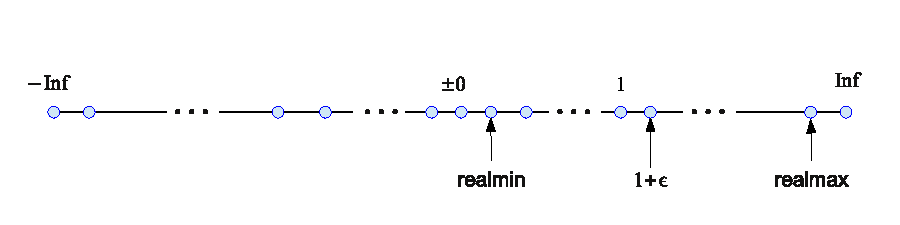
\includegraphics{01.numbers/floating-point-line.pdf}
\caption{Discreteness of floating point numbers. $\epsilon$ is the machine epsilon discussed in Sec. \ref{sec:epsilon}.}
\label{fig:machine_epsilon}
\end{figure}

\begin{example}[Special floating point numbers, Inf and NaN]\label{ex:InfNaN}
	
Anyhing bigger than \texttt{realmax} is \texttt{Inf} ("infinity") in the computer world.  Undefined number such as 0/0 is \texttt{NaN} ("Not a Number").
\small
\begin{mybox}
	\begin{verbatim}
>> realmax * 10
ans =
      Inf    
>> 0/0
ans =
      NaN
\end{verbatim}
\end{mybox}
\normalsize
\end{example}

\noindent
\exercise
Evaluate $1/0$ and $1/$\texttt{Inf}.  Are the outputs consistent with common mathematics?
\vspace{18px}

\noindent
\section{Overflow/Underflow}\label{sec:overflow}
If we try to use a value bigger than the computer can understand, what will happen? 
It results in \emph{Overflow error}.  For example, if you try to store $1.0 \times 10^{60}$ into a single precision floating point variable, the value is replaced by Inf.  Similarly, if the value is too small, it is replaced with 0.  For example, $1.0 \times  10^{-60}$ is too small for a single precision floating point. The zero may cause a problem later such as divided by zero.

In most cases, we can avoid the range errors at least for physics problems.
Many quantities have dimension and their values depend on the choice of units. Fortunately, dimensionless constants in physics are usually order of 1 or close to it. Therefore, we can avoid the range error using appropriate units.
However, there are problems which contain intrinsically large numbers without units.  For example, in statistical mechanics we often evaluate $N!$ where $N$=number particles at the order of Avogadro constant $N_A=6.02214129 \times 10^{23}$.  There is no way to compute $N!$ directly.  Even then there are tricks to calculate such large values (with help of mathematics).

We can avoid the range error in the following ways:

\begin{center}
\begin{minipage}{5in}
\begin{itemize}
\item[1.] Change the order of calculation so that large values do not appear during the calculation.
\item[2.] Use different units so that numbers are not very large or small.
For example, if \textit{atomic unit} is used, $\hbar=e=m=1$, and $\epsilon_0 = \frac{1}{4\pi}$.  The Bohr radius is simply $a_0=1$!.  In the atomic world, it is better to measure distance using the radius of hydrogen atom as a unit.  See Example \ref{ex:bohr_radius} for the calculation of $a_0$ in SI units.
\item[3.] If $x$ is too large, evaluate $y=\ln(x)$.   Then, $x=e^y$ or if base 10 is used, $x=10^y$. See Example \ref{ex:factorial}.
\end{itemize}
\end{minipage}
\end{center}

\begin{example}[Evaluation of Bohr radius]
    \label{ex:bohr_radius}
\medskip
Evaluate the Bohr radius (the radius of a hydrogen atom)\cite{Griffiths} in SI unit.    The Bohr radius is given by
$a_0 = \displaystyle\frac{4 \pi \epsilon_0 \hbar^2}{m e^2}$ where
\begin{eqnarray*}
\epsilon_0\, (\text{vacuum permittivity}) &=& 8.854187817 \times 10^{-12} F/m\\
\hbar\, (\text{Planck constant}) &=& 6.62606957 \times 10^{-34}/2\pi, m^2\, kg / s \\
m\, (\text{electron mass}) &=& 9.10938291 \times 10^{-31}\, kg\\
e\, (\text{elementary charge}) &=& 1.602176565 \times 10^{-19} C
\end{eqnarray*}

If you evaluate the numerator and denominator independently, each values may cause overflow error. By grouping the numbers in an appropriate way, you can avoid the overflow error.

\small
\begin{mybox}
\begin{verbatim}
>> epsilon=single(8.854187817e-12);
>> hbar=single(6.62606957e-34/(2*pi));
>> mass=single(9.10938291e-31);
>> e=single(1.602176565e-19);
>> a=4*pi*epsilon*hbar^2/(mass*e^2)
a =
     NaN

>> a=4*pi*(epsilon/mass)*(hbar/e)^2
a =
    5.2918e-11
\end{verbatim}
\end{mybox}
\normalsize
\end{example}

\noindent
\exercise
Evaluate the Bohr radius using double precision.  Confirm that even the dumb method causing the range error in the example is OK with double precision.
\vspace{18px}

\begin{example}[Factorial of large number]\label{ex:factorial}
Factorial of a large integer is astronomically large.  It is obviously an integer but too long to write it down.  For example, 1000! is as long as
\tiny
\begin{mybox}
\begin{verbatim}
4023872600770937735437024339230039857193748642107146325437999104299385123986290205920442084869694048004799886101971960586316668729948085589013238
2966994459099742450408707375991882362772718873251977950595099527612087497546249704360141827809464649629105639388743788648733711918104582578364784
9977012476632889835955735432513185323958463075557409114262417474349347553428646576611667797396668820291207379143853719588249808126867838374559731
7461360853795345242215865932019280908782973084313928444032812315586110369768013573042161687476096758713483120254785893207671691324484262361314125
0878020800026168315102734182797770478463586817016436502415369139828126481021309276124489635992870511496497541990934222156683257208082133318611681
1553615836546984046708975602900950537616475847728421889679646244945160765353408198901385442487984959953319101723355556602139450399736280750137837
6153071277619268490343526252000158885351473316117021039681759215109077880193931781141945452572238655414610628921879602238389714760885062768629671
4667469756291123408243920816015378088989396451826324367161676217916890977991190375403127462228998800519544441428201218736174599264295658174662830
2955570299024324153181617210465832036786906117260158783520751516284225540265170483304226143974286933061690897968482590125458327168226458066526769
9586526822728070757813918581788896522081643483448259932660433676601769996128318607883861502794659551311565520360939881806121385586003014356945272
2420634463179746059468257310379008402443243846565724501440282188525247093519062092902313649327349756551395872055965422874977401141334696271542284
5862377387538230483865688976461927383814900140767310446640259899490222221765904339901886018566526485061799702356193897017860040811889729918311021
1712298459016419210688843871218556461249607987229085192968193723886426148396573822911231250241866493531439701374285319266498753372189406942814341
1852015801412334482801505139969429015348307764456909907315243327828826986460278986432113908350621709500259738986355427719674282224875758676575234
4220207573630569498825087968928162753848863396909959826280956121450994871701244516461260379029309120889086942028510640182154399457156805941872748
9980942547421735824010636774045957417851608292301353580818400969963725242305608559037006242712434169090041536901059339838357779394109700277534720
0000000000000000000000000000000000000000000000000000000000000000000000000000000000000000000000000000000000000000000000000000000000000000000000000
0000000000000000000000000000000000000000000000000000000000000000000000000000000000000000000000000000000
\end{verbatim}
\end{mybox}
\normalsize

which is practically useless.  In fact, MATLAB retuns \texttt{Inf} for 1000!.
Therefore, we want to write it approximately in scientific notation  $a \times 10^{b}$.

In order to find the mantissa $a$ and exponent $b$, first we evaluate $\log N!$ as follows.
\begin{eqnarray}
y&=&\log(N!) = \log(1 \cdot 2 \cdot 3 \cdots N-1 \cdot N) \nonumber \\
&=& \log(1)+\log(2)+\log(3)+\cdots + \log(N-1)+\log(N)
\end{eqnarray}
Once you found $y$, $n! = e^y$.  However, it is still not in scientific notation.  First we change the base from $e$ to $10$ as $e^y  = 10^z $,  where $z = y \log_{10}(e)$.  Then, $n! = 10^z$.
Next we split $z$ to the floor k=$\lfloor z \rfloor$ and the residual $\delta=z - \lfloor z \rfloor$.
Now, we have $n! = 10^{k+\delta} = 10^\delta \times 10^k$ and thus the mantissa is $10^\delta$ and power is $k$.  Using this method, $1000! \approx 4.0239 \times 10^{2567}$. The mantissa and the power are obtained in the following way.

\bigskip
\small
\begin{mybox}
	\begin{verbatim}
>> factorial(1000)
ans =
   Inf

>> y=sum(log(1:1000))
y =
   5.9121e+03

>> z=log10(exp(1))*y
z =
   2.5676e+03
   
>> power=floor(z)
power =
    2567
    
>> mantissa=10^(z-power)
mantissa =
    4.0239
   \end{verbatim}
\end{mybox}
\normalsize
\end{example}

\noindent
\exercise
Express $10000!$ in scientific notation.

\bigskip
\noindent
\section{Machine Epsilon}\label{sec:epsilon}

Although a double precision number covers from a small number $2.2250738585072014\times 10^{-308}$ to a large number $1.7976931348623157 \times 10^{+308}$, it can distinguish only 18446744073709551616 values.  There is a gap between two closest floating point numbers.  A floating point number next to 1 is $1+\epsilon$ where $\epsilon$ is called \emph{machine epsilon}, whose value depends on the systems.  If you add a half of $\epsilon$ to 1, there is no floating point expression to the answer.  So what will happen if you try to calculate $1+\displaystyle\frac{\epsilon}{2}$. The computer thinks $1+\displaystyle\frac{\epsilon}{2} = 1$.  In the following example, you can find the machine epsilon of your computer.

\bigskip
\begin{example}[Machine epsilon built in computer language]

Most of computer languages have a function which returns the value of machine epsilon.  
Confirm that $1+\frac{\epsilon}{2} = 1$ using MATLAB command \texttt{eps()}.

\small
\begin{mybox}
	\begin{verbatim}
>> fprintf('%25.16e\n%25.16e\n%25.16e\n', eps(), 1+eps(), 1+eps()/2);
2.2204460492503131e-16
1.0000000000000002e+00
1.0000000000000000e+00
   \end{verbatim}
\end{mybox}
\normalsize
\end{example}

\bigskip
\begin{example}[Machine epsilon appears even in a simple arithmetic calculation]
	
It is easy to see that  $\displaystyle\frac{5}{3}-\frac{2}{3}-1$ and $\displaystyle\frac{7}{3}-\frac{4}{3}-1$ are both exactly zero.  However, computers don't think so.  The former vanishes as expected but the latter equals to the machine epsilon.
\small
\begin{mybox}
	\begin{verbatim}]
>> 5/3-2/3-1
ans = 0
>> 7/3-4/3-1
ans = 2.2204e-16
   \end{verbatim}
\end{mybox}
\normalsize
\end{example}

	
\bigskip
\begin{example}[Finding machine epsilon]
To find  machine epsilon, we check if $1+2^{-n}$ is bigger than $1$ for positive integer $n$.  As $n$ increases, $2^{-n}$ gets smaller and smaller.  At a certain value of $n$, it becomes too small and computer thinks $1+2^{-n} = 1$.  Then, the machine epsilon is $\epsilon = 2^{-(n-1)}$.  Program \ref{matlab:machine_epsilon}\footnote{Example codes are listed at the end of each chapter.} finds the machine epsilon using this method.  The output is 
\small
\begin{mybox}
	\begin{verbatim}
32 bit floating point
Stopped after  24 iterations 
machine epsilon by computation =    1.1920929e-07 
machine epsilon by MATLAB      =    1.1920929e-07 
1 + epsilon   =   1.00000012e+00 
1 + epsilon/2 =   1.00000000e+00 
   \end{verbatim}
\end{mybox}
\normalsize

\noindent
The value agrees with the machine epsilon obtained by MATLAB command \texttt{eps()}.
\end{example}

\noindent
\exercise
Modify Program \ref{matlab:machine_epsilon} and find the machine epsilon for double precision floating point.


\noindent
\section{Round-off Errors}\label{sec:roundoff}

When you apply some operation to two numbers such as addition, the resulting number may not exist in floating point expression.  The machine picks a nearest number.
Therefore, every operation induces some error called round-off error.  Such an error is small but accumulates over many operations and significant figures decreases after many operations. Such an error causes a fatal error when you subtract a number from a very similar number.  Suppose that two single floating point numbers have exactly the same first 5 digits.  The last two digits are not reliable due to the round-off error.  Now you subtract one from the other, only the last two digits remain in the outcome. Therefore, the outcome is not reliable at all.  You must avoid the such subtraction.

The round-off error is an serious issue for digital computers.  On February 25, 1991, during the Gulf War, an American Patriot Missile battery in Dharan, Saudi Arabia, failed to track and intercept an incoming Iraqi Scud missile. The Scud struck an American Army barracks, killing 28 soldiers and injuring around 100 other people. Patriot missile.  Round-off error is suspected to have caused this tragedy.\cite{Skeel1992} 

\bigskip
\begin{example}[Accumulation of Round-off Error]
\label{ex:manyadds}
For $x=1.2$, add $x$ 100000 times and compare the result with $100000 \times x$.  Mathematically speaking the two calculation should give the same answer.  See what your computer says.

\small
\begin{mybox}
	\begin{verbatim}
>> x=single(1.2);
>> xsum=single(0);
>>for i=1:100000
xsum=xsum+x;
end
>>xmul=single(100000)*x;
>> fprintf('Iteration=%14.7e,  Multiplication=%14.7e\n',xsum,xmul);
Iteration= 1.2011162e+05,  Multiplication= 1.2000001e+05
   \end{verbatim}
\end{mybox}
\normalsize
\end{example}


\bigskip
\noindent
\exercise
\begin{itemize}
\item[(a)]  Repeat Example \ref{ex:manyadds} with $x=2$.  The error disappears. Why?
\item[(b)]  Repeat Example \ref{ex:manyadds} using double precision.  Do you still see the round-off error?
\end{itemize}

\noindent
\section{Loss of Significance}\label{sec:significance}

Since the floating point expression of real numbers can keep only finite digits, we need to pay attention to the significant figures like we do for hand calculation with approximate numbers.  The error can be very severe particularly when two similar numbers are subtracted from one another (known as \emph{catastrophic cancellation}).  Foe examp,e let us calculate $0.123456789 \times 10^{-5} - 0.123456700 \times 10^{-5}$ using 32-bit floating point.  The exact value is $0.89 \times 10^{-12}$.   Here is the MATLAB output:

\small
\begin{mybox}
	\begin{verbatim}
>> x=single(0.123456789e-5)-single(0.123456700e-5);
>> fprintf('%16.7e',x)
9.0949470e-13
   \end{verbatim}
\end{mybox}
\normalsize
The significant figure is only one. The other digits '949470' has no significance but MATLAB prints them out as if they are a part of the answer.  If you use this number for other calculation, significant figures may be reduces to none.   The number you get may have no significance.  We need to try to avoid subtraction of similar numbers to keep the significant figures.  Note that addition has no such problem.

\begin{example}[Catastrophic cancellation]
\label{ex:twosimilarvalues}
Evaluate $\displaystyle\frac{(x+1)^2-1}{x}$ for $x$ from $10^{-1}$ to $10^{-17}$.
Compare the numerical results with the exact solution, $x+2$, which is always bigger than 2 for positive $x$.  When $x$ is smaller than machine epsilon, computer thinks that $x+1=1$ and thus the result is zero!
\small
\begin{mybox}
Script:

	\begin{verbatim}
for i=1:17
y(i)=((x(i)+1)^2-1)/x(i);
z(i)=x(i)+2;
fprintf('x=%8.1e, direct=%10.7f,  exact= %10.7f\n', x(i),y(i),z(i));
end
   \end{verbatim}

\medskip
Output:
	\begin{verbatim}
x= 1.0e-01, direct= 2.1000000,  exact=  2.1000000
x= 1.0e-02, direct= 2.0100000,  exact=  2.0100000
x= 1.0e-03, direct= 2.0010000,  exact=  2.0010000
x= 1.0e-04, direct= 2.0001000,  exact=  2.0001000
x= 1.0e-05, direct= 2.0000100,  exact=  2.0000100
x= 1.0e-06, direct= 2.0000010,  exact=  2.0000010
x= 1.0e-07, direct= 2.0000001,  exact=  2.0000001
x= 1.0e-08, direct= 2.0000000,  exact=  2.0000000
x= 1.0e-09, direct= 2.0000002,  exact=  2.0000000
x= 1.0e-10, direct= 2.0000001,  exact=  2.0000000
x= 1.0e-11, direct= 2.0000002,  exact=  2.0000000
x= 1.0e-12, direct= 2.0001778,  exact=  2.0000000
x= 1.0e-13, direct= 1.9984015,  exact=  2.0000000
x= 1.0e-14, direct= 1.9984015,  exact=  2.0000000
x= 1.0e-15, direct= 2.2204460,  exact=  2.0000000
x= 1.0e-16, direct= 0.0000000,  exact=  2.0000000
x= 1.0e-17, direct= 0.0000000,  exact=  2.0000000
   \end{verbatim}
\end{mybox}
\normalsize
\end{example} 

\noindent
\exercise
Repeat Exercise \ref{ex:twosimilarvalues} using double precision.  Reduce the value $x$ until the result deviate significantly from the exact value.

\bigskip
\begin{example}[Roots of Quadratic Equation]
	The solutions to quadratic equation $a x^2 + b x + c = 0$ are well-known:
	\begin{subequations}\label{eq:roots-original}
		\begin{equation}
		x_1 = \frac{-b - \sqrt{b^2 - 4 a c}}{2a} \label{eq:root-}
		\end{equation}
		\begin{equation}
		x_2 = \frac{-b + \sqrt{b^2 - 4 a c}}{2a}\label{eq:root+}
		\end{equation}
	\end{subequations}
	For simplicity, we assume $b>0$.
	Solution $x_1$ does not cause a serious round-off error. However, when $b^2 \gg a c$, the other solution  $x2$  involves subtraction of two similar numbers and thus it is vulnerable to catastrophic cancellation. The error is especially severe when $a \ll b$ because the denominator is very small and the situation is close to 0/0. Fortunately, there is a simple way to avoid this loss of significance. Using the equality
	\begin{equation}
	x_2 = \frac{-b + \sqrt{b^2 - 4 a c}}{2a} = \frac{-2c}{b+\sqrt{b^2 - 4 a c}} = \frac{c}{a x_1}
	\label{eq:quad_trick1}
	\end{equation}
	the subtraction causing catastrophic cancellation disappears.  Similarly for $b<0$, Eq. \eqref{eq:root-} which may cause catastrophic cancellation can be evaluated by 
	\begin{equation}
	x_1 = \frac{-b - \sqrt{b^2 - 4 a c}}{2a} = \frac{-2c}{-b+\sqrt{b^2 - 4 a c}} = \frac{c}{a x_2}.
	\label{eq:quad_trick2}
	\end{equation}
	There are many pitfalls with the floating point numbers.  See more examples in Ref. \cite{Goldberg1991}.
	
\bigskip
\begin{myalgobox}
	\Algorithm{Roots of Quadratic Equation}\label{algo:roots-quad}

\bigskip
Roots of $a x^2 + b x + c = 0$ ($a \ne 0$ and $b \ne 0$).
\begin{eqnarray}
x_1 &=& \frac{-b - \text{sgn}(b)\sqrt{b^2 - 4 a c}}{2a} \\
x_2 &=& \frac{c}{a x_1}
\end{eqnarray}
where
\[
\sign(b) = \begin{cases} +1 & b>0 \\ -1 & b<0 \end{cases}
\]
\end{myalgobox}

\end{example}

\bigskip

\noindent
\section*{Problems}
\addcontentsline{toc}{section}{\protect\numberline{}Problems}

\begin{enumerate}[labelwidth=0.5cm,labelindent=0.0cm,leftmargin=*,label=\bfseries \thechapter.\arabic*,align=left]
\item
Evaluate the roots of $a x^2 + x + \displaystyle\frac{1}{4} = 0$ using the original formula Eqs. \eqref{eq:roots-original} and Algorithm \ref{algo:roots-quad}. Reduce the value of $a$ as 0.1, 0.01, 0.001, $\cdots$ until it hits the machine epsilon. Note that the exact answer for $a=0$ is $x=-\displaystyle\frac{1}{4}$.  Observe that the original formula fails but the improved one works.
\item In statistical mechanics, factorial $n!$ of huge integer $n$ such as the Avogadro number often appears. It is difficult to manage such a huge number even analytically.  A common method to deal with such problem is to use the Stirling formula\cite{Zwillinger2012}:
\begin{equation}
\ln(n!) \approx n \ln(n) - n + \frac{1}{2} \ln(2 \pi n)
\label{eq:stirling1}
\end{equation}
Then, the factorial can be approximated by
\begin{equation}
n! \approx \sqrt{2 \pi n} \left ( \frac{n}{\text{e}} \right )^n\, .
\label{eq:stirling2}
\end{equation}
To verify the accuracy of this formula, compute the ratio $R=\displaystyle\frac{n!}{\sqrt{2 \pi n} \left ( \frac{n}{\text{e}} \right )^n}$  for $n=10, 100$, and $1000$.  Verify that formula (\ref{eq:stirling2}) approaches the exact value as $n$ increases. Note that direct calculation of $R$ is hard but $\ln R$ can be easily evaluated.
\end{enumerate}


\vspace{1 in}
\noindent
\section*{Examples in Python}
\addcontentsline{toc}{section}{\protect\numberline{}Examples in Python}


The core of \texttt{Python} does not have much of mathematical capabilities. It relies on modules.  Here we use a popular mathematical module, \texttt{NumPy}.
You need to load the module before using mathematical objects. In this lecture note, it is assumed that \texttt{NumPy} is loaded in the following way.
\small
\begin{mybox}
	\begin{verbatim}
>>> import numpy as np
   \end{verbatim}
\end{mybox}
\normalsize
Hereafter it is assumed that numpy is imported as np.

\bigskip
\setcounter{exampnum}{0}
\noindent
\textbf{\ref{sec:integer} Integer}

\bigskip

\texttt{Python} has 4 classes of unsigned integer, \texttt{uint8},
\texttt{uint16},  \texttt{uint32}, and  \texttt{uint64}.  Similarly, there are 4 classes of signed integer, \texttt{int8},
\texttt{int16},  \texttt{int32}, and  \texttt{int64}.
In \texttt{NumPy} functions \texttt{iinfo().max} and \texttt{iinfo().min} return the smallest and largest integer values of the specified class. 

\begin{example}[Maximum and minimum of integers]
\small
\begin{mybox}
	\begin{verbatim}
In: np.iinfo(np.int16).max
Out: 32767
In: np.iinfo(np.int16).min
Out: -32768
   \end{verbatim}
\end{mybox}
\normalsize
\end{example}

\noindent
\begin{example}[Identify the type]
\small
\begin{mybox}
	\begin{verbatim}
In: y=2
In: type(y)
Out: int

In: y=2.
In: type(y)
Out: float
   \end{verbatim}
\end{mybox}
\normalsize
\end{example}

\bigskip
\textbf{\ref{sec:characters} Characters}
\bigskip
\begin{example}[Character-number conversion]
\small
\begin{mybox}
	\begin{verbatim}
In: str(12)
Out: '12'
In: int('12')
Out: 12
   \end{verbatim}
\end{mybox}
\normalsize
\end{example}

\bigskip
\textbf{\ref{sec:float} Floating Point Numbers}
\bigskip

\texttt{Python} has 4 classes of floating point number.
\texttt{float16},  \texttt{float32}, \texttt{float64} and \texttt{float128}.  The true \texttt{float128} is not available on common computers.  If it is used, \texttt{float128} is actually mapped to 80-bit float on common 64-bit hardware. (Math co-processor on Intel 64-bit CPU uses 80-Bit floating point number.)  In \texttt{NumPy} functions \texttt{finfo().max} and \texttt{finfo().min} return the smallest and largest integer values of the specified class.

\begin{example}[Range of floating point numbers]
\small
\begin{mybox}
	\begin{verbatim}
# Print the smallest and largest double precision value.
In: print("{0:25.16e},{1:25.16e}".format(np.finfo(float).min),np.finfo(float).max)  
Out: -1.7976931348623157e+308, 1.7976931348623157e+308
   \end{verbatim}
\end{mybox}
\normalsize
\end{example}

\newpage

\begin{example}[Special floating point numbers, Inf and NaN]

If numpy is not used, Python returns an error message instead of 
\texttt{inf}.
\small
\begin{mybox}
	\begin{verbatim}
In: x=np.finfo(float).max
In: x*10
__main__:1: RuntimeWarning: overflow encountered in double_scalars
Out: inf

In: np.float64(1.0)/0.0
__main__:1: RuntimeWarning: divide by zero encountered in double_scalars
Out: inf

In: np.float64(0.0)/0.0
__main__:1: RuntimeWarning: invalid value encountered in double_scalars
Out: nan

In: 1.0/0.0
Traceback (most recent call last):
File "<ipython-input-34-0dda708f6d03>", line 1, in <module>
1.0/0.0
ZeroDivisionError: float division by zero
   \end{verbatim}
\normalsize
\end{mybox}
\end{example}

\textbf{\ref{sec:overflow} Overflow/Underflow}

\begin{example}[Evaluation of Bohr radius]

	Python behaves quite differently from other languages.  The product of two numbers in float32 is usually again a number in float32.  In most languages this is a strict rule.  Python observes the same rule unless the outcome causes underflow error.  When the underflow happened, Python automatically switches to float64.  This may be a convenient feature but it is also annoying as well since the programmer cannot control it.  In the following, we force output to the float32 type. 

\small
\begin{mybox}
Script:
\begin{verbatim}
import numpy as np

# Set the parameter values
pi=np.float32(np.pi)
epsilon=np.float32(8.854187817e-12)
hbar=np.float32(6.62606957e-34/(2*pi))
mass=np.float32(9.10938291e-31)
e=np.float32(1.602176565e-19)

# Evaluate the denominator and numerator separately. 
y=np.float32(mass*e**2) 
x=np.float32(4.*pi*epsilon*hbar**2) 
print("a=",np.float32(x/y))
\end{verbatim}

\medskip
Output:
\begin{verbatim}
a= nan
\end{verbatim}

\bigskip
Script:
\begin{verbatim}
# Evaluate them in a different order
>>> x=4.*pi*(epsilon/mass)
>>> y=np.float32((hbar/e)**2)
>>> print("a=",np.float32(x*y)) 
\end{verbatim}

\medskip
Output:
\begin{verbatim}
a= 5.29177e-11 
\end{verbatim}
\end{mybox}
\normalsize
\end{example}

\newpage
\noindent
\begin{example}[Factorial of large number]

\small
\begin{mybox}
	\begin{verbatim}
In: np.float(np.math.factorial(1000))
Traceback (most recent call last):
  File "<stdin>", line 1, in <module>
OverflowError: int too large to convert to float

In: y=np.log(np.arange(1,1001)).sum();y
Out: 5912.128178488163

In: z=np.log10(np.exp(1))*y; z
Out: 2567.6046442221327
   
In: power=np.int(np.floor(z)); power
Out: 2567
    
In: mantissa=10**(z-power); mantissa
Out: 4.0238726007697423
   \end{verbatim}
\end{mybox}
\normalsize

\medskip\noindent
Hence, $1000! \approx 4.0238726008 \times 10^{2567}$.  
\end{example}

\bigskip
\textbf{\ref{sec:epsilon} Machine Epsilon}

\begin{example}[Machine epsilon built in computer language]

\small
\begin{mybox}
	\begin{verbatim}
>>> print("{0:25.16e}\n{1:25.16e}\n{2:25.16e}".format(np.finfo(float).eps,
... 1+np.finfo(float).eps,1+np.finfo(float).eps/2))
   2.2204460492503131e-16
   1.0000000000000002e+00
   1.0000000000000000e+00
   \end{verbatim}
\end{mybox}
\normalsize
\end{example}

\noindent
\begin{example}[Machine epsilon appears even in a simple arithmetic calculation]
	
\small
\begin{mybox}
	\begin{verbatim}
In: 5./3.-2./3.-1.
Out: 0.0
In: 7./3.-4./3.-1.
Out: 2.220446049250313e-16
   \end{verbatim}
\end{mybox}
\normalsize
\end{example}

\noindent
\begin{example}[Finding machine epsilon]

Output from example code: \texttt{ch01pr01.py}.

\small
\begin{mybox}
	\begin{verbatim}

Machine epsilon for 64 bit floating point
Stopped after  53 itersations
machine epsilon by computation =    2.2204460e-16
machine epsilon by Numpy       =    2.2204460e-16
1+epsilon   = 1.00000000000000022204e+00
1+epsilon/2 = 1.00000000000000000000e+00
   \end{verbatim}
\end{mybox}
\normalsize
\end{example}


\textbf{\ref{sec:roundoff} Round-off Error}

\begin{example}[Accumulation of Round-off Error]

\small
\begin{mybox}
Script:
\begin{verbatim}
x=np.float32(1.2)
xsum=np.float32(0.0)
for i in range(1,100001):
	xsum=xsum+x

xmul=np.float32(100000.)*x
print("Iteration={0:14.7e}, Multiplication={1:14.7e}".format(xsum,xmul))
\end{verbatim}

\medskip
Output:
\begin{verbatim}
Iteration= 1.2011162e+05, Multiplication= 1.2000001e+05
\end{verbatim}
\end{mybox}
\normalsize
\end{example}

\bigskip
\textbf{\ref{sec:significance} Loss of Significance}

\small
\begin{mybox}
	\begin{verbatim}
In:  np.float32(0.123456789e-5)-np.float32(0.123456700e-5)
Out: 9.094947e-13
   \end{verbatim}
\end{mybox}
\normalsize

\newpage
\noindent
\begin{example}[Catastrophic cancellation]
	
\small
\begin{mybox}
Script:
\begin{verbatim}
x=np.float32(10**(-i))
y=((x+1)**2-1)/x
z=x+2
print("x={0:8.1e}, direct={1:10.7f}, exact={2:10.7f}".format(x,y,z))
\end{verbatim}

\medskip
Output:
\begin{verbatim}
x= 1.0e-01, direct= 2.1000000, exact= 2.1000000
x= 1.0e-02, direct= 2.0100000, exact= 2.0100000
x= 1.0e-03, direct= 2.0010000, exact= 2.0010000
x= 1.0e-04, direct= 2.0001000, exact= 2.0001000
x= 1.0e-05, direct= 2.0000100, exact= 2.0000100
x= 1.0e-06, direct= 2.0000010, exact= 2.0000010
x= 1.0e-07, direct= 2.0000001, exact= 2.0000001
x= 1.0e-08, direct= 2.0000000, exact= 2.0000000
x= 1.0e-09, direct= 2.0000002, exact= 2.0000000
x= 1.0e-10, direct= 2.0000001, exact= 2.0000000
x= 1.0e-11, direct= 2.0000002, exact= 2.0000000
x= 1.0e-12, direct= 2.0001778, exact= 2.0000000
x= 1.0e-13, direct= 1.9984015, exact= 2.0000000
x= 1.0e-14, direct= 1.9984015, exact= 2.0000000
x= 1.0e-15, direct= 2.2204460, exact= 2.0000000
x= 1.0e-16, direct= 0.0000000, exact= 2.0000000
x= 1.0e-17, direct= 0.0000000, exact= 2.0000000
\end{verbatim}
\end{mybox}
\normalsize
\end{example}

\bigskip
\noindent
\section*{MATLAB Source Codes}
\addcontentsline{toc}{section}{\protect\numberline{}MATLAB Source Codes}
\setcounter{program}{0}
\noindent
\program\label{matlab:machine_epsilon}

\bigskip
\footnotesize
\begin{verbatim}
%*********************************************************************
%*     Example  1.7                                                  *
%*     filename: ch01pr01.m                                          *
%*     program listing number: 1.1                                   *
%*                                                                   *
%*     This program finds a machine epsilon by evaluating            *
%*                                                                   *
%*           1 + 2^(-n) > 1                                          *
%*                                                                   *
%*     At a certain positive n, this inequality becomes false.       *
%*     Then, the machine epsilon is 2^(n-1).                         *
%*                                                                   *
%*     Programed by Ryoichi Kawai for Computational Physics Course   *
%*     Revised on 10/13/2013                                         *
%*********************************************************************

clear all;  help ch01pr01;

%* Find the single precision machine epsilon
epsilon = single(1);  % create a single precision variable
n = int8(0);            % reset a counter

%* Reduce the value of epsilon until epsilon becomes too small
while 1+epsilon > 1
   epsilon = epsilon/2;
   n = n+1;
end

%* The smallest single floating value which can be added to one.
epsilon = epsilon+epsilon;

%* Show the results
fprintf('\n32 bit floating point\n');
fprintf('Stopped after %3d iterations \n',n);
fprintf('machine epsilon by computation = %16.7e \n',epsilon);
fprintf('machine epsilon by MATLAB      = %16.7e \n',eps(single(1.0)));
fprintf('1 + epsilon   = %16.8e \n',1+epsilon);
fprintf('1 + epsilon/2 = %16.8e \n',1+epsilon/2);
\end{verbatim}
\normalsize

\bigskip
\section*{Python Source Codes}
\addcontentsline{toc}{section}{\protect\numberline{}Python Source Codes}
\setcounter{program}{0}
 
\bigskip
\noindent
\program\label{python:machine_epsilon}

\footnotesize
\begin{verbatim}
"""
%*********************************************************************
%*     Example  1.7                                                  *
%*     filename: ch01pr01.py                                         *
%*     program listing number: 1.1                                   *
%*                                                                   *
%*     This program finds a machine epsilon by evaluating            *
%*                                                                   *
%*           1 + 2^(-n) > 1                                          *
%*                                                                   *
%*     At a certain positive n, this inenqualty becomes false.       *
%*     Then, the machine epsilon is 2^(n-1).                         *
%*                                                                   *
%*     Programed by Ryoichi Kawai for Computational Physics Course   *
%*     Revised on 12/27/2016                                         *
%*********************************************************************
"""

# Find the machine epsilon for 64 bit float
epsilon = 1.0  # create a float64 variable
n = 0          # reset a counter

# Reduce the value of epsilon until it becomes too small
while 1.0+epsilon > 1.0:
   epsilon = epsilon/2.0
   n = n+1

# The smallest single floating value which can be added to one.
epsilon = epsilon+epsilon

# Show the results
print("Machine epsilon for 64 bit floating point")
print("Stopped after {0:3d} itersations".format(n))
print("machine epsilon by computation = {0:16.7e}".format(epsilon))
print("machine epsilon by Numpy       = {0:16.7e}".format(np.finfo(np.float).eps))
print("1+epsilon   = {0:24.20e}".format(1+epsilon))
print("1+epsilon/2 = {0:24.20e}".format(1+epsilon/2.0))
\end{verbatim}

\normalsize
\vfill



%\chapbibliography
\bibliographystyle{unsrt}
\bibliography{compphys}


\chapter{Numerical Derivatives}\label{ch:derivatives}

When we study physics, we often investigate the change of certain quantities.  That is why basic calculus plays a major role in physics.  Evaluating the derivative of a function $f(x)$ is an ubiquitous operation in physics.  However, an analytical expression of the derivative is not always available.  Then, a numerical method must be deployed to evaluate it.  That is not only the reason we need numerical derivative.  In some cases an analytical expression of the function itself is not available.  For example, when a function is experimentally obtained by measurement, it is given as a set of numerical data, $(x_i, f_i),\, i=1, \cdots, N$.  Then, analysis of such data is always numerical.  There are many algorithms for numerical derivative.  In this chapter, we study some of well-known algorithms useful for studying physics.

Numerical methods are in general not exact and involve systematic errors.  Understanding the source of errors and their magnitude is very important.  It is possible to estimate the magnitude of expected errors based on mathematical analysis and the study of numerical error is an important part of numerical analysis.  We will investigate the degrees of errors through theory and examples.

In this section, we assume that an analytical expression of function $f(x)$ is given and that we can numerically evaluate it at any point $x$. Furthermore, we assume that the numerical error in the evaluation of the function is negligiblly small.  In other words, the main errors occur when the derivative is evaluated. 


\section{First order derivatives}\label{sec:dv-1st-order}
\begin{figure}
\centerline{\includegraphics[width=3in]{02.derivatives/diff.pdf}}
\caption{Illustration of various numerical derivatives.  The exact derivative is the slope of the curve at $x$, which is shown as the dotted line. The forward finite difference method shown in green  underestimates the slop whereas the backward finite difference method shwon in blue overestimates it.  The mean finite different method shown in red looks very close to the exact derivative.}
\label{fig:diff}
\end{figure}
  
Let us look at the mathematical definition of derivative:
\begin{equation}\label{eq:diff_exact}
\dv{x} f(x) = \lim_{h \searrow 0} \frac{f(x+h)-f(x)}{h} = \lim_{h \searrow 0} \frac{f(x)-f(x-h)}{h}
\end{equation}
which involves limit operation which floating point calculation cannot not perform due to the quantization (See Chap. \ref{ch:numbers}).
If $h=0$ is used, we have \texttt{0/0=NaN}.
If $h$=\texttt{realmin} is used, $f(x+h)-f(x)$ is very inaccurate due to round-off error as discussed in Chapter \ref{ch:numbers}.
If  $1 \gg h >$ \texttt{realmin} is used, the both numerator and denominator are finite but the ratio is not exactly the limit.  

It is clear that direct numerical evaluation of Eq \eqref{eq:diff_exact} is not possible. 
However,  it is expected to be close to the limit if an \textit{appropriately small} value of $h$ is used.  
Based on this naive argument, we hope that the following \textit{forward finite difference} method is close to the actual derivative with a certain small value of $h$.
\begin{equation}\label{eq:diff_fwd}
\dv{x} f(x) \approx \Delta_\text{F} f(x)  \equiv \fbox{$\displaystyle \frac{f(x+h)-f(x)}{h}$}\, .
\end{equation}
where $\Delta_\text{F}$ is the forward finite difference operator. 
Similarly, we define the \textit{backward finite difference} method
\begin{equation}\label{eq:diff_bwd}
\dv{x} f(x) \approx \Delta_\text{B} f(x) \equiv \fbox{$\displaystyle \frac{f(x)-f(x-h)}{h}$}\, .
\end{equation}
where $\Delta_\text{B}$ is the backward finite difference operator. 
Unlike the exact limit (\ref{eq:diff_exact}) the forward and backward finite difference methods do not agree each other due to the finite $h$.
As illustrated in Fig. \ref{fig:diff}, one of them overestimates and the other underestimates.  

Now, we investigate how accurate the forward and backward finite difference methods are. We estimate the order of error using Taylor expansion\cite{Boas2006},
\begin{subequations}\label{eq:h.expand}
\begin{equation}
f(x+h) = f(x) + h\, f'(x) + \frac{h^2}{2} f''(x) + \frac{h^3}{3!} f^{(3)}(x) + \order{h^4}\label{eq:h+expand}
\end{equation}
\begin{equation}
f(x-h) = f(x) - h\, f'(x) + \frac{h^2}{2} f''(x) - \frac{h^3}{3!} f^{(3)}(x) + \order{h^4}\label{eq:h-expand}
\end{equation}
\end{subequations}
where $\order{h^4}$ mean that the remaining terms with $h^4$ and higher order.

Substituting the expansions \eqref{eq:h.expand} to Eqs. \eqref{eq:diff_fwd} and \eqref{eq:diff_bwd}), we find
\begin{subequations}\label{eq:derivative_error}
	\begin{equation}
    \Delta_\text{F} f(x) =  f'(x) + \frac{h}{2} f''(x) + \order{h^2}
    \end{equation}
    \begin{equation}
    \Delta_\text{B} f(x) =  f'(x) - \frac{h}{2} f''(x) + \order{h^2}  
    \end{equation}
\end{subequations}
where $f'$ and $f''$ indicate the first and second order derivatives of $f$. The leading term in the error $ \Delta_\text{F,B} f(x) - f'(x)$ is $\pm  \frac{h}{2} f''(x)$, which is the order of $h$. This means that if $h$ is small enough, the numerical methods agree with the exact derivative. However, the error decreases only linearly with $h$.  We need to remember that if $h$ is too small, the round-off error kills the accuracy.  Hence, $h$ cannot be too small.  Error at the order $h$ is in general not acceptable and these methods are not accurate enough for practical applications.

There is a better method.  Noting that the error in the forward and backward finite difference method is exactly the same in magnitude but has opposite sign, we can get rid of the error at the order of $h$.
Taking the mean of the two approximations, we obtain
\begin{equation}\label{eq:diff_mid}
\Delta_\text{M} f(x) \equiv \frac{\Delta_\text{F} f(x)+\Delta_\text{B} f(x)}{2} = \fbox{$\displaystyle\frac{f(x+h)-f(x-h)}{2h}$}\, .
\end{equation}
where $\Delta_\text{M}$ is a \textit{mean finite difference} operator.

Substituting the expansions \eqref{eq:h.expand} to \eqref{eq:diff_mid}, we find
\begin{equation}\label{eq:derivative_error_mean}
\Delta_\text{M} f(x) = f'(x) + \frac{h^2}{3!} f^{(3)}(x) + \order{h^4}
\end{equation}
Now, the error is at the order of $h^2$ which is smaller than the previous error at $h$. 
The improvement is clearly visible in Fig. \ref{fig:diff}.  

Mathematically speaking, the small error in the mean finite difference method is related to the mean value theorem\cite{mean_value_theorem} which states that there is at least one number $c$ between $a$ and $b$ such that
\begin{equation}\label{eq:mean-value-theorem}
f'(c)=\frac{f(b)-f(a)}{b-a}
\end{equation} 
Let $b=x+h$ and $a=x-h$,  the right hand side of Eq \eqref{eq:mean-value-theorem} mathces to $\Delta_\textbf{M}f(x)$.  Therefore, the mean finite different method gives the slope of the curve at some point $c$ between $x+h$ and $x-h$.  When $h$ is small, $c$ is apprximately $x$.  Then, we obtain the mean finite difference formula \eqref{eq:diff_mid}.


The mean finite element method \eqref{eq:diff_mid} is good enough for most application.
If even a higher degree of accuracy is needed, use the symmetric four-point method\cite{Zwillinger2012}
\begin{equation}
\Delta_{S4} f(x) \equiv \fbox{$\displaystyle\frac{f(x+2h) - 8 f(x+h) + 8 f(x-h) - f(x - 2h)}{12 h}$}\, .
\end{equation}
Its error is at the order of $h^4$. 

\vspace{18px}
\noindent
\exercise
Using the Taylor expansion, verify that the error of symmetric four-point method is order of $h^4$.
\vspace{18px}

How do we find an appropriate value of $h$?
Considering the definition of derivative (\ref{eq:diff_exact}), one might expect that smaller $h$ provides more accurate result. However, when $h$ is too small, the finite different methods suffer from the round-off error.  Therefore, we must choose the value of $h$  carefully, not too big and not too small. Noting that $x+h = x (1+x/h)$, it is pointless to use $h < \epsilon_\text{m}\, x$ where $\epsilon_\text{m}$ is the machine epsilon. (See Section 1.6
%%%Cross Refernce \ref{sec:epsilon} %%%
). Example \ref{ex:derivatives} illustrates that the finite difference method fails when $h$ is too small. 


\bigskip
\begin{example}[Round-off errors in finite difference methods]\label{ex:derivatives}
Let's numerically evaluate the derivative of $f(x)=\displaystyle\frac{1}{3}x^3$ at $x=1$ and compare the results with the exact value.
The analytic form of derivative is $f'(x)=x^2$ and thus the exact value is $f'(1)=1$.  Program \ref{prog:derivative} computes the derivative using the forward, backward and mean finite difference methods for
$h=1, 0.1, 0.01, \cdots, 10^{-19}$.  The error is measured by $\delta = |f'(1)-\Delta f(1)|$.  The results are plotted in Fig.
\ref{fig:derivatives}.  The error of forward and backward methods is almost the same and decreases in the same way as $h$.  However, the improvement stop at $h \sim 10^{-8}$ and the error increases for smaller $h$ due to the round-off error. The best answer is obtained with $h=10^{-8}$. The mean difference method shows much better result.  The error decreases with $h^2$.  The best value is obtained at $h=10^{-5}$ and the result is better than the best value obtained by the forward or backward method.  It is quite clear that the mean difference method is much better than the two others.
\begin{figure}[t]
\centerline{\includegraphics[width=6.0in]{02.derivatives/derivative-plot.pdf}}
\caption{Output of Example \ref{ex:derivatives}.  The left panel shows numerical derivatives for wide ranges of $h$.  As $h$ decreases from $h=1$ to $h=0.01$, the derivative converges to 1 (at least in our eyes). As $h$ further decreases, the values of all methods remain the same until $h \approx \epsilon_\text{m}$.  Below it, the derivative abruptly goes to 0.  The numerical method fails due to round-off error. To see more details, the right panel plots the error. As $h$ decreases, the error of the forward and backward finite difference methods decreases in the same way as $h$ until $h \approx 10^{-8}$ but the error increases when $h$ is further reduced.  The mean finite difference method shows smaller error than the two other methods and the error decreases as $h^2$ up to $h \sim 10^{-5}$.  The best result is given by the mean finite difference method with $h \approx 10^{-5}$.}
\label{fig:derivatives}
\end{figure}
\end{example}
\bigskip

In practice, we don't know the actual error and therefore we cannot use a plot like the right panel of Fig. \ref{fig:derivatives} to find an appropriate value for $h$.  However, the left panel of Fig. \ref{fig:derivatives} shows that the numerical derivative approaches a certain value and the output does not change much when $h$ is smaller than a certain value until it hits the limit of round-off error.
Suppose that we calculate the derivative using $h$ and $h'=h/2$.  We expect that the output is more accurate with $h'$ than $h$. Using Eq. (\ref{eq:derivative_error_mean}), the change of the mean finite difference is given by
\begin{equation}
\left | \Delta_\text{M} f(x) - \Delta'_\text{M} f(x) \right | = \frac{|f^{(3)}|}{3!} \frac{3}{4} h^2 = \frac{3}{4} \times  \left [ \text{error in } \Delta_\text{M} f(x) \right ]
\end{equation}
which suggests that the error is estimated by
\begin{equation}
\text{Error in }\Delta_M f(x) \approx  \left | \Delta_\text{M} f(x) - \Delta'_\text{M} f(x) \right |  
\end{equation}. 
Note that the exact value of $f'(x)$ is not needed to find the error.
Now we have an algorithm to find numerical derivative with a desired accuracy using this error estimate.  

\bigskip

\begin{myalgobox}
\Algorithm{Numerical derivative with tolerance}\label{algo:derivative-auto}

\medskip
\begin{enumerate}
\item Set a value of \textit{tolerance} (allowed error).
\item Set a reference step size $h_1$ and evaluate a reference derivative $g_1 = \Delta_\text{M} f(x)$ using $h_1$.
\item Set a new step size $h_2=h_1/2$ and evaluate a new derivative $g_2 = \Delta_\text{M} f(x)$ using $h_2$.
\item Evaluate error $\delta = |g_2-g_1|$.
\item If $\delta < \text{tolerance}$, $g_2$ is the desired result.  Stop the loop.
\item If not, let $g_1=g_2$ and $h_1=h_2$ (previous $g_2$ and $h_2$ are now the reference).
\item Go back to Step 3.
\end{enumerate}
\end{myalgobox}


\bigskip\noindent
Here the absolute error is used.  We can also use a relative error $\left |\displaystyle \frac{g_2 - g_1}{g_1} \right |$ instead. Then, the tolerance specifies a desired relative error. 

\begin{example}[Automatic adjustment of the step size $h$.]
We numerically evaluate the derivative of  $f(x)=\displaystyle\frac{1}{3}x^3$ at $x=1$ again.  This time, we do not specify the step length $h$. Instead we specify a tolerance and the program will automatically find an appropriate $h$ for the given tolerance.  Program \ref{prog:derivative-auto} implements Algorithm \ref{algo:derivative-auto}.  When the tolerance is 0.001, we obtain the following output.
It appears that $h=0.03125$ is good enough for this problem.  



\begin{mybox}
\small
\begin{verbatim}
Enter tolerance =0.001
    h       derivative            error
 5.000e-01 1.0833333333e+00 2.5000000000e-01
 2.500e-01 1.0208333333e+00 6.2500000000e-02
 1.250e-01 1.0052083333e+00 1.5625000000e-02
 6.250e-02 1.0013020833e+00 3.9062500000e-03
 3.125e-02 1.0003255208e+00 9.7656250000e-04
Tolerance is OK.
\end{verbatim}
\normalsize
\end{mybox}
\end{example}

\vspace{18px}
\noindent
\exercise
Evaluate of the derivative of $\sin(x)$ at $x=\pi/4$ using the mean finite difference method.  The first three digits of the answer should be correct.

\vspace{18px}

\noindent
\section{Second order derivatives}

We can evaluated the second order derivative using the mean value method twice.
First, we pretend that the first order derivative is given. Using the mean value method with step size $h/2$, we obtain
\begin{equation}
f''(x) \approx \Delta_M f'(x) = \frac{f'(x+\frac{h}{2})-f'(x-\frac{h}{2})}{h}
\end{equation}
Then, we replace the first order derivatives with approximated ones using the mean value method again.
\begin{subequations}
\begin{equation}
f'(x+\frac{h}{2}) \rightarrow \Delta_M f(x+\frac{h}{2}) = \frac{f(x+h)-f(x)}{h}
\end{equation}
\begin{equation}
f'(x-\frac{h}{2}) \rightarrow \Delta_M f(x-\frac{h}{2}) = \frac{f(x)-f(x-h)}{h}.
\end{equation}
\end{subequations}
The result is
\begin{equation}\label{eq:diff2-s3}
f''(x) \approx \Delta^{(2)}_M f(x) \equiv \fbox{$\displaystyle\frac{f(x+h)+f(x-h)-2f(x)}{h^2}$}.
\end{equation}
where $\Delta^{(2)}_M$ is the second order mean finite difference operator.
Substituting Eqs. (\ref{eq:h+expand}) and (\ref{eq:h-expand}) into (\ref{eq:diff2-s3}), we find that the error of this approximation is order of $h^2$.  

\vspace{18px}
\noindent
\exercise
The second order derivative of $\sin(x)$ is $-\sin(x)$.  Evaluate the second order derivative of $\sin(x)$ at $x=2 n \pi / N$ where $n=0, 1, \cdots, N$.  Use $N=100$ and plot the result. Verify that it is $-\sin(x)$ at least within the accuracy of the numerical method.

\vspace{18px}

If a higher accuracy is needed, use the symmetric five-point method
\begin{equation}\label{eq:diff2-s5}
f''(x) \approx \Delta^{(2)}_{S5} f(x) \equiv \fbox{$\displaystyle\frac{-f(x+2h) + 16 f(x+h) - 30 f(x) + 16 f(x-h) - f(x-2 h)}{12 h^2}$}
\end{equation}
whose error is the order of $h^4$.\cite{diff2}

\vspace{18px}
\noindent
\exercise
Using the Taylor expansion, verify that the error of symmetric five-point method is order of $h^4$.

\vspace{18px}



\noindent
\section*{Problems}
\addcontentsline{toc}{section}{\protect\numberline{}Problems}

\begin{enumerate}[labelwidth=0.5cm,labelindent=0cm,leftmargin=*,label=\bfseries \thechapter.\arabic*,align=left]
	
\item Evaluate the first order derivative of $\sin(x)$ for interval $(0,2\pi)$ with tolerance 0.0001. What value of $h$ is needed to satisfy the tolerance?  Compare the numerical derivative with the exact one $\cos(x)$ and check if the tolerance is indeed satisfied. 
\item Evaluate the second order derivative of $f(x)=\displaystyle\frac{1}{12} x^4$ at $x=1$ using $h=1, 0.1, 0.01, \cdots, 10^{-10}$.
Plot the error as a function of $h$. Plot also the theoretical error $h^2$ for the three-point method \eqref{eq:diff2-s3}. [Optional: Try also the five-point method \eqref{eq:diff2-s5} and check how the error increases.  Unexpectedly, the larger $h$ gives better answer.  The symmetric five-point formula takes into account up to the fourth order derivative. The fifth and higher order derivative of $x^4$ vanishes and thus the five-point formula is theoretically exact for $x^4$.  Nevertheless, you encounter numerical errors due to the loss of significance.  Therefore, the larger $h$ is better for this particular function.  Try the same calculation with $f(x)=\displaystyle\frac{1}{20}x^5$. You will see the usual error profile.]
%
\end{enumerate}

\vspace{1 in}
\bigskip
\noindent
\section*{MATLAB Source Codes}
\addcontentsline{toc}{section}{\protect\numberline{}MATLAB Source Codes}
\setcounter{program}{0}

\bigskip
\noindent
\program\label{prog:derivative}

\footnotesize
\begin{verbatim}
%**************************************************************************
%*     Example  2.1                                                       *
%*     filename: ch02pr01.m                                               *
%*     program listing number: 2.1                                        *
%*                                                                        *
%*  This program evaluates the derivative of a given function func(x)     *
%*  at x=1 using the three finite difference methods.                     *
%*  Errors in forward, backward and mean value methods are plotted.       *
%*                                                                        *
%*     Programed by Ryoichi Kawai for Computational Physics Course.       *
%*     Last modification:  12/25/2013.                                    *
%**************************************************************************
clear all;

% define the function
func = @(x) x^3/3;

x=1;  % the point at which derivative is evaluated.
imax=20; % number of different displacements

% title and headers
display('Absolute Errors')
fprintf('%4s %16s %18s %20s\n','h','forward','backward','mean value')

for i=1:imax
    
    % Small displacement
    h(i)=10^(-i+1);
    
    % Evaluation of numerical derivative
    d_f(i)=(func(x+h(i))-func(x))/h(i); % Forward diffrence
    d_b(i)=(func(x)-func(x-h(i)))/h(i); % Backward diffrence
    d_m(i)=(func(x+h(i))-func(x-h(i)))/(2*h(i)); % Mean value
    
    % Errors
    err_f(i)=abs(1-d_f(i));
    err_b(i)=abs(1-d_b(i));
    err_m(i)=abs(1-d_m(i));
    
    % Display the errors
    fprintf('%6.1e %18.10e %18.10e %18.10e\n',...
            h(i),err_f(i),err_b(i),err_m(i));
end

hh = h.*h; % h^2 (the error of the mean value formula is order of h^2)

% Plot data
subplot(1,2,1)  % left panel
q=semilogx(h(1:imax),d_b(1:imax),'-o',...
    h(1:imax),d_f(1:imax),'-d',...
    h(1:imax),d_m(1:imax),'-s');
title('Numerical Derivative');
xlabel('h','fontsize',14);
ylabel('Derivative','fontsize',14);
set(q(1),'Color','blue');
set(q(2),'Color','green');
set(q(3),'Color','red');    
legend(q,{'forward','backward','mean'});
legend(q,'Location','NorthWest');

subplot(1,2,2) % right panel
p=loglog(h(1:imax),err_b(1:imax),'o',...
    h(1:imax),err_f(1:imax),'d',...
    h(1:imax),err_m(1:imax),'s',...
    h(1:imax/2),h(1:imax/2),'--',h(1:imax/2),hh(1:imax/2),'--');
title('Errors in the finite difference methods');
xlabel('h','fontsize',14);
ylabel('absolute error','fontsize',14);
set(p(1),'Color','blue');
set(p(2),'Color','green');
set(p(3),'Color','red');
set(p(4),'Color','blue','LineWidth',2);
set(p(5),'Color','red','LineWidth',2);
legend(p,{'forward','backward','mean','h','h^2'});
legend(p,'Location','SouthWest');
\end{verbatim}
\normalsize

\ruleend

\bigskip\noindent
\program
\label{prog:derivative-auto}

\footnotesize
\begin{verbatim}
%**************************************************************************
%*  Example  2.2                                                          *
%*  filename: ch02pr02.m                                                  *
%*  program listing number: 2.2                                           *
%*                                                                        *
%*  This program evaluates the derivative of a given function func(x)     *
%*  at x=1 using the mean finite difference method with the accuracy      *
%*  specified by tolerance.                                               *
%*                                                                        *
%*     Programed by Ryoichi Kawai for Computational Physics Course.       *
%*     Last modification:  01/01/2017.                                    *
%**************************************************************************
clear all;

% define the function
func = @(x) x^3/3;

% Read tolerance from keyboard.
tol=input('Enter tolerance =');  % 

x=1;  % point where derivative is evaluated
h=1; % initial interval
diff_old=(func(x+h)-func(x-h))/(2*h); % initial numerical derivative

% any value bigger than tol is OK here.
delta = tol+1;

fprintf('%5s %18s %14s\n','h','derivative','error')

% Repeat until error is smaller than tolerance.
while delta>tol
    h=h/2;
    diff_new=(func(x+h)-func(x-h))/(2*h);
    delta=abs(diff_new-diff_old);
    fprintf('%10.3e %16.10e %16.10e\n',h,diff_new,delta)
    diff_old=diff_new;
end
fprintf('Tolerance is OK.\n')


\end{verbatim}
\normalsize

\ruleend

\bigskip
\noindent
\section*{Python Source Codes}
\addcontentsline{toc}{section}{\protect\numberline{}Python Source Codes}
\setcounter{program}{0}

\bigskip
\noindent
\program

\footnotesize
\begin{verbatim}
#!/usr/bin/env python3
# -*- coding: utf-8 -*-
"""
%**************************************************************************
%*  Example  2.1                                                          *
%*  filename: ch02pr01.py                                                 *
%*  program listing number: 2.1                                           *
%*                                                                        *
%*  This program evaluates the derivative of a given function func(x)     *
%*  at x=1 using the three finite difference methods.                     *
%*  Errors in forward, backward and mean value methods are plotted.       *
%*                                                                        *
%*     Programed by Ryoichi Kawai for Computational Physics Course.       *
%*     Last modification:  01/01/2017.                                    *
%**************************************************************************
"""
import numpy as np
import matplotlib.pyplot as plt
       
def func(x):
    return x**3/3

def main():
    x=1.0
    imax=20
    h=np.zeros(imax)
    d_f=np.zeros(imax)
    d_b=np.zeros(imax)
    d_m=np.zeros(imax)
    err_f=np.zeros(imax)
    err_b=np.zeros(imax)
    err_m=np.zeros(imax)
    i=0
    print("{0:^62}".format('Absolute Errors'))
    print("{0:^6} {1:^18} {2:^18} {3:^20}"
          .format('h','forward','backward','mean value'))
    while(i<imax):
    # Small displacement
        h[i]=10**(-i)
    
    # Evaluation of numerical derivative
        d_f[i]=(func(x+h[i])-func(x))/h[i] # Forward diffrence
        d_b[i]=(func(x)-func(x-h[i]))/h[i] # Backward diffrence
        d_m[i]=(func(x+h[i])-func(x-h[i]))/(2*h[i]) # Mean value

    # Errors
        err_f[i]=abs(1.-d_f[i])
        err_b[i]=abs(1.-d_b[i])
        err_m[i]=abs(1.-d_m[i])
        print("{0:6.1e} {1:18.10e} {2:18.10e} {3:18.10e}"
              .format(h[i],err_f[i],err_b[i],err_m[i]))
        i=i+1

    # Plot data
    plt.ioff()
    plt.figure(figsize=(12,5))
    plt.subplot(1,2,1)
    plt.semilogx(h,d_f, '--ob', label='forward')
    plt.semilogx(h,d_b, '--dg', label='backword')
    plt.semilogx(h,d_m, '--sr', label='mean')
    plt.legend(loc=2)
    plt.xlabel('h')
    plt.ylabel('Derivative')
    
    plt.subplot(1,2,2)
    plt.loglog(h,err_f, '--ob', label='forward')
    plt.loglog(h,err_b, '--dg', label='backword')
    plt.loglog(h,err_m, '--sr', label='mean')
    plt.legend(loc=3)
    plt.xlabel('h')
    plt.ylabel('Absolute error')
    plt.show()
      
if __name__ == "__main__":
    main()
\end{verbatim}
\normalsize

   \ruleend 

\footnotesize
\begin{verbatim}
    #!/usr/bin/env python3
    # -*- coding: utf-8 -*-
    """
    %**************************************************************************
    %*  Example  2.2                                                          *
    %*  filename: ch02pr02.py                                                 *
    %*  program listing number: 2.2                                           *
    %*                                                                        *
    %*  This program evaluates the derivative of a given function func(x)     *
    %*  at x=1 using the mean finite difference method with the accuracy      *
    %*  specified by tolerance.                                               *
    %*                                                                        *
    %*     Programed by Ryoichi Kawai for Computational Physics Course.       *
    %*     Last modification:  01/01/2017.                                    *
    %**************************************************************************
    """
    
    import numpy as np
    import matplotlib.pyplot as plt
           
    def func(x):  # define a function
        return x**3/3
    
    def main():
        tol=input("Enter tolerance =")  # Read a tolerabce from the console
        tol=np.float(tol)
        x=1.0
        h=1.0   # initial interval
        diff_old=(func(x+h)-func(x-h))/(2.0*h)  #  derivative first try
        delta=np.finfo(float).max  # any value bigger than tol is OK.
    
        print("{0:^10} {1:^16} {2:^16}"
              .format('h','derivative','error'))
        while (delta>tol):
            h=h/2.0
            diff_new=(func(x+h)-func(x-h))/(2.0*h)  # improved derivative
            delta=np.abs(diff_new-diff_old)
            print("{0:10.3e} {1:16.10e} {2:16.10e}"
                  .format(h,diff_new,delta))
            diff_old=diff_new
            
        print("Tolerance is OK.")
        
    if __name__ == "__main__":
        main()
\end{verbatim}
        
\normalsize
\vfill
%\chapbibliography
\bibliographystyle{unsrt}
\bibliography{compphys}


\chapter{Numerical Integration}\label{ch:integrals}


Like derivatives, integrals are also common mathematical tools used in physics.  Derivatives involve subtraction of similar values and suffer from bit-off errors.  Integration is essentially addition and thus numerical integration is a bit more robust than numerical derivative.  However, lots of addition incur significant round-off errors.  A good algorithm uses less addition without the expense of accuracy.  First, a simple method (rectangle rule) is used to demonstrate a basic idea of numerical integration.  Like forward finite difference method of numerical derivative, this method is not accurate enough for practical use.  However, a simple modification (trapezoidal rule), similar to mean finite difference method of numerical derivative, improves the accuracy.  More advanced methods (Simpson rule) will be introduced.

Improper integral needs special attention.   For example, when integral limits involve infinity like $\displaystyle\int_0^\infty f(x) \dd{x}$,  most numerical integration methods require infinitely many addition, which cannot be done.  Another example is the case where integrand has integrable singularities like $\displaystyle\frac{1}{\sqrt{x}}$.  Since we cannot evaluate the function value at $x=0$, the common numerical methods fail.  There is no systematic resolution to these problems.  We need to deal with them on case-by-case basis.  Several common practices will be introduced in this chapter.
In addition, a magic method called Gaussian quadrature, which gives rather accurate results for certain types of integrals just by computing several points, will be discussed.

\section{Rectangular rule}\label{sec:rectangular-rule}
	
We want to integrate a function $f(x)$ from $a$ to $b$.
Similarly to the numerical derivative problems, there are two different cases.  In one case, a closed form expression of the function is known and we can evaluate the function value at any point of $x \in [a,b]$.  In the other case, the function values are given as a finite sequence $f_n = f(x_n), n=0, \cdots, N$ and the analytical expression of the function is unknown. In this section, we focus on the former case and the latter case will be discussed in a later chapter.

\begin{figure}
	\centering
	\begin{subfigure}{0.45\textwidth}
		\centering
		\includegraphics[width=3in]{03.integrals/int-rectangle.pdf}
		\caption{Forward rectangular method. The large errors are clearly visible.}
		\label{fig:int-rectangle}
	\end{subfigure}
	\begin{subfigure}{0.45\textwidth}
		\centering 
		\includegraphics[width=3in]{03.integrals/int-trapezoid.pdf}
		\caption{Trapezoidal method. The errors are much smaller than those in the rectangular method.}
		\label{fig:int-trapezoid}
	\end{subfigure}
	\caption{Illustration of simple numerical integration methods}
\end{figure}


We begin with the Rieman's definition of integral:
\begin{equation}
\int_{a}^{b} f(x) \dd{x} = \lim_{N \rightarrow \infty} \sum_{n=0}^{N-1} f(x_n)\, h  = \lim_{N \rightarrow \infty} \sum_{n=1}^{N} f(x_n)\, h
\end{equation}
where $h =(b-a)/N$ and $x_n=a + n\, h$.   Note that $h$ depends on $N$.  Numerical methods do not understand this kind of limit since it ends up with $\infty \times 0$.  Beside, summing infinitely many terms costs infinite CPU time.  We hope that sufficiently large $N$ (i.e., sufficiently small $h>0$) gives a value close to the exact integral. This is the rectangular rule:
\begin{subequations}\label{eq:rectangular-rule}
\begin{equation}\label{eq:fwd-rectangle}
\int_{a}^{b} f(x) \dd{x} \approx \hat{I}_\text{F} f(x) \equiv \sum_{n=0}^{N-1} f(x_n)\, h 
\end{equation}
\begin{equation}\label{eq:bwd-rectangle}
\int_{a}^{b} f(x) \dd{x} \approx \hat{I}_\text{B} f(x) \equiv\sum_{n=1}^{N} f(x_n)\, h
\end{equation}
\end{subequations}
where $\hat{I}_\textbf{F}$ and $\hat{I}_\textbf{B}$ are forward and backward rectangular rule operator, respectively.

\begin{myalgobox}
    \Algorithm{Integration by the forward rectangular rule}\label{algo:fwd-rectangle}
    
    \medskip
    The following steps evaluate Eq. \ref{eq:fwd-rectangle}.
    
    \medskip
    \begin{enumerate}
        \item Set the step length: $h=\displaystyle\frac{b-a}{N}$
        \item Set $s=0.0$ where $s$ should be double (float64).
        \item Repeat steps 4-6 for $n=0$ to $n=N-1$:
        \item $x=a+n*h$.
        \item $s=s+f(x)$.  [where $f(x)$ can be inline function or funtion subprogram.]
        \item Go back to step 4 and repeat with new $n$.
        \item The integral is given by $s*h$.
    \end{enumerate}

\bigskip
Steps 3-6 can be simplified using \texttt{linspace} and \texttt{sum} functions. See sample codes.
\end{myalgobox}


The forward rectangular rule is illustrated in Fig \ref{fig:int-rectangle}. The integral [the area below the curve $f(x)$] is approximated by the sum of many small rectangles.
However, the large errors are clearly seen in the illustration where the slope of curve is steep.

To investigate the error in the rectangular rule, we consider the small integral interval from $x_{n}$ to $x_{n+1}=x_n+h$.  Expanding the integral with respect to $h$ (See Appendix \ref{ap:int_expand}),  the integral is expressed as power series of $h$:
\begin{equation}\label{eq:int+expand}
\int_{x_{n}}^{x_{n}+h} f(x) \dd{x} = f(x_n) h + f'(x_n) \frac{h^2}{2} + f''(x_n) \frac{h^3}{3!} + + f^{(3)}(x_n) \frac{h^4}{4!} + \order{h^5}.
\end{equation}
Then, the whole integral in the forward scheme is expressed as
\begin{equation}
\int_a^b f(x) \dd{x} = \sum_{n=0}^{N-1} \int_{x_{n}}^{x_{n}+h} f(x) \dd{x} =  \sum_{n=0}^{N-1} \left [f(x_n) h + f'(x_n) \frac{h^2}{2} + \order{h^3} \right ]
\end{equation}
By neglecting $h^2$ and higher orders, we obtain the rectangular rule.
Therefore, the error of the rectangular rule is the order of $h^2$ per segment.  Since there are $N$ segments, the total error is
order of $h^2 N = (b-a) h$.  Hence, the total error is the order of $h$.  You might think that if a very small value of $h$ is used the error is negligible. Unfortunately, the round-off error gets too large when $N$ is too large (See Example 1.8). In practice, this method is rarely used.

\section{Trapezoidal rule}


It is better to approximate the area using trapezoids as shown in Fig \ref{fig:int-trapezoid}.
\begin{eqnarray}\label{eq:trapezoidal rule}
\int_a^b f(x)\, \md x &\approx& \hat{I}_{T} f(x) \equiv \sum_{n=0}^{N-1}\, \frac{f(x_{n+1})+f(x_{n})}{2}\, h \\
&=& \fbox{$\displaystyle\frac{h}{2} \left [ f(a) + f(b) \right ] + \sum_{n=1}^{N-1} f(x_n) h $}
\end{eqnarray}
The trapezoidal rule is equivalent to the mean of the forward and backward rectangular rules, i.e., $\hat{I}_\text{T} f(x) = \frac{1}{2} \left [ \hat{I}_\text{F} + \hat{I}_\text{B} \right ]f(x)$.  Note also that the difference between the trapezoidal rule and the rectangular rule is only how the end points $f(a)$ and $f(b)$ are treated:
\begin{equation}
\hat{I}_\text{T} f(x) = \hat{I}_\text{F} f(x)+\frac{h}{2} \left [ f(a) - f(b) \right ] = \hat{I}_\text{B} f(x) - \frac{h}{2} \left [ f(a) - f(b) \right ]
\end{equation}
Nevertheless, this simple modification improve the accuracy significantly.  

Let us find the order of error by substituting the forward finite difference method, $f'(x_n) = \displaystyle\frac{f(x_n+h)-f(x_n)}{h}+\order{h}$ into Eq. (\ref{eq:int+expand}):
\begin{equation}\label{eq:error_trapezoid} 
\int_{x_{n}}^{x_{n+h}} f(x) \dd{x} = f(x_n) h + f'(x_n)\frac{h^2}{2} + \order{h^3} = \frac{f(x_n)+f(x_{n+1})}{2} h + \order{h^3}.
\end{equation}
If $h^3$ and higher orders is ignored, we obtain the trapezoid rule.  Hence, the trapezoidal rule is locally accurate up to $h^2$, better than the rectangular rule.  The total error is the order of $h^3 N =(b-a) h^2$.  The trapezoidal method is commonly used due to its simplicity and reasonable accuracy. Interestingly, if the function vanishes at the integral limits, $f(a)=f(b)=0$, then the rectangular rule produces exactly the same result as the trapezoidal rule.

\begin{myalgobox}
    \Algorithm{Integration by the trapezoidal rule}\label{algo:trapezoidal rule}
    
    \medskip
    The following steps evaluate Eq. \ref{eq:trapezoidal rule}.
    
    \medskip
    \begin{enumerate}
        \item Set the step length: $h=\displaystyle\frac{b-a}{N}$
        \item Set $s=0.5*(f(a)+f(b))$ where $s$ should be double (float64).
        \item Repeat steps 4-6 for $n=1$ to $n=N-1$:
        \item $x=a+n*h$.
        \item $s=s+f(x)$.  [where $f(x)$ can be inline function or funtion subprogram.]
        \item Go back to step 4 and repeat with new $n$.
        \item The integral is given by $s*h$.
    \end{enumerate}

\bigskip
    Steps 3-6 can be simplified using \texttt{linspace} and \texttt{sum} functions. See sample codes.
\end{myalgobox}



\section{Simpson method}

There is an even better method.
In Eq. (\ref{eq:int+expand}) the rectangular method ignored $f'(x)$ and all higher order derivatives.  That means the function $f(x)$ is approximated by piece-wise constant functions (no slope). Note that you need only one function value $f(x_n)$ to calculate the area of the rectangle.  To increase the accuracy, the slope of the function, $f'(x)$ in Eq. (\ref{eq:int+expand}), is taken into account in the trapezoidal method. That means two function values $f(x_n)$ and $f(x_{n-1})$ are needed to compute the area of the individual segment.  Natural extension to this line of approximation is to take into account the curvature or $f''(x)$.  Noting that the evaluation of $f''(x)$ requires three data points, we utilize the another expansion similar to Eq. (\ref{eq:int+expand}),
\begin{equation}\label{eq:int-expand}
\int_{x_{n}}^{x_{n}-h} f(x) \dd{x} = -f(x_n) h + f'(x_n) \frac{h^2}{2} - f''(x_n) \frac{h^3}{3!} + +f^{(3)}(x_n) \frac{h^4}{4!} + \order{h^5}
\end{equation}
Using the expansions (\ref{eq:int+expand}) and (\ref{eq:int-expand}), we find the integral from $x_{n-1}$ to $x_{n+1}$ as
\begin{equation}\label{eq:int+-expand}
\int_{x_n-h}^{x_n+h} f(x) \dd{x} = 2 f'(x_n) h + 2 f''(x_n) \frac{h^3}{3!} + \order{h^5}
\end{equation}
Note that the fourth order term is canceled out, which makes this approximation accurate.
Substituting the finite difference formula of the second order derivative [Eq \eqref{eq:diff2-s3} in Chapter \ref{ch:derivatives}] into Eq. \eqref{eq:int+-expand}, we find the integral 
\begin{equation}
\int_{x_{n-1}}^{x_{n+1}} f(x) \dd{x} = \left [ \frac{1}{3} f(x_{n-1})+ \frac{4}{3} f(x_n) + \frac{1}{3} f(x_{n+1}) \right ] h + \order{h^5},
\end{equation}
which leads to local error at the order of $h^5$.
Repeating this formular, we obtain the Simpson rule
\begin{equation}\label{eq:simpson_rule}
\int_{a}^{b} f(x) \dd{x} \approx \hat{I}_\text{S} \equiv 
\fbox{$\displaystyle\sum_{j=0}^{N/2-1} \left [ f(x_{2j})+4 f(x_{2j+1})+f(x_{2j+2}) \right ] \frac{h}{3}$} + \order{h^4}
\end{equation}
The error of the Simpson rule is the order of $h^5$ per segment and thus $h^4$ for the whole integral which is two orders of magnitude better than that of the trapezoidal rule.

\begin{myalgobox}
    \Algorithm{Integration by the Simpson rule}\label{algo:simpson rule}
    
    \medskip
    The following steps evaluate Eq. \ref{eq:simpson_rule}.
    
    The number of points $N$ should be even.
    \medskip
    \begin{enumerate}
        \item Set the step length: $h=\displaystyle\frac{b-a}{N}$
        \item Set $s=-f(a)-f(b)$ where $s$ should be double (float64).
        \item Repeat steps 4-6 for $j=0$ to $j=N/2-1$:
        \item $x=a+2*j*h$.
        \item $s=s+2.0*f(x)+4.0*f(x+h)$. 
        \item Go back to step 4 and repeat with new $j$.
        \item The integral is given by $s*h/3.0$.
    \end{enumerate}

\bigskip
Steps 3-6 can be simplified using \texttt{linspace} and \texttt{sum} functions. See sample codes.
\end{myalgobox}


\begin{figure}[b]
	\centerline{\includegraphics[width=3.5in]{03.integrals/integral-plot.pdf}}
	\caption{Output of Example \ref{ex:integrals}.}
	\label{fig:integrals}
\end{figure}

\bigskip
\begin{example}[Errors in various numerical integration methods]\label{ex:integrals}

Let's integrate $\sin(x)$ from $x=0$ to $x=\pi/2$.  The exact answer is
$\cos(0)-\cos(\pi/2)=1$. Program \ref{matlab:integrals} computes the integral  using the rectangular, trapezoidal, and Simpson rules.
The error of each rule is plotted in Fig. \ref{fig:integrals}. As $h$ decreases, the error also decreases with all methods.  The Simpson rule has small errors even at $h=0.1$.
\end{example}

\vspace{18px}
\noindent
\exercise
Numerically integrate $f(x)=\displaystyle\frac{\sin(x)}{1+x^2}$ from $x=0$ to $x=\pi$.

Analytical solution by Mathematica is
\begin{eqnarray}\label{eq:trig_int}
 \int_0^\pi \frac{\sin(x)}{1+x^2} \dd{x} &=&  \frac{e}{4} \left[-2 \text{Ci}(i)+\text{Ci}(i-\pi )+\text{Ci}(i+\pi )+2 \text{Shi}(1)+i \text{Si}(i-\pi )+i \text{Si}(i+\pi )\right ] \nonumber \\ 
	&&+\frac{1}{4e} \left [2 \text{Ci}(i)-\text{Ci}(i-\pi )-\text{Ci}(i+\pi )+2 \text{Shi}(1)+i \text{Si}(i-\pi )+i \text{Si}(i+\pi ) \right ]
\end{eqnarray}
where Ci, Si, and Shi are trigonometric integral functions.
The answer should be real but Eq. \ref{eq:trig_int} contains imaginary unit.  It is not obvious that the imaginary parts are canceled out. This expression is too complicated to see the answer.  Analytical solution is not always useful.  Furthermore, these trigonometric integrals must be numerically evaluated.  So, why don't we evaluate the original integral numerically from the beginning? 

\subsection{Adaptive quadrature}

As demonstrated above, the accuracy of numerical integration depends on the choice of the grid interval $h$.  In practice, finding an appropriate value for $h$ is  tedious. Especially when the integrand $f(x)$ changes rapidly in some region and smooth in other region (\textit{stiff} function), a small value of $h$ is necessary only for the rapidly changing region.    If a constant $h$ is used for the whole region, we may be wasting computer time.   Technically speaking, it is possible to use different $h$ but it is quite cumbersome to do it manually.  Therefore, we ask computer to find the best value of $h$ at each point, which is known as adaptive grid method.

The basic idea is simple. First, we integrate the function using three grid points $x_1$ and $x_2$ with interval $h^{(0)}$.  Here the index $^{(0)}$ indicates the depth of adaptivity.  Let us call the result of the integration $I^{(0)}$.  Then, we integrate the function between $x_1$ and $x_2$ again using the interval $h^{(1)}=h^{(0)}/2$ and obtain a new result $I^{(1)}$.  If the difference between $I^{(0)}$ and $I^{(1)}$ is smaller than a specified tolerance, we accept $I^{(1)}$ as accurate result and move on to the next segment.  If not, we reduce the interval again as $h^{(2)}=h^{(1)}/2$.  We repeat this until the error becomes small enough.



\begin{example}[Adaptive Quadrature]
Let us numerically calculate the integral
\[
I=\int_0^5 (4x-x^2) e^{-2x} \dd{x}
\]
whose exact value is $\displaystyle\frac{3}{4} + \frac{17}{4} e^{-10}\sim 0.75019294970149056062$.  The integrand rises very rapidly and decreases to zero slowly.  We will evaluate it using the adaptive quadrature.
MATLAB has built-in function \texttt{integral(func,xmin,xmax)} which uses adaptive quadrature with a default error tolerance (Absolute error = $10^{-10}$ and relative error = $10^{-6}$).  Instead of writing our own code, we will use it this time.
\begin{mybox}
\small
\begin{verbatim}
>> fprintf('%24.16e\n',integral(@(x) (4*x-x.^2).*exp(-2*x),0,5))
  7.5019294970149075e-01
\end{verbatim}
\normalsize
\end{mybox}

\end{example}

\noindent
\section{Improper Integrals}

When the integral limit involves infinity, the numerical methods we discussed above won't work since the number of grid points become infinity.  If the integrand is singular at a point within the integral limit, again the regular method fails.  We need special methods.  In the following, we discuss some of simple ways to avoid such difficulty.

\noindent
\subsection{Improper Integrals: $\infty$ in Limits}

If the upper limit is $\infty$ or the lower limit is $-\infty$, for example, $\displaystyle\int_0^\infty f(x)\, \md x$, all the methods we discussed so far cannot be used. One way to overcome this problem is to split the integral to two parts
\begin{equation}
\int_0^\infty f(x) \dd{x} = \int_0^a f(x) \dd{x} + \int_a^\infty f(x) \dd{x}
\end{equation}
where $a$ is a positive constant.
The first term in the right hand side can be integrated by the trapezoidal or simpson rule. The second term needs to be transformed to a numerically computable form by introducing a new variable $t=\displaystyle\frac{1}{x}$. Then, the integral we need to compute is
\begin{equation}
\int_a^\infty f(x) \dd{x} = \int_0^{1/a} \frac{1}{t^2}\, f\left (\frac{1}{t} \right ) \dd{t}
\end{equation}
The integral in the right hand side can be integrated by a standard method. However, the new form is not necessarily trouble free since the integrand is not defined at the lower bound (divided-by-zero error). If we can evaluate $\lim_{t \rightarrow 0} 1/t^2 f(1/t)$ analytically by hand, then standard methods such as the Simpson method works. 

 The following types of improper integral:
\begin{eqnarray}
\int_0^\infty \me^{-x} f(x) \dd{x} &\qquad& \text{Use Gauss-Laguerre quadrature.} \\
\int_{-\infty}^{\infty} \me^{-x^2} f(x) \dd{x} &\qquad& \text{Use Gauss-Hermite quadrature.}
\end{eqnarray}
can be evaluated by the Gaussian quadrature which we will discuss in Section \ref{sec:Gaussian_Quadrature}.

\noindent
\subsection{Improper Integrals II:  Integrable Singularities}

If the integrand has integrable singularities such as $\displaystyle\frac{1}{\sqrt{x}}$ within the integral limits, the standard methods fail. Such improper integrals are ubiquitous in physics.  A common method is to isolate the singularity and integrate it analytically.  Then, we integrate the remaining part by a numerical method.  



\bigskip
\begin{example}[Removal of Integral Singularity]
\label{ex:improper_int}
\begin{figure}[t]
\centerline{\includegraphics[width=3.5in]{03.integrals/improper_int_example.pdf}}
\caption{Due to the divergence at $x=0$, it is difficult integrate the original function (black line).  The blue line has the same singularity at $x=0$ but can be analytically integrate.  The difference (red line) does not have a singularity and hence common numerical integration works fine.}
\label{fig:improper_int}
\end{figure}

Consider an improper integral
\begin{equation}
\int_0^a \frac{1}{(1+x)\sqrt{x}} \dd{x} = \pi - 2 \arctan \left ( \frac{1}{\sqrt{a}} \right )
\label{eq:improper_int}
\end{equation}
where $a$ is a positive constant. This integral is finite despite that the integrand diverges at $x=0$. For $x=\epsilon\ll 1$, the integrand can be expanded as
\begin{equation}
\frac{1}{(1+\epsilon)\sqrt{\epsilon}} \sim \frac{1-\epsilon}{\sqrt{\epsilon}} \sim \frac{1}{\sqrt{\epsilon}}
\end{equation}
Hence, the singularity is $\displaystyle\frac{1}{\sqrt{\epsilon}}$. We split the integral in two parts as follows:
\begin{eqnarray}
\int_0^a \frac{1}{(1+x)\sqrt{x}}\, \md x &=& \int_0^a \frac{1}{\sqrt{x}} \dd{x} + \int_0^a \left [ \frac{1}{(1+x)\sqrt{x}}
 - \frac{1}{\sqrt{x}} \right ] \dd{x} \nonumber \\
 &=& 2 \sqrt{a} - \int_0^a \frac{\sqrt{x}}{1+x} \dd{x} 
\end{eqnarray}
The last integral is not improper and thus can be integrated by a standard method. Indeed, Fig. \ref{fig:improper_int} shows that the new integrand has no singularity at $x=0$ and the curve is very smooth.  In addition the integral of this function is small compared with the integral of the singular part. Hence, numerical error is reduced.

Program \ref{matlab:improper_int} computes integral (\ref{eq:improper_int}).  The proper part of the integral is done with the trapezoidal rule.  The result is compared with the analytic solution.  Using $a=1$, $h=0.01$, the program produces the output

\begin{mybox}
\small
\begin{verbatim}
Numerical = 1.571003957326e+00
    Exact = 1.570796326795e+00
\end{verbatim}
\normalsize
\end{mybox}

\bigskip\noindent
Only the first three figures are correct, but which is acceptable in most cases.
\end{example}

\noindent
\section{Gaussian Quadrature}\label{sec:Gaussian_Quadrature}

The Gaussian quadrature magically evaluates improper integrals utilizing the properties of orthogonal polynomials such as Legendre and Laguerre polynomials.  Despite the integral limit is infinity, you need to evaluate the integrand only at several points.  The theoretical justification of the Gaussian quadrature needs knowledge of special functions. Here we show only the formulas. See Appendix \ref{app:gauss-quad} for the theory behind the Gaussian quadrature.  

\begin{itemize}
\item Gaussian-Laguerre Quadrature
\begin{equation}\label{eq:gauss-laguerre}
\int_0^\infty f(x) \me^{-x} \dd{x} = \sum_{i=1}^{N} w_i f(x_i)
\end{equation}
where weight $w_i$ and abscissa $x_i$ are given in Table \ref{tab:Gaussian-Laguerre}.

\item Gaussian-Hermite Quadrature
\begin{equation}\label{gauss-hermite}
\int_{-\infty}^\infty f(x)\, \me^{-x^2} \dd{x} = \sum_{i=1}^{N} w_i f(x_i)
\end{equation}
where weight $w_i$ and abscissa $x_i$ are given in Table \ref{tab:Gaussian-Hermite}. 

\item Gaussian-Legendre Quadrature
\begin{equation}\label{gauss-legendre}
\int_{-1}^1 f(x) \, \dd{x} = \sum_{i=1}^{N} w_i f(x_i)
\end{equation}
where weight $w_i$ and abscissa $x_i$ are given in Table \ref{tab:Gaussian-Legendre}. 

\end{itemize}
These formula work well if $f(x)$ behaves like a polynomial as $x \rightarrow \infty$. It fails if $f(x)$ behaves like an exponential function.  

\begin{example}[Magical Gaussian Quadrature]
\label{ex:blackbody}
The energy density of blackbody radiation at temperature $T$ is given by
\begin{equation}
u(T) = \frac{8 \pi (k T)^4}{(h c)^3} J
\end{equation}
where $h$, $c$, and $k$ are Plank constant\cite{Griffiths}, speed of light, and Boltzmann constant\cite{Blundell}.
The factor $J$ is a dimensionless constant determined by integral:
\begin{equation}
J = \int_0^\infty \frac{x^3}{\me^x  - 1} \dd{x} = \frac{\pi^4}{15}
\end{equation}
Let us try to integrate it numerically and compare the result with the exact value.  Since the integral bounds are 0 and $\infty$, we use the Gaussian-Laguerre quadrature.
To use the Gaussian-Laguerre quadrature, the integrand must have $\me^{-x}$. We can always create $\me^{-x}$ by multiplying $\me^{x}\, \me^{-x}$ to the integrand. Now we have the desired exponential function $\me^{-x}$, but as a penalty another exponential function $\me^{x}$ is introduced in the integrand which is now $f(x)=\displaystyle\frac{x^3 \me^{x}}{\me^{x}-1}$.   We need to make it sure that the extra $\me^x$ does not cause a problem.  Since $f(x) \rightarrow x^3$ as $x \rightarrow \infty$, $f(x)$ behaves like a polynomial and thus the Gaussian quadrature is expected to give a good result.  Program \ref{matlab:gauss-lagurre} calculate $J$ using the Gauss-Laguerre quadrature.  The output is 

\begin{mybox}
\small
\begin{verbatim}
8 points Gaussian Laguerre Quadrature
Exact= 6.493939402267e+00
Gauss= 6.493935665353e+00 
Error= 3.736914144348e-06
\end{verbatim}
\normalsize
\end{mybox}

\medskip
\noindent
Despite that we evaluated the integrand only at 8 points, the agreement with the exact value is remarkable.

\end{example}

\noindent
\section{Applications in Physics}


\bigskip
\subsection{Period of Classical Oscillation I.}\label{sec:oscillation1}

\begin{figure}
\centerline{\includegraphics[width=2.5in]{03.integrals/oscillation.pdf}}
\caption{Classical Oscillation}\label{fig:oscillation}
\end{figure}

\medskip
\noindent
A classical particle with energy $E$ is confined in a potential $U(x)$. (See Fig \ref{fig:oscillation}.)  The particle oscillates between turning points $x_1$ and $x_2$.  The period of oscillation\cite{Taylor2005} is given by
%
\begin{equation}\label{eq:oscillation-period}
T=2 \int_{x_1}^{x_2} \frac{1}{v(x)} \dd{x}
\end{equation}
%
where the speed of the particle at $x$ is given by
%
\begin{equation}\label{eq:vx}
v(x) = \sqrt{\frac{2(E-U(x))}{m}}
\end{equation}
The integral bounds are determined by solving $v(x)=0$, which requires numerical root finding discussed in next Chapter.

The integral in Eq. (\ref{eq:oscillation-period}) is improper since $v(x_1)=v(x_2)=0$.  We need to remove the integral singularities. First we expand the potential around the turning points:
%
\begin{equation}
U(x) = U(x_i) + U'(x_i) (x-x_i) + o(x^2)=E + U'(x_i) (x-x_i) + o(x^2), \qquad i=1,2
\end{equation}
%
If the potential is approximated by $U_i(x) = E+U'(x_i)(x-x_i)$, the speed becomes 
%
\begin{equation}
v_i(x) = \sqrt{\frac{-2U'(x_i)(x-x_i)}{m}}
\end{equation}
%
Note that this approximated speed approaches to the correct speed as $x \rightarrow x_i$.  Utilizing it, we remove the singularities as follows.
%
\begin{eqnarray}
\int_{x_1}^{x_2} \frac{1}{v(x)} \dd{x} &=& \int_{x_1}^{x_0} \left [\frac{1}{v(x)}-\frac{1}{v_1(x)}\right ] \dd{x} 
+ \int_{x_1}^{x_0} \frac{1}{v_1(x)} \dd{x} \\
&+& \int_{x_0}^{x_2} \left [\frac{1}{v(x)}-\frac{1}{v_2(x)}\right ] \dd{x} + \int_{x_0}^{x_2} \frac{1}{v_2(x)} \dd{x}\\
\end{eqnarray}
%
where $x_0$ is any point between $x_1$ and $x_2$.  A good choice would be a point where the potential is minimum.  The integrands inside the square brackets have no singularity and thus can be integrated using a common numerical method. The remaining integral can be easily evaluated analytically:
%
\begin{eqnarray}
\int_{x_1}^{x_0} \frac{1}{v_1(x)} \dd{x} &=& \sqrt{\frac{m}{-2 U'(x_1)}} \int_{x_1}^{x_0} \frac{1}{\sqrt{x-x_1}} \dd{x}
=\sqrt{\frac{2 m x_0}{|U'(x_1)|}} \\
\int_{x_0}^{x_2} \frac{1}{v_2(x)} \dd{x} &=& \sqrt{\frac{m}{2 U'(x_2)}} \int_{x_0}^{x_2} \frac{1}{\sqrt{x_2-x}} \dd{x}\, .
=\sqrt{\frac{2 m x_0}{|U'(x_2)|}}
\end{eqnarray}
%


\subsection{Scattering by Yukawa Potential: Part 1}
\label{sec:scattering1}

\begin{figure}
\centerline{\includegraphics[width=3.0in]{03.integrals/scattering-diagram.pdf}}
\caption{Geometry of scattering in relative coordinate.}
\label{fig:scattering}
\end{figure}

\begin{figure}[bt]
\centerline{\includegraphics[width=5.0in]{03.integrals/scattering-integrand.pdf}}
\caption{
The left panel shows the original integrand.  The green area need to be
numerically integrated. The right panel shows the integrand after the
singularity is removed.  The blue area need to be integrated.  Note the
difference in scale between two plots.  The blue area is much smaller than the
green area. Parameter values $k=a=E=1$ are used.}
\label{fig:scattering-integrand}
\end{figure}

\noindent
A particle of mass $m_1$ elastically collides with another particle of mass $m_2$ through a spherical potential $U(r)$ where $r$ is the distance between the particles.  The scattering angle $\theta$ defined in Fig. \ref{fig:scattering} depends on the impact parameter $b$ and the energy of the system $E$.
For mathematical convenience, we introduce a new angle $\phi$ as shown in Fig. \ref{fig:scattering}.  Note that $\theta = \pi - 2 \phi$.
This scattering problem can be analytically solved  up to the following integral\cite{Goldstein2002}:
\begin{equation}\label{eq:phi_r}
\phi = \int_{r_0}^{\infty} \frac{b}{r^2} \frac{1}{\sqrt{1 - \displaystyle\frac{b^2}{r^2}-\displaystyle\frac{U(r)}{E}}} \dd{r}\, .
\end{equation}
The lower integral limit $r_0$ is the closest distance between two particles determined by the equation
\begin{equation}\label{eq:root_r}
1 - \frac{b^2}{r_0^2}-\frac{U(r_0)}{E} = 0\, .
\end{equation}
For the Coulomb potential this integral can be analytically carried out.(Rathurford scattering).\cite{Goldstein2002}  We want to find the scattering angle for Yukawai potential (screened Coulomb potential):
\[
U(r) = \displaystyle\frac{k}{r} \me^{-r/a}
\]
where $k$ and $a>0$ are constant.

This integral is improper in two reasons.  One is that the upper integral limit is infinity. The other is that 
the integrand diverges at $r=r_0$.  See the singularity in Fig. \ref{fig:scattering-integrand}. 
The first difficulty can be easily resolved.  Introducing a variable $u = \displaystyle\frac{1}{r}$.
Eqs. (\ref{eq:phi_r}) and (\ref{eq:root_r}) are respectively transformed to
\begin{equation}
\phi = \int_0^{u_0} \frac{b}{\sqrt{1-b^2 u^2 -\displaystyle\frac{U(1/u)}{E}}}\;  du
\label{eq:phi_u}
\end{equation}
and
\begin{equation}
1-b^2 u_0^2 -\frac{U(1/u_0)}{E} = 0\,.
\label{eq:root_u}
\end{equation}

Removing the singularity is a bit more difficult. The method used in Example \ref{ex:improper_int} is helpful.  Noting that the Rutherford scattering can be solved analytically, we consider scattering by Coulomb potential $U_\text{C}(r) = \displaystyle\frac{k \me^{-r_0/a}}{r}$.  Expressing in variable $u$, the scattering angle by $U_\text{C}$ is analytically obtained:
\begin{eqnarray}
\phi_C &=& \int_0^{u_0} du \frac{b}{\sqrt{1-b^2 u^2 -c\, u}} \\
&=&\sin^{-1}\left(\frac{2b^2u_0+c}{\sqrt{c^2+4b^2}}\right)
-\sin^{-1}\left(\frac{c}{\sqrt{c^2+4b^2}}\right)\, .
\end{eqnarray}
where $c=\displaystyle\frac{k e^{-r_0/a}}{E}$.
Now the scattering angle by the Yukawa potential is given by $\phi= \phi_\text{C} + \Delta \phi$ where 
%
\begin{eqnarray}
\Delta \phi &=& \phi - \phi_\text{C} \\
&=& \int_0^{u_0} du \left [ \frac{b}{\sqrt{1-b^2 u^2 -c\, u\, \me^{-(1/u-1/u_0)/a}}}
- \frac{b}{\sqrt{1-b^2 u^2 -c\, u}}\right ]
\label{eq:delta_phi}
\end{eqnarray}
%
The integrand in the square bracket is no loner singular at $u=u_0$ because the singularity in the two terms is exactly canceled. Hence, $\Delta \phi$ can be evaluated by a standard numerical integral.  Figure \ref{fig:scattering-integrand} shows that the integrand of Eq. (\ref{eq:delta_phi}) does not have the divergence any more.
We can use simple numerical integration algorithms such as the trapezoidal or the
Simpson rule to integrate Eq. (\ref{eq:delta_phi}).  One issue is that the integrand has sharp change near $u_0$.
Try $N$=100, 500, 1000 in the Simpson rules.  If the results do not change significantly, you have
sufficiently accurate results.\footnote{We investigate the same problem with a different method in Chapter 4}

We are still not ready to write a program yet.  We must find $r_0$ by solving Eq. (\ref{eq:root_r}) or (\ref{eq:root_u}). Unfortunately, there is no analytical solution for the Yukawa potential.  We need a numerical root finding method, which we will discuss in next chapter.


\subsection{Debye Model of Heat Capacity}\label{sec:debye}

Based on Debye theory, the heat capacity of a solid at temperature $T$ is given by
%
\begin{equation}\label{eq:debye}
C_V = 9 \kB N \left ( \frac{T}{\theta_D} \right )^3 \int_0^{\theta_D/T} \frac{x^4 \me^x}{(\me^x-1)^2} \dd{x}
\end{equation}
%
where $\theta_D$ is the Debye temperature, $N$ is the number of atoms, and $\kB$ is Boltzmann's constant.\cite{heat_phonon} 
Since the upper limit of the integral depends on temperature, we may need to use different numerical methods for different temperature.
 
\begin{itemize}
\item[(1)]  Before going to calculation, first we normalize quantities. The heat capacity of ideal gas consisting of $N$ particles is
$\frac{3}{2} \kB N$.  Using this as a unit of heat capacity, the heat capacity of the material is $\tilde{C}_V = 2 C_v/3 \kB N$.  We measure temperature using the Debye temperature as unit. The normalized temperature is $\tilde{T} = T/\theta_D$.  Now, the original expression is written as
\begin{equation}\label{eq:debye_normalized}
\tilde{C}_V = 6 \tilde{T}^3 \int_0^{1/\tilde{T}}   \frac{x^4 \me^x}{(\me^x-1)^2} \dd{x}
\end{equation}
which does not include very large number. More importantly, this expression does not depend on the actual material (neither $N$ nor $\theta_D$).  Therefore, the result is universal.
\item[(2)] When the temperature is similar or larger than the Debye temperature ($\tilde{T} \gtrsim 1$), the upper limit of the integral is about 1 or smaller.  There is no numerical difficulty to integrate it numerically.  The Simpson or trapezoidal rule is sufficient.
\item[(3)] When the temperature is exactly zero, the upper limit of the integral is infinity.  As $x \rightarrow \infty$, the integrand behaves as $x^4 \me^{-x}$.  Hence, the integral is finite and the Gaussian-Laguerre quadrature should work well.  However, it is not necessary to calculate the integral since the factor $\tilde{T}^3$ in front of the integral vanishes.  Thus, $\tilde{C}_V=0$.
\item[(4)] When the temperature is much lower than Debye temperature but still above zero, the upper limit of the integrals can very large. The direct integration using the Simpson rule may fail.  As we learned in part (3), the Gaussian quadrature works well if the upper limit is infinity.  Utilizing it we split the integral in two parts.
%
\begin{eqnarray}
\int_0^{1/\tilde{T}}  \frac{x^4 \me^x}{(\me^x-1)^2} \dd{x} &=& \int_0^\infty  \frac{x^4 \me^x}{(\me^x-1)^2} \dd{x} - 
\int_{1/\tilde{T}}^\infty  \frac{x^4 \me^x}{(\me^x-1)^2} \dd{x} \\
&=&  \frac{4 \pi^4}{15} - \int_{0}^{\tilde{T}} \frac{\me^{1/s}}{s^6 (\me^{1/s} - 1)^2} \dd{s}
\end{eqnarray}
%
where $s=1/x$ is used in the second line.  The first integral in the lhs is analytically calculated. In the second integral, the upper limit is  $\tilde{T} \ll 1$ and the Simpson rules is sufficient.  Note that when $s \rightarrow 0$, the integrand vanishes. 
\end{itemize}

\subsection{Heat Capacity of Free Electron Gas}
\label{sec:heat_electron}
The heat capacity of free electron gas is given by 
%
\begin{equation}\label{eq:heat_electron}
C_\text{e} = \frac{3}{2} \kB N \,  \frac{\kB T}{\varepsilon_F} \,\int_{-\varepsilon_F/\kB T}^{\infty} \frac{x^2 \me^x}{(\me^x+1)^2} \dd{x}
\end{equation}
%
where $\varepsilon_F$ is Fermi energy.\cite{heat_electron} See Section \ref{sec:debye} for the meaning of other symbols.
Expressing the above equation using the normalized heat capacity $\tilde{C}=2C/3 \kB N$ and $\tilde{T}=\kB T/\varepsilon_F$. (see Section \ref{sec:debye}), Equation (\ref{eq:heat_electron})  is simplied to
%
\begin{equation}
\frac{\tilde{C}}{\tilde{T}} = \int_{-1/\tilde{T}}^\infty \frac{x^2 \me^x}{(\me^x+1)^2} \dd{x}
\end{equation}
%
This integral is simpler than Eq. (\ref{eq:debye_normalized}) since there is no singularity. On the other hand, the upper bound is infinity.
For a typical metal at a room temperature or lower, $\tilde{T} \ll 1$ and thus the lower limit is often replaced with $-\infty$.  Then, we find an analytical solution
%
\begin{equation}
\frac{\tilde{C}}{\tilde{T}} \approx \int_{-\infty}^{\infty} \frac{x^2 \me^x}{(\me^x+1)^2} \dd{x} = \frac{\pi^2}{3}
\label{eq:heat_electron_lowT}
\end{equation}
%
If we want to know the heat capacity at a higher temperature we need to integrate the original equation numerically.  However, we don't have to evaluate the whole integral.  We just need to find the deviation from the low temperature limit (\ref{eq:heat_electron_lowT}).
%
\begin{eqnarray}
\frac{\tilde{C}}{\tilde{T}} &=& \frac{\pi^2}{3} - \int_{-\infty}^{-1/\tilde{T}} \frac{x^2 \me^x}{(\me^x+1)^2} \dd{x} \nonumber\\
&=& \frac{\pi^2}{3} - \int_{-\infty}^{-1/\tilde{T}} \frac{x^2 \me^x}{(\me^x+1)^2} \dd{x} \nonumber\\
&=& \frac{\pi^2}{3} + \int_{0}^{\tilde{T}} \frac{\me^{1/s}}{(\me^{1/s}+1)^2} \dd{s} \nonumber\\
&=& \frac{\pi^2}{3} + \int_{0}^{\tilde{T}} \frac{\me^{-1/s}}{(\me^{-1/s}+1)^2} \dd{s}\label{eq:delta_heat_electron}
\end{eqnarray}
In the last line, $\exp(-2/s)$ is multiplied to both the numerator and denominator so that no large number appears.  The integral in the last line can be estimated by a standard numerical method.

Figure \ref{eq:heat_electron} shows that the correction becomes significant only for $\tilde{T}>0.2$.  The Fermi energy of a typical material is about 1$\, eV$ to 10$\, eV$, which corresponds to temperature $10^4\, K$ to $10^5\, K$. Hence, the correction term is not necessary until $T= 2000\, K$ to  $20000\, K$.  At this temperature, the metal is melt.  Thus, the correction term may be safely ignored.

\begin{figure}
\centerline{\includegraphics[width=3.5in]{03.integrals/c_electron.pdf}}
\caption{Correction term, the integral in Eq. (\ref{eq:delta_heat_electron}).}
\label{fig:heat_electron}
\end{figure}

\newpage
\noindent
\section*{Problems}
\addcontentsline{toc}{section}{\protect\numberline{}Problems}

\begin{enumerate}[labelwidth=0.5cm,labelindent=0cm,leftmargin=*,label=\bfseries \thechapter.\arabic*,align=left]
%
\item Integrate $x \cos x$ from $x=0$ to $x=\pi$ using Trapezoidal and Simpson rules.  Compare the results with the exact solution $\int x \cos x\, \md x = \cos x + x \sin x$.
%
\item Plot the molar heat capacity of copper ($\theta_D=309\, K$) from $T=0\, K$ to $T=1083\, K$ using the Debye theory shown in Section \ref{sec:debye}. 
%
\item Write a code to produce Fig. \ref{fig:heat_electron}.
\end{enumerate}

\newpage
\section*{Appendix}
\addcontentsline{toc}{section}{\protect\numberline{}Appendix}

\appendix{Expansion of Integral with $h$}\label{ap:int_expand}

\medskip\noindent
Consider the integral as a function of $h$ as
\begin{equation}
F(h) = \int_{x_n}^{x_n+h} f(x) \dd{x}
\end{equation}
and expand it in a McLaughlin series
\begin{equation}\label{eq:int_McLaughlin}
F(h) = F(0) + F'(0) h + \frac{1}{2} F''(0) h^2 + \frac{1}{3!} F^{(3)}(0) h^3 + \frac{1}{4!} F^{(4)}(0) h^4 + o(h^5)\, .
\end{equation}
Obviously, $F(0)=0$. The first derivative of $F(x)$ can be computed as
\begin{equation}
F'(h) = \dv{h} \int_{x_n}^{x_n+h} f(x) \dd{x} =  \dv{z} \int_{x_n}^{z} f(x) \dd{x} = f(z)=f(x_n+h)
\end{equation}
where $z=x_n+h$.  Higher order derivatives are now simply $F^{(k)}(h)=f^{(k-1)}(x_n+h)$. Substituting these results into the expansion (\ref{eq:int_McLaughlin}), we obtain Eq, (\ref{eq:int+expand}).

\bigskip

\appendix{Justification of Gaussian Quadrature}
\label{app:gauss-quad}

To be written.


\newpage
\appendix{Gaussian Quadrature: Weights and Abscissas}

\renewcommand{\arraystretch}{1.5}

\begin{table}[h]
\caption{Weights and Abscissas for Gaussian-Laguerre quadrature}
\tiny
\begin{center}
\begin{tabular}{|c|ll|}
\hline
\multicolumn{1}{|c|}{$N$}&\multicolumn{1}{c}{$x$}&\multicolumn{1}{c|}{$w$}\\
\hline
 2
  &5.8578 6437 6269 0495$\times 10^{-1}$ &8.5355 3390 5932 7376$\times 10^{-1}$\\
  &3.4142 1356 2373 0950                 &1.4644 6609 4067 2624$\times 10^{-1}$\\
\hline
4
  &3.2254 7689 6193 9231$\times 10^{-1}$ &6.0315 4104 3416 3360$\times 10^{-1}$\\
  &1.7457 6110 1158 3466 &3.5741 8692 4377 9969$\times 10^{-1}$\\
  &4.5366 2029 6921 1280 &3.8887 9085 1500 5384$\times 10^{-2}$\\
  &9.3950 7091 2301 1331 &5.3929 4705 5613 2745$\times 10^{-4}$\\
\hline
6
  &2.2284 6604 1792 6069$\times 10^{-1}$ &4.5896 4673 9499 6359$\times 10^{-1}$\\
  &1.1889 3210 1672 6230                 &4.1700 0830 7721 2099$\times 10^{-1}$\\
  &2.9927 3632 6059 3141                 &1.1337 3382 0740 4498$\times 10^{-1}$\\
  &5.7751 4356 9104 5105                 &1.0399 1974 5314 9075$\times 10^{-2}$\\
  &9.8374 6741 8382 5899                 &2.6101 7202 8149 3206$\times 10^{-4}$\\
  &1.5982 8739 8060 1702$\times 10^{+1}$ &8.9854 7906 4296 2124$\times 10^{-7}$\\
\hline
8
  &1.7027 9632 3051 0100$\times 10^{-1}$ &3.6918 8589 3416 3753$\times 10^{-1}$\\
  &9.0370 1776 7993 7991$\times 10^{-1}$ &4.1878 6780 8143 4296$\times 10^{-1}$\\
  &2.2510 8662 9866 1307                 &1.7579 4986 6371 7181$\times 10^{-1}$\\
  &4.2667 0017 0287 6588                 &3.3343 4922 6121 5652$\times 10^{-2}$\\
  &7.0459 0540 2393 4657                 &2.7945 3623 5225 6725$\times 10^{-3}$\\
  &1.0758 5160 1018 0995$\times 10^{+1}$ &9.0765 0877 3358 2131$\times 10^{-5}$\\
  &1.5740 6786 4127 8005$\times 10^{+1}$ &8.4857 4671 6272 5315$\times 10^{-7}$\\
  &2.2863 1317 3688 9264$\times 10^{+1}$ &1.0480 0117 4871 5104$\times 10^{-9}$\\
\hline
\end{tabular}\label{tab:Gaussian-Laguerre}
\end{center}
\end{table}


\newpage
\begin{table}[h]
\caption{Weights and Abscissas for Gaussian-Hermite Quadrature.
Abscissas are symmetric with respect to $x=0$.  Therefore, for every positive abscissa $x$ there is negative one $-x$. Only non-negative abscissas are shown.}
\footnotesize
\begin{center}
\begin{tabular}{|c|ll|}
\hline
\multicolumn{1}{|c|}{$N$} & \multicolumn{1}{c}{$\pm x$} & \multicolumn{1}{c|}{$w$}\\
\hline
2 
  & 0.7071067811 & 0.8862269254\\
\hline
3 
  & 0            & 1.1816359006\\
  & 1.2247448713 & 0.2954089751\\
\hline
4 
  & 0.5246476232 & 0.8049140900\\
  & 1.6506801238 & 0.0813128354\\
\hline
5 & 0            & 0.9453087204\\
  & 0.9585724646 & 0.3936193231\\
  & 2.0201828704 & 0.0199532420\\
\hline
6 & 0.4360774119 & 0.7246295952\\
  & 1.3358490740 & 0.1570673203\\
  & 2.3506049736 & 0.0045300099\\
\hline
7 & 0            & 0.8102646175\\
  & 0.8162878828 & 0.4256072526\\
  & 1.6735516287 & 0.0545155828\\
  & 2.6519613568 & 0.0009717812\\
\hline
8 & 0.3811869902 & 0.6611470125\\
  & 1.1571937124 & 0.2078023258\\
  & 1.9816567566 & 0.0170779830\\
  & 2.9306374202 & 0.0001996040\\
  \hline
\end{tabular}\label{tab:Gaussian-Hermite}
\end{center}
\end{table}

\vfill
\newpage

\begin{table}[h]
\center
\caption{Weights and Abscissas for Gaussian-Legendre Quadrature. Abscissas are symmetric with respect to $x=0$.  Therefore, for every positive abscissa $x$ there is negative one $-x$. Only non-negative abscissas are shown.}
\footnotesize
\begin{center}
\begin{tabular}{|c|ll|}
\hline
\multicolumn{1}{|c|}{$N$}&\multicolumn{1}{c}{$\pm x$}&\multicolumn{1}{c|}{$w$}\\
\hline
2 
  & 0.5773502692 & 1            \\
\hline
3 
  & 0            & 0.8888888889\\
  & 0.7745966692 & 0.5555555556\\
\hline
4 
  & 0.3399810436 & 0.6521451549\\
  & 0.8611363116 & 0.3478548451\\ 
\hline
5 
  & 0            & 0.5688888889\\
  & 0.5384693101 & 0.4786286705\\
  & 0.9061798459 & 0.2369268851\\
\hline
6
  & 0.2386191861 & 0.4679139346\\
  & 0.6612093865 & 0.3607615730\\
  & 0.9324695142 & 0.1713244924\\
\hline
7 
  & 0            & 0.4179591837\\
  & 0.4058451514 & 0.3818300505\\
  & 0.7415311856 & 0.2797053915\\
  & 0.9491079123 & 0.1294849662\\
\hline
8 & 0.1834346425 & 0.3626837834\\
  & 0.5255324099 & 0.3137066459\\
  & 0.7966664774 & 0.2223810345\\
  & 0.9602898565 & 0.1012285363\\
\hline
\end{tabular}\label{tab:Gaussian-Legendre}
\end{center}
\end{table}



\newpage
\section*{MATLAB Source Codes}
\addcontentsline{toc}{section}{\protect\numberline{}MATLAB Source Codes}

\bigskip\noindent
\program
\label{matlab:integrals}
\footnotesize
\begin{verbatim}
%**************************************************************************
%*     Example  3.1                                                       *
%*     filename: ch03pr01.m                                               *
%*     program listing number: 3.1                                        *
%*                                                                        *
%*  This program integrate sin(x) from x=0 to x=pi using rectangular,     *
%*  trapezoidal and simpson methods.  Absolute errors are plotted.        *
%*                                                                        *
%*     Programed by Ryoichi Kawai for Computational Physics Course.       *
%*     Last modification:  01/14/2019.                                    *
%**************************************************************************

clear all;

% Set the lower and upper bound of the integration
a=0;
b=pi/2;

% Header of the output
display('    Absolute error in various numrical integration')
fprintf(' %3s %21s %24s %24s\n','N','Rectangular','Trapezoidal','Simpson');

% loop over different N
for k=1:10
    N=2^k;
    h(k)=(b-a)/N;
    
    % evaluate the variable and function
    for i=0:N
         x(i+1)=a+i*h(k);
         f(i+1)=sin(x(i+1));
    end
    
    % Rectangular rule
    rect=sum(f(1:N))*h(k);
    
    % Trapezoidal rule
    trap=sum(f(2:N))*h(k) + (f(1)+f(N+1))*h(k)/2;
    
    % Simpson rule
    simp=(2*sum(f(1:2:N-1))+4*sum(f(2:2:N))-f(1)+f(N+1))*h(k)/3;
    
    % Evaluation of errors (the exat answer is 1)
    err_rect(k)=abs(1-rect);
    err_trap(k)=abs(1-trap);
    err_simp(k)=abs(1-simp);
    
    %print out the results
    fprintf('   %5d %24.16e %24.16e %24.16e \n',...
        N,err_rect(k),err_trap(k),err_simp(k));
end

% Order of the errors
h2=h.^2;
h3=h.^3;
h4=h.^4;

% Plot the results
subplot(1,1,1)
p=loglog(h,err_rect,'d',h,err_trap,'o',h,err_simp,'s',...
    h,h,'--',h,h2,'--',h,h4,'--');

% Format the plot
title('Absolute errors in the various integration methods');
xlabel('h');
ylabel('absolute error');
set(p(1),'Color','green');
set(p(2),'Color','blue');
set(p(3),'Color','red');
set(p(4),'Color','green','LineWidth',2);
set(p(5),'Color','blue','LineWidth',2);
set(p(6),'Color','red','LineWidth',2);
legend(p,{'rectangular','trapezoidal','simpson','h','h^2','h^4'});
legend(p,'Location','SouthEast');
\end{verbatim}
\normalsize

\ruleend

\bigskip
\noindent
\program
\label{matlab:improper_int}
\footnotesize
\begin{verbatim}
%*********************************************************************
%*     Example 3.3                                                   *
%*     filename: ch03pr02.m                                          *
%*     program listing number: 3.2                                   *
%*                                                                   *
%*     This program integrates 1/(sqrt(x)*(1+x)) from x=0 to x=1     *
%*     by removing singularity at x=0.  Trapezoidal rule is used     *
%*     for the proper part of integral.                              *
%*                                                                   *
%*     Programed by Ryoichi Kawai for Computational Physics Course   *
%*     Revised on 01/07/2014.                                        *
%*********************************************************************

clear all;
a = 1.0;  % upper bound
N = 100;  % number of segments
h = a/N;  % width of segments

% integration of sqrt(x)/(1+x) with trapezoidal rule
S = sqrt(a)/(1+a)/2;  %bundary value devided by 2
for i=1:N-1
    x = i*h;
    f = sqrt(x)/(1+x);
    S = S +f;
end
proper = S*h;  % integral of proper part

singular = 2*sqrt(a);  % singular part

total = singular - proper; 
exact = pi - 2*atan(1/sqrt(a));

fprintf('Numerical = %18.12e\n',total);
fprintf('    Exact = %18.12e\n',exact);
\end{verbatim}
\normalsize

\ruleend

\newpage
\bigskip
\noindent
\program
\label{matlab:gauss-lagurre}
\footnotesize
\begin{verbatim}
%**************************************************************************
%*     Example  3.4                                                       *
%*     filename: ch03pr03.m                                               *
%*     program listing number: 3.3                                        *
%*                                                                        *
%*  This program numerically integrates x^3*exp(x)/(exp(x)-1) from        *
%*  x=0 to infinity using 8-point Gaussian Laguerre Quadrature.           *
%*                                                                        *
%*     Programed by Ryoichi Kawai for Computational Physics Course.       *
%*     Last modification:  01/06/2014.                                    *
%**************************************************************************
clear all;

N=8;

x=[1.7027963230510100e-1, 9.0370177679937991e-1,...
   2.2510866298661307,    4.2667001702876588,   ...
   7.0459054023934657,    1.0758516010180995e+1,...
   1.5740678641278005e+1, 2.2863131736889264e+1];
w=[3.6918858934163753e-1, 4.1878678081434296e-1,...
   1.7579498663717181e-1, 3.3343492261215652e-2,...
   2.7945362352256725e-3, 9.0765087733582131e-5,...
   8.4857467162725315e-7, 1.0480011748715104e-9];

for i=1:N
    f(i)=x(i)^3*exp(x(i))/(exp(x(i))-1);
end

Gauss=sum(w.*f);
Exact=pi^4/15;
fprintf('%i points Gaussian Laguerre Quadrature\n',N);
fprintf(' Exact=%18.12e\n Gauss=%18.12e\n Error=%18.12e\n',...
Exact,Gauss,abs(Exact-Gauss));
\end{verbatim}
\normalsize

\bigskip
\noindent
\section*{Examples in Python}
\addcontentsline{toc}{section}{\protect\numberline{}Examples in Python}

\bigskip
\setcounter{exampnum}{1}

\noindent
\begin{example}[Adaptive Quadrature]

A Python package called SciPy has  built-in function \texttt{quad(func,xmin,xmax)} which uses adaptive quadrature with a default error tolerance.
\begin{center}
\begin{minipage}{0.95\textwidth}
\small
\begin{Verbatim}[frame=single]
>>> import numpy as np
>>> import scipy.integrate as spint
>>> y=spint.quad(lambda x: (4.0*x-x**2)*np.exp(-2.0*x),0.0,5.0)
>>> print(y)
\end{Verbatim}
\normalsize
\end{minipage}
\end{center}

\noindent
You can create a function and pass it to a subprogram by 'lambda x:  (4.0*x-x**2)*np.exp(-2.0*x)'.  This is a unique capability of Python.
\end{example}

\newpage
\normalsize
\noindent
\section*{Python Source Codes}
\addcontentsline{toc}{section}{\protect\numberline{}Python Source Codes}
\setcounter{program}{0}

\bigskip\noindent
\program
\label{python:integrals}
\footnotesize
\begin{verbatim}
# -*- coding: utf-8 -*-
"""
%**************************************************************************
%*  Example  3.1                                                          *
%*  filename: ch03pr01.py                                                 *
%*  program listing number: 3.1                                           *
%*                                                                        *
%*  This program integrate sin(x) from x=0 to x=pi using rectangular,     *
%*  trapezoidal and simpson methods.  Absolute errors are plotted.        *
%*                                                                        *
%*     Programed by Ryoichi Kawai for Computational Physics Course.       *
%*     Last modification:  01/14/2019.                                    *
%**************************************************************************
"""

import numpy as np
import scipy.integrate as integrate
import matplotlib.pyplot as plt

opt=input("Use SciPy [y/n] ")
if opt=='y':
print("SciPy integrate will be used.\n")
else:
print("SciPy will not be used.\n")

# Set the lower and upper bound of the integration
a=0.
b=np.pi/2.
# Header of the output
print("{0:^75}".format('Absolute error in various numrical integration'))
print("{0:^6} {1:^23} {2:^24} {3:^24} \n"
.format('N','Rectangular','Trapezoidal','Simpson'))

kmax=10
h=np.zeros(kmax+1)
err_rect=np.zeros(kmax+1)
err_trap=np.zeros(kmax+1)
err_simp=np.zeros(kmax+1)

for k in range(0,kmax):
N=2**(k+1)
h[k]=(b-a)/N

x = a + np.linspace(a,b,N+1)
f = np.sin(x)

rect=f[0:N].sum()*h[k]

if opt=='y':
trap=integrate.trapz(f,x)
simp=integrate.simps(f,x)
else:      
trap=f[1:N].sum()*h[k]+(f[0]+f[N])*h[k]/2.    
simp=(2.0*f[0:N-1:2].sum()+4.0*f[1:N:2].sum()-f[0]+f[N])*h[k]/3. 

err_rect[k]=abs(1.-rect)
err_trap[k]=abs(1.-trap)
err_simp[k]=abs(1.-simp)

print("{0:5d} {1:24.16e} {2:24.16e} {3:24.16e}"
.format(N,err_rect[k],err_trap[k],err_simp[k]))

del x
del f

# Plot data
h2=h**2
h3=h**3
h4=h**4

plt.ioff()
plt.figure(figsize=(6,5))
plt.loglog(h,err_rect, 'og', label='rectangular')
plt.loglog(h,err_trap, 'ob', label='trapezoidal')
plt.loglog(h,err_simp, 'or', label='simpson')
plt.loglog(h,h,'--g',label='$h$')
plt.loglog(h,h2,'--b',label='$h^2$')
plt.loglog(h,h4,'--r',label='$h^4$')
plt.legend(loc=4)
plt.xlabel('h')
plt.ylabel('Integral')
plt.show()
\end{verbatim}

\normalsize

\ruleend

\bigskip
\noindent
\program
\label{python:improper_int}
\footnotesize
\begin{verbatim}
#!/usr/bin/env python3
"""
%**************************************************************************
%*  Example  3.3                                                          *
%*  filename: ch03pr02.py                                                 *
%*  program listing number: 3.2                                           *
%*                                                                        *
%*  This program integrates 1/(sqrt(x)*(1+x)) from x=0 to x=1             *
%*  by removing singularity at x=0. Trapezoidal rule is used              *
%*  for the proper part of integral.                                      *
%*                                                                        *
%*     Programed by Ryoichi Kawai for Computational Physics Course.       *
%*     Last modification:  01/11/2017.                                    *
%**************************************************************************
"""
import numpy as np

a = 1.0 # upper bound
N = 100 # number of segments
h = a/N # width of segments
# integration of sqrt(x)/(1+x) with trapezoidal rule
S = np.sqrt(a)/(1.0+a)/2.0; # bundary value devided by 2
for i in range(1,N):
    x = i*h
    f = np.sqrt(x)/(1+x)
    S = S +f

proper = S*h # integral of proper part
singular = 2*np.sqrt(a)
# singular part
total = singular - proper
exact = np.pi - 2*np.arctan(1/np.sqrt(a))
print("Numerical = {0:18.12e}".format(total))
print("    Exact = {0:18.12e}".format(exact))
\end{verbatim}

\normalsize

\ruleend

\bigskip
\noindent
\program
\label{python:gauss-lagurre}
\footnotesize
\begin{verbatim}
#!/usr/bin/env python3
# -*- coding: utf-8 -*-
"""
%**************************************************************************
%*  Example  3.4                                                          *
%*  filename: ch03pr03.py                                                 *
%*  program listing number: 3.3                                           *
%*                                                                        *
%*  This program numerically integrates x^3*exp(x)/(exp(x)-1) from        *
%*  x=0 to infinity using 8-point Gaussian Laguerre Quadrature.           *
%*                                                                        *
%*     Programed by Ryoichi Kawai for Computational Physics Course.       *
%*     Last modification:  01/12/2019.                                    *
%**************************************************************************
"""
import numpy as np

def f(x):
    return x**3*np.exp(x)/(np.exp(x)-1.)

if __name__ == "__main__":    
    N=8
# evaluation points and weights for 8 point Gaussian quadrature
    x=np.array([1.7027963230510100e-1, 9.0370177679937991e-1,
                2.2510866298661307,    4.2667001702876588,
                7.0459054023934657,    1.0758516010180995e+1,
                1.5740678641278005e+1, 2.2863131736889264e+1])

    w=np.array([3.6918858934163753e-1, 4.1878678081434296e-1,
                1.7579498663717181e-1, 3.3343492261215652e-2,
                2.7945362352256725e-3, 9.0765087733582131e-5,
                8.4857467162725315e-7, 1.0480011748715104e-9])

    gauss=(w*f(x)).sum()  #Gaussian quadrature
    exact=np.pi**4/15.
    print("{0:3d} point Gaussian Laguerre Quadrature".format(N))
    print("  Exact={0:18.12e}\n Gauss={1:18.12e}\n  Error={2:18.12e}"
          .format(exact,  gauss, abs(exact-gauss)))
\end{verbatim}
\normalsize

\newpage


\bibliographystyle{unsrt}
\bibliography{compphys}

\vfill

\chapter{Root Finding}\label{ch:root-finding}
 
\normalsize

Finding roots of a function is a ubiquitous mathematical procedure in physics. For example, an equilibrium position of a particle in a potential field is determined as the place where the net force is zero, i.e., $U'(x)=0$. In many cases, the equation is transcendental and no analytical solution is available. Even when analytical solutions are known, numerical evaluation of them may suffer from the round-off error.  In this chapter,  we discuss how to find a root of a given equation $f(x)$ within acceptable error $\epsilon$ (tolerance). There are various methods depending on available information. If the derivative of the function is known, some methods definitely utilize it. Other methods do not require the derivative and use other information.  We need to choose a good algorithm for a given situation.

\noindent
\section{Quadratic, Cubic, and Quartic Polynomials}

The roots of quadratic, cubic and quartic polynomials can be expressed in analytic expressions and we just evaluate them numerically. However, in some extreme cases, numerical errors become too large and a special care must be taken.

\noindent
\subsection{Quadratic Polynomials}

The roots of quadratic equation:
\begin{equation}
a x^2 + b x + c = 0, \qquad a \neq 0
\end{equation}
are well known as
\begin{equation}\label{eq:roots_quadratic}
x_{1,2} = \frac{-b \mp \sqrt{b^2 - 4 a c}}{2 a}
\end{equation}
However, when $ac \ll b^2$, one of the solution suffers from the bit-off error as discussed in Chapter \ref{ch:numbers}.  Instead, the use of the following formula is recommended:
\begin{subequations}\label{ex:roots_quadratic}
\begin{equation}\label{eq:roots_quadratic+}
x_1 = \frac{-b - \sign(b)\sqrt{b^2 - 4 a c}}{2a}
\end{equation}
\begin{equation}\label{eq:roots_quadratic-}
x_2 = \frac{2c}{-b-\sign(b)\sqrt{b^2 - 4 a c}} = \frac{c}{a x_1}
\end{equation}
\end{subequations}
where the signum function $\sign(x)$ is defined by
					\[
					\sign(x) = \begin{cases} +1 & x>0 \\ -1 & x<0 \end{cases}
					\]
As demonstrated in Example \ref{ex:roots_quadratic}, these expressions do not suffer from the round-off error.

\begin{example}[Root of quadratic polynomials]\label{ex:roots_quadratic}

\begin{figure}
\centering
\includegraphics[width=3.3in]{04.root-finding/quadratic_root.pdf}
\caption{A root of the quadratic equation $\epsilon x^2+x+1/4=0$ is evaluated with two different methods with $\epsilon<1$. The left hand side of Eq. (\ref{eq:quad_trick2}) is initially approaching to the correct limit as $\epsilon$ decreases.  However, it goes erroneous below $\epsilon=10^{-5}$.  On the other hand, the right hand side steadily converges to the right answer.}
\label{fig:quadratic_root}
\end{figure}

\medskip
\noindent

In Eq. (\ref{eq:roots_quadratic+}), we used the equality.
\begin{equation}\label{eq:quad_trick2}
\frac{-b + \sqrt{b^2 - 4 a c}}{2a} = \frac{-2c}{b+\sqrt{b^2 - 4 a c}}
\end{equation}
When $|ac| \ll b^2$, the left hand side becomes numerically inaccurate.  On the other hand, the right hand side has no such problem.
We want to know how bad the left hand side is.  
Evaluate the both sides of the equality for $\epsilon x^2 + x + \displaystyle\frac{1}{4} = 0$ where $\epsilon = 0.1, 0.01, \cdots$. Reduce the value of $\epsilon$ until it hits the machine epsilon. Note that the exact answer for $\epsilon=0$ is $x=-\displaystyle\frac{1}{4}$.  Which side of Eq. (\ref{eq:quad_trick2}) approaches to the correct limit?  Program \ref{prog:quad_trick} evaluate the both sides of Eq. (\ref{eq:quad_trick2}). The results are plotted in Fig. \ref{fig:quadratic_root}.  The left hand side of Eq. (\ref{eq:quad_trick2}) is initially approaching to the correct limit as $\epsilon$ decreases.  However, it goes erroneous below $\epsilon=10^{-5}$.  On the other hand, the right hand side 
steadily converges to the correct answer.   (This example is a solution to Problem \ref{ch:numbers}.1.)
\end{example}

\noindent
\subsection{Cubic Polynomials}\label{sec:roots_cubic}

The roots of cubic polynomial
\begin{equation}\label{eq:cubic}
a x^3 + b x^2 + c x + d = 0, \quad a \ne 0
\end{equation}
can be obtain analytically. There  are various mathematical descriptions of the solutions but most of them are not convenient for numerical calculations. The following procedure is simple and does not use complex numbers.\cite{cubic_roots} Without losing generality, we can assume $a=1$. [The roots do not change if Eq (\ref{eq:cubic}) is divided by $a$.]

First, we evaluate the following quantities: 
\begin{equation}
F  = \frac{3 c - b^2}{3}, \quad
G  = \frac{2 b^3 - 9 b c + 27 d}{27}, \quad
H  = \frac{G^2}{4} + \frac{F^3}{27}
\end{equation}
where $H$ is a discriminant for Eq. (\ref{eq:cubic}).
If $H<0$, then there are three real roots:
\begin{equation}
x_1 = P + 2 J M, \qquad
x_2 = P - J (M+N), \qquad
x_3 = P - J (M-N)
\end{equation}
where 
\begin{align}
I &= \sqrt{\frac{G^2}{4} - H}, & J &= \sqrt[3]{I}, &K &= \arccos(-G/2I) \nonumber\\
M &= \cos(K/3), & N &= \sqrt{3} \sin(K/3), & P &= -\frac{b}{3} \, .
\end{align}
If $H=0$, the above solutions are still valid but two of solutions are degenerate.
If $H>0$, then there is one real root and two others are complex:
\begin{equation}
x_1 = S+U-\frac{b}{3}, \quad x_{2,3} = -\frac{S+U}{2} - \frac{b}{3} \pm i \frac{(S-U)\sqrt{3}}{2}
\end{equation}
where
\begin{equation}
S = \sqrt[3]{\sqrt{H}-\frac{G}{2}}, \quad U =  -\sqrt[3]{\sqrt{H}+\frac{G}{2}}
\end{equation}

In some cases, we don't get a good result due to the round-off error.  Use an iterative method explained in Section \ref{sec:iterative-root-finding} to see if the round-off error is small enough. Since the numerical results obtained by the present method is already close to the exact one, the iterative method should converge quickly (a few iterations are enough for most cases).


\nopagebreak[4]
\begin{example}[Cubic Polynomials]\label{ex:roots_cubic}

\nopagebreak[4]
\noindent
Let's try to find all roots of $x^3 -9 x^2 + 23 x + 15=0$ using the formula given above.  It can be factorized to $(x-1)(x-3)(x-5)=0$ and thus the exact solution is $x=$ 1, 3, and 5. Program \ref{prog:roots_cubic} finds them correctly.

\begin{mybox}
\small
\begin{verbatim}
Answer = 1.00000,  3.00000,  5.00000
\end{verbatim}
\normalsize
\end{mybox}
\end{example}

\subsection{Quartic Polynomials}

The roots of quartic polynomial
\begin{equation}
a x^4 + b x^3 + c x^2 + d x + e = 0
\end{equation}
can be also solved analytically.  Assuming $a=1$ as before, we evaluate the following quantities:
\begin{equation}
F  =- \frac{3 b^2}{8}  + c , \quad
G  = \frac{b^3}{8} - \frac{b c}{2} + d, \quad
H  = - \frac{b^4}{256} + \frac{b^2 c}{16} - \frac{b d}{4} + e
\end{equation}
If $G=0$, then the four roots are
\begin{equation}
x_{1,2,3,4} = -\frac{b}{4} \pm \sqrt{\frac{-F \pm \sqrt{F^2-4H}}{2}}
\label{eq:quartic_roots1}
\end{equation}
If $G \neq 0$, then
\begin{subequations}
\begin{equation}
x_{1,2} = -\frac{b}{4} + \frac{W \pm \sqrt{-\left (3F + 2Y + \frac{2G}{W}\right )}}{2}
\end{equation}
\begin{equation}
x_{3,4} = -\frac{b}{4} - \frac{W \pm \sqrt{-\left (3F + 2Y - \frac{2G}{W}\right )}}{2}
\end{equation}
\label{eq:quartic_roots2}
\end{subequations}
where
\begin{equation}
Y = \begin{cases}
-\displaystyle\frac{5F}{6} + U - \frac{P}{3U} & \text{if } U \ne 0 \\
\\
-\displaystyle\frac{5F}{6} - \sqrt[3]{Q} & \text{if } U=0
\end{cases}, \qquad  W = \sqrt{H+2Y} 
\end{equation}
\begin{equation}
P = -\frac{F^2}{12}-H, \qquad Q = -\frac{F^3}{108} + \frac{F H}{3} - \frac{G^2}{8}, \qquad  U = \sqrt[3]{- \frac{Q}{2}\pm \sqrt{\frac{Q^2}{4}+\frac{P^3}{27}}}
\end{equation}

Similar to quadratic and cubic equations, sever round-off error can happen, for example, when $H \ll F$ in Eq (\ref{eq:quartic_roots1}). Use an iterative method to improve the results.

\section{Iterative Methods}\label{sec:iterative-root-finding}

In this section, we solve $f(x)=0$ for $x$ where $f(x)$ is a continuous function.  There may be multiple solutions.  Any root finding method needs a rough idea of the location of root you are looking for.  The first step is to \emph{bracket} the target root $x^*$ between $x_\textsc{l}$ and $x_\textsc{u}$ such that $x_\textsc{l} < x^* < x_\textsc{u}$.  It is important that there is only one root between $x_\textsc{l}$ and $x_\textsc{u}$.  It turns out that this is not an easy task for computer. Searching is something difficult even for computers to accomplish. On the other hand, human eyes can find the bracket easily if you are able to plot the function.  Computers do not have an eye to view the whole curve.  Therefore, the best practice is to plot the function and bracket the target root by visual inspection.  However, in some cases it is desirable to have a robust numerical method to find the bracket. For example,  when root finding is required many times during long computer simulation, you can't stop the simulation to visually inspect the bracket.   There are simple algorithms of finding the bracket\cite{numerical_recipes} but unfortunately no method guarantees the outcome.   In this chapter, we assume that the bracket is done by direct visual inspection.

Any iterative method needs a criteria to stop the iteration. Ultimately, we stop it when the error is smaller than the tolerance.  However, in practice we never know the exact error.  If we knew it, we have the exact root! Therefore, we must carefully choose an ending criteria.

\subsection{Bisection method}

\begin{figure}
\begin{minipage}{0.47\linewidth}
\centerline{\includegraphics[width=2.5in]{04.root-finding/bisection.pdf}}
\caption{Bisection method. Starting with initial bracket $(x_0, x_1)$, the bracket is at each iteration halved to $(x_2,x_1)$, $(x_2,x_3)$, $(x_2, x_4)$, $(x_5, x_4)$, $\cdots$.}\label{fig:bisection}
\end{minipage}
\hfill
\begin{minipage}{0.47\linewidth}
\centerline{\includegraphics[width=2.5in]{04.root-finding/newton-raphson.pdf}}
\caption{Newton-Raphson method. Starting with initial guess $x_0$, the line tangent to the curve at the current point $x_n$ is used to find a new imroved root $x_{n+1}$.  If the initial guess $x_0$ is close enough to the true root, this procedure rapidly converges to it.}\label{fig:newton-raphson}
\end{minipage}
\end{figure}

Suppose we evaluate the function at two different points $x_\textsc{l}$ and $x_\textsc{u}$.  If $f(x_\textsc{l}) f(x_\textsc{u}) < 0$, then we are sure that there is at least one root between the two points.  This is a sufficient condition but not a necessary condition.  When there is no root between the bracket, $f(x_\textsc{l}) f(x_\textsc{u}) >0$.  However, when there are even number of roots in the bracket, the same inequality is valid.  In the following we assume that a good bracket is found by visual inspection or other means so that there is only one root within the bracket. 

Consider a mid point $x_\textsc{m}$ between  $x_\textsc{l}$ and $x_\textsc{u}$.  If $f(x_\textsc{l}) f(x_\textsc{m}) < 0$, the root must be between $x_\textsc{l}$ and $x_\textsc{m}$.  Now we have a new bracket $x_\textsc{l}$ and $x_\textsc{m}$.  Otherwise, the root must be between $x_\textsc{m}$ and $x_\textsc{u}$, which is the new bracket.  Repeating this procedure, the root is isolated in a small region. The error must be smaller than $x_\textsc{u}-x_\textsc{l}$ and thus the iteration is terminated when $x_\textsc{u}-x_\textsc{l} < \text{tolerence}$. This is the method of bisection.  Figure \ref{fig:bisection} demonstrate how the bisection method works. 
The procedure of this iterative method is  as follows.

\bigskip
\begin{center}
	\begin{myalgobox}
		\Algorithm{Bisection method}\label{argo:bisection}
		
				\begin{minipage}{5.5in}
					\begin{enumerate}
\item Get a initial bracket $x_\textsc{l}$ and $x_\textsc{u}$ and a tolerance $\epsilon$.
\item Make it sure that $f(x_\textsc{l}) f(x_\textsc{u}) <0$.  Otherwise, stop and check the initial bracket.
\item Evaluate the function at the mid point $x_\textsc{m} = \frac{1}{2}(x_\textsc{l}+x_\textsc{u})$.
\item If $x_\textsc{u} - x_\textsc{l}< \epsilon$, $x_\textsc{m}$ is the root and stop here.  Otherwise continue.
\item If $f(x_\textsc{l}) f(x_\textsc{m}) < 0$, then the root is between $x_\textsc{l}$ and $x_\textsc{m}$.  Let $x_\textsc{u}=x_\textsc{m}$ and go to step 3.  Otherwise continue.
\item The root must be between $x_\textsc{m}$ and $x_\textsc{u}$.  Let $x_\textsc{l}=x_\textsc{m}$ and go to Step 3.
                    \end{enumerate}
                \end{minipage}
\end{myalgobox}
    \end{center}

This method  is generally robust and steadily approaches to the root. However, it is not a smart one and iterates many times before reaching the root.  
This method fails when the root is located at the edge of support since the root cannot be bracketed. For example, the bisection method is not able to solve $\sqrt{x-a}=0$ simply because the function cannot be evaluated for $x<a$. It turns out that not only the bisection method but many other methods also fail for this function.

\bigskip
\begin{example}[Bisection Method]\label{ex:bisection}
Find a root of $x^3 -9 x^2 + 23 x + 15=0$ between $x_1=1.5$ and $x_2=4$. 
Program \ref{prog:bisection} implement the above Bisection algorithm.  With tolerance $10^{-6}$, the bisection method converges to a root after 20 iterations. The root agrees with the exact answer. (See Example \ref{ex:roots_cubic}.)
\begin{mybox}
\small
\begin{verbatim}
Answer = 3.00000  (iteration= 20)
\end{verbatim}
\normalsize
\end{mybox}
\end{example}

\noindent
	\exercise
	Find two other roots.
	
	\bigskip\noindent
	\exercise
	Find all roots using $x_\textsc{U}-x_\textsc{L}$ as the measure of error.
	
\noindent
\subsection{Newton-Raphson method}

If the derivative of the function is known, there are faster methods utilizing it.  Newton-Raphson method is one of those. Starting with an initial guess $x_0$, we approximate the function using Taylor expansion
\begin{equation}
f(x) = f(x_0) + f'(x_0) (x-x_0) + \frac{1}{2} f''(x_0) (x-x_0)^2 + \cdots 
\end{equation}
If $x_0$ is close to the root, we can ignore the higher order terms.  Keeping only the first order term, the original equation $f(x)=0$ is replaced by
\begin{equation}
f(x_0) + f'(x_0) (x-x_0) = 0
\end{equation}
and the root of this approximted equation is 
\begin{equation}
x_1 = x_0 - \frac{f(x_0)}{f'(x_0)}
\end{equation}
which should be closer to the root than $x_0$.  Repeating this procedure, we have a recursive equation
\begin{equation}
x_{n+1} = x_n - \frac{f(x_n)}{f'(x_n)}
\label{eq:newton_raphson}
\end{equation}
We stop the iteration when $|x_{n+1}-x_n| < \epsilon \text{ (tolerance)}$.  Is this a reasonable criteria?  Using Taylor expansion around $x_n$,
\begin{equation}
f(x^*) = f(x_n) + (x^*-x_n) f'(x_n)
\end{equation}
where $x^*$ is the exact root.   By definition, $f(x^*)=0$.  Then, the error is given by $|x^*-x_n| =  \left | \displaystyle\frac{f(x_n)}{f'(x_n)} \right | = |x_{n+1}-x_n|$.  As long as $x_n$ is close to $x^*$, the criteria measures the error correctly.

Note that this method does not require initial bracketing.  However, 
this method works great only if the initial point is sufficiently close to the root. Otherwise it is not guaranteed to converge to the target root.  It might reach another root which you are not looking for. 
In order to avoid this failure, find a reasonably accurate root using the bisection method and switch to the Newton-Raphson method for the further improvement.  While the bisection method is relatively robust many iterations are needed.  On the other hand, the Newton-Raphson method converges faster.  Therefore, such a hybrid method make a sense. 

\bigskip
\begin{myalgobox}
		\Algorithm{Newton-Raphson method}\label{argo:newton-raphson}
				
				\begin{minipage}{5.5in}
					\begin{enumerate}
						\item Set a tolerance $\epsilon$.
						\item Choose an initial guess $x_{0}$ and let $n=0$.
						\item Estimate a new candidate by $x_{n+1} = x_n - \displaystyle\frac{f(x_n)}{f'(x)}$.
						\item If $|x_{n+1}-x_n| < \epsilon$, then $x_{n+1}$ is the root.  Stop the iteration.
						\item If not, increment $n$ and go to step 3.
					\end{enumerate}
				\end{minipage}
\end{myalgobox}

\noindent
\exercise
The solution to $\sqrt{x-a} = 0$ is $x=a$.  Can we find it by the Newton-Raphson method?  Starting with $x_0 > a$, try to find $x_1$ and $x_2$. Verify that $x_2$ does not exist.



\subsection{Secant method}

The Newton-Raphson method requires the analytic expression of the first order derivative, which limits the range of applications. However, the same idea can be used without the analytic expression.  If we replace the analytic derivative with the numerical derivative, the Newton-Raphson procedure still works.  Using the backward finite difference method [Eq. \eqref{eq:diff_bwd}], the recursive equation (\ref{eq:newton_raphson}) becomes
\begin{equation}
x_{n+1} = x_n - \frac{x_{n}-x_{n-1}}{f(x_n)-f(x_{n-1})} f(x_n)
\end{equation}
This method is commonly known as the secant method. Use the bisection method before starting the secant method to ensure the convergence.

One problem is that this method needs two points to start the iteration. However, this is not a big issue since we can pick any point close to the initial guess. If the root is already bracketed between $a$ and $b$, use $x_1 = x_0 + \Delta$ with $\Delta \ll b-a$. If the secant method is preceded by the bisection method, use the final bracket from the bisection calculation.  Then, $\Delta = (b-a)/10$ is good enough.

\bigskip
\begin{myalgobox}
		\Algorithm{Secant method}\label{argo:secant}

				\begin{minipage}{5.5in}
					\begin{enumerate}
						\item Find bracket $a$ and $b$. Set a tolerance $\epsilon$. 
						\item Choose two initial points
						$x_0$ and $x_1 = x_0 + \displaystyle\frac{b-a}{10}$ and let $n=1$
						\item Estimate a new candidate by $x_{n+1} = x_n - \displaystyle\frac{x_n-x_{n-1}}{f(x_n)-f(x_{n-1})} f(x_n)$.
						\item If $|x_{n+1}-x_n| < \epsilon$, then $x_{n+1}$ is the root.  Stop the iteration.
						\item If not, increment $n$ and go to step 3.
					\end{enumerate}
				\end{minipage}
\end{myalgobox}

\begin{figure}
\centerline{\includegraphics[width=3in]{04.root-finding/cos3x_sinx.pdf}}
\caption{The function used in Example \ref{ex:cos3x_sinx}.  The smallest positive root is bracketed between 0.2 and 0.8 (between the dashed lines) by visual inspection.}
\label{fig:cos3x_sinx}
\end{figure}

\vspace{18px}
\begin{example}[Multiple roots]\label{ex:cos3x_sinx}

\medskip
Find the smallest positive root of $f(x)=\cos 3x \sin x$.  Since 
this function has infinitely many roots, we have to be careful about choosing an initial guess.
Figure \ref{fig:cos3x_sinx} plots the function.  By visual inspection, it is safe to say that the smallest positive root is between 0.2 and 0.8. We seek the solution with tolerance $\epsilon = 10^{-8}$.  If only the bisection method were used, it takes 24 iterations and the answer is 0.52359877.  

Program \ref{prog:newton-secant} runs 10 iterations of the bisection method
and the Newton-Raphson and Secant methods follow.  The output is shown below. The bisection method gets 0.52373047 which is close but not sufficient.  Subsequent Newton-Raphson method iterates only two times and obtained 0.52359878.  Similarly, the secant method also iterates twice and reaches the same answer as the Newton-Raphson.  
The exact answer is $\frac{\pi}{6} \approx 0.52359878$.  All methods arrive the correct answer. However,  the total number of iterations is 12 if the combination of the bisection and Newton-Raphson/secant methods is used, which is a half of the steps needed by the bisection method only.  For complicated equations, the time saving can be significant.
\begin{mybox}
\small
\begin{verbatim}
Bisection      = 0.52373047  (iteration= 10)
Newton-Raphson = 0.52359878  (iteration= 2)
Secant         = 0.52359878  (iteration= 2)
\end{verbatim}
\normalsize
\end{mybox}
\end{example}

\vspace{18px}
\noindent
\exercise
Find the second smallest positive root.

\newpage
\noindent
\section{Applications in Physics Problems}


\noindent
\subsection{Magnetic Phase Transition}

The Ising model explains the ferromagnetic phase transition.\cite{Ising}  Using the mean field approximation, the magnetization  per atom satisfies the following transcendental equation
\begin{equation}\label{eq:ising}
m = \mu \tanh \left ( \frac{C m}{\kB T} \right ) 
\end{equation}
where $C$ is a positive constant determined by the spin interaction between atoms, $T$ is temperature, and $\mu$ is the magnetic moment each spin carries.  We want to know the magnetization as a function of temperature by solving Eq. \eqref{eq:ising}.
By direct inspection $m=0$ is always a solution.  However, depending on temperature, there are more solutions. We want to plot all roots as functions of temperature.  First, we simplify the expression by introducing normalized magnetization $\tilde{m}=m/\mu$ and normalized temperature $\tilde{T}=\frac{\kB T}{\mu C}$. The normalized quantities are dimensionless and various constants disappear.  We omit tilde in the normalized quantities to avoid cluttering. Then, we solve
\begin{equation}
f(m) \equiv m - \tanh(m/T) = 0
\label{eq:ising2}
\end{equation}
utilizing its derivative
\begin{equation}
f'(m) = 1 - \frac{\sech^2 (m/T)}{T}
\end{equation}

To use the Newton-Raphson method, we need to start with a good initial guess.  As Fig \ref{fig:ising} shows, $\tanh(m) \rightarrow 1$ for $m \gg 1$.  Therefore, the root must be below $m=1$.  As $T$ approaches zero, the root approaches one.  Therefore, $m=1$ is a good starting point for low temperature case.  As temperature increases, the root gradually decreases toward zero.  Therefore, when temperature is lowered a little bit, the previous root can be a very good starting point of the next root finding process. We don't have to bracket the root in this case. 
The results are shown in Fig. \ref{fig:ising-bifurcation}.

\begin{figure}
\centering
	\begin{subfigure}{0.45\textwidth}
		\centering
		\includegraphics[width=2.5in]{04.root-finding/ising.pdf}
\caption{The magnetization is determiend by the crossing of $y=x$ and $y=\tanh(a x)$ where $a=1/T$. When $a<1$ $x=0$ is only the solution. For $a>1$, two more solutions appear.  $a=1$ corresponds to the critical point of the ferromagnetic transition.}\label{fig:ising-roots}
	\end{subfigure}
	\begin{subfigure}{0.45\textwidth}
		\centering
		\includegraphics[width=2.5in]{04.root-finding/ising-bifurcation.pdf}
\caption{Bifurcation of magnetization. For $T>1$ there is only one magnetic state $m=0$.  When temperature is lowered below a critical temperature $T_\textsc{C}=1$, two stable states, one with positive $m$ and the other with negative $m$.  $m=0$ is still a solution but unstable one. At $T=0$, the magnetization reaches the maximum possible value $m=\pm 1$ where all electrons have the same spin state.}{\label{fig:ising-bifurcation}}
	\end{subfigure}
\caption{Ferromagnetic Phase Transition}\label{fig:ising}
\end{figure}

\begin{example}[Bifurcation of magnetization]
Program \ref{prog:ising} finds the roots of Eq. (\ref{eq:ising}) by Newton-Raphson method and plots them. The result is shown in Fig. \ref{fig:ising-bifurcation}.  Above the critical temperature $S_\textsc{C}=1$, there is only one root and the magnetization vanishes.
Below $S_\textsc{C}$, positive and negative magnetization spontaneously appear.  The root at $m=0$ still exists but it is no thermodynamically not stable. 
\end{example}

\vspace{18px}
\noindent
\exercise[Spontaneous vs induced magnetization]

When external magnetic field  $H$ is applied, the mean-field equation becomes
\begin{equation}
m = \mu \tanh \left (\frac{\mu H + C m}{\kb T} \right )\, .
\end{equation}
Modify Program \ref{prog:ising} and plot the magnetization as a function of temperature with a fixed value of $H \ne 0$.  Try various different values of $H$.  How is the spontaneous magnetization shown in Fig. \ref{fig:ising-bifurcation} modified by the magnetic field?
[Use the normalized magnetic field $\tilde{H} = H/C$.]


\noindent
\subsection{Energy of a Quantum Particle in a Square Potential}\label{sec:quantum-well}


A particle of mass $m$ is trapped in a square well potential of depth $V_0$ and width $2a$.  Energy eigenvalue $E$ is determined by Sch\"{o}dinger equation
\begin{equation}
\left [ -\frac{\hbar^2}{2m} \frac{\md^2}{\md x^2} + V(x) \right ] \psi(x) = E \psi(x)
\end{equation}
Analytical calculation ends up with the following transcendental equations\cite{square_well}
\begin{subequations}\label{eq:square_well}
\begin{eqnarray}
z \tan(z) - \sqrt{z_0^2 - z^2} &=& 0 \qquad \text{for symmetric states} \label{eq:square_well_symmetric} \\
z \cot(z) + \sqrt{z_0^2 - z^2} &=& 0 \qquad \text{for anti-symmetric states}\label{eq:square_well_antisymmetric}
\end{eqnarray}
\end{subequations}
where
\begin{subequations}
\begin{eqnarray}
z &=& \sqrt{\frac{2 m a^2 E}{\hbar^2}} \\
z_0 &=& \sqrt{\frac{2 m a^2 V_0}{\hbar^2}}
\end{eqnarray}
\end{subequations}
The roots of Eqs (\ref{eq:square_well}) determines the energy eigenvalues. WE want to know all eigenvalues. However, the number of roots depends on the system parameters, which makes it difficult to bracket a root.  We need to inspect the location of the roots. In Fig. the left hand side of Eq (\ref{eq:square_well_symmetric}) is plotted. First of all, we note that the function is defined for $z \in (0, z_0)$ and thus all roots must be between $0$ and $z_0$.  Considering $\tan x$ diverges at $2\pi (n \pm 1/4)$, each root must be between the diverging points.
Hence, we bracket the roots in $(0,\frac{\pi}{2}-\delta)$, $(\frac{\pi}{2}+\delta, \frac{3\pi}{2}-\delta)$, $\cdots$, $2\pi(n+\frac{1}{4})+\delta, z_0)$.  Here $\delta$ is a small positive quantity to avoid the singularities. Program \ref{prog:square_well}  finds all roots for given $z_0$. Ten iterations of the bisection methods followed by the secant method find two roots.

\begin{center}
\begin{minipage}{0.5\textwidth}
\small
\begin{Verbatim}[frame=single]
root=1.34475105
root=3.98582621
\end{Verbatim}
\normalsize
\end{minipage}
\end{center}

\begin{figure}
\centering
	\begin{subfigure}{0.45\textwidth}
		\centering
		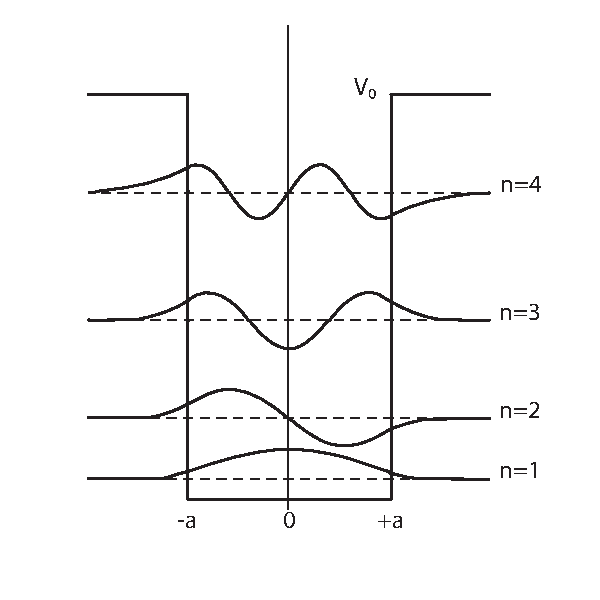
\includegraphics[width=2.2in]{04.root-finding/square_well_energy.pdf}
\caption{A square well potential with depth $V_0$ and width $2a$.  Two symmetric and two anti-symmetric energy eigenstates are plotted.}\label{fig:square_well_energy}
	\end{subfigure}
	\begin{subfigure}{0.45\textwidth}
		\centering
		\includegraphics[width=2.5in]{04.root-finding/square_well_root.pdf}
\caption{The left hand side of Eq (\ref{eq:square_well_symmetric}) is plotted for $z_0=6$. There are two roots. Clearly the root is bracketed by the dashed lines at $x=\frac{\pi}{2}$ and $\frac{3\pi}{2}$.}\label{fig:square_well_root}
	\end{subfigure}
\caption{Quantum particle in a finite suare well}\label{fig:square_well}
\end{figure}

\noindent
\subsection{Classical Turning Points}

In Section  \ref{sec:oscillation1}, we tried to calculate the period of oscillation but we were not quite ready at that time because we did not know how to find the turning points.  Now we can find them using a numerical root finding method. 
Suppose that a particle is bound in a potential
\begin{equation}
U(x) = U_0 \left [ \sin \left ( \frac{2\pi x}{L} \right )- \frac{1}{4} \sin \left ( \frac{4\pi x}{L}\,. \right ) \right ]
\label{eq:ratchet_potential}
\end{equation}
We want to find the period of the bound motion using the formula 
\eqref{eq:oscillation-period}.
The turning points are the roots of $U(x)=E$. The potential is simple and we can find the analytic expression of its derivative.  Hence, the Newton-Raphson method can be used to find the roots.

\vspace{18px}
\noindent
\exercise
Modify Program \ref{prog:newton-secant} and find a pair of the classical turning points of the potential (\ref{eq:ratchet_potential}).
Using the results, find the period of oscillation.

\noindent
\subsection{Closest Approach in Scattering}

In Section \ref{sec:scattering1},
we discussed how to evaluate the scattering angle \eqref{eq:phi_r}.  In order to carry out the integral, we still have to find the closest approach $r_0$ determined by 
Eq. \eqref{eq:root_r}.
For the screened Coulomb potential, we are able to calculate the first order derivative of the equation.  The Newton-Raphson method seems a good choice.

\vspace{18px}
\noindent
\exercise
Solve Eq.  \eqref{eq:root_r} for the Yukawa potential.  Then, calculate the scattering angle, Eq. \eqref{eq:phi_r}, using the method discussed in Section \ref{sec:scattering1}.

\vfill
\noindent
\section{Problems}

\begin{enumerate}[labelwidth=0.5cm,labelindent=0cm,leftmargin=*,label=\bfseries \thechapter.\arabic*,align=left]
\item
The interaction energy between two atoms is often described by the Morse potential\cite{morse_potential}
\begin{equation}
U(r) = D_e \left [\me^{-2 (r-r_0)/a} - 2 \me^{-\alpha (r-r_0)/a} \right ]
\end{equation}
where $r$ is the distance between the atoms.  The parameters, $D_e$. $r_0$, and $a$ are, dissociation energy, equilibrium distance, and the range of interaction, respectively. To simplify numerical calculation, we normalize energy and distance by $D_e$ and $a$. In addition, we use the displacement from the equilibrium position as the coordinate.  Then, the potential is simply
\begin{equation}
U(x) = \me^{-2x}-2 \me^{-x}\,.
\end{equation}
were $x=(r-r_0)/a$.
Find the classical turning points for $E=-0.5$ (This means the actual energy is $E=-D_e/2$ since we use $D_e$ as the unit of energy.)
Do not forget to plot the potential and visually inspect the turning point before using numerical root finding methods.
\item
Find the eigenvalue of all asymmetric state by solving Eq. (\ref{eq:square_well_antisymmetric}) for $z_0=6$.

\item
A quantum ball of mass $m$ is bouncing on a hard floor under a uniform gravity $g$.\cite{qm_bounce}  Schr\"{o}dinger equation for the particle is
\begin{equation}
-\frac{\hbar^2}{2m} \frac{\md^2 \psi(y)}{\md y^2} + m g y\, \psi(y) = E \psi(y).
\label{eq:bouncing_ball}
\end{equation}
The wavefunction $\psi$ must vanish at the floor (boundary condition).  To find the energy eigenvalue, we first simplify the Schr\"{o}dinger equation. Introducing a new variable $z= \alpha (y-E/mg)$ where
\begin{equation}
\alpha = \left ( \frac{2 m^2 g}{\hbar^2} \right )^{1/3}
\end{equation}
Eq. (\ref{eq:bouncing_ball}) is rewritten as
\begin{equation}
\frac{\md^2 \psi(z)}{\md z^2} = z \psi(z)\,
\end{equation}
This equation is known as Airy equation and its solution is Airy function $\text{Ai}(z)$.  Hence, the energy eigenfunction is
$\psi(z) = N\, \text{Ai}(z)$ where $N$ is a normalization constant.  Now, we apply the boundary condition.   At $y=0$. $z=-\alpha E/mg$ and thus $\text{Ai}(-\alpha E/mg)=0$.  This boundary condition indicates that the energy $E$ is determined by the roots of the Airy function. 
Denoting the $n$-th root as $z_n$, the energy is $E_n=- m g z_n /\alpha$.  The bouncing quantum ball has discrete energy!
Find the smallest root of the Airy function and corresponding energy $E_1$.
Use the built-in Airy function $\texttt{airy()}$ in MATLAB.  For C or Fortran, GNU Scientific Library (GSL)\footnote{You can find GSL at 
\texttt{https://www.gnu.org/software/gsl/}.} provides Airy function.
\end{enumerate}

\newpage
\section*{MATLAB Source Codes}
\addcontentsline{toc}{section}{\protect\numberline{}MATLAB Source Codes}


\bigskip\noindent
\program
\label{prog:quad_trick}

\footnotesize
\begin{verbatim}
%**************************************************************************
%*     Example  4.1                                                       *
%*     filename: ch04pr01.m                                               *
%*     program listing number: 4.1                                        *
%*                                                                        *
%*     This program finds roots of a quadratic equation                   *
%*               a x^2 + x + 1/4 = 0                                      *
%*     for which the quadratic equation formula                           * 
%*            x = (-1 + sqrt(1 - a))/(2a)                                 *
%*     fails for small value of a.                                        *
%*                                                                        *
%*     Programed by Ryoichi Kawai for Computational Physics Course.       *
%*     Last modification:  10/13/2013.                                    *
%**************************************************************************
clear all;

b=1;  % fixed parameters
c=0.25;

n=1;
a(1)=1;
while (a>eps())
  d = b^2-4*a(n)*c;
  x1(n) = (-b+sqrt(d))/(2*a(n));
  x2(n) = -2*c/(b+sqrt(d));
  fprintf('a= %22.16e, lhs=%22.16e, rhs=%22.16e \n',a(n),x1(n),x2(n));
  n=n+1;
  a(n)=a(n-1)/10;
end

% plot the results
p=loglog(a(1:n-1),abs(x2+0.25),'o',a(1:n-1),abs(x1+0.25),'s');
set(p(1),'Linewidth',2,'Color','red')
set(p(2),'Linewidth',2,'Color','blue')
xlabel('a','Fontsize',14)
ylabel(texlabel('|x - x_0|'),'Fontsize',14)  % x_0 = root at a=0
legend('lhs','rhs')
legend('Location','Southeast')
\end{verbatim}
\normalsize

\ruleend

\bigskip\noindent
\program
\label{prog:roots_cubic}
\footnotesize
\begin{verbatim}
%**************************************************************************
%*     Example  4.2                                                       *
%*     filename: ch04pr02.m                                               *
%*     program listing number: 4.2                                        *
%*                                                                        *
%*     This program finds roots of a cubic equation                       *
%*               a*x^3 + b*x^2 + c*x + d = 0                              *
%*                                                                        *
%*     Programed by Ryoichi Kawai for Computational Physics Course.       *
%*     Last modification:  10/13/2013.                                    *
%**************************************************************************
clear all;

% coefficients
b=-9; c=23; d=-15;

% formula for cubic polynomials
F=(3*c-b^2)/3;
G=(2*b^3 - 9*b*c + 27*d)/27;
H=G^2/4 + F^3/27;

yes = false;

if H>0
    S= (sqrt(H)-G/2)^(1./3.);
    U=-(sqrt(H)+G/2)^(1./3.);
    x = S+U-b/3;
    fprintf('Answer = %.5f\n',x);

else
    I=sqrt(G^2/4-H);
    J=I^(1./3.);
    K=acos(-G/(2*I));
    M=cos(K/3);
    N=sqrt(3)*sin(K/3);
    P=-b/3;    
    x(1) = P-J*(M+N);
    x(2) = P-J*(M-N);
    x(3) = P+2*J*M;
    fprintf('Answer = %.5f,  %.5f,  %.5f \n',x);
end
\end{verbatim}
\normalsize

\ruleend

\program
\bigskip\noindent
\label{prog:bisection}
\footnotesize
\begin{verbatim}
%**************************************************************************
%*     Example  4.3                                                       *
%*     filename: ch04pr03.m                                               *
%*     program listing number: 4.3                                        *
%*                                                                        *
%*     This program finds roots of a cubic equation                       *
%*               a*x^3 + b*x^2 + c*x + d = 0                              *
%*     using the bisection method.                                        *
%*                                                                        *
%*     Programed by Ryoichi Kawai for Computational Physics Course.       *
%*     Last modification:  01/24/2018.                                    *
%**************************************************************************
clear all;

% define a cubic equation
b = -9;
c = 23;
d =-15;

f = @(x) x^3+b*x^2+c*x+d;

% tolerance
epsilon=input('Enter tolerance =');

% initial bracket
x1=1.5;
x2=4;
f1 = f(x1);
f2 = f(x2);

% iteration counter
n=0;

% mid point
xm = (x1+x2)/2;
fm = f(xm);
while abs(fm) > epsilon
    if f1*fm < 0  % root in the lower half
        x2=xm;
        f2=fm;
    else          % root in the upper half
        x1=xm;
        f1=fm;
    end
    xm = (x1+x2)/2;  % new mid point
    fm = f(xm);
    n=n+1;
end

fprintf('Answer = %.5f  (iteration= %i)\n',xm,n);
\end{verbatim}

\normalsize


\ruleend

\bigskip\noindent
\program
\label{prog:newton-secant}
\footnotesize
\begin{verbatim}
%**************************************************************************
%*     Example 4.4                                                        *
%*     filename: ch04pr04.m                                               *
%*     program listing number: 4.4                                        *
%*                                                                        *
%*     This program seeks the root of                                     *
%*             cos(3*x)*sin(x)=0                                          *
%*     between x=0.2 and 0.8 using bisection, Newton-Raphson, and         *
%*     secant methods.                                                    *
%*                                                                        *
%*     Programed by Ryoichi Kawai for Computational Physics Course        *
%*     Revised on 01/07/2014.                                             *
%**************************************************************************
clear all;

% define function and its derivative
f=@(x) cos(3*x)*sin(x);
df=@(x) -3*sin(3*x)*sin(x) + cos(3*x)*cos(x);

% initial bracket
x1=0.2;
x2=0.8;
f1=f(x1);
f2=f(x2);
if f1*f2 > 0
   error('Bracket is incorrect');
end

% tolerance
epsilon=1e-8;

% bisection 10 iterations

% iteration counter
n=0;

% Bisection method (10 iterations)
xm = (x1+x2)/2;
fm = f(xm);
while n<10
    if f1*fm < 0  % root in the lower half
        x2=xm;
        f2=fm;
    else          % root in the upper half
        x1=xm;
        f1=fm;
    end
    xm = (x1+x2)/2;  % new mid point
    fm = f(xm);
    n=n+1;
end

fprintf('Bisection      = %.8f  (iteration= %i)\n',xm,n);

% Newton-Raphson method
x = xm;
fx = fm;
n = 0;
while abs(fx)> epsilon
    dfx = df(x);
    x = x - fx/dfx;
    fx = f(x);
    n = n+1;
end

fprintf('Newton-Raphson = %.8f  (iteration= %i)\n',x,n);

% Secant method
dx = (x2-x1)/10;
x1 = xm;
f1 = fm;
x2 = x1 + dx;
f2 = f(x2);
n = 0;
while abs(f2)> epsilon
    x = x2 - (x2-x1)/(f2-f1)*f2;
    x1 = x2;
    f1 = f2;
    x2 = x;
    f2 = f(x);
    n = n+1;
end

fprintf('Secant         = %.8f  (iteration= %i)\n',x,n);
\end{verbatim}
\normalsize

\ruleend

\bigskip\noindent
\program
\label{prog:ising}
\footnotesize
\begin{verbatim}
%**************************************************************************
%*     Example 4.5                                                        *
%*     filename: ch04pr05.m                                               *
%*     program listing number: 4.5                                        *
%*                                                                        *
%*     This program calculates magnetization as a function of             *
%*     temperature using the mean field Ising model:                      *
%*         x = x tan(x/S)                                                 *
%*     where the variables are normalized as                              *
%*         x = m/m_0 and S=k*T/(C*m_0) .                                  *
%*                                                                        *
%*     Programed by Ryoichi Kawai for Computational Physics Course        *
%*     Revised on 01/07/2014.                                             *
%**************************************************************************
clear all;
N=101; % number of data points
tol=10^(-6);  % tolerance

dS = 2/(N-1); % step size in temperature

for i=1:N
    S=(i-1)*dS;  % temperature
    a=1/S;
    f=@(x) x - tanh(a*x);  % function
    df=@(x) 1 - a*sech(a*x)^2;  % derivative
    % Newton-Raphson method
    x=2;  % initial guess
    fx=f(x);
    while fx>tol
      x=x-fx/df(x);
      fx=f(x);
    end
    % store the magnetization and temperature  
    m(i)=x;
    t(i)=S;
end

p=plot(t,m,t,-m,[0,1],[0,0]);
xlabel('T','fontsize',14);
ylabel('m','fontsize',14);
set(p(1),'linewidth',2,'color','blue');
set(p(2),'linewidth',2,'color','blue');
set(p(3),'linewidth',2,'color','red');
axis([0 2 -1.1 1.1]);
\end{verbatim}
\normalsize

\ruleend

\bigskip\noindent
\program(a)
\label{prog:square_well}
\footnotesize
\begin{verbatim}
%**************************************************************************
%*     Secion 4.6.                                                        *
%*     filename: ch04pr06.m                                               *
%*     program listing number: 4.6(a)                                     *
%*                                                                        *
%*     Require: rootfinding.m                                             *
%*                                                                        *
%*     This program finds trhe energy eigenvalues of a pqrticle           *
%*     in a finite square well potential using the secant root            *
%*     finding methods.                                                   *
%*                                                                        *
%*     Programed by Ryoichi Kawai for Computational Physics Course        *
%*     Revised on 01/07/2014.                                             *
%**************************************************************************
clear all;

z0=6;  %system parameter

f=@(z) z*tan(z) - sqrt(z0*z0-z*z);  %define function

%control parameters
N=100;
K=ceil(z0/pi);  %The number of roots

% initial bracket
z1=0;
z2=pi/2;

for k=1:K   
    dz = (z2-z1)/N;  % small shit
    z = rootfinding(f,z1+dz,z2-dz,10,10^(-6));
    fprintf('root=%.8f\n',z);
    z1 = z2;
    z2 = min([z0,z1 + pi]);
end
\end{verbatim}
\normalsize

\medskip\noindent
\program(b)
\footnotesize
\begin{verbatim}
%**************************************************************************
%*     Secion 4.6.                                                        *
%*     filename: rootfinding.m                                            *
%*     program listing number: 4.6(b)                                     *
%*                                                                        *
%*     Inputs                                                             *
%*         f = function name                                              *
%*         x1, x2 = bracket                                               *
%*         N = interations of bisection                                   *
%*         tol = tolerance for scant method                               *
%*     Output:                                                            *
%*         x = root                                                       *
%*                                                                        *
%*     This program find a root of a given funcion f(x)=0                 *
%*     using the bisection and secant root finding method                 *
%*     finding methods.                                                   *
%*                                                                        *
%*     Programed by Ryoichi Kawai for Computational Physics Course        *
%*     Revised on 01/07/2014.                                             *
%**************************************************************************

function x=rootfinding(f,x1,x2,N,tol)

% check if the initial bracket satisfies the necessary condition.
f1=f(x1);
f2=f(x2);
if f1*f2 > 0
   error('Bracket is incorrect');
   display(x1,x2,f1,f2);
end

% Bisection method (N iteration)
n=0; % iteration counter

% mid point
xm = (x1+x2)/2;
fm = f(xm);
n=0;

while n<N
    if f1*fm < 0  % root in the lower half
        x2=xm;
        f2=fm;
    else          % root in the upper half
        x1=xm;
        f1=fm;
    end
    xm = (x1+x2)/2;  % new mid point
    fm = f(xm);
    n=n+1;
end

% Secant method
dx = (x2-x1)/10;
x1 = xm;
f1 = fm;
x2 = x1 + dx;
f2 = f(x2);
n = 0;
while abs(f2)> tol
    x = x2 - (x2-x1)/(f2-f1)*f2;
    x1 = x2;
    f1 = f2;
    x2 = x;
    f2 = f(x);
    n = n+1;
end
\end{verbatim}
\normalsize


\section*{Python Source Codes}
\addcontentsline{toc}{section}{\protect\numberline{}Python Source Codes}
\setcounter{program}{0}

\bigskip\noindent
\program
\footnotesize
\begin{verbatim}
#!/usr/bin/env python3
"""
%**************************************************************************
%*     Example  4.1                                                       *
%*     filename: ch04pr01.py                                              *
%*     program listing number: 4.1                                        *
%*                                                                        *
%*     This program finds roots of a quadratic equation                   *
%*               a x^2 + x + 1/4 = 0                                      *
%*     for which the quadratic equation formula                           * 
%*            x = (-1 + sqrt(1 - a))/(2a)                                 *
%*     fails for small value of a.                                        *
%*                                                                        *
%*     Programed by Ryoichi Kawai for Computational Physics Course.       *
%*     Last modification:  01/07/2017.                                    *
%**************************************************************************
"""
import numpy as np
import matplotlib.pyplot as plt

b=1.0
c=0.25
a=1.0
x=np.zeros(50)
y1=np.zeros(50)
y2=np.zeros(50)
n=0
while a > np.finfo(float).eps:
    x[n]=a
    d=b**2-4*a*c
    y1[n]=(-b+np.sqrt(d))/(2.0*a)
    y2[n]=-2*c/(b+np.sqrt(d))
    print("a={0:22.16e}, regular={1:22.16e}, smart={2:22.16e}"
          .format(x[n],y1[n],y2[n]))
    n+=1
    a=a/10.

plt.ioff()
plt.figure(figsize=(6,5))
plt.loglog(x[0:n],abs(y2[0:n]+0.25), 'ob', label='smart')
plt.loglog(x[0:n],abs(y1[0:n]+0.25), 'or', label='regular')
plt.legend(loc=4)
plt.xlabel('a')
plt.ylabel('x')
plt.show()
\end{verbatim}
\normalsize

\ruleend

\bigskip\noindent
\program
\footnotesize
\begin{verbatim}
#!/usr/bin/env python3
# -*- coding: utf-8 -*-
"""
%**************************************************************************
%*  Example  4.2                                                          *
%*  filename: ch04pr02.py                                                 *
%*  program listing number: 4.2                                           *
%*                                                                        *
%*     This program finds roots of a cubic equation                       *
%*               a*x^3 + b*x^2 + c*x + d = 0                              *
%*                                                                        *
%*     Programed by Ryoichi Kawai for Computational Physics Course.       *
%*     Last modification:  01/14/2017.                                    *
%**************************************************************************
"""
import numpy as np
# coefficients
b=-9.0; c=23.0; d=-15.0
k=0

# formula for cubic polynomials
F=(3.0*c-b**2)/3.0
G=(2.0*b**3 - 9.0*b*c + 27.0*d)/27.0
H=G**2/4.0 + F**3/27.0

yes = False

if H>0.0:
    S= (np.sqrt(H)-G/2.0)**(1./3.)
    U=-(np.sqrt(H)+G/2.0)**(1./3.)
    x1 = S+U-b/3.0
    print("Answer = {0:10.5f}".format(x1))

else:
    I=np.sqrt(G**2/4.0-H)
    J=I**(1./3.)
    K=np.arccos(-G/(2.0*I))
    M=np.cos(K/3.0)
    N=np.sqrt(3)*np.sin(K/3.0)
    P=-b/3.0
    x3=np.zeros(3)    
    x3[0] = P-J*(M+N)
    x3[1] = P-J*(M-N)
    x3[2] = P+2.0*J*M
    print("Answer = {0:10.5f}, {1:10.5f}, {2:10.5f}"
          .format(x3[0],x3[1],x3[2]))
\end{verbatim}
\normalsize

\ruleend

\bigskip\noindent
\program
\footnotesize
\begin{verbatim}
#!/usr/bin/env python3
# -*- coding: utf-8 -*-
"""
%**************************************************************************
%*     Example  4.3                                                       *
%*     filename: ch04pr03.m                                               *
%*     program listing number: 4.3                                        *
%*                                                                        *
%*     This program finds roots of a cubic equation                       *
%*               a*x^3 + b*x^2 + c*x + d = 0                              *
%*     using the bisection method.                                        *
%*                                                                        *
%*     Programed by Ryoichi Kawai for Computational Physics Course.       *
%*     Last modification:  10/13/2013.                                    *
%**************************************************************************
"""
import numpy as np

# define a cubic equation
def f(x):
    return x**3-9.0*x**2+23.0*x-15

if __name__ == "__main__": 
    
    tol=input("Enter tolerance =")  # Read a tolerabce from the console
    epsilon=np.float(tol)
    
    # initial bracket
    x1=1.5
    x2=4.0
    f1 = f(x1)
    f2 = f(x2)

    # iteration counter
    n=0

    # mid point
    xm = (x1+x2)/2.0
    fm = f(xm)
    
    while x2-x1 > epsilon:
        if f1*fm < 0:  # root in the lower half
            x2=xm
            f2=fm
        else:          # root in the upper half
            x1=xm
            f1=fm

        xm = (x1+x2)/2.0      # new mid point
        fm = f(xm)
        n+=1

    print("Answer = {0:7.5f}, (iteration = {1:3d})"
          .format(xm,n))
\end{verbatim}
\normalsize

\ruleend

\bigskip\noindent
\program
\footnotesize
\begin{verbatim}
#!/usr/bin/env python3
# -*- coding: utf-8 -*-
"""
%**************************************************************************
%*     Example 4.4                                                        *
%*     filename: ch04pr04.m                                               *
%*     program listing number: 4.4                                        *
%*                                                                        *
%*     This program seeks the root of                                     *
%*             cos(3*x)*sin(x)=0                                          *
%*     between x=0.2 and 0.8 using bisection, Newton-Raphson, and         *
%*     secant methods.                                                    *
%*                                                                        *
%*     Programed by Ryoichi Kawai for Computational Physics Course        *
%*     Revised on 01/14/2017.                                             *
%**************************************************************************
"""
import sys
import numpy as np

# define function and its derivative
def f(x):
    return np.cos(3.0*x)*np.sin(x)

def df(x):
    return -3.0*np.sin(3*x)*np.sin(x) + np.cos(3.0*x)*np.cos(x);

if __name__ == "__main__": 
    # initial bracket
    x1, x2 = input("Initial blacket (a pair o numbers) = ").split()
    x1, x2 = [np.float(x1), np.float(x2)]
    
    f1=f(x1)
    f2=f(x2)
    if f1*f2 > 0:
        sys.exit('Bracket is incorrect')
        
    # tolerance
    epsilon = input("Tolerance = ")
    epsilon = np.float(epsilon)

    # bisection 10 iterations
    n=0 # iteration counter

    xm = (x1+x2)/2.0
    fm = f(xm)
    
    while n<10:
        if f1*fm < 0:  # root in the lower half
            x2=xm
            f2=fm
        else:          # root in the upper half
            x1=xm
            f1=fm

        xm = (x1+x2)/2.0  # new mid point
        fm = f(xm)
        n+=1

    print("Bisection      = {0:12.8f}  (iteration= {1:4d})"
          .format(xm,n))

    # Newton-Raphson method
    x = xm
    fx = fm
    n = 0
    while abs(fx)> epsilon:
        dfx = df(x)
        x = x - fx/dfx
        fx = f(x)
        n+=1

    print("Newton-Raphson = {0:12.8f}  (iteration=  {1:4d})"
          .format(x,n))

    # Secant method
    dx = (x2-x1)/10.
    x1 = xm
    f1 = fm
    x2 = x1 + dx
    f2 = f(x2)
    n = 0
    while abs(f2)> epsilon:
        x = x2 - (x2-x1)/(f2-f1)*f2
        x1 = x2
        f1 = f2
        x2 = x
        f2 = f(x)
        n+=1

    print("Secant         = {0:12.8f}  (iteration=  {1:4d})"
          .format(x,n))
\end{verbatim}
\normalsize

\ruleend

\bigskip\noindent
\program
\footnotesize
\begin{verbatim}
#!/usr/bin/env python3
# -*- coding: utf-8 -*-
"""
%**************************************************************************
%*  Example 4.5                                                           *
%*  filename: ch04pr05.py                                                 *
%*  program listing number: 4.5                                           *
%*                                                                        *
%*     This program calculates magnetization as a function of             *
%*     temperature using the mean field Ising model:                      *
%*         x = x tan(x/S)                                                 *
%*     where the variables are normalized as                              *
%*         x = m/m_0 and S=k*T/(C*m_0) .                                  *
%*                                                                        *
%*     Programed by Ryoichi Kawai for Computational Physics Course        *
%*     Revised on 01/14/2017.                                             *
%**************************************************************************
"""
import numpy as np
import matplotlib.pyplot as plt

def f(x,a):
    return x - np.tanh(a*x)

def df(x,a):
    return 1.0 - a/np.cosh(a*x)**2

if __name__ == "__main__": 
    N=100 # number of data points
    tol=1.0e-6  # tolerance

    m=np.zeros(N+1)
    t=np.zeros(N+1)
    dS = 2.0/N   # step size in temperature

    
    for k in range(0,N):
        S=(k+1)*dS  # temperature
        a=1.0/S
        # Newton-Raphson method
        x=2.0    # initial guess
        fx=f(x,a)
        while fx>tol:
            x=x-fx/df(x,a)
            fx=f(x,a)

        # store the magnetization and temperature  
        m[k]=x
        t[k]=S

    plt.ioff()
    plt.figure(figsize=(12,5))
    plt.plot(t,m, '-r')
    plt.plot(t,-m, '-r')
    plt.plot([0,1],[0,0],'--w')
    plt.ylim([-1.2,1.2])
    plt.xlabel('T')
    plt.ylabel('m')
    plt.savefig('ch04r05.pdf')
    plt.show()
\end{verbatim}
\normalsize

\ruleend

\bigskip\noindent
\program (a)
\footnotesize
\begin{verbatim}
#!/usr/bin/env python3
# -*- coding: utf-8 -*-
"""
%**************************************************************************
%*  Secion 4.6.                                                           *
%*  filename: ch04pr06.py                                                 *
%*  program listing number: 4.6-1                                         *
%*                                                                        *
%*     Require: rootfinding.py                                            *
%*                                                                        *
%*     This program finds trhe energy eigenvalues of a pqrticle           *
%*     in a finite square well potential using the secant root            *
%*     finding methods.                                                   *
%*                                                                        *
%*     Programed by Ryoichi Kawai for Computational Physics Course        *
%*     Revised on 01/07/2014.                                             *
%**************************************************************************
"""

import numpy as np
import rootfinding as rf

def f(z):
    global z0
    return z*np.tan(z) - np.sqrt(z0*z0-z*z)

if __name__ == "__main__":
    global z0
    z0=6  #system parameter
    #control parameters
    N=100
    K=np.int(np.ceil(z0/np.pi))  #The number of roots

    # initial bracket
    z1=0.0;
    z2=np.pi/2.0

    for k in range(1,K+1):  
        dz = (z2-z1)/N  # small shit
        z = rf.findaroot(f,z1+dz,z2-dz,10,1.0e-6)
        print("root={0:12.8f}".format(z))
        z1 = z2
        z2 = min([z0,z1 + np.pi])

\end{verbatim}
\normalsize

\bigskip\noindent
\program (b)
\footnotesize
\begin{verbatim}
#!/usr/bin/env python3
# -*- coding: utf-8 -*-
"""
%**************************************************************************
%*   Secion 4.6.                                                          *
%*   filename: rootfinding.py                                             *
%*   program listing number: 4.6-2                                        *
%*                                                                        *
%*     Inputs                                                             *
%*         f = function name                                              *
%*         x1, x2 = bracket                                               *
%*         N = interations of bisection                                   *
%*         tol = tolerance for scant method                               *
%*     Output:                                                            *
%*         x = root                                                       *
%*                                                                        *
%*     This program find a root of a given funcion f(x)=0                 *
%*     using the bisection and secant root finding method                 *
%*     finding methods.                                                   *
%*                                                                        *
%*     Programed by Ryoichi Kawai for Computational Physics Course        *
%*     Revised on 01/07/2014.                                             *
%**************************************************************************
"""
def findaroot(f,x1,x2,N,tol):
    
    f1=f(x1)
    f2=f(x2)
    if f1*f2 > 0:
        exit('Bracket is incorrect')

    # Bisection method (N iteration)
    n=0  # iteration counter

    # mid point
    xm = (x1+x2)/2.0
    fm = f(xm)

    while n<N+1:
        if f1*fm < 0.0:  # root in the lower half
            x2=xm
            f2=fm
        else:            # root in the upper half
            x1=xm
            f1=fm

        xm = (x1+x2)/2.0  # new mid point
        fm = f(xm)
        n+=1

    # Secant method
    dx = (x2-x1)/10.0
    x1 = xm
    f1 = fm
    x2 = x1 + dx
    f2 = f(x2)
    n = 0
    while abs(f2)> tol:
        x = x2 - (x2-x1)/(f2-f1)*f2
        x1 = x2
        f1 = f2
        x2 = x
        f2 = f(x)
        n+=1

    return x
\end{verbatim}
\normalsize

\ruleend
\vfill

\newpage
%\bibliography{compphys}
\bibliographystyle{unsrt}
\bibliography{compphys}

\vfill
\chapter{Ordinary Differential Equations I:\\ {Initial Value Problems}}\label{ch:ode1}
 
Many physics theories are expressed in various forms of ordinary differential equation(ODE). 
For example, Newton's equations of motion are written in ODE.  In classical mechanics courses, we solve various example problems analytically.  In practice, however, the majority of problems cannot be solved analytically because Newton's equations are non-linear except for simple harmonic oscillators.  The motion of a planet (Kepler problem) is a very special case where analytical solution is possible despite of the non-linearity. We must resort to numerical methods for almost all practical problems.

An ODE generally allows infinitely many different solutions. We want to find a solution that matches to given conditions  ODE alone cannot pick it.  It is boundary conditions that determine a specific solution.  In physics there are two types of problems.  When we want to find a time evolution of physical quantities, we solve ODEs with initial conditions.  Initial conditions are a kind of boundary condition given at a single point (initial time).  On the other hand, when we want to know a spatial profile of physical quantities, we usually specify conditions at two different points.  Eigenvalue problems expressed in differential equation forms belong to the latter type of boundary conditions.  The former is called initial value problem and the latter boundary value problem.  In numerical calculation, these two problems are quite different.  In this chapter we focus on initial value problems, boundary value problems are discussed in next chapter and eigenvalue problems in the following chapter. 


\section{Standard forms of Initial Value Problems in Physics}
 
A typical initial value problem in physics is a first order ODE expressed in a standard form,
\begin{equation}
\dot{x} = F(x,t) 
\label{eq:ode1st}
\end{equation}
or a set of second order ODEs
\begin{equation}
\ddot{x} = F(x,\dot{x},t)
\end{equation}
where $x$ is a function of time.
The functions $x$ and $F$ can be vector. For example, Newton's equation of motion 
\begin{equation}\label{eq:newton-eom}
\ddot{\mathbf{r}} = \frac{1}{m} \mathbf{F}(\mathbf{r},\mathbf{v},t).
\end{equation}
is a standard second order ODE with $\mathbf{r}=\{x,y,z\}$, and $\mathbf{F}=\{F_x,F_y,F_z\}$.  In other words, Eq. \eqref{eq:newton-eom} is a set of coupled ODEs.
In general, the second order ODEs of this kind can be transformed to another set of first order ODEs. Therefore, numerical methods for the first order ODEs can be used to solve the second order ODEs as well.  However, there are also algorithms specific to the second order ODEs such as the Verlet argorithm, which can be more efficient in certain applications.

\section{First Order Differential Equations}
 
For simplicity, we focus on the first order ODE of a single variable $x$ for a while. Multivariable cases will be discussed at the end of this section. More specifically, we want to solve the following type of ODE:
\begin{equation}\label{eq:ode-1d}
\dot{x} = F(x,t)
\end{equation}
for a given initial condition $x(t_0)$ and a function $F(x,t)$.  The exact solution is a continuous function $x(t)$ for time period from an initial time $t_0$ to a final time $t_F$.  However, in the computer we work with discrete time $t_n = t_0 + n h,\, n=0, \cdots, N$ where $h$ is a time step defined by $h=\displaystyle\frac{t_F-t_0}{N}$.  The numerical solution is obtained as a sequence $x(t_0), x(t_1), x(t_2), \cdots, x(t_N)$.  Our goal is to develop numerical algorithms to predict $x(t_{n+1})$  knowing the previous points $x(t_n), x(t_{n-1}), \cdots x(t_0)$. We can construct the whole sequence by repeating the procedure. In the following subsections, we use simplified expressions, $x_n=x(t_n)$ and $F_n = F(x(t_n),t_n)$. 

To begin with, we convert the ODE \eqref{eq:ode-1d} to a recursive equation involving an integral.  Integrating Eq. \eqref{eq:ode-1d} from $t_n$ to $t_{n+1}$, we obtain
\begin{equation}\label{eq:ode-integral}
x_{n+1} = x_n + \int_{t_n}^{t_{n+1}} F[x(t),t]\, \dd{t}\, .
\end{equation}
This expression is still mathematically exact.  However, 
it is not a solution since the integrand depends on the continuous solution $x(t)$ which we don't know.  How can we evaluate the integral without knowing $x(t)$ for $t_n < t < t_{n+1}$? Nonetheless our numerical methods are derived from this recursive equation.  

\subsection{Euler Method}\label{sec:Euler}

\begin{figure}
	\begin{subfigure}{0.45\textwidth}
		\centering
		\includegraphics[width=2.5in]{05.ode1/euler-integral.pdf}
\caption{The curve in the figure represents the integrand of Eq. (\ref{eq:ode-integral}), which is unknown to us. Knowing $F_n$ and $h$, we approximate the integral by the rectangular rule.  The unaccounted area is proportional to $h^2$.}
\label{fig:euler-integral}
	\end{subfigure}
	\begin{subfigure}{0.45\textwidth}
		\centering 
		\includegraphics[width=2.5in]{05.ode1/euler-x.pdf}
\caption{Using the slope of the curve $F_n$,  we extrapolate next point $x_{n+1}$ assuming the curve is close to a straight line within a small step $h$.}
\label{fig:euler-x}
\end{subfigure}
\caption{Illustration of the Euler method}
\label{fig:euler-rule}
\end{figure}

Now, we try to estimate the integral in Eq.  \eqref{eq:ode-integral} only with known values $x_n$ and $F_n$.
Figure \ref{fig:euler-integral} shows what we are trying to do. Recalling that the rectangle rule of numerical integration depends only on the single point [see Eq. \eqref{eq:fwd-rectangle}], we use the rectangular rule to approximate the integral in Eq. \eqref{eq:ode-integral}:
\begin{equation}\label{eq:ode-rectangular}
\int_{t_n}^{t_{n+1}} F[x(t),t] \dd{t} \approx F_n\, h
\end{equation}
which leads to the Euler method:
\begin{equation}\label{eq:euler-rule}
\fbox{$x_{n+1} = x_n + F_n\, h$}.
\end{equation}


Starting from the initial value, $x_0$, we first evaluate $F_0=F(x_0,t_0)$.  Then, we obtain $x_1$ by Eq. ({eq:euler-rule}).
Using this procedure recursively, we obtain the whole sequence from $x_0$ to $x_N$.

\bigskip 
\begin{myalgobox}
	\Algorithm{Euler method}\label{algo:euler}
	
	\medskip
	\begin{minipage}{5.5in}
		\begin{enumerate}
			\item Set the total period $T$ and the number of steps $N$.
			\item Calculate the step size $h=\displaystyle\frac{T}{N}$.
			\item Set the initial condition $x_0=0$ and $t_0=0$.
			\item Reset the counter: $n=0$.
			\item Repeat the following $N$ times
			\item Evaluate the function $F_n=F(x_n,t_n)$.
			\item Calculate a new point $x_{n+1}=x_n+F_n h$.
			\item Increment the step: $n=n+1$.
			\item Go to Step 6.
		\end{enumerate}
	\end{minipage}
\end{myalgobox}
	
\bigskip
	
The area omitted in Fig. \ref{fig:euler-integral})
is order of $h^2$.  Therefore the local error of the Euler method is the order of $h^2$. After $N$ iteration, the global error becomes $N h^2 \sim \order{h}$.  If $h$ is small enough, we hope that this is a good approximation. In practice, the Euler method is not good enough for most applications.


\subsection{Predictor-Corrector Method}

The higher order of error in the Euler method  is due to the inaccuracy of the rectangle rule \eqref{eq:ode-rectangular} (See Chapter \ref{ch:integrals}).
We expect that the trapezoidal rule 
\begin{equation}\label{eq:ode-trapezoidal}
    \int_{t_n}^{t_{n+1}} F[x(t),t]\dd{t}\approx \frac{(F_n + F_{n+1}) h}{2}
\end{equation}
provides a better estimate of the integral in (\ref{eq:ode-integral}).
Then, Eq. \eqref{eq:ode-integral} becomes
\begin{equation}\label{eq:ode-implicit}
x_{n+1} = x_n + \frac{h}{2}
\left[ F(x_n,t_n) + F(x_{n+1},t_n+h) \right] + \order{h^3}.
\end{equation}
This expression is 	implicit with respect to $x_{n+1}$ since the right hand side also depends on it.
To find $x_{n+1}$, we must use a root-finding method,
which is in principle possible but too time-consuming for practical applications.  A better way is to use an approximate value of $x_{n+1}$ in the right hand side. We \emph{predict} $x_{n+1}$ using the Euler method and then \emph{correct} it by Eq. \eqref{eq:ode-implicit}.  This is the "predictor-corrector" method.  The above procedure is summarized in Algorithm \ref{algo:predictor-corrector}, which looks different from the above method but more convenient when you write a program.

\bigskip

\begin{myalgobox}
	\Algorithm{Predictor-corrector method}\label{algo:predictor-corrector}
		
	\medskip
	\begin{minipage}{5.5in}
		\begin{enumerate}
			\item Set the total period $T$ and the number of steps $N$.
			\item Calculate the step size $h=\displaystyle\frac{T}{N}$.
			\item Set the initial condition $x_0=0$ and $t_0=0$.
			\item Reset the counter: $n=0$.
			\item Repeat the following $N$ times.
			\item Increment time: $t_{n+1}=t_0 + (n+1)h$.
			\item Predictor: $k_1 = F(x_n,t_n)$						
			\item Corrector: $k_2 = F(x_n+k_1 h,t_{n+1}) $.
			\item New point: $x_{n+1}=x_n + \displaystyle\frac{h}{2} \left ( k_1 + k_2 \right )$.
			\item Increment the step: $n=n+1$.
			\item Go to Step 6.
		\end{enumerate}
	\end{minipage}
\end{myalgobox}


\bigskip
The above algorithm uses the Euler method as predictor. The local order of the error $\order{h^3}$ is better than that of the Euler method. Therefore, the corrector works.   Figure \ref{fig:predict-correct} illustrates the improvement. However, even higher accuracy can be attained if a better method such as the Adams-Bashforth method is used as predictor and a higher order corrector is used. See Ref. \cite{numerical_recipes} for the detailed description of advanced predictor-corrector methods.


\begin{figure}
	\begin{subfigure}{0.45\textwidth}
		\centering
		\includegraphics[height=2.5in]{05.ode1/predict-correct-integral.pdf}
\caption{$F_{n+1}$ is linearly extrapolated from two previous points $F_{n-1}$ and $F_n$.  Then, trapezoidal rule is used to integrate.}
\label{fig:predict-correct-integral}
	\end{subfigure}
	\begin{subfigure}{0.45\textwidth}
		\centering 
		\includegraphics[height=2.5in]{05.ode1/predict-correct-x.pdf}
\caption{The linear extrapolation in the left panel is equivalent to assume that the change of the slope ($\Delta$) is the same as that in the previous step.}
\label{fig:predict-correct-rule}
	\end{subfigure}
\caption{Illustration of the Predictor-Corrector Method}\label{fig:predict-correct}
\end{figure}

\bigskip
\begin{example}[Free Falling] \label{ex:free_falling1}

\medskip
A particle of $1\, kg$ is dropped from rest in uniform gravity $9.8\, m/s^2$.  The drag force due to the presence of air is $-\gamma v$ where $v$ is velocity and the frictional coefficient is $\gamma=1.0\, kg/s$. The equation of motion is given by
\begin{equation}
m \dot{v} = - \gamma v - m g
\end{equation}
ans its solution is 
\begin{equation}
v(t) = \frac{m g}{\gamma} \left ( \me^{-\gamma t} -1 \right )\,.
\end{equation}
Let us integrate the Newton equations using Euler and Predictor-Corrector methods. Program \ref{prog:freefalling1} implements the methods.  We integrate from $t=0$ to $t=10$ using the step size $h=0.01$.  In Fig. \ref{fig:free_falling1}, the results of the two methods and the exact solution are plotted.  From naked eyes, there is no difference between them.  However, if look at the absolute errors (right panel), the difference is clear. The predictor-corrector method is much better.  Note also that the error increases at the beginning where the velocity changes very rapidly and decreases as the velocity approaches the terminal value.

\begin{figure}
\centerline{\includegraphics[height=2.5in]{05.ode1/free_falling1.pdf}}
\caption{Output of Example \ref{ex:free_falling1}.  The left panel shows the velocity as a function of time.  All three lines look identical. The right panel shows the absolute errors. The error in the predictor-corrector method is clearly  square of the error in the Euler method.}
\label{fig:free_falling1}
\end{figure}
\end{example}

\noindent
\subsection{2nd-Order Runge-Kutta Method}\label{sec:Runge-Kutta}

\begin{figure}
	\begin{subfigure}{0.45\textwidth}
		\centering
		\includegraphics[height=2.5in]{05.ode1/runge-integral.pdf}
\caption{Using the Euler method, $F_{n+1/2}$ is estimated. Then, the integral is approximated by the area of the rectangle.}
\label{fig:runge-integral}
	\end{subfigure}
	\begin{subfigure}{0.45\textwidth}
		\centering 
		\includegraphics[height=2.5in]{05.ode1/runge-x.pdf}
\caption{The slop at the mid point ($k_2$) is estimate by the Euler method . Then the new point is predicted with the same slope (red line).}
\label{fig:runge-x}
	\end{subfigure}
\caption{Illustration of the second order Runge-Kutta Method.}
\label{fig:runge-kutta-rule}
\end{figure}

If the value of $x$ at the mid point between $x_n$ and $x_{n+1}$ 
is available, the higher
accuracy may be obtained. The integral in Eq 
\eqref{eq:ode-integral} can be evaluated by a single point (see Fig. \ref{fig:runge-kutta-rule}.):
\begin{equation}\label{eq:ode-integral-mid}
\int_{t_n}^{t_{n+1}} F(x(t),t) dt = h F_{n+1/2}.
 + \order{h^3}
\end{equation}
where $F_{n+1/2} \equiv F[]x(t_n+1/2),t_n + h/2]$, which is still unknown to us. 
We estimate it using the Euler method and obtain
\begin{equation}
x_{n+1/2} = x_n + \frac{h}{2} F_n
\label{eq:runge-mid}
\end{equation}
which enables us to compute $F_{n+1/2}$ in Eq. (\ref{eq:ode-integral-mid}). This is the second-order Runge-Kutta method. 

\bigskip
\begin{myalgobox}
	\Algorithm{Second-order Runge-Kutta method}\label{algo:runge-kutta2}

	\medskip	
	\begin{minipage}{5.5in}
		\begin{enumerate}
			\item Set the total period $T$ and the number of steps $N$.
			\item Calculate the step size $h=\displaystyle\frac{T}{N}$.
			\item Set the initial condition $x_0=0$ and $t_0=0$.
			\item Reset the counter: $n=0$.
			\item Repeat the following $N$ times.
			\item Increment time: $t_{n+1}=t_0 + (n+1)h$.
			\item Predictor: $k_1 = F(x_n,t_n)$						
			\item Corrector: $k_2 = F(x_n+k_1 h/2,t_{n}+h/2) $.
			\item New point: $x_{n+1}=x_n + k_2 h$.
			\item Increment the step: $n=n+1$.
			\item Go to Step 6.
		\end{enumerate}
	\end{minipage}
\end{myalgobox}

\bigskip

The 2nd order Runge-Kutta method has accuracy similar to the two-step Admas-Bashforth and Euler-predictor-corrector methods.
The two-step Adams-Bashforth method has a very good stability. If you need to iterate many steps, the two-step Adms-Bashforth is better than the others.
While the Runge-Kutta and the Predictor corrector methods evaluate $F$ multiple times per step, the Adams-Bashforth method evaluate it only once per step.  Therefore, the two-step Adams-Bashforth method is faster.  Therefore, if the local error $\order{h^3}$ is sufficient, the two-step Adams-Bashforth method is superior.  However, if higher accruacy is needed, the three-steps Adams-Bashforth method is not necessarily the best. The following forth-order Runge-Kutta is the winner.


\noindent
\subsection{4th-Order Runge-Kutta Method}

The Euler and two-step Adams-Bashforth methods approximate the integral in Eq. (\ref{eq:ode-integral}) using the rectangular and trapezoidal rule, respectively.  The 2nd-order Runge-Kutta is also equivalent to the trapezoidal rule.  In order to improve accuracy, it is natural to use higher order integral methods. Here we apply the Simpson rule:
\begin{equation}
\int_{x_n}^{x_{n}+h} F[]x(t),t] \dd{t} = \frac{h}{6} \left ( F_n + 4 F_{n+1/2} + F_{n+1} \right ) + \order{h^5}
\end{equation}
Since $F_{n+1/2}$ and $F_{n+1}$ are not known, we need to estimate them.  $k_2$ in the 2nd-order Runge-Kutta method is already an estimate of $F_{n+1/2}$. Now we need to estimate $F_{n+1}$ from $F_{n+1/2}$.  However, $k_2$ is based on the Euler method and not accurate enough to  predict next step.  So, we adopt the predictor-correct method to improve $F_{n+1/2}$:
\begin{equation}
k_3 \equiv  F (x_n+\frac{k_2 h}{2}, t_n+\frac{h}{2})
\end{equation}
with which we estimate the final point
\begin{equation}
k_4 \equiv F(x_n+k_3 h, t_n+h)
\end{equation}
Now both $k_2$ and $k_3$ are the estimates of $F_{n+1/2}$. Which one should we use?  In general $k_3$ should be better since the predictor-corrector method is applied. However, traditionally the mean of $k_2$ and $k_3$ is used. The local error is the order of $h^5$.  Here is the complete procedure:


\bigskip
\begin{myalgobox}
	\Algorithm{Forth-order Runge-Kutta method}\label{algo:runge-kutta4}

	\medskip			
	\begin{minipage}{5.5in}
		\begin{enumerate}
			\item Set the total period $T$ and the number of steps $N$.
			\item Calculate the step size $h=\displaystyle\frac{T}{N}$.
			\item Set the initial condition $x_0=0$ and $t_0=0$.
			\item Reset the counter: $n=0$.
			\item Repeat the following $N$ times.
			\item Increment time: $t_{n+1}=t_0 + (n+1)h$.
			\item Euler step: $k_1 = F(x_n,t_n)$			
			\item 2nd order Runge-Kutta step: $k_2 = F(x_n+k_1 h/2,t_{n}+h/2) $.
			\item Predictor-corrector step: $k_3  =  F(x_n + \frac{k_2 h}{2}, t_n + \frac{h}{2} )$.
			\item 4th order Runge-Kutta step: $k_4  =  F(x_n + k_3 h, t_n + h) $.
			\item New point: $x_n +\displaystyle\frac{h}{6} ( k_1 + 2 k_2 + 2 k_3 + k_4 )$.
			\item Increment the step: $n=n+1$.
			\item Go to Step 6.
		\end{enumerate}
	\end{minipage}
\end{myalgobox}


\bigskip
The 4th-order Runge-Kutta method is the most commonly used method in physics (or anywhere else).
Although in principle even higher order methods are possible, in practice
the fourth order is the highest that balances computing time and accuracy.

\begin{example}[Free Falling Again]\label{ex:free_falling2}  
We solve the Newton's equation in Example \ref{ex:free_falling1} using 2nd and 4th order Runge-Kutta methods.(Program \ref{prog:freefalling2})
The results shown in Fig. \ref{fig:free_falling2} indicate that the 4th order Runge-Kutta is superior.  Note also that the error of the 2nd order Runge-Kutta is essentially identical to the predictor-corrector method in Example \ref{ex:free_falling1}.
\end{example}

\begin{figure}
	\centerline{\includegraphics[height=2.5in]{05.ode1/free_falling2.pdf}}
	\caption{Output of Example \ref{ex:free_falling2}.  The left panel shows the velocity as a function of time.  All three lines look identical. The right panel shows the absolute errors. The 4th order Runge-Kutta method is clearly more accurate than the 2nd order method.}
	\label{fig:free_falling2}
\end{figure}

\noindent
\subsection{Adaptive Step: Runge-Kutta-Fehlberg Method}

The solution to an ODE can be slowly changing in some parts and rapidly varying in other parts.  If a constant step $h$ were used, it must be small enough for the rapid change.  However, such a small $h$ is not necessary in the slowly changing region and thus we waist computer time.  Furthermore, finding an appropriate step size becomes difficult if we don't know the rapidly changing part prior to the calculation.  It is desired to have an algorithm which automatically adjusts the step size as the solution is computed.  Runge-Kutta-Felberg method which is also known as RK45 finds appropriate step size so that the result is accurate to the given tolerance.

Like regular Runge-Kutta method, we try to find solution $x_{n+1}$ at $t_{n+1}$ knowing the previous step $x_n$ at $t_n$ where $t_{n+1}= t_{n}+h$.  Here we show the algorithm without proof.  For a given $h$, we evaluate the following six quantities,
\begin{subequations}
\begin{equation}
k_1 = h F(x_n,t_n)
\end{equation}
\begin{equation}
k_2 = h F\left(x_n+\frac{1}{4}k_1,t_n+\frac{1}{4}h\right)
\end{equation}
\begin{equation}
k_3 = h F\left(x_n+\frac{3}{32}k_1+\frac{9}{32}k_2,t_n+\frac{3}{8}h\right)
\end{equation}
\begin{equation}
k_4 = h F\left(x_n+\frac{1932}{2197} k_1-\frac{7200}{2197}k_2+\frac{7296}{2197}k_3,t_n+\frac{12}{13}h\right)
\end{equation}
\begin{equation}
k_5 = h F\left(x_n+\frac{439}{216} k_1 - 8 k_2 + \frac{3680}{513} k_3 - \frac{845}{4104} k_4,t_n+h \right)
\end{equation}
\begin{equation}
k_6 = h F\left(x_n -\frac{8}{27} k_1 + 2 k_2 - \frac{3544}{2565} k_3 + \frac{1859}{4104} k_4 - \frac{11}{40} k_5, t_n + \frac{1}{2} h\right)
\end{equation}
\end{subequations}
Our first try is
\begin{equation}
x_{n+1} = x_{n} + \frac{25}{216} k_1 + \frac{1408}{2565} k_3 + \frac{2197}{4101} k_4 - \frac{1}{5} k_5
\end{equation}
which uses four points ($k_1$, $k_3$, $k_4$, and $k_5$).  The second try is given by
\begin{equation}
x_{n+1}^\prime = x_{n} + \frac{16}{135} k_1 + \frac{6656}{12,825} k_3 + \frac{28,561}{56,430} k_4 - \frac{9}{
50} k_5 + \frac{2}{55} k_6.
\end{equation}
The second try is more accurate than the first try.  Now, we estimate the error by
\begin{equation}
\delta = \frac{1}{h} |x_{n+1}^\prime - x_{n+1}|.
\end{equation}
and 
\begin{equation}
\lambda = 0.84 \left ( \frac{\text{tol}}{\delta} \right )^{1/4}
\end{equation}
where tol is a tolerance.
If $\delta < \text{tol}$, then we accept the solution and move to the next step with a new step length $\lambda h$.   Since the original $h$ gives the accurate result, we want to use a larger step size.  In that case, $\lambda>1$.  If $\delta > \text{tol}$, then the present calculation is not accurate enough.  Try again with the new step size $\lambda h$ which is smaller than the original step size.  
Since the step size $h$ varies as the calculation goes, $t_n$ is no longer evenly spaced.  If we need the solution with evenly spaced $t$, we can interpolate it from the RK45 solution.

\begin{example}[Yet Another Free Falling]\label{ex:free_falling3} 
We solve the Newton's equation in Example \ref{ex:free_falling1} using Runge-Kutta-Fehlberg Method methods. MATLAB has a built-in function \texttt{ode45()} which uses the Runge-Kutta-Fehlberg algorithm. See Program \ref{prog:freefalling3}.
The result shown in Fig. \ref{fig:free_falling3} indicates that the small step size is used at the beginning and gradually increases as the magnitude of slope decreases.  The figure also shows that the error remain below the tolerance (default value in MATLAB is $10^{-3}$.).

\begin{figure}
	\centerline{\includegraphics[height=2.5in]{05.ode1/free_falling3.pdf}}
	\caption{Output of Example \ref{ex:free_falling3}.  The left panel shows the velocity as a function of time.  The circles on the top indicates the time step.  The right panel shows the absolute errors which remains below the tolerance $10^{-3}$.}
	\label{fig:free_falling3}
\end{figure}
\end{example}
.


\noindent
\section{Coupled ODEs}

We now consider a set of ODEs. All methods we discussed in the present section can be used. Any of algorithms for single ODEs can be extended to coupled ODEs. As an example,  we solve two coupled ODEs,
\begin{subequations}
\begin{eqnarray}
\dot{x}(t) &=& F (x(t),y(t),t)\\
\dot{y}(t) &=& G (x(t),y(t),t)
\end{eqnarray}
\label{eq:coupled-ode}
\end{subequations}
using the following 4th order Runge-Kutta method:
 
\begin{subequations}
\begin{eqnarray}
&&   k_1  =  F(x_n, y_n,  t_n) \\
&&\ell_1  =  G(x_n, y_n, t_n) \\
&&   k_2  =  F(x_n + \frac{k_1 h}{2}, y_n + \frac{\ell_1 h}{2},t_n + \frac{h}{2} ) \\
&&\ell_2  =  G(x_n + \frac{k_1 h}{2}, y_n + \frac{\ell_1 h}{2},t_n + \frac{h}{2} ) \\
&&   k_3  =  F(x_n + \frac{k_2 h}{2}, y_n + \frac{\ell_2 h}{2},t_n + \frac{h}{2} ) \\
&&\ell_3  =  G(x_n + \frac{k_2 h}{2}, y_n + \frac{\ell_2 h}{2},t_n + \frac{h}{2} ) \\
&&   k_4  =  F(x_n + k_3 h, y_n + \ell_3 h, t_n + h) \\
&&\ell_4  =  G(x_n + k_3 h, y_n + \ell_3 h, t_n + h) \\
&&x_{n+1}  =  x_n +\displaystyle\frac{h}{6} ( k_1 + 2 k_2 + 2 k_3 + k_4 )\\
&&y_{n+1}  =  y_n +\displaystyle\frac{h}{6} ( \ell_1 + 2 \ell_2 + 2 \ell_3 + \ell_4 )
\end{eqnarray}
\end{subequations}


\begin{example}[Two Cars]\label{ex:twocars}
Two cars  move with velocity $v_1$ and $v_2$.  The driver of each car tries to keep its velocity the same as the velocity of other car. Using a simple linear coupling between two cars, their equations of motion are model as
\begin{eqnarray}
\dot{v}_1 &=& + k (v_2-v_1) \nonumber \\
\dot{v}_2 &=& - k (v_2-v_1)
\end{eqnarray}
where $k$ is a positive constant.  By adjusting the unit of time, we can set $k=1$.  Initially, the first car was slightly faster than the second: $v_1(0) = 1.2$ and $v_2(0) = 1.0$.  Are they able to travel together? If so, how soon their speed is synchronized?  What is their final velocity?  Since the equation is linear, this problem can be solved analytically.  The answer is "yes".  The velocity difference decays as $\delta v = \delta v_0 \me^{-2t}$ and the final velocity is the mean of the initial velocities $v_f = \frac{1}{2} (v_1(0)+v_2(0))$.  Here we solve the equations using the 2nd-order Runge-Kutta and the results are plotted in Fig. \ref{fig:twocars}.

\begin{figure}
\centerline{\includegraphics[height=2.5in]{05.ode1/twocars.pdf}}
\caption{Output of Example \ref{ex:twocars}.  Left: The velocity of each car. At the end two cars travel at the same velocity. Right: The difference in velocities.  The velocity difference decreases exponentially. The 2nd order Runge-Kutta method with $h=0.02$ is used.}
\label{fig:twocars}
\end{figure}
\end{example}



\section{Second-Order Differential Equations}

Many second-order ODEs in physics problems can be converted to a set of coupled first-order ODEs.  The methods discussed in the previous sections can be used to solve them without any additional steps.  On the other hand, there are algorithms specifically developed for second-order ODEs such as Newton's equations of motion.  

\subsection{Converting to a Coupled First-Order ODEs}
Consider a second-order differential equation
\begin{equation}
\ddot{x} = F(x,\dot{x},t).
\label{eq:ode2nd}
\end{equation}
Introducing a new variable $y = \dot{x}$, Eq (\ref{eq:ode2nd}) can be written as
a set of coupled first-order differential equations,
\begin{eqnarray}
\dot{y} & = & F(x,y,t) \\
\dot{x} & = & y ,
\end{eqnarray}
which can be solved by the method discussed in the previous section.


Newton's equation of motion are this type of ODEs.  For more complicated classical systems, Lagrangian approach is often used. Euler-Lagrange equations generate the second order ODEs which can be transformed to this type. If the system is conservative, Hamiltonian approach may be more convenient for numerical methods since the Hamilton's canonical equations of motion are already a set of first order ODEs.


\bigskip

\begin{example}[Simple Harmonic Oscillator]\label{ex:harmonic_oscillator1}  
A harmonic oscillator of mass $m$ and spring constant $k$ oscillates with frequency $\omega=\sqrt{\frac{k}{m}}$.  The dynamics is determined by the Newton's equation of motion
\begin{equation}
m \ddot{x} = - k x  \quad \rightarrow \quad \ddot{x} = -\omega^2 x\, .
\end{equation}
First, we convert it to coupled ODEs
\begin{subequations}
\begin{eqnarray}
\dot{v} &=& - \omega^2 x \\
\dot{x} &=& v
\end{eqnarray}
\end{subequations}
and solve it with the 4th-order Runge-Kutta method. Figure \ref{fig:harmonic_oscillator1} illustrates the accuracy of the method.  Note that the error gradually increases as the number of iterations increases.

\begin{figure}
\centerline{\includegraphics[height=2.5in]{05.ode1/harmonic_oscillator1.pdf}}
\caption{Left: Trajectory of a simple harmonic oscillator ($\omega=1$): The Newtons equation of motion is integrated with 4th order Runge-Kutta method ($h=0.05$).  Right: Absolute error. The error is very small but gradually increasing as the number of iterations increase. }
\label{fig:harmonic_oscillator1}
\end{figure}

\exercise
Add the friction term $-gamma \dot{x}$ in the program.  Plot trajectories for $\gamma^2 > 4 m k$ (weakly damped), $\gamma^2=4 m k$ (critically damped), and $\gamma^2 < 4 m k$ (overdamped).
\end{example}


\noindent
\subsection{Verlet Method}

\smallskip
Although any second order differential equation can be rewritten as
a coupled first-order differential equation, there are convenient
methods that directly solves second-order differential equations.
However, these methods works only for certain types of
second-order equations.  Newton equations,
\begin{equation}
\ddot{x} = \frac{1}{m} F(x,t)
\label{eq:newton}
\end{equation}
is an example.  Note that the force does not depend on velocity.

Using the Taylor expansion,
\begin{eqnarray}
x(t+h) & = & x(t) + h \dot{x}
 + \frac{h^2}{2} \ddot{x} + \frac{h^3}{6} x^{(3)}
 + O(h^4) \\
x(t-h) & = & x(t) - h \dot{x}
 + \frac{h^2}{2}\ddot{x} - \frac{h^3}{6} x^{(3)}
 + O(h^4) 
\end{eqnarray}
Adding these equations cancels the odd-order terms and we obtain
\begin{eqnarray}
x(t+h) & = & 2 x(t) - x(t-h) + h^2 \ddot{x} + O(h^4) \\
       & = & 2 x(t) - x(t-h) + \frac{h^2}{m} F(x(t),t) + o(h^4)
\end{eqnarray}
which leads to a recursive equation
\begin{equation}
\fbox{$x_{n+1} = 2 x_n - x_{n-1} + F_n \frac{h^2}{m} + o(h^4)$}
\end{equation}
This simple iteration scheme gives rise to the accuracy of $o(h^4)$, only one order worse than the 4th-order Runge-Kutta. This simplicity is due to the fact that the force does not depend
on the velocity. Since the velocity-dependent force such as friction does not appear in microscopic picture, this method is widely used in the molecular dynamics simulation.  We need to consider not only the degree of error but also the computation time.  The Verlet method evaluates the force only once in each step whereas the 4th-order Runge-Kutta needs to evaluate it four times.  Therefore, the Verlet method is more suitable for large scale simulation.

One problem is that this recursive equation uses two previous steps.  However, the given initial condition is
$x_0$ and $v_0$.  In order to find $x_1$ we need to know $x_{-1}$!   A popular resolution is to use Euler method only for the first step.
\begin{equation}
x_{1} = x_0 + v_0 h + F_0 \frac{h^2}{m}\, .
\end{equation}

The velocity can be obtained by the mean value 
numerical derivative:
\begin{equation}
v_n = \dot{x}_n = \frac{x_{n+1} - x_{n-1}}{2h}
\end{equation}




\bigskip
\begin{example}[Simple harmonic oscillator again]\label{eq:harmonic_oscillator2} 
We repeat Example \ref{ex:harmonic_oscillator1} but with the Verlet method (Program \ref{prog:harmonic_oscillator2})  The result indicates that the error is larger than that of the 4th-order Runge-Kutta as expected.  However, for many large simulation, the degree of accuracy is good enough.

\begin{figure}
\centerline{\includegraphics[height=2.5in]{05.ode1/harmonic_oscillator2.pdf}}
\caption{Left: Trajectory of a simple harmonic oscillator ($\omega=1$): The Newtons equation of motion is integrated with Verlet method ($h=0.05$).  Right: Absolute error. The error is small but considerably larger that of 4th-order Runge-Kutta method in Fig. \ref{fig:harmonic_oscillator1}. }
\label{fig:harmonic_oscillator2}
\end{figure}

\exercise
Consider a forced harmonic oscillator with external forcing $A \cos(\Omega t)$ where $A$ and $\Omega$ are amplitude and frequency of the external force.  Calculate trajectories of the forced oscillator using the Verlet method.
\end{example}

\section{Applications in Physics}

\subsection{Nonlinear Chemical Dynamics: Brusselator}

\begin{figure}
\centerline{\includegraphics[height=2.5in]{05.ode1/brusselator.pdf}}
\caption{Limit cycle in the Brusselator dynamics. Parameter values: $a=1$ and $b=2.3$}
\label{fig:brusselator}
\end{figure}

\noindent
In order to investigate self-organization mechanisms, the following hypothetical chemical reaction (Brusselator model) has been intensively investigated:
\begin{absolutelynopagebreak}
\begin{subequations}\label{eq:reaction}
\begin{equation}
A \longrightarrow X \\ 
\end{equation}
\begin{equation}
B + X \longrightarrow Y + D
\end{equation}
\begin{equation}
2X + Y \longrightarrow 3X
\end{equation}
\begin{equation}
X \longrightarrow E
\end{equation}
\end{subequations}
\end{absolutelynopagebreak}
\noindent
where the species $A$ and $B$ are sources injected into the system such that their concentration is kept
constant, and the products $D$ and $E$ are extracted from the system at a
constant rate. The species $X$ and $Y$ are intermediate products. 
It is important to note that both $X$ and $Y$ are produced and
consumed during the sequence of reactions in such a way that $X$
produces $Y$ and in turn $Y$ produces $X$.

Corresponding to the chemical equations (\ref{eq:reaction}), the time
evolution of the concentration of $X$ and $Y$ in the Brusselator system is determined by
coupled differential equations:
\begin{subequations}
\label{eq:brusselator}
\begin{equation}
\dot{x} = a-(b+1)x + x^2 y
\end{equation}
\begin{equation}
\dot{y} = bx - x^2 y
\end{equation}
\end{subequations}
where $a$ and $b$ are the concentration of $A$ and $B$ in the Brusselator
model (\ref{eq:reaction}) which are control parameters, and
$x$ and $y$ are the concentration of $X$ and $Y$  In Program \ref{prog:brusselator} the differential equations is integrated with the 4th-order Runge-Kutta method.  Initial conditions
$x_0=1$ and $y_0$=1 and parameter values $a=1$ and $1.5<b<2.5$ are used. As $b$ is varied the type of trajectories changes (bifurcation). 
In an interesting case, the solution converges to a closed loop regardless of the initial condition. This kind of dynamics is known as limit cycle.\cite{brusselator} and plays important roles in biological systems.\cite{limitcycle1,limitcycle2} Figure \ref{fig:brusselator} illustrates the limit cycle obtained by Program \ref{prog:brusselator} with parameter values $a=1$ and $b=2.3$.


\subsection{Nonlinear Dynamics in Laser: Maxwell-Bloch equation}\label{sec:maxwell_bloch}

\medskip\noindent
A semiclassical model of the laser is known as Maxwell-Bloch equation\cite{chaos1,chaos2}:
\begin{subequations}\label{eq:maxwell-bloch}
	\begin{equation}
	\dot{E} = - \gamma_1 E + \kappa_1 P 
	\end{equation}
	\begin{equation}
	\dot{P} = - \gamma_2 P + \kappa_2 E\, D
	\end{equation}
	\begin{equation}
	\dot{D} = - \gamma_3 (D-\lambda) - \kappa_3 E\, P
	\end{equation}
\end{subequations}
\noindent
where $E$, $P$, $D$ are the electric field, the mean polarization of atoms, and the population inversion, respectively.
$\gamma_1$ are the decay rates of the electric field in the laser cavity due to beam transmission.  $\gamma_2$ and $\gamma_3$ are the decay rates of the atomic polarization and population inversion, respectively. $\kappa_i, i=1,2,3$ are positive coupling constants.  $\lambda$ is the energy pumping parameter and may be positive, negative or zero.  Unlike two-dimensional nonlinear dynamics of the Brusselator model, this is three-dimensional nonlinear dynamics and chaotic trajectories are possible. Depending on the parameter values, the system shows a variety of dynamics. We solve the coupled ODEs using 2nd-order Runge-Kutta method from $t=0$ to $t=500$ (or longer) for each parameter set given in Table \ref{tbl:maxwell_bloch}. Then, we investigate the time evolution of $E$ and two-dimensional phase trajectory ($E$, $D$) for each of  the following cases. Type C shows a particularly interesting trajectory known as \emph{strange atractor} which is confined in a finite region without repeating itself as shown in Fig. \ref{fig:maxwell_bloch}.  Such a trajectory is possible only in three or higher dimensional phase spaces.

\begin{center}
\begin{minipage}{5.5in}  
\begin{itemize}
\item [Type A] Vary $\lambda$ from 3.0 to 6.0.  Observe that $E$ always converges to a constant value.  However, below a certain critical value of $\lambda$, $E$ decays to zero.  On the other hand, above it $E$ goes to a positive vale (lasing).
\item [Type B] Vary $\lambda$ from 0.5 to 3. Observe that $E$ always converges to a constant value.  However, below a certain critical value of $\lambda$, $E$ decays to zero.  On the other hand, above it $E$ goes to a positive vale (lasing).
\item [Type C] Vary $\lambda$ from 20 to 25. Observe that $E$ decays to zero with oscillation below a critical value of $\lambda$.  Above the critical value, $E$ randomly oscillates (unstable laser).
\end{itemize}
\end{minipage}
\end{center}

 
\begin{table}[t]
\begin{center}
\footnotesize
\begin{tabular}{c|llllll}
\hline
Type & $\gamma_1$ & $\gamma_2$ & $\gamma_3$ & $\kappa_1$ & $\kappa_2$ & $\kappa_3$ \\
\hline
A ($\gamma_2, \gamma_3 \gg \gamma_1$) & 0.1 & 2 & 3 & 0.25 & 0.2 & 1\\
B ($\gamma_2 \gg \gamma_1, \gamma_3$) & 0.1 & 10 & 0.25 & 1 & 0.5 & 1\\
C ($\gamma_1 > \gamma_2 + \gamma_3$)  & 1 & 0.1 & 0.25 & 1 & 0.1 & 1\\
\hline
\end{tabular}
\end{center}
\caption{Parameter sets for Maxwell-Bloch equation.}\label{tbl:maxwell_bloch}
\end{table}

\begin{figure}
\center
\includegraphics[height=2.5in]{05.ode1/maxwell_bloch.pdf}
\caption{Left: Erroneous oscillation in the magnitude of electric field. Right: Three--dimensional phase plot of $E$, $P$ and $D$ showing a strange attractor.  Parameter values: Type C in Table \ref{tbl:maxwell_bloch} and $\lambda=23$}
\label{fig:maxwell_bloch}
\end{figure}

\subsection{Frequency Entrainment and Phase Synchronization}

Rhythmical oscillations are ubiquitous phenomena such as heart beat, burst of neuron, circadian rhythm and hands clapping.  Each oscillation has its own frequency, phase, and amplitude.  Consider a large number of oscillators interacting each other.  Each oscillator has a slightly different frequency and phase from each others. With an appropriate interaction, the all oscillators begin  oscillating in unison with the identical frequency and the same phase despite that individual oscillators have different natural frequencies. This is the phenomenon of synchronization.\cite{sync} For example imagine hand clapping at the end of a ballet performance.  At the beginning, the clapping is not unison but soon everyone is clapping at the same frequency and phase with others.  Most spectacular phenomenon is simultaneous flashing of thousands of fireflies in Southeast Asia.\cite{sync,fireflies}  An example in physics is synchronization of the array of Josephson junctions.\cite{sync}

We investigate a similar phenomena using the Kuramoto model.
The dynamics of phase variables $\theta_1$ and $\theta_2$ is described by a coupled ODEs\cite{coupled_oscillators}:
\begin{subequations}
\begin{eqnarray}
\dot{\theta_1}&=& \omega_1 + \sin(\theta_2-\theta_1)\\
\dot{\theta_2}&=& \omega_2 - \sin(\theta_2-\theta_1)
\end{eqnarray}
\label{eq:kuramoto}
\end{subequations}
\noindent
where $\omega_1$ and $\omega_2$ are natural frequencies of the individual phase oscillator.  When there is no coupling, each oscillator oscillates with its own frequency.
This problem is similar to the two car problem (Example \ref{ex:twocars}).  However, the coupling is now nonlinear and more dramatic phenomena such as phase entrainment and synchronization can be seen in this model.
Program \ref{prog:kuramoto} integrates Eq. (\ref{eq:kuramoto}) with the 2nd-order Runge-Kutta method.  The results are plotted in Fig.
\ref{fig:kuramoto}.   Initially the oscillators are in different phases and periods.  Despite of their different natural frequencies, they oscillates in the exactly the same period (frequency entrainment) and with a constant phase difference (phase synchronization).

\begin{figure}
\centerline{\includegraphics[height=2.5in]{05.ode1/kuramoto.pdf}}
\caption{Left: The trajectory of the oscillators.  Each oscillator has its own natural frequency $\omega_1=1.0$ and $\omega_2=1.2$. Initially the two oscillators are out of phase.  Despite of these differences, they are quickly synchronized  and oscillate at the same frequency. Left: the phase difference rapidly changes at the beginning but settles to a constant phase difference.  [The 2nd-order Runge-Kutta is used with $h=0.01$.]}
\label{fig:kuramoto}
\end{figure}

\bigskip
\exercise
Observe that for $\omega_1=1.0$ and $\omega_2=2.2$, frequency entrainment still takes place.  However, the phase difference no longer vanishes.

\exercise
Observe that for $\omega_1=1.0$ and $\omega_2=3.2$, neither frequency entrainment nor phase synchronization occur.  The difference between the two oscillators is too big,


\subsection{Period of Oscillation}

In Sec \ref{sec:oscillation1}, 
we discussed how to evaluate the analytical expression of the period of oscillation using numerical integration.  Here we simulate the oscillation by solving the Newton's equation of motion numerically.  We assume that the analytical form of the force,
$F(x) = - U'(x)$, is known. You can pick any initial condition consistent with the given energy $E$. For example, the initial position $x_0$ is chosen somewhere  between two turning points. The initial velocity is then determined by the energy conservation law
%
\begin{equation}
\frac{m}{2} v_0^2 + U(x_0) = E \quad \rightarrow \quad v_0 = \pm \sqrt{\frac{2 (E-U(x_0))}{m}}
\end{equation}
%
The sign determines the direction of initial velocity.

To determine the period of oscillation, we measure the time the particle comes back to the starting point.  To increase accuracy, we measure the time $\tau$ the particle returns to the starting point after $N$ oscillations.  Then, the period is $T=\tau/N$. One problem is that the time is discrete and we don't know the exact time the particle returned.  Suppose that the particle passes the initial position between $t_n$ and $t_{n+1}$. That means $t_n < \tau <t_{n+1}$ and $x_{n} < x_0 < x_{n+1}$ (assuming that the direction of the initial velocity is positive.)  
Using the Euler method, the time to reach the starting point is $\tau = t_n + \delta$ where $delat$ is a positive solution of quadratic equation
\begin{equation}
x_0 = x_{n} + v_{n} \delta + F_{n} \frac{\delta^2}{2 m}
\end{equation}
for $\delta=t_{n+1}-\tau$.  Choosing the smaller root, the answer is
\begin{equation}
\delta = \frac{ -v_{n} \pm \sqrt{v_{n}^2 - 2 (x_n-x_0) F_{n}/m}}{F_n/m}
\end{equation}
One of the solutions are positive depending on the sign of the force $F_n$.
Since $x_n-x_0$ may be very small, we need to take care of the bit-off error discussed in Problem 1.1. 
Program \ref{prog:period} evaluates the period of simple harmonic oscillator (see Example \ref{ex:harmonic_oscillator1}) using the Verlet method. With $h=0.05$, the Verlet method predicts $T=6.283159$, in a good agreement with the exact answer $T=2\pi$. 



\subsection{Pendulum}

\begin{figure}
\centerline{\includegraphics[height=2.5in]{05.ode1/pendulum_instability.pdf}}
\caption{The numerical instability with the Euler method.  Left: Time evolution of angular coordinate $\theta$. The result of the Verlet method oscillates periodically as expected. However, the output of the Euler method oscillates with increasing amplitude and diverges at the end. Right: Mechanical energy.  The energy with the Verlet method conserves but that of the Euler method keeps increasing. Integration step size $h=0.01$ is used.}
\label{fig:pendulum_instability}
\end{figure}

A pendulum consisting of a bob of mass $m$ and a massless rod of length $\ell$ exhibits two types of motion, oscillation around a stable equilibrium and rotation in one way.
Using the angular coordinate, the equation of motion of a simple pendulum is
\begin{equation}
I \ddot{\theta} = - m g \ell \sin \theta
\end{equation}
where $I=m \ell^2$ is the moment of inertia.  Simplifying the equation,
\begin{equation}
\ddot{\theta} = -\Omega^2 \sin \theta
\end{equation}
where $\Omega = \sqrt{\displaystyle\frac{g}{\ell}}$. Let integrate this equation using two different methods, Euler and Verlet methods.  We are not only interested in the coordinate but also the mechanical energy
\begin{equation}
E=\frac{I \omega^2}{2} - m g \ell \cos\theta
\end{equation}
where $\omega=\dot{\theta}$ is angular velocity.
For simplicity, we use parameter values $m=1\, kg$ and $\ell=1\, m$.  The gravity is $g=9.8\, m/s^2$.  We start the motion as
$\theta_0 = 0.5$ rad and $\omega_0=0$. We expect the oscillatory motion. Figure \ref{fig:pendulum_instability} shows clearly unrealistic trajectory. Using the time step $h=0.01$, the Euler method predicts monotonic increase in the amplitude of oscillation and rotational motion begins after a certain time. The energy monotonically increases in violation of the energy conservation law.  It is clear that the Euler method keeps moving away from the exact solution. This kind of behavior is called numerical instability. The Verlet method , on the other hand, correctly predicts periodic oscillation and constant energy.

\bigskip
\exercise
Does the Euler method produce a resonable trajectory with a smaller $h$, say $h=0.001$? 

\subsection{Scattering Angle}

In Sec. 2.3.2, % \ref{sec:scattering1}
the scattering angle is given as an improper integral which we integrated numerically.  Here, we directly integrate the Newton's equation and compare the results with the previous results.  Due to the conservation of momentum, the motion is confined in a plane determined by the velocity and position vectors.  Therefore, we consider trajectories only on the $xy$ plane where $x$ is the direction of the initial velocity.  The potential is 
\begin{equation}\label{eq:scattering_potential2}
U(x,y) = \frac{k}{r} \me^{-r/a}
\end{equation}
where $r=\sqrt{x^2+y^2}$.
The corresponding force on the particle is 
\begin{subequations}
\begin{eqnarray}
F_x &=& -\frac{\md}{\md x} U(x,y) = \frac{k x}{r^2} \left ( \frac{1}{r}+\frac{1}{a} \right ) \me^{-r/a}\\
F_y &=& -\frac{\md}{\md y} U(x,y) = \frac{k y}{r^2} \left ( \frac{1}{r}+\frac{1}{a} \right ) \me^{-r/a}
\end{eqnarray}
\end{subequations}
Using $\sqrt{{m a^3}/{k}}$ and $a$ as units of time and distance, respectively, 
the equations of motion becomes free of parameters as 
\begin{subequations}
\begin{eqnarray}
\ddot{x} &=& \frac{x}{r^2} \left ( \frac{1}{r}+1 \right ) \me^{-r}\\
\ddot{y} &=& \frac{y}{r^2} \left ( \frac{1}{r}+1 \right ) \me^{-r}
\end{eqnarray}
\end{subequations}
In this units, the energy is measured in $k/a$.
Now, we need to specify the initial conditions.  Assuming that the particle is impinged along $x$ axis with impact parameter $b$,
$x_0=-10$, $y_0=b$, $v_{y0}=0$, and $v_{x0}=\sqrt{2E}$.   The impact parameter $b$ and energy $E$ uniquely determine the trajectory.

Since the force does not depend on the velocity, the Verlet method can be used to integrate the coupled ODE.
When the particle leaves the scattering region (say, $r>10$), we stop the integration.  Program \ref{prog:scattering2} solves the Newton equation and calculates the scattering angle
\begin{equation}
\theta =\cos^{-1} (\mathbf{v_0}\cdot \mathbf{v_f}/v_0 v_f) = \cos^{-1} (\mathbf{v_0}\cdot \mathbf{v_f}/2E)
\end{equation}
where $\mathbf{v_f}$ is the final velocity.  Since energy conserves $v_0 v_f = v_0^2 = 2E$.

The left panel of Fig. \ref{fig:scattering2} shows several trajectories with different impact parameters forming a shadow cone behind the target.  The right panel plots the scattering angle as a function of impact parameter.

\begin{figure}
\centerline{\includegraphics[height=2.5in]{05.ode1/scattering2.pdf}}
\caption{Scattering by a screened Coulomb force. Left: trajectories with different impact parameters. Notice the shadow cone behind the target where the particle cannot enter.  Right: Scattering angle $\theta$ determined by the simulation.}
\label{fig:scattering2}
\end{figure}

\bigskip
\exercise
Calculate the trajectories and scattering angle for $k<0$.

\subsection{Double Pendulum}


A double pendulum is a popular example in classical mechanics courses.  The Lagrangian approach beautifully derives the equations of motion:
\begin{subequations}\label{eq:double_pendulum}
\begin{eqnarray}
&& \begin{aligned}
(m_1+m_2) L_1 \ddot{\theta}_1 &+ m_2 L_2 \ddot{\theta}_2 \cos(\theta_1-\theta_2) + m_2 L_2 \dot{\theta}_2^2 \sin(\theta_1-\theta_2)\\
& + (m_1+m_2) g \sin \theta_1 = 0 
\end{aligned}\\
&&
m_2 L_1\ddot{\theta}_1 \cos(\theta_1-\theta_2) + m_2 L_2 \ddot{\theta}_2 - m_2 L_1\dot{\theta}_1^2 \sin(\theta_1-\theta_2)
+ m_2 g \sin \theta_2 = 0
\end{eqnarray}
\end{subequations}
\normalsize
where the angular coordinates $\theta_1$ and $\theta_2$ are defined in Fig.  \ref{fig:double_pendulum}.
These equations of motion are awfully complicated and there is little hope to find an analytical solution. Thus we resort to a numerical method.  Since Eqs (\ref{eq:double_pendulum}) contains both $\ddot{\theta}_1$ and $\ddot{\theta}_2$, standard numerical methods cannot be applied.  They must be rewritten in such a way that a standard numerical method can be applied.  After complicated algebra, we find
\begin{subequations}
\begin{eqnarray}
\dot{\omega}_1 &=& \frac{D E - B F}{A D - B C}\\
\dot{\omega}_2 &=& \frac{A F - C E}{A D - B C}\\
\dot{\theta}_1 &=& \omega_1\\
\dot{\theta}_2 &=& \omega_2
\end{eqnarray}\\
\label{eq:double_pendulum2}
\end{subequations}
where
\begin{subequations}
\begin{eqnarray}
A &=& (m_1+m_2) L_1 \\
B &=& m_2 L_2 \cos(\theta_1 - \theta_2)\\
C &=& m_2 L_1 \cos(\theta_1 - \theta_2) \\
D &=& m_2 L_2 \\
E &=& - m_2 L_2 \omega_2^2 \sin(\theta_1-\theta_2) - (m_1+m_2) g \sin\theta_1\\
F &=& m_2 L_1 \omega_1^2 \sin(\theta_1-\theta_2) - m_2 g \sin\theta_2
\end{eqnarray}
\end{subequations}
which are even more complicated but Eqs (\ref{eq:double_pendulum2}) are written in a standard form of coupled first order ODEs. 

Program \ref{prog:double_pendulum} solves Eqs. (\ref{eq:double_pendulum2}) using the 4th order Runge-Kutta method.
In Fig. \ref{fig:double_pendulum} a chaotic motion of the double pendulum is shown. The left panel plots the two angular coordinates $\theta_1$ and $\theta_2$.  No periodic or other kind of regular motion is observed. The right panel shows the trajectory of the bottom bob in the $xy$ plane.  Again no sign of regularity is seen in the motion.

%http://scienceworld.wolfram.com/physics/DoublePendulum.html
\begin{figure}
\center
\includegraphics[height=2.5in]{05.ode1/double_pendulum.pdf}
\caption{Chaotic motion of a double pendulum.  Left: Two angular coordinates are randomly drifting.  Right: The trajectory of the bottom bob shows chaotic motion.  Parameter values: $m_1=2\, kg$, $m_2=1\, kg$, $L_1=1\, m$, $L_2=2\, m$, $h=0.02$.]}
\label{fig:double_pendulum}
\end{figure}

\bigskip
\exercise Try to find a regular motion with low energy (small amplitude oscillation).  

%%%
%%% Driven system should be added tothis section.
%%% 

\newpage
\section{Problems}

\begin{enumerate}[labelwidth=0.5cm,labelindent=0cm,leftmargin=*,label=\bfseries \thechapter.\arabic*,align=left]
\item \textbf{Vanishing Friction}~~
A particle of mass $m=1\, kg$ is initially moving freely at velocity $v_0=10\, m/s$.  At $t=0$, a frictional force
\begin{equation}
-\gamma_0\, \me^{-t/\tau}\, v
\end{equation}
is applied, where the friction coefficient is $\gamma_0=0.1\, kg/s$ and the decay constant $\tau = 2s$. Find the velocity $v(t)$ up to $t=10\tau$ using 2nd and 4th order Runge-Kutta methods and estimate the velocity of the particle at $t>>\tau$. Compare the results with the exact solution 
\begin{equation}
v(t) = v_0 \exp \left [ - \frac{\gamma_0 \tau}{m} \left (1-\me^{-t/\tau} \right ) \right ]\, .
\end{equation}


\item  \textbf{FitzHugh-Nagumo Model of Neuron}~~
When electric current stimulate a neuron, the membrane potential generates a spike or train of spikes. A simple mathematical model for such an \emph{excitable media} or \emph{relaxation oscillation} is given by the FitzHugh-Nagumo model\cite{FitzHugh-Nagumo}:
\begin{subequations}
\begin{eqnarray}
\dot{v} &=& v - \frac{1}{3}v^3 - w + I \\
\dot{w} &=& a (v + b - c w)
\end{eqnarray}
\end{subequations}
where $v$ is the membrane potential, $w$ a recovery variable which activate the outgoing current. $I$ is the incoming current which controls the dynamics. Typical parameter values are $a=0.08$, $b=0.7$, $c=0.8$.  Find critical $I$ above which the neuron is excited (the membrane potential periodically oscillates).

\item \textbf{Spring Pendulum}~~
Consider a pendulum consisting of a bob of mass $m$ and a spring (massless) of natural frequency $\omega_0$ and natural length $L_0$.\cite{spring_pendulum}
(See Fig \ref{fig:spring_pendulum}.)  Unlike regular pendulum, length $L$ is a dynamical variable as well as angle $\theta$.  The equations of motion are
\begin{subequations}
\begin{eqnarray}
\ddot{L} &=& L \dot{\theta}^2 - \omega_0^2 (L-L_0) + g \cos\theta \\
L \ddot{\theta} &=& - 2 \dot{L} \dot{\theta} - g \sin\theta
\end{eqnarray}
\end{subequations}

Using $L_0$ and $\omega_0^{-1}$ as units for length and time, respectively, the equations of motion are simplified to
\begin{subequations}
\begin{eqnarray}
\ddot{L} &=& L \dot{\theta}^2 - (L-1) + a \cos\theta \\
L \ddot{\theta} &=& - 2 \dot{L} \dot{\theta} - a \sin\theta
\end{eqnarray}
where $a=\displaystyle\frac{g}{L_0 \omega_0^2}$.  Find trajectories of the bob for various different values of $a$.
\end{subequations}


\begin{figure}
\center
\includegraphics[width=1.2in]{05.ode1/spring-pendulum.pdf}
\caption{A spring pendulum for Problem \ref{ch:ode1}.3.}
\label{fig:spring_pendulum}
\end{figure}
\end{enumerate}

\newpage
\section*{MATLAB Source Codes}
\addcontentsline{toc}{section}{\protect\numberline{}MATLAB Source Codes}

\bigskip
\noindent
\program
\label{prog:freefalling1}

\footnotesize
\begin{verbatim}
%**************************************************************************
%*     Example 5.1                                                        *
%*     filename: ch05pr01.m                                               *
%*     program listing number: 5.1                                        *
%*                                                                        *
%*     This program solves Newton equation for a falling object           *
%*     using Euler and predictor-corrector methods.                       *
%*        m = mass of the object                                          *
%*        g = acceleration due to gravity                                 *
%*        gamma = frictional coefficient                                  *
%*                                                                        *
%*     Programed by Ryoichi Kawai for Computational Physics Course        *
%*     Revised on 01/07/2014.                                             *
%**************************************************************************
clear all;

% system parameters
gamma=1.0;
g=9.8;
m=1.0;

% intial condition
v_ex(1)=0.0;
v_eu(1)=0.0;
v_pc(1)=0.0;
t(1)=0.0;

% integration parameters
tmax=10; % maximum time
N=1000;  % maximum steps
h=tmax/N;% time step

for i=1:N-1
    t(i+1)=t(i)+h;  % time increment
    
    % Euler method
    F_eu=-gamma*v_eu(i)/m-g; 
    v_eu(i+1)=v_eu(i)+F_eu*h;
    
    % Predictor-Corrector method
    F_pc=-gamma*v_pc(i)/m-g;
    v_pc(i+1)=v_pc(i)+F_pc*h;  % predictor
    F_pc =-gamma/m*(v_pc(i)+v_pc(i+1))/2-g;
    v_pc(i+1)=v_pc(i)+F_pc*h;  % corrector
    
    % Exact solution
    v_ex(i+1)=m*g/gamma*(exp(-gamma*t(i+1))-1);
end

subplot(1,2,1);
q=plot(t,v_eu,t,v_pc,t,v_ex);
xlabel('t','fontsize',14);
ylabel('v(t)','fontsize',14);
set(q(1),'Color','blue','Linewidth',2);
set(q(2),'Color','red','Linewidth',2);
set(q(3),'Color','black','Linewidth',2)
legend(q,{'Euler','Predictor-Corrector','Exact'});
legend(q,'Location','NorthEast');

subplot(1,2,2);
% Plot the absolute errors
p=semilogy(t,abs(v_eu-v_ex),t,abs(v_pc-v_ex));

% Plotting options
xlabel('t','fontsize',14);
ylabel('absolute error','fontsize',14);
set(p(1),'Color','blue','Linewidth',2);
set(p(2),'Color','red','Linewidth',2);
legend(p,{'Euler','Predictor-Corrector'});
legend(p,'Location','SouthWest');
\end{verbatim}
\normalsize

\ruleend

\bigskip
\noindent
\program
\label{prog:freefalling2}

\footnotesize
\begin{verbatim}
%**************************************************************************
%*     Example 5.2                                                        *
%*     filename: ch05pr02.m                                               *
%*     program listing number: 5.2                                        *
%*                                                                        *
%*     This program solves Newton equation for a falling object           *
%*     using Runge-Kutta 2nd and 4th order methods.                       *
%*        m = mass of the object                                          *
%*        g = acceleration due to gravity                                 *
%*        gamma = frictional coefficient                                  *
%*                                                                        *
%*     Programed by Ryoichi Kawai for Computational Physics Course        *
%*     Revised on 01/07/2014.                                             *
%**************************************************************************
clear all;

% system parameters
gamma=1.0;
g=9.8;
m=1.0;

% intial condition
v_rk2(1)=0.0;
v_rk4(1)=0.0;
v_pc(1)=0.0;
t(1)=0.0;

% integration parameters
tmax=10; % maximum time
N=1000;  % maximum steps
h=tmax/N;% time step

for i=1:N-1
    t(i+1)=t(i)+h;  % time increment
    
    % Runge-Kutta 2nd order
    k1=-gamma*v_rk2(i)/m-g; 
    v_mid=v_rk2(i)+k1*h/2;
    
    k2=-gamma*v_mid/m-g;
    v_rk2(i+1)=v_rk2(i)+k2*h;
    
    % RUnge-Kutta 4th order
    k1=-gamma*v_rk4(i)/m-g; 
    v_mid=v_rk4(i)+k1*h/2;
    
    k2=-gamma*v_mid/m-g;
    v_mid=v_rk4(i)+k2*h/2;

    k3=-gamma*v_mid/m-g;
    v_end=v_rk4(i)+k3*h;
    
    k4=-gamma*v_end/m-g;
    v_rk4(i+1)=v_rk4(i)+h/6*(k1+2*(k2+k3)+k4);
        
    % Exact solution
    v_ex(i+1)=m*g/gamma*(exp(-gamma*t(i+1))-1);
end

subplot(1,2,1);
q=plot(t,v_rk2,t,v_rk4,t,v_ex);
xlabel('t','fontsize',14);
ylabel('v(t)','fontsize',14);
set(q(1),'Color','blue','Linewidth',2);
set(q(2),'Color','red','Linewidth',2);
set(q(3),'Color','black','Linewidth',2)
legend(q,{'RK2','RK4','Exact'});
legend(q,'Location','NorthEast');

subplot(1,2,2);
% Plot the absolute errors
p=semilogy(t,abs(v_rk2-v_ex),t,abs(v_rk4-v_ex));

% Plotting options
xlabel('t','fontsize',14);
ylabel('absolute error','fontsize',14);
set(p(1),'Color','blue','Linewidth',2);
set(p(2),'Color','red','Linewidth',2);
legend(p,{'RK2','RK4'});
legend(p,'Location','SouthWest');
\end{verbatim}
\normalsize

\ruleend

\bigskip
\noindent
\program
\label{prog:freefalling3}

\footnotesize
\begin{verbatim}
%**************************************************************************
%*     Example 5.3                                                        *
%*     filename: ch05pr03.m                                               *
%*     program listing number: 5.3                                        *
%*                                                                        *
%*     This program solves Newton equation for a falling object           *
%*     using the Runge-Kutta-Fehlberg method.                             *
%*        m = mass of the object                                          *
%*        g = acceleration due to gravity                                 *
%*        gamma = frictional coefficient                                  *
%*                                                                        *
%*     Programed by Ryoichi Kawai for Computational Physics Course        *
%*     Revised on 01/30/2018.                                             *
%**************************************************************************
clear all;

% system parameters
gamma=1.0;
g=9.8;
m=1.0;
% time span
tspan=[0,10]; 
% initial condition
y0=0;
% relative tolerence
rtol=1e-5;

% define the right hand side
f = @(t,v) -gamma*v - m*g;

% use RK45 method
opts=odeset('RelTol',rtol);
[t,v]=ode45(f,tspan,y0,opts);

% exact solution
v_ex = m*g/gamma * (exp(-gamma*t)-1);

subplot(1,2,1);
q=plot(t,v,'o',t,v_ex,'-',t,t*0,'o');
xlabel('t','fontsize',14);
ylabel('v(t)','fontsize',14);
set(q(1),'Color','red','Linewidth',2);
set(q(2),'Color','black','Linewidth',2);
set(q(3),'Color','blue');
legend(q,'RK45','Exact','time step')
legend(q,'Location','East');
hold off

subplot(1,2,2);
% Plot the absolute errors
p=semilogy(t,abs(v-v_ex));

% Plotting options
xlabel('t','fontsize',14);
ylabel('absolute error','fontsize',14);
set(p(1),'Color','blue','Linewidth',2);
\end{verbatim}
\normalsize
\ruleend

\bigskip
\noindent
\program
\label{prog:twocars}

\footnotesize
\begin{verbatim}
%**************************************************************************
%*     Example 5.4                                                        *
%*     filename: ch05pr04.m                                               *
%*     program listing number: 5.4                                        *
%*                                                                        *
%*     This program solves Newton equation for interacting two cars       *
%*     using Runge-Kutta 2nd order methods.                               *
%*                                                                        *
%*     Programed by Ryoichi Kawai for Computational Physics Course        *
%*     Revised on 01/07/2014.                                             *
%**************************************************************************
clear all;

% Control parameters
tmax=8; N=400; h=tmax/N;

% initial conditions
v1(1)=1.2; v2(1)=1.0; t(1)=0;

% 2nd-order Runge-Kutta method
for n=1:N-1
    t(n+1) = t(1)+n*h;
    k1 =   v2(n)-v1(n);
    l1 = -(v2(n)-v1(n));
    mid1 = v1(n)+k1*h/2;
    mid2 = v2(n)+l1*h/2;
    k2 =   mid2-mid1;
    l2 = -(mid2-mid1);
    v1(n+1)=v1(n)+k2*h;
    v2(n+1)=v2(n)+l2*h;
end

subplot(1,2,1); 
p=plot(t,v1,t,v2);
xlabel('t');
ylabel(texlabel('velocity'));
set(p(1),'Color','blue','Linewidth',2);
set(p(2),'Color','red','Linewidth',2);
legend(p,{texlabel('v_1'),texlabel('v_2')});
legend(p,'Location','SouthEast');

subplot(1,2,2);
q=plot(t,v1-v2);
xlabel('t');
ylabel(texlabel('v_1-v_2'));
set(q,'Linewidth',2);
\end{verbatim}
\normalsize

\ruleend

\bigskip
\noindent
\program
\label{prog:harmonic_oscillator1}

\footnotesize
\begin{verbatim}
%**************************************************************************
%*     Example 5.5                                                        *
%*     filename: ch05pr05.m                                               *
%*     program listing number: 5.5                                        *
%*                                                                        *
%*     This program solves Newton equation for simple harmonic oscillator *
%*     using Runge-Kutta 4th order methods.                               *
%*                                                                        *
%*     Programed by Ryoichi Kawai for Computational Physics Course        *
%*     Revised on 01/07/2014.                                             *
%**************************************************************************
clear all;

% system parameter
omega=1;

% initial conditions
x(1)=1;
v(1)=0;
t(1)=0;
x_ex(1)=cos(0);

% control parameters
tmax=8*pi/omega;
N=500;
h=tmax/N

for n=1:N-1
    % 4th-order Runge-Kutta
    kv1=-omega^2*x(n);
    kx1=v(n);
    
    v_mid = v(n)+kv1*h/2;
    x_mid = x(n)+kx1*h/2;
    kv2 = -omega^2*x_mid;
    kx2 = v_mid;
      
    v_mid = v(n)+kv2*h/2;
    x_mid = x(n)+kx2*h/2;
    kv3 = -omega^2*x_mid;
    kx3 = v_mid;

    v_end = v(n)+kv3*h;
    x_end = x(n)+kx3*h;
    kv4 = -omega^2*x_end;
    kx4 = v_end;
    
    v(n+1)=v(n)+(kv1+2*(kv2+kv3)+kv4)*h/6;
    x(n+1)=x(n)+(kx1+2*(kx2+kx3)+kx4)*h/6;
    t(n+1)=t(1)+n*h;
    
    % exact soution
    x_ex(n+1)=cos(omega*t(n+1));
end

% plot trajectories
subplot(1,2,1);
q=plot(t,x,'o',t,x_ex);
xlabel('t');
ylabel('displacement');
set(q(1),'Color','blue','Linewidth',2);
set(q(2),'Color','red','Linewidth',1);
legend(q,{'RK4','Exact'});
legend(q,'Location','East');

% plot absolute error
subplot(1,2,2);
p=semilogy(t,abs(x-x_ex));
xlabel('t');
ylabel('absolute error');
set(p,'Color','blue','Linewidth',2);
\end{verbatim}
\normalsize


\ruleend

\bigskip
\noindent
\program
\label{prog:harmonic_oscillator2}

\footnotesize
\begin{verbatim}
%**************************************************************************
%*     Example 5.6                                                        *
%*     filename: ch05pr06.m                                               *
%*     program listing number: 5.6                                        *
%*                                                                        *
%*     This program solves Newton equation for simple harmonic oscillator *
%*     using Verlet method.                                               *
%*                                                                        *
%*     Programed by Ryoichi Kawai for Computational Physics Course        *
%*     Revised on 01/07/2014.                                             *
%**************************************************************************
clear all;

% system parameter
omega=1;

% initial conditions
x(1)=1;
v(1)=0;
t(1)=0;
x_ex(1)=cos(0);

% control parameters
tmax=8*pi/omega;
N=500;
h=tmax/N;

% the first Euler step
x(2) = x(1) + v(1)*h - omega^2*x(1)*h^2/2;

for n=2:N-1
    % Verlet method
    x(n+1)=2*x(n)-x(n-1) - omega^2*x(n)*h^2;
    t(n+1)=t(1)+n*h;
   
    % exact soution
    x_ex(n+1)=cos(omega*t(n+1));
end

% plot trajectories
subplot(1,2,1);
q=plot(t,x,'o',t,x_ex);
xlabel('t');
ylabel('displacement');
set(q(1),'Color','blue','Linewidth',2);
set(q(2),'Color','red','Linewidth',1);
legend(q,{'Verlet','Exact'});
legend(q,'Location','East');

% plot absolute error
subplot(1,2,2);
p=semilogy(t,abs(x-x_ex));
xlabel('t');
ylabel('absolute error');
set(p,'Color','blue','Linewidth',2);
\end{verbatim}
\normalsize



\ruleend

\bigskip
\noindent
\program
\label{prog:brusselator}

\footnotesize
\begin{verbatim}
%**************************************************************************
%*     Section 5.5.1                                                        *
%*     filename: ch05pr07.m                                               *
%*     program listing number: 5.7                                        *
%*                                                                        *
%*     This program solves the Brusselator model                          *
%*     using Runge-Kutta 4th order methods.                               *
%*                                                                        *
%*     Programed by Ryoichi Kawai for Computational Physics Course        *
%*     Revised on 01/07/2014.                                             *
%**************************************************************************
clear all;

% fixed parameter
a=1;

% control parameter
b=input('Enter value for b [1.5-2.5] =');

%initial conditions
x(1)=1;
y(1)=1;
t(1)=0;

% duration 
tmax=100;

% number of integration steps
N=2000;

% step size
h=tmax/N;

for n=1:N-1
    % 4th-order Runge-Kutta
    kx1=a-(b+1)*x(n)+x(n)^2*y(n);
    ky1=b*x(n)-x(n)^2*y(n);
    
    x_mid = x(n)+kx1*h/2;
    y_mid = y(n)+ky1*h/2;
    kx2 = a - (b+1)*x_mid+x_mid^2*y_mid;
    ky2 = b*x_mid-x_mid^2*y_mid;
      
    x_mid = x(n)+kx2*h/2;
    y_mid = y(n)+ky2*h/2;
    kx3 = a - (b+1)*x_mid+x_mid^2*y_mid;
    ky3 = b*x_mid-x_mid^2*y_mid;

    x_end = x(n)+kx3*h;
    y_end = y(n)+ky3*h;
    kx4 = a - (b+1)*x_end+x_end^2*y_end;
    ky4 = b*x_end-x_end^2*y_end;
    
    x(n+1)=x(n)+(kx1+2*(kx2+kx3)+kx4)*h/6;
    y(n+1)=y(n)+(ky1+2*(ky2+ky3)+ky4)*h/6;
    t(n+1)=t(1)+n*h;
end

% plot individual trajectories
subplot(1,2,1);
p=plot(t,x,t,y);
xlabel('t');
ylabel('concentration');
set(p(1),'Color','blue','Linewidth',2);
set(p(2),'Color','red','Linewidth',2);
legend(p,{'x','y'});
legend(p,'Location','SouthEast');

% plot phase trajectory
subplot(1,2,2);
q=plot(x,y);
xlabel('x');
ylabel('y');
set(q(1),'color','blue');
\end{verbatim}
\normalsize


\ruleend

\bigskip
\noindent
\program
\label{prog:maxwell-bloch}

\footnotesize
\begin{verbatim}
%**************************************************************************
%*     Section 5.5.2                                                      *
%*     filename: ch05pr08.m                                               *
%*     program listing number: 5.8                                        *
%*                                                                        *
%*     This program solves the Maxwell-Bloch model of laser dynamics      *
%*     using Runge-Kutta 2nd order methods.                               *
%*                                                                        *
%*     Programed by Ryoichi Kawai for Computational Physics Course        *
%*     Revised on 01/07/2014.                                             *
%**************************************************************************
clear all;

% system parametes uncomment ONLY the desired set
%Type A
%gamma1=0.1; gamma2=2; gamma3=3; c1=0.25; c2=0.2; c3=1;
%Type B
%gamma1=0.1; gamma2=10; gamma3=0.25; c1=1; c2=0.5; c3=1;
%Type C 
gamma1=1; gamma2=0.1; gamma3=0.25; c1=1; c2=0.1; c3=1;

lambda=input('Enter a value for lambda = ');

% Control parameters
tmax=500; N=5000; h=tmax/N;

% initial conditions
E(1)=1.0; P(1)=1.0; D(1)=1.0; t(1)=0;

% 2nd-order Runge-Kutta method
for n=1:N-1
    t(n+1)=t(1)+n*h;
    FE_n=-gamma1*E(n)+c1*P(n);
    FP_n=-gamma2*P(n)+c2*E(n)*D(n);
    FD_n=-gamma3*(D(n)-lambda)-c3*E(n)*P(n);
    E_mid = E(n)+FE_n*h/2;
    P_mid = P(n)+FP_n*h/2;
    D_mid = D(n)+FD_n*h/2;
    FE_mid=-gamma1*E_mid+c1*P_mid;
    FP_mid=-gamma2*P_mid+c2*E_mid*D_mid;
    FD_mid=-gamma3*(D_mid-lambda)-c3*E_mid*P_mid;
    E(n+1)=E(n)+FE_mid*h;
    P(n+1)=P(n)+FP_mid*h;
    D(n+1)=D(n)+FD_mid*h;
end

% plot the dynamics of E
subplot(1,2,1);
plot(t,E);
xlabel('t');
ylabel('E(t)');

% plot 3D phase trajectory
subplot(1,2,2);
plot3(E,D,P);
xlabel('E');
ylabel('D');
zlabel('P');
grid on
\end{verbatim}
\normalsize

\ruleend

\bigskip
\noindent
\program
\label{prog:kuramoto}

\footnotesize
\begin{verbatim}
%**************************************************************************
%*     Section 5.5.3                                                      *
%*     filename: ch05pr09.m                                               *
%*     program listing number: 5.9                                        *
%*                                                                        *
%*     This program solves the synchronization of two phase oscillators   *
%*     using 2nd-order Runge-Kutta methods.                               *
%*                                                                        *
%*     Programed by Ryoichi Kawai for Computational Physics Course        *
%*     Revised on 01/07/2014.                                             *
%**************************************************************************
clear all;

omega1=1.0;  omega2=1.2;

% Control parameters
tmax=20; N=2000; h=tmax/N;

% initial conditions
theta1(1)=pi; theta2(1)=0; t(1)=0;

% 2nd-order Runge-Kutta method
for n=1:N-1
    t(n+1) = t(1)+n*h;
    k1 = omega1 + sin(theta2(n)-theta1(n));
    l1 = omega2 - sin(theta2(n)-theta1(n));
    mid1 = theta1(n)+k1*h/2;
    mid2 = theta2(n)+l1*h/2;
    k2 = omega1 + sin(mid2-mid1);
    l2 = omega2 - sin(mid2-mid1);
    theta1(n+1)=theta1(n)+k2*h;
    theta2(n+1)=theta2(n)+l2*h;
end

% plot the trajectories of oscillators
subplot(1,2,1); 
p=plot(t,sin(theta1),t,sin(theta2));
xlabel('t');
ylabel(texlabel('sin theta'));
set(p(1),'Color','blue','Linewidth',2);
set(p(2),'Color','red','Linewidth',2);
legend(p,{texlabel('theta_1'),texlabel('theta_2')});
legend(p,'Location','SouthEast');

% plot the phase difference
subplot(1,2,2);
q=plot(t,theta1-theta2);
xlabel('t');
ylabel(texlabel('theta_1-theta_2'));
set(q,'Linewidth',2);
\end{verbatim}
\normalsize


\ruleend

\bigskip
\noindent
\program\label{prog:period}

\footnotesize
\begin{verbatim}
%**************************************************************************
%*     Section 5.5.4                                                      *
%*     filename: ch05pr10.m                                               *
%*     program listing number: 5.10                                       *
%*                                                                        *
%*     This program solves Newton equation for simple harmonic oscillator *
%*     using Runge-Kutta 4th order methods.  Then, it determines the      *
%*     period of the oscillation.                                         *
%*                                                                        *
%*     Programed by Ryoichi Kawai for Computational Physics Course        *
%*     Revised on 01/07/2014.                                             *
%**************************************************************************
clear all;

% system parameter
omega=1; mass=1; spring_k=mass*omega^2;

% initial conditions
E=1; 
t(1)=0; x(1)=0;
v(1)=sqrt(2*(E-spring_k*x(1)^2/2)/mass);

% control parameters
h=0.01;
N=0; Nmax=10;
n=1;

% the first Euler step
x(2) = x(1) + v(1)*h - omega^2*x(1)*h^2/2;

while N<Nmax
    n=n+1;
    % Verlet method
    x(n+1)=2*x(n)-x(n-1) - omega^2 * x(n) * h^2;
    v(n) = (x(n+1)-x(n-1))/(2*h);
    t(n+1)=t(1)+n*h;
    
    % Check if it returned to the tarting point
    if x(n+1)-x(1)>0 & x(n)-x(1)< 0 
        N=N+1;
    end
end

% adjustment of the return time
Fn = -omega^2*x(n)/mass;
if Fn>0 
    delta = (-2*(x(n)-x(1)))/(v(n)+sqrt( v(n)^2-2*(x(n)-x(1))*Fn));
else
    delta = (-v(n)-sqrt( v(n)^2-2*(x(n)-x(1))*Fn))/Fn;
end

tau = t(n)+delta;
period = tau/N;

fprintf('Period: Verlet = %7.6f,  Exact = %7.6f \n',period,2*pi);
\end{verbatim}
\normalsize


\ruleend

\bigskip
\noindent
\program
\label{prog:pendulum}

\footnotesize
\begin{verbatim}
%**************************************************************************
%*     Section 5.5.5                                                      *
%*     filename: ch05pr11.m                                               *
%*     program listing number: 5.11                                       *
%*                                                                        *
%*     This program finds the trajectory of a pendulum using              *
%*     Euler and Verlet methods.    Euler method shows its numerical      *
%*     instability and the trajectory diverges.                           *
%*                                                                        *
%*     Programed by Ryoichi Kawai for Computational Physics Course        *
%*     Revised on 01/07/2014.                                             *
%**************************************************************************


% system parameters
mass=1; L=1; g=9.8; Omega=sqrt(g/L); I=mass*L^2;

% initial conditions
theta1(1)=0.5; omega1(1)=0;t(1)=0;
theta2(1)=0.5; omega2(1)=0;
E1(1) = - mass*g*L*cos(theta1(1));
E2(1) = - mass*g*L*cos(theta2(1));

% control parameters
tmax=50; N=5000; h=tmax/N;

% Euler method
for i=1:N-1
    t(i+1)=t(1)+i*h;
    omega1(i+1) = omega1(i) - Omega^2 * sin(theta1(i)) * h;
    theta1(i+1) = theta1(i) + omega1(i)*h;
    E1(i+1) = I/2 * omega1(i+1)^2 - mass*g*L*cos(theta1(i+1));
end

% Verlet method
theta2(2) = theta2(1) + omega2(1)*h- Omega^2 * sin(theta2(1))*h^2/2;
for i=2:N
    theta2(i+1)=2*theta2(i)-theta2(i-1)-Omega^2 * sin(theta2(i))*h^2;
    omega2(i) = (theta2(i+1)-theta2(i-1))/(2*h);
    E2(i)=I/2 * omega2(i)^2 - mass*g*L*cos(theta2(i));
end

subplot(1,2,1);
q=plot(t(1:N),theta1(1:N),t(1:N),theta2(1:N));
xlabel('t');
ylabel(texlabel('theta'));
set(q(1),'Color','blue','Linewidth',2);
set(q(2),'Color','red','Linewidth',2);
legend(q,{'Euler','Verlet'});
legend(q,'Location','SouthWest');

subplot(1,2,2);
p=plot(t(1:N),E1(1:N),t(1:N),E2(1:N));
xlabel('t');
ylabel('Energy');
set(p(1),'Color','blue','Linewidth',2);
set(p(2),'Color','red','Linewidth',2);
legend(p,{'Euler','Verlet'});
legend(p,'Location','NorthWest');
\end{verbatim}
\normalsize


\ruleend

\bigskip
\noindent
\program
\label{prog:scattering2}

\footnotesize
\begin{verbatim}
%**************************************************************************
%*     Section 5.5.6                                                      *
%*     filename: ch05pr12.m                                               *
%*     program listing number: 5.12                                       *
%*                                                                        *
%*     This program calculate the trajectory of a particle scattered by   *
%*     Yukawa potential using he Valet method.                            *
%*                                                                        *
%*     Programed by Ryoichi Kawai for Computational Physics Course        *
%*     Revised on 01/07/2014.                                             *
%**************************************************************************
lear all;

E=input('Enter Energy =');

% control parameter
bmax=3;
N=10;
db=bmax/N;
h=0.01;

subplot(1,2,1);

for i=1:2*N+1
    
    % set impact parameter
    b(i)=db*(i-N-1);
    
    % initial conditions
    x(1)=-10; y(1)=b(i); vx(1)=sqrt(2*E); vy(1)=0;
    
    % first Euler step
    r = sqrt(x(1)^2+y(1)^2);
    Fx=x(1)/r^2 * (1/r+1) * exp(-r);
    Fy=y(1)/r^2 * (1/r+1) * exp(-r);
    x(2)=x(1)+vx(1)*h+Fx*h^2/2;
    y(2)=y(1)+vy(1)*h+Fy*h^2/2;
    
    % Verlet method
    n=2;
    while abs(x(n))<10
        r = sqrt(x(n)^2+y(n)^2);
        Fx=x(n)/r^2 * (1/r+1) * exp(-r);
        Fy=y(n)/r^2 * (1/r+1) * exp(-r);
        x(n+1)=2*x(n)-x(n-1)+Fx*h^2;
        y(n+1)=2*y(n)-y(n-1)+Fy*h^2;
        n=n+1;
    end
    
    % final velocity
    vfx=(x(n)-x(n-2))/(2*h);
    vfy=(y(n)-y(n-2))/(2*h);
    
    % scattering angle
    theta(i) = acos((vx(1)*vfx+vy(1)*vfy)/(2*E));
    
    % plot the trajctory
    plot(x(1:n),y(1:n));
    hold on
end

% draw a target atom
p=plot(0,0,'o');
set(p,'Color','red','Linewidth',3);
hold off

axis([-10,10,-10,10]);
xlabel('x');
ylabel('y');

% plot scattering angle
subplot(1,2,2);
q=plot(b,theta);
xlabel('Impact Parameter');
ylabel('Scattering Angle theta');
set(q,'Linewidth',2);
\end{verbatim}
\normalsize


\ruleend

\bigskip
\noindent
\program
\label{prog:double_pendulum}

\footnotesize
\begin{verbatim}
%**************************************************************************
%*     Section 5.5.7                                                      *
%*     filename: ch05pr13.m                                               *
%*     program listing number: 5.13                                       *
%*                                                                        *
%*     This program calculate the trajectory of a double pendulum by      *
%*     the 4th order Runge-Kutta method.                                  *
%*                                                                        *
%*     Programed by Ryoichi Kawai for Computational Physics Course        *
%*     Revised on 01/07/2014.                                             *
%**************************************************************************
clear all;



% system parameters 
global m1 m2 L1 L2 g
m1=2; m2=1; L1=1; L2=2; g=9.8;

% initial conditions
q1(1)=1.5;
q2(1)=3.0;
w1(1)=0;
w2(1)=0.0;
t(1)=0;
V = -(m1+m2)*g*L1*cos(q1(1))-m2*g*L2*cos(q2(1));
T = m1*L1^2*w1(1)^2/2+m2*(L1^2*w1(1)^2+L2^2*w2(1)^2 ...
    +2*L1*L2*w1(1)*w2(1)*cos(q1(1)-q2(1)))/2;
E = T+V;
 
% control parameter
tmax=200;
N=10000;
h=tmax/N;

for n=1:N-1
    % 4th-order Runge-Kutta
    dotw=DP(q1(n),q2(n),w1(n),w2(n));
    kw11=dotw(1);
    kw21=dotw(2);
    kq11=w1(n);
    kq21=w2(n);
    
    w1m = w1(n)+kw11*h/2;
    w2m = w2(n)+kw21*h/2;
    q1m = q1(n)+kq11*h/2;
    q2m = q2(n)+kq21*h/2;
    
    dotw=DP(q1m,q2m,w1m,w2m);
    kw12 = dotw(1);
    kw22 = dotw(2);
    kq12 = w1m;
    kq22 = w2m;
    
    w1m = w1(n)+kw12*h/2;
    w2m = w2(n)+kw22*h/2;
    q1m = q1(n)+kq12*h/2;
    q2m = q2(n)+kq22*h/2;

    dotw=DP(q1m,q2m,w1m,w2m);
    kw13 = dotw(1);
    kw23 = dotw(2);
    kq13 = w1m;
    kq23 = w2m;
    
    w1f = w1(n)+kw13*h;
    w2f = w2(n)+kw23*h;
    q1f = q1(n)+kq13*h;
    q2f = q2(n)+kq23*h;
    
    dotw=DP(q1f,q2f,w1f,w2f);
    kw14 = dotw(1);
    kw24 = dotw(2);
    kq14 = w1f;
    kq24 = w2f;
    
    q1(n+1)=q1(n)+(kq11+2*(kq12+kq13)+kq14)*h/6;
    q2(n+1)=q2(n)+(kq21+2*(kq22+kq23)+kq24)*h/6;
    w1(n+1)=w1(n)+(kw11+2*(kw12+kw13)+kw14)*h/6;
    w2(n+1)=w2(n)+(kw21+2*(kw22+kw23)+kw24)*h/6;

    V = -(m1+m2)*g*L1*cos(q1(n+1))-m2*g*L2*cos(q2(n+1));
    T = m1*L1^2*w1(n+1)^2/2+m2*(L1^2*w1(n+1)^2+L2^2*w2(n+1)^2 ...
        +2*L1*L2*w1(n+1)*w2(n+1)*cos(q1(n+1)-q2(n+1)))/2;
    E(n+1)=T+V;
    t(n+1)=t(1)+n*h;
end

% plot angular coordinates
subplot(1,2,1);
p=plot(t,q1,t,q2);
xlabel('t');
ylabel(texlabel('theta'));
set(p(1),'Color','blue','Linewidth',2);
set(p(2),'Color','red','Linewidth',2);
legend(p,texlabel('theta_1'),texlabel('theta_2'));
legend('Location','SouthWest');

% trajectory of the second bob in xy coordiates
subplot(1,2,2);
axis square;
x2=L1*sin(q1)+L2*sin(q2);
y2=-L1*cos(q1)-L2*cos(q2);
plot(x2,y2);
xlabel('x');
ylabel('y');
\end{verbatim}
\normalsize

\section*{Python Source Codes}
\addcontentsline{toc}{section}{\protect\numberline{}Python Source Codes}
\setcounter{program}{0}

\noindent
\program
\footnotesize
\begin{verbatim}
#!/usr/bin/env python3
# -*- coding: utf-8 -*-
"""
%**************************************************************************
%*     Example 5.1                                                        *
%*     filename: ch05pr01.py                                              *
%*     program listing number: 5.1                                        *
%*                                                                        *
%*     This program solves Newton equation for a falling object           *
%*     using Euler and predictor-corrector methods.                       *
%*        m = mass of the object                                          *
%*        g = acceleration due to gravity                                 *
%*        gamma = frictional coefficient                                  *
%*                                                                        *
%*     Programed by Ryoichi Kawai for Computational Physics Course        *
%*     Revised on 01/20/2017.                                             *
%**************************************************************************
"""
import numpy as np
import matplotlib.pyplot as plt

# system parameters
gamma=1.0
g=9.8
m=1.0

# integration parameters
tmax=10  # maximum time
N=1000   # maximum steps
h=tmax/N # time step

# set arrays
v_ex=np.zeros(N+1)
v_eu=np.zeros(N+1)
v_pc=np.zeros(N+1)
t=np.linspace(0,N,N+1)*h

# intial condition
v_ex[0]=0.0
v_eu[0]=0.0
v_pc[0]=0.0

for i in range(0,N):
    # Euler method
    F_eu = -gamma*v_eu[i]/m - g 
    v_eu[i+1] = v_eu[i] + F_eu*h
    
    # Predictor-Corrector method
    F_pc = -gamma*v_pc[i]/m - g
    v_pc[i+1] = v_pc[i] + F_pc*h;  # predictor
    F_pc = -gamma/m*(v_pc[i]+v_pc[i+1])/2 - g
    v_pc[i+1] = v_pc[i] + F_pc*h   # corrector
    
    # Exact solution
    v_ex[i+1] = m*g/gamma*(np.exp(-gamma*t[i+1])-1)

plt.ioff()
plt.figure(figsize=(12,5))

# Plot the solutions
plt.subplot(1,2,1);
plt.plot(t,v_eu,'-b',label='Euler')
plt.plot(t,v_pc,'-r',label='Predictor-Corrector')
plt.plot(t,v_ex,'-k',label='Exact')
plt.xlabel('t')
plt.ylabel('v(t)')
plt.legend(loc=1)

# Plot the absolute errors
plt.subplot(1,2,2)
plt.semilogy(t,abs(v_eu-v_ex),'-b',label='Euler')
plt.semilogy(t,abs(v_pc-v_ex),'-r',label='Predictor-Corrector')

plt.xlabel('t')
plt.ylabel('absolute error')
plt.legend(loc=3)
plt.show()
\end{verbatim}

\normalsize
\ruleend
\bigskip

\noindent
\program
\footnotesize
\begin{verbatim}
#!/usr/bin/env python3
# -*- coding: utf-8 -*-
"""
%**************************************************************************
%*     Example 5.2                                                        *
%*     filename: ch05pr02.m                                               *
%*     program listing number: 5.2                                        *
%*                                                                        *
%*     This program solves Newton equation for a falling object           *
%*     using Runge-Kutta 2nd and 4th order methods.                       *
%*        m = mass of the object                                          *
%*        g = acceleration due to gravity                                 *
%*        gamma = frictional coefficient                                  *
%*                                                                        *
%*     Programed by Ryoichi Kawai for Computational Physics Course        *
%*     Revised on 01/07/2014.                                             *
%**************************************************************************
"""
import numpy as np
import matplotlib.pyplot as plt

# system parameters
gamma=1.0
g=9.8
m=1.0

# integration parameters
tmax=10  # maximum time
N=1000   # maximum steps
h=tmax/N # time step

# set arrays
v_rk45=np.zeros(N+1)
v_ex=np.zeros(N+1)
t=

for i in range(0,N):
    
    # Runge-Kutta 2nd order
    k1 = -gamma*v_rk2[i]/m - g
    v_mid = v_rk2[i] + k1*h/2.0
    k2 = -gamma*v_mid/m - g
    v_rk2[i+1] = v_rk2[i] + k2*h
    
    # RUnge-Kutta 4th order
    k1 = -gamma*v_rk4[i]/m - g
    v_mid = v_rk4[i] + k1*h/2.0
    k2 = -gamma*v_mid/m - g
    v_mid = v_rk4[i] + k2*h/2
    k3 = -gamma*v_mid/m - g
    v_end = v_rk4[i] + k3*h    
    k4 = -gamma*v_end/m - g
    v_rk4[i+1] = v_rk4[i] + (k1+2*(k2+k3)+k4)*h/6.0
        
    # Exact solution
    v_ex[i+1] = m*g/gamma*(np.exp(-gamma*t[i+1])-1)
    
plt.ioff()
plt.figure(figsize=(12,5))

# Plot the solutions
plt.subplot(1,2,1);
plt.plot(t,v_rk2,'-b',label='RK2')
plt.plot(t,v_rk4,'-r',label='RK4')
plt.plot(t,v_ex,'-k',label='Exact')
plt.xlabel('t')
plt.ylabel('v(t)')
plt.legend(loc=1)

# Plot the absolute errors
plt.subplot(1,2,2)
plt.semilogy(t,abs(v_rk2-v_ex),'-b',label='RK2')
plt.semilogy(t,abs(v_rk4-v_ex),'-r',label='RK4')

plt.xlabel('t')
plt.ylabel('absolute error')
plt.legend(loc=3)
plt.show()
\end{verbatim}

\normalsize
\ruleend
\bigskip
\noindent
\program
\footnotesize
\begin{verbatim}
#!/usr/bin/env python3
# -*- coding: utf-8 -*-
"""
%**************************************************************************
%*     Example 5.3                                                        *
%*     filename: ch05pr03.py                                              *
%*     program listing number: 5.3                                        *
%*                                                                        *
%*     This program solves Newton equation for a falling object           *
%*     using the Runge-Kutta-Fehlberg method.                             *
%*        m = mass of the object                                          *
%*        g = acceleration due to gravity                                 *
%*        gamma = frictional coefficient                                  *
%*                                                                        *
%*     Programed by Ryoichi Kawai for Computational Physics Course        *
%*     Revised on 01/30/2018.                                             *
%**************************************************************************
"""

import numpy as np
from scipy.integrate import solve_ivp
import matplotlib.pyplot as plt


# define the right hand side of ODE   
def func(t,v):
return -gamma*v-m*g

if __name__ == "__main__":

# system parameters
gamma=1.0
m=1.0
g=9.8
# time span
tspan=[0,10]
# initial condition (must be ndarray)
y0=[0]
#relative tolerence
rtol=1e-5

# use RK45 method
sol=solve_ivp(func,tspan,y0,method='RK45',rtol=rtol)
# save the results
t=sol.t
v=list(sol.y.flat)

# exact solution
v_ex=m*g/gamma * (np.exp(-gamma*t)-1)

plt.ioff()
plt.figure(figsize=(12,5))

plt.subplot(1,2,1) 
plt.plot(t,v,'or',label="RK45")
plt.plot(t,v_ex,'-k',label="Exact")
plt.plot(t,t*0,'ob',label="Time step")
plt.xlabel('t')
plt.ylabel('velocity')
plt.legend(loc=0)

plt.subplot(1,2,2)
plt.semilogy(t,abs(v-v_ex),'-k')
plt.xlabel('t')
plt.ylabel("absolute error")
plt.show()
\end{verbatim}

\normalsize
\ruleend

\bigskip
\noindent
\program
\footnotesize
\begin{verbatim}
#!/usr/bin/env python3
# -*- coding: utf-8 -*-
"""
%**************************************************************************
%*     Example 5.4                                                        *
%*     filename: ch05pr04.py                                              *
%*     program listing number: 5.4                                        *
%*                                                                        *
%*     This program solves Newton equation for interacting two cars       *
%*     using Runge-Kutta 2nd order methods.                               *
%*                                                                        *
%*     Programed by Ryoichi Kawai for Computational Physics Course        *
%*     Revised on 01/22/2017.                                             *
%**************************************************************************
"""
import numpy as np
import matplotlib.pyplot as plt

# Control parameters
tmax=8; N=400; h=tmax/N;

t=np.linspace(0,tmax,N+1)
v1=np.zeros(N+1)
v2=np.zeros(N+1)

#initial conditions
v1[0]=1.2; v2[0]=1.0

# 2nd-order Runge-Kutta method
for n in range(0,N):
    k1 =   v2[n]-v1[n]
    l1 = -(v2[n]-v1[n])
    mid1 = v1[n]+k1*h/2
    mid2 = v2[n]+l1*h/2
    k2 =   mid2-mid1
    l2 = -(mid2-mid1)
    v1[n+1]=v1[n]+k2*h
    v2[n+1]=v2[n]+l2*h

plt.ioff()
plt.figure(figsize=(12,5))

plt.subplot(1,2,1) 
plt.plot(t,v1,'-b',label="$v_1$")
plt.plot(t,v2,'-r',label="$v_2$")
plt.xlabel('t')
plt.ylabel('velocity')
plt.legend(loc=1)

plt.subplot(1,2,2)
plt.plot(t,v1-v2,'-k')
plt.xlabel('t')
plt.ylabel("$v_1-v_2$")
plt.show()
\end{verbatim}

\normalsize
\ruleend

\bigskip
\noindent
\program
\footnotesize
\begin{verbatim}
#!/usr/bin/env python3
# -*- coding: utf-8 -*-
"""
%**************************************************************************
%*     Example 5.5                                                        *
%*     filename: ch05pr05.py                                              *
%*     program listing number: 5.5                                        *
%*                                                                        *
%*     This program solves Newton equation for simple harmonic oscillator *
%*     using Runge-Kutta 4th order methods.                               *
%*                                                                        *
%*     Programed by Ryoichi Kawai for Computational Physics Course        *
%*     Revised on 01/22/2017.                                             *
%**************************************************************************
"""
import numpy as np
import matplotlib.pyplot as plt

# system parameter
omega=1.0

# control parameters
tmax=8.0*np.pi/omega
N=500
h=tmax/N

t=np.linspace(0,tmax,N+1)
x=np.zeros(N+1)
v=np.zeros(N+1)

# exact soution
x_ex=np.cos(omega*t)

# initial conditions
x[0]=1.0
v[0]=0.0

for n in range(0,N):
    # 4th-order Runge-Kutta
    kv1=-omega**2*x[n];
    kx1=v[n];
    
    v_mid = v[n]+kv1*h/2.0
    x_mid = x[n]+kx1*h/2.0
    kv2 = -omega**2*x_mid
    kx2 = v_mid
      
    v_mid = v[n]+kv2*h/2.0
    x_mid = x[n]+kx2*h/2.0
    kv3 = -omega**2*x_mid
    kx3 = v_mid

    v_end = v[n]+kv3*h
    x_end = x[n]+kx3*h
    kv4 = -omega**2*x_end
    kx4 = v_end
    
    v[n+1]=v[n]+(kv1+2.0*(kv2+kv3)+kv4)*h/6.0
    x[n+1]=x[n]+(kx1+2.0*(kx2+kx3)+kx4)*h/6.0

# plot trajectories
plt.ioff()
plt.figure(figsize=(12,5))

plt.subplot(1,2,1)
plt.plot(t,x,'ob',label='RK4')
plt.plot(t,x_ex,'-r',label='Exact')
plt.xlabel('t')
plt.ylabel('displacement')
plt.legend(loc=1)

# plot absolute error
plt.subplot(1,2,2)
plt.semilogy(t,abs(x-x_ex),'-k')
plt.xlabel('t');
plt.ylabel('absolute error')
plt.show()
\end{verbatim}

\normalsize
\ruleend

\bigskip
\noindent
\program
\footnotesize
\begin{verbatim}
#!/usr/bin/env python3
# -*- coding: utf-8 -*-
"""
%**************************************************************************
%*     Example 5.6                                                        *
%*     filename: ch05pr06.py                                              *
%*     program listing number: 5.6                                        *
%*                                                                        *
%*     This program solves Newton equation for simple harmonic oscillator *
%*     using Verlet method.                                               *
%*                                                                        *
%*     Programed by Ryoichi Kawai for Computational Physics Course        *
%*     Revised on 01/22/2017.                                             *
%**************************************************************************
"""
import numpy as np
import matplotlib.pyplot as plt

# system parameter
omega=1;

# control parameters
tmax=8.0*np.pi/omega
N=500
h=tmax/N

t=np.linspace(0,tmax,N+1)
x=np.zeros(N+1)
v=np.zeros(N+1)

# exact soution
x_ex=np.cos(omega*t)

# initial conditions
x[0]=1.0
v[0]=0.0

# the first Euler step
x[1] = x[0] + v[0]*h - omega**2*x[0]*h**2/2.0

for n in range(1,N):
    # Verlet method
    x[n+1]=2*x[n]-x[n-1] - omega**2*x[n]*h**2;


# plot trajectories
plt.ioff()
plt.figure(figsize=(12,5))

plt.subplot(1,2,1)
plt.plot(t,x,'ob',label='Verlet')
plt.plot(t,x_ex,'-r',label='Exact')
plt.xlabel('t')
plt.ylabel('displacement')
plt.legend(loc=1)

# plot absolute error
plt.subplot(1,2,2)
plt.semilogy(t,abs(x-x_ex),'-k')
plt.xlabel('t');
plt.ylabel('absolute error')
plt.show()
\end{verbatim}

\normalsize
\ruleend

\bigskip
\noindent
\program
\footnotesize
\begin{verbatim}
#!/usr/bin/env python3
# -*- coding: utf-8 -*-
"""
%**************************************************************************
%*     Section 5.5.1                                                      *
%*     filename: ch05pr07.py                                              *
%*     program listing number: 5.7                                        *
%*                                                                        *
%*     This program solves the Brusselator model                          *
%*     using Runge-Kutta 4th order methods.                               *
%*                                                                        *
%*     Programed by Ryoichi Kawai for Computational Physics Course        *
%*     Revised on 01/22/2017.                                             *
%**************************************************************************
"""
import numpy as np
import matplotlib.pyplot as plt

# fixed parameter
a=1.0

# control parameter
b=np.float(input('Enter value for b [1.5-2.5] ='))

# duration 
tmax=100
# number of integration steps
N=2000
# step size
h=tmax/N

t=np.linspace(0,tmax,N+1)
x=np.zeros(N+1)
y=np.zeros(N+1)

#initial conditions
x[0]=1.0
y[0]=1.0

for n in range(0,N):
    # 4th-order Runge-Kutta
    kx1=a-(b+1)*x[n]+x[n]**2*y[n]
    ky1=b*x[n]-x[n]**2*y[n]
    
    x_mid = x[n]+kx1*h/2.0
    y_mid = y[n]+ky1*h/2.0
    kx2 = a - (b+1.0)*x_mid+x_mid**2*y_mid
    ky2 = b*x_mid-x_mid**2*y_mid
      
    x_mid = x[n]+kx2*h/2.0
    y_mid = y[n]+ky2*h/2.0
    kx3 = a - (b+1.0)*x_mid+x_mid**2*y_mid
    ky3 = b*x_mid-x_mid**2*y_mid

    x_end = x[n]+kx3*h
    y_end = y[n]+ky3*h
    kx4 = a - (b+1.0)*x_end+x_end**2*y_end
    ky4 = b*x_end-x_end**2*y_end
    
    x[n+1]=x[n]+(kx1+2.0*(kx2+kx3)+kx4)*h/6.0
    y[n+1]=y[n]+(ky1+2.0*(ky2+ky3)+ky4)*h/6.0

# plot individual trajectories
plt.ioff()
plt.figure(figsize=(12,5))

plt.subplot(1,2,1);
plt.plot(t,x,'-b',label='x')
plt.plot(t,y,'-r',label='y')
plt.xlabel('t');
plt.ylabel('concentration');
plt.legend(loc=1)

# plot phase trajectory
plt.subplot(1,2,2)
plt.plot(x,y,'-b')
plt.xlabel('x')
plt.ylabel('y');
plt.show()
\end{verbatim}

\normalsize
\ruleend

\bigskip
\noindent
\program
\footnotesize
\begin{verbatim}
#!/usr/bin/env python3
# -*- coding: utf-8 -*-
"""
%**************************************************************************
%*     Section 5.5.2                                                      *
%*     filename: ch05pr08.py                                              *
%*     program listing number: 5.8                                        *
%*                                                                        *
%*     This program solves the Maxwell-Bloch model of laser dynamics      *
%*     using Runge-Kutta 4th order methods.                               *
%*                                                                        *
%*     Programed by Ryoichi Kawai for Computational Physics Course        *
%*     Revised on 01/22/2017.                                             *
%**************************************************************************
"""
import numpy as np
import matplotlib.pyplot as plt
from mpl_toolkits.mplot3d import Axes3D

# system parametes uncomment ONLY the desired set
gamma1_set = {0: 0.1, 1: 0.1, 2: 1.0}
gamma2_set = {0: 2.0, 1: 10.0, 2: 0.1}
gamma3_set = {0: 3.0, 1: 0.25, 2: 0.25}
c1_set = {0: 0.25, 1: 1.0, 2: 1.0}
c2_set = {0: 0.2, 1: 0.5, 2: 0.1}
c3_set = {0: 1.0, 1: 1.0, 2: 1.0}

param=np.int(input('Choose a parameter set [0-2] ='))
gamma1=gamma1_set.get(param)
gamma2=gamma2_set.get(param)
gamma3=gamma3_set.get(param)
c1=c1_set.get(param)
c2=c2_set.get(param)
c3=c3_set.get(param)

lam=np.float(input('Enter a value for lambda = '))

# Control parameters
tmax=500; N=5000; h=tmax/N
t=np.linspace(0,tmax,N+1)

E=np.zeros(N+1)
P=np.zeros(N+1)
D=np.zeros(N+1)

# initial conditions
E[0]=1.0; P[0]=1.0; D[0]=1.0

# 2nd-order Runge-Kutta method
for n in range(0,N):
    FE_n=-gamma1*E[n]+c1*P[n]
    FP_n=-gamma2*P[n]+c2*E[n]*D[n]
    FD_n=-gamma3*(D[n]-lam)-c3*E[n]*P[n]
    E_mid = E[n]+FE_n*h/2.0
    P_mid = P[n]+FP_n*h/2.0
    D_mid = D[n]+FD_n*h/2.0
    FE_mid=-gamma1*E_mid+c1*P_mid
    FP_mid=-gamma2*P_mid+c2*E_mid*D_mid
    FD_mid=-gamma3*(D_mid-lam)-c3*E_mid*P_mid
    E[n+1]=E[n]+FE_mid*h
    P[n+1]=P[n]+FP_mid*h
    D[n+1]=D[n]+FD_mid*h


# plot the dynamics of E
plt.ioff()
fig=plt.figure(figsize=(12,5))
ax=fig.add_subplot(1,2,1)
ax.plot(t,E)
ax.set_xlabel('t')
ax.set_ylabel('E(t)')

# plot 3D phase trajectory
ax = fig.add_subplot(1,2,2,projection='3d')
ax.plot(D, E, P)
ax.set_xlabel('D')
ax.set_ylabel('E')
ax.set_zlabel('P')
plt.show()
\end{verbatim}

\normalsize
\ruleend

\newpage
\vfill
\bibliographystyle{unsrt}
\bibliography{compphys}



\chapter{Ordinary Differential Equations II: Boundary Value Problems}\label{ch:ode-boundary}
 
When we solve a Newton equation, a set of initial conditions, i.e.,  initial position $x(t_0)$ and velocity $\dot{x}(t_0)$, are usually specified. In general second order ODEs need two conditions for each variable.  However, a set of initial conditions is not only the way to specify the two independent conditions.  For example, A trajectory $x(t)$ can be uniquely determined by specifying an initial position $x(t_\text{i})$ and a final position $x(t_\text{f})$ (Dirichlet boundary condition). When the two conditions are given at two different time we call it a \emph{boundary value problem}.  It seems strange to use a future position as a condition but it is a popular problem in physics. For example, we could ask a question like how fast we should drive to arrive at the destination in a given time. It is also possible to specify a derivative as a boundary condition (Neumann boundary condition). Boundary value problems are also more common for ODEs with one-dimensional spatial coordinates such as Poisson equation for scalar potential $\varphi(x)$, heat equation for temperature profile $T(x)$, and diffusion equation for particle density $\rho(x)$.   From the numerical view of point, however, there is no difference between temporal and spatial problems.
Eigenvalue problems are also a kind of boundary value problems but we will discuss them in the next chapter.

\section{Shooting method}

In the previous chapter, we solved Newton's equation of motion as an initial value problem.  Now, we solve a Newton equation as a boundary value problem.  Consider the following problem:
The trajectory of a particle of mass $m$ is determined by a Newton's equation of motion
\begin{equation}
\ddot{x} = F(x, \dot{x}, t)
\end{equation}
as before. At time $t=t_\text{i}$, the particle is located at $x_\text{i}$. The particle arrives at $x_\text{f}$ at time $t_\text{f}$.  What are the trajectory $x(t)$ and velocity $v(t)$ of the particle?  This is clearly a boundary value problem.  If we can solve the Newton equation as an initial value problem, the trajectory can be considered as a function of the initial position $x_\text{i}$ and velocity $v_\text{i}$. We write it as $x(t;x_\text{i}, v_\text{i})$.  We know that the particle must be at $x_\text{f}$ at time $t_\text{f}$. Thus, we have $x(t_\text{f}; x_\text{i}, v_\text{i}) = x_\text{f}$ where only $v_\text{i}$ is unknown. By solving this equation for $v_\text{i}$  we find the answer.  This is nothing but a root finding problem.  Once we find the initial velocity, we can find $x(t)$ and $v(t)$ by solving the Newton equation using the method discussed in the previous chapter.  In other words, the boundary value problem is now replaced with an initial value problem combined with root finding.  The root finding method needs a function value $f(v_\text{i}) \equiv  x(t_\text{f}; x_\text{i}, v_\text{i}) - x_\text{f}$.  In other words, we must be able to evaluate $f(v_\text{i})$ for any given $v_\text{i}$.  The evaluation of $f(v_\text{i})$ is an initial value problem and thus we can solve it by the method discussed in the previous chapter.

Since the solution to a Newton equation is unique, there is only one root.  Therefore, the secant method should work well.  Remembering that the secant method needs two initial guesses.  The algorithm known as shooting method is given in Algorithm \ref{algo:shooting}. We shoot again and again not at random but with some intelligence until the target is hit.

\bigskip 
\begin{myalgobox}
    \Algorithm{Shooting method}\label{algo:shooting}
    \medskip
    \begin{minipage}{5.5in}
        \begin{enumerate}
            \item Guess an initial velocity $v_1$.  Here subscript "1" indicates the first try.
            \item Solve the Newton equation as an initial value problem using $v_1$ and get the final position  $x_1=x(t_\text{f})$.  Here the subscript "1" indicates the first try.
            \item If $|x_1 - x_\text{f}| < \text{tolerance}$, we already found a solution. Otherwise continue to step 4.
            \item Change the initial velocity slightly $v_2 = v_1 + \delta$.  This is the second try.
            \item Solve the Newton equation again and get $x_2=x(t_\text{f})$.
            \item If $|x_2 - x_\text{f}| < \text{tolerance}$ then we find a solution.  Otherwise continue step 7.
            \item Now, we enter a loop of the secant method.
            \item $v_{n+1} = v_{n} - \displaystyle\frac{v_{n} - v_{n-1}}{x_{n}-x_{n-1}} \left [ x_n - x_\text{f} \right ]$.  Here, the $(n+1)$-th try is suggested by the secant method.
            \item Solve the Newton equation with $v_{n+1}$ as initial condition and get $x_{n+1} = x(t_\text{f})$.
            \item If $|x_{n+1} - x_\text{f}| < \text{tolerance}$ then we find a solution.  Otherwise repeat from step 8.
        \end{enumerate}
    \end{minipage}
\end{myalgobox}


\bigskip

\medskip
\noindent
\begin{example}[Air Rocket]\label{ex:shoot_rocket}

A compressed air rocket of mass $m=1$ kg is launched vertically from ground.  We want to make it reach height $y_\text{f}=100$ m in $t_\text{f}=2$ s.  At what speed should the rocket be launched?
The Newton equation for the rocket is
\begin{equation}\label{eq:eom_rocket}
m \ddot{y} = - C  |\dot{y}| \dot{y} - m g
\end{equation}
where the\ coefficient\footnote{If only linear drag force is considered the problem is too trivial because we are rooking for a root of a linear equation. The secant method converges immediately at the first iteration.  Quadratic drag force requires at least several steps due to non-linearity.} is $C=0.01$ kg/m. Note that the rocket may reach the desired height at the given time on its way down. 

If the rocket satisfies the condition on its way up, the analytic solution is given by
\begin{equation}
v_\text{i} = \frac{\sqrt{g \lambda} \left [\sqrt{\me^{2 y_\text{f}/\lambda}}-\cos\left (\sqrt{\frac{g\, t_\text{f}^2}{\lambda}}\right )\right ]}{\sin\left (\sqrt{\frac{g\, t_\text{f}^2}{\lambda}}\right )}
\end{equation}
where $\lambda = m/C$.  Substituting all parameter values we obtain $v_\text{i}=101.9281$ m/s.  We try to get this value numerically using the shooting method.  Program \ref{prog:air-rocket} solves the problem using the 4th-order Runge-Kutta and secant methods.  

First, we have to guess the first two steps. The average speed, $50$ m/s, may be a good starting value.  The second guess should be slightly faster since the answer must be larger than the average speed. We use $51$ m/s for the second guess.  Figure \ref{fig:shoot_rocket} shows how the iteration of secant method improves the solution.  Our initial guess is far from the final answer.  Nevertheless the iteration quickly converges to the correct answer. With tolerance $10^{-8}$, the calculation stopped after 6 secant  iterations.  The final velocity is positive and thus the rocket is moving upward.  The final answer $v_\text{i}=101.9968$ m/s is close to the exact one. 

\begin{figure}
\centering
\includegraphics[width=3in]{06.ode2/shoot_rocket.pdf}
\caption{The output of Example \ref{ex:shoot_rocket}. Improvement of the solution as the secant method is iterated.  Initial guesses (step 1 and 2)  are far from the correct answer but the iteration quickly converges to the right answer.}
\label{fig:shoot_rocket}
\end{figure}

\end{example}

\noindent
\section{Numerov method}

An efficient method is availabe for the second-order ODE of the following form:

\begin{equation}
\frac{\md^2 y}{\md x^2} + w(x) y = S(x)
\label{eq:sturm}
\end{equation}
This type of differential equations is popular in physics.  For example, when $w(x)=0$ this equation is equivalent to one-dimensional Poisson equation, heat equation, and diffusion equation.  It becomes a Shr\"{o}dinger equation (energy eigenvalue equation) and Newton equation for parametric harmonic oscillators if $S(x)=0$. 
The algorithm shown below is essentially the same as initial value problems and can be used to solve them.  However, since this type of differential equation appear mostly in boundary value problems, we focus on the boundary value problems. 

Recall the three-points numerical second-order derivative \eqref{eq:diff2-s3},
\begin{equation}
\frac{y_{n+1} - 2 y_n + y_{n-1} }{h^2} = \dv[2]{y}{x} 
+ \frac{h^2}{12} \dv[4]{y}{x} + \order{h^4}
\label{eq:diff2-expansion}
\end{equation}
here we includes the forth order term explicitly.  We can evaluate it  
using the original differential equation as follows:
\begin{eqnarray}
\dv[4]{y}{x} & = & \dv[2]{x} \left( -w(x) y + S(x) \right)\nonumber\\
& = & - \frac{ w_{n+1} y_{n+1} - 2 w_n y_n + w_{n-1} y_{n-1} }
{h^2} + \frac{S_{n+1} - 2 S_n + S_{n-1}} {h^2} + \order{h^2}
\label{eq:diff4}
\end{eqnarray}
where $w_n = w(x_n)$ and $S_n = S(x_n)$.
Substituting Eqs (\ref{eq:diff2-expansion}) and (\ref{eq:diff4}) to Eq (\ref{eq:sturm})
and rearranging $y$'s, the explicit recursive equation is obtained:
\begin{equation}
\begin{split}
\left(1 + \frac{h^2}{12} w_{n+1} \right) y_{n+1}  = &
2 \left( 1 - \frac{5h^2}{12} w_n \right) y_n 
- \left( 1 + \frac{h^2}{12} w_{n-1} \right) y_{n-1} \\
& +  \frac{h^2}{12} \left( S_{n+1} + 10 S_n + S_{n-1} \right) + \order{h^6}
\end{split}
\label{eq:numerov}
\end{equation}
This algorithm is one order more accurate than the fourth-order Runge-Kutta
method and yet $w(x)$ and $S(x)$ are evaluated only one time on the
grid points.  Therefore, the Numerov method is more efficient than
the Runge-Kutta method for this type of the second-order differential
equation.

\bigskip
\begin{example}[One-dimensional Poisson equation]\label{ex:poisson1d}


\begin{figure}
\centering
\includegraphics[width=5.5in]{06.ode2/poisson1d.pdf}
\caption{The output of Example \ref{ex:poisson1d}. Left: The profile of the charge density (black), the numerical potential (red) and exact solution (blue). Right: The boundary value of the derivative is iteratively optimized to the correct boundary condition.}
\label{fig:poisson1d}
\end{figure}

\medskip
\noindent
Electric potential $\phi(x)$ in one-dimensional space satisfies the Poisoon equation
\begin{equation}\label{eq:poisson1d}
\phi''(x) = -\frac{\rho(x)}{\epsilon_0}
\end{equation}
where $\rho(x)$ is electric charge density and $\epsilon_0$ vacuum permittivity.  We consider an electric charge density
\begin{equation}\label{eq:charge}
\rho(x) = C x \me^{-x^2}
\end{equation}
where $C$ is a positive constant. The present model has an exact solution 
\begin{equation}
\phi(x) = \frac{\sqrt{\pi}}{2} \erf(x)
\end{equation}
where $\erf$ is the error function. We solve this model numerically using the Numerov method and secant root finding.

For simplicity, we set $C/\epsilon_0=1$.  As Fig. \ref{fig:poisson1d} shows the charge density is localized around $x=0$.
Since $\int_{-\infty}^{\infty} \rho(x) \md x = 0$ (the net charge is zero), the charge is invisible from distance.  Therefore, the potential should be nearly constant at $|x| \gg 1$. Mathematically speaking, the boundary condition is $\displaystyle\lim_{|x| \rightarrow \infty} \phi'(x) = 0$.  This kind of boundary condition at infinity is not suitable for numerical calculation. We assume that $\phi'(\pm L) = 0$ for some large $L$.  A common method integrates the ODE from $x=-L$ using $\phi(-L)$ and $\phi'(-L)$ as boundary conditions.  Since we don't know $\phi(-L)$, we guess one.  Then, we solve the ODE as initial value problem and find $\phi'(L)$.  If this value does not match to the given boundary condition, the initial guess was wrong.  Then, we start over again with a different value of $\phi(-L)$ suggested by the secant method.  

The above method should work well but there is an even better way by taking into account the symmetry of the problem.  Since the charge density is anti-symmetric ($\rho(-x) = -\rho(x)$),  $\phi''(x)$ is also anti-symmetric and thus $\phi(x)$ must be anti-symmetric, too.  Therefore, $\phi(0)=0$.  We can start at $x=0$ and shoot out toward $x=L$. A shorter shooting range is better!  We still have to guess the next function value, $\phi(h)$ where $h$ is step size of $x$. Using $\phi(0)$ and $\phi(h)$, we can find the potential up to the end point $\phi(L)$.  If $|\phi'(L)| < \text{tolerance}$, the guess is correct and we found a solution. Otherwise, repeat the calculation using a new guess suggested by the secant method.  However, we don't know $\phi'(L)$ and thus we need to evaluate it numerically. It does not have to be super accurate and the forward finite difference method \eqref{eq:diff_fwd} is sufficient for this purpose.
\begin{equation}
\phi'(L) = \frac{\phi(L)-\phi(L-h)}{h}
 \end{equation}
In the left panel of Fig \ref{fig:poisson1d}, the numerical solution is compared with the analytic solution. The agreement is so good that they are visually indistinguishable. The right panel shows that the progressive improvement toward the given boundary condition $\phi'(L)=0$.  Despite that the initial guess was quite off the mark, the iteration converges very quickly.
\end{example}

\noindent
\section{Applications in Physics}

\subsection{Quantum Free Falling (See Problem 3.3)}

A quantum particle of mass $m$ is in a uniform gravitational field $g$.  The stationary Schr\"{o}dinger equation is 
\begin{equation}\label{eq:quantum_falling}
\left ( -\frac{\hbar^2}{2m} \frac{\md^2}{\md y^2} + m g y \right ) \psi(y) = E \psi(y)
\end{equation}
where $y$ and $E$ are the position and energy of the particle.  We assume that the particle is dropped from $y=0$ and the gravitational potential energy is also measured from $y=0$.  Under this reference conditions, $E=0$.

Using a normalized coordinate $x=\left( \displaystyle\frac{2 m^2 g}{\hbar^2} \right )^{1/3} y$, Eq. (\ref{eq:quantum_falling}) is simplified to 
\begin{equation}\label{eq:airy}
\frac{\md^2}{\md x^2} \psi(x) = x \psi(x)
\end{equation}
which is known as Airy equation.  Despite of its simple looking, the solution to this equation cannot be expressed in a simple form.  General solution is given by
\begin{equation}
\psi(x) = c_1 \text{Ai}(x) + c_2 \text{Bi}(x)
\end{equation}
where $\text{Ai}(x)$ and $\text{Bi}(x)$ are first and second kind of Airy functions.\cite{airy_function}
Now we apply the first boundary condition.  Since the particle should not be found at $x=\infty$, we impose $\lim_{x \rightarrow \infty} \psi(x) = 0$.  If this is the classical particle, the particle should not move upward.  However, due to uncertainty principle, the quantum particle can be observed slightly above $x=0$.
Since $\displaystyle\lim_{x \rightarrow \infty} \Bi(x) = \infty$, we immediately conclude that $c_2=0$.  What is the second boundary condition?  It turns out that physics imposes no additional condition.\footnote{This is an unbound state and thus we cannot normalize the wave function.}  Hence, $c_1$ can be any finite value.\footnote{It is a convention to set $\text{Ai}(0)=\frac{\Gamma(\frac{2}{3})}{3^{2/3}} = 0.355028\dots$\cite{airy_function}} We could impose a condition such as $\psi(0)=1$ for convenience. It makes the numerical method more time consuming. Therefore, we don't use additional boundary condition and we will utilize this freedom in the numerical method.   

One may try to evaluate the analytical solution.  The integral form of $\text{Ai}(x)$ is given by
\begin{equation}
\Ai(x) = \frac{1}{\pi} \int_0^\infty \cos \left ( \frac{t^3}{3}+x t \right ) \md t\,.
\end{equation}
This integral is \emph{super improper} and none of standard numerical quadrature works.   It is much faster and more accurate to integrate the ODE (\ref{eq:airy}) numerically.  There are other ways to evaluate the Airy functions and many numerical libraries include them. MATLAB has a built-in Airy function \texttt{airy()}.  However, numerical methods to evaluate Airy functions are still actively investigated.\cite{airy_numerical}.

Now, we try to solve the problem by direct numerical integration of the ODE. 
Noting that Eq. (\ref{eq:airy}) is a special case of Eq. (\ref{eq:sturm}) with $w(x)=-x$ and $S(x)=0$, we can integrate it with the Numerov method.  The rigorous boundary condition is $\displaystyle\lim_{x \rightarrow \infty} \psi(x) = 0$ but we replace it with $\psi(x_\text{max})=0, x_\text{max} \gg 1$.  Considering a similar ODE, $y''=y$, has a solution $y \sim \me^{-x}$, we expect $\Ai(x)$ vanishes very quickly, $x_\text{max}=5$ is sufficiently large. 
 In order to use the Numerov method, we need $\psi(x_\text{max}-h)$.
As we discussed above, if $\psi(x)$ is a solution,   $c \psi(x)$ is also a solution and thus we don't have to worry about the magnitude.  This implies that $\psi(x_\text{max}-h)$ can be any finite value. Now we have two points to start the iterations.  At the end, we fix the absolute magnitude by letting $\psi(0)=1$.  This is not a physical condition but just for our convenience.

\begin{figure}
\centering
\includegraphics[width=3.0in]{06.ode2/airy_function.pdf}
\caption{The numerical solution (red) to Eq. (\ref{eq:airy}) is compared with the airy function (blue) provided by MATLAB.  Two curves are normalized at $x=0$.}
\label{fig:airy}
\end{figure}

\begin{myalgobox}
    \Algorithm{Airy Equation}
    
    \medskip
    \begin{minipage}{5in}
        \begin{enumerate}
            \item  Starting with $\psi(x_\text{max})=0$ we integrate the equation backward from $x=x_\text{max}$ to $x=x_\text{min}$.
            \item  Choose an integration step $h=-0.1$. (negative because it steps backward.)
            \item  Guess the next value $\psi(x_\text{max}+h)=\delta$.  In principle, we can use any positive value for $\delta$ since the absolute magnitude of the solution cannot be determined until the normalization condition is applied. 
            \item  Integrate the ODE using the Numerov method down to $x_\text{min}$.
            \item  Normalized the solution so that $\psi(0)=1$.
        \end{enumerate}
    \end{minipage}
\end{myalgobox}

Program \ref{prog:qm_free_fall} implements this algorithm.
The results are plotted in MATLAB in Fig. \ref{fig:airy}.  The numerical result agrees well  with the MATLAB built-in airy function.  In the region where the classical particle is prohibited ($x>0$), the wave function decays quickly.  For $x<0$, the wave function oscillates and its wave length decreases as the particle falls down.  Recalling $p=\frac{h}{\lambda}$, as the momentum $p$ increases the wave length $\lambda$ decreases.

 

\subsection{Heating a rod}\label{sec:heating_rod}



A general heat equation for one-dimensional system is given by
\begin{equation}
c_p \rho \frac{\partial T}{\partial t} = \kappa \frac{\partial^2 T}{\partial x^2} + q_\text{loss}
\end{equation}
where $c_p$, $\rho$, and $\kappa$ are specific heat capacity, mass density and heat conductivity, respectively. We also take into account the loss of heat to the environment by $q_\text{loss}$. When the system is in a steady state ($\partial T/\partial t = 0$), this partial differential equation becomes a ODE
\begin{equation}
\kappa \frac{\md^2 T}{\md x^2} = - q_\text{loss}
\end{equation}

Now, we consider a long metallic rod of length $L$ placed in a thermal environment.  The temperature of the environment is kept at $T_0$.
Then, each end of the rod is attached to thermostat so that the temperature of the left end is kept at $T_L>T_0$ and the right end at $T_R >T_0$  As the temperature of the rod is higher than the environment, heat energy dissipate into the environment by
\begin{equation}\label{eq:loss_linear}
q_\text{loss} = - \mu (T(x) - T_0)
\end{equation}
where $\mu$ is a positive constant. This model is valid only when $|T-T_0|$ is small.

Now we calculate the temperature profile of the rod.   It is convenient to use a temperature measured from $T_0$.  Introducing, $u=T-T_0$ and normalized length, $s=x/L$,  the ODE is simplified to
\begin{equation}\label{eq:heating_rod}
\frac{\md ^2}{\md s^2} u(s) = \gamma u(s)
\end{equation}
where $\gamma = \mu L^2/\kappa$ is a dimensionless constant. Letting $w(x)=-\gamma$ and $S(x)=0$, this ODE can be integrated by the Numerov method.


Finally, we want to make it sure that the solution is accurate enough to compute other physical quantities.  As an example, we check the conservation of energy.  In the current setting, energy is injected from the left end of the rod. Its magnitude is determined by the temperature gradient:
\begin{equation}
Q_\text{in} = -\kappa T'(0) \quad \rightarrow \quad - u'(0)
\end{equation}
where the last expression is for dimensionless calculation.  Similarly energy loss from the right end is
\begin{equation}
Q_\text{out} = +\kappa T'(L)\quad \rightarrow \quad + u'(1) 
\end{equation}
and the heat dissipation through the surface of the rod is given by
\begin{equation}
Q_\text{diss} = - \mu \int_0^L [T(x)-T_0] \md x \quad \rightarrow \quad - \gamma \int_0^1 u(s) \md s
\end{equation}
Since the net energy transaction must be balanced, $Q_\text{in}+Q_\text{out}+Q_\text{diss} =0$.  

Program \ref{prog:heating_rod} calculates the temperature profile using the Numerov method and evaluates the energy transaction. Now, pick parameter values.  All constants ($\mu, L, \kappa$) are combined together into one parameter $\gamma$ and thus we don't have to specify each parameter value.  We use $\gamma=10$ in the example calculation.   The example boundary conditions are $u(0)=1$ and $u(1)=0$. It is not necessary to compute other value of $u(0)$ because eq. (\ref{eq:heating_rod}) is linear.  If $u(x)$ is a solution, $c\, u(x)$ is also a solution.  If you change the temperature at the left end as $T_L=100$, the solution would be $100 u(x)$. There is no need to recalculate the solution.
If the heat loss is not linear to the temperature difference, we cannot use this trick. (See Problem 5.1.) 

The temperature profile is plotted in the left panel of Fig \ref{fig:heating_rod}. When the temperature is high, heat dissipation is faster and thus temperature gradient is larger near the left edge. If the heat dissipation to the environment is not considered, the profile is a straight line from $T_L$ to $T_R$. The effect of the dissipation is clearly visible in the plot. The right panel shows the error after each iteration. The improvement is not very fast but steady.  Here is the output of the energy transaction:

\begin{center}

\begin{minipage}{0.85\textwidth}
\small
\begin{Verbatim}[frame=single]
Q_in=3.173136,  Q_out=-3.129448,  Q_diss=-0.043694,  Q_net=-0.000007
\end{Verbatim}
\end{minipage}
\end{center}
The energy conserves with 5 significant figures.  

\begin{figure}
\centering
\includegraphics[width=5in]{06.ode2/heating_rod.pdf}
\caption{Left: The numerical solution to Eq. (\ref{eq:heating_rod}). Right: Error after each secant iteration.}
\label{fig:heating_rod}
\end{figure}





\newpage
\noindent
\section{Problems}

\begin{enumerate}[labelwidth=0.5cm,labelindent=0cm,leftmargin=*,label=\bfseries \thechapter.\arabic*,align=left]

\item \textbf{Heating Rod with Nonliear Heat Loss}

In Sec \ref{sec:heating_rod}, the temperature profile is computed with  the linear heat loss (\ref{eq:loss_linear}) which is valid only when the temperature is not far from the temperature of the environment.  When temperature difference becomes large,  heat loss due to radiation becomes dominant.  In that case, the loss density is given by
\begin{equation}
q_\text{loss} = - \mu (T^4 - T_0^4)
\end{equation}
Find the temperature profile.  Note that the Numerov method cannot be used with this loss function. Use the 4th-order Rung-Kutta instead.

\item \textbf{Cannon}

\medskip
\noindent
A cannon ball is shot at a target located $1200$ m away on the same level of ground.  The initial speed of the cannon ball is fixed to $v_0=150$ m/s. You can control only the elevation angle $\theta$.  Taking into account quadratic friction, the equation of motion is given by
\begin{equation}\label{eq:projectile_quad_drag}
m \frac{\md^2}{\md t^2} \vec{v} = - b v \vec{v} - m g \hat{z}
\end{equation}
where $v$ is the magnitude of the velocity $\vec{v}$ and $\hat{z}$ is a unit vector in the vertical upward direction.  The coefficient $b$ is defined by 
\begin{equation}
b=\frac{1}{2} \rho C_D A
\end{equation}
where $\rho$ is the mass density of air, $C_D$ dimensionless drag coefficient, and $A$ is the cross sectional area of the cannon ball.  Reasonable parameter values are $m=5$ kg, $A=9 \times 10^{-3}$ m$^2$, $\rho=1.2$ kg/m$^3$, $C_D=0.5$. At what angle $\theta$ the target is hit?
\end{enumerate}


\newpage
\section*{MATLAB Source Codes}
\addcontentsline{toc}{section}{\protect\numberline{}MATLAB Source Codes}

\bigskip
\noindent
\program
\label{prog:air-rocket}

\footnotesize
\begin{verbatim}
%**************************************************************************
%*     Example  6.1                                                       *
%*     filename: ch06pr01.m                                               *
%*     program listing number: 6.1-1                                      *
%*                                                                        *
%*     This program determines a launching speed that a rocket necessary  *
%*     to reach height yf in travel time tf.                              *
%*     Use function: rocket_trajectory(v,t)                               *
%*                                                                        *
%*     Programed by Ryoichi Kawai for Computational Physics Course.       *
%*     Last modification:  10/13/2013.                                    *
%**************************************************************************
clear all;

% set the boundary conditions
yf=100; tf=2;

% tolerance
tol=1e-8;

% control variable 
found = false;

% first guess
n=1;
v(n) = 50;
[y(n), vf] = rocket_trajectory(v(n),tf);
if abs(y(n)-yf) < tol
    found = true;
    v0 = v(n);
end

%second guess
n=n+1;
v(n) = 51;
[y(n), vf] = rocket_trajectory(v(n),tf);
if abs(y(n)-yf) < tol
    found = true;
    v0 = v(n);
end

% secant iteration
while not(found)
    v(n+1) = v(n) - (v(n)-v(n-1))/(y(n)-y(n-1))*(y(n)-yf);
    [y(n+1), vf] = rocket_trajectory(v(n+1),tf);
    if abs(y(n+1)-yf) < tol
       found = true;
       v0 = v(n+1);
    end
    n=n+1;
end

% show the result
fprintf('initial velocity = %.6f final velocity = %.6f \n',v(n),vf)

% plot the convergency
p=plot([1:n],v,'-o',[0,n+2],[101.9281,101.9281],'--');
xlabel('Iteration','Fontsize',14)
ylabel(texlabel('v_0'),'Fontsize',14)
axis([0 n+2 40 110])
set(p(1),'linewidth',2)
legend('numerical','exact')
legend('location','southeast')
\end{verbatim}

\begin{verbatim}
%**************************************************************************
%*     Example  6.1                                                       *
%*     filename: rocket_trajectory.m                                      *
%*     program listing number: 6.1-2                                      *
%*     Called by ch06pr01.m                                               *
%*                                                                        *
%*     This function detemines the trajectory of the rocket for a given   *
%*     initial velocity and the final time.                               *
%*        Input:  vi = initial velocity                                   *
%*                 t = final time                                         *
%*        Output:  y = final position of the rocket                       *
%*                 v = final velocity of the rocket                       *
%*                                                                        *
%*     Programed by Ryoichi Kawai for Computational Physics Course.       *
%*     Last modification:  10/13/2013.                                    *
%**************************************************************************
function [y,v]=rocket_trajectory(vi,t)

% This function calculat the height of the rocket at t;
% system parameter values
g=9.8; m=1;  C=0.01;

% control parameters
N=1000;
h=t/N;

% define force/mass as a function of v
f=@(v) -(C/m)*abs(v)*v-g;

% initial conditions
y0=0;
v0=vi;

% 4th-order Runge-Kutta
for n=1:N-1
    ky1 = v0;
    kv1 = f(v0);

    y_mid = y0 + ky1*h/2;
    v_mid = v0 + kv1*h/2;
    ky2 = v_mid;
    kv2 = f(v_mid);
      
    y_mid = y0 + ky2*h/2;
    v_mid = v0 + kv2*h/2;
    ky3 = v_mid;
    kv3 = f(v_mid);

    y_end = y0 + ky3*h;
    v_end = v0 + kv3*h;
    ky4 = v_end;
    kv4 = f(v_end);
    
    y0=y0+(ky1+2*(ky2+ky3)+ky4)*h/6;
    v0=v0+(kv1+2*(kv2+kv3)+kv4)*h/6;
end

% return the final height and velocity
y=y0;
v=v0;
end
\end{verbatim}
\normalsize

\ruleend

\bigskip
\noindent
\program
\label{prog:poisson1d}

\footnotesize
\begin{verbatim}
%**************************************************************************
%*     Example  6.2                                                       *
%*     filename: ch06pr02.m                                               *
%*     program listing number: 6.2-1                                      *
%*                                                                        *
%*     This program solves one-dimensional Poisson equation using         *
%*     Numerov integration and secant root finding methods.               *
%*     Use function: numerov_poisson(y,L)                                 *
%*                                                                        *
%*     Programed by Ryoichi Kawai for Computational Physics Course.       *
%*     Last modification:  10/13/2013.                                    *
%**************************************************************************
clear all;

% set the boundary conditions
L=10;
% tolerance
tol=1e-16';
% control variable 
found = false;

n=1;
% first guess of phi_1
y1(n) = 0.1;
% get the potential phi(x)
y = numerov_poisson(y1(n),L);
N = size(y,1);   % check how many grid points are used.
% derivative of phi(x) at the end point.
y2(n) = (y(N,2)-y(N-1,2))/(y(N,1)-y(N-1,1));
if abs(y2(n)) < tol
    found = true;
end

if not(found)
    n=n+1;
    % second guess of phi_1
    y1(n) = y1(n-1)+0.01;
    % get the potential phi(x)
    y = numerov_poisson(y1(n),L);
    % derivative of phi(x) at the end point.
    y2(n) = (y(N,2)-y(N-1,2))/(y(N,1)-y(N-1,1));
    if abs(y2(n)) < tol
         found = true;
    end
end

% secant iteration
while not(found)
    % guess phi_1 by secant method
    y1(n+1) = y1(n) - (y1(n)-y1(n-1))/(y2(n)-y2(n-1))*y2(n);
    % derivative of phi(x) at the end point.
    y = numerov_poisson(y1(n+1),L);
     % derivative of phi(x) at the end point.
    y2(n+1) = (y(N,2)-y(N-1,2))/(y(N,1)-y(N-1,1));
    if abs(y2(n+1)) < tol
         found = true;
    end
    n=n+1;
end

% construct the whole curve from x=-L to x=L.
X(1:N) = -y(N:-1:1,1); X(N+1:2*N)=y(1:N,1);
Y(1:N) = -y(N:-1:1,2); Y(N+1:2*N)=y(1:N,2);

%plot charge density
subplot(1,2,1)
p1=plot(X,2.*X.*exp(-X.*X));
set(p1,'color','black')
hold on
% plot the numerical potential
p2=plot(X,Y);
set(p2,'Linewidth',2,'color','red')
xlabel('x','fontsize',14)
ylabel(texlabel('phi(x)'),'fontsize',14)
axis([-L L -1 1])
hold on
% plot the analytic potential
p3=plot(X,sqrt(pi)/2*erf(X));
set(p3,'color','blue')
legend('charge','numerical','exact')
legend('Location','southeast')
hold on
% plot the zero line
p4=plot([-L,L],[0,0],'--');
set(p4,'color','black')
hold off

subplot(1,2,2)
% plot the improvment of the first point.
q=semilogy([1:n],abs(y2),'-o');
xlabel('iteration')
ylabel(texlabel('phi''(L)'))
%axis([0 8 0.0001 1])
set(q,'linewidth',2)
\end{verbatim}

\bigskip
\begin{verbatim}
%**************************************************************************
%*     Example  6.2                                                       *
%*     filename: numerov_poisson.m                                        *
%*     program listing number: 6.2-2                                      *
%*     Called by ch06pr02.m                                               *
%*                                                                        *
%*     This function integrates a one-dimensional Poisson equation for    *
%*     given initial velocity and the final time.                         *
%*        Input:  y1 = y(h)                                               *
%*                 L = boundary                                           *
%*        Output:  y = y(L)                                               *
%*                                                                        *
%*     Programed by Ryoichi Kawai for Computational Physics Course.       *
%*     Last modification:  10/13/2013.                                    *
%**************************************************************************
function [y]=numerov_poisson(y1,L)

% control parameters
N=10000; h=L/N;
y=zeros(N+1,2);  % y(:,1) is position x
                 % y(:,2) is field phi(x)

% define S(x) in Numerov method
S=@(x) -2*x*exp(-x^2);

% initial conditions
% due to symmetry phi(0)=0
n=1;
y(n,1)=0;
y(n,2)=0;
s(n)=S(y(n,1));

% we guess phi(h)=phi_1
n=n+1;
x(n,1)=y(n-1,1)+h;
y(n,2)=y1;
s(n)=S(y(n,1));

% shoot out to x=L by the Numerov method
for n=2:N
  y(n+1,1) = y(1,1) + (n-1)*h;
  s(n+1)=S(y(n+1,1));
  y(n+1,2) = 2*y(n,2)-y(n-1,2)+(s(n+1)+10*s(n)+s(n-1))*h^2/12;
end

end
\end{verbatim}

\normalsize

\ruleend
\bigskip
\noindent
\program
\label{prog:qm_free_fall}

\footnotesize
\begin{verbatim}
%**************************************************************************
%*     Section  6.3.1                                                     *
%*     filename: ch06pr03.m                                               *
%*     program listing number: 6.3                                        *
%*                                                                        *
%*     This program finds the wave function of freely falling particle.   *
%*     to reach height yf in travel time tf.                              *
%*                                                                        *
%*     Programed by Ryoichi Kawai for Computational Physics Course.       *
%*     Last modification:  10/13/2013.                                    *
%**************************************************************************
clear all;
clc

% control parameters
xmax = 5;
xmin = -15;

% Integrating from xmax to 0

h = -0.1;
N = ceil((xmin-xmax)/h);

% define w(x) in Numerov method
W = @(x) -x;

% initial conditions
n = 1;
y(n,1) = xmax;
y(n,2) = 0;
w(n) = W(y(n,1));

% we guess next value
n = n+1;
y(n,1) = y(n-1,1)+h;
y(n,2) = y(n-1,2)+0.1;
w(n) = W(y(n,1));

% shoot left by the Numerov method
for n=2:N
  y(n+1,1) = y(n,1) + h;
  w(n+1) = W(y(n+1,1));
  y(n+1,2) = 2*(1-5*h^2*w(n)/12)*y(n,2) - (1+h^2*w(n-1)/12)*y(n-1,2); 
  y(n+1,2) = y(n+1,2)/(1+h^2*w(n+1)/12);
end

% normalization
N0 = int32(-xmax/h)+1; % find the location of x=0
y(:,2) = y(:,2)/y(N0,2);


p=plot(y(:,1),y(:,2),y(:,1),airy(y(:,1))/airy(0));
xlabel('x')
ylabel(texlabel('psi(x)'))
set(p(1),'linewidth',2,'color','red');
set(p(2),'linewidth',1,'color','blue');
legend('Numerov','MATLAB');
legend('location','southeast');
hold on
q=plot([-15, 5],[0,0],'--',[0,0],[-1.5,2],'--');
set(q,'color','black');
axis([-15 5 -1.5 2]);
hold off
\end{verbatim}
\normalsize

\ruleend
\bigskip
\noindent
\program
\label{prog:heating_rod}

\footnotesize
\begin{verbatim}
%**************************************************************************
%*     Section 6.3.2                                                       *
%*     filename: ch06pr04.m                                               *
%*     program listing number: 6.4-1                                      *
%*                                                                        *
%*     This program solves one-dimensional heat equation and finds        *
%*     temperature profile and heat energy transaction using              *
%*     Numerov integration.                                               *
%*     Use function: numerov_heat(TL,delta,L)                             *
%*                                                                        *
%*     Programed by Ryoichi Kawai for Computational Physics Course.       *
%*     Last modification:  10/13/2013.                                    *
%**************************************************************************

clear all;
% system parameters
global mu
mu = -10;
TL=1;  TR=0; L=1;
% tolerance
tol=1e-9;
% control variable 
found = false;

n=1;
% first guess of delta
y1(n) = 1;
% get the u(x)
y = numerov_heat(TL,y1(n),L);
N = size(y,1);   % check how many grid points are used.
y2(n)=(y(N,2)-TR)^2;
if abs(y2(n)) < tol
    found = true;
end

if not(found)
    n=n+1;
    % second guess of delta
    y1(n) = y1(n-1)+0.01;
    % get u(x)
    y = numerov_heat(TL,y1(n),L);
    y2(n)=(y(N,2)-TR)^2;
    if abs(y2(n)) < tol
         found = true;
    end
end

% secant iteration
while not(found)
    % guess delta by secant method
    y1(n+1) = y1(n) - (y1(n)-y1(n-1))/(y2(n)-y2(n-1))*y2(n);
    % derivative of phi(x) at the end point.
    y = numerov_heat(TL,y1(n+1),L);
    y2(n+1)=(y(N,2)-TR)^2;
    if abs(y2(n+1)) < tol
        found = true;
    end
    n=n+1;
end

% Energy conservation
Q_in = -(y(2,2)-y(1,2))/(y(2,1)-y(1,1));
Q_out= +(y(n,2)-y(n-1,2))/(y(n,1)-y(n-1,1));
Q_diss = mu*sum(y(1:2:n-2,2)+4*y(2:2:n-1,2)+y(3:2:n,2))*(y(2,1)-y(1,1))/3;
fprintf('Q_in=%.6f,  Q_out=%.6f,  Q_diss=%.6f,  Q_net=%.6f\n',...
    Q_in, Q_out, Q_diss, Q_in+Q_out+Q_diss);

% plot heat source
subplot(1,2,1)
p=plot(y(:,1),y(:,2));
set(p,'Linewidth',2,'color','red')
xlabel('s','fontsize',14)
ylabel(texlabel('u(s)'),'fontsize',14)
hold on

p2=plot([0,L],[0,0],'--');
set(p2,'color','black')
hold off

subplot(1,2,2)
% plot the error after each iteration.
q=semilogy([1:n],abs(y2),'-o');
xlabel('iteration','fontsize',14)
ylabel(texlabel('T_R'),'fontsize',14)
set(q,'linewidth',2)
\end{verbatim}

\bigskip
\begin{verbatim}
%**************************************************************************
%*     Section 6.3.2                                                      *
%*     filename: numerov_heat.m                                           *
%*     program listing number: 6.3-2                                      *
%*     Called by ch06pr02.m                                               *
%*                                                                        *
%*     This function integrates a one-dimensional heat equation.          *
%*        Input:  TL = temperature at the left end of the rod             *
%*             delta = decrease of the temperature at next point          *
%*                 L = length of the rod                                  *
%*        Output:  y = position y(:,1) and temperature profile y(:,2)     *
%*                                                                        *
%*     Programed by Ryoichi Kawai for Computational Physics Course.       *
%*     Last modification:  10/13/2013.                                    *
%**************************************************************************
function [y]=numerov_heat(TL,delta,L)

global mu

% control parameters
N=10000; h=L/N;
y=zeros(N+1,2);  % y(:,1) is position x
                 % y(:,2) is field u(x)

% define w(x) in Numerov method
w=mu;

% initial conditions
n=1;
y(n,1)=0;
y(n,2)=TL;

% we guess u(h)
n=n+1;
y(n,1)=y(n-1,1)+h;
y(n,2)=y(n-1,2)-delta;

% shoot out to x=L by the Numerov method
for n=2:N
  y(n+1,1) = y(1,1) + (n-1)*h;
  y(n+1,2) = 2*(1-5*h^2*w/12)*y(n,2) - (1+h^2*w/12)*y(n-1,2);
  y(n+1,2) = y(n+1,2)/(1+h^2*w/12);
end

end
\end{verbatim}
\normalsize

\bigskip
\noindent
\section*{Python Source Codes}
\addcontentsline{toc}{section}{\protect\numberline{}Python Source Codes}
\setcounter{program}{0}

\bigskip
\noindent
\program
\footnotesize
\begin{verbatim}
#!/usr/bin/env python3
# -*- coding: utf-8 -*-
"""
%**************************************************************************
%*     Example  6.1                                                       *
%*     filename: ch06pr01.py                                              *
%*     program listing number: 6.1-1                                      *
%*                                                                        *
%*     This program determines a launching speed that a rocket necessary  *
%*     to reach height yf in travel time tf.                              *
%*                                                                        *
%*     Programed by Ryoichi Kawai for Computational Physics Course.       *
%*     Last modification:  10/13/2013.                                    *
%**************************************************************************
"""
import numpy as np
import matplotlib.pyplot as plt

def f(v):
    # right hand side of the ODE
    g=9.8; m=1.0; C=0.01
    return -(C/m)*np.abs(v)*v-g

def rocket_trajectory(vi,t):
    # Solve the ODE using RK5 and return the final position abd velocity
    N=1000
    h=t/N
    y0=0.0
    v0=vi
    
    for n in range(N):
        ky1 = v0
        kv1 = f(v0)

        y_mid = y0 + ky1*h/2.0
        v_mid = v0 + kv1*h/2.0
        ky2 = v_mid
        kv2 = f(v_mid)
      
        y_mid = y0 + ky2*h/2.0
        v_mid = v0 + kv2*h/2.0
        ky3 = v_mid
        kv3 = f(v_mid)

        y_end = y0 + ky3*h
        v_end = v0 + kv3*h
        ky4 = v_end
        kv4 = f(v_end)
    
        y0=y0+(ky1+2*(ky2+ky3)+ky4)*h/6.0
        v0=v0+(kv1+2*(kv2+kv3)+kv4)*h/6.0

    return [y0,v0]

if __name__ == "__main__":
    # set the boundary conditions
    yf=100.0; tf=2.0

    # tolerance
    tol=1e-8

    # control variable 
    nmax = 100
    found = False

    y=np.zeros(nmax+1)
    v=np.zeros(nmax+1)
    # first guess
    n=1
    v[n] = 50.0
    [y[n], vf] = rocket_trajectory(v[n],tf)
    if np.abs(y[n]-yf) < tol :
        found = True
        v0 = v[n]

    #second guess
    n+=1
    v[n] = 51.0
    [y[n], vf] = rocket_trajectory(v[n],tf)
    if np.abs(y[n]-yf) < tol:
        found = True
        v0 = v[n]

# secant iteration
    while not(found) :
        v[n+1] = v[n] - (v[n]-v[n-1])/(y[n]-y[n-1])*(y[n]-yf)
        [y[n+1], vf] = rocket_trajectory(v[n+1],tf)
        if np.abs(y[n+1]-yf) < tol:
            found = True
            v0 = v[n+1]
        n+=1

    # show the result
    print('initial velocity = {0:10.6f} final velocity = {1:10.6f}'
          .format(v[n],vf))

    # plot the convergency
    plt.ioff()
    plt.figure(figsize=(6,5))
    plt.plot(np.linspace(1,n,n),v[1:n+1],'-ob',label='numerical')
    plt.plot([0,n+2],[101.9281,101.9281],'--',label='exact')
    plt.xlabel('Iteration')
    plt.ylabel('$v_0$')
    plt.legend(loc=4)
    plt.show()
\end{verbatim}
\normalsize

\bigskip
\noindent
\program
\footnotesize
\begin{verbatim}
#!/usr/bin/env python3
# -*- coding: utf-8 -*-
"""
%**************************************************************************
%*     Example  6.2                                                       *
%*     filename: ch06pr02.py                                              *
%*     program listing number: 6.2-1                                      *
%*                                                                        *
%*     This program solves one-dimensional Poisson equation using         *
%*     Numerov integration and secant root finding methods.               *
%*     Use function: numerov_poisson(y,L)                                 *
%*                                                                        *
%*     Programed by Ryoichi Kawai for Computational Physics Course.       *
%*     Last modification:  10/13/2013.                                    *
%**************************************************************************
"""
import numpy as np
import matplotlib.pyplot as plt
from scipy.special import erf

def S(x):
    return -2.0*x*np.exp(-x**2)
    
def numerov_poisson(y1,L,N):
#    control parameters
    h=L/N
    x=np.linspace(0,L,N+1)
    y=np.zeros(N+1)  # field phi(x)
    s=np.zeros(N+1)

    # initial conditions
    # due to symmetry phi(0)=0
    y[0]=0.0
    s[0]=S(y[0])

    # we guess phi(h)=phi_1
    y[1]=y1
    s[1]=S(x[1])

    # shoot out to x=L by the Numerov method
    n=1
    while n < N :
        s[n+1]=S(x[n+1])
        y[n+1] = 2.0*y[n]-y[n-1]+(s[n+1]+10.0*s[n]+s[n-1])*h**2/12.0
        n+=1
        
    return x, y

if __name__ == "__main__":
    # set the boundary conditions
    L=10.0
    N=10000
    # tolerance
    tol=1.0e-16
    # control variable 
    found = False

    y1=np.zeros(101)
    y2=np.zeros(101)
    n=1
    # first guess of phi_1
    y1[0] = 0.1

    # get the potential phi(x)
    x, y = numerov_poisson(y1[0],L,N)

    # derivative of phi(x) at the end point.
    y2[0] = (y[N]-y[N-1])/(x[N]-x[N-1])
    if np.abs(y2[0]) < tol:
        found = True

    if not(found):
        # second guess of phi_1
        y1[1] = y1[0]+0.01
        # get the potential phi(x)
        x, y = numerov_poisson(y1[1],L,N)
        # derivative of phi(x) at the end point.
        y2[1] = (y[N]-y[N-1])/(x[N]-x[N-1])
        if np.abs(y2[1]) < tol:
                  found = True

    # secant iteration
    n=1
    while not(found):

        # guess phi_1 by secant method
        y1[n+1] = y1[n] - (y1[n]-y1[n-1])/(y2[n]-y2[n-1])*y2[n]
        # derivative of phi(x) at the end point.
        x, y = numerov_poisson(y1[n+1],L,N)
        # derivative of phi(x) at the end point.

        y2[n+1] = (y[N]-y[N-1])/(x[N]-x[N-1])
        if np.abs(y2[n+1]) < tol:
            found = True

        n+=1
        print("Itertation ={0:5d}, y2={1:15.5e}".format(n,y2[n]))

    # construct the whole curve from x=-L to x=L.
    X=np.zeros(2*N+1)
    Y=np.zeros(2*N+1)
    X[0:N] = -x[N:0:-1]; X[N:2*N+1]=x[0:N+1]
    Y[0:N] = -y[N:0:-1]; Y[N:2*N+1]=y[0:N+1]

    #plot charge density
    plt.ioff()
    plt.figure(figsize=(12,5))
    plt.subplot(1,2,1)
    plt.plot(X,2*X*np.exp(-X*X),'-g',label=r"$\rho(x)$")

    # plot the numerical potential
    plt.plot(X,Y,'-r',linewidth=2.0,label="Numerical")
    # plot the analytic potential
    plt.plot(X,np.sqrt(np.pi)/2.0*erf(X),'-b',label="Exact")
    plt.plot([-L,L],[0.0,0.0],'--k')
    plt.xlabel('x')
    plt.ylabel(r"$\phi(x)$")
    plt.legend(loc=4)

    plt.subplot(1,2,2)
    # plot the improvment of the first point.
    plt.semilogy(np.linspace(0,n,n+1),abs(y2[0:n+1]),'-o')
    plt.xlabel('iteration')
    plt.ylabel("$\phi'(L)$")
    plt.show()
\end{verbatim}
\normalsize
\bigskip
\noindent
\program
\footnotesize
\begin{verbatim}
#!/usr/bin/env python3
# -*- coding: utf-8 -*-
"""
%**************************************************************************
%*     Section  6.3.1                                                     *
%*     filename: ch06pr03.py                                              *
%*     program listing number: 6.3                                        *
%*                                                                        *
%*     This program finds the wave function of freely falling particle.   *
%*     to reach height yf in travel time tf.                              *
%*                                                                        *
%*     Programed by Ryoichi Kawai for Computational Physics Course.       *
%*     Last modification:  10/13/2013.                                    *
%**************************************************************************
"""
import numpy as np
import matplotlib.pyplot as plt
from scipy.special import airy 

# define w(x) in Numerov method
def W(x):
    return -x

# control parameters
xmax = 5.0
xmin = -15.0

# Integrating from xmax to 0
N = 200
h = (xmin-xmax)/np.float(N)
x = np.linspace(xmax,xmin,N+1)
y = np.zeros(N+1)
w = np.zeros(N+1)

# initial conditions
y[0] = 0
w[0] = W(x[0])

# we guess next value
y[1] = y[0]+0.1
w[1] = W(x[1]);

# shoot left by the Numerov method
for n in range(1,N):
  w[n+1] = W(x[n+1]);
  y[n+1] = 2.0*(1.0-5.0*h**2*w[n]/12.0)*y[n] - (1.0+h**2*w[n-1]/12.0)*y[n-1]
  y[n+1] = y[n+1]/(1.0+h**2*w[n+1]/12.0)

# normalization
N0 = np.int(-xmax/h) # find the location of x=0
y[:] = y[:]/y[N0]


plt.figure(figsize=(6,5))
plt.plot(x,y,'-r',label="Numerov",linewidth=2.5)
plt.plot(x,airy(x)[0]/airy(0)[0],'-b',label="Exact")
plt.xlabel('x')
plt.ylabel(r'$\psi(x)$')
plt.legend(loc=4)
plt.plot([-15, 5],[0,0],'--k',[0,0],[-1.5,2],'--k')
plt.show()
\end{verbatim}
\normalsize
\bigskip
\noindent
\program
\footnotesize
\begin{verbatim}
#!/usr/bin/env python3
# -*- coding: utf-8 -*-
"""
%**************************************************************************
%*     Section 6.3.2                                                      *
%*     filename: ch06pr04.py                                              *
%*     program listing number: 6.4-1                                      *
%*                                                                        *
%*     This program solves one-dimensional heat equation and finds        *
%*     temperature profile and heat energy transaction using              *
%*     Numerov integration.                                               *
%*     Use function: numerov_heat(TL,delta,L)                             *
%*                                                                        *
%*     Programed by Ryoichi Kawai for Computational Physics Course.       *
%*     Last modification:  10/13/2013.                                    *
%**************************************************************************
"""
import numpy as np
import matplotlib.pyplot as plt

def numerov_heat(TL,delta,L):
    global mu
    # control parameters
    N=10000; h=L/N
    x=np.linspace(0,L,N+1)
    u=np.zeros(N+1)

    # define w(x) in Numerov method
    w=mu

    # initial conditions
    u[0]=TL

    # we guess u(h)
    u[1]=u[0]-delta

    # shoot out to x=L by the Numerov method
    for n in range(1,N):
        u[n+1] = 2.0*(1.0-5.0*h**2*w/12.0)*u[n] - (1.0+h**2*w/12.0)*u[n-1]
        u[n+1] = u[n+1]/(1+h**2*w/12.0)
        
    return [x,u]


if __name__ == "__main__":
        
    # parameters
    global mu
    mu = -10.0
    TL=10.0;  TR=0.0; L=1.0
        
    # tolerance
    tol=1.0e-9
        
    # control variable 
    found = False

    y1 = np.zeros(1000)
    y2 = np.zeros(1000)
    # first guess of delta
    y1[0] = 1
    # get the u(x)
    [x, u] = numerov_heat(TL,y1[0],L)
    N = u.size-1   # check how many grid points are used.
    y2[0]=(u[N]-TR)**2
    if abs(y2[0]) < tol:
        found = True


    if not(found):
        #second guess of delta
        y1[1] = y1[0]+0.01
        # get u(x)
        [x,u] = numerov_heat(TL,y1[1],L)
        y2[1] =(u[N]-TR)**2
        if abs(y2[1]) < tol:
            found = True

    # secant iteration
    n=1
    while not(found):
        # guess delta by secant method
        y1[n+1] = y1[n] - (y1[n]-y1[n-1])/(y2[n]-y2[n-1])*y2[n]
        # derivative of phi(x) at the end point.
        [x,u] = numerov_heat(TL,y1[n+1],L)
        y2[n+1]=(u[N]-TR)**2
        if abs(y2[n+1]) < tol:
            found = True

        n+=1


    # Energy conservation
    Q_in = -(u[1]-u[0])/(x[1]-x[0])
    Q_out= +(u[n]-u[n-1])/(x[n]-x[n-1])
    Q_diss = mu*sum(u[0:n-1:2]+4.0*u[1:n:2]+u[2:n+1:2])*(x[1]-x[0])/3.0
    print('Q_in={0:10.6f},  Q_out={1:10.6f},  Q_diss={2:10.6f},  Q_net={3:10.6f}'
          .format(Q_in, Q_out, Q_diss, Q_in+Q_out+Q_diss))

    # plot heat source
    plt.ioff()
    plt.figure(figsize=(12,5))
    plt.subplot(1,2,1)
    plt.plot(x,u,'-r')
    plt.plot([0,L],[0,0],'--k')
    plt.xlabel(r'$s$')
    plt.ylabel(r'$u(s)$')

    plt.subplot(1,2,2)
    # plot the error after each iteration.
    plt.semilogy(np.linspace(0,n,n+1),abs(y2[0:n+1]),'-o')
    plt.xlabel('iteration')
    plt.ylabel(r'$T_R$')

    plt.show()
\end{verbatim}

\normalsize
\ruleend

\newpage
%\chapbibliography
\bibliographystyle{unsrt}
\bibliography{compphys}
\chapter{Ordinary Differential Equations III: Eigenvalue Problems}\label{ch:ode3}

Another important mathematical problem involving differential equation is the eigenvalue problem. In general it is a linear differential equation:
\begin{equation}\label{eq:eigen_equation}
\mathcal{L} y = \lambda y
\end{equation}
where $\mathcal{L}$ is a linear operator and $\lambda$.  We want to find \emph{eigenvalues} $\lambda$ and corresponding \emph{eigenfunctions} $y$. This equation is homogeneous and thus the magnitude of $y$ cannot be determined.  If $y(x)$ is a solution, then $c y(x)$ is also a solution where $c$ is any constant.  We utilize this property in the numerical methods.

A linear operator popular in physics has a form
\begin{equation}\label{eq:linear_operator}
\mathcal{L} = a \dv[2]{x} + p(x) \dv{x} + q(x)
\end{equation}
where $a$ is a constant, and the functions $p(x)$ and $q(x)$ do not depend on $\lambda$ nor $y$.   Explicitly writing \eqref{eq:eigen_equation}, we obtain an ODE
\begin{equation}
a y'' + p(x) y' + q(x) y = \lambda y\,.
\end{equation}
In this chapter we focus on this operator. 

Eigenvalue problems are different from the regular boundary value problems we investigated in the previous chapter. 
First of all, the value of $\lambda$ is not known. In general, $y(x)$ depends on $\lambda$ and we must determine both  $\lambda$ and $y(x)$ simultaneously.  How can we do that?  Suppose we use an arbitrary value for $\lambda$ and solve the ODE.  Let us write the solution as $y(x;\lambda)$ . The solution must satisfies boundary condition $y(x_\textsc{L};\lambda)=y_\textsc{L}$ and $y(x_\textsc{R};\lambda)=y_\textsc{R}$.  It looks that we can find the eigenvalue $\lambda$ by a root finding method.  However there are two equations to satisfy with a single parameter$\lambda$, which is not possible in general. The solution exists only for $y_\textsc{L}=y_\textsc{R}=0$.\cite{homogeneous_bvp1,homogeneous_bvp2} or the periodical boundary condition $y(x+L)=y(x)$.  

Second difference is that there can be many different solutions, which we write as
$\lambda_i, (i=1, 2, \cdots, N)$ and the corresponding eigenfunctions $y_i(x)$. In many cases, there are infinitely many solutions ($N=\infty$).
Some applications want to know one specific solution, usually the one with the smallest (or largest) eigenvalue.  Other applications want to know multiple solutions. It is hard for a numerical method to find all of them.  
Further complication arises when two different solutions have the same eigenvalue (degeneracy).  We do not discuss degeneracy in this chapter.

Apart from these differences, the numerical methods to solve the boundary value problems in the previous chapter still can be used to solve the eigenvalue problems. In this chapter, we focus on the shooting method.   There are other methods. Lowest eigenvalues can be obtained by numerical minimization of functionals, which we discuss in Chapter 8. We can convert eigenvalue problems to initial value problems of partial differential equations, which will appear in Chapter 13.  Yet, there is another method based on stochastic dynamics (diffusion Monte Carlo simulation), which will be introduced in Chapter 18.

Eigenvalue problems in matrix form are also common in physics, particularly in quantum mechanics where $\mathcal{L}$ is a square matrix and $y$ is a column vector.  Mathematically speaking, the matrix version is essentially the same as the present one.  In fact, we can convert a differential equation form of an eigenvalue problem to a matrix form using a basis set.  We will discuss the matrix version in Chapter 10.

\noindent
\section{Shooting Method for Eigenvalue Problems}

The basic idea is exactly the same as the shooting method in Chapter 5.  We guess a value of $\lambda$ and shoot. Change the value  and shoot again until we hit the target.  The target is one of the boundary condition.  Given $lambda$, we integrate the ODE from one of the boundaries, say $x_\textsc{L}$, using a numerical method such as the Numerov method.  The solution is a function of $\lambda$ which we write as $y(x;\lambda)$.  The boundary condition at $x_\textsc{L}$ is automatically satisfied when the ODE is solved numerically.   However, the other boundary condition at $x_\textsc{R}$ is not automatically satisfied. Only correct values of $\lambda$ can satisfy both boundary conditions. Therefore, we need to look for $\lambda$ that satisfies the other boundary condition, $y(x_\textsc{R},\lambda)=0$. This is just a root finding problem.  We adjust the value of $\lambda$ until the boundary conditions are satisfied.  

There is another way to satisfy the both boundary conditions. Integrate the ODE from both ends $x_\textsc{L}$ to some mid point $x_\textsc{C}$ and also backward from and $x_\textsc{R}$  to $x_\textsc{C}$. Then, we have two solution,  forward solution $y_+(x)$ for $x_\textsc{L}<x<x_\textsc{C}$ and backward solution $y_-(x)$ for $x_\textsc{C}<x<x_\textsc{R}$.  We can match these two solutions at $x_\textsc{C}$ by adjusting  their scale.  However, they do not connect smoothly at $x_\textsc{C}$ unless we have correct value for $\lambda$.  In this case, the root finding process solves $y_-^\prime(x_\textsc{C})=y_+^\prime(x_\textsc{C})$. We change $\lambda$ until this condition is satisfied.  This approach has an advantage in some case, particularly if the system has a useful symmetry such as parity.

A problem of the shooting method is that we don't know which eigenvalue we will find.  The secant method does not guarantee the eigenvalue nearest to the initial guess. If we want to find a specific eigenvalue, the bisection method is better if the target eigenvalue is bracketed. 

\bigskip 
\begin{myalgobox}
   \Algorithm{Shooting method with secant root finding}\label{algo:eigen_shooting_secant}
   \begin{minipage}{5.5in}
      \begin{enumerate}
         \item Guess a value of eigenvalue $\lambda_1$.  The subscript "1" indicates the first try.
         \item Starting with a boundary value $y(a)=0$.
         \item Assign a value to the next point $y(a+h)$.  Any value is OK since the magnitude is arbitrary.
         \item Integrate the ODE using a numerical method to the other end and get the value of $y_1=y(b)$.  This is the first output.
         \item If $|y_1| < \text{tolerance}$ then we find a solution. Otherwise continue to next step.
         \item Guess a new value of eigenvalue $\lambda_2$.  This is the second try.
         \item Integrate the ODE in the same way as step 4 and get the new value for $y_2=y(b)$.  This is the second output.
         \item If $|y_2| < \text{tolerance}$ then we find a solution. Otherwise continue to next step.
         \item Now, we enter a loop of the secant method.
         \item $\lambda_{n+1} = \lambda_{n} - \displaystyle\frac{\lambda_{n} - \lambda_{n-1}}{y_{n}-y_{n-1}} y_{n}$.  Here, the $(n+1)$-th try is suggested by the secant method.
         \item Solve the Newton equation with $\lambda_{n+1}$ as initial condition and get $y_{n+1} = y(b)$.
         \item If $|y_{n+1}| < \text{tolerance}$ then we find a solution.  Otherwise repeat from step 10.
      \end{enumerate}
   \end{minipage}
\end{myalgobox}

\bigskip
\begin{example}[Eigen modes of standing waves]\label{eq:eigen_modes}
	A standing wave in a stretched string is a simplest eigenvalue problem.  The vertical displacement of the string $y(x)$ at position $x$ is determined by the folowing eigen value equation:
	\begin{equation}\label{eq:eigen_modes}
	   \dv[2]{y}{x} = \lambda y
	\end{equation}
	with boundary conditions $y(0)=y(1)=0$.  The exact answer is well known. The eigenvalue is $\lambda_n = - (n \pi)^2$ and the corresponding eigenfunction  $y_n(x) = A \sin (n \pi  x)$ where $n$ is any non-negative integer and $A$ is any non-zero constant.
	Program \ref{prog:standing_wave} solves this problem using Algorithm \ref{algo:eigen_shooting_secant}.  Figure \ref{fig:shooting} illustrates the simple idea of shooting method.  When $\lambda=-9$, the solution overshoots the target boundary.  On the other hand, when $\lambda = -11$, the solution undershoot and misses the target again.  A certain value of $\lambda$ between the two values, the trajectory must hit the target.  That is the eigenvalue.  The program finds $\lambda=-9.869044$ which is in good agreement with the exact value $\lambda_\text{exact} = - \pi^2=-9.8696044$.
	
	\bigskip
	\exercise Solve the same problem with the bisection method (Algorithm \ref{algo:eigen_shooting_secant}).
	
   \vfill
   
\end{example}

	\begin{figure}[tb]
		\centering
		\includegraphics[width=2.5in]{07.ode3/shooting.pdf}
		\caption{Illustration of the shooting method. Equation (\ref{eq:eigen_modes}) is integrated with three different values of $\lambda$.  When $\lambda=-9$ (blue) , the solution overshoots the target boundary.  On the other hand, when $\lambda = -11$ (turquoise), the solution undershoots it. Therefore, the correct answer should be between the two values. When $\lambda=-9.8696044$ (red), the solution hits the target and thus it is the eigenvalue.}
		\label{fig:shooting}
	\end{figure}
	

	
	\bigskip


%\noindent
%\section{Periodic Boundary Conditions}
%
%To be written.



\noindent
\section{Applications in Physical Problems}



\subsection{Quamtum Harmonic Oscillator}\label{sec:qmho_eigenvalue}


Energy eigenvalues of a harmonic oscillator are determined by 
\begin{equation}\label{eq:qmho_eigenvalue}
\left [-\frac{\hbar^2}{2m} \frac{\md^2}{\md x^2} + \frac{m \omega^2 x^2}{2} \right ] \psi (x) = E \psi(x)
\end{equation}
where $m$ and $\omega$ are the mass and frequency of the oscillator, respectively.\cite{qmho} We want to determine eigenvaue $E$ and eigenfunction $\psi(x)$.  The boundary condition is $\displaystyle\lim_{|x| \rightarrow \infty} \psi(x) = 0$.  As usual, we replace this boundary condition with $\psi(\pm L) = 0$ where $L$ is a sufficiently large but finite quantity. Changing the units of length and energy as $\xi = \sqrt{\displaystyle\frac{m \omega}{\hbar}} x$ and energy $\lambda = \displaystyle\frac{2 E}{\hbar\omega}$, the above equation is simplified to\cite{qmho}
\begin{equation}\label{eq:qmho_eigen_simple}
\left [ \frac{\md^2}{\md \xi^2} - (\xi^2 - \lambda) \right ] \psi(\xi) = 0.
\end{equation}
which is suitable for the Numerov integration.
The exact solution is well known: $\lambda_n = 2 n + 1,\, n=0, 1, \cdots$ and corresponding eigenfunctions are given by
\begin{equation}
\psi_n(\xi) = \frac{1}{\sqrt{2^n n! \sqrt{\pi}}} \me^{-\xi^2/2} H_n(\xi)
\end{equation}
where $H_n(\xi)$ is the Hermite polynomial of $n$-th degree.

In order to enhance the degree of accuracy, we take into account the symmetry of the system. Since the potential is an even function [$U(-x)=U(x)$], the wavefunction must be either symmetric [$\psi(-x)=\psi(x)$] or anti-symmetric [$\psi(-x) = - \psi(x)$].
This symmetric properties suggest that we need to consider only $x<0$ (or only $x>0$).  We integrate the equation only from $x=-L$ where $\psi(-L)=0$ to $x=0$. If the solution is symmetric, the boundary condition is $\psi'(0)=0$.  For the anti-symmetric solution, the boundary condition is $\psi(0)=0$.  Program \ref{prog:qmho_eigenvalue} implements this symmetry consideration and finds the eigenvalue and eigenfunction for the given bracket using the Numerov and bisection methods (Algorithm \ref{algo:eigen_shooting_secant}). When an eigenvalue is searched between $8.2$ and $9.4$, the code found an eigenvalue 9.0004, which is almost exact.

Figure \ref{fig:qmho_mismatch} illustrates how the symmetry is used in the calculation.  For the symmetric state (left panel), the wavefunction is smooth at $x=0$.  However, if a wrong value is used ($\lambda=4 \text{ or } 6$), a cusp appears at $x=0$ (the derivative is not continuous.)  Similarly for the anti-symmetric case (right panel), the wave function jumps at $x=0$ unless a correct eigenvalue is used. 


\begin{figure}
   \centering
   \includegraphics[width=4.5in]{07.ode3/qmho_mismatch.pdf}
   \caption{Wave functions of quantum harmonic oscillator. Left: Symmetric state. When the value of $\lambda$ is not right (blue and turquoise), the wave function is not smoothly connected at $x=0$.  When $\lambda$ is the correct eigenvalue, the curve is smooth everywhere.
      Right: Anti-symmetric state. Similarly to the symmetric function, when the value of $\lambda$ is not right (blue and turquoise), the wave function jumps at $x=0$.}
   \label{fig:qmho_mismatch}
\end{figure}


\subsection{Bouncing Quantum Particle}\label{sec:bounce_qm}


In Sec. 5.3.1, we discussed how to compute the wave function of a particle in a uniform gravity.
The particle keeps falling forever in that calculation.  Now, we put a floor so that the particle can bounce back.  We want to know what energy (eigenvalue) the particle can have and what is the corresponding eigenfunction.  We stat with the Schrodinger equation (5.11).  We set the reference of energy  so that the potential energy is zero at the floor ($y=0$). Using $\sqrt[3]{\displaystyle\frac{2m^2 g}{\hbar^2}}$ and $\sqrt[3]{\displaystyle\frac{m g^2 \hbar^2}{2}}$ as units for length and energy, the Schr\"{o}dinger equation is simplified to
\begin{equation}\label{eq:bounce_qm}
\left [ \frac{\md^2}{\md y^2}+ (E-y) \right ] \psi(y) = 0
\end{equation}
Since the particle cannot go below the floor, a boundary condition is $\psi(0)=0$.  The other boundary condition $\displaystyle\lim_{y \rightarrow \infty} \psi(y) = 0$ is replaced with $\psi(L)=)$ with a large value of $L$.

As we discussed in Sec 3.5.1, a solution to this equation is $\Ai (y-E)$. Applying the boundary condition at $y=0$, $\Ai(-E)=0$.  Therfore, the energy eigenvalues are $E_n=-z_n$ where $z_n$ is the $n$-th root of the airy function $\Ai(z_n)=0$. The first few roots of the airy function is listed in Table \ref{tbl:airy_roots}.

Now, we try to find the eigenvalue by solving the differential equation directly.  We integrate from  $y=L$ to $y=0$ by the Numerov method and use the secant method to find an eigenvalue. (Algorithm \ref{algo:eigen_shooting_secant})  The first five eigenvalues are listed in Table \ref{tbl:airy_roots}.  They are in a good agreement with the roots of the airy function.  As warned earlier in this chapter, the secant root finding not always find a root nearest to the initial guess.  Notice that the initial guess of the 5-th eigenvalues are below the 4-th eigenvalue.  

\begin{table}
\centering
\begin{tabular}{c|c|c|c}
\hline
n & root & initial guess & numerical eigenvalue\\
\hline
1 & -2.33811&2&2.3381074\\
2 & -4.08795&3&4.0879494\\
3 & -5.52056&5&5.5205605\\
4 & -6.78671&7&6.7867934\\
5 & -7.94413&6&7.9473771\\
\hline
\end{tabular}
\caption{The first five roots of airy function $\Ai(x)$ and eigenvalues by numerically solving the Schr\"{o}dinger equation (\ref{eq:bounce_qm}).}
\label{tbl:airy_roots}
\end{table}

\begin{figure}
\centering
\includegraphics[width=5.5in]{07.ode3/bounce_qm.pdf}
\caption{Wavefuntions and eigenvalues of a quantum bouncing particle. Left: The energy eigenfunctions of the lowest three states.
Right: The levels of the three lowest energy eigenstates.}\label{fig:bounce_qm}
\end{figure}

\subsection{Diatomic Molecules}



The vibrational state of a diatomic molecule such as $H_2$ is described by a radial wave function $\psi(r)$. The wave function is determined by the energy eigenvalue equation
\begin{equation}\label{eq:qm_morse}
-\frac{\hbar^2}{2\mu} \frac{d^2 \psi}{dr^2} + \left[
U(r) + \frac{\hbar^2 \ell (\ell + 1)}{r} \right] \psi = \lambda \psi.
\end{equation}
where $\mu$. $\lambda$, and $\ell$ are reduced mass, energy eigenvalue, and angular quantum number, respectively.  The interaction potential is often approximated by the Morse potential
\begin{equation}
U(r) = D_e \left[
\me^{-2 \alpha (r-r_0)} - 2 \me^{-\alpha (r-r_0)} \right ]
\end{equation}
where $D_e$, $r_0$ and $\alpha$ are dissociation energy, equilibrium distance between the atoms and decay constant.  Their values for hydrogen and iodine molecules are listed in Table \ref{tbl:morse}.



When $\ell=0$, analytical solutions\footnote{Strictly speaking $\infty > r \ge 0$.  However, $\infty> r > -\infty$ is assumed.  This is a reasonable approximation since the potential diverges to $+\infty$ as $r$ goes to $-\infty$.} are known.\cite{qm_morse}  The eigenvalues are
\begin{equation}
\lambda_n = -D_e \left[ 1-\frac{\alpha \hbar}{\sqrt{2\mu D_e}}
\left( n+\frac{1}{2} \right) \right]^2 
\end{equation}
where $n$ is non-negative integer smaller than $\displaystyle\frac{\sqrt{2\mu D_e}}{\alpha\hbar} - \frac{1}{2}$.
The corresponding eigenfunctions are
\begin{equation}\label{eq:morse_exact}
\psi_n(r) = e^{-\xi/2} \xi^2  L_n^{(2s)} (\xi)
\end{equation}
where
\begin{equation}
\xi = \frac{2\sqrt{2\mu D_e}}{\alpha \hbar} \me^{-\alpha (r-r_0)} , \qquad
s = \frac{\sqrt{-2 \mu \lambda}}{\alpha \hbar}\,.
\end{equation}
and $L_n^{2s}$ is generalized Laguerre function which can be evaluated by the recursive equation
\begin{equation}
n L_n^{(a)} (x) = (2n - 1 + a - x) L_{n-1}^{(a)}(x)
+ (1 - a - n) L_{n-2}^{(a)} (x)
\end{equation}
with $L_0^{(a)}(x) = 1$ and $L_1^{(a)}(x)=1+a-x$.

Even when analytical solution is known, numerical analysis of the problem sometimes helps understanding the physics more quickly than analytical approach. Not many people can visualize hypergeometric functions in their head.


\begin{table}
	\caption{Values of the constants for the Morse potential.}
	\label{tbl:morse}
	\begin{center}
		\begin{tabular}{c|ccc}
			\hline
			Molecule&$r_0$(\AA)&$D_e$ (eV)& $\alpha r_0$ \\
			\hline
			\hline
			$H_2$&0.742&4.75&1.44\\
			$I_2$&2.66&1.56&4.94\\
			\hline
		\end{tabular}
	\end{center}
\end{table}

To implement a numerical method, we need some preparation.
The boundary condition $\displaystyle\lim_{x \rightarrow \infty} \psi(x)=0$ must be replaced by $\psi(x_\text{max}) = 0$ where $x_\text{max}$ is chosen such that $\psi(x_\text{max}) < \text{tolerance}$.  How can we find such a value?  The best way is to find a similar problem which can be solved analytically and find  $x_\text{max}$ usng the analytical solution.  The value for the original problem should be similar to that. For the present problem, the motion of the atoms should be close to a harmonic oscillation. Therefore, we consider a small amplitude approximation of the Morse potential.\cite{hooke}.  Expanding $U(r)$ in a Taylor series around the equilibrium position, we obtain a harmonic potential
\begin{equation}
U(r) \approx -D_e + D_e \alpha^2 (r-r_0)^2
\end{equation}
and the corresponding spring constant is $k=2 D_e \alpha^2$ or frequency $\omega = \sqrt{2 D_e \alpha^2 / \mu}$.  The ground state of the harmonic oscillator has wave function
\begin{equation}
u(x) \propto \me^{- x^2/2 a^2 }\, .
\end{equation}
where $a=\sqrt{\hbar/\mu \omega}$.
If we choose $x_\text{max} = 6 a$, the wave function at the boundary is $u(x_\text{max})/u(0) = \me^{-18}\sim 10^{-8}$ which is small enough.  This value should good enough at least for low energy states.

Program \ref{prog:morse} solves Eq. (\ref{eq:qm_morse})  for the lowest three eigenvalues using Algorithm \ref{algo:eigen_shooting_bisection}.   The results are
\begin{center}
\begin{minipage}{4in}
\small
\begin{Verbatim}[frame=single]
n=0, E=-0.1646901622, Exact=-0.1646901622
n=1, E=-0.1458135760, Exact=-0.1458135781
n=2, E=-0.1280854412, Exact=-0.1280856284
\end{Verbatim}
\normalsize
\end{minipage}
\end{center}
The agreement is very good.  However, the error increases as $n$ increases.  The error is due to the choice of $x_\text{max}$ which is supposed to be $\infty$.  Figures \ref{fig:morse} show the energy levels with respect to the potential energy profile (left panel) and eigen functions (right panel).


\begin{figure}
\centering
\includegraphics[width=5.5in]{07.ode3/morse.pdf}
\caption{Left: The Morse potential and the three lowest eigenvalues. Right: Wavefuntions corresponding toe the three eigenvalues shown in the left panel.}\label{fig:morse}
\end{figure}

\bigskip
\exercise
Compare the numerically obtained eigenfunctions  with the  analytical solution (\ref{eq:morse_exact}.


\vfill

\newpage
\noindent
\section{Problems}

\begin{enumerate}[labelwidth=0.5cm,labelindent=0cm,leftmargin=*,label=\bfseries \thechapter.\arabic*,align=left]

\item \textbf{Quantum Particle in a Square Potential} 

In Sec. 3.6.4, the energy of the particle in a square potential is evaluated numerically.  Here, we solve the Schr\"{o}dinger equation directly.  The potential energy (See Fig. 3.7) is given by
\begin{equation}
V(x) = \begin{cases}
0 & \text{for } |x|<a \\
V_0 & \text{for } |x|>a
\end{cases}
\end{equation}
Using $a$ and $\displaystyle\frac{\hbar^2}{2m a^2}$ as units of length and energy respectively,
the Schr\"{o}dinger equation is written as
\begin{equation}
\left [-\frac{\md^2}{\md x^2} + V(x) \right ] \psi(x) = E \psi(x)
\end{equation}

The parameter value $z_0=6$ in Sec 3.6.4 corresponds to $V_0=36$  [See Eq. (3.25b).].  The root finding program in Sec.3.6.4 found four energy eigenvalues, $E = z^2 =  1.81, 7.18, 15.89, 27.31$.
Modify the code used in Section \ref{sec:qmho_eigenvalue} (or write your own code in your favorite language) and find all four eigenvalues.  Compare the results with the results obtained in Sec.\ref{sec:quantum-well}

\item \textbf{Bound States in a Symmetric Potential}

A quantum particle of mass $m$ is bound in a potential
\begin{equation}
U(x) = - \frac{U_0}{\cosh^2 \alpha x}\, .
\end{equation}
Find all energy eigenvalues of the bound states.

Analytical solutions are given by
\begin{equation}
E_n = - \frac{\hbar^2 \alpha^2}{8 m} \left [ -(2n+1)+\sqrt{1+\frac{8 m U_0}{\hbar^2 \alpha^2}} \right ]
\end{equation}
and
\begin{equation}
\psi_n(x) = (1-\xi^2)^{\varepsilon/2} F[\varepsilon-s, \varepsilon+s+1,\varepsilon+1,(1-\xi)/2]
\end{equation}
where $F$ is the hypergeometric function and
\begin{equation}
\xi=\tanh \alpha x, \qquad \varepsilon = \frac{\sqrt{-2 m E_n}}{\hbar \alpha}, \qquad s=\frac{1}{2} \left ( -1+\sqrt{1+\frac{8 m U_0}{\hbar^2 \alpha^2}} \right )
\end{equation}

\end{enumerate}

\newpage
\section*{MATLAB Source Codes}
\addcontentsline{toc}{section}{\protect\numberline{}MATLAB Source Codes}


\bigskip
\noindent
\program
\label{prog:standing_wave}

\footnotesize
\begin{verbatim}
%**************************************************************************
%*     Example  7.1                                                       *
%*     filename: ch07pr01.m                                               *
%*     program listing number: 7.1                                        *
%*                                                                        *
%*     This program finds the first two eigen modes of standing wave in a *
%*     string using the shooting method (Numerov and secant methods).     *
%*                                                                        *
%*     Programmed by Ryoichi Kawai for Computational Physics Course.      *
%*     Last modification:  02/04/2017.                                    *
%**************************************************************************
clear all;

% setting the grid
xmin=0.0;
xmax=1.0;
N=200;
h=(xmax-xmin)/N;
x = linspace(xmin,xmax,N+1);
v=zeros(1,N+1);

% control parameters
tol=1e-6;
delta=1;
found=false;
kmax=100;


lambda(1) = 1;
k=1;

while not(found) & k<kmax
    
    % integrate ODE by Numerov method
    w = -lambda(k);
    v(1)=0;
    v(2)=delta;
    for n=2:N-1
        v(n+1) = 2*(1-5*h^2*w/12)*v(n) - (1+h^2*w/12)*v(n-1);
        v(n+1) = v(n+1)/(1+h^2*w/12);
    end
    
    % error in the boundary condition
    err(k) = v(N);
    
    if abs(err(k)) < tol
        found = true;
    else
        % secant method to guess next lambda
        if k == 1
            lambda(k+1) = lambda(k)-0.1;
        else
            lambda(k+1) = lambda(k) ...
                -(lambda(k)-lambda(k-1))/(err(k)-err(k-1))*err(k);
        end
        k=k+1;
    end
end
s=max(v);
v=v/s;
fprintf('lambda = %.7f, exact=%.7f\n',lambda(k),-pi^2);


subplot(1,2,1)
p=plot(x,v);
set(p,'linewidth',2)
xlabel('x','fontsize',14);
ylabel('v(x)','fontsize',14);
axis([ 0 1 -1.1 1.1]);
hold on

subplot(1,2,2)
r=plot([1:k],lambda(1:k),'-o');
set(r,'linewidth',2)
xlabel('iteration','fontsize',14)
ylabel(texlabel('lambda'),'fontsize',14)
axis([0 k -(2*pi)^2*1.1 10] )
hold on
r=plot([0,k],[-pi^2, -pi^2],'--');
set(r,'color','black')
hold on
r=plot([0,k],[-(2*pi)^2, -(2*pi)^2],'--');
set(r,'color','black')
hold on

found = false;
lambda(1) = -30;
k = 1;

while not(found)
    w = -lambda(k);
    v(1)=0;
    v(2)=delta;
    for n=2:N-1
        v(n+1) = 2*(1-5*h^2*w/12)*v(n) - (1+h^2*w/12)*v(n-1);
        v(n+1) = v(n+1)/(1+h^2*w/12);
    end
    err(k) = v(N);
    if abs(err(k)) < tol
        found = true;
    else
        if k == 1
            lambda(k+1) = lambda(k)-0.1;
        else
            lambda(k+1) = lambda(k) ...
                -(lambda(k)-lambda(k-1))/(err(k)-err(k-1))*err(k);
        end
        k=k+1;
    end
end
s = max(v);
v = v/s;
fprintf('lambda = %.7f, exact=%.7f\n',lambda(k),-(2*pi)^2);

subplot(1,2,1)
p=plot(x,v);
set(p,'linewidth',2,'color','red')
legend(texlabel('lambda_0=1'),texlabel('lambda_0=-30'));
legend('location','southwest');
r=plot([0,1],[0,0]);
set(r,'color','black')
hold off
subplot(1,2,2)
r=plot([1:k],lambda(1:k),'-o');
set(r,'linewidth',2,'color','red')
hold off
\end{verbatim}
\normalsize

\ruleend

\bigskip
\noindent
\program
\label{prog:qmho_eigenvalue}

\footnotesize
\begin{verbatim}
%**************************************************************************
%*     Section 7.2.1                                                      *
%*     filename: ch07pr02.m                                               *
%*     program listing number: 7.2                                        *
%*     Uses: qmho_numerov.m                                               *
%*                                                                        *
%*     This program finds an eigenvalue and eigenfunction of a quantum    *
%*     harmonic oscillator within a given bracket using the shooting      *
%*     method (Numerov and bisection methods).                            *
%*     Parity symmetry is taken into account.                             *
%*                                                                        *
%*     Programmed by Ryoichi Kawai for Computational Physics Course.      *
%*     Last modification:  10/13/2013.                                    *
%**************************************************************************
clear all;

E(1)=input('Energy Lower Blacket =');
E(2)=input('Energy Upper Blacket =');

symmetric = false;
anti_symmetric = false;
found = false;
xmax=5;
tol = 1e-8;
h = 0.001;

% Initial Lower bound
[x,psi] = qmho_numerov(E(1),xmax,h);
N=size(x,2);
error_L=(psi(N)-psi(N-1))/(x(N)-x(N-1));
error_L2=psi(N);
if abs(error_L) < tol
    found = true;
    symmetric = true;
    EM = E(1);
elseif abs(error_L2) < tol
    found = true;
    anti_symmeric = true;
    EM = E(1);
end

% Initial Upper bound
if not(found)   
   [x,psi] = qmho_numerov(E(2),xmax,h);
   error_U=(psi(N)-psi(N-1))/(x(N)-x(N-1));
   error_U2=psi(N);
   if abs(error_U) < tol
      found = true;
      symmetric = true;
      EM = E(2);
   elseif abs(error_U2) < tol
      found = true;
      anti_symmeric = true;
      EM = E(2);
   end
   if error_U*error_L<0
      symmetric = true;
   elseif error_U2*error_L2<0
      anti_symmetric = true;
      error_U = error_U2;
      error_L = error_L2;
   else
      error('Blacket error!');    
   end
   if symmetric & anti_symmetric
      error('Blacket error2!');
   end
end
    
% Begin bisection
while not(found)
    EM = sum(E)*0.5;
    [x,psi] = qmho_numerov(EM,xmax,h);
    if symmetric
        error_M=(psi(N)-psi(N-1))/(x(N)-x(N-1));
    else
        error_M=psi(N);
    end

    if abs(error_M)<tol
        found = true;
    else
        if error_M*error_L < 0
            E(2) = EM;
            error_U = error_M;
        else
            E(1) = EM;
            error_L = error_M;
        end
    end
end

% output the result
if symmetric
    fprintf('Symmetric state: ')
elseif anti_symmetric
    fprintf('Anti-Symmetric state: ')
end
fprintf('Eigenvalue= %.6f\n', EM);

X(1:N) = x(1:N);
X(N+1:2*N-1)=-x(N-1:-1:1);
if symmetric
    Y(1:N) = psi(1:N);
    Y(N+1:2*N-1)=psi(N-1:-1:1);
else
    Y(1:N) = psi(1:N);
    Y(N+1:2*N-1)=-psi(N-1:-1:1);
end

A = sum(Y(1:2:2*N-3).^2+4*Y(2:2:2*N-2).^2+Y(3:2:2*N-1).^2)*h/3;
Y = Y / sqrt(A);
p=plot(X,Y,[-xmax,xmax],[0,0],[0,0],[-1,1]);
set(p(1),'linewidth',2,'color','blue')
set(p(2:3),'color','black')
xlabel('x','fontsize',14)
ylabel(texlabel('psi(x)'),'fontsize',14)
\end{verbatim}

\begin{verbatim}
function [x,psi] = qmho_numerov(E,xmax,h)

W = @(x) -(x^2-E);

N=round(xmax/h);
xmax=h*N;
x = linspace(-xmax,0.0,N+1);
w = -x.^2+E;
psi = zeros(N+1);
psi(1)=0;
psi(2)=0.001;

% shoot out to x=0  by the Numerov method
  for n=2:N
    psi(n+1) = 2*(1-5*h^2*w(n)/12)*psi(n) - (1+h^2*w(n-1)/12)*psi(n-1);
    psi(n+1) = psi(n+1)/(1+h^2*w(n+1)/12);
  end
end
\end{verbatim}

\normalsize
\ruleend

\bigskip
\noindent
\program
\label{prog:bouncing_qm_ball}
\footnotesize
\begin{verbatim}
%**************************************************************************
%*     Section 7.2.2                                                      *
%*     filename: ch07pr03.m                                               *
%*     program listing number: 7.3                                        *
%*                                                                        *
%*     This program finds an eigenvalue and eigenfunction of a quantum    *
%*     bouncing ball within a given bracket using the shooting            *
%*     method (Numerov and secant methods).                               *
%*                                                                        *
%*     Programmed by Ryoichi Kawai for Computational Physics Course.      *
%*     Last modification:  02/04/2017.                                    *
%**************************************************************************
clear all;

% setting the grid
L=10; N=500; h=L/N;
x=linspace(0.0,L,N+1);
psi=zeros(N+1);

% control parameter
tol=1e-6;
delta = 0.01;
found = false;
kmax=100;


eigval(1) = input('Initial Guess =');  % initial guess

% secant iteration
k=1;
while not(found)
    % Numerov integration
    w = eigval(k)-x;
    psi(N+1)=0;
    psi(N)=delta;

    for n=N:-1:2
        psi(n-1) = 2*(1-5*h^2*w(n)/12)*psi(n) - (1+h^2*w(n+1)/12)*psi(n+1);
        psi(n-1) = psi(n-1)/(1+h^2*w(n-1)/12);
    end
    
    err(k) = psi(1);  % last point should be zero
    if abs(err(k)) < tol
        found = true;
    else
        if k == 1
            eigval(k+1) = eigval(k)-0.1;  % second guess
        else
            eigval(k+1) = eigval(k) ... % suggestion by the secant method
                -(eigval(k)-eigval(k-1))/(err(k)-err(k-1))*err(k);
        end
        k=k+1;
    end
end

% normalize the solution at the maximum
psi=psi/max(psi);
fprintf('lambda = %.7f\n',eigval(k));

% plot eigenfunction
subplot(1,2,1)
p=plot(x,psi);
set(p,'linewidth',2)
hold on
q=plot([x(1),x(N)],[0,0]);
set(q,'color','black')
xlabel('x','fontsize',14);
ylabel('v(x)','fontsize',14);
axis([ 0 L -1.1 1.1]);

% plot eigenvalue
subplot(1,2,2)
r=plot([1:k],eigval(1:k),'-o');
set(r,'linewidth',2)
xlabel('iteration','fontsize',14)
ylabel('E','fontsize',14)
axis([0 k -pi^2*1.1 10] )
hold on
r=plot([0,k],[-pi^2, -pi^2],'--');
set(r,'color','black')
hold off
\end{verbatim}
\normalsize

\ruleend

\bigskip
\noindent
\program
\label{prog:morse}
\footnotesize
\begin{verbatim}
%**************************************************************************
%*     Section 7.2.3                                                      *
%*     filename: ch07pr04.m                                               *
%*     program listing number: 7.4                                        *
%*                                                                        *
%*     This program finds an eigenvalue and eigenfunction of a quantum    *
%*     particle in the Morse potential using the shooting.                *
%*     method (Numerov and secant methods).                               *
%*                                                                        *
%*     Programmed by Ryoichi Kawai for Computational Physics Course.      *
%*     Last modification:  10/13/2013.                                    *
%**************************************************************************
clear all
clc

% Use the atomic unit
mp=1836.4;
e=27.2114;
a0=0.529177;
% parameters for H2
D=4.75/e; R0=0.742/a0; a=1.44/R0; name='H_2'; m=mp; mu=m/2;

% parameters for I2
%D=1.56/e; R0=2.66/a0; a=4.94/R0; name='I_2'; m=127*mp; mu=m/2;

% zero point energy
omega=sqrt(2*D*a^2/mu);
DE=omega/5;
d=1/sqrt(mu*omega)*12;


% define the discrete coordinate
N=1000;
h=d/N;
x=linspace(-d/2,d/2,N+1);
psi=zeros(1,N+1);
phi=zeros(3,N+1);
% evaluate the potential
U=D*(exp(-2*a*x)-2*exp(-a*x));

E_M=-D;

for L=1:3
% Initial Bracketting
E_L = E_M+DE;
w = 2*mu*(E_L-U);
psi(1)=0;
psi(2)=0.1;
% shoot out to x=L by the Numerov method
for n=2:N
   psi(n+1) = 2*(1-5*h^2*w(n)/12)*psi(n) - (1+h^2*w(n-1)/12)*psi(n-1);
   psi(n+1) = psi(n+1)/(1+h^2*w(n+1)/12);
end
ERR_L=psi(N+1);
found=false;

while not(found)
    E_U = E_L+DE;
    if E_U>0
        error
    end
    w = 2*mu*(E_U-U);
    psi(1)=0;
    psi(2)=0.1;
    for n=2:N
        psi(n+1) = 2*(1-5*h^2*w(n)/12)*psi(n) - (1+h^2*w(n-1)/12)*psi(n-1);
        psi(n+1) = psi(n+1)/(1+h^2*w(n+1)/12);
    end
    ERR_U=psi(N+1);
    if ERR_L*ERR_U<0
        found=true;
    else
        E_L=E_U;
        ERR_L=ERR_U;
    end
end

found=false;
tol1=1e-8;
tol2=1e-15;

while not(found)
    E_M=(E_L+E_U)/2;
    w = 2*mu*(E_M-U);
    psi(1)=0;
    psi(2)=0.1;
 
    for n=2:N
        psi(n+1) = 2*(1-5*h^2*w(n)/12)*psi(n) - (1+h^2*w(n-1)/12)*psi(n-1);
        psi(n+1) = psi(n+1)/(1+h^2*w(n+1)/12);
    end
    ERR_M=psi(N+1);
    if abs(ERR_M) < tol1 || abs(E_L-E_M)<tol2
        found = true;
    end
    
    if ERR_M*ERR_L > 0 
        E_L=E_M;
    else
        E_U=E_M;
    end

end
  eigval(L) = E_M;
  % normalize the wave function
  z=sum(psi.^2)*h;
  phi(L,:)=psi/sqrt(z);
  exact=-D*(1-a/sqrt(2*mu*D)*(L-1/2))^2;
  fprintf('n=%d, E=%.10f, Exact=%.10f\n',L-1,E_M,exact)
end


% Ploting potential and eigenvalues
subplot(1,2,1)
N0=ceil(N/5);
p=plot([x(N0),x(N)],[eigval(1),eigval(1)],...
       [x(N0),x(N)],[eigval(2),eigval(2)],...
       [x(N0),x(N)],[eigval(3),eigval(3)]);
legend(p,'n=0','n=1','n=2')
hold on
plot(x(N0:N),U(N0:N),'color','black')
hold off
xlabel(texlabel('xi'),'fontsize',14)
ylabel(texlabel('U(xi)'),'fontsize',14)

% Ploting wave functions
subplot(1,2,2)
plot(x,phi(1,:),x,phi(2,:),x,phi(3,:))
ymax=max(phi(:));
ymin=min(phi(:));
axis([-d/2 d/2 ymin*1.1 ymax*1.1])
xlabel(texlabel('xi'),'fontsize',14)
ylabel(texlabel('psi(xi)'),'fontsize',14)
\end{verbatim}
\normalsize

\ruleend

\bigskip
\noindent
\section*{Python Source Codes}
\addcontentsline{toc}{section}{\protect\numberline{}Python Source Codes}
\setcounter{program}{0}

\bigskip
\noindent
\program
\footnotesize
\begin{verbatim}
#!/usr/bin/env python3
# -*- coding: utf-8 -*-
"""
%**************************************************************************
%*     Example  7.1                                                       *
%*     filename: ch07pr01.py                                              *
%*     program listing number: 7.1                                        *
%*                                                                        *
%*     This program finds the first two eigen modes of standing wave in a *
%*     string using the shooting method (Numerov and secant methods).     *
%*                                                                        *
%*     Programmed by Ryoichi Kawai for Computational Physics Course.      *
%*     Last modification:  02/04/2017.                                    *
%**************************************************************************
"""
import numpy as np
import matplotlib.pyplot as plt

# setting the grid
xmin=0.0
xmax=1.0
N=200
h=(xmax-xmin)/np.float(N)
x=np.linspace(xmin,xmax,N+1)
v = np.zeros(N+1)

# control parameter
kmax=100
tol=1.0e-6
delta = 1.0
found = False

lam=np.zeros(kmax+1)
err=np.zeros(kmax+1)
lam[0] = 1.0

k=0
while not(found) and k < kmax:
    
    # integrate ODE by Numerov method
    w = -lam[k]
    v[0]=0.0
    v[1]=delta
    for n in range(1,N):
        v[n+1] = 2.0*(1.0-5.0*h**2*w/12.0)*v[n] - (1.0+h**2*w/12.0)*v[n-1]
        v[n+1] = v[n+1]/(1.0+h**2*w/12.0)

    
    # error in the boundary condition
    err[k] = v[N]
    
    if np.abs(err[k]) < tol:
        found = True
    else:
        # secant method to guess next lambda
        if k == 0:
            lam[k+1] = lam[k]-0.1
        else:
            lam[k+1] = lam[k]-(lam[k]-lam[k-1])/(err[k]-err[k-1])*err[k]
        k+=1

s=max(v)
v=v/s
print('lambda = {0:12.7f}, exact={1:12.7f}'.format(lam[k],-np.pi**2))

plt.figure(figsize=(12,5))
plt.subplot(1,2,1)
plt.plot(x,v,'-b',label=r"\lambda_0=1$")
plt.xlabel('x',fontsize=14)
plt.ylabel('v(x)',fontsize=14)

plt.subplot(1,2,2)
plt.plot(np.linspace(0,k,k+1),lam[0:k+1],'-ob')
plt.plot([0,k],[-np.pi**2, -np.pi**2],'--k')
plt.plot([0,k],[-(2*np.pi)**2, -(2*np.pi)**2],'--k')
plt.xlabel('iteration',fontsize=14)
plt.ylabel(r'$\lambda$',fontsize=14)


found = False

lam[0]= -30

k=0
while not(found) and k < kmax:
    w = -lam[k]
    v[0]=0.0
    v[1]=delta
    for n in range(1,N):
        v[n+1] = 2.0*(1.0-5.0*h**2*w/12.0)*v[n] - (1.0+h**2*w/12.0)*v[n-1]
        v[n+1] = v[n+1]/(1.0+h**2*w/12.0)

    err[k] = v[N]
    if abs(err[k]) < tol:
        found = True
    else:
        if k == 0:
            lam[k+1] = lam[k]-0.1
        else:
            lam[k+1] = lam[k] -(lam[k]-lam[k-1])/(err[k]-err[k-1])*err[k]

        k+=1


s = max(v)
v = v/s
print('lambda = {0:12.7f}, exact={1:12.7f}'.format(lam[k],-(2*np.pi)**2))

plt.subplot(1,2,1)
plt.plot(x,v,'-r',label=r"\lambda_0=-30$")
plt.legend(loc=3)

plt.subplot(1,2,2)
plt.plot(np.linspace(0,k,k+1),lam[0:k+1],'-or')

plt.show()
\end{verbatim}
\normalsize

\ruleend

\bigskip
\noindent
\program
\footnotesize
\begin{verbatim}
#!/usr/bin/env python3
# -*- coding: utf-8 -*-
"""
%**************************************************************************
%*     Section 7.2.1                                                      *
%*     filename: ch07pr02.py                                              *
%*     program listing number: 7.2                                        *
%*                                                                        *
%*     This program finds an eigenvalue and eigenfunction of a quantum    *
%*     harmonic oscillator within a given bracket using the shooting      *
%*     method (Numerov and bisection methods).                            *
%*     Parity symmetry is taken into account.                             *
%*                                                                        *
%*     Programmed by Ryoichi Kawai for Computational Physics Course.      *
%*     Last modification:  02/04/2017.                                    *
%**************************************************************************
"""
import numpy as np
import matplotlib.pyplot as plt
import sys

def qmho_numerov(E,xmax,h):
    N=round(xmax/h)
    xmax = h*N
    psi=np.zeros(N+1)
    x =np.linspace(-xmax,0.0,N+1)
    w = -x**2+E

    psi[0]=0
    psi[1]=0.001

    # shoot out to x=L by the Numerov method
    for n in range(1,N):
        psi[n+1] = 2.0*(1.0-5.0*h**2*w[n]/12.0)*psi[n] \
            - (1.0+h**2*w[n-1]/12.0)*psi[n-1]
        psi[n+1] = psi[n+1]/(1+h**2*w[n+1]/12.0)

    return [x,psi]

if __name__ == "__main__":
    
    E=np.zeros(2)
    E[0]=np.float(input('Energy Lower Blacket ='))
    E[1]=np.float(input('Energy Upper Blacket ='))

    # control parameter
    symmetric = False;
    anti_symmetric = False
    found = False
    xmin=0.0
    xmax=5.0
    tol = 1e-8
    h = 0.001

    # Initial Lower bound
    [x,psi] = qmho_numerov(E[0],xmax,h)
    N=x.size-1
    error_L=(psi[N]-psi[N-1])/(x[N]-x[N-1])
    error_L2=psi[N]
    if np.abs(error_L) < tol:
        found = True
        symmetric = True
        EM = E[0]
    elif np.abs(error_L2) < tol:
        found = True
        anti_symmeric = True
        EM = E[0]

    # Initial Upper bound
    if not(found):   
        [x,psi] = qmho_numerov(E[1],xmax,h)
        error_U=(psi[N]-psi[N-1])/(x[N]-x[N-1])
        error_U2=psi[N]

        if np.abs(error_U) < tol:
            found = True
            symmetric = True
            EM = E[1]
        elif np.abs(error_U2) < tol:
            found = True
            anti_symmeric = True
            EM = E[1]

        if error_U*error_L<0:
            symmetric = True
        elif error_U2*error_L2<0:
            anti_symmetric = True
            error_U = error_U2
            error_L = error_L2
        else:
            sys.exit('Blacket error!');   

        if symmetric & anti_symmetric:
            sys.exit('Blacket error2!')
    
    # Begin bisection
    while not(found):
        EM = E.sum()*0.5
        [x,psi] = qmho_numerov(EM,xmax,h)
        if symmetric:
            error_M=(psi[N]-psi[N-1])/(x[N]-x[N-1])
        else:
            error_M=psi[N]

        if np.abs(error_M)<tol:
            found = True
        else:
            if error_M*error_L < 0:
                E[1] = EM
                error_U = error_M
            else:
                E[0] = EM
                error_L = error_M

    # output the result
    if symmetric:
        print('Symmetric state: ')
    elif anti_symmetric:
        print('Anti-Symmetric state: ')

    print('Eigenvalue= {0:12.6f}'.format(EM))

    X=np.zeros(2*N+1)
    Y=np.zeros(2*N+1)
    X[0:N+1] = x[0:N+1]
    X[N+1:2*N]=-x[N-1:0:-1]
    if symmetric:
        Y[0:N+1] = psi[0:N+1];
        Y[N+1:2*N]=psi[N-1:0:-1]
    else:
        Y[1:N] = psi[1:N]
        Y[N+1:2*N]=-psi[N-1:0:-1]

    A = sum(Y[0:2*N-3:2]**2+4.0*Y[1:2*N-2:2]**2+Y[2:2*N-1:2]**2)*h/3.0
    Y = Y / np.sqrt(A)
    plt.figure(figsize=(6,5))
    plt.plot(X,Y,'-b')
    plt.plot([-xmax,xmax],[0,0],'-k')
    plt.plot([0,0],[-1,1],'-k')
    plt.xlabel('x')
    plt.ylabel(r'$\psi(x)$')
    plt.show()
\end{verbatim}
\normalsize

\ruleend

\bigskip
\noindent
\program
\footnotesize
\begin{verbatim}
#!/usr/bin/env python3
# -*- coding: utf-8 -*-
"""
%**************************************************************************
%*     Section 7.2.2                                                      *
%*     filename: ch07pr03.py                                              *
%*     program listing number: 7.3                                        *
%*                                                                        *
%*     This program finds an eigenvalue and eigenfunction of a quantum    *
%*     bouncing ball within a given bracket using the shooting            *
%*     method (Numerov and secant methods).                               *
%*                                                                        *
%*     Programmed by Ryoichi Kawai for Computational Physics Course.      *
%*     Last modification:  02/04/2017.                                    *
%**************************************************************************
"""
import numpy as np
import matplotlib.pyplot as plt

# setting the grid
L=10.0; N=500; h=L/N
x=np.linspace(0,L,N+1)
psi=np.zeros(N+1)

# control parameter
tol=1e-6
delta = 0.01
found = False
kmax=100
eigval=np.zeros(kmax+1)
err=np.zeros(kmax+1)
eigval[0] = np.float(input('Initial Guess ='))  # initial guess

k=0
# secant iteration
while not(found) and k<kmax:
    # Numerov integration
    w = eigval[k]-x
    psi[N]=0.0
    psi[N-1]=delta
    for n in range(N-1,0,-1):
        psi[n-1]=2.0*(1.0-5.0*h**2*w[n]/12.0)*psi[n] \
            - (1.0+h**2*w[n+1]/12.)*psi[n+1]
        psi[n-1] = psi[n-1]/(1.0+h**2*w[n-1]/12.0)
    
    err[k] = psi[0] 
    if np.abs(err[k]) < tol:
        found = True
    else:
        if k == 0:
            eigval[k+1] = eigval[k]-0.1  # second guess
        else:
            # suggestion by the secant method
            eigval[k+1] = eigval[k] \
                -(eigval[k]-eigval[k-1])/(err[k]-err[k-1])*err[k]

        k+=1

# normalize the solution at the maximum
psi=psi/max(psi)
print('Eigenvalue = {0:12.7f}'.format(eigval[k]))

# plot eigenfunction
plt.figure(figsize=(12,5))
plt.subplot(1,2,1)
plt.plot(x,psi,'-b',linewidth=2)
plt.plot([x[0],x[N]],[0,0],'-k')
plt.xlabel('x',fontsize=14)
plt.ylabel('v(x)',fontsize=14)

# plot eigenvalue
plt.subplot(1,2,2)
plt.plot(np.linspace(0,k,k+1),eigval[0:k+1],'-ob')
plt.plot([0,k],[-np.pi**2, -np.pi**2],'--k');
plt.xlabel('iteration',fontsize=14)
plt.ylabel('E',fontsize=14)

plt.show()
\end{verbatim}
\normalsize

\ruleend

\bigskip
\noindent
\program
\footnotesize
\begin{verbatim}
#!/usr/bin/env python3
# -*- coding: utf-8 -*-
"""
%**************************************************************************
%*     Section 7.2.3                                                      *
%*     filename: ch07pr04.py                                              *
%*     program listing number: 7.4                                        *
%*                                                                        *
%*     This program finds an eigenvalue and eigenfunction of a quantum    *
%*     particle in the Morse potential using the shooting.                *
%*     method (Numerov and secant methods).                               *
%*                                                                        *
%*     Programmed by Ryoichi Kawai for Computational Physics Course.      *
%*     Last modification:  02/04/2017.                                    *
%**************************************************************************
"""
import numpy as np
import matplotlib.pyplot as plt
import sys


# Use the atomic unit
mp=1836.4
e=27.2114
a0=0.529177
# parameters for H2
D=4.75/e; R0=0.742/a0; a=1.44/R0; name='H_2'; m=mp; mu=m/2.

# parameters for I2
#D=1.56/e; R0=2.66/a0; a=4.94/R0; name='I_2'; m=127*mp; mu=m/2;

# zero point energy
omega=np.sqrt(2.0*D*a**2/mu)
DE=omega/5.0
d=1.0/np.sqrt(mu*omega)*12.0


# define the discrete coordinate
N=1000
h=d/N
x=np.linspace(-d/2.0,d/2.0,N+1)
psi=np.zeros(N+1)
phi=np.zeros((3,N+1))
# evaluate the potential
U=D*(np.exp(-2.0*a*x)-2.0*np.exp(-a*x))


eigval=np.zeros(3)
E_M=-D

for L in [0, 1, 2]:

    # Initial Bracketting
    E_L = E_M+DE
    w = 2*mu*(E_L-U)
    psi[0]=0.0
    psi[1]=0.1
    # shoot out to x=L by the Numerov method
    for n in range(1,N):
        psi[n+1] = 2.0*(1.0-5.0*h**2*w[n]/12.0)*psi[n] \
            - (1.0+h**2*w[n-1]/12.0)*psi[n-1]
        psi[n+1] = psi[n+1]/(1+h**2*w[n+1]/12.0)

    ERR_L=psi[N]
    found=False

    while not(found):

        E_U = E_L+DE
        if E_U>0.0:
            sys.exit('Blacket error')
            
        w = 2.0*mu*(E_U-U)
        psi[0]=0.0
        psi[1]=0.1
        for n in range(1,N):
            psi[n+1] = 2.0*(1.0-5.0*h**2*w[n]/12.0)*psi[n] \
                - (1.0+h**2*w[n-1]/12.0)*psi[n-1]
            psi[n+1] = psi[n+1]/(1+h**2*w[n+1]/12.0)

        ERR_U=psi[N]
        if np.sign(ERR_L)*np.sign(ERR_U)<0.0:
            found=True
        else:
            E_L=E_U
            ERR_L=ERR_U

    found=False
    tol1=1e-8
    tol2=1e-15

    while not(found):
        E_M=(E_L+E_U)/2.0
        w = 2.0*mu*(E_M-U)
        psi[0]=0.0
        psi[1]=0.1
 
        for n in range(1,N):
            psi[n+1] = 2.0*(1.0-5.0*h**2*w[n]/12.0)*psi[n] \
                - (1.0+h**2*w[n-1]/12.0)*psi[n-1]
            psi[n+1] = psi[n+1]/(1+h**2*w[n+1]/12.0)

        ERR_M=psi[N]
        if np.abs(ERR_M) < tol1 or np.abs(E_L-E_M)<tol2:
            found = True
    
        if np.sign(ERR_M)*np.sign(ERR_L) > 0.0 :
            E_L=E_M
        else:
            E_U=E_M

    eigval[L] = E_M
    # normalize the wave function
    z=sum(psi**2)*h
    phi[L,:]=psi/np.sqrt(z);
    exact=-D*(1.0-a/np.sqrt(2.0*mu*D)*(L+1./2.))**2
    print('n={0:3d}, E={1:10.7f}, Exact={2:10.7f}'.format(L-1,E_M,exact))


# Ploting potential and eigenvalues
plt.figure(figsize=(12,5))
plt.subplot(1,2,1)
N0=np.int(np.ceil(N/5))
plt.plot([x[N0],x[N]],[eigval[0],eigval[0]],'-b',label='n=0')
plt.plot([x[N0],x[N]],[eigval[1],eigval[1]],'-g',label='n=1')
plt.plot([x[N0],x[N]],[eigval[2],eigval[2]],'-r',label='n=2')
plt.plot(x[N0:N],U[N0:N],'-k')
plt.xlabel(r'$\xi$',fontsize=14)
plt.ylabel(r'$U(\xi)$',fontsize=14)
plt.legend(loc=1)

# Ploting wave functions
plt.subplot(1,2,2)
plt.plot(x,phi[0,:],'-b')
plt.plot(x,phi[1,:],'-g')
plt.plot(x,phi[2,:],'-r')
plt.xlabel(r'$\xi$',fontsize=14)
plt.ylabel(r'$\psi(\xi)$',fontsize=14)

plt.show()
\end{verbatim}

\normalsize

\ruleend

\newpage
%\chapbibliography
\bibliographystyle{unsrt}
\bibliography{compphys}
\chapter{Matrix I: Linear Algebraic Equations}\label{eq:matrix-linear}
  
So far our focus has been on numerical methods for calculus. Linear algebra is another major mathematical component in physics, where vectors and matrices are main players. It plays an essential role particularly in quantum mechanics. The numerical methods of linear algebra are also used in other numerical methods in later chapters when we solve multivariate root finding/minimization problems, data fitting, and partial differential equations. It is highly desirable to develop efficient and accurate numerical methods for linear algebra.  Despite that the problem looks very basic, numerical methods to solve it is not trivial. 
In this chapter, various numerical methods for solving linear systems are introduced.

The size of the matrix can be very large in real world applications. Writing a code for large matrices is often complicated.  Fortunately, standard libraries such as LAPACK\cite{lapack} are available for most computer languages and we utilize them.  However, it is dangerous to use such black-box routines without knowing how they work.  In this chapter, basic ideas are introduced using small matrices, mostly 3-by-3.  Once we understand the ideas, we can use the black-box routines with confidence and when they fail we will find alternative methods.

In particular, we are interested in linear algebraic equations.  We often encounter a set of simultaneous equations like 
\begin{subequations} \label{eq:3x3_1}
\begin{eqnarray}
3 x - y + 4 z &=& 2  \label{eq:3x3_1a}\\
2 x -z &=& -1 \label{eq:3x3_1b}\\
3 y + 2z &=&  3\label{eq:3x3_1c}
\end{eqnarray}
\end{subequations}
Writing it in a matrix form, the set of equations are expressed in a single equation  $A \vb{x} = \vb{b}$, where
\begin{equation}\label{eq:3x3_matrix}
A = \begin{bmatrix}
3 & -1 & 4 \\ 2 & 0 & -1 \\ 0 & 3 & 2
\end{bmatrix}
, \qquad
\vb{b}=
\begin{bmatrix}
2 \\ -1 \\ 3
\end{bmatrix}\, .
\end{equation}

To discuss more general cases, we write a system of linear equation in a matrix form
\begin{equation}
\begin{bmatrix}\label{eq:NbyN}
A_{11} & A_{12} & \cdots & A_{1N}\\
A_{21} & A_{22} & \cdots & A_{2N}\\
 &  &  \ddots & & \\
A_{N1} & A_{N2} & \cdots & A_{NN}
\end{bmatrix}
\begin{bmatrix}
 x_1 \\
 x_2 \\
 \vdots\\
 x_N
\end{bmatrix}
=
\begin{bmatrix}
 b_1 \\
 b_2 \\
 \vdots\\
 b_N
\end{bmatrix}
\end{equation}
or simply
\begin{equation}\label{eq:lin_sys}
A \vb{x} = \vb{b}
\end{equation}
where $A$ is a $N$-by-$N$ square matrix, and $\vb{x}$ and $\vb{b}$ are column vectors of length $N$.  Mathematically speaking,
the solution to this equation is as simple as $\vb{x} = A^{-1} \vb{b}$ where $A^{-1}$ the inverse of $A$.  However, finding the inverse matrix is not a trivial task as you know from the linear algebra course. Fortunately, there are smart numerical methods to solve it even without computing the actual inverse matrix. In MATLAB, simply \texttt{x=b$\backslash$A} solves the problem. We can of course use it and it works in most cases.  However, we always need to understand the degree of accuracy and the stability of the numerical method used inside MATLAB. 

When we solve Eq. \eqref{eq:3x3_1} by hand a common method is to eliminate variables one by one (the method of variable elimination).  Numerical methods essentially do the same. 
First, we discuss a trivial case. If the matrix $A$ is either upper or lower triangular, \emph{forward substitution} and \emph{back substitution} solve the problem right away.  For general cases, we introduce numerical methods known as \emph{Gaussian elimination} and $LU$ decomposition, which transform general matrix problems to triangular matrix problems.

\noindent
\section{Triangular Matrices}

We first discuss a special kind of matrices: lower triangular matrix
\begin{equation}\label{eq:matrix_L}
L = \begin{bmatrix} L_{11} & 0 & 0 & \cdots & 0 \\ L_{21} & L_{22} & 0 & \cdots & 0\\ L_{31} & L_{32} & L_{33} & \cdots & 0 \\
 \vdots & \vdots & \vdots & \ddots  & 0 \\
L_{N1} & L_{N2}& L_{N3}& \cdots &L_{NN}
 \end{bmatrix},
\end{equation}
and upper triangular matrix
\begin{equation}\label{eq:matrix_U}
U = \begin{bmatrix} U_{11} & U_{12} & U_{13} & \cdots & U_{1N} \\0 & U_{22} & U_{23}  & \cdots & U_{2N} \\ 0 & 0 & U_{33}  & \cdots & U_{3N} \\0 & \vdots & \vdots & \ddots & \vdots \\ 0& 0& 0& 0& U_{NN} \end{bmatrix}.
\end{equation}
The triangular matrices have several nice properties such as
\begin{center}
\begin{minipage}{6in}
\begin{itemize}[labelwidth=0.5cm,labelindent=0cm,leftmargin=*,align=left]
\item The product of two same type of triangular matrices is again the same type of a triangular matrix.
\item The inverse of a triangular matrix is the same type of triangular matrix as the original one.
\item The determinant of a triangular matrix is just a product of all diagonal elements.
\end{itemize}
\end{minipage}
\end{center}

\begin{example}
To familiarize ourselves with triangular matrices, we verify the above properties numerically.
Since we have not learned how to evaluate matrix inverse and determinant,  we use MATLAB built-in functions, \texttt{inv()} and \texttt{det()}. Numerical methods to compute them will be discussed in this chapter.
Let us verify the three properties using the following lower triangular matrix,
\begin{equation}
A = \begin{bmatrix}
2 & 0 & 0 \\ -1 & 1& 0\\ 3 & 2 & -1 
\end{bmatrix}, \qquad
B = \begin{bmatrix}
1 & 0 & 0 \\ 2 & 4& 0\\ -1 & -2 & 3 
\end{bmatrix}.
\end{equation}
Program \ref{prog:triangular_matrix} computes the product of $A$ and $B$, inverse and determinant of $A$.  Here is the outputs.
\begin{mybox}

\small
\begin{verbatim}
Mutilication: A*B
  2   0   0
  1   4   0
  8  10  -3

Inverse of A
     5.0000e-01     -5.5511e-17      5.5511e-17
     5.0000e-01      1.0000e+00      0.0000e+00
     2.5000e+00      2.0000e+00     -1.0000e+00

Products of the diagonal elements = -2
Determinant by MATLAB = -2.000000e+00
\end{verbatim}
\normalsize
\end{mybox}
The product is again a lower triangular matrix.  The inverse is not exactly a lower triangular matrix since the upper triangle elements are not exactly zero. They are numerical errors caused mostly by round-off error and  practically small enough to be ignored.  Finally, the product of the diagonal elements matches to the determinant obtained by the built-in function.
\end{example}

\noindent
\subsection{Forward/Back Substitutions}
First, we will solve a simple linear equation 
\begin{equation}\label{eq:Lx=b}
L \vb{x} = \vb{b}
\end{equation}
where the matrix $L$ is lower triangular.   For simplicity, we consider 3-by-3 matrices but the method will work for any size of matrices.

Writing Eq. \eqref{eq:Lx=b} explicitly, the corresponding equations of the system is
\begin{subequations}
\begin{eqnarray}
L_{11} x_1 &=& b_1 \\
L_{21} x_1 + L_{22} x_2 &=& b_2 \\
L_{31} x_1 + L_{32} x_2 + L_{33} x_3 &=& b_3
\end{eqnarray}
\end{subequations}
It is trivial to solve this equation.  From the first equation, $x_1 = b_1/L_{11}$. Solving the second equation for $x_2$, we obtain
$x_2 = (b_2 -L_{21} x_1)/L_{22} = (b_2 - b_1 L_{21}/L_{11}) / L_{22}$. $x_3$ can be obtained in the same way.  For general cases, the solution is given by
\begin{equation}\label{eq:fwd_sb}
x_i=\frac{1}{L_{ii}} \left( b_i - \displaystyle\sum_{j=1}^{i-1} L_{ij} x_j\right )
\end{equation}
In order to find $x_i$, we must know $x_1, x_2, \cdots, x_{i-1}$.  In other words, you must evaluate this equation in the forward order from $i=1$ to $N$. That is why this method is called \emph{forward substitution}.  

Similarly for the upper triangular matrix, $U \vb{x} = \vb{b}$ can be solved easily by back substitution
\begin{equation}\label{eq:bwd_sb}
x_i=\frac{1}{U_{ii}} \left ( b_i - \displaystyle\sum_{j=1+1}^{N} U_{ij} x_j \right )
\end{equation}
which must be evaluated backward from $i=N$ to $i=1$ and thus this method is known as \emph{back substituion}.

\bigskip
\begin{example}
We solve the following equation.
\begin{subequations}
\begin{eqnarray} \label{eq:bs}
3 x - y + 4 z &=& -1\label{eq:bs1} \\
2 y -z &=& -2\label{eq:bs2}\\
2z &=& 4 \label{eq:bs3}
\end{eqnarray}
\end{subequations}
First, we write it in  matrix form
\begin{equation}
\begin{bmatrix}
3 & -1 & 4 \\ 0 & 2 & -1 \\ 0 & 0& 2
\end{bmatrix}
\begin{bmatrix}
x \\ y \\ z
\end{bmatrix}
=
\begin{bmatrix}
-1 \\ -2 \\ 4
\end{bmatrix}.
\end{equation}
Since the matrix is upper triangular, we use the back substitution method. Program \ref{prog:triangular_matrix2} carries out back substitution and the solution is

\medskip
\begin{mybox}
   
   \medskip
   \begin{verbatim}
      x=-3.0, y=0.0, z=2.0
   \end{verbatim}
\end{mybox}
\end{example}

\noindent
\section{Gaussian Elimination}

Solving linear equations of triangular matrix is almost trivial. Is there a similar formula for general matrix problems?  The answer is NO.  The problem is much harder.  However, almost any general matrix problem can be transformed to an equivalent triangular matrix problem as long as $A$ is not singular.  Since a non-trivial problem becomes a trivial problem, the transformation procedure must be non-trivial (due to the law of the conservation of difficulty).  The procedure is actually the same as what we do when we solve the equation manually by hand. That is the method of variable elimination which is commonly known as \emph{Gaussian elimination}.

\subsection{Elmination Procedures}

First, let us solve  \eqref{eq:3x3_1} by hand. Diagram \eqref{eq:gaussian_elimination} shows it.  First, we eliminate $x$ in the second equation  using the first equation.   From the first equation $x=\frac{1}{3}(y -4z +2)$.  Substituting it to the second equation, $x$ in the second equation is eliminated.  Next, we do the same for the third equation. This time, we will eliminate $y$.  The third equation contains only $z$ and thus we solve the problem. Notice that the final expression is upper triangle. 
The second equation can be simplified by multiplying $3$ to both sides.  However, that will change the properties of the matrix, namely the determinant.  So, we keep the rather messy expression.

\small
\begin{subequations}\label{eq:gaussian_elimination}
\begin{align}
3 x - y + 4 z &= 2  & 3 x - y + 4 z &= 2 & 3 x - y + 4 z &= 2 \\
2 x -z &= -1  &\xrightarrow[\text{elimination}]{\text{1 st}} \quad  \frac{2}{3} y - \frac{11}{3} z &= -\frac{7}{3} & \xrightarrow[\text{elimination}]{\text{2 nd}} \quad
\frac{2}{3} y - \frac{11}{3} z &= -\frac{7}{3} \\
3 y + 2z &=  3 & 3 y + 2z &=  3 & \frac{37}{2} z &=  \frac{27}{2}
\end{align}
\end{subequations}
\normalsize


Now we write this procedure in a matrix form,
\begin{equation}
A \vb{x}=\vb{b} \quad \Rightarrow  \quad M^{(1)} A \vb{x}= M^{(1)} \vb{b} \quad \Rightarrow \quad M^{(2)} M^{(1)} A \vb{x}= M^{(2)} M^{(1)} \vb{b}.
\end{equation}
where the transformation matrix $M^{(i)}$ applies the $i$-th step of the forward Gaussian elimination. For the above example, the transformation matrices are
\begin{equation}
M^{(1)} = \begin{bmatrix}1 & 0 & 0\\ -2/3 & 1 & 0 \\ 0 & 0 & 1 \end{bmatrix}, \qquad M^{(2)} = \begin{bmatrix}1 & 0 & 0\\ 0 & 1 & 0 \\ 0 & -9/2 & 1 \end{bmatrix}.
\end{equation}
Notice that these matrices are lower triangular matrices and only one element differs from the identity matrix.

In general,  the product of $N-1$ transformation matrices transforms a general linear equation to an upper triangular equation.
\begin{equation}\label{eq:gaussian-elimination-matrix}
M^{(N-1)} M^{(N-2)} \cdots M^{(2)} M^{(1)} A \vb{x}=M^{(N-1)} M^{(N-2)} \cdots M^{(2)} M^{(1)}\vb{b} \longrightarrow U\vb{x}=\vb{b}' 
\end{equation}
Note that the transformation matrix is applied to the both sides of the equation.  In other words, we are modifying $\vb{b}$ as well as $A$, which is a weak point of the Gaussian elimination method which we will discuss later.
Algorithm \ref{algo:gaussian_elimination} shows the summary of the Gaussian forward elimination procedure.

\begin{myalgobox}
   \Algorithm{Gaussian forward elimination}\label{algo:gaussian_elimination}
   
   \medskip
   \begin{enumerate}
      \item  Consider a recursive equation $A^{(n+1)} = M^{(n)} A^{(n)}$ and $\vb{b}^{(n+1)} = M^{(n)} \vb{b}^{(n)}$, starting with the original equation $A^{(1)} \vb{x} = \vb{b}^{(1)}$ where $A^{(1)}$ is a $N$-by-$N$ matrix.

      \item  $M^{(n)}$ is the same as the identity matrix except for the $n$-th column,\\  $M^{(n)}_{kn}=-A^{(n)}_{kn}/A^{(n)}_{nn}$ where $k=n+1, \cdots, N$.
      
      \item  Apply the transformation to both $A^{(n)}$ and $\vb{b}^{(n)}$. Note that the transformation affect only the rows from $n+1$ to $N$ of $A^{(n)}$ and $\vb{b}^{(n)}$.
      
      \item  Increment $n$ and repeat from step 2 until $n=N$.
   \end{enumerate}
\end{myalgobox}

Although the method is simple and works fine for many cases, it fails when the matrix is close to singular. There are better methods. We introduced the Gaussian elimination method for a pedagogical purpose since similar ideas are used in other methods.  More practical methods will be discussed later.

\bigskip
\begin{example}\label{ex:gaussian_elimination}

We solve Eq. \eqref{eq:3x3_1} using the Gaussian elimination followed by the back substitution.  Program \ref{prog:gaussian_elimination} implements Algorithm \ref{algo:gaussian_elimination}.  The following output shows the linear equation after Gaussian elimination is applied.  The matrix $A$ is transformed to a upper triangular form and $b$ is also transformed accordingly.   Then, the solution $x$ is obtained from the transformed equation by the back substitution, which is in agreement with the exact solution $x=-\displaystyle\frac{5}{37}$, $y=\displaystyle\frac{19}{37}$, $z=\displaystyle\frac{27}{37} $.


\begin{mybox}
\small
\begin{verbatim}
A=
 3.00000  -1.00000   4.00000
 0.00000   0.66667  -3.66667
 0.00000   0.00000  18.50000

b=
 2.00000
-2.33333
13.50000

x=
-0.13514
 0.51351
 0.72973
\end{verbatim}
\normalsize
\end{mybox}
\end{example}

\noindent
\subsection{Pivoting}

The Gaussian elimination method suffers from round-off errors, sometimes severely. To see the source of the error, apply the Gaussian elimination to the following problem:

\small
\begin{subequations}
\begin{align*}
\epsilon x + y + z &= 1 &  \epsilon x + y + z &= 1 & \epsilon x + y + z &= 1 \\
x + y &= 2 & \xrightarrow[\text{elimination}]{\text{1st}} \quad \left (1-\frac{1}{\epsilon}\right )y - \frac{1}{\epsilon} z &= 2 - \frac{1}{\epsilon}
&  \xrightarrow[\text{round-off}]{\epsilon \rightarrow 0} \quad -\frac{1}{\epsilon}y - \frac{1}{\epsilon} z &= - \frac{1}{\epsilon}\\
x + z &= 3 & -\frac{1}{\epsilon} y + \left ( 1-\frac{1}{\epsilon} \right ) z &= 3 - \frac{1}{\epsilon}  &
-\frac{1}{\epsilon} y - \frac{1}{\epsilon} z &=  - \frac{1}{\epsilon}
\end{align*}
\end{subequations}
\normalsize
where $\epsilon \ll 1$.  Using the first equation, we eliminate $x$ from the second and third equations. As $\epsilon \rightarrow 0$, $\displaystyle\frac{1}{\epsilon}$ becomes so large that computers cannot distinguish $1 - \displaystyle\frac{1}{\epsilon}$ and $- \displaystyle\frac{1}{\epsilon}$ due to round-off. Now the second and third equations are identical and thus there is no unique solution.  On the other hand, when $\epsilon=0$, the solution does exist and it is $x=2, y=0, z=1$.  This example demonstrates the failure of the Gaussian elimination.  

Fortunately, there is a way to avoid such errors.  We did not have to use the first equation to eliminate $x$. Instead, use the second equation to eliminate $x$ in two other equations.  After swapping the first and second rows, we apply the regular Gaussian elimination.

\small
\begin{align*}
x + y &= 2 &  x + y &= 2  & x + y &= 2  \\
\epsilon x + y + z &= 1 & \xrightarrow[\text{elimination}]{\text{1st}} \quad (1-\epsilon) y + z &= 1 - 2 \epsilon & \xrightarrow[\text{elimination}]{\text{2nd}} \quad (1-\epsilon) y + z &= 1 - 2 \epsilon \\
x + z &= 3 & -y + z &= 1 & \frac{2-\epsilon}{1-\epsilon} z &= \frac{2-3\epsilon}{1-\epsilon}
\end{align*}
\normalsize

\begin{center}
$\xrightarrow[\text{round-off}]{\epsilon \rightarrow 0}$
\begin{minipage}[m]{0.4\textwidth}
\small
\begin{subequations}
\begin{eqnarray*}
x + y &=& 2 \\
y + z &=& 1 \\
2 z &=& 2
\end{eqnarray*}
\end{subequations}
\end{minipage}
\end{center}


\medskip
\noindent
After the first step, we don't see any extreme value.
Now, we eliminate $y$ using the second equation.   If the new coefficient to $y$ happened to be very small, we need to swap the second and third equations to avoid the round-off error.   Since the coefficient to $y$ is not small in this example, we don't need to worry about it.  We now go ahead and eliminate $y$. The final expression takes an upper triangular form. When $\epsilon=0$, we obtain the correct solution by the back substitution.

This algorithm of avoiding the round-off errors by rearranging the equations is known as pivoting.  The above example swapped two rows.  This is known as partial pivoting.  In some cases, interchanging both rows and columns may be needed to achieve a desired accuracy. This is known as complete pivoting. We must recall that when the matrix $A$ is singular (the determinant of $A$ is zero) Eq. (\ref{eq:lin_sys}) does not have a unique solution.  When $A$ is near singular (the determinant is close to zero) the Gaussian elimination in general fails even with pivoting. Then, we must resort to other method such as singular value decomposition (SVD)\cite{matrix_comp}.

Algorithm \ref{algo:pivot} summarizes the so-called scaled partial pivoting method.  The basic idea is that when we eliminate a variable $x_n$, we look for the row which has the largest coefficient to $x_n$ (the pivot element).  However, the absolute magnitude of the coefficients does not have significant meaning since each row can be scaled by multiplying a constant without changing the solution.  So, we normalize each row by the largest coefficient in the row. 

\begin{myalgobox}
\Algorithm{Scaled Partial Pivoting}\label{algo:pivot}

\medskip
\begin{itemize}
\item[1.] Find a scale factor for each row.  $S_i = \max_j (|A_{ij}|)$.
\item[2.] Staring with $n=1$, repeat the following procedure up to $n=N-1$.
\item[3.] Assume that $n-1$ variables are already eliminated and the first $n-1$ rows are already upper triangular.  The remaining submatrix  is still not triangular. (See Fig. \ref{fig:fwd_elimination}.)  Now, we eliminate $x_n$. 
\item[4.] Find a row $j \ge n$ such that $|A_{jn}|/S_j \ge |A_{kn}|/S_k,\quad (\forall k \ge n)$.  This is the pivot row.
\item[5.] Move $j$-th row to the top of the submatrix. (Pivoting)
\item[6.] Apply the forward elimination to the row below the pivot row. After that, we have a new $A$ and $b$.
\item[7.] If $n=N-1$, the elimination is completed.  Otherwise, increment $n$ and go to step 3.
\end{itemize}
\end{myalgobox}


\begin{figure}
\centering
\includegraphics[width=2in]{08.matrix1/gaussian_fwd_elimination.pdf}
\caption{After two steps of forward elimination, 3-by-3 submatrix remains non-triangular. To find the next pivot,
find the maximum of $A_{33}/S_3$, $A_{43}/S_4$, and $A_{53}/S_5$. The row carrying the maximum goes to the top of the submatrix.}
\label{fig:fwd_elimination}
\end{figure}

\bigskip
\begin{example}\label{ex:gaussian_elimination_pivot}
We solve Eq. \eqref{eq:3x3_1} again but using partial pivoting this time. Program \ref{prog:gaussian_elimination_pivot} will do it.
The permutation matrix $P$ indicates which rows are swapped.
The results show that the first elimination swapped the first and second rows.  Then, the second elimination interchanged the second and third rows.  The final triangular form of $A$ is totally different from the one obtained without pivoting (see example \ref{ex:gaussian_elimination}).  However, the final solution $\vb{x}$  agrees with the previous example.  Note that the final triangular matrix in Example \ref{ex:gaussian_elimination} contains a large element 18.5.  However, the pivoting avoided the appearance of such a large element.
\begin{center}
\begin{minipage}{2.5in}
\small
\begin{Verbatim}[frame=single]
A=
 2.00000   0.00000  -1.00000
 0.00000   3.00000   2.00000
 0.00000   0.00000   6.16667

b=
-1.00000
 3.00000
 4.50000

P=
0  1  0
1  0  1
0  1  0

x=
-0.13514
 0.51351
 0.72973
\end{Verbatim}
\normalsize
\end{minipage}
\end{center}

\end{example}

\noindent
\subsection{Determinant}

The determinant of a triangular matrix is simple.  Just the product of the all diagonal is the determinant. For example, an upper triangular matrix $U$ has the determinant:
\begin{equation}
|U| = \prod_i^{N} U_{ii}.
\end{equation}
Now, we show that the Gaussian elimination preserves the determinant. Using the transform matrices defined in Eq. \eqref{eq:gaussian-elimination-matrix}, the final upper triangular form $U$ is given by
\begin{equation}\label{eq:total_M}
U = M^{(N-1)} M^{(N-2)} \cdots M^{(2)} M^{(1)} A
\end{equation}
and its determinant
\begin{equation}
|U| = |M^{(N-1)} M^{(N-2)} \cdots M^{(2)} M^{(1)} A| = |M^{(N-1)}| |M^{(N-2)}| \cdots |M^{(2)}| |M^{(1)}| |A|
\end{equation}
Noting that $M^{(n)}$ is a lower triangular matrix with a unit diagonal, its determinant is 1.  Hence, $|U|=|A|$.
When pivoting is used, 
\begin{equation}
|U| =  |M^{(N-1)}| |P^{(N-1)}| |M^{(N-2)}| |P^{(N-2)}| \cdots |M^{(1)}| |P^{(1)}| |A| = (-1)^p |A|
\end{equation}
where $p$ is the number of pivoting. The proof is simple. If two rows are swapped $|P^{(n)}|=-1$ and otherwise it is $|P^{(n)}|=+1$.

\begin{example}
We calculate the determinant of the matrix in Eq. \eqref{eq:3x3_matrix}.
By using the rule of Sarrus, its determinant is 37.  Now, look at Eq. \eqref{eq:gaussian_elimination}. The corresponding matrix take a upper triangular form:
\begin{equation}
\begin{bmatrix} 3 & -1 & 4 \\ 0 & 2/3 & -11/3 \\ 0 & 0 & 37/2 \end{bmatrix}
\end{equation}
The product of the all diagonal elements is $3 \times 2/3 \times 37/2 = 37$ which is the determinant. 
\end{example}

\noindent
\subsection{Matrix Inversion}

The Gaussian elimination cleverly solves equation $A \vb{x} = \vb{b}$ without deriving $A^{-1}$. However, since we are able to calculate $\vb{x}$, there must be a way to find $A^{-1}$.
Indeed, the Gaussian elimination method can be used to get the inverse. Consider $N$ sets of the linear equations with unit vectors as $\vb{b}$.
\begin{equation}
\begin{bmatrix}  & & \\  & A_{ij} & \\  & &  \end{bmatrix}
\begin{bmatrix} x_{11} \\ x_{21} \\ x_{31} \end{bmatrix}
= \begin{bmatrix} 1\\ 0 \\ 0 \end{bmatrix}, \quad
\begin{bmatrix}  & & \\  & A_{ij} & \\  & &  \end{bmatrix}
\begin{bmatrix} x_{12} \\ x_{22} \\ x_{32} \end{bmatrix}
= \begin{bmatrix} 0 \\ 1\\ 0 \end{bmatrix}, \quad
\begin{bmatrix}  & & \\  & A_{ij} & \\  & &  \end{bmatrix}
\begin{bmatrix} x_{13} \\ x_{23} \\ x_{33} \end{bmatrix}
= \begin{bmatrix} 0 \\ 0 \\ 1 \end{bmatrix}, \quad
\end{equation}
Each equation can be solved by the Gaussian elimination.  Therefore, we have $x_{ij}$.  Now, we can write the set of equations in a single matrix equation
\begin{equation}\label{eq:gauss-jordin}
\begin{bmatrix}  & & \\  & A_{ij} & \\  & &  \end{bmatrix} 
\begin{bmatrix}  & & \\  & x_{ij} & \\  & &  \end{bmatrix} 
=
\begin{bmatrix}  & & \\  & I_{ij} & \\  & &  \end{bmatrix} 
\end{equation}
where $I_{ij}$ is an identity matrix.  Therefore, the matrix $x$ is the inverse of $A$.  By performing Gaussian elimination $N$ times, we can find the inverse of a matrix.  This method is known as Gauss-Jordan elimination. Since this is based on the Gaussian elimination method, it may suffer from round-off error. Other methods are usually used in practical applications. However, it is very useful to know the basic idea of Gauss-Jordan method in order to develop other methods.

\bigskip
\begin{example}

We calculate the inverse of matrix $A$ in Eq \eqref{eq:3x3_matrix}) using the Gaussian elimination.
It is trivial to modify the code in Example \ref{ex:gaussian_elimination_pivot}.  Program \ref{prog:matrix_inverse} calculates the inverse and check the answer by calculating $A\, A^{-1}$. The output show that we recover the identity matrix and thus the inverse is accurate. 

\begin{mybox}

\small
\begin{verbatim}
Invers of A=
 0.08108  -0.10811   0.16216
 0.37838   0.16216  -0.24324
 0.02703   0.29730   0.05405

A A^(-1)=
 1.00000   0.00000   0.00000
 0.00000   1.00000  -0.00000
-0.00000   0.00000   1.00000
\end{verbatim}
\normalsize
\end{mybox}
\end{example}


\noindent
\section{$LU$ Decomposition}

While it is simple, the Gaussian elimination has various weakness.  We reduced the chance of round-off error by pivoting.  Another issue arises when we want to solve the equation many times with the same $A$ but different $\vb{b}$.  We have to carry out the elimination for every different $\vb{b}$ even with the same $A$.  For a large system, that is annoying.  Fortunately, there are better ways.  $LU$ decomposition\cite{matrix_comp} is one of them.

\subsection{Decomposition Algorithm}
Looking at Eq. \eqref{eq:total_M} again. $U=M A$ where $M=M^{(N-1)} M^{(N-2)} \cdots M^{(1)}$.  Recall that $U$ is upper triangular and each $M^{(n)}$ is lower triangular.  Now, using the properties of triangular matrices:  (1) the product of triangular matrices is again the same kind of triangular matrix. (2) the inverse of a triangular matrix is again the same kind of triangular matrix.  Hence, $M$ is lower triangular and so is $M^{-1}$. Let $L=M^{-1}$, we conclude that
\begin{equation}
A = L U
\end{equation}
which is called $LU$ decomposition or $LU$ factorization of $A$.  If pivoting is used, the rows are shuffled.  Therefore,
\begin{equation}
P A = L U
\end{equation}
where $P$ is a permutation matrix. Using the property of permutation, namely $P^{-1} = P$, we obtain a more popular expression
\begin{equation}
A = P L U
\end{equation}
This is just another way to express the Gaussian elimination.  However, this decomposition does not depend of the right hand side $\vb{b}$.  You need to carry out the decomposition only once for $A$.  This saves computer time significantly if $Ax=b$  has to be solved many times with different $\vb{b}$.

MATLAB has a built-in function \texttt{lu()} to compute $LU$ decomposition (See Example \ref{ex:LU}.) For other languages, LAPACK includes LU decomposition routines. Actually MATLAB internally calls LAPACK routines.  Be reminded that any numerical algorithm has weakness.  A blind use of ``canned'' routines is dangerous. We should  carefully check possible pitfalls whenever we use canned routines.

\subsection{Linear equations}
Now, we solve $A \vb{x}=\vb{b}$ using the $LU$ decomposition. The equation is now $P L U \vb{x} = \vb{b}$ or equivalently $LU \vb{x} = P \vb{b}$, which can be divided to two equations, $L \vb{y} = P \vb{b}$ and $U \vb{x} = \vb{y}$ where $\vb{y}$ is an auxiliary vector.  The former equation can be solved for $\vb{y}$ easily by forward substitution.  Then, solve the latter for $\vb{x}$ with back substitution.  Once $L$ and $U$ are computed for $A$, we can use them for different $\vb{b}$ with the same $L$ and $U$. That is a huge advantage. 

\bigskip
\begin{example}\label{ex:LU}

Here is another attempt to solve Eq. (\ref{eq:3x3_1}).  This time we use LU decomposition (built-in function in MATLAB). 
The permutation matrix indicated that the second and third rows are swapped during the decomposition procedure. The product $PLU$ recovers the original $A$. The results agree perfectly with the analytic answers.
\end{example}

\begin{mybox}

\small
\begin{verbatim}
L (Lower Triangular Matrix)
 1.00000   0.00000   0.00000
 0.00000   1.00000   0.00000
 0.66667   0.22222   1.00000

U (Upper Triangular Matrix)
 3.00000  -1.00000   4.00000
 0.00000   3.00000   2.00000
 0.00000   0.00000  -4.11111

P (Permutation Matrix)
1  0  0
0  0  1
0  1  0

P*L*U
 3.00000  -1.00000   4.00000
 2.00000   0.00000  -1.00000
 0.00000   3.00000   2.00000

x=-0.13514,  y=0.51351, z=0.72973
\end{verbatim}
\normalsize
\end{mybox}

\noindent
\subsection{Matrix Inverse}

It is straight forward to find the inverse of a matrix using $LU$ decomposition. The idea is exactly the same as Gauss-Jordin elimination.  Substituting $A=PLU$ and using $P^{-1}=P$, Eq. (\ref{eq:gauss-jordin}) becomes
\begin{equation}\label{eq:lu_inv}
\begin{bmatrix}  & & \\  & (LU)_{ij} & \\  & &  \end{bmatrix} 
\begin{bmatrix}  & & \\  & x_{ij} & \\  & &  \end{bmatrix} 
=
\begin{bmatrix}  & & \\  & P_{ij} & \\  & &  \end{bmatrix} 
\end{equation}
If Gaussian elimination is used, we have to repeat the elimination $N$ times for a $N \times N$ matrix.  With LU decomposition, we use the elimination only once and we need to repeat only forward/back substitution.


\subsection{Determinant}

Calculation of the determinant is also straight forward.  $|A| = |P\,L\,U|=|P|\, |U|\, |L| = (-1)^p |U|\, |L|$.  Here we used $|P|=(-1)^p$ where $p$ is the number of pivoting (the number of permutations).
The determinant of $U$ and $L$ are just the product of all diagonal elements.  Thus,
\begin{equation}
|A| = (-1)^p \prod_{i=1}^{N} U_{ii}\, L_{ii}
\end{equation}

\begin{example}
Using the $L$ and $U$ obtained in Example \ref{ex:LU}, we find the determinant $|A| = |PLU| = (-1)*3*3*(-4.11111)= 36.99999$ which is in agreement with exact value 37.
\end{example}

\noindent
\section{Tridiagonal Matrices}

A tridiagonal matrix is defined by a sparse matrix
\begin{equation}
\begin{bmatrix}
d_1 & u_1 &        &        &     0   \\
\ell_2 & d_2 & u_2    &        &         \\
    & \ell_3 & d_3    & \ddots &         \\
    &     & \ddots & \ddots & u_{N-1} \\
 0  &     &        & \ell_N    & d_N
\end{bmatrix}
\end{equation}
which is a popular matrix expression of one-dimensional Laplace operator.  In Chapter 2, we evaluated the second order derivative of a function $f(x)$ at a single point $x$.  Suppose that we want evaluate the second order derivative at all points on a grid $x_i=x_0+i h, \quad i=1, \cdots, N$ where $h$ is a step length. Using the standard method \eqref{eq:diff2-s3},
\begin{equation}
f''(x_i) = \frac{f(x_{i+1})+f(x_{i-1})-2 f(x_i)}{h^2}, \qquad i=1,\cdots, N
\end{equation}
where we assume that $x_0=x_{N+1}=0$.  We can express it simultaneously for all points in a matrix form.
\begin{equation}
\begin{bmatrix} f^{\prime\prime}_1 \\f^{\prime\prime}_2 \\ f^{\prime\prime}_2 \\ \vdots \\ f^{\prime\prime}_N\end{bmatrix}
=
\frac{1}{h^2}
\begin{bmatrix}
-2 &  1 &         &        &   \\ 
 1 & -2 &       1 &        &   \\
   &  1 &      -2 & \ddots &   \\
   &    &  \ddots & \ddots & 1 \\
   &    &         &     1  & -2
\end{bmatrix}
\begin{bmatrix} f_1 \\f_2\\  f_3 \\ \vdots \\ f_N \end{bmatrix}
\end{equation}
where $f_i = f(x_i)$ and $f^{\prime\prime}_i = f^{\prime\prime}(x_i)$.  This indicates that the second-order derivative is an tridiagonal matrix acting on a column vector $\vb{f}$.

\subsection{Linear Equations}
If $A$ in the linear equations eq\ref{eq:lin_sys} is tridiagonal, the Gaussian elimination becomes rather simple. Since the most of matrix elements are zero, the use of regular Gaussian elimination programs is not efficient.  We can actually write down the elimination process explicitly. Here is the backward elimination procedure:
\begin{equation}
\xi_{N-1} = \frac{-\ell_{N}}{d_{N}}, \quad \xi_{i-1} = \frac{-\ell_{i}}{d_{i} + u_{i} \xi_{i}},\quad  i=N-1, \cdots, 2
\end{equation} 
\begin{equation}
\zeta_{N-1} = \frac{b_N}{d_N}, \quad \zeta_{i-1} = \frac{b_{i}-u_{i} \zeta_{i}}{d_{i} + u_{i} \xi_{i}}, \quad i=N-1, \cdots, 2
\end{equation} 
If the denominator is close to zero, pivoting is necessary.
Now, the equation is lower triangular and the solution is obtained by forward substitution:
\begin{equation}
x_1 = \frac{b_1-u_1 \zeta_1}{d_1+u_1 \xi_1}, \quad x_{i+1} = \xi_i x_i + \zeta_i, \quad i=1, \cdots , N-1.
\end{equation}

\subsection{Determinant and Inverse}

We can also write down the explicit procedure for determinant and inverse.
The following recursive equation
\begin{equation}
D_n = d_n D_{n-1} - \ell_{n-1} u_{n-1} D_{n-2}, \qquad D_0=1 \text{  and  } D_{-1}=0
\end{equation}
converges to the determinant $D_N$.

For the inverse of tridiagonal matrix, first we compute the following recursive equations, 
\begin{equation}
\eta_n = \ell_n \eta_{n-1} - d_{n-1} u_{n-1} \eta_{n-2}, \quad n=1,2,\cdots, N
\end{equation}
starting with 
$\eta_0=1$, $\eta_{-1}=0$ and compute
\begin{equation}
\xi_n = a_n \xi_{n+1} - d_n u_n \xi_{n+2}, \quad n=N, N-1, \cdots, 1
\end{equation}
backward starting with $\xi_{N+1}=1$ and $\xi_{N+2}=0$.
Then, the elements of the inverse matrix is given by
\begin{equation}
(A^{-1})_{ij} = \begin{cases}
(-1)^{i+j} d_i \cdots d_{j-1} \eta_{i-1}\xi_{j+1}/\eta_N & i \leq j \\[8pt]
(-1)^{i+j} u_j \cdots u_{j-1} \eta_{j-1}\xi_{i+1}/\eta_N & i > j 
\end{cases}
\end{equation}

\begin{example}
We want to solve the following equation.
\begin{equation}
\begin{bmatrix}
1 & 2 & 0 & 0 \\
2 & 1 & 2 & 0 \\
0 & 3 & 1 & 3 \\
0 & 0 & 3 & 1
\end{bmatrix}
\begin{bmatrix}
x_1 \\ x_2 \\ x_3 \\ x_4
\end{bmatrix}
=
\begin{bmatrix}
2 \\ -1 \\ 1 \\ 3
\end{bmatrix}
\end{equation}
Program \ref{prog:tridiagonal} first checks if this is not a singular problem by computing the determinant. If the determinant is not zero, it solves the equation and check the numerical errors. Since the determinant is rather large compared with the matrix elements, it is safe to ignore pivoting. The error of all solutions is quite small.

\begin{mybox}

\small
\begin{verbatim}
Determinant -18
x= 1.000000 -0.500000 0.500000 0.833333
Eerror= 4.440892e-16 4.440892e-16 0.000000e+00 0.000000e+00
\end{verbatim}
\normalsize
\end{mybox}
\end{example}



\noindent
\section{Solving Linear Equations by Minimization}

The methods discussed above are strictly for the linear equations \eqref{eq:lin_sys}.
There are quite different approaches to solve the same linear equations.  Although they are not very efficient for linear problems, they can be extended to non-linear equations.  Therefore, we introduce them here for the pedagogical purpose.

Consider a multivariate function
\begin{equation}\label{eq:cost_quadratic}
f(\vb{x}) = \frac{1}{2} \vb{x}^\textsc{t}\, A\, \vb{x} - \vb{b}^\textsc{t} \vb{x}
\end{equation}
where $A$ is a $N \times N$ positive definite symmetric matrix and $\vb{b}$ and $\vb{x}$ are vectors of $N$ dimension.
The superscript T represents transpose.  Recall that $\vb{a}^\textsc{t} \vb{b}$ is inner product between $\vb{a}$ and $\vb{b}$.  The function has a unique minimum at $\vb{x}$ determined by
\begin{equation}\label{eq:lin_sys_min}
\nabla f(\vb{x}) = A \vb{x} - \vb{b}=0
\end{equation} 
which is nothing but a linear equation.  

Let us take it inversely. If we want to solve the linear equation \eqref{eq:lin_sys_min}, we just minimize Eq. \eqref{eq:cost_quadratic} with respect to $\vb{x}$.
If $A$ is not symmetric nor positive definite, minimize the following function:
\begin{equation}\label{eq:cost_quadratic2}
f(\vb{x}) = \frac{1}{2} \vb{x}^\textsc{t}\, A^\textsc{t} A \, \vb{x} - A^\textsc{t} \vb{b}^\textsc{t} \vb{x}
\end{equation}
This expression is essentially the same as Eq. \eqref{eq:cost_quadratic} since it has a positive definite symmetric matrix $A^\textsc{t} A$ and constant vector $A^\textsc{t} \vb{b}$. Furthermore, this function has a minimum at
\begin{equation}
A^\textsc{t} (A \vb{x} - \vb{b}) = 0
\end{equation}
which is equivalent to Eq. \eqref{eq:lin_sys} since $A$ is not singular.

There are many ways to minimize such a function.  In the following we will discuss the \textit{steepest descent} and \textit{conjugate gradient} methods.

\subsection{Steepest Descent Method}

To minimize the function value starting from an initial point $\vb{x}_0$, we need to find the direction in which the function value decreases. Recalling that the gradient of the function gives the direction of the highest slope, 
\begin{equation}
\vb{g}_0 \equiv -\nabla f(\vb{x}_0) = \vb{b} - A \vb{x}_0
\end{equation}
provides the direction of the steepest descent. Do not miss the minus sign in front of the nabla operator. Now, we move down the slope along the line specified by the steepest descent until we hit the bottom along the line. This process is called \textit{line minimization}.  The new point is written as
\begin{equation}
\vb{x}_1 = \vb{x}_0 + \lambda \vb{g}_0.
\end{equation}
where $\lambda$ is a constant to be determined.
The new gradient $\vb{g}_1$ at $\vb{x}_1$ must be orthogonal to the previous gradient because we are already at the minimum in the direction of $\vb{g}_0$.  Hence,
\begin{equation}
\vb{g}_1^\textsc{t} \vb{g}_0 = ( \vb{b}^\textsc{t} - \vb{x}_1^\textsc{t} A^\textsc{t} )
\vb{g}_0
=[\vb{b}^\textsc{t} - (\vb{x}_0^\textsc{t} + \lambda \vb{g}_0^\textsc{t}) A^\textsc{t}]\vb{g}_0
=(\vb{g}_0^\textsc{t} - \lambda \vb{g}_0^\textsc{t} A^\textsc{t} ) \vb{g}_0 = 0
\end{equation}
Solving this equation for $\lambda$, we find 
\begin{equation}
\lambda = \frac{\vb{g}_0^\textsc{t} \vb{g}_0}{\vb{g}_0^\textsc{t} A \vb{g}_0}
\end{equation}
where we used the symmetric property $A^\textsc{t}=A$. Now the line minimization is completed.
The new point $\vb{x}_1$ is just a minimum on the line and not the minimum of the function yet.  However, if the procedure is repeated with $\vb{x}_1$ as a new stating point, the function value keeps decreasing and reaches the global minimum of the function within a tolerance.
The summary of the procedure is  gicen in Algorithm \ref{algo:steepest-descent}.
\begin{myalgobox}
   \Algorithm{Steepest Descent Minimization}\label{algo:steepest-descent}

   \medskip
   \begin{enumerate}
      \item  Starting with $n=0$, repeat the following recursive process.
      \item  Evaluate the gradient vector $\vb{g}_n = \vb{b} - A \vb{x}_n$.
      \item  If $|\vb{g}_n| < \text{tolerance}$, $\vb{x}_n$ is the solution.  Otherwise continue.
      \item  Calculate the step length $\lambda = \displaystyle\frac{\vb{g}_n^\textsc{t} \vb{g}_n}{\vb{g}_n^\textsc{t} A \vb{g}_n}$.
      \item  Jump to a new point $\vb{x}_{n+1}= \vb{x}_n + \lambda \vb{g}_n$.
      \item  Increment $n$ and go to step 2.
   \end{enumerate}
\end{myalgobox}

\bigskip
\begin{example}\label{ex:sd_min}

We solve a simple two-dimensional problem of $A \vb{x} = \vb{b}$ where
\begin{equation}
A = \begin{bmatrix} 4 & 1\\ 1& 3 \end{bmatrix}, \quad \vb{b}=\begin{bmatrix} 1\\2\end{bmatrix}
\end{equation}
Note that $A$ is symmetric.
The analytic solution is $x_1=1/11$ and $x_2=7/11$.  
We solve this problem iteratively using the steepest descent minimization.
The corresponding function to be minimized is
\begin{equation}
f(\vb{x}) = \frac{1}{2} \vb{x}^\textsc{t} A \vb{x} - \vb{x}^\textsc{t} \vb{b}
\end{equation}
Program \ref{prog:sd_min} minimizes it with the steepest descent method.
The contour plot in Fig. \ref{fig:sd_min} shows the function near the minimum. The trajectory of the steepest descent plotted in Fig \ref{fig:sd_min} shows that after a few line minimization, it is already very close to the minimum.  In fact, it took only nine steps even with a small tolerance $1 \times 10^{-8}$.
The result agrees well with the analytic solution.

\begin{mybox}
\begin{verbatim}
Solution=(0.09092,0.63636)
\end{verbatim}
\end{mybox}

\begin{figure}
\centering
	\begin{subfigure}{0.45\textwidth}
		\centering
		\includegraphics[width=2.5in]{08.matrix1/sd_min.pdf}
\caption{The steepest descent minimization of the 2D quadratic system (Example \ref{ex:sd_min}).  Fore steps are visible.  More steps (not visible in the plot) are needed to get sufficient accuracy.}
\label{fig:sd_min}
	\end{subfigure}
	\begin{subfigure}{0.45\textwidth}
		\centering
		\includegraphics[width=2.5in]{08.matrix1/cg_min.pdf}
\caption{The conjugate gradient minimization of the 2D quadratic system (Example \ref{ex:cg_min}.  By construction, it needs only two steps to find the solution.}
\label{fig:cg_min}
	\end{subfigure}
\\
	\begin{subfigure}{4.5in}
		\centering
		\includegraphics[angle=270, width=4in]{08.matrix1/sd_min_slow.pdf}
\caption{When the function has a narrow valley like this case, the steepest descent method takes a long zig-zag path, making it very inefficient.}
\label{fig:sd_min_slow}
\caption{Illustration of steepest descent/conjugate gradient methods.}
	\end{subfigure}
\end{figure}
\end{example}

\noindent
\subsection{Conjugate Gradient Method}

The steepest descent method becomes inefficient when the trajectory is trapped in a narrow valley as shown in Fig. \ref{fig:sd_min_slow}.
For a quadratic system \eqref{eq:cost_quadratic}, there is an algorithm called \textit{conjugate gradient} method\cite{cg_min} which find the solution in exactly $N$ iterations for $N$ dimensional quadratic system.  We again assume that $A$ is symmetric and positive definite.  The conjugate gradient method utilizes the geometry of quadratic system as summarized in Algorithm \ref{algo:conjugate-gradient}.

\begin{myalgobox}
   \Algorithm{Conjugate Gradient Method}\label{algo:conjugate-gradient}

   \medskip
   \begin{enumerate}
      \item Start with an initial guess $\vb{x}_0$ and $n=0$.
      \item Set the initial residual vector: $\vb{r}_0=\vb{b} - A \vb{x}_0$ 
      \item Set the initial conjugate direction: $\vb{p}_0 = \vb{r}_0$.
      \item Evaluate the step size: $\alpha = \displaystyle\frac{\vb{r}_n^\textsc{t} \vb{r}_n}{\vb{p}_n^\textsc{t} A \vb{p}_n}$.
      \item Update the point:  $\vb{x}_{n+1} = \vb{x}_n + \alpha \vb{p}_n$.
      \item Update the residual vector:  $\vb{r}_{n+1} = \vb{r}_n - \alpha A \vb{p}_n$.
      \item If $|\vb{r}_{n+1}| < \text{tolerance}$, $\vb{x}_{n+1}$ is the solution.  Otherwise continue.
      \item Evaluate the other step size: $\beta = \displaystyle\frac{\vb{r}_{n+1}^\textsc{t} \vb{r}_{n+1}}{\vb{r}_n^\textsc{t} \vb{r}_n}$.
      \item Update the conjugate vector: $\vb{p}_{n+1} = \vb{r}_{n+1} + \beta \vb{p}_n$.
      \item Increment $n$ and go to step 4.
\end{enumerate}

\end{myalgobox}


\bigskip
\begin{example}\label{ex:cg_min}

\medskip
\noindent
We solve the same problem as Example \ref{ex:sd_min} again but with the conjugate gradient method. Program \ref{prog:cg_min} implements the above Algorithm and solve the problem. Figure \ref{fig:cg_min} shows that two steps of line minimization hits the minimum as expected.  The solution is in a good agreement with the exact one.

\begin{mybox}
\small
\begin{verbatim}
Solution=(0.09089,0.63638)
\end{verbatim}
\normalsize
\end{mybox}
\end{example}


\noindent
\section{Applications in Physics}

\subsection{Multiloop circute: Kirchhoff rules}


\begin{minipage}{4in} 
\noindent
Find currents $I_i,\, i=1,2,3$ in the circuit shown in Figure.

\medskip
Applying the Kirchhoff rules, we find a set of equations for the currents
\begin{eqnarray*}
I_1 - I_2 - I_3 &=& 0 \\
3I_1 + 2 I_2 &=& 3 \\
-2 I_2 + 4 I_3 &=& 3\\
\end{eqnarray*}
\end{minipage}
\begin{minipage}{2.0in}
\begin{center}
\includegraphics[width=1.7in]{08.matrix1/kirchhoff.pdf}\\
\end{center}
\end{minipage}

\noindent
or in a matrix form $A \vb{I}=\vb{b}$ with
\begin{equation*}
A = \begin{bmatrix} 1 & -1 & -1 \\ 3 & 2 & 0 \\ 0& -2 & 4\end{bmatrix}, \qquad 
\vb{b}=\begin{bmatrix} 0 \\ 3 \\ 3 \end{bmatrix}
\end{equation*}
The code used in Example \ref{ex:gaussian_elimination_pivot} can be used.  The answer is
$I_1=0.92308$ A, $I_2= 0.11538$ A, $I_3=0.80769$ A.
 
\subsection{Coupled Harmonic Oscillators in a Uniform Gravity}

\begin{minipage}{5.3in}
Four particles of mas $m_i$ ($i=1,\cdots, 4$) are linked by four springs and the whole system is hanged from the ceiling as shown in Figure. The natural length of the springs is $\ell_1=\ell_3=0.1\, m$, $\ell_2=\ell_4=0.2\,$ and their spring constants are
$k_1=k_4=100\, N/m$ and $k_2=k_3=150\, N/m$.  The mass of particles is $m_1=m_2=0.15\, kg$, $m_3=m_4=0.30\, kg$  We want to know the distance between particles when the system is at a mechanical equilibrium.
The force on each particles are given by
\begin{subequations}
\begin{eqnarray}
F_1 &=& k_1 x_1 - k_2 x_2 - m_1 g\\
F_2 &=& k_2 x_2 - k_3 x_3 - m_2 g\\
F_3 &=& k_3 x_3 - k_4 x_4 - m_3 g\\
F_4 &=& k_4 x_4 -m_2 g\, .
\end{eqnarray}
\end{subequations}
\end{minipage}
\hfill
\begin{minipage}{1in}
\hfill\includegraphics[width=0.6in]{08.matrix1/vertical_chain.pdf}
\end{minipage}

\bigskip
\noindent
where $x_i$ is the stretch of each spring from its natural length.  At the mechanical equilibrium, the force on each particle must vanish.  Hence, $F_i=0$ for all $i$.  Writing it in matrix form
$A \vb{x} = \vb{b}$,
\begin{equation}
A = \begin{bmatrix} 
k_1 & -k_2 &    0 &    0 \\
  0 &  k_2 & -k_3 &    0\\
  0 &    0 &  k_3 &  -k_4 \\
  0 &    0 &    0 &  k4
 \end{bmatrix}, \qquad
\vb{b} =\begin{bmatrix} m_1 g \\ m_2 g \\ m_3 g \\ m_4 g \end{bmatrix}
\end{equation}
The matrix is already upper triangular and thus we can solve it immediately using back substitution.  Taking into account the natural length, the distance between particles $i-1$ and $i$ is $d_{i-1,i}=\ell_i + x_i$.  We can use Program \ref{prog:triangular_matrix} to solve this problem.  The answer is $d_{12}=0.249000$, $d_{23}=0.139200$, $d_{34}=0.229400$.


\subsection{Determinant of Tree Graphs: Graham-Pollack theorem}

Consider a graph shown in Fig \ref{fig:tree-graph}.  This graph consist of $n=10$ vertices and 9 edges.   When there is no loop in it, the graph is called tree.   A tree of $n$ vertices has $n-1$ edges.
We consider distance between vertices.  The distance between vertices $v_2$ and $v_9$ is 3 since there are three edges between them.
The distance of between $v_i$ and $v_j$ forms a distance matrix $D_{ij}$.  The example graph shown in Fig \ref{fig:tree-graph} has a distance matrix
\begin{equation}
D=
\begin{bmatrix}
0 & 1 & 2 & 3 & 4 & 4 & 3 & 4 & 4 & 5 \\
1 & 0 & 1 & 2 & 3 & 3 & 2 & 3 & 3 & 4 \\
2 & 1 & 0 & 1 & 2 & 2 & 1 & 2 & 2 & 3 \\
3 & 2 & 1 & 0 & 1 & 1 & 2 & 3 & 3 & 4 \\
4 & 3 & 2 & 1 & 0 & 2 & 3 & 4 & 4 & 5 \\
4 & 3 & 2 & 1 & 2 & 0 & 3 & 4 & 4 & 5 \\
3 & 2 & 1 & 2 & 3 & 3 & 0 & 1 & 1 & 2 \\
4 & 3 & 2 & 3 & 4 & 4 & 1 & 0 & 2 & 3 \\
4 & 3 & 2 & 3 & 4 & 4 & 1 & 2 & 0 & 1 \\
5 & 4 & 3 & 4 & 5 & 5 & 2 & 3 & 1 & 0
\end{bmatrix}
\end{equation}
In 1971, Graham and Pollak obtained a remarkable formula\cite{graham-pollak,graham-pollak2}
\begin{equation}
\det(D) = -(n-1) (-2)^{n-2}
\end{equation}
which is independent of the structure of the tree.  For the above distance matrix, $\det(D)=-9 \cdot (-2)^8 = -2304$.  We now check it by numerical calculation.  Program \ref{prog:graham-pollak} calculates the determinant of the distance matrix using Gaussian elimination with partial pivoting. The output is
\begin{mybox}
\small
\begin{verbatim}
Gaussian Elimination: -2304.000000
       Graham-Pollak: -2304.000000
\end{verbatim}
\normalsize
\end{mybox}
The formula works!

\begin{figure}
\centering
\includegraphics[width=2.0in]{08.matrix1/tree-graph.pdf}
\caption{A small example of tree graph.  It has 10 vertices and 9 edges.However, there is no loop.}
\label{fig:tree-graph}
\end{figure}
\newpage
\section{Problems}

\begin{enumerate}[labelwidth=0.5cm,labelindent=0cm,leftmargin=*,label=\bfseries \thechapter.\arabic*,align=left]

\item \textbf{Orthogoinal matrices}\label{pr:rotation}

A rotation matrix $R$ rotates points in a coordinate space.  Accordingly, any vector $\vb{a}$ is rotated as  $\vb{b} = R \vb{a}$. Since rotation does not changes the norm of vector, $b^\textsc{t} b = a^\textsc{t} R^\textsc{t} R a = a^\textsc{t} a$ where $\textsc{t}$ indicates transpose.  Hence, $R^\textsc{t} R = I$ where $I$ is the identity matrix.  This means the rotation matrix is an orthogonal matrix defined by $R^{-1} = R^\textsc{t}$.  A rotation of $-74^\circ$ around the axes (-1/3,2/3,2/3) is given by a rotation matrix
\begin{equation}
R = \begin{bmatrix} 0.36&0.48&-0.80\\-0.80&0.60&0\\0.48&0.64&0.60 \end{bmatrix}.
\end{equation}
Show that this matrix is indeed orthogonal by comparing $R^{-1}$ and $R^\textsc{t}$.  You may use build-in functions in MATLAB or Numpy.

\item 
\begin{minipage}[t]{4in}
Three particles are chained by four springs as shown in Fig.  Two springs at the ends are fixed to the walls.  The walls are separated by distance $d=8$.
The natural length of the springs are $\ell_1=\ell_3=1$, $\ell_2=\ell_4=2$ and their spring constants are
$k_1=k_4=2$ and $k_2=k_3=4$.
Let $d_i$ be the length of the $i$-th spring.  The potential energy of the system is defined by $U=\sum_{i} \frac{1}{2} k_i (d_i - \ell_i)^2$.
Letting the position of the particles $x_i,  i=1,\cdots, 4$.  
\end{minipage}
\begin{minipage}{2.3in}
   
   \vspace{1in}
   \begin{center}
      \includegraphics[width=2in]{08.matrix1/spring_chain.pdf}
   \end{center}
\end{minipage}
\begin{equation}\label{eq:coupled_osc_potential}
   U = \frac{k_1}{2} (x_1-\ell_1)^2 + \frac{k_2}{2} (x_2-x_1-\ell_2)^2 + \frac{k_3}{2} (x_3-x_2-\ell_3)^2+\frac{k_4}{2} (d-x_3-\ell_4)^2
\end{equation}
Find the length of the springs at mechanical equilibrium. Yu may use built-in functions such as linsolve() in MATLAB.

[Solve $\pdv{x_1} U(x_1,x_2,x_3) = 0$, $\pdv{x_2} U(x_1,x_2,x_3) = 0$, and $\pdv{x_3} U(x_1,x_2,x_3) = 0$ for $x_1$, $x_2$, and $x_3$.]
\end{enumerate}

\vfill

\newpage
\section*{MATLAB Source Codes}
\addcontentsline{toc}{section}{\protect\numberline{}MATLAB Source Codes}

\bigskip
\noindent
\program
\label{prog:triangular_matrix}
\footnotesize
\begin{verbatim}
%**************************************************************************
%*     Example  8.1                                                       *
%*     filename: ch08pr01.m                                               *
%*     program listing number: 8.1                                        *
%*                                                                        *
%*     This program checks the properties of triangular matrices.         *
%*                                                                        *
%*     Programed by Ryoichi Kawai for Computational Physics Course.       *
%*     Last modification:  01/31/2015.                                    *
%**************************************************************************
clear all;

% define matrices A and B
A=[[2, 0, 0];[-1,1,0];[3,2,-1]]
B=[[1, 0, 0];[2,4,0];[-1,-2,3]]

C=A*B;
fprintf('Mutilication: A*B\n')
% MATLAB print column first. Thus you need to print its transpose
fprintf('%3d %3d %3d\n',C')
fprintf('\nInverse of A\n')
D=inv(A);
fprintf('%15.4e %15.4e %15.4e\n',D')

E1=A(1,1)*A(2,2)*A(3,3);
E2=det(A);
fprintf('\nProducts of the diagonal elements = %d\n',E1)
fprintf('Determinant by MATLAB = %d\n',E2)
\end{verbatim}
\normalsize

\ruleend

\bigskip
\noindent
\program
\label{prog:triangular_matrix2}
\footnotesize
\begin{verbatim}
%**************************************************************************
%*     Example  8.2                                                       *
%*     filename: ch08pr02.m                                               *
%*     program listing number: 8.2                                        *
%*                                                                        *
%*     This program solves a upper-triangular linear equation with        *
%*     the backsubstitution method.                                       *
%*                                                                        *
%*     Programed by Ryoichi Kawai for Computational Physics Course.       *
%*     Last modification:  10/13/2013.                                    *
%**************************************************************************
clear all;

% define matrix A and vector b
A=[[3, -1, 4];[0,2,-1];[0,0,2]];
b=[-1;-2;4];

% backsubstitution
for i=3:-1:1
    Ax=0;
    for j=i+1:3
        Ax = Ax+A(i,j)*x(j);
    end
    x(i) = (b(i)-Ax)/A(i,i);
end

fprintf('x=%.1f, y=%.1f, z=%.1f\n',x)
\end{verbatim}
\normalsize

\ruleend

\bigskip
\noindent
\program
\label{prog:gaussian_elimination}
\footnotesize
\begin{verbatim}
%**************************************************************************
%*     Example  8.3                                                       *
%*     filename: ch08pr03.m                                               *
%*     program listing number: 8.3                                        *
%*                                                                        *
%*     This program solves a simple linear equation with the Gaussian     *
%*     eliminationa and backsubstitution methods.                         *
%*                                                                        *
%*     Programed by Ryoichi Kawai for Computational Physics Course.       *
%*     Last modification:  10/13/2013.                                    *
%**************************************************************************
clear all;

% Set a linear equation
N=3;
A=[[3,-1,4];[2,0,-1];[0,3,2]];
b=[2;-1;3];

%forward elimination
for n=1:N-1
    for i=n+1:N
        M=-A(i,n)/A(n,n);
        A(i,n+1:N)=M*A(n,n+1:N)+A(i,n+1:N);
        b(i)=M*b(n)+b(i);
    end
    A(n+1,n)=0;  
end

% backsubstitution
for i=3:-1:1
    Ax=0;
    for j=i+1:3
        Ax = Ax+A(i,j)*x(j);
    end
    x(i) = (b(i)-Ax)/A(i,i);
end

% result
fprintf('\nA=\n')
fprintf('%8.5f  %8.5f  %8.5f\n',A')
fprintf('\nb=\n')
fprintf('%8.5f\n',b)
fprintf('\nx=\n')
fprintf('%8.5f\n',x)
\end{verbatim}
\normalsize

\ruleend

\bigskip
\noindent
\program
\label{prog:gaussian_elimination_pivot}
\footnotesize
\begin{verbatim}
%**************************************************************************
%*     Example  8.4                                                       *
%*     filename: ch08pr04.m                                               *
%*     program listing number: 8.4                                        *
%*                                                                        *
%*     This program solves a simple linear equation with the Gaussian     *
%*     elimination with partial pivoting and backsubstitution methods.    *
%*                                                                        *
%*     Programed by Ryoichi Kawai for Computational Physics Course.       *
%*     Last modification:  10/13/2013.                                    *
%**************************************************************************
clear all;

% Set a linear equation
N=3;
A=[[3,-1,4];[2,0,-1];[0,3,2]];
b=[2;-1;3];
P=eye(N,N);  % permutation matrix is initially an identity matrix

% Find scale factors
for i=1:N
    S(i)=max(A(i,:));
end

for n=1:N-1
    % Look for the pivot row
    j=n;
    Amax=abs(A(n,n)/S(n));
    for i=n:N
        AS=abs(A(i,n)/S(i));
        if AS > Amax
            j=i;
            Amax = AS;
        end
    end
    % Carry out pivoting
    if j ~= n
        for i=n:N
            TMP=A(n,i);
            A(n,i)=A(j,i);
            A(j,i)=TMP;
        end
        TMP=b(n);
        b(n)=b(j);
        b(j)=TMP;
        % Record the permutation
        P(n,n)=0; P(j,j)=0;
        P(n,j)=1; P(j,n)=1;
    end
    % Gaussian elimination
    for i=n+1:N
        M=-A(i,n)/A(n,n);
        A(i,n+1:N)=M*A(n,n+1:N)+A(i,n+1:N);
        b(i)=M*b(n)+b(i);
    end
    A(n+1,n)=0;  
end

% backsubstitution
for i=3:-1:1
    Ax=0;
    for j=i+1:3
        Ax = Ax+A(i,j)*x(j);
    end
    x(i) = (b(i)-Ax)/A(i,i);
end

% result
fprintf('\nA=\n')
fprintf('%8.5f  %8.5f  %8.5f\n',A')
fprintf('\nb=\n')
fprintf('%8.5f\n',b)
fprintf('\nP=\n')
fprintf('%i  %i  %i\n',P')
fprintf('\nx=\n')
fprintf('%8.5f\n',x)
\end{verbatim}
\normalsize

\ruleend

\bigskip
\noindent
\program
\label{prog:matrix_inverse}
\footnotesize
\begin{verbatim}
%**************************************************************************
%*     Example  8.6                                                       *
%*     filename: ch08pr05.m                                               *
%*     program listing number: 8.5                                        *
%*                                                                        *
%*     This program calculates the inverse of a given matrix using        *
%*     Gaussi-Jordin methods.                                             *
%*                                                                        *
%*     Programed by Ryoichi Kawai for Computational Physics Course.       *
%*     Last modification:  10/13/2013.                                    *
%**************************************************************************
clear all;

% Set a linear equation
N=3;
A0=[[3,-1,4];[2,0,-1];[0,3,2]];
A=A0; % keep the original matrix
b=eye(N,N);

% scale factors
for i=1:N
    S(i)=max(A(i,:));
end

for n=1:N-1
    % Look for the pivot row
    j=n;
    Amax=abs(A(n,n)/S(n));
    for i=n:N
        AS=abs(A(i,n)/S(i));
        if AS > Amax
            j=i;
            Amax = AS;
        end
    end
    % Carry out pivoting
    if j ~= n
        for i=n:N
            TMP=A(n,i);
            A(n,i)=A(j,i);
            A(j,i)=TMP;
        end
        TMP2(1:N) = b(n,:);
        b(n,:)=b(j,:);
        b(j,:)=TMP2(1:N);
    end
    % Gaussian elimination
    for i=n+1:N
        M=-A(i,n)/A(n,n);
        A(i,n+1:N)=M*A(n,n+1:N)+A(i,n+1:N);
        b(i,:)=M*b(n,:)+b(i,:);
    end
    A(n+1,n)=0;  
end

% backsubstitution
for i=3:-1:1
    Ax(1:N)=0;
    for j=i+1:3
        for k=1:N
            Ax(k) = Ax(k)+A(i,j)*x(j,k);
        end
    end
    for j=1:N
        x(i,j) = (b(i,j)-Ax(j))/A(i,i);
    end
end

% result
fprintf('\nInvers of A=\n')
fprintf('%8.5f  %8.5f  %8.5f\n',x)
fprintf('\nA A^(-1)=\n')
fprintf('%8.5f  %8.5f  %8.5f\n',A0*x)
\end{verbatim}
\normalsize

\ruleend

\bigskip
\noindent
\program
\label{prog:LU}
\footnotesize
\begin{verbatim}
%**************************************************************************
%*     Example  8.7                                                       *
%*     filename: ch08pr06.m                                               *
%*     program listing number: 8.6                                        *
%*                                                                        *
%*     This program solves a simple linear equation with LU decomposition.*
%*     MATLAB function lu() is used.                                      *
%*                                                                        *
%*     Programed by Ryoichi Kawai for Computational Physics Course.       *
%*     Last modification:  10/13/2013.                                    *
%**************************************************************************
clear all;

% Define a matrix
A=[[3, -1, 4];[2, 0, -1];[0, 3, 2]];
b=[2;-1;3];

% LU dcomposition
[L U P]=lu(A);

% Rcover the original matrix
S=P*L*U;

% Show the results
fprintf('\nA (Original Matrix)\n')
fprintf('%8.5f  %8.5f  %8.5f\n',A')
fprintf('\nL (Lower Triangular Matrix)\n')
fprintf('%8.5f  %8.5f  %8.5f\n',L')
fprintf('\nU (Upper Triangular Matrix)\n')
fprintf('%8.5f  %8.5f  %8.5f\n',U')
fprintf('\nP (Permutation Matrix)\n')
fprintf('%i  %i  %i\n',P')
fprintf('\nP*L*U\n')
fprintf('%8.5f  %8.5f  %8.5f\n',S')

b = P*b;
% forward substition
for i=1:3
    Ly=0;
    for j=1:i-1
        Ly = Ly+L(i,j)*y(j);
    end
    y(i) = (b(i)-Ly)/L(i,i);
end

% backsubstitution
for i=3:-1:1
    Ux=0;
    for j=i+1:3
        Ux = Ux+U(i,j)*x(j);
    end
    x(i) = (y(i)-Ux)/U(i,i);
end

fprintf('\nx=%.5f,  y=%.5f, z=%.5f\n',x)
\end{verbatim}
\normalsize

\ruleend

\bigskip
\noindent
\program
\label{prog:tridiagonal}
\footnotesize
\begin{verbatim}
%**************************************************************************
%*     Example  8.9                                                       *
%*     filename: ch08pr07.m                                               *
%*     program listing number: 8.7                                        *
%*                                                                        *
%*     This program solves a tridiagonal system with backward elimination.*
%*     Then, find solution by forward substitution.                       *
%*                                                                        *
%*     Programed by Ryoichi Kawai for Computational Physics Course.       *
%*     Last modification:  02/01/2015.                                    *
%**************************************************************************
clear all

% Define matrices. No need to use the full matrix.
d=[2,3,4,3]; % diagonal elements
u=[2,3,3,0]; % above diagonal
l=[0,2,3,3]; % below diagonal
b=[1,2,3,4]; % right hand side

% Calculation of determinant
D(1)=d(1);
D(2)=d(2)*D(1)-l(1)*u(1);
for i=3:4
    D(i)=d(i)*D(i-1)-l(i-1)*u(i-1)*D(i-2);
end

fprintf('Determinant %d\n',D(4))
if D(4) == 0
    fprintf('Singular')
    stop
end

% Decomposition by backword elimination
Y(3)=-l(4)/d(4);
Z(3)= b(4)/d(4);
for i=3:-1:2
    Y(i-1)=-l(i)/(d(i)+u(i)*Y(i));
    Z(i-1)=(b(i)-u(i)*Z(i))/(d(i)+u(i)*Y(i));
end

% Forward substitution
x(1)=(b(1)-u(1)*Z(1))/(d(1)+u(1)*Y(1));
for i=1:3
    x(i+1)=Y(i)*x(i)+Z(i);
end

% Answer
fprintf('x= %f %f %f %f\n',x)

% Check the errors. 
s(1)=d(1)*x(1)+u(1)*x(2)-b(1);
s(2)=l(2)*x(1)+d(2)*x(2)+u(2)*x(3)-b(2);
s(3)=l(3)*x(2)+d(3)*x(3)+u(3)*x(4)-b(3);
s(4)=l(4)*x(3)+d(4)*x(4)-b(4);
fprintf('Error= %e %e %e %e\n',s)
\end{verbatim}
\normalsize


\ruleend

\bigskip
\noindent
\program
\label{prog:graham-pollak}
\footnotesize
\begin{verbatim}
%**************************************************************************
%*     Section  8.6.3                                                     *
%*     filename: ch08pr08.m                                               *
%*     program listing number: 8.8                                        *
%*                                                                        *
%*     This program calculate the determinant of distance matrix for      *
%*     a tree graph using Gaussian elimination with partial pivoting.     *
%*                                                                        *
%*     Programed by Ryoichi Kawai for Computational Physics Course.       *
%*     Last modification:  02/01/2015.                                    *
%**************************************************************************
clear all;

% Set a linear equation
N=10;
A=[[0 , 1 , 2 , 3 , 4 , 4 , 3 , 4 , 4 , 5 ];...
   [1 , 0 , 1 , 2 , 3 , 3 , 2 , 3 , 3 , 4 ];...
   [2 , 1 , 0 , 1 , 2 , 2 , 1 , 2 , 2 , 3 ];...
   [3 , 2 , 1 , 0 , 1 , 1 , 2 , 3 , 3 , 4 ];...
   [4 , 3 , 2 , 1 , 0 , 2 , 3 , 4 , 4 , 5 ];...
   [4 , 3 , 2 , 1 , 2 , 0 , 3 , 4 , 4 , 5 ];...
   [3 , 2 , 1 , 2 , 3 , 3 , 0 , 1 , 1 , 2 ];...
   [4 , 3 , 2 , 3 , 4 , 4 , 1 , 0 , 2 , 3 ];...
   [4 , 3 , 2 , 3 , 4 , 4 , 1 , 2 , 0 , 1 ];...
   [5 , 4 , 3 , 4 , 5 , 5 , 2 , 3 , 1 , 0 ]];

P=eye(N,N);  % permutation matrix is initially an identity matrix

% Find scale factors
for i=1:N
    S(i)=max(A(i,:));
end

for n=1:N-1
    % Look for the pivot row
    j=n;
    Amax=abs(A(n,n)/S(n));
    for i=n:N
        AS=abs(A(i,n)/S(i));
        if AS > Amax
            j=i;
            Amax = AS;
        end
    end
    % Carry out pivoting
    if j ~= n
        for i=n:N
            TMP=A(n,i);
            A(n,i)=A(j,i);
            A(j,i)=TMP;
        end
        % Record the permutation
        P(n,n)=0; P(j,j)=0;
        P(n,j)=1; P(j,n)=1;
    end
    % Gaussian elimination
    for i=n+1:N
        M=-A(i,n)/A(n,n);
        A(i,n+1:N)=M*A(n,n+1:N)+A(i,n+1:N);
    end
    A(n+1,n)=0;  
end

p=sum(sum(P))
D=(-1)^p;
for i=1:10
    D=D*A(i,i);
end
D_GP=-(N-1)*(-2)^(N-2);
fprintf('Gaussian Elimination: %f\n',D)
fprintf('       Graham-Pollak: %f\n',D_GP)
\end{verbatim}
\normalsize

\ruleend

\bigskip
\noindent
\program
\label{prog:sd_min}
\footnotesize
\begin{verbatim}
%**************************************************************************
%*     Example  8.10                                                      *
%*     filename: ch08pr09.m                                               *
%*     program listing number: 8.9                                        *
%*                                                                        *
%*     This program solves a 2x2 linear equation by the steepest descent  *
%*     minimization.                                                      *
%*                                                                        *
%*     Programed by Ryoichi Kawai for Computational Physics Course.       *
%*     Last modification:  10/13/2013.                                    *
%**************************************************************************
clear all;
A=[[4,1];[1,3]];
b=[1;2];
c=[-0.65,  -0.5, -0.3,  -0.1, 0.1,  0.3, 0.5, 0.7, 0.9, 1.1];
tol = 1e-8;

% contour plot of the cost function
x=linspace(-1,1.2);
y=linspace(-1,2);
[X,Y]=meshgrid(x,y);
N=size(X,2);
M=size(Y,2);
for i=1:N
    for j=1:M
        Z(i,j) = 0.5*(X(i,j)^2*A(1,1)+(A(1,2)+A(2,1))*X(i,j)*Y(i,j)...
                 +A(2,2)*Y(i,j)^2) - X(i,j)*b(1)-Y(i,j)*b(2);
    end
end

contour(X,Y,Z,c);
hold on

% steepest descent with line minimization
n=1;
x=[1;0.5]; % starting point
u(1)=x(1);
v(1)=x(2);
g = A*x-b;
gg=g'*g;
while abs(gg)>tol
    n=n+1;
    lambda = gg/(g'*A*g);
    x = x - lambda * g;
    u(n)=x(1);
    v(n)=x(2);
    g = A*x-b;
    gg = g'*g;
end

fprintf('Solution=(%.5f,%.5f)\n',x)

p=plot(u,v);
set(p,'linewidth',2,'color','black')
axis equal tight
xlabel(texlabel('x_1'),'fontsize',14)
ylabel(texlabel('x_2'),'fontsize',14)

hold off
\end{verbatim}
\normalsize


\ruleend

\bigskip
\noindent
\program
\label{prog:cg_min}
\footnotesize
\begin{verbatim}
%**************************************************************************
%*     Example  8.11                                                      *
%*     filename: ch08pr10.m                                               *
%*     program listing number: 8.10                                       *
%*                                                                        *
%*     This program solves a 2x2 linear equation by the conjugate         *
%*     gradient minimization.                                             *
%*                                                                        *
%*     Programed by Ryoichi Kawai for Computational Physics Course.       *
%*     Last modification:  10/13/2013.                                    *
%**************************************************************************
clear all;
A=[[4,1];[1,3]];
b=[1;2];
c=[-0.65,  -0.5, -0.3,  -0.1, 0.1,  0.3, 0.5, 0.7, 0.9, 1.1];
tol = 1e-8;

% contour plot of the cost function
x=linspace(-1,1.2);
y=linspace(-1,2);
[X,Y]=meshgrid(x,y);
N=size(X,2);
M=size(Y,2);
for i=1:N
    for j=1:M
        Z(i,j) = 0.5*(X(i,j)^2*A(1,1)+(A(1,2)+A(2,1))*X(i,j)*Y(i,j)...
                 +A(2,2)*Y(i,j)^2) - X(i,j)*b(1)-Y(i,j)*b(2);
    end
end

contour(X,Y,Z,c);
hold on

% conjugate gradient method
n=1;
x=[1;0.5]; % starting point
u(1)=x(1);
v(1)=x(2);
r=b- A*x;
p=r;
rr=r'*r;
while abs(rr)>tol
    n=n+1;
    alpha = rr/(r'*A*r);
    x = x + alpha*p;
    u(n)=x(1);
    v(n)=x(2);
    r1=b-A*x;
    rr1=r1'*r1;
    beta=rr1/rr;
    r=r1;
    rr=rr1;
    p=r+beta*p;
end

fprintf('Solution=(%.5f,%.5f)\n',x)

p=plot(u,v);
set(p,'linewidth',2,'color','black')
axis equal tight
xlabel(texlabel('x_1'),'fontsize',14)
ylabel(texlabel('x_2'),'fontsize',14)
legend('f(x)','CG steps');
hold off
\end{verbatim}
\normalsize

\ruleend

\bigskip
\noindent
\section*{Python Source Codes}
\addcontentsline{toc}{section}{\protect\numberline{}Python Source Codes}
\setcounter{program}{0}

\bigskip
\noindent
\program
\footnotesize
\begin{verbatim}
#!/usr/bin/env python3
# -*- coding: utf-8 -*-
"""
%**************************************************************************
%*     Example  8.1                                                       *
%*     filename: ch08pr01.m                                               *
%*     program listing number: 8.1                                        *
%*                                                                        *
%*     This program checks the properties of triangular matrices.         *
%*                                                                        *
%*     Programed by Ryoichi Kawai for Computational Physics Course.       *
%*     Last modification:  01/31/2015.                                    *
%**************************************************************************
"""
import numpy as np

# define matrices A and B (do not use array)
A=np.matrix([[2, 0, 0],[-1,1,0],[3,2,-1]])
B=np.matrix([[1, 0, 0],[2,4,0],[-1,-2,3]])

print("A*B")
print(A*B)

print('\nInverse of A')
print(np.linalg.inv(A))

print("\nDeterminant of A={0:7.5f}".format(np.linalg.det(A)))
\end{verbatim}

\ruleend

\bigskip
\noindent
\program
\footnotesize
\begin{verbatim}
#!/usr/bin/env python3
# -*- coding: utf-8 -*-
"""
%**************************************************************************
%*     Example  8.2                                                       *
%*     filename: ch08pr02.py                                              *
%*     program listing number: 8.2                                        *
%*                                                                        *
%*     This program solves a upper-triangular linear equation with        *
%*     the backsubstitution method.                                       *
%*                                                                        *
%*     Programed by Ryoichi Kawai for Computational Physics Course.       *
%*     Last modification:  02/06/2017.                                    *
%**************************************************************************
"""
import numpy as np

# define matrix A and vector b
A=np.matrix([[3, -1, 4],[0,2,-1],[0,0,2]])
b=np.matrix([[-1],[-2],[4]])
x=b
# backsubstitution
for i in range(2,-1,-1):
    Ax=0.0
    for j in range(i+1,3):
        Ax = Ax+A[i,j]*x[j]

    x[i] = (b[i]-Ax)/A[i,i]

print(x)
\end{verbatim}

\ruleend

\bigskip
\noindent
\program
\footnotesize
\begin{verbatim}
#!/usr/bin/env python3
# -*- coding: utf-8 -*-
"""
%**************************************************************************
%*     Example  8.3                                                       *
%*     filename: ch08pr03.py                                              *
%*     program listing number: 8.3                                        *
%*                                                                        *
%*     This program solves a simple linear equation with the Gaussian     *
%*     eliminationa and backsubstitution methods.                         *
%*                                                                        *
%*     Programed by Ryoichi Kawai for Computational Physics Course.       *
%*     Last modification:  02/06/2017.                                    *
%**************************************************************************
"""
import numpy as np

# Set a linear equation
N=3;
A=np.matrix([[3.,-1.,4.],[2.,0.,-1.],[0.,3.,2.]])
b=np.matrix.transpose(np.matrix([2.,-1.,3.]))
x=np.matrix.transpose(np.matrix(np.zeros(N)))

#forward elimination
for n in range(0,N-1):
  
    for i in range(n+1,N):
        M=-A[i,n]/A[n,n]
        A[i,n+1:N]=M*A[n,n+1:N]+A[i,n+1:N]
        b[i]=M*b[n]+b[i]

    A[n+1,n]=0.0 


# backsubstitution
for i in range(2,-1,-1):
    Ax=0.0
    for j in range(i+1,3):
        Ax = Ax+A[i,j]*x[j]

    x[i] = (b[i]-Ax)/A[i,i]


# result
print('\nA=\n')
print(A)
print('\nb=\n')
print(b)
print('\nx=\n')
print(x)
\end{verbatim}

\ruleend

\bigskip
\noindent
\program
\footnotesize
\begin{verbatim}
#!/usr/bin/env python3
# -*- coding: utf-8 -*-
"""
%**************************************************************************
%*     Example  8.4                                                       *
%*     filename: ch08pr04.pu                                              *
%*     program listing number: 8.4                                        *
%*                                                                        *
%*     This program solves a simple linear equation with the Gaussian     *
%*     elimination with poartial pivoting and backsubstitution methods.   *
%*                                                                        *
%*     Programed by Ryoichi Kawai for Computational Physics Course.       *
%*     Last modification:  02/08/2017.                                    *
%**************************************************************************
"""

# Set a linear equation
N=3;
A=np.matrix([[3.,-1.,4.],[2.,0.,-1.],[0.,3.,2.]])
b=np.matrix.transpose(np.matrix([2.,-1.,3.]))
x=np.matrix.transpose(np.matrix(np.zeros(N)))
# permutation matrix must be initially an identity matrix
P=np.matrix(np.identity(3,dtype=int))  
S=np.zeros(3)

# Find scale factors
for i in range(0,N):
    S[i]=A[i,:].max()


for n in range(0,N-1):
    # Look for the pivot row
    j=n
    Amax=abs(A[n,n]/S[n])
    for i in range(n,N):
        AS=abs(A[i,n]/S[i])
        if AS > Amax:
            j=i
            Amax = AS

    # Carry out pivoting
    if j != n :
        for i in range(n,N) :
            TMP=A.item(n,i)
            A[n,i]=A.item(j,i)
            A[j,i]=TMP

        TMP=b.item(n)
        b[n]=b.item(j)
        b[j]=TMP
        # Record the permutation
        P[n,n]=P[j,j]=0
        P[n,j]=P[j,n]=1

    # Gaussian elimination
    for i in range(n+1,N):
        M=-A[i,n]/A[n,n]
        A[i,n+1:N]=M*A[n,n+1:N]+A[i,n+1:N]
        b[i]=M*b[n]+b[i]

    A[n+1,n]=0.0  


# backsubstitution
for i in range(2,-1,-1):
    Ax=0.0
    for j in range(i+1,3):
        Ax = Ax+A[i,j]*x[j]

    x[i] = (b[i]-Ax)/A[i,i]

# result
print('\nA=\n')
print(A)
print('\nb=\n')
print(b)
print('\nP=\n')
print(P)
print('\nx=\n')
print(x)
\end{verbatim}

\ruleend

\bigskip
\noindent
\program
\footnotesize
\begin{verbatim}
#!/usr/bin/env python3
# -*- coding: utf-8 -*-
"""
%**************************************************************************
%*     Example  8.5                                                       *
%*     filename: ch08pr05.py                                              *
%*     program listing number: 8.5                                        *
%*                                                                        *
%*     This program calculates the inverse of a given matrix using        *
%*     Gaussi-Jordin methods.                                             *
%*                                                                        *
%*     Programed by Ryoichi Kawai for Computational Physics Course.       *
%*     Last modification:  02/08/2017.                                    *
%**************************************************************************
"""
import numpy as np

# Set a linear equation
N=3
A0=np.matrix([[3.,-1.,4.],[2.,0.,-1.],[0.,3.,2.]])
A=np.identity(N)
A[:,:]=A0[:,:]
b=np.matrix(np.identity(N))  # permutation matrix is initially an identity matrix
x=np.matrix(np.identity(N))
S=np.zeros(N)
TMP2=np.zeros(N)

# scale factors
for i in range(0,N): 
    S[i]=A[i,:].max()


for n in range(0,N-1):
    # Look for the pivot row
    j=n
    Amax=abs(A[n,n]/S[n])
    for i in range(n,N):
        AS=abs(A[i,n]/S[i])
        if AS > Amax:
            j=i
            Amax = AS

    # Carry out pivoting
    if j != n:
        for i in range(n,N): 
            TMP=A[n,i]
            A[n,i]=A[j,i]
            A[j,i]=TMP

        TMP2[:]=b[n,:]
        b[n,:]=b[j,:]
        b[j,:]=TMP2[:]

    # Gaussian elimination
    for i in range(n+1,N): 
        M=-A[i,n]/A[n,n]
        A[i,n+1:N]=M*A[n,n+1:N]+A[i,n+1:N]
        b[i,:]=M*b[n,:]+b[i,:]

    A[n+1,n]=0.0  

# backsubstitution
Ax=np.zeros(N)
for i in range(N-1,-1,-1):
    Ax=np.zeros(N)
    for j in range(i+1,N):
        for k in range(0,N):
            Ax[k] = Ax[k]+A.item(i,j)*x[j,k]

    x[i,:] = (b[i,:]-Ax[:])/A[i,i]

# result
print('\nInvers of A=')
print(x)
print('\nA A^(-1)=')
print(A0*x)
\end{verbatim}

\ruleend

\bigskip
\noindent
\program
\footnotesize
\begin{verbatim}
#!/usr/bin/env python3
# -*- coding: utf-8 -*-
"""
%**************************************************************************
%*     Example  8.6                                                       *
%*     filename: ch08pr06.py                                              *
%*     program listing number: 8.6                                        *
%*                                                                        *
%*     This program solves a simple linear equation with LU decomposition.*
%*     MATLAB function lu() is used.                                      *
%*                                                                        *
%*     Programed by Ryoichi Kawai for Computational Physics Course.       *
%*     Last modification:  02/08/2017.                                    *
%**************************************************************************
"""

import numpy as np
import scipy.linalg as la

# Define a matrix
A=np.matrix([[3., -1., 4.],[2., 0., -1.],[0., 3., 2.]])
b=np.matrix([2.,-1.,3.]).transpose()
x=np.matrix(np.zeros(3)).transpose()
y=np.matrix(np.zeros(3)).transpose()

# LU dcomposition
P, L, U = la.lu(A)
P=np.matrix(P)
U=np.matrix(U)
L=np.matrix(L)

# Rcover the original matrix
S=P*L*U
# Show the results
print('\nA (Original Matrix)')
print(A)
print('\nL (Lower Triangular Matrix)')
print(L)
print('\nU (Upper Triangular Matrix)')
print(U)
print('\nP (Permutation Matrix)')
print(P)
print('\nP*L*U')
print(S)

b = P*b
# forward substition
for i in range(0,3):
    Ly=0.0
    for j in range(0,i):
        Ly = Ly+L[i,j]*y[j]

    y[i] = (b[i]-Ly)/L[i,i]

# backsubstitution
for i in range(2,-1,-1):
    Ux=0.0
    for j in range(i+1,3):
        Ux = Ux+U[i,j]*x[j]

    x[i] = (y[i]-Ux)/U[i,i]

print('\nSolution x')
print(x)
\end{verbatim}

\ruleend

\bigskip
\noindent
\program
\footnotesize
\begin{verbatim}
#!/usr/bin/env python3
# -*- coding: utf-8 -*-
"""
%**************************************************************************
%*     Example  8.7                                                       *
%*     filename: ch08pr07.py                                              *
%*     program listing number: 8.7                                        *
%*                                                                        *
%*     This program solves a tridiagonal system with backward elimination.*
%*     Then, find solution by forward substitution.                       *
%*                                                                        *
%*     Programed by Ryoichi Kawai for Computational Physics Course.       *
%*     Last modification:  02/08/2017.                                    *
%**************************************************************************
"""
import numpy as np

# Define matrices. No need to use the full matrix.
d=[2,3,4,3] # diagonal elements
u=[2,3,3,0] # above diagonal
l=[0,2,3,3] # below diagonal
b=[1,2,3,4] # right hand side
D = np.zeros(4)
Y = np.zeros(4)
Z = np.zeros(4)
s = np.zeros(4)
x = np.zeros(4)
# Calculation of determinant
D[0]=d[0]
D[1]=d[1]*D[0]-l[0]*u[0]
for i in range(2,4):
    D[i]=d[i]*D[i-1]-l[i-1]*u[i-1]*D[i-2]


print('Determinant {0:8.3f}='.format(D[3]))
if D[3] == 0:
    exit('Singular')

# Decomposition by backword elimination
Y[2]=-l[3]/d[3]
Z[2]= b[3]/d[3]
for i in range(2,0,-1):
    Y[i-1]=-l[i]/(d[i]+u[i]*Y[i])
    Z[i-1]=(b[i]-u[i]*Z[i])/(d[i]+u[i]*Y[i])


# Forward substitution
x[0]=(b[0]-u[0]*Z[0])/(d[0]+u[0]*Y[0])
for i in range(0,3):
    x[i+1]=Y[i]*x[i]+Z[i]

# Answer
print('Solution x')
print(x)

# Check the errors. 
s[0]=          d[0]*x[0]+u[0]*x[1]-b[0]
s[1]=l[1]*x[0]+d[1]*x[1]+u[1]*x[2]-b[1]
s[2]=l[2]*x[1]+d[2]*x[2]+u[2]*x[3]-b[2];
s[3]=l[3]*x[2]+d[3]*x[3]-b[3]
print('Error')
print(s)
\end{verbatim}

\ruleend

\bigskip
\noindent
\program
\footnotesize
\begin{verbatim}
#!/usr/bin/env python3
# -*- coding: utf-8 -*-
"""
%**************************************************************************
%*     Section  8.6.3                                                     *
%*     filename: ch08pr08.py                                              *
%*     program listing number: 8.8                                        *
%*                                                                        *
%*     This program calculate the determinant of distance matrix for      *
%*     a tree graph using Gaussian elimination with partial pivoting.     *
%*                                                                        *
%*     Programed by Ryoichi Kawai for Computational Physics Course.       *
%*     Last modification:  02/08/2017.                                    *
%**************************************************************************
"""
import numpy as np

# Set a linear equation
N=10
A=[[0. , 1. , 2. , 3. , 4. , 4. , 3. , 4. , 4. , 5. ],
   [1. , 0. , 1. , 2. , 3. , 3. , 2. , 3. , 3. , 4. ],
   [2. , 1. , 0. , 1. , 2. , 2. , 1. , 2. , 2. , 3. ],
   [3. , 2. , 1. , 0. , 1. , 1. , 2. , 3. , 3. , 4. ],
   [4. , 3. , 2. , 1. , 0. , 2. , 3. , 4. , 4. , 5. ],
   [4. , 3. , 2. , 1. , 2. , 0. , 3. , 4. , 4. , 5. ],
   [3. , 2. , 1. , 2. , 3. , 3. , 0. , 1. , 1. , 2. ],
   [4. , 3. , 2. , 3. , 4. , 4. , 1. , 0. , 2. , 3. ],
   [4. , 3. , 2. , 3. , 4. , 4. , 1. , 2. , 0. , 1. ],
   [5. , 4. , 3. , 4. , 5. , 5. , 2. , 3. , 1. , 0. ]]
A=np.matrix(A)
P=np.matrix(np.identity(N),dtype=int)   # permutation matrix
b=np.matrix(np.zeros(N)).transpose()

S=np.zeros(N)
# Find scale factors
for i in range(0,N):
    S[i]=A[i,:].max()


for n in range(0,N-1):
    # Look for the pivot row
    j=n
    Amax=abs(A[n,n]/S[n])
    for i in range(n,N):
        AS=abs(A[i,n]/S[i])
        if AS > Amax:
            j=i
            Amax = AS
            
    # Carry out pivoting    
    if j != n :
        for i in range(n,N):
            TMP=A[n,i]
            A[n,i]=A[j,i]
            A[j,i]=TMP

        TMP=np.asscalar(b[n])
        b[n]=b[j]
        b[j]=TMP

        # Record the permutation
        P[n,n]=P[j,j]=0
        P[n,j]=P[j,n]=1
    
    # Gaussian elimination
    for i in range(n+1,N):
        M=-A[i,n]/A[n,n]
        A[i,n+1:N]=M*A[n,n+1:N]+A[i,n+1:N]
        b[i]=M*b[n]+b[i]

    A[n+1,n]=0.0  

p=P.sum()
D=(-1)**p
for i in range(0,N):
    D=D*A[i,i]

D_GP=-(N-1)*(-2)**(N-2);
print('Gaussian Elimination: {0:f}'.format(D))
print('       Graham-Pollak: {0:d}'.format(D_GP))
\end{verbatim}

\ruleend

\bigskip
\noindent
\program
\footnotesize
\begin{verbatim}
#!/usr/bin/env python3
# -*- coding: utf-8 -*-
"""
%**************************************************************************
%*     Example  8.10                                                      *
%*     filename: ch08pr09.py                                              *
%*     program listing number: 8.9                                        *
%*                                                                        *
%*     This program solves a 2x2 linear equation by the steepest descent  *
%*     minimization.                                                      *
%*                                                                        *
%*     Programed by Ryoichi Kawai for Computational Physics Course.       *
%*     Last modification:  02/08/2017.                                    *
%**************************************************************************
"""
import numpy as np
import matplotlib.pyplot as plt

A=np.matrix([[4.,1.],[1.,3.]])
b=np.matrix([1.,2.]).transpose()



# steepest descent with line minimization

kmax=1000
tol = 1e-8
x=np.matrix([1,0.5]).transpose() # starting point
u=np.zeros(kmax)
v=np.zeros(kmax)
u[0]=np.asscalar(x[0])   # In numpy, a column vector must be
v[0]=np.asscalar(x[1])   # treated as matrix of (Nx1).

g = A*x-b;
gg=np.asscalar(g.transpose()*g)

n=0
while abs(gg)>tol and n<kmax:
    n+=1
    lam = gg/np.asscalar(g.transpose()*A*g)
    x = x - lam * g
    u[n]=np.asscalar(x[0])
    v[n]=np.asscalar(x[1])
    g = A*x-b
    gg = np.asscalar(g.transpose()*g)

print('\nSolution=({0:f},{1:f})'.format(x.item(0),x.item(1)))

# contour plot of the cost function
plt.figure(figsize=(5,6))
delta = 0.025
x = np.arange(-1.0, 1.2, delta)
y = np.arange(-1.0, 2.0, delta)
X, Y = np.meshgrid(x, y)
c=np.array([-0.65,  -0.5, -0.3,  -0.1, 0.1,  0.3, 0.5, 0.7, 0.9, 1.1])

N=x.size
M=y.size
Z=np.zeros((M,N))

for i in range(0,M):
    for j in range(0,N):

        Z[i,j] = 0.5*(X[i,j]**2*A[0,0]+(A[0,1]+A[1,0])*X[i,j]*Y[i,j]
                 +A[1,1]*Y[i,j]**2) - X[i,j]*b[0]-Y[i,j]*b[1]

CS = plt.contour(X, Y, Z, c)
plt.clabel(CS, inline=1, fontsize=10)
plt.xlim(-1.0,1.2)
plt.ylim(-1.0,2.0)
plt.axes().set_aspect('equal', 'datalim')

# plot the trajectory
plt.plot(u[0:n+1],v[0:n+1],'-r',linewidth=2)
plt.xlabel(r'$x_1$',fontsize=14)
plt.ylabel(r'$x_2$',fontsize=14)
plt.title('Steepest Descent Minimization')

plt.show()
\end{verbatim}

\ruleend

\bigskip
\noindent
\program
\footnotesize
\begin{verbatim}
#!/usr/bin/env python3
# -*- coding: utf-8 -*-
"""
%**************************************************************************
%*     Example  8.11                                                      *
%*     filename: ch08pr10.py                                              *
%*     program listing number: 8.10                                       *
%*                                                                        *
%*     This program solves a 2x2 linear equation by the conjugate         *
%*     gradient minimization.                                             *
%*                                                                        *
%*     Programed by Ryoichi Kawai for Computational Physics Course.       *
%*     Last modification:  02/08/2017.                                    *
%**************************************************************************
"""
import numpy as np
import matplotlib.pyplot as plt

A=np.matrix([[4.,1.],[1.,3.]])
b=np.matrix([1.,2.]).transpose()
p=np.matrix([0.,0.]).transpose()
r=np.matrix([0.,0.]).transpose()
r1=np.matrix([0.,0.]).transpose()

tol = 1e-8;

# conjugate gradient method
kmax=1000
tol = 1e-8
x=np.matrix([1,0.5]).transpose() # starting point
u=np.zeros(kmax)
v=np.zeros(kmax)
u[0]=x[0,0]    # In numpy, a column vector must be
v[0]=x[1,0]    # treated as matrix of (Nx1).

r=b-A*x
p[:]=r[:]
rr=np.asscalar(r.transpose()*r)
n=0
while abs(rr)>tol and n<kmax:
    n+=1
    alpha = rr/np.asscalar(r.transpose()*A*r)
    x = x + alpha*p
    u[n]=x.item(0)    # In numpy, a column vector must be
    v[n]=x.item(1)    # treated as matrix of (Nx1).
    r1=b-A*x
    rr1=np.asscalar(r1.transpose()*r1)
    beta=rr1/rr
    r[:]=r1[:]
    rr=rr1
    p[:]=r[:]+beta*p[:]


print('\nSolution=({0:f},{1:f})'.format(x.item(0),x.item(1)))

# contour plot of the cost function
plt.figure(figsize=(5,6))
delta = 0.025
x = np.arange(-1.0, 1.2, delta)
y = np.arange(-1.0, 2.0, delta)
X, Y = np.meshgrid(x, y)
c=np.array([-0.65,  -0.5, -0.3,  -0.1, 0.1,  0.3, 0.5, 0.7, 0.9, 1.1])

N=x.size
M=y.size
Z=np.zeros((M,N))

for i in range(0,M):
    for j in range(0,N):

        Z[i,j] = 0.5*(X[i,j]**2*A[0,0]+(A[0,1]+A[1,0])*X[i,j]*Y[i,j]
                 +A[1,1]*Y[i,j]**2) - X[i,j]*b[0]-Y[i,j]*b[1]

CS = plt.contour(X, Y, Z, c)
plt.clabel(CS, inline=1, fontsize=10)
plt.xlim(-1.0,1.2)
plt.ylim(-1.0,2.0)
plt.axes().set_aspect('equal', 'datalim')

# plot the trajectory
plt.plot(u[0:n+1],v[0:n+1],'-r',linewidth=2)
plt.xlabel(r'$x_1$',fontsize=14)
plt.ylabel(r'$x_2$',fontsize=14)
plt.title('Conjugate Gradient Minimization')

plt.show()
\end{verbatim}

\normalsize
\ruleend
\newpage
%\chapbibliography
\bibliographystyle{unsrt}
\bibliography{compphys}
\chapter{Matrix II: Nonlinear Equations}\label{ch:matrix-nonliear}

\normalsize

In the previous chapter, we numerically solved a linear equation $A \vb{x} = \vb{b}$.  This equation can be also written as a problem of finding zeros (root-finding) of a linear function
\begin{equation}\label{eq:linear_zero}
\vb{f}(\vb{x}) \equiv A \vb{x} - \vb{b} = 0
\end{equation}
where $\vb{f}$, $\vb{x}$, and $\vb{b}$ are column vectors, and $A$ a matrix.  We are able to solve this kind of problems by Gaussian eliminations or its extension.  However, those methods are limited to linear equations and cannot solve non-linear equations.
For example,  a function of vector $\vb{x}=(x_1,x_2,x_3)$
\begin{eqnarray}
\vb{f}(\vb{x}) = \begin{bmatrix} -2 x_1 + 2 x_2 - 1\\ 3 x_1 - x_2 - x_1 x_3 + 3\\ x_1 x_2 - x_3  + 2\end{bmatrix}
\end{eqnarray}
is nonlinear (the product of multiple elements such as $x_1 x_2$ makes it nonlinear) and cannot be written in the linear form $A \vb{x} = \vb{b}$.
 
Although many physics problems are linear, non-linear problems are becoming increasingly important in many areas of science.  In this chapter,
we develop numerical methods to solve nonlinear equations $\vb{f}(\vb{x})=0$, which is a multivariable version of root finding problem.  We have discussed the root finding methods for nonlinear equations of single variable in Chapter \ref{ch:root-finding}.  The bisection method obviously won't work for multivariable systems.  However, the Newton-Raphson and secant method can be extended to multivariable nonlinear systems.

\subsection{Multi-Dimensional Newton-Raphson Methods}

\begin{figure}
\centering
\includegraphics[width=6in]{09.matrix2/2d-newton.pdf}
\caption{Diagram of 2D Newton-Raphson step. \textit{Left}: The landscape of $f_1(\vb{x})$.  The thick line indicates the nullcline $f_1(\vb{x})=0$.
Starting at the initial guess (circle), $-\grad f_1(\vb{x})$ (arrow) tells the steepest descent toward the nullcline. \textit{Center}:  The landscape for $f_2(\vb{x})$.  Similar to the left panel, the arrow point to the nullcline $f_2(\vb{x})=0$. \textit{Right}:
The superimpose of the left and center panel.  The crossing points of two nullclines are the solutions.  The vector sum of two steepest descent direction (black arrow) approximately points the solution.}\label{fig:2d_newton}
\end{figure}

To begin with, we consider two variables case.  The equations we want to solve is written explicitly with the components as
\begin{subequations} \label{eq:2d_roots}
\begin{eqnarray}
f_1 (\vb{x}) &=& 0 \label{eq:2d_roots_a}\\
f_2 (\vb{x}) &=& 0 \label{eq:2d_roots_b}
\end{eqnarray}
where 
\begin{equation}
\vb{x} = \begin{bmatrix} x_1 \\ x_2 \end{bmatrix}
\end{equation}
\end{subequations}
Figures \ref{fig:2d_newton} illustrate the landscape of $f_i (\vb{x})$ in contours.  The thick lines are nullclines (\ref{eq:2d_roots_a}) and \eqref{eq:2d_roots_b}. The solutions of Eq. \eqref{eq:2d_roots} are crossing points of the two nullclines. See the right panel of the illustration. 

Starting with an initial guess $x^{(0)}$ (a blue circle), we want to move toward the solution. The steepest descent directions determined by $-\grad f_i$ point to the corresponding nullclines. (See the left and middle panel.)  These directions not necessarily point to a root.  However, the sum of the two steepest descent directions, $\grad f_1 + \grad f_2$ approximately points to the root as the right panel of Fig. \ref{fig:2d_newton} shows. Using these slopes,
\begin{subequations}
\begin{eqnarray}
f_1 (\vb{x}) - f_1(\vb{x}^{(0)}) &\approx& -\grad f_1(\vb{x}^{(0)}) \cdot (\vb{x} - \vb{x}^{(0)}) \\
f_2 (\vb{x}) - f_2(\vb{x}^{(0)}) &\approx& -\grad f_2(\vb{x}^{(0)}) \cdot (\vb{x} - \vb{x}^{(0)})
\end{eqnarray}
\end{subequations}
Since $f_1(\vb{x})=f_2(\vb{x})=0$, we can estimate the root by solving
\begin{subequations}
\begin{eqnarray}
\grad f_1(\vb{x}^{(0)}) \cdot (\vb{x} - \vb{x}^{(0)}) &=& -f_1(\vb{x}^{(0)}) \\
\grad f_2(\vb{x}^{(0)}) \cdot (\vb{x} - \vb{x}^{(0)}) &=& -f_2(\vb{x}^{(0)})
\end{eqnarray}
\end{subequations}
for $\vb{x}$.  This is a linear equation and can be solved by the methods discussed in the previous chapter. We write this equation in a matrix form :
\begin{equation}
\begin{bmatrix}
\displaystyle\frac{\partial f_1}{\partial x_1} & \displaystyle\frac{\partial f_1}{\partial x_2} \\[12pt]
\displaystyle\frac{\partial f_2}{\partial x_1} & \displaystyle\frac{\partial f_2}{\partial x_2} \end{bmatrix}
\begin{bmatrix} x_1 - x_1^{(0)} \\ x_2 - x_2^{(0)} \end{bmatrix}
=
\begin{bmatrix}f_1(\vb{x}^{(0)}) \\f_2(\vb{x}^{(0)}) \end{bmatrix}
\end{equation}
The 2-by-2 matrix is just a Jacobian matrix evaluated at $\vb{x}^{(0)}$. Inverting the Jacobian matrix, the approximate solution is
$\vb{x} = \vb{x}^{(0)} - J^{-1} \vb{f}(\vb{x}^{(0)})$.  Although formally we use the inverse matrix, remember that we don't need to calculate $J^{-1}$ to find the numerical solution as we learned in the previous Chapter.  Once we find the new position $\vb{x}$, use it as the new starting point and repeat the procedure until $||\vb{x}^{(n)}-\vb{x}^{(n-1)}|| < \text{tolerance}$.

Now, we generalize the above result to the $N$-dimension
\begin{equation}
\vb{f}(\vb{x}) = \begin{bmatrix} f_1(\vb{x}) \\ f_2(\vb{x}) \\ \vdots \\ f_N({\vb{x}}) \end{bmatrix}
, \qquad \text{where} \quad
\vb{x} = \begin{bmatrix} x_1 \\ x_2 \\ \vdots \\ x_N \end{bmatrix}
\end{equation}
We want to find zeros of this function.   Starting with an initial guess $\vb{x}^{(0)}$, we predict the root using the ``slope''.   Expanding the function in a Taylor series about $\vb{x}^{(0)}$,
\begin{equation}
\vb{f}(\vb{x}) = \vb{f}(\vb{x}^{(0)}) + J^{(0)} (\vb{x}-\vb{x}^{(0)}) + \cdots
\end{equation}
where $J$ is the Jacobian matrix defined by
\begin{equation}
J^{(0)}_{ij} = \left . \frac{\partial f_i(\vb{x})}{\partial x_j} \right |_{\vb{x}=\vb{x}^{(0)}}
\end{equation}
Ignoring the higher order terms, the root finding equation is now
\begin{equation}
\vb{f}(\vb{x}) = \vb{f}(\vb{x}^{(0)}) + J^{(0)}\, (\vb{x}-\vb{x}^{(0)}) = 0
\end{equation}
and its solution is
\begin{equation}
\vb{x}^{(1)} = \vb{x}^{(0)} - \left (J^{(0)}\right )^{-1} \vb{f}(\vb{x}^{(0)})
\end{equation}
This is the root suggested by the Newton-Raphson's method.  If $|\vb{f}(\vb{x}^{(1)})| < \text{tolerance}$, we have found a solution.
If not, we continue the iterative procedure:
\begin{equation}
\vb{x}^{(n+1)} = \vb{x}^{(n)} - \left( J^{(n)}\right )^{-1} \vb{f}(\vb{x}^{(n)})
\end{equation}

If the initial guess is far from the solution, the Newton-Raphson method often fails. This instability can be avoided by reducing the jump size.  For example, we modify the above iteration process slightly by multiplying $0< \alpha < 1$ to each step.
\begin{equation}
\vb{x}^{(n+1)} = \vb{x}^{(n)} - \alpha \left( J^{(n)}\right )^{-1} \vb{f}(\vb{x}^{(n)}).
\end{equation}
With  a small step length, you might expect more iterations.  That is not the case for many cases.  

\begin{myalgobox}
   \Algorithm{Multivariate Newton-Raphson Method}\label{algo:gaussian_elimination}
   \begin{enumerate}
      \item Choose a step factor $\alpha \in (0, 1]$.
      \item Set an initial guess $\vb{x}^{(0)}$.
      \item Repeat the following procedure starting with $n=0$.
      \item Solve $A \vb{y} = \vb{b}$ using Gaussian elimination or LU decomposition methods, where $A = J^{(n)}$ and $\vb{b}=-\vb{f}(\vb{x}^{(n)})$.
      \item The new solution is given by $\vb{x}^{(n+1)}= \vb{x}^{(n)}+\alpha \vb{y}$.
      \item If $| \vb{f}(\vb{x}^{(n+1)}) | < \text{tolerance}$.  Then, $\vb{x}^{(n+1)}$ is the solution.
      \item If not, increment $n$ and repeat from step 5.
   \end{enumerate}
\end{myalgobox}

\bigskip
\begin{example}\label{ex:newton_raphson_2d}

We solve a two-dimensional nonlinear equation
\begin{subequations}
\begin{eqnarray}
2 x + 3 x y &=& 1\\
x y + 3 y &=& -1
\end{eqnarray}\label{eq:nonlinear_2d}
\end{subequations}
using the Newton-Raphson method. See  Program \ref{prog:newton_raphson_2d}.  When $\alpha=1$ is used, the output ends up with \texttt{NaN}.  When $\alpha=0.1$ is used , 698 iterations are needed to get a desired accuracy ($10^{-8}$).  With a larger step size $\alpha=0.5$, more iterations are needed to get the same answer.   Figure \ref{fig:newton_raphson_2d} shows how the iteration approaches to the solution.   The final values of the iteration agree with the exact solution $x=\displaystyle\frac{-1+\sqrt{7}}{2}$ and $y=\displaystyle\frac{-5+\sqrt{7}}{9}$.
 

\begin{mybox}

\small
\begin{verbatim}
Iternations = 698
Solution= 8.228757e-01, -2.615832e-01
   Exact= 8.228757e-01, -2.615832e-01
\end{verbatim}
\normalsize
\end{mybox}

\begin{figure}
\centering
\includegraphics[width=3in]{09.matrix2/newton_raphson_2d.pdf}
\caption{Convergence of Example \ref{ex:newton_raphson_2d}. Starting at $x=1$ and $y=0$, the Newton-Raphson procedure gradually improves the output toward the root of nonlinear equation (\ref{eq:nonlinear_2d}).  The step factor $\alpha=0.1$ is used in this case.}
\label{fig:newton_raphson_2d}
\end{figure}

\end{example}

\noindent
\subsection{Broyden method: (Multidimentional Secant Method)}

In the Newton-Raphson methods, the Jacobian matrix is absolutely necessary.  However, the Jacobian matrix is not always available.  For a single variable case (See Section 3.2.3), the secant method estimates the gradient numerically.  We want to do the same here, that is to estimate the Jacobian matrix numerically.

To be written.

\section{Minimization of Mutivariable Non-Linear Functions}

We want to minimize a nonlinear function $d(\vb{x})$ with respect to $\vb{x}$.  When the gradient of $f(x)$ is known, the steepest descent or conjugate gradient method. If the gradient is not available XXXX should be used.

To be written.

\section{Applications in Physics}

\subsection{Steady states in Laser Dynamics}

In Section 4.3.2, we investigate the laser dynamics modeled by the Maxwell-Bloch equation.  Type A and B lasers reach a steady state where all variables are constant after some time. Then, the time derivatives in the Maxwell-Bloch equations vanishes, and hence
\begin{subequations}
\begin{eqnarray}
f_1 &\equiv& -\gamma_1 E + \kappa_1 P = 0 \\
f_2 &\equiv& -\gamma_2 P + \kappa_2 E D = 0 \\
f_3 &\equiv& -\gamma_3 (D-\lambda) -\kappa_3 E P = 0
\end{eqnarray}
\end{subequations}
which is a multidimensional nonlinear system.  The system has one trivial solution $E=P=0$, and $D=\lambda$.  However, when a suitable amount of energy is injected, there is another solution. (We confirmed that in Section 4.3.2.)
For type A laser with $\lambda=5$, find the nontrivial steady state values of $E$, $P$ and $D$.  In terms of mathematical terminology, this is a stable fixed point of the nonlinear dynamical system.

Let $x_1=E$, $x_2=P$, and $x_3=D$. The analytic expression of the Jacobian matrix  is given by
\begin{equation}
J = 
\begin{bmatrix}
-\gamma_1 & \kappa_1 & 0 \\ \kappa_2 D & -\gamma_2 & \kappa_2 E \\ -\kappa_3 P & -\kappa_3 E & -\gamma_3 \end{bmatrix}
\end{equation}
In Program \ref{prog:fixed_point_maxwell}, we use the multidimensional Newton-Raphson method and the Gaussian elimination with partial pivoting.
Starting with initial guess $E=2$,$P=2$, and $D=5$, the original Newton-Raphson ($\alpha=1$) experiences instability and even after a thousand iterations, the system variables are wildly changing.   When $\alpha=0.5$ is used, only several iterations (See Fig. \ref{fig:fixed_points_maxwell}.) are necessary to reach the solution which is in good agreement with the result obtained in Section 4.3.2.

\begin{figure}
\centering
\includegraphics[width=3in]{09.matrix2/fixed_points_maxwell.pdf}
\caption{Fixed points of the Maxwell-Bloch equations for typa A laser. (See Section 4.3.2 for parameter values.)  After several iteration, the Newton-Raphson method converges to the solution.}\label{fig:fixed_points_maxwell}
\end{figure}

\newpage

\noindent
\section*{MATLAB Source Codes}
\addcontentsline{toc}{section}{\protect\numberline{}MATLAB Source Codes}

\bigskip
\noindent
\program
\label{prog:newton_raphson_2d}
\footnotesize
\begin{verbatim}
%**************************************************************************
%*     Example  9.1                                                       *
%*     filename: ch09pr01.m                                               *
%*     program listing number: 9.1                                        *
%*                                                                        *
%*     This program solves a two-dimensional non-linear equation          *
%*     by newton-raphson method.                                          *
%*                                                                        *
%*     Programed by Ryoichi Kawai for Computational Physics Course.       *
%*     Last modification:  02/04/2015.                                    *
%**************************************************************************
clear all;

% set a tolerance
tol = 1.0e-8;

% step factor (between 0 and 1)
a = 0.1;

%define functions
f1 = @(x,y) 2*x + 3*x*y - 1;
f2 = @(x,y) x*y + 3*y + 1;

%define Jacobian
J11 = @(x,y) 2+3*y;
J12 = @(x,y) 3*x;
J21 = @(x,y) y;
J22 = @(x,y) x+3;

% iniital guess
x(1) = 1;
y(1) = 0;

b(1)=-f1(x(1),y(1));
b(2)=-f2(x(1),y(1));
err=sqrt(b(1)*b(1)+b(2)*b(2));
if err < tol
    not_found = false;
else
    not_found = true;
end
n=1;

while not_found
    % Construct linear equation
    A(1,1)=J11(x(n),y(n));
    A(1,2)=J12(x(n),y(n));
    A(2,1)=J21(x(n),y(n));
    A(2,2)=J22(x(n),y(1));
    % solve the linear equation
    z=A\b;
    x(n+1)=x(n)+a*z(1);
    y(n+1)=y(n)+a*z(2);
    
    % check error
    b(1)=-f1(x(n+1),y(n+1));
    b(2)=-f2(x(n+1),y(n+1));
    err=sqrt(b(1)*b(1)+b(2)*b(2));
    fprintf('err= %f\n',err)
    if err < tol
       not_found = false;
    else
       n=n+1;
    end
end

p=plot(x,y);
set(p,'linewidth',2,'color','black')
axis equal
xlabel(texlabel('x'),'fontsize',14)
ylabel(texlabel('y'),'fontsize',14)

xa = (-1+sqrt(7))/2;
ya = (-5+sqrt(7))/9;
fprintf('Iternations = %d\n',n)
fprintf('Solution= %d, %d\n',x(n),y(n))
fprintf('   Exact= %d, %d\n',xa,ya)
\end{verbatim}
\normalsize

\ruleend
\bigskip
\noindent
\program
\label{prog:fixed_point_maxwell}
\footnotesize
\begin{verbatim}
%**************************************************************************
%*     Section  9.3.1                                                     *
%*     filename: ch09pr02.m                                               *
%*     program listing number: 9.3-1                                      *
%*                                                                        *
%*     This program finds a fixed point of Maxwell-Bloch equation         *
%*     by newton-raphson method and Gaussian elimination.                 *
%*                                                                        *
%*     Use function gauss.m                                               *
%*                                                                        *
%*     Programed by Ryoichi Kawai for Computational Physics Course.       *
%*     Last modification:  02/04/2015.                                    *
%**************************************************************************
clear all;

% system parameters
g1=0.1; g2=2; g3=3;
k1=0.25; k2=0.2; k3=1;
lambda=5;

% control parameters
alpha = 0.5;
tol = 1e-4;
N=3;

%iniital guess
y(1,1:3)=[2;2;5];
i=1;
err = 1;

x(1:3)=y(i,:);
J=[[-g1,k1,0];[k2*x(3),-g2,k2*x(2)];[-k3*x(2),-k3*x(1),-g3]];
f=[-g1*x(1)+k1*x(2);-g2*x(2)+k2*x(1)*x(3);-g3*(x(3)-lambda)-k3*x(1)*x(2)];
while err > tol
    i=i+1;
    B=gauss(J,f);
    y(i,:)=y(i-1,:) - alpha*B;
    x=y(i,:);
    J=[[-g1,k1,0];[k2*x(3),-g2,k2*x(2)];[-k3*x(2),-k3*x(1),-g3]];
    f=[-g1*x(1)+k1*x(2);-g2*x(2)+k2*x(1)*x(3);-g3*(x(3)-lambda)-k3*x(1)*x(2)];
    err = f'*f;
end

fprintf('E=%.6f,  P=%.6f,  D=%.6f\n',x)

p=plot([1:i],y(:,1),'o-',[1:i],y(:,2),'o-',[1:i],y(:,3),'o-');
set(p,'linewidth',2)
xlabel('iteration','fontsize',14)
ylabel('lasing state','fontsize',14)
legend('E','P','D')
legend('location','northeast')
\end{verbatim}
\normalsize

\ruleend
\bigskip

\footnotesize
\begin{verbatim}

%**************************************************************************
%*     Section  9.3.1                                                     *
%*     filename: gauss.m                                                  *
%*     program listing number: 9.2-2                                      *
%*                                                                        *
%*     This program solves a linear equaion Ax=b using Gaussian           *
%*     elimination and partial pivoting.                                  *
%*                                                                        *
%*     Input:  A (N x N matrix)                                           *
%*             b (N-dimensional vector)                                   *
%*                                                                        *
%*     Output: x (N-dimensional vector)                                   *
%*                                                                        *
%*     Programed by Ryoichi Kawai for Computational Physics Course.       *
%*     Last modification:  02/04/2015.                                    *
%**************************************************************************
function [x]=gauss(A,b)

% Set a linear equation
N=size(A,1);

% scale factors
for i=1:N
    S(i)=max(A(i,:));
end

for n=1:N-1
    % Look for the pivot row
    j=n;
    Amax=abs(A(n,n)/S(n));
    for i=n:N
        AS=abs(A(i,n)/S(i));
        if AS > Amax
            j=i;
            Amax = AS;
        end
    end
    % Carry out pivoting
    if j ~= n
        for i=n:N
            TMP=A(n,i);
            A(n,i)=A(j,i);
            A(j,i)=TMP;
        end
        TMP=b(n);
        b(n)=b(j);
        b(j)=TMP;
        % Record the permutation
        P(n,n)=0; P(j,j)=0;
        P(n,j)=1; P(j,n)=1;
    end
    % Gaussian elimination
    for i=n+1:N
        M=-A(i,n)/A(n,n);
        A(i,n+1:N)=M*A(n,n+1:N)+A(i,n+1:N);
        b(i)=M*b(n)+b(i);
    end
    A(n+1,n)=0;  
end

% backsubstitution
for i=3:-1:1
    Ax=0;
    for j=i+1:3
        Ax = Ax+A(i,j)*x(j);
    end
    x(i) = (b(i)-Ax)/A(i,i);
end
\end{verbatim}
\normalsize

\ruleend

\bigskip
\noindent
\section*{Python Source Codes}
\addcontentsline{toc}{section}{\protect\numberline{}Python Source Codes}
\setcounter{program}{0}

\bigskip
\noindent
\program
\footnotesize
\begin{verbatim}
# -*- coding: utf-8 -*-
"""
%**************************************************************************
%*     Example  9.1                                                       *
%*     filename: ch09pr01.py                                              *
%*     program listing number: 9.1                                        *
%*                                                                        *
%*     This program solves a two-dimensional non-linear equation          *
%*     by newton-raphson method.                                          *
%*                                                                        *
%*     Programed by Ryoichi Kawai for Computational Physics Course.       *
%*     Last modification:  02/10/2017.                                    *
%**************************************************************************
"""
import numpy as np
import matplotlib.pyplot as plt

# set a tolerance
tol = 1.0e-8

# step factor (between 0 and 1)
a = 0.1

#define functions
def f(x,y):
    return [2.0*x + 3.0*x*y - 1.0, x*y + 3.0*y + 1.0]

#define Jacobian
def J(x,y):
    return [[2.0+3.0*y,3.0*x],[y,x+3.0]]

nmax=1000
x=np.zeros(nmax+1)
y=np.zeros(nmax+1)
b=np.zeros(2)
A=np.zeros((2,2))

# iniital guess
x[0] = 1.0
y[0] = 0.0

b=-np.array(f(x[0],y[0]))

err=np.sqrt(b[0]*b[0]+b[1]*b[1])
if err < tol:
    found = True
else:
    found = False

n=0
while not(found) and n<nmax:
    
    # Construct linear equation
    A = np.array(J(x[n],y[n]))

    # solve the linear equation
    z=np.linalg.solve(A,b)
    x[n+1]=x[n]+a*z[0]
    y[n+1]=y[n]+a*z[1]
    
    # check error
    b=-np.array(f(x[n+1],y[n+1]))
    err=np.dot(b,b)
    print('err=',err)
    if err < tol:
       found = True
    else:
       n+=1


plt.figure(figsize=(6,5))     
plt.plot(x[0:n],y[0:n],'ok',linewidth=2)
plt.axes().set_aspect('equal', 'datalim')
plt.text(x[0]+0.01,y[0],'Start Here')
plt.text(x[n]+0.01,y[n]-0.01,'Converged',color='r')
plt.xlabel('x',fontsize=14)
plt.ylabel('y',fontsize=14)
plt.show()

xa = (-1.0+np.sqrt(7.0))/2.0
ya = (-5.0+np.sqrt(7.0))/9.0
print('Iternations = {0:d}'.format(n))
print('Solution= {0:f}, {1:f}'.format(x[n],y[n]))
print('   Exact= {0:f}, {1:f}'.format(xa,ya))
\end{verbatim}
\normalsize

\ruleend

\bigskip
\noindent
\program
\footnotesize
\begin{verbatim}
# -*- coding: utf-8 -*-
"""
%**************************************************************************
%*     Section  9.3.1                                                     *
%*     filename: ch09pr02.py                                              *
%*     program listing number: 9.2-1                                      *
%*                                                                        *
%*     This program finds a fixed point of Maxwell-Bloch equation         *
%*     by newton-raphson method and Gaussian elimination.                 *
%*                                                                        *
%*     Use function gauss.m                                               *
%*                                                                        *
%*     Programed by Ryoichi Kawai for Computational Physics Course.       *
%*     Last modification:  02/15/2017.                                    *
%**************************************************************************
"""
import numpy as np
import matplotlib.pyplot as plt


# system parameters
g1=0.1; g2=2.0; g3=3.0
k1=0.25; k2=0.2; k3=1.0
lam=5.0

def Jacob(x):
    J = [[-g1,k1,0.0],[k2*x[2],-g2,k2*x[1]],[-k3*x[1],-k3*x[0],-g3]]
    return J
    
def Func(x):
    f= [-g1*x[0]+k1*x[1],-g2*x[1]+k2*x[0]*x[2],-g3*(x[2]-lam)-k3*x[0]*x[1]]
    return f
            
# control parameters
alpha = 0.5
tol = 1e-4

nmax=1000
y=np.zeros((3,nmax+1))
J=np.zeros((3,3))
f=np.zeros(3)
B=np.zeros(3)

#initial guess
x=np.array([2.0,2.0,5.0])
y[:,0]=x
#y[:,0]=[x.item(0),x.item(1),x.item(2)]

n=0
err=tol+1.0
J=np.array(Jacob(x))
f=np.array(Func(x))

while err > tol and n<nmax:
    B=np.linalg.solve(J,f)
    x=y[:,n] - alpha*B
    y[:,n+1]=[x.item(0),x.item(1),x.item(2)]
    J=np.array(Jacob(x))
    f=np.array(Func(x))
    err = np.dot(f,f)
    n+=1

print('E={0:f},  P={1:f},  D={2:f}'.format(x.item(0),x.item(1),x.item(2)))
print('err=',err)

t=np.linspace(0,n,n+1)
plt.figure()
plt.plot(t,y[0,0:n+1],'-ok',label='E')
plt.plot(t,y[1,0:n+1],'-ob',label='P')
plt.plot(t,y[2,0:n+1],'-or',label='D')
plt.xlabel('iteration')
plt.ylabel('lasing state')
plt.xlim(0.,9.)
plt.ylim(0.,6.)
plt.legend(loc=1)
plt.show()
\end{verbatim}

\normalsize

\ruleend

\newpage
%\chapbibliography
\bibliographystyle{unsrt}
\bibliography{compphys}
\chapter{Matrix III: Eigenvalue Problems}\label{ch:matrix3}

In Chapter \ref{ch:ode3} we studied eigenvalue problems in ODE. Eigenvalue problems can be expressed  also in matri: 
\begin{equation}\label{eq:general_eigen}
   A \mathbf{u} = \lambda \mathbf{u}
\end{equation}
where $\lambda$ is an eigenvalue and $\mathbf{u}$ is the eigenvector corresponding to the eigenvalue. 
The matrix $A$ can be real or complex.  Even when $A$ is real, the eigenvalues can be complex.   When the matrix is self-adjoint ($A^\dagger=A$) the eigenvalues are all real.   The eigenvalue problem of a complex self-adjoint matrix can be converted to an eigenvalue problem of a symmetric real matrix.  Consider a self-adjoint matrix $A = B + iC$ where $B$ ans $C$ are real matrices.
Its adjoint is $A^\dagger = B^\textsc{t} - i C^\textsc{T}$.   Since $A$ is self-adjoint, $B$ is symmetric ($B^\textsc{t}=B$) and $C$ is anti-symmetric ($C^\textsc{t}=-C$).  Writing the eigenvalues in $\mathbf{u}=\mathbf{x}+i \mathbf{y}$ where $\mathbf{x}$ and $\mathbf{y}$ are real vectors, the original eigenvalue problem is transformed to an eigenvalue problem of real symmetric matrix:
\begin{equation}\label{eq:complex_eqigen}
\begin{bmatrix} B & -C \\ C & B \end{bmatrix} 
\begin{bmatrix} \mathbf{x} \\ \mathbf{y} \end{bmatrix}
= \lambda
\begin{bmatrix} \mathbf{x} \\ \mathbf{y} \end{bmatrix}\,.
\end{equation}
In this chapter, we focus only on real symmetric  matrices.

In some cases we want to find all eigenvalues and in other cases we are interested in only the lowest eigenvalue. For each case, there are suitable numerical algorithms.  In this chapter we discuss some of them which work well for relatively small problems.  For very large matrices, there are more complicated algorithms which are not covered in this lecture.

\section{The Power Method}

We begin with a simple iterative method which converges to an eigenvalue whose absolute value is the largest among all eigenvalues. Consider an eigenvalue problem of $N$ dimension:
\begin{equation}
A \mathbf{u}_n = \lambda_n \mathbf{u}_n,\qquad n=1,\cdots, N
\end{equation}
with eigenvalues $\lambda_n$ ordered as
\begin{equation}\label{eq:lambda_order}
|\lambda_1| > |\lambda_2| \geq \cdots \geq |\lambda_{N-1}| \geq |\lambda_N|\,.
\end{equation}
Note that $\lambda_1$ is strictly larger than $\lambda_2$ and no degeneracy is allowed between them.  This is not a severe restriction. We will discuss how to resolve degeneracy later.  The eigenvector $\mathbf{u}_n$ is assumed to be normalized.

Th iterative process starts with a normalized random vector $\mathbf{x}^{(0)}$ which is expanded as
\begin{equation}
\mathbf{x}^{(0)}= \sum_{n=1}^N c_n \mathbf{u}_n
\end{equation}
where $c_n$ is an expansion coefficient.  We assume that $c_1 \ne 0$.  Since we do know the eigenvectors yet.  We have no way to guarantee it.
We hope that the random vector will not accidentally orthogonal to $\mathbf{u}_1$.  Multiplying $A$ to $\mathbf{x}^{(0)}$ leads to
\begin{equation}
A \mathbf{x}^{(0)} = A \sum_n c_n \mathbf{u}_n = \sum_n c_n A \mathbf{u}_n = \sum_n c_n \lambda_n \mathbf{u}_n
\end{equation}
and after repeating it $m$ times we obtain
\begin{equation}
A^m \mathbf{x}^{(0)} = \sum_n c_n \lambda_n^m \mathbf{u}_n= \lambda_1^m \left [ c_1 \mathbf{u}_1 + \sum_{n=2}^N c_n \left ( \frac{\lambda_n}{\lambda_1} \right )^m
\mathbf{u}_n \right ]
\end{equation}
Noting that $|\lambda_n/\lambda_1|<1$ for $n\geq 2$, $|\lambda_n/\lambda_1|^m$ vanishes as $m \rightarrow \infty$.  Then, the dominant term and its norm are given by
\begin{equation}\label{eq:eigen_power}
A^m \mathbf{x}^{(0)} \xrightarrow[m \rightarrow \infty]{} c_1 \lambda_1^m \mathbf{u}_1
\end{equation}
and
\begin{equation}\label{eq:eqigen_power_norm}
\| A^m \mathbf{x}^{(0)}\| \xrightarrow[m \rightarrow \infty]{} |c_1| |\lambda_1|^m \|\mathbf{u}_1\|\,.
\end{equation}
These equations still contain an unknown quantity $c_1$, which is eliminated by taking the ratio of these equations.  The ratio now converges to the eigenvector up to the phase factor: 
\begin{equation}
\mathbf{x}^{(m)} \equiv \frac{A^m \mathbf{x}^{(0)}}{\|A^{m}\mathbf{x}^{(0)}\|} \quad
\xrightarrow[m \rightarrow \infty]{} \quad
\frac{c_1 \lambda_1^m \mathbf{u}_1}{|c_1| |\lambda_1|^m \|\mathbf{u}_1\|} 
= \mathbf{u}_1\,.
\end{equation}
We can safely ignore the phase factor which is arbitrary in eigenvalue problems. (If $\mathbf{u}$ is a solution, so is $\me^{i \phi} \mathbf{u}$.).   It is also noted that the final result is automatically normalized. 
Once we found the eigenvector $\mathbf{u}_1$, the corresponding eigenvalue can be computed by
\begin{equation}
\lambda_1 = (\mathbf{x}^{(m)})^\textsc{t} A \mathbf{x}^{(m)}\,.
\end{equation}

The above iterative procedure is known as the power method for the ``largest'' eigenvalue in the sense of Eq. ({\ref{eq:lambda_order}).
If we want to find the smallest eigenvalue $\lambda_N$, there is a trick to get it using the power method.  We invert the original equation as follows:
\begin{equation}
A \mathbf{u} = \lambda \mathbf{u} \quad \Longrightarrow \quad A^{-1} \mathbf{u} = \lambda^{-1} \mathbf{u}.
\end{equation}
Let $B=A^{-1}$ and $\eta=\lambda^{-1}$ and solve $B \mathbf{u}=\eta \mathbf{u}$ by the power method.  We will get the largest eigenvalue $\eta$ which is the smallest in the original expression $\lambda_N=1/\eta$.  

For other eigenvalues, we have another trick.  First, we guess an eigenvalue $\lambda^\prime$ and then subtract $\lambda^\prime \mathbf{u}$ from both sides of the original equation. The resulting equation is again an eigenvalue problem:
\begin{equation}
(A - \lambda^\prime I) \mathbf{u} = (\lambda-\lambda^\prime) \mathbf{u}
\end{equation}
where $I$ represents an identity matrix.  Letting $B=A-\lambda^\prime I$ and $\eta=\lambda-\lambda^\prime$, we are solving another eigenvalue equation: $B\mathbf{u}=\eta \mathbf{u}$.  If we use the power method for the smallest eigenvalue,  the resulting eigenvalue $\eta$ is the smallest.  Transforming back to the original eigenvalue we have $\lambda = \lambda^\prime + \eta$.  Since $\eta$ is the smallest, we found an eigenvalue closest to $\lambda^\prime$. This method fails when the initial guess is too close to an eigenvalue since $\mathbf{x}^{(m)}$ diverges.  If we should get a huge $\mathbf{x}^{(m)}$,  change the value of $\lambda^\prime$.

For any iterative method, there must be a condition to stop the procedure. If a bad condition is used, the process may falls into an endless loop.  A typical condition is if a quantity changes significantly by a step of the iteration. Since we update
the vector $\mathbf{x}^{(m)}$, it is a good quantity to check.
So, we compare $\mathbf{x}^{(n)}$ and $\mathbf{x}^{(n-1)}$.  Typically the norm of the difference between two vectors 
\begin{equation}\label{eq:x_improve}
\|\mathbf{x}^{(n)}- \mathbf{x}^{(n-1)}\|
\end{equation}
is used as the measure of error.  If this quantity is smaller than a tolerance, we stop the iteration.
However, this method may fail in the present procedure.  During the iterations the sign of the vector may flip. The sign of the eigenvector is not significant. Both $\mathbf{x}^{(n)}$ and $-\mathbf{x}^{(n)}$ are equally good candidates for the eigenvector although they are two different vectors.  However, Eq. (\ref{eq:x_improve}) is not a small quantity when the sign flips.  Therefore, we have to make it sure that the iteration does not flip the sign of $\mathbf{x}$. If the sign flipped, we just need to flip back the sign.  See the Algorithm shown in the following box.

\bigskip
\begin{samepage}
\begin{center}
\Algorithm{Power method for the largest eigenvalue}
\fbox{\colorbox{cream}{
\begin{minipage}{5in}
\begin{enumerate}
\item Pick a normalized random vector $\mathbf{x}^{(0)}$.
\item Repeat the following iterative procedure starting with $n=1$.
\item Calculate a new vevtor: $\mathbf{y} = A \mathbf{x}^{(n-1)}$.
\item Normalize the vector: $\mathbf{x}^{(n)} = \displaystyle\frac{\mathbf{y}}{\|\mathbf{y}\|}$.
\item If $x_1^{(n)}<0$, then reverse the sign of the vector: $\mathbf{x}^{(n)} = -\mathbf{x}^{(n)}$.
\item If $\|\mathbf{x}^{(n)}- \mathbf{x}^{(n-1)}\| < \text{tolerance}$, then and $\mathbf{x}^{(n)}$ is the eigenvector.  Otherwise increment $n$ and go to step 3.
\item Calculate the eigenvalue $\lambda =  \left ( \mathbf{x}^{(n)}\right )^\textsc{t} A \mathbf{x}^{(n)}$.
\end{enumerate}
\end{minipage}
}}
\end{center}
\end{samepage}


\bigskip
\begin{example}\label{ex:eigen_power_large}

We first calculate the largest eigenvalue of 
\begin{equation}
A=
\begin{bmatrix}
2 & 1 & 0 \\ 1 & 2 & 1\\ 0 & 1 & 2
\end{bmatrix}
\end{equation}
using the power method.   Try a random initial vector $\mathbf{x}_0$.  Then, try another initial vector $\mathbf{x}_0 = [2, -\sqrt{2}, 0]^\textsc{t}$.

The exact eigenvalues of this matrix is $\lambda_1=2+\sqrt{2}=3.4142135$, $\lambda_2=2$, and $\lambda_3=2-\sqrt{2}=0.585786$. The corresponding eigenvectors are
\begin{equation}
\mathbf{u}_1 = \begin{bmatrix}
1/2 \\ 1/\sqrt{2} \\ 1/2
\end{bmatrix}, \qquad
\mathbf{u}_2 = \begin{bmatrix}
1\sqrt{2} \\ 0 \\ -1/\sqrt{2}
\end{bmatrix}, \qquad
\mathbf{u}_1 = \begin{bmatrix}
1/2 \\ -1/\sqrt{2} \\ 1/2
\end{bmatrix}
\end{equation}

Program \ref{prog:power_eigen} implements the power method and find the eigenvalue and eigenvector.
Starting with a random vector, the power method iterated 26 times with the tolerance=$1\times 10^{-7}$ and converged to a large eigenvelue 3.414214, in good agreement with the exact value.  The eigenvector $[0.500000, 0.707107, 0.500000]^\textsc{t}$ also agrees well.  However, when the other initial vector $[2, \sqrt{2}, 0]^\textsc{t}$ is used, the iteration apparently converged to the second eigenvalue $2.00000$ and the eigenvector
$[0.707107,0.000000,-0.707107]^\textsc{t}$. This is because the initial vector happens to be orthogonal to the first eigenvector and
$c_1$ in Eq. (\ref{eq:eigen_power}) vanishes.  To avoid such accident we should try a few different initial conditions.  Can we use such an initial vector to compute the second largest eigenvalue?  Yes, if we know $\mathbf{u}_1$.  We can chose any vector orthogonal to it.  However, if the initial condition is not perfectly orthogonal to $\mathbf{u}_1$, that is exactly $c_1=0$,  the iteration eventually converges to the largest eigenvalue. 

\begin{center}
\begin{minipage}{3in}
\small
\begin{Verbatim}[frame=single]
% With a random initial vector
Eigenvalue=3.414214 
Eigenvector
0.500000
0.707107
0.500000
\end{Verbatim}
\normalsize
\end{minipage}
\hspace{0.1in}
\begin{minipage}{3in}
\small
\begin{Verbatim}[frame=single]
% With the other initial vector
Eigenvalue=2.000000 
Eigenvector
0.707107
-0.000000
-0.707107
\end{Verbatim}
\normalsize
\end{minipage}
\end{center}

\end{example}

\bigskip

\begin{example}\label{ex:eigen_power_small}

Next, we try to find the smallest eigenvalue of the matrix in Example \ref{ex:eigen_power_large}.
The inverse of the matrix $A$ (we can use the Gaussian elimination to get it) is
\begin{equation}
A^{-1} = \begin{bmatrix}
3/4 & - 1/2 & 1/4 \\ -1/4 & 1 & -1/2 \\ 1/4 & -1/2 & 3/4
\end{bmatrix}
\end{equation}
Replacing the matrix in Program \ref{prog:power_eigen} with this one, we obtain the following output. Both the eigenvalue and the eigenvector are in excellent agreement with the exact solution.

\small
\begin{mybox}
	\begin{Verbatim}
Eigenvalue= 0.585786 
Eigenvector
 0.500000
-0.707107
 0.500000
   \end{Verbatim}
\end{mybox}
\normalsize
\end{example}

\bigskip
\begin{example}\label{ex:eigen_power_middle}

Finally, we try to find an eigenvalue close to $\lambda^\prime=1.5$ for the matrix in Example \ref{ex:eigen_power_large}.
First, we compute $B^{-1} = (A-\lambda^\prime I)^{-1}$ using MATLAB \texttt{inv()}.  Using Program \ref{prog:power_eigen}. , we obtain the following output. 
Both eigenvalue and eigenvector from the code is in a perfect agreement with the exact solution.
If $\lambda^\prime=2.1$ is used, the result is \texttt{Inf}.  This is not an error.  When the assumed eigenvalue $\lambda^\prime$ is too close to the real eigenvalue, the power method diverges.

\small
\begin{mybox}
\begin{Verbatim}[frame=single]
Eigenvalue= 2.000000 
Eigenvector
 0.707107
-0.000000
-0.707107
\end{Verbatim}
\normalsize
\end{mybox}
\end{example}

\noindent
\section{Inverse Iteration Method}

Consider a linear problem
\begin{equation}\label{eq:eigen_inv}
(A - \xi I) \mathbf{y}=\mathbf{b}
\end{equation}
where $\mathbf{b}$ is a unit vector and $\xi$ is a guess close to $\lambda_j$, one of the eigenvalues of $A$.
Expanding $\mathbf{y}$ and $\mathbf{b}$ using the eigenvectors $\mathbf{u}_i$ as base vectors,
\begin{equation}\label{eq:y_expansion}
\mathbf{y} = \sum_i a_i \mathbf{u_i}, \qquad \mathbf{b}=\sum_i b_i \mathbf{u}_i
\end{equation}
and substituting them into Eq. (\ref{eq:eigen_inv}) we obain an equality:
\begin{equation}
\sum_i a_i (\lambda_i - \xi) \mathbf{u}_i = \sum_i b_i \mathbf{u}_i\,.
\end{equation}
Since $\mathbf{u}_i$ are linearly independent, $a_i = b_i / (\lambda_i - \xi)$.  Here, we assumed that $\xi \ne \lambda_i,  \forall i$.
Putting $a_i$ back to the expansion (\ref{eq:y_expansion})
\begin{equation}
\mathbf{y} = \sum_i \frac{b_i}{\lambda_i - \xi} \mathbf{u}_i
\end{equation}
Since $\xi \approx \lambda_j$, $i=j$ dominates and thus $\mathbf{y}$ is close to $\mathbf{u}_j$ up to the normalization. (We assume $b_j\ne 0$.) Now, let $\mathbf{b} = \mathbf{y}/\|\mathbf{y}\|$ and solve Eq. (\ref{eq:eigen_inv}) again for new $\mathbf{y}$, you will get
\begin{equation}
\mathbf{y}=\sum_i \left (\frac{b_i}{\lambda_i - \xi}\right )^2 \mathbf{u}_i
\end{equation}
The dominance of $i=j$ is further enhanced and by repeating this procedure, $\mathbf{y}$ approaches to $\mathbf{u}_j$ up to its normalization.  After $n\gg 1$ iteration,
\begin{equation}
\mathbf{y}^{(n)} = \left (\frac{b_j}{\lambda_j - \xi}\right )^n \mathbf{u}_j
\end{equation}
and all other terms are negligibly small.   It is important to mention here that if $b_j/(\lambda_j-\xi) < 0$, the direction of the vector is reversed every iteration. Be reminded that we must adjust the phase of the eigenvector as explained in the previous section since the sign of $\mathbf{y}$ may flip at each iteration.

\bigskip
\begin{samepage}
\begin{center}
\Algorithm{Inverse iteration method}
\fbox{\colorbox{cream}{
\begin{minipage}{5.0in}
\begin{enumerate}
\item Pick a normalized random vector $\mathbf{b}^{(0)}$.
\item Guess an initial eigenvalue $\xi^{(0)}$.
\item Repeat the following procedure stating with $n=0$.
\item Solve $(A-\xi^{(n)}I) \mathbf{y} = \mathbf{b}^{(n)}$
\item Set a new $\mathbf{b}$:  $\quad \mathbf{b}^{(n+1)} = \displaystyle\frac{\mathbf{y}}{\|\mathbf{y}\|}$.
\item If $b_1^{(n+1)}<0$, then reverse the vector: $\mathbf{b}^{(n+1)} = -\mathbf{b}^{(n+1)}$.
\item If $\|\mathbf{b}^{(n+1)}-\mathbf{b}^{(n)}\| < \text{tolerance}$, $\mathbf{b}^{(n+1)}$ is the eigenvector. Otherwise, increment $n$ and go to Step 4.
\item Evaluate the eigenvalue $\lambda=(\mathbf{b}^{(n+1)} )^\textsc{t} A \mathbf{b}^{(n+1)}$. 
\end{enumerate}
\end{minipage}
}}
\end{center}
\end{samepage}



\bigskip

\medskip
\begin{example}

We solve the same eigenvalue problem as Example \ref{ex:eigen_power_large} but with the inverse iteration method.
Program \ref{prog:inverse_eigen} implements the above inverse iterative method. Starting with $\xi^{(0)}=0.5,1,1.5,2.0,2.5,3.0,3.5$, the iterations converge to an eigenvalue closest to the guess except for
$\xi^{(0)}=2$.  Since this initial guess accidentally hits the exact value, the calculation diverges.

\begin{center}
\begin{minipage}[t]{0.45\textwidth}
\begin{Verbatim}[frame=single]
Guess=0.500,   Eigenvalue=0.585786 
Guess=1.000,   Eigenvalue=0.585786 
Guess=1.500,   Eigenvalue=2.000000 
Guess=2.000,   calculation diverge.
Guess=2.500,   Eigenvalue=2.000000 
Guess=3.000,   Eigenvalue=3.414214 
Guess=3.500,   Eigenvalue=3.414214 
\end{Verbatim}
\end{minipage}
\end{center}
\end{example}

\noindent
\section{Jacobi Transformation}

There is a robust method to find all eigenvalues of a symmetric matrix $A$.  First, we look at an important property of orthogonal transformation $\mathcal{O}$.  Suppose that the transformed matrix $A'=\mathcal{O}^\textsc{t} A \mathcal{O}$ has an eigenvalue $\lambda$ and the corresponding eigenvector $\mathbf{x}$. The following diagram shows that the transformed matrix $A'$ has the same eigenvalues as the original matrix $A$:
\begin{equation}
A' \mathbf{x} = \lambda \mathbf{x}, \quad \rightarrow \quad  \mathcal{O}^\textsc{t} A \mathcal{O} \mathbf{x} = \lambda \mathbf{x}
\quad \rightarrow \quad A \mathcal{O} \mathbf{x} = \lambda \mathcal{O} \mathbf{x}
\end{equation}
where we used $\mathcal{O}_\textsc{t}=\mathcal{O}^{-1}$. The eigenvector of the original matrix is $O \mathbf{x}$.
In general, any orthogonal transformation preserves the eigenvalues of the matrix.  The eigenvectors are transformed by the same transformation matrix.

Now, we try to find an orthogonal transformation that transforms $A$ to a diagonal matrix $D$. The eigenvalues of $D$ are $\lambda_i=D_{ii},\, i=1, \cdots, N$, which are also eigenvalues of $A$.  The corresponding eigenvector of $D$ are simply
\begin{equation}\label{eq:eigenvector_unit}
\mathbf{u}_i = \begin{bmatrix} \vdots \\ 0 \\ 1_i \\ 0 \\ \vdots\end{bmatrix}
\end{equation}
where $1_i$ indicates that the $i$-component is 1.
Then, the corresponding eigenvector of the original matrix $A$ is $\mathbf{x}_i = \mathcal{O} \mathbf{u}_i$, which means that the $i$-th column of $\mathcal{O}$ is the $i$-th eigenvector of $A$.

It is difficult to zero all off-diagonal elements at once. We try one by one. Let us begin with  $A_{ij}$ and $A_{ji}$.  We define the Jacobi rotation matrix by
\begin{equation}\label{eq:jacobi_rot_matrix}
\mathcal{O} = 
\begin{bmatrix}
1 &        &        &        &        &         &  \\
  & \ddots &        &        &        &         &  \\
  &        &   c    & \cdots &   s    &         &  \\
  &        & \vdots &    1   & \vdots &         &  \\
  &        &   -s   & \cdots &   c    &         & \\
  &        &        &        &        &  \ddots & \\
  &        &        &        &        &         & 1\\
  
\end{bmatrix}
\end{equation}
where all the diagonal elements are unity except for $\mathcal{O}_{ii}=\mathcal{O}_{jj}=c$ and all the off-diagonal elements are zero except for $\mathcal{O}_{ij}=s$ and $\mathcal{O}_{ji}=-s$  where $i<j$.  When $c^s+s^2=1$, this matrix is an orthogonal transformation. Applying this orthogonal transformation, the matrix $A$ is transformed to a new matrix
\begin{equation}
A'=
\begin{bmatrix}
               &        & A^\prime_{1i} &        & A^\prime_{1j} &        &               \\
               &        &     \vdots    &        &  \vdots       &        &               \\
 A^\prime_{i1} & \cdots & A^\prime_{ii} & \cdots & A^\prime_{ij} & \cdots & A^\prime_{iN} \\
               &        &     \vdots    &        &  \vdots       &        &               \\
 A^\prime_{j1} & \cdots & A^\prime_{ji} & \cdots & A^\prime_{jj} & \cdots & A^\prime_{jN} \\ 
               &        &     \vdots    &        &  \vdots       &        &               \\
               &        & A^\prime_{Ni} &        & A^\prime_{Nj} &        &   
\end{bmatrix}
\end{equation}
Only two rows and columns are modified by the transformation.  Our goal is to make $A^\prime_{ij}=A^\prime_{ji}=0$ by adjusting $c$ and $s$.  Explicitly writing the new element using the original elements
\begin{equation}
A^\prime_{ij} = (c^2-s^2)\, A_{ij} + s\, c\, (A_{ii}-A_{jj}) = 0
\end{equation}
Hence, 
\begin{equation}
\frac{c^2-s^2}{sc} = \frac{A_{jj}-A_{ii}}{A_{ij}}\,.
\end{equation}
Taking into account $c^2+s^2=1$, we find
\begin{equation}
c = \displaystyle\frac{1}{\sqrt{t^2+1}}, \quad s= \displaystyle\frac{t}{\sqrt{t^2+1}}
\label{eq:jacobi_cs}
\end{equation}
where
\begin{equation}
t=\begin{cases}
1 & \text{for } A_{ii}=A_{jj} \\
\displaystyle\frac{\sign(\beta)}{|\beta| + \sqrt{\beta^2+1}}, \quad \beta = \displaystyle\frac{A_{ii}-A_{jj}}{2A_{ij}} & \text{othersies}
\end{cases}
\end{equation}

We are able to eliminate the off-diagonal element $A_{ij}$ and $A_{ji}$. The same transformation changes the other elements
\begin{subequations}
\begin{eqnarray}
A^\prime_{ii} &=& c^2 A_{ii} + s^2 A_{j,j} - 2 s c A_{ij} \\
A^\prime_{jj} &=& s^2 A_{jj} + c^2 A_{j,j} + 2 s c A_{ij} \\
A^\prime_{ki} &=& c A_{ki} - s A_{kj} \\
A^\prime_{kj} &=& c A_{kj} + s A_{ki} \\
A^\prime_{ik} &=& A^\prime_{ki}\\
A^\prime_{jk} &=& A^\prime_{kj}
\end{eqnarray}
\label{eq:jacobi_rot}
\end{subequations}
where $k=1, \cdots, N$ excluding $k=i$ and $k=j$.

Now, $A_{ij}=A_{ji}=0$.  Next, we move to another off-diagonal element $A_{mn}$ and $A_{nm}$ and apply the same procedure, which zeroes the elements. Note that the second procedure may makes the previous elements $A_{ij}$ and $A_{ji}$ non-zero again.  However, the new value is smaller than the original value. We just repeat this procedure for all off-diagonal elements until all off-diagonal elements are sufficiently small.   This is the Jacobi transformation (also known as Jacobi rotation) method.  After $N$ transformations, we have a diagonal form and the total orthogonal transformation is
\begin{equation}
\mathcal{O} = \mathcal{O}_1 \cdot \mathcal{O}_2 \cdots \mathcal{O}_N
\end{equation}
whose columns are eigenvetors of $A$.

\begin{center}
\begin{Algorithm}{Jacobi Transformation to Diagonal Form}
\fbox{\colorbox{cream}{
\begin{minipage}{5in}
\small
\begin{enumerate}
\item Let $P=I$ (identity matrix).
\item Evaluate $S=\sum_{i \ne j} \left |A_{ij} \right|^2$
\item If $S < \text{tolerance}$, the matrix is now diagonal.  Stop.
\item If $S \ge \text{tolerance}$, do Steps 5-9 for $\forall (i,j), j>i$.
\item Compute $c$ and $s$  using Eq. (\ref{eq:jacobi_cs}).
\item Transform $A_{ki}$, $A_{kj}$ and their transpose (except for $A_{ij}$ and $A_{ji}$ using Eq. (\ref{eq:jacobi_rot}).
\item Set $A_{ij}=A_{ji}=0$.
\item Construct transformation matrix $\mathcal{O}$ [Eq. (\ref{eq:jacobi_rot_matrix})].
\item Accumulate the transformation by $P=P \cdot \mathcal{O}$.
\item Repeat from Step 1
\item Diagonal elements of the final $A$ are eigenvalues and the columns of the final $P$ are the eigenvectors.
\end{enumerate}
\normalsize
\end{minipage}
}}
\end{Algorithm}
\end{center}


\begin{example}\label{ex:jacobi_eigen}

Let us find all eigenvalues of matrix
\begin{equation}
\begin{bmatrix}
 1 & -4 &  2 \\
-4 &  1 & -2 \\
 2 & -2 & -2 
\end{bmatrix}
\end{equation}
using the  Jacobi transformation method.  Program xxx 
The exact eqigenvalues and the corresponding eigenvectors are
\begin{equation}
\lambda_1=6, \quad \mathbf{x}_1 = \begin{bmatrix} \frac{2}{3} \\ -\frac{2}{3} \\ -\frac{1}{3} \end{bmatrix}; \quad
\lambda_2=-3, \quad \mathbf{x}_2 = \begin{bmatrix} \frac{1}{\sqrt{2}} \\ \frac{1}{\sqrt{2}} \\ 0 \end{bmatrix}; \quad
\lambda_3=-3, \quad \mathbf{x}_3 = \begin{bmatrix} -\frac{\sqrt{2}}{6} \\ \frac{\sqrt{2}}{6} \\ \frac{2\sqrt{2}}{3} \end{bmatrix}
\end{equation}
Since the last two eigenvalues are degenerate, any linear combination of $\mathbf{x}_2$ and $\mathbf{x}_3$ is an eigenvector.
Program \ref{prog:jacobi_eigen} solves this problem using the Jacobi transformation method.  The output shows that the transformed matrix is indeed diagonal and its diagonal elements agree with the eigenvalues.  Each column of the transformation matrix is exactly matches to the eigenvector except for the sign of some elements.  Remember that the phase factor is arbitrary for eigenvectors.

\begin{center}
\begin{minipage}{3in}
\small
\begin{Verbatim}[frame=single]
Final A Matrix 
  6.0000    0.0000    0.0000
  0.0000   -3.0000    0.0000
  0.0000    0.0000   -3.0000

Transformation Matrix
 -0.6667   -0.7071   -0.2357
  0.6667   -0.7071    0.2357
 -0.3333    0.0000    0.9428
\end{Verbatim}
\normalsize
\end{minipage}
\end{center}
 
\end{example}

\noindent
\section{Advanced Methods}

The Jacobi transformation method works great for small matrices.  Unfortunately, it is too slow for larger matrices.  There are more efficient methods.  The theoretical background of such advanced methods involves a bit of elaborate mathematics.   Therefore, only the basic ideas are introduced here.  

\subsection{Triangular Matrices}

To begin with we consider a simple case.  Finding eigenvalues of upper or lower triangular matrices is trivial.  We consider an upper triangular matrix
\begin{equation}
A=\begin{bmatrix}
A_{11} & A_{12} & A_{13} & \cdots & A_{1N}      \\
  0    & A_{22} & A_{23} & \cdots & A_{2N}         \\
  0    &   0    & A_{33} & \cdots & A_{3N}           \\
\vdots & \vdots & \vdots & \ddots & \vdots \\
  0    &   0    &   0    & \cdots & A_{N\,N}
\end{bmatrix}
\end{equation}
as example but the resulot is exactly the same for the lower triangular matrix.
 
Recall that eigenvalue $\lambda$ is a solution to the characteristic equation $P(\lambda)\equiv \det (A-\lambda I)=0$.
If $A$ is triangular, then $A-\lambda I$ is also the same type of triangular matrix.  The determinant of the triangular matrix is just a product of all diagonal elements [See Eq. (7.18)].  Hence, $P(\lambda)=\prod_i^N (A_{ii}-\lambda)=0$.  Obviously, the solution is $\lambda_i=A_{ii}$.  Hence, the eigenvalues of a triangular matrix are its diagonal elements.  The corresponding eigenvectors are given by Eq. (\ref{eq:eigenvector_unit}).  Therefore, numerical calculation is not needed for the triangular matrices. This is another nice property of triangular matrices in addition to other properties discussed in Chapter 7.  If we can transform a general matrix to a triangular matrix by an orthogonal transformation, then we have the eigenvalues of the original matrix.


\subsection{Tridiagonal Matrices}

Finding eigenvalues of tridiagonal matrices is also not difficult although we need numerical methods. Consider  eigenvalues of the tridiagonal  matrix
\begin{equation}
A=\begin{bmatrix}
A_{11} & A_{12} &        &              &     0      \\
A_{21} & A_{22} & A_{23} &              &            \\
       & A_{32} & A_{33} & \ddots       &            \\
       &        & \ddots & \ddots       & A_{N\,N-1} \\
    0  &        &        & A_{N-1\, N}  & A_{N\,N}
\end{bmatrix}
\end{equation}
We want to find a characteristic equation $P(\lambda)\equiv \det (A-\lambda I)$
If $A$ is tridiagonal, so is $A-\lambda I$.  Using Eq (7.36).  the recursive equation for the characteristic equation is
\begin{equation}
P_n(\lambda) = ((A_{nn}-\lambda) P_{n-1}(\lambda) - A_{n\,n-1}A_{n-1\, n} P_{n-2}(\lambda), \quad P_0=1, P_{-1}=0.
\end{equation}
Then, we solve $P_N(\lambda)=0$ which is nothing but a root finding problem.  It can be numerically solved with the root finding methods discussed in Chapter 3.

\subsection{Householder Reduction}

Now, we want to find eigenvalues of a general symmetric function. Unfortunately, there is no simple method.  However, recall that we can transform the matrices using orthogonal transformation preserving the eigenvalues. The Householder reduction transforms a symmetric matrix to a tridiagonal matrix.  Then, you can use the method discussed above.  However, the following QR algorithm is more efficient.

To be written.

\subsection{QR Method}

It is known that a matrix can be written as a product of orthogonal matrix $Q$ and an upper triangular matrix $R$. This is called QR decomposition.   Using this decomposition we can transform a symmetric matrix to an upper triangular matrix.  Suppose that the original matrix $A$ is decomposed to $A=QR$.  Then, consider a new matrix $A_1 = RQ = Q^{-1} Q R Q = Q^\textsc{t} A Q$.  $A_1$ is an orthogonal transform of $A$.  Therefore, $A$ and $A_1$ has the same eigenvalues.  We repeat the procedure:  QR decomposition $A_i = Q_i R_i$ and orthogonal transformation $A_{i+1} = R_i Q_i$.  After many iterations, $A_i$ approaches an upper triangular matrix.  When all the lower triangle elements are zero (smaller than a tolerance), the iteration ends.  If $A$ is originally symmetric, $A_i$ is also symmetric since the orthogonal transformation preserves the symmetry.  A matrix that is upper triangle and also symmetric must be diagonal.  Hence, $A_i$ approaches to a diagonal matrix as $i$ increases. 

If we need to find eigenvectors along with the eigenvalues, we accumulate the all orthogonal transformation:
\begin{equation}
Q = Q_1 \cdot Q_2 \cdots Q_N
\end{equation}
where $N$ is the number of iterations.
Since the eigenvector of the final matrix $A_N$ is given by Eq. (\ref{eq:eigenvector_unit}), the eigenvector coresspoing to the $i$-th eigenvalue is simply $Q \mathbf{u}_i$, which means that the $i-th$ column of $Q$ is the $i$-th eigenvector. 

Although QR algorithm works with general form of matrices, the computation time is the order of $N^3$ per iteration.  On the other hand, if the matrix is tridiagonal, it is only order of $N$ per iteration. Therefore, it is more practical to transform the symmetric matrix to a tridiagonal form by the Householder reduction before applying the QR algorithm.

The algorithms of QR decomposition are a little bit complicated and not elaborated here.  Interested readers are encouraged to read advanced books.\cite{numerical_recipes,matrix_comp}   We rely on the routines in the well established libraries.  MATLAB has a built-in function \texttt{qr()}.  For C and C++, \texttt{gsl\_linalg\_QR\_decomp()} in GSL works well.\cite{gsl}

\begin{center}
\begin{Algorithm}{QR method for Eignvalue Problem}
\fbox{\colorbox{cream}{
\begin{minipage}{5in}
\small
\begin{enumerate}
\item Let $P=I$ (identity matrix).
\item Evaluate $S=\sum_{i > j} \left |A_{ij} \right|^2$
\item If $S < \text{tolerance}$, the matrix is now upper triangular.  Go to the final step
\item If $S \ge \text{tolerance}$, do the following steps
\item Find Q and R by QR decomposition: $A=Q\,R$.
\item Calculate $A=R\, Q$.  This is a new $A$ transformed from the previous $A$.
\item Accumulate the transformation by $P=P\, Q$.
\item Repeat from Step 2
\item The diagonal elements of the final $A$ are eigenvalues and the columns of the final $P$ are the eigenvectors.
\end{enumerate}
\normalsize
\end{minipage}
}}
\end{Algorithm}
\end{center}



\begin{example}
We solve Example \ref{ex:jacobi_eigen} using the QR algorithm. See Program \ref{prog:qr_eigen}.  The QR decomposition is done by MATLAB built-in function. After 17 iterations the final matrix appears to be nearly diagonal.  A small residual is seen at one element.  The use of a smaller tolerance removed it.  The eigenvalues and eigenvectors are all in good agreement with exact values.

\begin{center}
\begin{minipage}{3in}
\small
\begin{Verbatim}[frame=single]
# of iterations = 17

Transformed Matrix
  6.0000    0.0001    0.0000
  0.0001   -3.0000    0.0000
  0.0000    0.0000   -3.0000

Transformation Matrix
 -0.6667   -0.7071   -0.2357
  0.6667   -0.7071    0.2357
 -0.3333   -0.0000    0.9428
\end{Verbatim}
\normalsize
\end{minipage}
\end{center}
\end{example}

\noindent
\section{Applications in Physics}

\subsection{Coupled Harmonic Oscillators}

First, we solve a popular problem in classical mechanics\cite{coupled_osc}.
Three particles of mass $m_i, i=1, \cdots, 3$ are chained with four springs of spring constant, $k_i, i=1,\cdots, 4$ as shown in Figure.  The equations of motion for these particles are
\begin{subequations}
\begin{eqnarray}
m_1 \ddot{x}_1 &=& -k_1 x_1 + k_2 (x_2-x_1) \\
m_2 \ddot{x}_2 &=& -k_2 (x_2-x_1) + k_3 (x_3-x_2)\\
m_3 \ddot{x}_3 &=& -k_3 (x_3-x_2) - k_4 x_3
\end{eqnarray}
\label{eq:coupled_osc_eom}
\end{subequations}
where $x_i, i=1, \cdots, 3$ are the displacement of each particle from its equilibrium position. Equation (\ref{eq:coupled_osc_eom}) can be written in a matrix form
\begin{equation}
M \ddot{\mathbf{x}} = - K \mathbf{x}
\end{equation}
where
\begin{equation}
\mathbf{x}=\begin{bmatrix} x_1 \\ x_2 \\ x_3 \end{bmatrix}
\end{equation}
\begin{equation}
K = \begin{bmatrix} k_1+k_2 & -k_2 & 0 \\-k_2 & k_2 + k_3 & - k_3\\ 0 & -k_3 & k_3+k_4 \end{bmatrix}
\end{equation}

To find normal frequency $\omega$, we assume $\mathbf{x}(t) = \mathbf{u} \me^{i \omega t}$ where $\mathbf{u}$ is a constant vector to be determined.  The equation of motion is now written as
\begin{equation}\label{eq:coupled_osc_eigen}
 \omega^2 M \mathbf{u} = K \mathbf{u}  \quad \rightarrow \quad M^{-1} K \mathbf{u} = \omega^2 \mathbf{u}
\end{equation}
Since $M$ is a diagonal matrix, its inverse is
\begin{equation}
M^{-1} = \begin{bmatrix}
1/m_1 & 0 & 0 \\ 0 & 1/m_2& 0 \\ 0 & 0 & 1/m_3
\end{bmatrix}
\end{equation}
Letting $A=M^{-1} K$ and $\lambda=\omega^2$, Eq (\ref{eq:coupled_osc_eigen}) is just an eigenvalue equation.  $A$ is clearly symmetric.  All eigenvaules must be positive ($\omega$ is real). Hence, $A$ is positive definite.

In principle, we can solve this equation analytically since this is just a 3-by-3 problem.  However, the result can be very complicated and not very useful (try to find them using \texttt{Maple} or \texttt{Mathematica}).  Therefore, we want to numerically find all eigenvalues. In Program \ref{prog:eigenmodes},  first, we calculate the largest and smallest eigenvalues using the power method.  The remaining eignevalue must be between them. We use the inverse iterative method starting with $\xi^{(0)}$ in the middle of the largest and smallest eigenvalues, hoping that it is close to the last eigenvalue.  This approach is not efficient for this problem since we are looking for all eigenvalues.  The Jacobi transformation or the QR method is better.  We just use the present methods simply for practice. 

Using the spring constants $k_1=k_4=2$ and $k_2=k_3=4$, and mass $m_1=2$, $m_2=4$, and $m_3=3$, we obtain three normal modes:
\begin{center}
\small
\begin{minipage}{1.8in}
\begin{Verbatim}[frame=single]
Frequency=2.056127 
Eigenvector
 0.813313
-0.499234
 0.298810
\end{Verbatim}
\end{minipage}
\hspace{0.2in}
\begin{minipage}{1.8in}
\begin{Verbatim}[frame=single]
Frequency=1.540700 
Eigenvector
 0.652911
 0.204441
-0.729322
\end{Verbatim}
\end{minipage}
\hspace{0.2in}
\begin{minipage}{1.8in}
\begin{Verbatim}[frame=single]
Frequency=0.631338 
Eigenvector
 0.508680
 0.661643
 0.550883
\end{Verbatim}
\end{minipage}
\normalsize
\end{center}

Let look at the lowest frequency mode.  The eigenvector indicates that all particles move in the same direction (in phase) and their amplitude of the oscillation is similar.  On the other hand, the eigenmode of the largest frequency show that the middle particle moves in the opposite direction to the two others. (out of phase) and the first particle oscillates with bigger amplitude than the others.

\noindent
\subsection{Chains of Atoms}

\begin{figure}
	\centering
	\begin{subfigure}{0.45\textwidth}
		\centering
		\includegraphics[width=2.5in]{10.matrix3/polymer_linear.pdf}
		\caption{A linear chain of atoms.  The edge atoms interacts with only one neighboring atom.}
		\raisebox{0.8in}{}
		\label{fig:polymer_linear}
	\end{subfigure}
	\begin{subfigure}{0.45\textwidth}
		\centering
		\includegraphics[width=2in]{10.matrix3/polymer_ring.pdf}
		\caption{A circular chain of atoms.  All atoms interacts with two adjacent atoms.}
		\label{fig:polymer_ring}
	\end{subfigure}
\caption{Two different boundary conditions for the chain of atoms.}\label{fig:polymer}
\end{figure}

\noindent
\textbf{A Linear Chain}

\medskip
\noindent
Next example is a popular problem in quantum mechanics.
Consider a linear chain of $N$ atoms shown in Fig \ref{fig:polymer_linear}.  All atoms are identical.  Based on a simple tight-binding model\cite{tight_binding}, the Hamiltonian of the system is a tridiagonal matrix:
\begin{equation}
H=\begin{bmatrix}
\alpha & \beta  &        &         &        &        &  0         \\
\beta  & \alpha & \beta  &         &        &        &            \\
       & \ddots & \ddots & \ddots  &        &        &            \\
       &        & \beta  & \alpha  & \beta  &        &            \\
       &        &        & \ddots  & \ddots & \ddots &            \\  
       &        &        &         & \beta  & \alpha & \beta      \\
    0  &        &        &         &        & \beta  & \alpha   
\end{bmatrix}
\end{equation}
where $\alpha$ and $\beta$ are site energy and hopping matrix element.\cite{tight_binding}
Te orbital energy of electrons in the polymer is determined by the equation
\begin{equation}
H \psi_n = E_n \psi_n
\end{equation}
where $E_n$ and $\psi_n$ are energy and wave function of the electron, respectively.  Mathematically speaking, they are eigenvalue and eigenvector.

This problem can be solved analytically.  For $\alpha=-2$ and $\beta=-1$, $E_n = -4 \sin^2 \left ( \displaystyle\frac{n \pi}{2(N+1)} \right )$.  Program \ref{prog:polymer} tries to get the same result using the QR algorithm.  Form $N=10$, it took 141 iterations. The resulting numerical eigenvalues perfectly agree with the exact solution  Figure \ref{fig:tight_binding1} plots the wavefunctions for the lowest three eigenvalues.  The result resemble to those of the particle in the infinite square well\cite{inf_well}.  In fact, the present model is the discrete version of the infinite square well.

\begin{center}
\begin{minipage}{3in}
\small
\begin{Verbatim}[frame=single]
       numerical    exact
n= 1 : E=-3.9190  (-3.9190)
n= 2 : E=-3.6825  (-3.6825)
n= 3 : E=-3.3097  (-3.3097)
n= 4 : E=-2.8308  (-2.8308)
n= 5 : E=-2.2846  (-2.2846)
n= 6 : E=-1.7154  (-1.7154)
n= 7 : E=-1.1692  (-1.1692)
n= 8 : E=-0.6903  (-0.6903)
n= 9 : E=-0.3175  (-0.3175)
n=10 : E=-0.0810  (-0.0810)
\end{Verbatim}
\normalsize
\end{minipage}
\end{center}

\begin{figure}
	\centering
	\begin{subfigure}{0.45\textwidth}
		\centering
		\includegraphics[width=2.5in]{10.matrix3/tight_binding1.pdf}
		\caption{A linear chain of atoms.  The wavefunctions corresponding to the lowest three energy are plotted.}
		\label{fig:tight_binding1}
	\end{subfigure}
	\begin{subfigure}{0.45\textwidth}
		\centering
		\includegraphics[width=2.5in]{10.matrix3/tight_binding2.pdf}
		\caption{A circular chain of atoms (periodic boundary condition).}
		\label{fig:tight_binding2}
	\end{subfigure}
\caption{Tight binfing model of atomic chains with two different boundary conditions. The wavefunctions corresponding to the lowest three energy are plotted.}
\label{fig:tight_binding}
\end{figure}

\bigskip
\noindent
\textbf{A Circular Chain: Periodic Boundary Condition}

\medskip
\noindent
We continue the previous model of the atomic chain.  This time it is not a linear chain but a ring of atoms (see Fig. \ref{fig:polymer_ring}.  Atom 1 and $N$ are connected so that electron can hop between them. The Hamiltonian is similar to Eq ().  Place $\beta$ at the top-right corner ($H_\textsc{1N}$) and the bottom-left corner ($H_\textsc{N1}$).  The exact solution is $E = \alpha + 2 \beta \cos(2 n \pi/N), n=0, \cdots, N-1$.\cite{tight_binding}  Changing the Hamiltonian in Program \ref{prog:polymer} we obtain the following results.  Again the agreement is perfect.  Note the two-fold degeneracy except for $n=1$ and $n=10$.   This degeneracy is due to the rotational symmetry.  Clockwise and counterclockwise circular motions must have the same energy.  Waveufnctions plotted in  Figure \ref{fig:tight_binding2} illustrates it. The lowest energy state is uniform.  Recalling that the momentum of the particle is proportional to the inverse of the wave function. This state has the infinitely long wavelength and thus the particle must be at rest (in the classical sense).  There is only one such state.  The next two wave functions look like $\sin$ and $\cos$ functions since their phases are shifted by $\pi/2$.  Since they have the same eigenvalue, any linear combination of the two wavefunctions is again the solution.  we can create two traveling waves one in the clockwise and the other in counterclockwise.

\begin{center}
\begin{minipage}{3in}
\small
\begin{Verbatim}[frame=single]
       numerical    exact
n= 1 : E=-4.0000  (-4.0000)
n= 2 : E=-3.6180  (-3.6180)
n= 3 : E=-3.6180  (-3.6180)
n= 4 : E=-2.6180  (-2.6180)
n= 5 : E=-2.6180  (-2.6180)
n= 6 : E=-1.3820  (-1.3820)
n= 7 : E=-1.3820  (-1.3820)
n= 8 : E=-0.3820  (-0.3820)
n= 9 : E=-0.3820  (-0.3820)
n=10 : E= 0.0000  ( 0.0000)
\end{Verbatim}
\normalsize
\end{minipage}
\end{center}

\bigskip
\noindent
\textbf{Impurity in the Chain}

\medskip
\noindent
Previous two examples have simple analytic solutions and thus no numerical calculation is necessary.  However, the agreement between numerical results and exact solutions makes us confident with the numerical methods.  Now, we try a slightly difficult case.
Consider again the chain of atoms shown in Fig. \ref{fig:polymer}.  The $K$-th atom is replaced with an impurity.  Accordingly, the Hamiltonian matrix must be modified.  Assuming that the impurity weakly interacts with the adjacent atoms, we use $H_\textsc{K-1\, K}=
H_\textsc{K,K+1} = -0.1$.  We use Program \ref{prog:polymer} again.  Placing the impurity at $K=3$, we obtain the following eigenvalues.  The exact solution is not known. To see what is happening near the impurity, we plot the wavefunctions of three lowest energy state in Figure \ref{fig:tight_binding3}.  The waveufnctions of the two lowest energy are nearly zero at atoms 1 through 3.  The low energy particle can't hop to the impurity since the hopping matrix element is too small.  It is possible to confine the electron on atom 1 and 2 but that state must have very high energy due to the uncertainty principle. (The momentum becomes large and thus the kinetic energy is also high.).  The third state seems not sensitive to the presence of the impurity.  All higher energy states are only slightly affected by the impurity.

\begin{center}
\begin{minipage}{3in}
\small
\begin{Verbatim}[frame=single]
n= 1 : E=-3.8499
n= 2 : E=-3.4244
n= 3 : E=-3.0526
n= 4 : E=-2.7874
n= 5 : E=-2.1448
n= 6 : E=-1.8552
n= 7 : E=-1.2125
n= 8 : E=-0.9474
n= 9 : E=-0.5756
n=10 : E=-0.1501
\end{Verbatim}
\normalsize
\end{minipage}
\end{center}


\begin{figure}
\centering
\includegraphics[width=2.5in]{10.matrix3/tight_binding3}
\caption{A chain of atoms with an impurity at $K=3$.  The wavefunctions of  lowest three energy states are plotted.  Note that electrons in the lowest two energy states do not hop to atom 1 and 2.  The impurity seems blocking it.} 
\label{fig:tight_binding3}
\end{figure}

\exercise
What will happen if the hopping matrix elements between the impurity and its neighbors are bigger than other hopping matrix elements?


\newpage
\section{Problems}

\begin{enumerate}[labelwidth=0.5cm,labelindent=0cm,leftmargin=*,label=\bfseries \thechapter.\arabic*,align=left]

\item A Triangular Molecule

\begin{minipage}{4.5in}
Consider a triangular molecule consisting of three identical atoms as shown in Figure. A simple model assume that electrons are hopping between potential wells, $V_n$ ($n$=1,2,3).
The distance between spheres is short enough for
electrons to jump from one well to another.  Following a tight-binding method,
we use a basis, $\ket{\psi_n}$ 
representing an electron in the potential well $V_n$ .  Using this base set, the Hamiltonian of the system can be written in a matrix form as
\begin{equation}
H  = 
\begin{bmatrix}
\epsilon & \beta & \beta \\
\beta & \epsilon & \beta \\
\beta & \beta & \epsilon
\end{bmatrix}
\end{equation}
\end{minipage}
\begin{minipage}{1.9in}
\hfill\includegraphics[width=1.5in]{10.matrix3/trimer.pdf} 
\end{minipage}
where $\epsilon$ and $\beta_i$ denote the energy of an electron trapped
in a potential well and a hopping matrix element between the potential wells,
respectively.  Here we assume $\epsilon < 0$ and $\beta < 0$. 

A state of the particle is given by a column vector
\begin{equation}
\mathbf{u} = 
\begin{bmatrix}
u_1 \\ u_2 \\ u_3
\end{bmatrix}
\end{equation}
Energy eigenstates are determined by Schr\"{o}nger equation
\begin{equation}
H \mathbf{u} = E \mathbf{u}
\end{equation}
which is an eigenvalue problem. We want to find all eigenvalues using the QR method.  We can use Program \ref{prog:qr_eigen}.
Assuming that $\epsilon=-2$ and $\beta=-1$, the exact solutions are $\lambda_1 = -4$ and $\lambda_2=\lambda_3=-1$.  The corresponding eigenvectors are
\begin{equation}
\mathbf{x}_1 = \begin{bmatrix} \frac{1}{\sqrt{3}} \\ \frac{1}{\sqrt{3}} \\ \frac{1}{\sqrt{3}} \end{bmatrix}, \quad 
\mathbf{x}_2 = \begin{bmatrix} \frac{1}{\sqrt{2}} \\ -\frac{1}{\sqrt{2}} \\ 0  \end{bmatrix}, \quad
\mathbf{x}_3 = \begin{bmatrix} -\frac{1}{\sqrt{6}} \\-\frac{1}{\sqrt{6}} \\ \frac{2}{\sqrt{6}} \end{bmatrix} 
\end{equation} 

Find numerically the all eigenvalues and the corresponding eigenvectors.  Compare the results with the exact values.
\end{enumerate}

\newpage

\noindent
\section*{MATLAB Source Codes}
\addcontentsline{toc}{section}{\protect\numberline{}MATLAB Source Codes}

\bigskip
\noindent
\program
\label{prog:power_eigen}
\footnotesize
\begin{verbatim}
%%*************************************************************************
%*     Example 10.1 - 10.3                                                *
%*     filename: ch10pr01.m                                               *
%*     program listing number: 10.1                                       *
%*                                                                        *
%*     This program finds eigenvalues and eigenvectors of a symmetric     *
%*     matrix using the power method.                                     *
%*                                                                        *
%*     Programmed by Ryoichi Kawai for Computational Physics Course.      *
%*     Last modification:  01/08/2013.                                    *
%**************************************************************************
clear all;

% system
A=[[2,1,0];[1,2,1];[0,1,2]];
% A=inv(A);                     % Example 9.2
% lambda0=1.5;                  % Example 9.3
% A=inv(A-lambda0*eye(3,3));    % Example 9.3



% tolerance
tol = 1e-7;
found=false;
n=1;

% initial guess
x=rand(3,1);
x=[2;-sqrt(2);0]; 

% normalization
u0=x/sqrt((x'*x));

% power method iteration
while not(found)
    x=A*x;   % update x
    u1=x/sqrt(x'*x);   % normalization
    err=sqrt( (u1-u0)'*(u1-u0) );   %error
    if err < tol
        found=true;
    else
        u0=u1;
        n=n+1;
    end
end

% eigenvalue
lambda=u1'*A*u1;
lambda=1/lambda;             % Example 9.2       
%lambda = lambda0+1/lambda;  % Example 9.3

fprintf('Eigenvalue=%.6f \n',lambda)
fprintf('Eigenvector\n');
fprintf('%.6f\n',u1);
\end{verbatim}
\normalsize

\ruleend
\bigskip
\noindent
\program
\label{prog:inverse_eigen}
\footnotesize
\begin{verbatim}
%**************************************************************************
%*     Example 10.4                                                       *
%*     filename: ch10pr02.m                                               *
%*     program listing number: 10.2                                       *
%*                                                                        *
%*     This program finds eigenvalues and eigenvectos of a symmetric      *
%*     matrix using the inverse iteration method method.                  *
%*                                                                        *
%*     Programed by Ryoichi Kawai for Computational Physics Course.       *
%*     Last modification:  01/08/2013.                                    *
%**************************************************************************
clear all;

% Matrix
A=[[2,1,0];[1,2,1];[0,1,2]];


for i=1:6;
    % generate an initial guess
    if i<4
       q=0.5*i;
    else
       q=0.5*(i+1);
    end
    
% tolerance
tol = 1e-7;

found=false;
n=1;

% Generate a random vector
b0=rand(3,1);
b0=b0/sqrt(b0'*b0);

B=A-q*eye(3,3);

% inverse iteration method
while not(found) 
    y=gauss(B,b0);  % solve linear equation by the Gaussian elimination
    b1=y/sqrt(y'*y);
    if b1(1)<0 % correct the phase.
        b1=-b1;
    end
    err=sqrt( (b1-b0)'*(b1-b0) ); 
    if err < tol
        found=true;
    else
        b0=b1;
        n=n+1;
    end
end

% eigenvalue
lambda=(b1'*A*b1);
fprintf('Guess=%.3f,   Eigenvalue=%.6f \n',q,lambda)

end
\end{verbatim}
\normalsize

\ruleend
\bigskip
\noindent
\program
\label{prog:jacobi_eigen}
\footnotesize
\begin{verbatim}
%**************************************************************************
%*     Example 10.5                                                       *
%*     filename: ch10pr03.m                                               *
%*     program listing number: 10.3                                       *
%*                                                                        *
%*     This program finds eigenvalues and eigenvectors of a symmetric     *
%*     matrix using the Jacobi transformation method.                     *
%*                                                                        *
%*     Programmed by Ryoichi Kawai for Computational Physics Course.      *
%*     Last modification:  02/08/2015.                                    *
%**************************************************************************
clear all

% Define the matrix
A=[[1,-4,2];[-4,1,-2];[2,-2,-2]];

% Tolerance
tol = 1e-4;

% Evalkuate error
S=0;
for i=1:3
    for j=i+1:3
        S=S+A(i,j)^2;
    end
end

P=eye(3,3); %Initial transformation matrix

while S > tol
    for i=1:3
        for j=i+1:3
            if A(i,j) ~= 0
                % Jacobian rotation
                if A(j,j)==A(i,i)
                    c=-1/sqrt(2);
                    s=-1/sqrt(2);
                else
                    beta=(A(j,j)-A(i,i))/(2*A(i,j));
                    t=sign(beta)/(abs(beta)+sqrt(beta^2+1));
                    c=1/sqrt(t^2+1);
                    s=t/sqrt(t^2+1);
                end
                r=s/(1+c);
                ai = c^2*A(i,i)+s^2*A(j,j)-2*s*c*A(i,j);
                aj = s^2*A(i,i)+c^2*A(j,j)+2*s*c*A(i,j);
                A(i,i)=ai;
                A(j,j)=aj;
                % Transformation matrix
                Q=eye(3,3);
                Q(i,i)=c;
                Q(j,j)=c;
                Q(i,j)=s;
                Q(j,i)=-s;
                P=P*Q;
                for k=1:3
                    if k~=i && k~=j
                        aki=c*A(k,i)-s*A(k,j);
                        akj=c*A(k,j)+s*A(k,i);
                        A(k,i)=aki;
                        A(i,k)=aki;
                        A(k,j)=akj;
                        A(j,k)=akj;
                    end
                end
                A(i,j)=0;
                A(j,i)=0;
            end
        end
    end
    
    % Evaluate error
    S=0;
    for i=1:3
        for j=i+1:3
            S=S+abs(A(i,j));
        end
    end
end

fprintf('\nTransformed Matrix\n')
fprintf('%8.4f  %8.4f  %8.4f\n',A')

fprintf('\nTransformation Matrix\n')
fprintf('%8.4f  %8.4f  %8.4f\n',P')
\end{verbatim}
\normalsize

\ruleend
\bigskip
\noindent
\program
\label{prog:qr_eigen}
\footnotesize
\begin{verbatim}
%**************************************************************************
%*     Example 10.6                                                       *
%*     filename: ch10pr04.m                                               *
%*     program listing number: 10.4                                       *
%*                                                                        *
%*     This program finds eigenvalues and eigenvectos of a symmetric      *
%*     matrix using the QR algorithm method.                              *
%*                                                                        *
%*     Uses MATLAB function qr()                                          *
%*                                                                        *
%*     Programmed by Ryoichi Kawai for Computational Physics Course.      *
%*     Last modification:  02/08/2015.                                    *
%**************************************************************************
clear all

% Define the matrix
A=[[1,-4,2];[-4,1,-2];[2,-2,-2]];

% Tolerance
tol = 1e-8;

% Magnitude of total off-diagonal elements
S=0;
for i=1:3
    for j=i+1:3
        S=S+A(i,j)^2;
    end
end

P=eye(3,3);
while S > tol
    [Q, R] =qr(A);  % QR decomposition
    A = R*Q; % Orthogonal transformation
    P=P*Q;   % Accumulating the transformation
    % Error evaluation
    S=0;
    for i=1:3
        for j=i+1:3
            S=S+A(i,j)^2;
        end
    end
end

fprintf('# of iterations = %d\n',n)

fprintf('\nTransformed Matrix\n')
fprintf('%8.4f  %8.4f  %8.4f\n',A')

fprintf('\nTransformation Matrix\n')
fprintf('%8.4f  %8.4f  %8.4f\n',P')   
\end{verbatim}
\normalsize

\ruleend
\bigskip
\noindent
\program
\label{prog:eigenmodes}
\footnotesize
\begin{verbatim}
%**************************************************************************
%*     Section 10.5.1                                                     *
%*     filename: ch10pr05.m                                               *
%*     program listing number: 10.5                                       *
%*                                                                        *
%*     This program finds eigen modes of   harmonic oscillators.          *
%*     The highest and lowest frequencies are obtained by the power       *
%*     method and the remaining frequency is computed by the inverse      *
%*     iteration method.                                                  *
%*                                                                        *
%*     Programmed by Ryoichi Kawai for Computational Physics Course.      *
%*     Last modification:  02/08/2015.                                    *
%**************************************************************************
clear all;

% system parameters
k1=2; k2=4; k3=4; k4=2;
m1=2; m2=4; m3=3;
K=[[k1+k2, -k2, 0];[-k2,k2+k3,-k3];[0,-k3,k3+k4]];
Minv=[[1/m1,0,0];[0,1/m2,0];[0,0,1/m3]];
A0=Minv*K;

tol = 1e-7; % tolerance

% Find the largest/smallest eigenvalues
% by the power method.
for i=1:2 

    if i==1
        A=A0;  % for largest eigenvalue
    else
        A=inv(A0); % for smallest
    end

    found=false;
    n=1;
    
    x=rand(3,1); % initial guess
    u0=x/sqrt((x'*x)); % normalization

% power method iteration
    while not(found)
        x=A*x;   % update x
        u1=x/sqrt(x'*x);   % normalization
        err=sqrt( (u1-u0)'*(u1-u0) );   %error
        if err < tol
            found=true;
        else
            u0=u1;
            n=n+1;
        end
    end

    if i==1
        lambda(1)=u1'*A*u1; % largest eigenvalue
        u(1:3,1)=u1;
    else
        lambda(3)=1/(u1'*A*u1); % smallest
        u(1:3,3)=u1;
    end 
end

% The other eigenvalue by the inverse 
% iterative method.
% guess=middle between the largest and
% the lowest.
q = (lambda(1)+lambda(2))/2; 
A = A0;

b0=rand(3,1); % random vector
b0=b0/sqrt(b0'*b0);
B=A-q*eye(3,3); % shifted matrix

found=false;
n=1;

% inverse iteration method
while not(found) 
    y=gauss(B,b0);
    b1=y/sqrt(y'*y);
    if b1(1)<0 % correct the phase.
        b1=-b1;
    end
    err=sqrt( (b1-b0)'*(b1-b0) ); 
    if err < tol
        found=true;
    else
        b0=b1;
        n=n+1;
    end
end

% eigenvalue
lambda(2)=(b1'*A*b1);
u(1:3,2)=b1;

% output
for i=1:3
    fprintf('\nFrequency=%.6f \n',sqrt(lambda(i)))
    fprintf('Eigenvector\n');
    fprintf('%.6f\n',u(:,i));
end
\end{verbatim}
\normalsize

\ruleend
\bigskip
\noindent
\program
\label{prog:polymer}
\footnotesize
\begin{verbatim}
%**************************************************************************
%*     Section 10.5.2 - 10.5.4                                            *
%*     filename: ch10pr06.m                                               *
%*     program listing number: 10.6                                       *
%*                                                                        *
%*     This program finds energy and wavefunction of a chain of atoms     *
%*     using the QR algorithm method.                                     *
%*                                                                        *
%*     Uses MATLAB function qr()                                          *
%*                                                                        *
%*     Programmed by Ryoichi Kawai for Computational Physics Course.      *
%*     Last modification:  02/09/2015.                                    *
%**************************************************************************
clear all
%
N=10;
alpha=-2;
beta=-1;

% Define the matrix
A=zeros(N,N);

for i=1:N
    A(i,i)=alpha;
end

for i=1:N-1
    j=i+1;
    A(i,j)=beta;
    A(j,i)=beta;
end   

% Tolerance
tol = 1e-8;

% Magnitude of total off-diagonal elements
S=0;
for i=1:N
    for j=1:i-1
        S=S+A(i,j)^2;
    end
end

P=eye(N,N);
n=0;
while S > tol
    n=n+1;
    [Q, R] =qr(A);  % QR decomposition
    A = R*Q; % Orthogonal transformation
    P=P*Q;   % Accumulating the transformation
    % Error evaluation
    S=0;
    for i=1:N
        for j=1:i-1
            S=S+A(i,j)^2;
        end
    end
end

fprintf('# of iterations = %d\n',n)

fprintf('Eigenvalues\n')
for n=1:N
    E=-4*sin((N-n+1)*pi/(2*(N+1)))^2;
    fprintf('n=%2d : E=%6.4f  (%6.4f)\n',n,A(n,n),E)
end

fprintf('\nTransformation Matrix\n')
P

p=plot([1:N],P(:,1),'-o',[1:N],P(:,2),'-o',[1:N],P(:,3),'-o');
set(p(1),'linewidth',2,'color','blue')
set(p(2),'linewidth',2,'color','green')
set(p(3),'linewidth',2,'color','red')
xlabel('x','fontsize',14)
ylabel(texlabel('psi'),'fontsize',14)
legend(p,{texlabel('psi_1'),texlabel('psi_2'),texlabel('psi_3')});
legend(p,'Location','SouthEast');

\end{verbatim}
\normalsize

\ruleend

\bigskip
\noindent
\section*{Python Source Codes}
\addcontentsline{toc}{section}{\protect\numberline{}Python Source Codes}
\setcounter{program}{0}


\bigskip
\noindent
\program
\footnotesize
\begin{verbatim}
#!/usr/bin/env python3
# -*- coding: utf-8 -*-
"""
%**************************************************************************
%*     Example 10.1 -10.3                                                 *
%*     filename: ch10pr01.m                                               *
%*     program listing number: 10.1                                       *
%*                                                                        *
%*     This program finds eigenvalues and eigenvectos of a 3x3symmetric   *
%*     matrix using the power method.                                     *
%*                                                                        *
%*     Programed by Ryoichi Kawai for Computational Physics Course.       *
%*     Last modification:  01/08/2013.                                    *
%**************************************************************************
"""
import numpy as np

def evpower(A):

    # tolerance
    tol=1.0e-7
    found=False

    # create arrays
    u0=np.matrix(np.zeros(3)).transpose()
    u1=np.matrix(np.zeros(3)).transpose()

    # initial guess
    x=np.matrix(np.random.rand(3)).transpose()

    # normalization
    u0=x/np.sqrt(np.asscalar(x.transpose()*x))

    # power method iteration
    n=0
    while not(found):
        x=A*x   # update x
        u1=x/np.sqrt(np.asscalar(x.transpose()*x))   # normalization
        err=np.sqrt( np.asscalar((u1-u0).transpose()*(u1-u0)) )   #error
        if err < tol:
            found=True
        else:
            u0[:]=u1[:]

        n+=1
        
    eig=np.asscalar(u1.transpose()*A*u1) 
    
    return [n, eig, u1]
        
A=np.matrix([[2.,1.,0.],[1.,2.,1.],[0.,1.,2.]])

# SOlution by eignvalue solver in numpy
eig_np, u_np = np.linalg.eig(A)

# Example 10.1
[n, eig, u] = evpower(A)
# Eigenvalue

print('\nLargest Eigenvalue (Example 10.1)')
print('Iteration=',n)
print('Eigenvale={0:f} (numpy: {1:f})'.format(eig, eig_np[0]))
print('Eigenvector=[{0:8.4f}, {1:8.4f}, {2:8.4f}]'\
                    .format(u[0,0],u[1,0],u[2,0]))
print('    (numpy):[{0:8.4f}, {1:8.4f}, {2:8.4f}]'\
      .format(u_np[0,0],u_np[1,0],u_np[2,0]))
eig_max=eig

# Example 10.2
A=np.matrix([[2.,1.,0.],[1.,2.,1.],[0.,1.,2.]])
A=np.linalg.inv(A)
[n, eig, u] = evpower(A)
# Eigenvalue
eig=1.0/eig

print('\nSmallest Eigenvalue (Example 10.2)')
print('Iteration=',n)
print('Eigenvale={0:f} (numpy: {1:f})'.format(eig, eig_np[2]))
print('Eigenvector=[{0:8.4f}, {1:8.4f}, {2:8.4f}]'\
                    .format(u[0,0],u[1,0],u[2,0]))
print('    (numpy):[{0:8.4f}, {1:8.4f}, {2:8.4f}]'\
      .format(u_np[0,2],u_np[1,2],u_np[2,2]))
eig_min=eig

# Example 10.3
A=np.matrix([[2.,1.,0.],[1.,2.,1.],[0.,1.,2.]])
eig0=0.5*(eig_min+eig_max)

A=np.linalg.inv(A-eig0*np.identity(3))
[n, eig, u] = evpower(A)
eig=1.0/eig+eig0

print('\nThe Eigenvalue between the smallest and largest (Example 10.3)')
print('Iteration=',n)
print('Eigenvale={0:f} (numpy: {1:f})'.format(eig, eig_np[1]))
print('Eigenvector=[{0:8.4f}, {1:8.4f}, {2:8.4f}]'\
                    .format(u[0,0],u[1,0],u[2,0]))
print('    (numpy):[{0:8.4f}, {1:8.4f}, {2:8.4f}]'\
      .format(u_np[0,1],u_np[1,1],u_np[2,1]))
\end{verbatim}
\normalsize

\ruleend

\bigskip
\noindent
\program
\footnotesize
\begin{verbatim}
#!/usr/bin/env python3
# -*- coding: utf-8 -*-
"""
%**************************************************************************
%*     Example 10.4                                                       *
%*     filename: ch10pr02.py                                              *
%*     program listing number: 10.2                                       *
%*                                                                        *
%*     This program finds eigenvalues and eigenvectos of a symmetric      *
%*     matrix using the inverse iteration method method.                  *
%*                                                                        *
%*     Programed by Ryoichi Kawai for Computational Physics Course.       *
%*     Last modification:  02/17/2017.                                    *
%**************************************************************************
"""
import numpy as np

# Set a matrix
A=np.matrix([[2,1,0],[1,2,1],[0,1,2]])

for q in (0.5,1.0,1.5,2.5,3.0,3.5):
    
    #tolerance
    tol = 1e-7

    found=False
    n=1

    # Generate a random vector
    b0=np.random.rand(3,1)
    b0=b0/np.linalg.norm(b0)

    B=A-q*np.identity(3)

    # inverse iteration method
    while not(found):
        y=np.linalg.solve(B,b0)
        b1=y/np.linalg.norm(y)
        if b1[0]<0: # correct the phase.
            b1=-b1

        err=np.linalg.norm(b1-b0)
        if err < tol:
            found=True
        else:
            b0=b1
            n+=1

    # eigenvalue
    eig= np.asscalar(b1.transpose()*A*b1)
    print('Guess={0:6.3f},   Eigenvalue={1:10.6f}'.format(q,eig))
\end{verbatim}
\normalsize

\ruleend

\bigskip
\noindent
\program
\footnotesize
\begin{verbatim}
#!/usr/bin/env python3
# -*- coding: utf-8 -*-
"""
%**************************************************************************
%*     Example 10.5                                                       *
%*     filename: ch10pr03.m                                               *
%*     program listing number: 10.3                                       *
%*                                                                        *
%*     This program finds eigenvalues and eigenvectos of a symmetric      *
%*     matrix using the Jacobi transformation method.                     *
%*                                                                        *
%*     Programed by Ryoichi Kawai for Computational Physics Course.       *
%*     Last modification:  02/08/2015.                                    *
%**************************************************************************
"""
import numpy as np

# Define the matrix
A=np.matrix([[1.,-4.,2.],[-4.,1.,-2.],[2.,-2.,-2.]])

# Tolerance
tol=1.0e-4

# Evaluate error
S=0.0
for i in range(0,3):
    for j in range(i+1,3):
        S=S+abs(A[i,j])

# Initial transformation matrix
P=np.matrix(np.identity(3))

while S > tol:
    for i in range(0,3):
        for j in range(i+1,3):
            if A[i,j] != 0:
                # Jacobian rotation
                if A[j,j]==A[i,i]:
                    c=-1./np.sqrt(2.)
                    s=-1./np.sqrt(2.)
                else:
                    beta=(A[j,j]-A[i,i])/(2.0*A[i,j])
                    t=np.sign(beta)/(np.abs(beta)+np.sqrt(beta**2+1.0))
                    c=1./np.sqrt(t**2+1.0)
                    s= t/np.sqrt(t**2+1.0)

                r=s/(1.0+c)
                ai = c**2*A[i,i]+s**2*A[j,j]-2.0*s*c*A[i,j]
                aj = s**2*A[i,i]+c**2*A[j,j]+2.0*s*c*A[i,j]
                A[i,i]=ai
                A[j,j]=aj
                # Transformation matrix
                Q=np.matrix(np.identity(3))
                Q[i,i]=c
                Q[j,j]=c
                Q[i,j]=s
                Q[j,i]=-s
                P=P*Q

                for k in range(0,3):
                    if k!=i and k!=j:
                        aki=c*A[k,i]-s*A[k,j]
                        akj=c*A[k,j]+s*A[k,i]
                        A[k,i]=aki
                        A[i,k]=aki
                        A[k,j]=akj
                        A[j,k]=akj

                A[i,j]=0.0
                A[j,i]=0.0

    # Evaluate error
    S=0.0
    for i in range(0,3):
        for j in range(i+1,3):
            S=S+abs(A[i,j])

print('\nTransformed Matrix\n')
print(A)

print('\nTransformation Matrix\n')
print(P)
\end{verbatim}
\normalsize

\ruleend

\bigskip
\noindent
\program
\footnotesize
\begin{verbatim}
#!/usr/bin/env python3
# -*- coding: utf-8 -*-
"""
%**************************************************************************
%*     Example 10.6                                                       *
%*     filename: ch10pr04.py                                              *
%*     program listing number: 10.4                                       *
%*                                                                        *
%*     This program finds eigenvalues and eigenvectos of a symmetric      *
%*     matrix using the QR algorithm method.                              *
%*                                                                        *
%*     Uses NUMPY function qr()                                           *
%*                                                                        *
%*     Programed by Ryoichi Kawai for Computational Physics Course.       *
%*     Last modification:  02/18/2017.                                    *
%**************************************************************************
"""
import numpy as np

# Define the matrix
A=np.matrix([[1.,-4.,2.],[-4.,1.,-2.],[2.,-2.,-2.]])

# Tolerance
tol = 1e-8;

# Magnitude of total off-diagonal elemens
S=0.0
for i in range(0,3):
    for j in range(i+1,3):
        S=S+A[i,j]**2

# Initial transformation matrix
P=np.matrix(np.identity(3))

n=0
while S > tol:
    n+=1
    [Q, R] =np.linalg.qr(A)  # QR decomposition
    A=R*Q  # Orthogonal transformation
    P=P*Q  # Accumulating the transformation
    # Error evaluation
    S=0.0
    for i in range(0,3):
        for j in range(i+1,3):
            S=S+A[i,j]**2

print('# of iterations ={0:d}'.format(n))

print('\nTransformed Matrix\n')
print(A)

print('\nTransformation Matrix\n')
print(P)
\end{verbatim}
\normalsize

\ruleend

\bigskip
\noindent
\program
\footnotesize
\begin{verbatim}
#!/usr/bin/env python3
# -*- coding: utf-8 -*-
"""
%**************************************************************************
%*     Section 10.5.1                                                     *
%*     filename: ch10pr05.py                                              *
%*     program listing number: 10.5                                       *
%*                                                                        *
%*     This program finds eigenmodes of cpoupled harmonic oscillators.    *
%*     The higest and lowest frequencies are obgtained by the power       *
%*     method and the remaining frequency is computed by the inverse      *
%*     iteration method.                                                  *
%*                                                                        *
%*     Programed by Ryoichi Kawai for Computational Physics Course.       *
%*     Last modification:  02/18/2017.                                    *
%**************************************************************************
"""
import numpy as np

# system parameters
k1=2.0; k2=4.0; k3=4.0; k4=2.0
m1=2.0; m2=4.0; m3=3.0
K=np.matrix([[k1+k2, -k2, 0.0],[-k2,k2+k3,-k3],[0.0,-k3,k3+k4]])
Minv=np.matrix([[1.0/m1,0.0,0.0],[0.0,1.0/m2,0.0],[0.0,0.0,1/m3]])
A0=Minv*K
A=np.matrix(np.zeros((3,3)))
u=np.matrix(np.zeros((3,3)))
eig=np.zeros(3)

tol = 1e-7 # tolerance

# Find the largest/smallest eigenvalues
# by the power method.
for i in (0,1,2):

    if i==0:
        A[:,:]=A0[:,:]  # for largest eigenvalue
    else:
        A=np.linalg.inv(A0) # for smallest

    found=False
    x=np.matrix(np.random.rand(3)).transpose()    # initial guess
    u0=x/np.linalg.norm(x)  # normalization

# power method iteration
    n=1
    while not(found):
        x=A*x   # update x
        u1=x/np.linalg.norm(x)   # normalization
        err=np.linalg.norm(u1-u0)   # error
        if err < tol:
            found=True
        else:
            u0=u1
            n+=1

        if i==0:
            eig[0]=u1.transpose()*A*u1 # largest eigenvalue
            u[:,0]=u1
        else:
            eig[2]=1.0/(u1.transpose()*A*u1) # smallest
            u[:,2]=u1

# The other eigenvalue by the inverse 
# iterative method.
# guess=middle between the largest and
# the lowest.

u0=np.matrix(np.random.rand(3)).transpose() # random vector
u0=u0/np.linalg.norm(u0)
q = (eig[0]+eig[2])/2.0 
A=A0-q*np.identity(3)  # shifted matrix

found=False
n=1

# inverse iteration method
while not(found):
    x=np.linalg.solve(A,u0)
    u1=x/np.linalg.norm(x)
    if u1[0]<0:  # correct the phase.
        u1=-u1

    err=np.linalg.norm(u1-u0) 
    if err < tol:
        found=True
    else:
        u0=u1
        n+=1

# eigenvalue
eig[1]=u1.transpose()*A0*u1
u[:,1]=u1

# output
for i in range(0,3):
    print('\nFrequency={0:f}'.format(np.sqrt(eig[i])))
    print('Eigenvector')
    print(u[:,i])
\end{verbatim}
\normalsize

\ruleend

\bigskip
\noindent
\program
\footnotesize
\begin{verbatim}
#!/usr/bin/env python3
# -*- coding: utf-8 -*-
"""
%**************************************************************************
%*     Section 10.5.2 - 10.5.4                                            *
%*     filename: ch10pr06.py                                              *
%*     program listing number: 10.6                                       *
%*                                                                        *
%*     This program finds energy and wavefunction of a chain of atoms     *
%*     using the QR algorithm method.                                     *
%*                                                                        *
%*     Uses NUMPY method qr()                                             *
%*                                                                        *
%*     Programed by Ryoichi Kawai for Computational Physics Course.       *
%*     Last modification:  02/18/2017.                                    *
%**************************************************************************
"""
import numpy as np
import matplotlib.pyplot as plt

N=10  # The size of the chain molecule
alpha=-2.0
beta=-1.0

# Define the tridiagonal matrix
A=np.zeros((N,N))
for i in range(0,N):
    A[i,i]=alpha
for i in range(0,N-1):
    A[i,i+1]=beta
    A[i+1,i]=beta
A=np.matrix(A)

# Tolerance
tol = 1.0e-8

# Magnitude of total off-diagonal elemens
S=0.0
for i in range(0,N):
    for j in range(0,i):
        S=S+A[i,j]**2

P=np.matrix(np.identity(N))

n=0
while S > tol:
    n+=1
    Q, R=np.linalg.qr(A);  # QR decomposition
    A=R*Q  #Orthogonal transformation
    P=P*Q    #Accumulating the transformation
    # Error evaluation
    S=0.0
    for i in range(0,N):
        for j in range(0,i):
            S=S+A[i,j]**2

print('# of iterations={0:d}'.format(n))
print('Eigenvalues\n')
for n in range(0,N):
    E=-4.*np.sin((N-n)*np.pi/(2*(N+1)))**2
    print('n={0:d} : E={1:f} ({2:f})'.format(n,A[n,n],E))

print('\nTransformation Matrix\n')
print(P)

plt.figure(figsize=(6,5))
plt.plot(np.linspace(0,N-1,N),P[:,0],'-ob',label=r'$\psi_1$')
plt.plot(np.linspace(0,N-1,N),P[:,1],'-og',label=r'$\psi_2$')
plt.plot(np.linspace(0,N-1,N),P[:,2],'-or',label=r'$\psi_3$')

plt.xlabel('x',fontsize=14)
plt.ylabel(r'$\psi$',fontsize=14)
plt.legend(loc=4)
plt.show()
\end{verbatim}
\normalsize

\ruleend
\newpage
%\chapbibliography
\bibliographystyle{unsrt}
\bibliography{compphys}
\chapter{Discrete Fourier Transform}\label{ch:fourier}

\noindent
To begin with, let us review the definition and some properties of Fourier transform since it is confusing in some cases.
The Fourier theorem states that
\begin{equation}\label{eq:fourier_theorem}
f(t) = \frac{1}{2\pi} \int_{-\infty}^\infty \int_{-\infty}^{\infty} f(t^\prime)\, \me^{i\omega(t^\prime-t)} \dd{t}^\prime  \dd{\omega} .
\end{equation}
where the function $f(t^\prime)$ in the right hand side is the same function in the left hand side.  You can express this theorem in two separate integrals.  First, we extract the integral with respect to $t^\prime$ from Eq.(\ref{eq:fourier_theorem}) and define  a  function
\begin{equation}\label{eq:fourier_fwd}
\tilde{f}(\omega) = \int_{-\infty}^{\infty} f(t^\prime)\, \me^{i \omega t^\prime}\, \dd{t}^\prime
\end{equation}
and then we write the theorem  as
\begin{equation}\label{eq:fourier_inv}
f(t) = \frac{1}{2\pi} \int_{-\infty}^\infty \tilde{f}(\omega)\, \me^{-i\omega t}\, \dd{\omega} .
\end{equation}
Equations (\ref{eq:fourier_fwd}) and (\ref{eq:fourier_inv}) are commonly called forward and inverse Fourier transform, respectively.
In Physics $t$ and $\omega$ indicate time and angular frequency.  Therefore, "forward" and "inverse" can be distinguished.  The forward transformation changes the function from the time domain to the frequency domain. There is some confusion regarding the sign on the exponential function.  If $\omega$ in Eq (\ref{eq:fourier_theorem}) is replaced with $-\omega$, the theorem still holds.  That means we could call Eq. (\ref{eq:fourier_inv}) forward transformation and Eq. (\ref{eq:fourier_fwd}) inverse transformation.  In fact,
when we use position $x$ in place of $t$ and wave number $k$ in place of $\omega$, we use the opposite convention of the sign
  
\begin{subequations}
\begin{eqnarray}
\tilde{f}(k)&=&  \int_{-\infty}^{\infty} f(x)\, \me^{- i k x}\, \dd{x} \\
f(x)&=&\frac{1}{2\pi} \int_{-\infty}^\infty \tilde{f}(k)\, \me^{i k x}\, \dd{k}\,.
\end{eqnarray}
\end{subequations}
This expression is more convenient in physics because a traveling wave is mathematically expressed by  $\me^{i(k x - \omega t)}$ where spacial and time domains have the opposite sign.

Mathematically speaking, however, $t$ and $\omega$ are just two different variables.  Apart from the prefactor $1/2\pi$ and the sign of $\omega$ in the exponential function, the two integrals have the identical form. $\tilde{f}(\omega)$ is  Fourier transform of $f(t)$ and $f(t)$ is Fourier transform of $\tilde{f}(\omega)$.  It does not make a sense to call one as forward and the other as inverse. In mathematics literature, the Fourier transform is often defined by
\begin{subequations}\label{eq:fourier_symmetric}
\begin{eqnarray}
\tilde{f}(\omega)&=& \frac{1}{\sqrt{2\pi}} \int_{-\infty}^{\infty} f(t)\, \me^{i \omega t}\, \dd{t} \\
f(t)&=&\frac{1}{\sqrt{2\pi}} \int_{-\infty}^\infty \tilde{f}(\omega)\, \me^{-i\omega t}\, \dd{\omega}\,.
\end{eqnarray}
\end{subequations}
so that the same prefactor appears in both transformation.

In some comunity, yet another expression  
\begin{equation}\label{eq:fourier_fwd_f}
\tilde{f}(\omega) = \int_{-\infty}^{\infty} f(t^\prime)\, \me^{2 \pi i f t^\prime}\, \dd{t}^\prime
\end{equation}
 is used. Then we write the inverse transformation  as
\begin{equation}\label{eq:fourier_inv_f}
f(t) =  \int_{-\infty}^\infty \tilde{f}(\omega)\, \me^{-2 \pi i f t}\, \dd{f} .
\end{equation}
where $f=\omega/2\pi$ is regular frequency.

As you can see slightly different definitions are used in different communities.  Accordingly, Fourier transform programs provided by a computational software package use a different sign convention and a prefactor.  You must check the definition used by the package carefully.
For example, in MATLAB \texttt{fft()} is the forward Fourier transform and \texttt{ifft()} is the inverse Fourier transform.  By default, MATLAB uses Eq. \eqref{eq:fourier_symmetric}.  However, MATLAB provides options to use different definitions.

\section{Discrete Fourier Transform}

If we want to know $\tilde{f}(\omega)$ just for a particular value of $\omega$, the transformation (\ref{eq:fourier_fwd}) is simply an improper integral and thus the numerical methods we studied in Chapter 2 is sufficient.  In general that is not what we want.  We want to know the function $\tilde{f}(\omega)$ for $-\infty < \omega <\infty$. That is a big challenge for digital computers.  If  $t$ is discretized with $N$ points and $\omega$ with $M$ points, the transformation needs the order of $N M$ operations.  In 3 dimensional space, $N$ can be easily $1 \times 10^{6}$.  $M$ is also in the similar order.  Hence, the number operation can be huge.  Fortunately, there is an ingenious method called fast fourier tranform or FFT.  We will briefly study the general aspect of discrete Fourier transform.   The algorithm of FFT will be explained in next section.


First, we need to replace the infinite integration interval $(-\infty, +\infty)$ in Eq. (\ref{eq:fourier_fwd}) with $[-T/2,+T/2]$ where $T>0$ is assumed to be sufficiently large so that $f(t)\approx 0$ for $|t|\ge T/2$.  Second, we introduce discrete time $t_n = n \Delta t$ ($n=-N/2, \cdots, N/2$) where $\Delta t=T/N$.  Then, the transform (\ref{eq:fourier_fwd}) is replaced with  numerical integration
\begin{equation}\label{eq:DFT_fwd}
\tilde{f}(\omega) = \sum_{n=-N/2}^{N/2-1} f(t_n)\, \me^{i n  \omega \Delta t} \, \Delta t\,.
\end{equation}
Here we use the trapezoidal rule for numerical integration.\footnote{It looks like the rectangular rule but recall that when $f(-T/2)=f(T/2)=0$, the rectangular rule is identical to trapezoidal rule.} Since we have chosen $T$ so that $f(-T/2)=f(T/2) \approx 0$, the rectangula rule is OK provided that $\Delta t$ is small enough.  Note that there are $N+1$ sampling points of $t$ but only $N$ rectangles to sum up.  That is why the upper limit of the summation is $N/2-1$.
We need to do the same for $\omega$.  Introducing the integration interval $[-\Omega/2, +\Omega/2]$ and discrete frequency $\omega_m = m \Delta \omega$ ($m=-M/2, \cdots, M/2$) where $\Delta \omega  = \Omega/M$, the inverse transform (\ref{eq:fourier_inv}) is expressed as a numerical integral
\begin{equation}\label{eq:DFT_inv}
f(t) = \frac{1}{2\pi}\sum_{m=-M/2}^{M/2-1} \tilde{f}(\omega_m) \, \me^{-im \Delta \omega t}\, \Delta \omega\,.
\end{equation}

Now, the discrete forms of transformations must consistent with the Fourier theorem. Substituting Eq. (\ref{eq:DFT_fwd}) to Eq. (\ref{eq:DFT_inv}), the discrete version of the Fourier theorem is
\begin{equation}
f(t_k) = \frac{1}{2\pi} \sum_{m=-M/2}^{M/2}\quad \sum_{n=-N/2}^{N/2} f(t_n) \me^{i (n-k) m \Delta \omega \Delta t} \Delta \omega \Delta t.
\end{equation}
\begin{equation}
\tilde{f}(\omega_k) = \frac{1}{2\pi} \sum_{n=-N/2}^{N/2}\quad \sum_{m=-M/2}^{M/2} \tilde{f}(\omega_m) \me^{-i (m-k) n \Delta \omega \Delta t} \Delta \omega \Delta t.
\end{equation}
These equations hold simultaneously  when $N=M$ and $\Delta \omega \Delta t = 2\pi/N$.  Commonly, $\Delta t = T/N$ and $\Delta \omega = 2\pi /T$ are used. The bound of $\omega$ is now $\Omega=2\pi N/T$.  Considering the periodicity of the exponential function, the bound of the summation $(-N/2,N/2-1)$ may be shifted to $(0,N-1)$. 

In practice, the choice of $T$ is sometime tricky.  Normally, we choose $T$ such that $f(T/2) \approx 0$ and $N$ such that the resolution $\Delta t=T/N$ is small enough.  However, we also need a reasonable resolution of frequency $\Delta\omega=2\pi/T$.  If $T$ is too small, the resolution of the frequency becomes poor.  Therefore, a larger $T$ is better for the frequency.  On the other hand, if $T$ is large, $N$ has to be large so that the resolution of time is fine enough. (See Example \ref{ex:fft_gaussian}.)

In summary, the discrete version of Fourier transforms (DFT) are defined by
\begin{subequations}\label{eq:DFT}
\begin{eqnarray}
\tilde{f}_m &=& T \left ( \frac{1}{N}\sum_{n=0}^{N-1} f_n\, \me^{2 \pi i m n / N} \right )\label{eq:DFT_fwd2}\\
f_n &=& \frac{1}{T} \left ( \sum_{m=0}^{N-1} \tilde{f}_m\, \me^{- 2 \pi i n m /N} \right )\label{eq:DFT_inv2}
\end{eqnarray}
\end{subequations}
where function values are abbreviated with $f_n \equiv f(t_n)$ and $\tilde{f}_m\equiv \tilde{f}(\omega_m)$.
An important consequence of the discretization is that the discretized functions are periodic even when the original functions are not.
Explicitly writing it, 
\begin{subequations}
\begin{eqnarray}
f_{n+N} = f_n \qquad &\text{or}& \qquad  f(t+T)=f(t) \\
\tilde{f}_{n+N}=\tilde{f}_n \qquad &\text{or}& \qquad  \tilde{f}(\omega+\Omega) = \tilde{f}(\omega).
\end{eqnarray}
\end{subequations}

DFT can be expressed in a matrix form,
\begin{equation}\label{eq:DFT_matrix}
\tilde{\mathbf{f}} = \mathcal{F}\, \mathbf{f}, \qquad \mathbf{f} = \mathcal{F}^{-1}\, \tilde{\mathbf{f}}
\end{equation}
where the matrix is defined by
\begin{equation}
\mathcal{F}_{mn} = \frac{T}{N}  \me^{2\pi i m n/N}, \quad n,m = 0, \cdots, N-1
\end{equation}
and the functions are expressed as vectors
\begin{equation}
\mathbf{f} = \begin{bmatrix}
f_1 \\ f_2 \\ \vdots \\ f_N
\end{bmatrix}, \qquad
\tilde{\mathbf{f}} = \begin{bmatrix}
\tilde{f}_1 \\ \tilde{f}_2 \\ \vdots \\ \tilde{f}_N
\end{bmatrix}
\end{equation}
The multiplication of a matrix and a vector involves $N^2$ of multiplications and $N^2$ of additions, which can be too large if we need to perform Fourier transform many times.

\section{Fast Fourier Transform}

An remarkable algorithm was developed in 19 century but not very popular until modern computers appeared in 1960's.
It allows us to perform Fourier transform with only $N \log_2 N$ operations instead of $N^2$.  When $N=1024$,
$N \log_2 N = 10240$ where as $N^2 \approx 1 \times 10^{6}$ which is 100 times large. The saving is even bigger as $N$ increases.
The algorithm, known as Fast Fourier Transform (FFT), is very popular and widely used in a variety of applications in science, engineering and beyond.\footnote{FFT is built in many computational environments such as MATLAB.  FFT libraries are available for almost any computer language, among them Fast Fourier Transform in the West (FFTW) is popular and available for a variety of languages including C/C++, Fortran, Python, Java, etc.  See \url{www.fftw.org}.}

The FFT utilizes the structure the matrix $\mathcal{F}$.  Consider $N=8$ for example, the matrix is 
\begin{eqnarray}
\mathcal{F} &=& \frac{T}{8}
\begin{bmatrix}
1 &               1 &               1 &               1 &               1 &               1 &               1 &               1 \\
1 &  \me^{i  \pi/4} & \me^{i  2\pi/4} & \me^{i  3\pi/4} & \me^{i  4\pi/4} & \me^{i  5\pi/4} & \me^{i  6\pi/4} & \me^{i  7\pi/4} \\
1 &  \me^{i 2\pi/4} & \me^{i  4\pi/4} & \me^{i  6\pi/4} & \me^{i  8\pi/4} & \me^{i 10\pi/4} & \me^{i 12\pi/4} & \me^{i 14\pi/4} \\
1 &  \me^{i 3\pi/4} & \me^{i  6\pi/4} & \me^{i  9\pi/4} & \me^{i 12\pi/4} & \me^{i 15\pi/4} & \me^{i 18\pi/4} & \me^{i 21\pi/4} \\
1 &  \me^{i 4\pi/4} & \me^{i  8\pi/4} & \me^{i 12\pi/4} & \me^{i 16\pi/4} & \me^{i 20\pi/4} & \me^{i 24\pi/4} & \me^{i 28\pi/4} \\
1 &  \me^{i 5\pi/4} & \me^{i 10\pi/4} & \me^{i 15\pi/4} & \me^{i 20\pi/4} & \me^{i 25\pi/4} & \me^{i 30\pi/4} & \me^{i 35\pi/4} \\
1 &  \me^{i 6\pi/4} & \me^{i 12\pi/4} & \me^{i 18\pi/4} & \me^{i 24\pi/4} & \me^{i 30\pi/4} & \me^{i 36\pi/4} & \me^{i 42\pi/4} \\
1 &  \me^{i 7\pi/4} & \me^{i 14\pi/4} & \me^{i 21\pi/4} & \me^{i 28\pi/4} & \me^{i 35\pi/4} & \me^{i 42\pi/4} & \me^{i 49\pi/4} 
\end{bmatrix}\label{eq:Fmatrix1}\\
 &=& \frac{T}{8}
\begin{bmatrix}
1 &               1 &               1 &               1 &               1 &               1 &               1 &               1 \\
1 & \me^{ i  \pi/4} &               i &-\me^{-i  \pi/4} &              -1 &-\me^{ i  \pi/4} &              -i & \me^{-i  \pi/4} \\
1 &               i &              -1 &              -i &               1 &               i &              -1 &              -i \\
1 &-\me^{-i  \pi/4} &              -i & \me^{ i  \pi/4} &              -1 & \me^{-i  \pi/4} &               i &-\me^{ i  \pi/4} \\
1 &              -1 &               1 &              -1 &               1 &              -1 &               1 &              -1 \\
1 &-\me^{ i  \pi/4} &               i & \me^{-i  \pi/4} &              -1 & \me^{ i  \pi/4} &              -i &-\me^{-i  \pi/4} \\
1 &              -i &              -1 &               i &               1 &              -i &              -1 &               i \\
1 & \me^{-i  \pi/4} &              -i &-\me^{ i  \pi/4} &              -1 &-\me^{-i  \pi/4} &               i & \me^{ i  \pi/4} 
\end{bmatrix}\label{eq:Fmatrix2}
\end{eqnarray}
In the second matrix (\ref{eq:Fmatrix2}), the exponential functions are simplified as much as possible.  You can see easily that Matrix (\ref{eq:Fmatrix2}) is much simpler than Matrix (\ref{eq:Fmatrix1}). You notice that many matrix elements share the same value. A simple trick reveals further the simplicity of the transformation matrix. First, we reorder the elements of the vector in a ``magic'' order:
\begin{equation}
\mathbf{f}^\prime = 
\begin{bmatrix}
f_0 \\ f_4 \\ f_2\\ f_6\\ f_1\\ f_5\\ f_3\\ f_7 
\end{bmatrix}, \qquad \text{and}
\qquad
\tilde{\mathbf{f}}^\prime = 
\begin{bmatrix}
\tilde{f}_0 \\ \tilde{f}_4 \\ \tilde{f}_2\\ \tilde{f}_6\\ \tilde{f}_1\\ \tilde{f}_5\\ \tilde{f}_3\\ f_7
\end{bmatrix}
\end{equation}
and then reorder the columns and rows of (\ref{eq:Fmatrix2}) accordingly so that Eq. (\ref{eq:DFT_matrix}) holds.
\begin{equation}
\mathcal{F}^\prime = \frac{T}{8}
\begin{bmatrix}
1 &  1 &               1  &                1 &                1 &                1 &                1 &                1 \\
1 &  1 &               1  &                1 &               -1 &               -1 &               -1 &               -1 \\
1 &  1 &              -1  &               -1 &                i &                i &               -i &               -i \\
1 &  1 &              -1  &               -1 &               -i &               -i &                i &                i \\
1 & -1 &               i  &               -i &  \me^{ i  \pi/4} & -\me^{ i  \pi/4} & -\me^{-i  \pi/4} &  \me^{-i  \pi/4} \\
1 & -1 &               i  &               -i & -\me^{ i  \pi/4} &  \me^{ i  \pi/4} &  \me^{-i  \pi/4} & -\me^{-i  \pi/4} \\
1 & -1 &              -i  &                i & -\me^{-i  \pi/4} &  \me^{-i  \pi/4} &  \me^{ i  \pi/4} & -\me^{ i  \pi/4} \\
1 & -1 &              -i  &                i &  \me^{-i  \pi/4} & -\me^{-i  \pi/4} & -\me^{ i  \pi/4} &  \me^{ i  \pi/4} 
\end{bmatrix}
\end{equation}
Writing  $\tilde{\mathbf{f}}^\prime=\mathcal{F}^\prime \mathbf{f}^\prime$ explicitly,
\begin{subequations}
\begin{eqnarray}
\tilde{f}_0 &=& [(f_0+f_4) + (f_2+f_6)] + [(f_1+f_5) + (f_3+f_7)] \\
\tilde{f}_4 &=& [(f_0+f_4) + (f_2+f_6)] - [(f_1+f_5) + (f_3+f_7)] \\
\tilde{f}_2 &=& [(f_0+f_4) - (f_2+f_6)] +i[(f_1+f_5) - (f_3+f_7)] \\
\tilde{f}_6 &=& [(f_0+f_4) - (f_2+f_6)] -i[(f_1+f_5) - (f_3+f_7)] \\
\tilde{f}_1 &=& [(f_0-f_4) + i(f_2-f_6)] + [\me^{ i\pi/4} (f_1-f_5) - \me^{-i\pi/4} (f_3-f_7)]\\
\tilde{f}_5 &=& [(f_0-f_4) + i(f_2-f_6)] - [\me^{ i\pi/4} (f_1-f_5) - \me^{-i\pi/4} (f_3-f_7)]\\
\tilde{f}_3 &=& [(f_0-f_4) - i(f_2-f_6)] - [\me^{-i\pi/4} (f_1-f_5) - \me^{ i\pi/4} (f_3-f_7)]\\
\tilde{f}_7 &=& [(f_0-f_4) - i(f_2-f_6)] + [\me^{-i\pi/4} (f_1-f_5) - \me^{ i\pi/4} (f_3-f_7)],
\end{eqnarray}
\end{subequations}
we clearly see the regularity in the matrix.
Now look at the additions in the regular parentheses $(\cdots)$.  Many additions are identical.  In fact, there are 32 additions but only 8 different ones. We can reduce the computation by factor 4.  Furthermore, the additions inside the square bracket $[\cdots]$ are duplicated in the following line. Hence, we reduce the  calculation by factor 2.  For a large matrix we can save a lot of computation time.  

The permutation of rows and columns gives us the clear picture of this redundant additions.  How do we determine the permutation?  It turns out to be very simple. Express the element indexes in binary, e.g. $3=011$, then reverse the order of the bits, $011 \rightarrow 110$ which is $7$.  Then, we swap column 3 and 7.  Figure \ref{fig:bit_reversed_order} illustrates the bit reversed order.

The above algorithm of FFT works only when $N=2^k$.  In modern FFT libraries other values of $N$ can be used.  However, the power of 2 gets the best performance.  If we have a data set whose size is not the power of two, we can just add 0 to the data set until the total number of data becomes the power of 2.  This zero padding does not cause a problem since the data outside the bounds is already assumed to be zero.


\begin{figure}
\centering
\includegraphics[width=1in]{11.fft/bit_reversed_order.pdf}
\caption{Bit reversed order for $N=8$.}\label{fig:bit_reversed_order}
\end{figure}

\section{Remarks on the use of canned routines in MATLAB and Python}

The detail use of the FFT package strongly depends on their implementation.  It is important to read the manual carefully before using it. The most popular FFT package is FFTW\cite{FFTW97} which earned J. H. Wilkinson Prize for Numerical Software in 1999. MATLAB is based on FFTW.  Numpy package in Python includes its own FFT based on
Cooley and Tukey algorithm\cite{Cooley1965} which is well explained in Numerical Recipes\cite{numerical_recipes}.
PyFFTW, which calls FFTW, is currently being deveopled.
MATLAB and Numpy have build-in functions \texttt{fft()} and \texttt{ifft()} which work in similar way. \texttt{fft()} computes
\begin{equation}\label{eq:matlab_fft}
F_k = \sum_{m=0}^{N-1} f_m \exp(-i \frac{2\pi\, k\, m}{N})
\end{equation}
and \texttt{ifft()}
\begin{equation}\label{eq:matlab_ifft}
f_m = \frac{1}{N} \sum_{k=0}^{N-1} F_k \exp(i \frac{2\pi\, k\, m}{N})
\end{equation}
using the FFT algorithm. 

The users must prepare the input data set $\{f_m\}$ suitable for their application and converts output data $\{F_k\}$ to suitable form by reordering and a multiply constant. Some key points we need to know are given below.

\subsection{Forward or Backward Transformation}

Apart from the factor $T/N$ and $1/T$, the difference between forward and backward transformation is the sign in the exponent. It is just the convention issue.  FFTW, used $\me^{-i\omega t}$ as forward, which is opposite to ours.    My forward transformation may be your backward transformation. We just have to use a routine which has a desired sign.   MATLAB and Numpy use the same convention as FFTW.

\subsection{Prefactor in front of the Summation}

FFTW does not multiply $T/N$ in  Eq. (\ref{eq:DFT_fwd2})  nor $1/T$ in Eq. (\ref{eq:DFT_inv2}).  It is up to the users to multiply an appropriate prefactors.  This means that the output of the FFTW does not satisfy the Fourier theorem (\ref{eq:fourier_theorem}) unless $1/N$ is multiplied by the user.  MATLAB and Numpy use a different convention.  The inverse FFT function \texttt{ifft()} defined by Eq. \eqref{eq:matlab_ifft}, differs  from Eq. (\ref{eq:DFT_fwd2}) by factor $T$ and the forward FFT function \texttt{fft()} defined by Eq. \eqref{eq:matlab_fft} differs from Eq. (\ref{eq:DFT_inv2}) by factor $1/T$.  The user must multiply these factors manually. 

\subsection{Input/Output Format: Bit Reversed or Not}

Most FFT routines carry out the bit reversal permutation internally. So, the users don't have to do it by themselves.  However, the order of output depends on the FFT routines. Some FFT routines return the results in the original order but others in the bit reversed order. Advanced packages allow the users to specify the output order.  Why do we want the result in bit reversed order? In some cases, we repeat FFT many times but we need only the final output.  Therefore, there is no need to change the order back and forth every time.  If the bit-reversed order is kept during the repeated FFT, computing time is significantly saved. By default, MATLAB and Numpy return the data in the regular order.

\subsection{Input/Output format: Periodicity}

Even when the output is not in the bit reversed order, the order of input/output data is often very confusing.  Recall that we replaced $\sum_{n=-N/2}^{N/2-1}$ with $\sum_{n=0}^{N-1}$.
FFT assumes that $t=0, \Delta t, 2\Delta t, \cdots, (N-1)\Delta t$ and that the function values are stored in this order. There is no negative $t$!.  Suppose that we have a function data $f_n$ for $n=0, \cdots, N-1$ with $t_n = (n-N/2) \Delta t$.  Although $t$ begins with a negative value $-N/2$, FFT doesn't care about it and assume that the first data $f_0$ is at $t=0$. That is obviously wrong.  Therefore, we need to change the order of the input data.  Since the functions in DFT are periodic, we can add the period $T$ to $t$ without changing the function value.  For $t<0$, use $\mathbf{f}(t+T)$. Now the function is evaluated at positive time only.  In summary, the input data must be reordered as follows.
\begin{equation}
\mathbf{f}^\textsc{raw data}=
\begin{bmatrix}
f_0\\
\vdots\\
f_{N/2}\\
f_{N/2+1}\\
\vdots\\
f_{N-1}
\end{bmatrix} \quad \Longrightarrow \quad
\mathbf{f}^\textsc{input} =
\begin{bmatrix}
f_{N/2+1} \\
\vdots \\
f_{N-1} \\
f_0\\
\vdots\\
f_{N/2}
\end{bmatrix}
\end{equation}

Similarly, the order of the output data is shifted in the same way as the input order.
Usually, you want to get a function $\tilde{f}(\omega)$ from $-\Omega/2$ to $\Omega/2$.  The output from FFT is not like that.  The first half of the data is for $\omega = 0$ to $\omega=\Omega/2$ and the latter half begins with $\omega=-\Omega/2$   to $\omega=-\Delta \omega$.  The user must reordered the output before plotting it as following:
\begin{equation}
\tilde{\mathbf{f}}^\textsc{output} = 
\begin{bmatrix}
\tilde{f}_0\\
\vdots\\
\tilde{f}_{N/2}\\
\tilde{f}_{N/2+1}\\
\vdots\\
\tilde{f}_{N-1}
\end{bmatrix} \quad \Longrightarrow \quad
\tilde{\mathbf{f}}^\textsc{plot} =
\begin{bmatrix}
\tilde{f}_{N/2+1}\\
\vdots\\
\tilde{f}_{N-1}\\
\tilde{f}_{0}\\
\vdots\\
\tilde{f}_{N/2}
\end{bmatrix}
\end{equation}

Both MATLAB and Numpy provide functions \texttt{fftshift()} and \texttt{ifftshift()} to carryout the above transformation.  The following example explains how to prepare the input data and recover the output you need.

\bigskip
\noindent
\begin{example}[Foureir Transform of a Gaussian Function]\label{ex:fft_gaussian}

\medskip
\noindent
Let us compute the Fourier transform of a normalized Gaussian function
\begin{equation}
f(t) = \frac{1}{\sqrt{\pi}} \me^{-t^2}.
\end{equation}
The analytic solution is given by
\begin{equation}
\tilde{f}(\omega) = \frac{1}{\sqrt{\pi}} \int_{-\infty}^\infty \me^{-t^2} \me^{i \omega t} \dd{t}  = \me^{-\omega^2/4}
\end{equation}

\begin{figure}
\centering
\includegraphics[width=4in]{11.fft/fft_gaussian_order.pdf}
\caption{Fast Fourier transform of a gaussian function. \textit{Top left}: The original function value centered around $t=0$.  The dashed lines indicate the lower and upper bounds at $\pm T/2$.  \textit{Bottom left}:  The lower half ($t<0$) of the function is shifted by $T$.  Now the bounds are $(0,T)$ indicaed by the dashed line. \textit{Top right}: Fourier transform of the Gaussian generated by MATLAB function \texttt{ifft()}.  The lower and upper bounds of the frequency is 0, $\Omega=2\pi N/T$ indicated by the dashed line. \textit{Bottom right}:
The upper half of the data is shifted by $-\Omega$.  Now, the Fourier transform is peaked around $\omega=0$.}
\label{fig:fft_gaussian_order}
\end{figure}

First, we have to decide the parameter values. $T=50$ and $N=1024=2^{10}$ makes time resolution $\Delta t \approx 0.05$ fine enough. The function value at the bound $f(\pm T/2) \approx 10^{-272}$ seems unnecessarily too small.  A smaller $T$ could be used.  However, the resolution of the frequency is $\Delta \omega = 2\pi/T \approx 0.1$, barely small enough.  Therefore, we cannot reduce $T$.

A raw data set $\mathbf{f}$ is created using a domain $-T/2 < t < T/2$, which is plotted in Fig \ref{fig:fft_gaussian_order} (top left).  Then, the lower half of the data is shifted by $T$.  In the program, we just swap the lower and upper half of the column vector.   The resulting function is plotted in Fig \ref{fig:fft_gaussian_order} (bottom left).  MATLAB's function \texttt{ifft()} calculate our forward Fourier transform (\ref{eq:DFT_fwd2}).  The raw output is plotted in Fig \ref{fig:fft_gaussian_order} (top right). The frequency domain is bounded by $0$ and $\Omega=2 \pi/T$, indicated by the dashed line.  It is difficult to see the profile. Therefore, we swap the lower and upper half of the output array to get a normal plot for $-\Omega/2 < \omega < \Omega/2$, which is plotted in Fig \ref{fig:fft_gaussian_order} (bottom right).
It is still difficult to see the detail because the result is nearly zero for the most part.  These zero regions are needed to keep the resolution of $t$ small enough.  Finally, we zoom into the important region.  In Fig \ref{fig:fft_gaussian}, the final result and exact solution are compared.  The agreement is nearly perfect.  

\begin{figure}
\centering
\includegraphics[width=2.5in]{11.fft/fft_gaussian.pdf}
\caption{Fourier transform of the Gaussian distribution, which is again Gaussian in the Fourier space. The output of FFT agrees well with the exact solution.}\label{fig:fft_gaussian}
\end{figure}
\end{example}

\noindent
\section{Applications in Physics}

\subsection{Laplacian operator}\label{sec:fft_laplacian}

The Laplacian operator $\nabla^2$ is everywhere in physics.  We try to evaluate one-dimensional Laplacian acting on a function using FFT.
Consider
\begin{equation}
g(x) = \frac{\md^2}{\md x^2} f(x).
\end{equation}
Introducing the Fourier transform of $f(x)$, the above equation can be written as
\begin{eqnarray}
g(x) &=&  \frac{\md^2}{\md x^2} \frac{1}{2\pi} \int_{-\infty}^\infty \tilde{f}(k) \me^{i k x} \md k \nonumber \\
&=& \frac{1}{2\pi} \int_{-\infty}^\infty (-k^2) \tilde{f}(k) \me^{i k x} \md k \\
\end{eqnarray}
The last integral is just an inverse Fourier transform of $-k^2 \tilde{f}(k)$.  To solve this problem, we use FFT  twice.  First, we transform the original function $f(x)$ to $\tilde{f}(k)$ and multiply $-k^2$ to it.  Then, Fourier transform back to the original space.  The result is $g(x)$.  

As an example, we apply the Laplacian to a Gaussian function $f(x)=\me^{-x^2}/\sqrt{\pi}$.  The analytic solution is $g(x) = (4x^2-2) \me^{-x^2}$.  The following code uses MATLAB's \texttt{fft()} and \texttt{ifft}.  Note that we don't have to multiply prefacters.  When both forward and inverse transformations are carried out, they canceled out. If you use FFTW, you must divide the final output by $N$.  Figure \ref{fig:fft_laplacian} plots the result which is in a good agreement with the analytic solution.


\begin{figure}
\centering
\includegraphics[width=2.5in]{11.fft/fft_laplacian.pdf}
\caption{Laplacian by FFT: Output of Example \ref{ex:fft_gaussian}.}
\label{fig:fft_laplacian}
\end{figure}

\subsection{Correlation Functions}

The convolution of functions $f(t)$ and $g(t)$ is defined by
\begin{equation}
(f \circ g) (\tau) \equiv \int_{-\infty}^{\infty} f(t) g(\tau-t) \dd{t}
\end{equation}
This kind of integral is used as a definition of autocorrelation functions
\begin{equation}
\langle x(\tau) x(0) \rangle \equiv \int_{-\infty}^{\infty} x(t) x(t+\tau) \dd{t}.
\end{equation}

The convolution can be evaluated by using FFT twice.
Introducing Fourier transform of $x(t)$,
\begin{eqnarray}
\langle x(\tau) x(0) \rangle &=& \int_{-\infty}^{\infty} \left ( \frac{1}{2\pi}\int_{-\infty}^{\infty} \tilde{x}^*(\omega) \me^{i \omega t} \dd{\omega} \right ) \left ( \frac{1}{2\pi} \int_{-\infty}^{\infty} \tilde{x}(\omega^\prime) \me^{-i \omega^\prime (t+\tau)} \dd{\omega}^\prime \right ) \dd{t} \nonumber\\
&=& \frac{1}{2\pi} \int_{-\infty}^{\infty} \dd{\omega} \int_{-\infty}^{\infty} \dd{\omega}^\prime \tilde{x}^*(\omega)  \tilde{x}(\omega^\prime) \me^{-i \omega^\prime \tau} 
\left (\frac{1}{2\pi} \int_{-\infty}^{\infty} \me^{i(\omega-\omega^\prime) t} \dd{t} \right ) \nonumber\\
&=&
\frac{1}{2\pi}\int_{-\infty}^{\infty} \dd{\omega} \int_{-\infty}^{\infty} \dd{\omega}^\prime \tilde{x}^*(\omega)  \tilde{x}(\omega^\prime) \me^{-i \omega^\prime \tau} 
\delta (\omega-\omega^\prime) \nonumber\\
&=& \frac{1}{2\pi}\int_{-\infty}^{\infty}  
 |\tilde{x}(\omega)|^2 \me^{-i \omega \tau} \dd{\omega}
 \label{eq:conv_fourier}
\end{eqnarray}
where we used a delta function 
\begin{equation}
\delta(\omega) = \frac{1}{2\pi} \int_{-\infty}^{\infty} \me^{i \omega t } \dd{t}.
\end{equation}
The last expression of Eq. (\ref{eq:conv_fourier}) is just an inverse Fourier transform.  The function $|\tilde{x}(\omega)|^2$ is called power spectrum of the temporal function $x(t)$ and the relation between the convolution and the power spectrum is known as Wiener-Khinchin theorem.

To compute the autocorrelation function, compute the Fourier transform $\tilde{x}(\omega)$, evaluate the power spectrum $|\tilde{x}(\omega)|^2$ , and then transform it back to the $t$ domain. The result is the autocorrelation function.
We will use this method in Chap XX to investigate the correlation in stochastic processes.

\subsection{Spectral Analysis}

In Sections 7.5.2 and 9.3.1, we investigated coupled harmonic oscillators.  First, we obtained the equilibrium positions of oscillators using a root finding method. Then, we calculated the eigenfrequencies of the normal modes by solving an eigenvalue problem.  Here, we try to find the eigenfrequencies by solving Newton's equation (9.24) directly. We use the Verlet algorithm to integrate the equation of motion. Initially all oscillators are assumed to be at the equilibrium position. Then, we kick one of the mass at $t=0$.  The other masses are initially at rest.  The trajectories of the oscillators are plotted in the left panel of Fig \ref{fig:coupled_springs_speactra}.  It looks random and difficult to see any periodic motion.  Therefore, it is impossible to identify the frequencies of the normal mode.  Since we know the normal modes from the previous investigation in Sec 9.3.1.  we could excite just one of them.  Then, we will be able to see a periodic motion.  However, there is a better way.

Writing the trajectory as a linear combination of normal modes:
\begin{equation}
\mathbf{x}(t) = \sum_{i=1}^{3} c_i \mathbf{u}_i \me^{i \omega_i t}
\end{equation}
where $\mathbf{u}_i$ and $\omega_i$ are $i$th normal mode and its frequency.  The complex coefficient $c_i$ is determined by the initial condition.  Now, we calculate the Fourier transform of $\mathbf{x}(t)$.
\begin{equation}
\tilde{\mathbf{x}}(\omega) = \sum_{i=1}^{3} c_i \mathbf{u}_i \int_{-\infty}^{\infty} \me^{i (\omega_i - \omega) t} \dd{t}
= \sum_{i=1}^{3} 2\pi c_i \mathbf{u}_i \delta(\omega-\omega_i).
\end{equation}
This result suggests that the Fourier transform of the trajectory has sharp peaks at the eigenfrequencies. However, we don't have a data for the entire time.  Suppose we have a trajectory from $t=0$ to $t=T$ and calculate ``Fourier transform'' using FFT.  Since the trajectory is not zero after $t=T$, this is not a true Fourier transformation. This ``limited'' Fourier transformation misses some long time behaviors. However, it captures short time behavior correctly.  More precisely, the resolution of $\omega$ domain is limited by $\Delta \omega = 2\pi/T$. We cannot see any fine structure smaller than $\Delta \omega$.  For example the width of peaks cannot be smaller than $\Delta \omega$.  Anys slow oscillation whose frequency smaller than $\Delta \omega$ will not be detected by the FFT.  However, if $\Delta \omega < \omega_i <\Omega$, we will be able to identify the peaks. If the peak is not sharp enough, just calculate the trajectory a little longer. As $T$ increases, the peaks become sharper.

The right panel of Fig. \ref{fig:coupled_springs_speactra} show the power spectra. The total period $T=200$ provides a fine resolution of $\Delta \omega\approx 0.03$, small enough to build sharp peaks.  All three eigenfrequencies are clearly identifiable and they match well to the values obtained from the eigenvalue analysis in Sec. 9.3.1. 

\begin{figure}
\centering
\includegraphics[width=4.5in]{11.fft/coupled_springs_spectra.pdf}
\caption{Normal modes of coupled oscillators by spectral analysis. \textit{Left}:  Trajectories of each oscillators. It looks quite random.  However, they are just a combination of three periodic motion.  \textit{Right} Power spectrum of the trajectory.  Three peaks corresponding to eigenfrequencies are sharp and clear.  The dashed lines indicates the eigenfrequencies obtained by eigenvalue anaysis in Sec. 9.3.1.  They all match to the peak positions.}\label{fig:coupled_springs_speactra}
\end{figure}

\subsection{Wave Function in Momentum Space}

In quantum mechanics, the probability to find the particle in a region between $x$ and $x+\md x$ is given by 
\begin{equation}
|\psi(x)|^2 \md x
\end{equation}
where $\psi(x)$ is a wave function in the position space.
Similarly the probability that the momentum of the particle is between $p$ and $p + \md p$ is given by
\begin{equation}
|\tilde{\psi}(p)|^2 \md p
\end{equation}
where $\tilde{\psi}(p)$ is a wave function in the momentum space. These two wave functions are related by
\begin{equation}
\psi(x) = \frac{1}{\sqrt{2\pi \hbar}} \int_{-\infty}^{\infty} \tilde{f}(p) \me^{i p x/\hbar} \md p
\end{equation}
This is nothing but a Fourier transform except for the prefactors.  It is more convenient to use wave number $k=p/\hbar$. \footnote{In atomic units $\hbar=1$. Then $p=k$.}

Now consider the energy eigenstates of a quantum harmonic oscillator.  Here, we show the wave functions of the lowest three states using a normalized coordinate $x$ (assume that $m \omega/\hbar = 1$),
\begin{subequations}
\begin{eqnarray}
\psi_0(x) &=& \frac{1}{\sqrt{ \sqrt{\pi}}} \me^{-x^2/2} \\
\psi_1(x) &=& \frac{2}{\sqrt{2\sqrt{\pi}}} x \me{-x^2/2}\\
\psi_2(x) &=& \frac{1}{\sqrt{2\sqrt{\pi}}} (2 x^2 -1) \me^{-x^2/2}
\end{eqnarray}
\end{subequations}
we have already calculated the Fourier transform the ground state in Example 10.1.  Program XXX computes the wave functions in momentum space and plot them.  The result is plotted in Fig \ref{fig:momentum_psi}.
In classical mechanics the lowest energy state corresponding to the particle is still at $x=0$.  In quantum case, the mean momentum is zero as the plot shows.  However, the probability to find a particle with non-zero momentum is not small due to the uncertainty principle.  As energy increases, the second and third states allow higher momentum.  Note that the mean momentum is zero even for the higher energy states since the particle moves both directions and thus the momentum cancels out. 

\begin{figure}
\centering
\includegraphics[width=3.5in]{11.fft/momentum_psi.pdf}
\caption{The probability density in momentum space for a quantum harmonic oscillator}
\label{fig:momentum_psi}
\end{figure}

\newpage
\section{Problems}

\begin{enumerate}[labelwidth=0.5cm,labelindent=0cm,leftmargin=*,label=\bfseries \thechapter.\arabic*,align=left]

\item \textbf{Power Spectrum of Chaotic Motion}

\medskip
\noindent
Solve the Lorentz equations
\begin{subequations}
\begin{eqnarray}
\dot{x} &=& \sigma (y-x)\\
\dot{y} &=& x (\rho - z) \\
\dot{z} &=& x y - \beta z
\end{eqnarray}
\end{subequations}
for Parameter values $\sigma=10$, $\beta=8/3$, and $\rho=28$.  Plot the power spectra of $x(t)$ and $y(t)$ and $z(t)$.  Do you see any peak?
Do you see any distinct pattern in the spectrum?  
\newpage

\end{enumerate}

\newpage
\section*{MATLAB Source Codes}
\addcontentsline{toc}{section}{\protect\numberline{}MATLAB Source Codes}


\bigskip
\noindent
\program
\label{prog:fft_gauss}
\footnotesize
\begin{lstlisting}[language=matlab]
%**************************************************************************
%*     Example 11.1                                                       *
%*     filename: ch11pr01.m                                               *
%*     program listing number: 11.1                                       *
%*                                                                        *
%*     This program calculates the Fourier transform of Gaussian.         *
%*                                                                        *
%*     Uses MATLAB function ifft()                                        *
%*                                                                        *
%*     Programed by Ryoichi Kawai for Computational Physics Course.       *
%*     Last modification:  02/08/2015.                                    *
%**************************************************************************
clear all

% control parameters
N=1024;
T=50; %size of time domain
W=2*pi*N/T; % size of the frequency domain
dt=T/N;  % resolution int
dw=2*pi/T; % resolution in omega


t0=[-N/2:N/2-1]*dt;% original time
t1=[0:N-1]*dt;% shifted time
w0=[-N/2:N/2-1]*dw; %original frequeny 
w1=[0:N-1]*dw; %shifted frequency


% function in normal order
f0=exp(-t0.^2)/sqrt(pi);

% function in swapped order
f1(1:N/2)=f0(N/2+1:N);
f1(N/2+1:N)=f0(1:N/2);

% FFT
g1=ifft(f1)*T;% do not forget to multiply T

% swap back to normal order
g0(1:N/2)=g1(N/2+1:N);
g0(N/2+1:N)=g1(1:N/2);

% analytic FT
g2=exp((-w0.^2)/4);

subplot(2,2,1)
p=plot(t0,f0);
set(p,'linewidth',2);
hold on

axis([-T/2*1.05 T*1.05 0 1.0]);
legend('Original data')
legend('location','northwest')
xlabel('t','fontsize',14)
ylabel('f(t)','fontsize',14)
q=plot([-T/2,-T/2],[0,1],'--',[T/2,T/2],[0,1],'--');
set(q,'color','black')
hold off

subplot(2,2,3)
p=plot(t1,f1);
set(p,'linewidth',2);
axis([-T/2*1.05 T*1.05 0 1.0]);
legend('Swapped data')
legend('location','northwest')
xlabel('t','fontsize',14)
ylabel('f(t)','fontsize',14)
hold on
q=plot([0,0],[0,1],'--',[T,T],[0,1],'--');
set(q,'color','black')
hold off

subplot(2,2,2)
p=plot(w1,real(g1));
set(p,'linewidth',2');
axis([-W/2*1.05 W*1.05 0 1.3])
legend('FT Raw')
legend('location','northwest')
xlabel('$\omega$','Interpreter','LaTex','fontsize',14)
ylabel('$\tilde{f}(\omega)$','Interpreter','LaTex','fontsize',14)
hold on
q=plot([0,0],[0,1.3],'--',[W,W],[0,1.3],'--');
set(q,'color','black')
hold off

subplot(2,2,4)
p=plot(w0,g0);
set(p,'linewidth',2');
axis([-W/2*1.05 W*1.05 0 1.3])
legend('FT Swapped')
legend('location','northwest')
xlabel('$\omega$','Interpreter','LaTex','fontsize',14)
ylabel('$\tilde{f}(\omega)$','Interpreter','LaTex','fontsize',14)
hold on
q=plot([-W/2,-W/2],[0,1.3],'--',[W/2,W/2],[0,1.3],'--');
set(q,'color','black')
hold off

figure
p=plot(w0,g0,'-o',w0,g2);
axis([-5 5 0 1.3])
set(p(1),'linewidth',2')
set(p(2),'color','red')
legend('FFT','Exact')
xlabel('$\omega$','Interpreter','LaTex','fontsize',16)
ylabel('$\tilde{f}(\omega)$','Interpreter','LaTex','fontsize',16)
\end{lstlisting}
\normalsize

%\ruleend
\bigskip
\noindent
\program
\label{prog:fft_laplace}
\footnotesize
\begin{verbatim}
%**************************************************************************
%*     Example 11.2                                                       *
%*     filename: ch11pr02.m                                               *
%*     program listing number: 11.2                                       *
%*                                                                        *
%*     This program calculates the fourier transform of the second order  *
%*     derivative.                                                        *
%*                                                                        *
%*     Uses MATLAB function ifft() and fft()                              *
%*                                                                        *
%*     Programed by Ryoichi Kawai for Computational Physics Course.       *
%*     Last modification:  02/08/2015.                                    *
%**************************************************************************
clear all;

% control parameters
N=1024;
L=50; %size of time domain
K=2*pi*N/L; % size of the frequency domain
dx=L/N;  % resolution int
dk=2*pi/L; % resolution in wave number

x0=[-N/2:N/2-1]*dx;% original time
x1=[0:N-1]*dx;% shifted time
k0=[-N/2:N/2-1]*dk; %original frequeny 
k1(1:N/2)=k0(N/2+1:N);
k1(N/2+1:N)=k0(1:N/2);

f0=exp(-x0.^2)/sqrt(pi); % function in normal order

f1(1:N/2)=f0(N/2+1:N); % function in swapped order
f1(N/2+1:N)=f0(1:N/2);

% FFT
F1=ifft(f1);        % prefactor not need this time
F1=-F1.*(k1.^2);    % because we perform both forward
g1=fft(F1);         % and inverse transformation.

g0(1:N/2)=g1(N/2+1:N); % swap back to normal order
g0(N/2+1:N)=g1(1:N/2);

g2=exp(-x0.^2)/sqrt(pi).*(4*x0.^2-2); % analytic FT

p=plot(x0,real(g0),x0,g2);
set(p(1),'linewidth',2,'color','red')
set(p(2),'color','blue')
axis([-6 6 -1.4 0.8])
xlabel('x','fontsize',14)
ylabel('g(x)','fontsize',14)
legend('FFT','exact')
legend('location','southeast')
\end{verbatim}
\normalsize

\ruleend
\bigskip
\noindent
\program
\label{prog:fft_powerspectrum}
\footnotesize
\begin{verbatim}
%**************************************************************************
%*     Section 11.4.3                                                     *
%*     filename: ch11pr03.m                                               *
%*     program listing number: 11.3                                       *
%*                                                                        *
%*     This program calculates the power spectrum of coupled oscillators. *
%*                                                                        *
%*     Uses MATLAB function fft()                                         *
%*                                                                        *
%*     Programed by Ryoichi Kawai for Computational Physics Course.       *
%*     Last modification:  02/08/2015.                                    *
%**************************************************************************
clear all

% system parameters
m=[2,4,3];
k=[2,4,4,2];
L=[1,2,1,2,8];
K=[[k(1)+k(2),-k(2),0];[-k(2),k(2)+k(3),-k(3)];[0,-k(3),k(3)+k(4)]];
b=[k(1)*L(1)-k(2)*L(2); k(2)*L(2)-k(3)*L(3);k(3)*L(3)+k(4)*(L(5)-L(4))];
M=[[1/m(1),0,0];[0,1/m(2),0];[0,0,1/m(3)]];

% initial conditions
x0=[5/3;4;16/3]; % at the equilibrium
v0=[1,0,0];

% control parameters
T=200;
N=4096;
dt=T/N;
dw=2*pi/T;
w=linspace(0,N-1,N)*dw;

% First we calculate the trajectory of oscillators
x(1:3,1)=x0;
v(1:3,1)=v0;
t(1)=0;
% 1st step (Euler step)
x(:,2) = x(:,1)+v(:,1)*dt;
t(2)=t(1)+dt;

% Verlet algorithm
for i=3:N
    f = -K*x(:,i-1)+b;
    x(:,i)=2*x(:,i-1)-x(:,i-2)+(M*f)*dt^2;
    v(:,i-1)=(x(:,i)-x(:,i-2))/(2*dt);
    t(i)=t(1)+(i-1)*dt;
end

% Now, we analyze the trajectories.
X=x(1,:)-x0(1); % deviation form the equilibrium
y=fft(X(1,:))/T; % Fourer transform
S = abs(y(1,:).^2); % power spectrum

Figure1=figure(1);clf;
set(Figure1,'defaulttextinterpreter','latex');
subplot(1,2,1)
plot(t,x(1,:),t,x(2,:),t,x(3,:))
xlabel('$t$','fontsize',14,'interpreter','latex')
ylabel('$x(t)$','fontsize',14,'interpreter','latex')
axis([0 T 0 7])
h=legend('$x_1$','$x_2$','$x_3$');
set(h,'Interpreter','latex')

subplot(1,2,2)
r=plot(w,S);
axis([0 3 0 8])
xlabel('$\omega$','fontsize',14,'interpreter','latex')
ylabel('$S(\omega)$','fontsize',14,'interpreter','latex')
set(r,'linewidth',2)
hold on
q=plot( [2.056127, 2.056127], [0, 8], '--',...
      [1.540700, 1.540700], [0, 8], '--',...
      [0.631338, 0.631338], [0, 8], '--');
set(q,'color','black')
hold off
\end{verbatim}
\normalsize

\ruleend
\bigskip
\noindent
\program
\label{prog:fft_powerspectrum}
\footnotesize
\begin{verbatim}
%**************************************************************************
%*     Section 11.4.4                                                     *
%*     filename: ch11pr04.m                                               *
%*     program listing number: 11.4                                       *
%*                                                                        *
%*     This program calculates the probability distribution of a harmonic *
%*     oscillator in the momentum spapce.
%*                                                                        *
%*     Uses MATLAB function ifft()                                        *
%*                                                                        *
%*     Programed by Ryoichi Kawai for Computational Physics Course.       *
%*     Last modification:  02/08/2015.                                    *
%**************************************************************************
clear all

% control parameters
N=1024;
X=100; %size of position space
K=2*pi*N/X; % size of momentum space
dx=X/N;  % resolution int
dk=2*pi/X; % resolution in omega


x0=[-N/2:N/2-1]*dx;% original time
x1=[0:N-1]*dx;% shifted time
k0=[-N/2:N/2-1]*dk; %original frequeny 
k1=[0:N-1]*dk; %shifted frequency

% function in normal order
psix0=exp(-x0.^2/2)/sqrt(sqrt(pi));
psix1=2*x0.*exp(-x0.^2/2)/sqrt(2*sqrt(pi));
psix2=(2*x0.^2-1).*exp(-x0.^2/2)/sqrt(2*sqrt(pi));


f(1:N/2)=psix0(N/2+1:N); % function in swapped order
f(N/2+1:N)=psix0(1:N/2);
g=ifft(f)*X;% do not forget to multiply T
psik0(1:N/2)=g(N/2+1:N);% swap back to normal order
psik0(N/2+1:N)=g(1:N/2);

f(1:N/2)=psix1(N/2+1:N); % function in swapped order
f(N/2+1:N)=psix1(1:N/2);
g=ifft(f)*X;% do not forget to multiply T
psik1(1:N/2)=g(N/2+1:N);% swap back to normal order
psik1(N/2+1:N)=g(1:N/2);

f(1:N/2)=psix2(N/2+1:N); % function in swapped order
f(N/2+1:N)=psix2(1:N/2);
g=ifft(f)*X;% do not forget to multiply T
psik2(1:N/2)=g(N/2+1:N);% swap back to normal order
psik2(N/2+1:N)=g(1:N/2);


subplot(3,1,1)
p1=plot(k0(N/4:3*N/4),abs(psik0(N/4:3*N/4)).^2);
ylabel(texlabel('|psi_0(k)|^2'))
subplot(3,1,2)
p2=plot(k0(N/4:3*N/4),abs(psik1(N/4:3*N/4)).^2);
ylabel(texlabel('|psi_1(k)|^2'))
subplot(3,1,3)
p3=plot(k0(N/4:3*N/4),abs(psik2(N/4:3*N/4)).^2);
ylabel(texlabel('|psi_2(k)|^2'))
xlabel('k')
hold off
\end{verbatim}
\normalsize

\ruleend

\bigskip
\noindent
\section*{Python Source Codes}
\addcontentsline{toc}{section}{\protect\numberline{}Python Source Codes}
\setcounter{program}{0}

\bigskip
\noindent
\program
\footnotesize
\begin{verbatim}
#!/usr/bin/env python3
# -*- coding: utf-8 -*-
"""
%**************************************************************************
%*     Example 11.1                                                       *
%*     filename: ch11pr01.py                                              *
%*     program listing number: 11.1                                       *
%*                                                                        *
%*     This program calculates the fourier transform of Gaussian.         *
%*                                                                        *
%*     Uses Numpy fft package                                             *
%*                                                                        *
%*     Programed by Ryoichi Kawai for Computational Physics Course.       *
%*     Last modification:  02/18/2017.                                    *
%**************************************************************************
"""
import numpy as np
import matplotlib.pyplot as plt

# control parameters
N=1024

# Setting time domain
T=50.   # size of time domain
dt=T/N  # time interval
tmin=-T/2.
tmax=tmin+dt*(N-1)
t0=np.linspace(tmin,tmax,N)    # original time
t1=np.linspace(0.0,dt*(N-1),N) # fft ordered time

# setting frequency domain
W=2.0*np.pi*N/T # size of the frequency domain
dw=W/N          # frequency resolution
wmin=-W/2.0
wmax=wmin+dw*(N-1)
w0=np.linspace(wmin,wmax,N)     # frequency domain we want
w1=np.linspace(0.0,dw*(N-1),N)  # fft frequency domain

# original Gaussian function in time domain
f0=np.exp(-t0**2)/np.sqrt(np.pi)
# function in fft order
f1=np.fft.fftshift(f0)

# FFT from time to frequency domain in  ffto order
g1=np.fft.ifft(f1)*T  # do not forget to multiply T

# Get the normal frequenx=cy domain order
g0=np.fft.ifftshift(g1)

# analytic FT
g2=np.exp((-w0**2)/4.0)

plt.figure(figsize=(12,10))
plt.subplot(2,2,1)
plt.plot(t0,f0,'-r',label=r'original input',linewidth=2)
plt.plot([-T/2,-T/2],[0,1],'--k')
plt.plot([T/2,T/2],[0,1],'--')
plt.axis([-T/2*1.05, T*1.05, 0.0, 1.0])
plt.legend(loc=2)
plt.xlabel(r'$t$',fontsize=14)
plt.ylabel(r'$f(t)$',fontsize=14)

plt.subplot(2,2,3)
plt.plot(t1,f1,'-r',label='fft input',linewidth=2)
plt.plot([0,0],[0,1],'--k')
plt.plot([T,T],[0,1],'--k')
plt.axis([-T/2*1.05, T*1.05, 0.0, 1.0])
plt.legend(loc=2)
plt.xlabel(r'$t$',fontsize=14)
plt.ylabel(r'$f(t)$',fontsize=14)

plt.subplot(2,2,2)
plt.plot(w1,np.real(g1),'-r',label='fft output',linewidth=2)
plt.plot([0,0],[0,1.3],'--k')
plt.plot([W,W],[0,1.3],'--k')
plt.axis([-W/2*1.05, W*1.05, 0.0, 1.3])
plt.legend(loc=2)
plt.xlabel(r'$\omega$',fontsize=14)
plt.ylabel(r'$\tilde{f}(\omega)$',fontsize=14)

plt.subplot(2,2,4)
plt.plot(w0,g0,'-r',label='desired output',linewidth=2)
plt.plot([-W/2,-W/2],[0,1.3],'--k')
plt.plot([W/2,W/2],[0,1.3],'--k')
plt.axis([-W/2*1.05, W*1.05, 0.0, 1.3])
plt.legend(loc=2)
plt.xlabel(r'$\omega$',fontsize=14)
plt.ylabel(r'$\tilde{f}(\omega)$',fontsize=14)
plt.show()

plt.figure(figsize=(6,5))
plt.plot(w0,g0,'-or',label='FFT',linewidth=2)
plt.plot(w0,g2,'-k',label='Exact',linewidth=2)
plt.xlabel(r'$\omega$',fontsize=14)
plt.ylabel(r'$\tilde{f}(\omega)$',fontsize=14)
plt.show()
\end{verbatim}
\normalsize

\ruleend

\bigskip
\noindent
\program
\footnotesize
\begin{verbatim}
#!/usr/bin/env python3
# -*- coding: utf-8 -*-
"""
%**************************************************************************
%*     Example 11.2                                                       *
%*     filename: ch11pr02.py                                              *
%*     program listing number: 11.2                                       *
%*                                                                        *
%*     This program calculates the fourier transform of the second order  *
%*     derivative.                                                        *
%*                                                                        *
%*     Uses Numpy FFT package                                             *
%*                                                                        *
%*     Programed by Ryoichi Kawai for Computational Physics Course.       *
%*     Last modification:  02/18/2017.                                    *
%**************************************************************************
"""
import numpy as np
import matplotlib.pyplot as plt

# control parameters
N=1024

# position domain
X=50.  # size of position domain
dx=X/N   # position interval
xmin=-X/2.
xmax=xmin+dx*(N-1)
x0=np.linspace(xmin,xmax,N)      # position space in natural order
x1=np.linspace(0.0,dx*(N-1),N)   # position space in fft order

# momentum domain
K=2.0*np.pi*N/X  # size of the momentum domain
dk=K/N           # resolution in momentum space
kmin=-K/2.
kmax=kmin+dk*(N-1)
k0=np.linspace(kmin,kmax,N)     # momentum space in natural order
k1=np.fft.fftshift(k0)          # momentum space in shifted order

f0=np.exp(-x0**2)/np.sqrt(np.pi) # input in natural order
f1=np.fft.fftshift(f0)           # input in fft order

# FFT from position to momentum domain
F1=np.fft.fft(f1)   # prefactor not need this time
F1=-F1*(k1**2)      # because we perform both forward
g1=np.fft.ifft(F1)  # and inverse transformation.
g0=np.fft.ifftshift(g1) # output in natural order

g2=np.exp(-x0**2)/np.sqrt(np.pi)*(4.0*x0**2-2.0)  # analytic FT

plt.figure(figsize=(6,5))
plt.plot(x0,np.real(g0),'-or',label='FFT')
plt.plot(x0,g2,'-b',label='exact')
plt.axis([-6., 6., -1.4, 0.8])
plt.xlabel('x',fontsize=14)
plt.ylabel('g(x)',fontsize=14)
plt.legend(loc=4)
plt.show()
\end{verbatim}
\normalsize

\ruleend

\bigskip
\noindent
\program
\footnotesize
\begin{verbatim}
#!/usr/bin/env python3
# -*- coding: utf-8 -*-
"""
%**************************************************************************
%*     Section 11.4.3                                                     *
%*     filename: ch11pr03.m                                               *
%*     program listing number: 11.3                                       *
%*                                                                        *
%*     This program calculates the power spectrum of coupled oscillators. *
%*                                                                        *
%*     Uses MATLAB function fft()                                         *
%*                                                                        *
%*     Programed by Ryoichi Kawai for Computational Physics Course.       *
%*     Last modification:  02/08/2015.                                    *
%**************************************************************************
"""
import numpy as np
import matplotlib.pyplot as plt

# system parameters
m=[2.,4.,3]
k=[2.,4.,4.,2.]
L=[1.,2.,1.,2.,8.];
K=[[k[0]+k[1],-k[1],0], [-k[1],k[1]+k[2],-k[2]], [0,-k[2],k[2]+k[3]]]
b=[k[0]*L[0]-k[1]*L[1], k[1]*L[1]-k[2]*L[2],k[2]*L[2]+k[3]*(L[4]-L[3])]
M=[[1./m[0],0.,0.],[0.,1./m[1],0.],[0.,0.,1./m[2]]]
b=np.array(b)
K=np.array(K)
M=np.array(M)

# initial conditions
x0=np.array([5./3.,4.,16./3.])   # at the equilibrium
v0=np.array([1.,0.,0.])

# control parameters
T=200.
N=4096
dt=T/N
dw=2.*np.pi/T
w=np.linspace(0.,dw*(N-1),N)
t=np.linspace(0.,dt*(N-1),N)
x=np.zeros((3,N))
v=np.zeros((3,N))
f=np.zeros(3)
X=np.zeros(N)
Y=np.zeros(N)
# First we calculate the trajectory of oscillators
x[:,0]=x0
v[:,0]=v0

#1st step (Euler step)
x[:,1] = x[:,0]+v[:,0]*dt

# Verlet algorithm
for i in range(2,N):
    f= -np.dot(K,x[:,i-1])+b
    x[:,i]=2.0*x[:,i-1]-x[:,i-2]+np.dot(M,f)*dt**2
    v[:,i-1]=(x[:,i]-x[:,i-2])/(2.0*dt)

# Now, we analyze the trajectories.
X=x[0,:]-x0[0] # deviation form the equilibrium
Y=np.fft.fft(X)/T  # Fourer transform
S = np.abs(Y**2) # power spectrum

plt.figure(figsize=(12,5))
plt.subplot(1,2,1)
plt.plot(t,x[0,:],'-b',label=r'$x_1$')
plt.plot(t,x[1,:],'-g',label=r'$x_2$')
plt.plot(t,x[2,:],'-r',label=r'$x_3$')
plt.xlabel(r'$t$',fontsize=14)
plt.ylabel(r'$x(t)$',fontsize=14)
plt.axis([0, T, 0, 7,])
plt.legend(loc=2)

plt.subplot(1,2,2)
plt.plot(w,S,'-b')
plt.axis([0, 3, 0, 8,])
plt.xlabel(r'$\omega$',fontsize=14)
plt.ylabel(r'$S(\omega)$',fontsize=14)
plt.plot( [2.056127, 2.056127], [0, 8], '--k')
plt.plot( [1.540700, 1.540700], [0, 8], '--k')
plt.plot( [0.631338, 0.631338], [0, 8], '--k')
plt.show()
\end{verbatim}
\normalsize

\ruleend

\bigskip
\noindent
\program
\footnotesize
\begin{verbatim}
#!/usr/bin/env python3
# -*- coding: utf-8 -*-
"""
%**************************************************************************
%*     Section 11.4.4                                                     *
%*     filename: ch11pr04.py                                              *
%*     program listing number: 11.4                                       *
%*                                                                        *
%*     This program calculates the probability distribution of a harmonic *
%*     oscillator in the momentum spapce.                                 *
%*                                                                        *
%*     Uses Numpy FFT package                                             *
%*                                                                        *
%*     Programed by Ryoichi Kawai for Computational Physics Course.       *
%*     Last modification:  02/18/2017.                                    *
%**************************************************************************
"""
import numpy as np
import matplotlib.pyplot as plt

# control parameters
N=1024

# position domain
X=100.  # size of position domain
dx=X/N   # position interval
xmin=-X/2.
xmax=xmin+dx*(N-1)
x0=np.linspace(xmin,xmax,N)      # position space in natural order
x1=np.linspace(0.0,dx*(N-1),N)   # position space in fft order

# momentum domain
K=2.0*np.pi*N/X  # size of the momentum domain
dk=K/N           # resolution in momentum space
kmin=-K/2.
kmax=kmin+dk*(N-1)
k0=np.linspace(kmin,kmax,N)     # momentum space in natural order
k1=np.linspace(0.0,dk*(N-1),N)          # momentum space in shifted order

# function in normal order
psix0=np.exp(-x0**2/2.0)/np.pi**(1./4.)
psix1=2.0*x0*np.exp(-x0**2/2.0)/np.pi**(1./4.)/np.sqrt(2.0)
psix2=(2.0*x0**2-1.0)*np.exp(-x0**2/2.0)/np.pi**(1./4.)/np.sqrt(2.0)

# Ground state (n=0)
f=np.fft.fftshift(psix0) # function in swapped order
g=np.fft.ifft(f)*X       # do not forget to multiply X
psik0=np.fft.ifftshift(g)
# 1st excited state (n=1)
f=np.fft.fftshift(psix1) # function in swapped order
g=np.fft.ifft(f)*X       # do not forget to multiply X
psik1=np.fft.ifftshift(g)
# 2nd excited state (n=2)
f=np.fft.fftshift(psix2) # function in swapped order
g=np.fft.ifft(f)*X       # do not forget to multiply X
psik2=np.fft.ifftshift(g)

N1=np.int(N/3)
N2=2*N1

plt.figure(figsize=(6,15))
plt.subplot(3,1,1)
plt.plot(k0[N1:N2],abs(psik0[N1:N2])**2)
plt.ylabel(r'$|\psi_0(k)|^2$')

plt.subplot(3,1,2)
plt.plot(k0[N1:N2],abs(psik1[N1:N2])**2)
plt.ylabel(r'$|\psi_1(k)|^2$')

plt.subplot(3,1,3)
plt.plot(k0[N1:N2],abs(psik2[N1:N2])**2)
plt.ylabel(r'$|\psi_2(k)|^2$')

plt.xlabel(r'$k$')
plt.show()
\end{verbatim}
\normalsize

\ruleend

\newpage
%\chapbibliography
\bibliographystyle{unsrt}
\bibliography{compphys}
\chapter{Data Fitting}\label{ch:data-fitting}

In many numerical methods, we evaluate a function $f(x)$ at a set of sampling points $x_i,\, i=0, \cdots, N$.  We have been using the set of function values $F_i=f(x_i)$ as a discrete expression of the function.    Now, we consider the opposite operation.
Suppose that we are given a data set $(x_i, F_i),\, i=0,\cdots, N$.  Can we find the original function $f(x)$?  Strictly speaking, that is not possible. Since the data set provides only a limited information, there is no way to define a unique function.  Many different functions can generate the same data set.  Nevertheless, we want to find a function with the help of additional conditions. This is the data fitting problem.

The fitting methods depend on what you want to learn from the data.   There are two major different classes of problems.  
In one class,
we want to know the function value between the data points.  What is the value of $f(x)$ at $x$ between $x_i$ and $x_{i+1}$?   This is the interpolation problem.  In some cases, we also want to know the derivative of the function.  Of course we have no way to know it exactly. Therefore, we have to assume various properties of the function.  The minimum requirement is that the function must be continuous. In addition, the continuity of $f'(x)$, and $f''(x)$ can be optionally required.  In most cases, our focus is on the small region and we don't need to find $f(x)$ for the wide range of $x$. Piece-wise polynomials are good enough to fill the gap between data points.  Such methods are called \textit{spline}.   Usually, this kind of problems assume that the data points are exact and thus all data points must be exactly on the fitted curve.  On the other hand, the function $f(x)$ not necessary corresponds to a theoretical prediction based on physics.  We just want to express the discrete data sets with a continuous function so that we can find the function values between the data points.

The second kind of problem is quite different.  We know the type of function $f(x)$ predicted by a theory or by a conjecture, say, a Gaussian function.  We want to compare the prediction with the data set obtained by an experiment.  However, the function often contains parameters whose values are unknown.  For the Gaussian function, the mean and variance are the parameters. If the theory is correct, we should be able to determine the parameter values by fitting the parameter values to the experimental data.  Unlike the previous problems, the data set is usually noisy and erroneous.  It is not necessary to fit the function exactly to the data.  Furthermore, the number of parameters are much smaller than the size of the data set.  It is not possible to satisfy all conditions by adjusting a few parameters. Therefore, the ``fitness'' is not uniquely defined.  In statistics, this kind of analysis is called \textit{regression}.  In general this is an optimization problem. 

In this chapter we discuss the two classes of the problems, spline and least square fitting.  More advanced optimization methods will be used in Chapter 18.

\section{Spline}

Consider a data set ($x_i$, $F_i$), $i=0, \cdots, N$.  We expect that these data are sampled from an continuous function $f(x)$. However, we have no knowledge of the function. We want to find the function so that we can see the function values between data points. 
However, there is no way to determine the function uniquely since we have only a finite number of the data. There are infinitely many functions which match to the data.  Therefore,  we need further assumptions.  We consider two different approaches.  In one approach, we assume that $f(x)$ is a polynomial of order $N$.  This single function covers the whole region $x \in [x_0, x_\textsc{N}]$. We will discuss this approach later.
The other approach uses a different function for each segment.  For the segment  $x \in [x_i, x_{i+1}]$, we introduce a function
$f_i(x)$. Usually, information given in the data set is not enough to determine the function and some additional conditions are needed for this approach.

\subsection{Linear Spline}

We begin with the simplest spline.  This method is not very useful in practice but leads us to a better method. 
For simplicity, we introduce a new variable 
\begin{equation}
t = \frac{x-x_i}{h_i}, \qquad t \in [0,1]
\end{equation}
where the gap distance between $x_i$ and $x_{i+1}$ is denoted as $h_i = x_{i+1}-x_i$.  When $x$ varies from $x_i$ to $x_{i+1}$, $t$ changes from $0$ to $1$. 

Between two adjacent points $x_i$ and $x_{i+1}$,  we assume that the function takes a linear form
\begin{equation}\label{eq:spilne_linear1}
f_i(t) = a_i t + b_i\,.
\end{equation}
The function must agree with the data points and thus
\begin{equation}\label{eq:spline_rule1}
f_i(0) = F_i, \qquad f_i(1)=F_{i+1}
\end{equation}
which is the mandatory condition.  These two conditions are sufficient to determine the parameters $a_i$ and $b_i$. No other conditions are needed.  We immediately find $a_i = F_{i+1}-F_i$ and $b_i = F_i$ and thus the function is.
\begin{equation}\label{eq:spline_linear2}
f_i(t) = (1-t) F_i + t F_{i+1}
\end{equation}
which interpolates the function values between the two data points.

The present scheme simply connects data points by straight lines as we do when we plot a data. 
A major draw back of this method is that the function is not smooth at every data point. (See Example ) 
The required condition (\ref{eq:spline_rule1}) guarantees that the function is continuous but its derivative is not necessarily continuous.  WE could impose additional condition such that the derivative is continuous at the data points.  However, the parameters $a_i$ and $b_i$ in the linear interpolation (\ref{eq:spilne_linear1}) are already uniquely determined by the condition (\ref{eq:spline_rule1}.  There is no room to impose additional conditions.  Therefore, higher order polynomials must be used if we need a smooth function,

\begin{example}\label{ex:spline_linear}

\begin{table}
\centering
\caption{Data for polynomial fitting}\label{tbl:spline_data}
\begin{tabular}{c | c c c c c c}
\hline
x & 0 & 1 & 2 & 3 & 4 & 5\\
\hline
F & 0.0000& 0.6889& 0.6095& 0.0774& -0.3401& -0.3528\\
\hline\hline
x  & 6 & 7 & 8 & 9 & 10 & \\
\hline
F  & -0.0842& 0.1620& 0.1997& 0.0681& -0.0736 &\\
\hline
\end{tabular}
\end{table}

A data set is given in Table \ref{tbl:spline_data}.   We will interpolate between these data points by linear functions. Program \ref{prog:spline_linear} uses 
Eq. (\ref{eq:spline_linear2}) to fill the gap between the data points.  The result is shown in Fig. \ref{fig:spline_linear}.   Although all data points are exactly connected, the curve is not smooth at the data points.  The data (Table  \ref{tbl:spline_data}) is actually sampled from $\sin(x) \me^{-x/5}$, which is the dashed line in Fig. \ref{fig:spline_linear}.  The large difference between the linear spline and the original function is seen hear the maxima and minima of the function.  A high order method is needed to improve it.
\end{example} 

\subsection{Cubic Spline}

In order to make it sure that the function is smooth, we require that the first and second order derivatives are continuous.
A function  $f_i(t)$ interpolates between  the two points $x_i$ and $x_{i+1}$. In addition to the mandatory conditions (\ref{eq:spline_rule1}), we impose
\begin{eqnarray}
f'_{i-1}(1) = f'_i(0), &\qquad & f'_i(1)=f'_{i+1}(0) \label{eq:spline_rule2}\\
f''_{i-1}(1) = f''_i(0), &\qquad & f''_i(1)=f''_{i+1}(0)  \label{eq:spline_rule3}
\end{eqnarray}
where the single and double prime indicate the first and second order derivatives, respectively.
These four additional conditions allows two more parameters in $f_i(t)$. (Note that these conditions are shared by the neighboring segments and thus only two additional degrees of freedom are allowed.)  Therefore, $f_i(t)$ must be a cubic function of $t$.

Detailed derivation is given in Appendix.  Here we show the final result.  The following function satisfied three conditions
(\ref{eq:spline_rule1}), (\ref{eq:spline_rule2}) and (\ref{eq:spline_rule3}).
\begin{equation}\label{eq:spline_cubic}
f_i(t) = \frac{h_i^2}{6} t (t+1)(t-1) Q_i -  \frac{h_i^2}{6} t (t-1)(t-2) Q_{i+1} + (1-t) F_i + t F_{i+1}, \quad i=0, \cdots, N-1
\end{equation}
where $Q_0=Q_\textsc{N}=0$ and remaining $Q_i$ is the solution of linear equation
\begin{equation}\label{eq:spline_cubic_params}
\begin{bmatrix}
d_1    & h_1 & 0      & \cdots         &  0 \\
h_1    & d_2 & h_2    &                &  0 \\
0      & h_2 & d_3    & \ddots         &  \vdots \\
\vdots &     & \ddots & \ddots         &  h_\textsc{N-2} \\
0      &  0  & \cdots & h_\textsc{N-2} &  d_\text{N-1} 
\end{bmatrix}
\begin{bmatrix}
Q_1 \\ Q_2 \\ \vdots\\ Q_\textsc{N-2} \\ Q_\textsc{N-1}
\end{bmatrix}
=
  \begin{bmatrix}
G_1 \\ G_2 \\ \vdots\\ G_\textsc{N-2} \\ G_\textsc{N-1}
\end{bmatrix}    
\end{equation}
where $d_i=\displaystyle\frac{1}{2} (h_i+h_{i-1})$ and $G_i = 3 \left ( \displaystyle\frac{F_{i+1}-F_i}{h_i} - \displaystyle\frac{F_i-F_{i-1}}{h_{i-1}} \right )$. The matrix in Eq (\ref{eq:spline_cubic_params}) is tridiagonal, which makes it relatively easy to solve the equation for a large data set.  This is one reason cubic spline is popular.

\begin{example}
We fits the data in Example \ref{ex:spline_linear} using cubic spline.  Program \ref{prog:spline_cubic}  solves the linear equation (\ref{eq:spline_cubic_params}) and constructs the cubic functions (\ref{eq:spline_cubic}).  The result is shown in Fig. \ref{fig:spline_cubic}.  The curve is now smooth and looks more natural than the linear spline.

\begin{figure}
	\centering
	\begin{subfigure}{0.45\textwidth}
		\centering
		\includegraphics[width=2.5in]{12.fitting/spline_linear.pdf}
		\caption{Linear spline:  The linear interpolation is continuous but it is not smooth at every data point.  In particular, it looks bad near the extrema.}
		\label{fig:spline_linear}
	\end{subfigure}
	\begin{subfigure}{0.45\textwidth}
		\centering
		\includegraphics[width=2.5in]{12.fitting/spline_cubic.pdf}
		\caption{Cubic spline: The curve is now smooth.}
		\label{fig:spline_cubic}
	\end{subfigure}
\caption{Linear and cubic spline of the data given in Exampel \ref{ex:spline_linear}. The dashed curve is the original function from which the data set was generated.}
\end{figure}

\end{example}

\noindent
\subsection{Vandermonde matrix}

Since we are given $N+1$ data, we can, in principle, determine $N+1$ unknown parameters. Thus we can interpolate the data with a polynomial of degree $N$,
\begin{equation}
f(x) = a_0 + a_1 x + a_2 x^2 + \cdots a_\textsc{N} x^{N}.
\end{equation}
The fitting rule is simply $f(x_i)=F_i,, \quad \forall i$.
Substituting the data points to this equation, we have a set of equations that the coefficients $a_i$ must satisfy,
\begin{equation}
F_i = a_0 + a_1 x_i + a_2 x_i^2 + \cdots +a_\textsc{N} x^{N}, \quad i=0, \cdots, N
\end{equation}
which can be written in a matrix form $X \mathbf{a} = \mathbf{f}$ where
\begin{equation} \label{eq:vandermonde_matrix}
X = \begin{bmatrix}  
1 & x_0 & x_0^2 & \cdots & x_0^{N} \\
1 & x_1 & x_1^2 & \cdots & x_1^{N} \\
  &     &       & \vdots &           \\
1 & x_\textsc{N-1} & x_\textsc{N-1}^2 & \cdots & x_\textsc{N}^\textsc{N}
\end{bmatrix}, \quad
\mathbf{a} = \begin{bmatrix} a_0 \\ a_1 \\ \vdots \\ a_\textsc{N} \end{bmatrix}, \quad
\mathbf{f} = \begin{bmatrix} F_0 \\ f_1 \\ \vdots \\ F_\textsc{N} \end{bmatrix}.
\end{equation}
Then the solution is $\mathbf{a} = X^{-1} \mathbf{f}$.  The matrix $X$ is called the Vandermonde matrix.

In general the Vandermonde matrix is not a nice matrix to solve due to round-off errors which grows as $N$ increases.  In addition, unlike  the tridiagonal matrix for the cubic spline method, the Vandermonde matrix is not a sparse matrix and it takes longer time to solve Eq. (\ref{eq:vandermonde_matrix}).

\bigskip
\begin{example}[Vandermode matrix]\label{ex:Vandermonde}

We fit the data in Table \ref{tbl:spline_data} again.  This time we fit the data to a polynomials of degree 10 using the Vandermonde method.  Program \ref{prog:vandermonde} implements the above method and the result is plotted in Fig. \ref{fig:vandermonde}.  The fitted curve looks more natural than the cubic spline (Fig. \ref{fig:spline_cubic}).  It is essentially identical to the original function from which the data set was genrated.

\medskip
The following code executes the above method.  The result is plotted in Fig. \ref{fig:vandermonde}.  The curve passes through the given data points precisely as it should.  However, the interpolation is reasonable only between $x=3$ and $x=7$. Suspicious dips can be seen between $x=0$ and $x=1$ and also between $x=9$ and $x=10$.  Off course, we cannot tell that those are false.  Simply we don't have sufficient data to interpolate near the boundaries. However, those dips violate our underlying assumption.  Therefore, we conclude that the interpolation is good only in the central region.
In this example, the Vandermonde matrix is able to fit the data very well. 

\begin{figure}
\centering
\includegraphics[width=2.5in]{12.fitting/vandermonde.pdf}
\caption{Polynomial Fitting of random data given in Table \ref{tbl:spline_data}.  The open circles show the original data and the line plots the interpolation by the polynomial obtained by the Vandermonde matrix.}\label{fig:vandermonde}
\end{figure}
\end{example}


\noindent
\subsection{Lagrange Polynomial}

There is another way to determine the coefficients of the polynomial.  Expanding the function near the sampling point,
\begin{equation}
F_i  = f(x_i) = f(x) + (x-x_i) f'(x) + \frac{1}{2} (x-x_i)^2 f''(x) + \cdots, \qquad i=0, \cdots, N
\end{equation}
Since there is $N+1$ equations, we can solve them for $f(x)$, $f'(x)$, ..., $f^{(N)}(x)$.  For example if $N=1$,
we have two equations upto the first order derivatives
\begin{subequations}
\begin{eqnarray}
F_0 &=& f(x) + (x-x_0) f'(x) \\
F_1 &=& f(x) + (x-x_1) f'(x) 
\end{eqnarray}
\end{subequations}
Solving these equations for $f(x)$, we just get Eq. (\ref{eq:spline_linear2}). For $N=2$, we include the second order derivatives and the equations to solve is given by
\begin{subequations}
\begin{eqnarray}
F_0 &=& f(x) + (x-x_1) f'(x) + \frac{1}{2} (x-x_1)^2 f''(x) \\
F_1 &=& f(x) + (x-x_2) f'(x) + \frac{1}{2} (x-x_2)^2 f''(x) \\
F_2 &=& f(x) + (x-x_3) f'(x) + \frac{1}{2} (x-x_3)^2 f''(x)
\end{eqnarray}
\end{subequations}
and the solution is
\begin{equation}
f(x) = \frac{(x-x_2)(x-x_3)}{(x_1-x_2)(x_1-x_3)} F_0
+\frac{(x-x_1)(x-x_3)}{(x_2-x_1)(x_2-x_3)} F_1
+\frac{(x-x_1)(x-x_2)}{(x_3-x_1)(x_3-x_2)} F_2
\end{equation}
which is equivalent to the quadratic fitting. 

The solution for general $N$ is known as Lagrange polynomials
\begin{equation}
f(x) = \sum_{n=0}^{N} \ell_n(x) F_n
\end{equation}
where Lagrange basis polynomials are defined by
\begin{eqnarray}
\ell_n(x) &=& \prod_{m=0, m\ne n}^{N} \frac{x-x_m}{x_n-x_m} \\
&=& \frac{(x-x_1)}{(x_n-x_1)}\cdot \frac{(x-x_2)}{(x_n-x_2)} \cdots \frac{(x-x_{n-1})}{(x_n-x_{n-1})} \cdot 
\frac{(x-x_{n+1})}{(x_n-x_{n+1})} \cdots \frac{(x-x_{N-1})}{(x_n-x_{N-1})} .
\end{eqnarray}
This method does not have to invert the matrix and thus numerically stable.  However, you have to evaluate the product for each $x$.

The results of the Lagrange polynomial interpolation is identical to those obtained from the Vandermonde matrix method.  As we saw in the previous section, fitting all data to a high degree of polynomial is not a good way to interpolate. Use a several point, say 5 points, from $x_{j-2}$ to $x_{j+2}$. Then, the result is reasonable near $x_j$.

\bigskip
\begin{example}

We solve the same problem as Example \ref{ex:Vandermonde} using the Lagrange polynomial method.  Program \ref{prog:lagrange_poly} fits the polynomial to the data.  Although the algorithm is different, this method must agree with the result of the Vandermonde method.
Indeed, the program produces the plot identical to Fig. \ref{fig:vandermonde}.
\end{example}



%\section{Interpolation with Fourier Transform}

%To be written.

\noindent
\section{Least Square Fitting}


\subsection{General Theory}

Consider  a data set $(x_i, F_i),\, i=0,\cdots, N$ measured at sampling points $x_i$.  The data $F_i$ is supposed to be a measured value of a known function $f(x_i)$.  However, the measurement is noisy and the data carries error bars $\sigma_i$. That means $ F_i - \sigma_i \lesssim f(x_i) \lesssim F_i + \sigma_i$.   Now, we want to determine the original function $f(x)$ from the data set as accurate as possible.  Unlike the interpolation problem,  $f(x_i)=F_i$ is not a required condition (not a fitting rule) since there is uncertainty in the data set.  Furthermore, the size of the data set $N$ is usually much bigger than the number of adjustable parameters $M$. Then, it is not possible to satisfy the condition  $f(x_i)=F_i,\, \forall i$.   

Now, we need to find a rule of ``fitness''.  Look at Fig. \ref{fig:linear_regression}, humans can tell which line fits the data point better. We need to quantify the degree of ``better''.  A commonly used method is the least square fit.  We try to fit a target function  $f(x;\bsymb{\lambda})$ to the data by adjusting a set of parameters $\bsymb{\lambda}=\{\lambda_1,\cdots, \lambda_{M}\}$.  Although we don't require $f(x_i;\bsymb{\lambda})=F_i$, we certainly want $f(x_i;\bsymb{\lambda})$ as close to $F_i$ as possible.   We measure the deviation of the target function from the data point by
\begin{equation}\label{eq:fitting_deviation}
\Delta_i(\bsymb{\lambda}) = f(x_i;\bsymb{\lambda})-F_i.
\end{equation}
and defined the overall deviation by 
\begin{equation}\label{eq:square_distance}
\Delta^2 (\bsymb{\lambda}) = \sum_{i=0}^{N-1} \Delta_i^2(\bsymb{\lambda}).
\end{equation}
 
As mentioned above, it is not possible to make $\Delta_i$ vanish for all $i$ and thus $\Delta^2$ cannot be zero.  Now, our goal is to find parameter values which minimize the deviation (\ref{eq:square_distance}).  This is the fitting rule.  In optimization theory, functions to be optimized is called cost function (or loss function, objective function, .....).  Equation (\ref{eq:square_distance}) is one example of the cost function.

The cost function (\ref{eq:square_distance}) treats the every data equally. However, the data with larger error bars are less reliable than other data.  It is a good idea to discriminate such data. (Do not ignore them completely. They still contain some useful information.)  A common cost function that takes into account the error bars is the $\chi^2$ function defined by 
\begin{equation}\label{eq:chi2_function}
\chi^2(\bsymb{\lambda}) = \sum_{i=0}^{N-1} \left [\frac{\Delta_i(\bsymb{\lambda})}{\sigma_i} \right ]^2.
\end{equation}
$\Delta^2(\bsymb{\lambda})$ is a special case of $\chi^2(\bsymb{\lambda})$ where $\sigma_i=1, \forall i$.

To find the minimum of $\chi^2$, we calculate its gradient with respect to $\bsymb{\lambda}$ and set it to zero,
\begin{equation}
\frac{\partial \chi^2}{\partial \lambda_i} = 2 \sum_{i=0}^{N-1} \frac{\partial f(x_i;\bsymb{\lambda})}{\partial \lambda_j} \frac{\Delta_i(\bsymb{\lambda})}{\sigma_i^2}=0
\end{equation}
or in matrix form
\begin{equation}\label{eq:grad_chi2}
\nabla \chi^2 = J \mathbf{b} = 0
\end{equation}
where the Jacobian matrix is defined by
\begin{equation}
J = \begin{bmatrix} & & \\ & J_{ij}=\displaystyle\frac{1}{\sigma_i}\frac{\partial f(x_i;\bsymb{\lambda})}{\partial \lambda_j} & \\
& & \end{bmatrix}, \qquad 
\mathbf{b} = \begin{bmatrix} \Delta_0/\sigma_0\\ \vdots \\ \Delta_{N-1}/\sigma_{N-1} \end{bmatrix}
\end{equation}
Since $\mathbf{b} \ne 0$, Eq. (\ref{eq:grad_chi2}) indicates that $J$ is a singular matrix when $\chi^2$ is at the minimum.
This makes the least square fitting numerically tough.  Note that there is no this kind of problems for the interpolation problems because $\mathbf{b}=0$ is the solution and $J$ does not have to be singular. (This does not mean that the Vandermonde matrix is nice.  Actually, it is also ill-conditioned.)

\noindent
\subsection{Linear Regression}

Fitting the data to a straight line known as linear regression is a common task in analyzing experimental data. The straight line has two parameters
\begin{equation}
f(x;\bsymb{\lambda}) = \lambda_1 + \lambda_2 x
\end{equation}
In the Lagrange polynomial interpolation, we needed only two data points to determine the parameters.  However, the size of the experimental data can be very large.  
The $\chi^2$ function for this target function is
\begin{equation}
\chi^2(\bsymb{\lambda}) = \sum_{i=0}^{N} \left [\frac{F_i - \lambda_1 - \lambda_2 x_i}{\sigma_i} \right ]^2
\end{equation}
and at the extremum
\begin{subequations}
\begin{eqnarray}
\frac{\partial \chi^2}{\partial \lambda_1} &=& - 2  \sum_{i=0}^{N} \frac{F_i - \lambda_1 - \lambda_2 x_i}{\sigma_i^2} \nonumber\\
&=& 2 \left [ \left ( \sum \frac{1}{\sigma_i^2}\right ) \lambda_1 + \left ( \sum \frac{x_i}{\sigma_i^2}\right ) \lambda_2 - \left ( \sum \frac{F_i}{\sigma_i^2}\right ) \right ] = 0\\
\frac{\partial \chi^2}{\partial \lambda_2} &=& - 2  \sum_{i=0}^{N} \frac{x_i (F_i - \lambda_1 - \lambda_2 x_i)}{\sigma_i^2}\nonumber \\
&=& 2 \left [ \left ( \sum \frac{x_i}{\sigma_i^2}\right ) \lambda_1 + \left ( \sum \frac{x_i^2}{\sigma_i^2}\right ) \lambda_2 - \left ( \sum \frac{x_i F_i}{\sigma_i^2}\right ) \right ] = 0
\end{eqnarray}
\end{subequations}
and the solution is
\begin{subequations}\label{eq:linear_regression}
\begin{eqnarray}
\lambda_1 &=& \frac{ \left ( \sum \frac{F_i}{\sigma_i^2}\right ) \left ( \sum \frac{x_i^2}{\sigma_i^2}\right ) -
\left ( \sum \frac{x_i}{\sigma_i^2}\right ) \left ( \sum \frac{x_i F_i}{\sigma_i^2}\right )}
{ \left ( \sum \frac{1}{\sigma_i^2}\right )  \left ( \sum \frac{x_i^2}{\sigma_i^2}\right ) - \left ( \sum \frac{x_i}{\sigma_i^2}\right )^2}\\
\lambda_2 &=& \frac{\left ( \sum \frac{1}{\sigma_i^2}\right )  \left ( \sum \frac{x_i F_i}{\sigma_i^2}\right )-
 \left ( \sum \frac{x_i}{\sigma_i^2}\right ) \left ( \sum \frac{F_i}{\sigma_i^2}\right ) }
 {\left ( \sum \frac{1}{\sigma_i^2}\right )  \left ( \sum \frac{x_i^2}{\sigma_i^2}\right ) - \left ( \sum \frac{x_i}{\sigma_i^2}\right )^2}
\end{eqnarray}
\end{subequations}

\bigskip

\begin{example}\label{ex:linear_regression}

\begin{figure}
\centering
\includegraphics[width=2.5in]{12.fitting/linear_regression.pdf}
\caption{Linear regression: The solid line is obtained by the linear regression formula  (\ref{eq:linear_regression}) with $\sigma_i=1$. Despite that the data is noisy, the fitted line represents the data set very well.}\label{fig:linear_regression}
\end{figure}

We fit the data given in Table \ref{tbl:linear_regression}  with a straight line using the linear regression method.  Progrm \ref{prog:linear_regression} determines the coefficients (\ref{eq:linear_regression}).  Since no error bar is given, $\sigma_i=1$ is assumed (no discrimination).  Figure \ref{fig:linear_regression} plots the resulting curve which is fitted well to the data.

\begin{table}
\centering
\caption{Data set for Example \ref{ex:linear_regression}.}\label{tbl:linear_regression}
\begin{tabular}{c|ccccccccccc}
\hline
$x$ & 0 & 1& 2& 3& 4& 5& 6& 7& 8& 9 & 10\\
$F$ &0.1&0.90&1.7&3.4&4.5&4.7&6.2&7.6&7.85&9.03&9.6\\
\hline
\end{tabular}
\end{table}
\end{example}

\noindent
\subsection{General Linear Least Square Fitting}

It is straight forward to extend the linear regression method and fit the data with a linear combination of basis functions $u_i(x)$
\begin{equation}
f(x) = \sum_{k=1}^{M} \lambda_k u_k(x).
\end{equation}
To minimize the $\chi^2$ function, we calculate
\begin{equation}
\frac{\partial \chi^2}{\partial \lambda_j} = \frac{\partial}{\partial \lambda_j}  \sum_{i=0}^{N} \frac{1}{\sigma_i^2} \left [ \sum_{k=1}^{M} \lambda_k u_k(x_i)-\bar{f}_i \right ]^2 = 2 \sum_{i=0}^{N} \frac{u_j(x_i)}{\sigma_i^2} \left [ \sum_{k=1}^{M} \lambda_k u_k(x_i)-F_i \right ]=0 
\end{equation}
and thus
\begin{equation}
\sum_{i=0}^{N}  \sum_{k=1}^{M} \frac{u_j(x_i) u_k(x_i)}{\sigma_i^2} \lambda_k = \sum_{i=0}^{N} \frac{ u_j(x_i) F_i}{\sigma_i^2}
\end{equation}
or writing it in a matrix form
\begin{equation}\label{eq:least_square_gen}
J^\textsc{t} J\boldsymbol{\lambda} = J^\textsc{t} \mathbf{b}
\end{equation}
where 
\begin{equation}
J = \begin{bmatrix} & & \\ & J_{ij}=\displaystyle\frac{u_j(x_i)}{\sigma_i} & \\
& & \end{bmatrix}, \quad 
\boldsymbol{\lambda} = \begin{bmatrix} \lambda_1\\ \vdots \\ \lambda_{M} \end{bmatrix},\qquad
\mathbf{b} = \begin{bmatrix} F_0/\sigma_0\\ \vdots \\ F_{N}/\sigma_{N} \end{bmatrix}
\end{equation}
Note that the matrix $J$ is $N$ by $M$ and not necessarily a square matrix.  In most cases, $N \gg M$.
Noting that $J^\textsc{t} J$ is a square matrix, Eq. (\ref{eq:least_square_gen}) can be solved by Gaussian elimination or other methods in Chapter XX.

If $u_i(x) = x^i$, then $J$ is the Vandermonde matrix.  When $N=M$, it is exactly the same as the polynomial interpolation and $\chi^2=0$.  


\bigskip
\begin{example}\label{ex:quadratic_regression}

Using the least square fitting method, we fit the data given in Table \ref{tbl:quadratic_regression} with a quadratic curve.
Using the basis functions $u_1(x)=1$, $u_2(x)=x$, and $u_3(x)=x^2$, the target function is quadratic.   Program \ref{prog:quadratic_regression} implements the above method and the result is plotted in Fig. \ref{fig:quadratic_regression}.  At the data points where the error bar is small, the fitted curve is almost right on the data points.  The data points with large error bar are off the curve but most of them are within the errorbars. 

\begin{table}
\centering
\caption{Data set for Example \ref{ex:linear_regression}.}\label{tbl:quadratic_regression}
\begin{tabular}{c|ccccccccccc}
\hline
$x$ &-4.85&-3.99&-3.10&-2.10&-0.83&-0.004&0.94&1.95&2.84&4.18&4.89\\
$\bar{f}$&-47.9&-35.0&-20.5&-12.5&-1.46&1.71&-0.14&-8.09&-12.9&-37.7&-46.5\\
$\sigma$&2.2&1.8&1.2&1.8&2.9&1.7&1.2&1.5&1.3&2.2&1.7\\
\hline
\end{tabular}

\end{table}

\begin{figure}
\centering
\includegraphics[width=2.5in]{12.fitting/quadratic_regression.pdf}
\caption{Least square fitting of the data set in Table \ref{tbl:quadratic_regression} with a quadratic function.  THe error bar is large where the data is close to zero.  The $\chi^2$ function allows those points to stay off the curve but not too far.}\label{fig:quadratic_regression}
\end{figure}
\end{example}


\noindent
\subsection{Nonlinear Least Square Fitting: Gauss-Newton method}

So far, the target functions are linear with the fitting parameters.  The least square fitting can be used even for nonlinear functions.
An iterative method is commonly used.  Starting with an initial guess $\lambda^{(0)}$,
we repeat the following procedure until the $\chi^2$ does not change significantly,
First, we expand the target function with respect to $\lambda$ around the current value of $\bsymb{\lambda}^{(n)}$ and keep only the first order terms:
\begin{equation}
f(x_i; \boldsymbol{\lambda}) = f(x_i; \bsymb{\lambda}^{(n)}) + \sum_{j=1}^{M} \left . \frac{\partial f(x_i;\bsymb{\lambda})}{\partial \lambda_j} \right |_{\bsymb{\lambda}^{(n)}} (\lambda_j - \lambda_j^{(n)}) = f(x_i; \bsymb{\lambda}^{(n)}) + \sum_{i=1}^{M} J_{ij}^{(n)} (\lambda_j - \lambda_j^{(n)})
\end{equation}
where the Jacobian matrix is defined by
\begin{equation}
J_{ij}^{(n)} = \left . \frac{\partial f(x_i;\bsymb{\lambda})}{\partial \lambda_j} \right |_{\bsymb{\lambda}^{(n)}}
\end{equation}
Now the target function is approximated by a linear function with respect to $\bsymb{\lambda}$.  Therefore, we can use the method discussed in Sec XX.  The residual vector is given by 
 \begin{equation}
 \Delta_i  = f(x_i; \boldsymbol{\lambda}) -F_i = f(x_i;\bsymb{\lambda}^{(n)}) + \sum_{j=1}^{M} J_{ij}^{(n)} (\lambda_j - \lambda_j^{(n)}) - F_i
 \end{equation}
 and the corresponding $\chi^2$ function is
 \begin{equation}
 \chi^2(\bsymb{\lambda}) = \sum_{i=0}^N \left (\frac{\Delta_i}{\sigma_i} \right )^2
 = \sum_{i=1}^N \frac{1}{\sigma_i}\left [f(x_i;\bsymb{\lambda}^{(n)}) + \sum_{j=1}^{M} J_{ij}^{(n)} (\lambda_j - \lambda_j^{(n)}) - \bar{f}_i \right ]^2
 \end{equation}
We minimize this $chi^2$ with respect to $\bsymb{\lambda}$ by setting the gradient to zero:
 \begin{eqnarray}
\frac{\partial \chi^2}{\partial \lambda_k} &=& 2
 \sum_{i=0}^N  J_{ik}^{(n)} \left [f(x_i;\bsymb{\lambda}^{(n)}) + \sum_{j=1}^{M} J_{ij}^{(n)} (\lambda_j - \lambda_j^{(n)}) - F_i \right ] \nonumber\\
 &=& 2 \left [ \sum_{i=0}^N \sum_{j=1}^M  J_{ik}^{(n)}  J_{ij}^{(n)} (\lambda_j - \lambda_j^{(n)}) - 
  \sum_{i=0}^N  J_{ik}^{(n)} \left \{ F_i-f(x_i;\bsymb{\lambda}^{(n)}) \right \} \right ]
 =0 
 \end{eqnarray}
 

Since this equation is linear with respect to $\bsymb{\lambda}$, we can find a new $\bsymb{\lambda}^{(n+1)}$ by solving it.  Writing the equation in matrix form
\begin{equation}
\left ( J^{(n)}\right )^\textsc{t} J^{(n)} (\bsymb{\lambda}^{(n+1)} - \bsymb{\lambda}^{(n)})  =\left ( J^{(n)}\right )^\textsc{t} \mathbf{b}
\end{equation}
the solution is
\begin{equation}\label{eq:iterative_nl_fit}
\bsymb{\lambda}^{(n+1)} = \bsymb{\lambda}^{(n)} + \left [ \left ( J^{(n)}\right )^\textsc{t} J^{(n)} \right ]^{-1} \left ( J^{(n)}\right )^\textsc{t} \mathbf{b}
\end{equation} 
where $\mathbf{b}$ is a vector whose element is $b_i=f(x_i;\bsymb{\lambda}^{(n)})-\bar{f}_i$.
Repeat the above process until you reach the minimum of $\chi^2$.   This method is called the Gauss-Newton algorithm.

 The condition to stop the iteration can be $\|\bsymb{\lambda}^{(n+1)} -
\bsymb{\lambda}^{(n)} \| < \text{tolerance}$.  However, there is a big problem.  Recall that $J^{(n)}$ becomes singular as $\chi^2$ is minimized. As the iteration proceeds, at certain point, $J^{(n)}$ becomes nearly singular and Gaussian elimination fails to find a correct solution.  Then, $\|\bsymb{\lambda}^{(n+1)} -
\bsymb{\lambda}^{(n)} \|$ starts erroneously increases.  We must stop the iteration before it happens. Usually, the solution is good enough just before the Gaussian elimination fail. In Section \ref{sec:Lorentzian}, we measure $\chi^2$ and if it goes up the iteration is terminated.   
 
The nonlinear least square fitting encounters many other difficulties.
First of all,  Eq. (\ref{eq:grad_chi2}) can have many solutions, corresponding to local minimums of the $\chi^2$ function.  The above method is not guaranteed to find the global minimum (best fit).  Some solutions are not the best fit but still reasonable.  Others are not close to the the data set at all.
Unfortunately, there is no numerical method that guarantees the global minimum.  In Chapter 18 we will discuss stochastic method that have a higher chance to find the global minimum.
Secondly, the above method often diverges because the step size is too large.  Instead of Eq. (\ref{eq:iterative_nl_fit}), update $\bsymb{\lambda}$ 
by the following equation
\begin{equation}
\bsymb{\lambda}^{(n+1)} = \bsymb{\lambda}^{(n)} + \alpha \left [ \left ( J^{(n)}\right )^\textsc{t} J^{(n)} \right ]^{-1} \left ( J^{(n)}\right )^\textsc{t} \mathbf{b}
\end{equation}
with a sufficiently small value of  $\alpha >0$.
In Section \ref{sec:Lorentzian}, we fit a Lorentzian distribution to a noisy data using the nonlinear least square fitting..



\noindent
\section{Applications in Physics}

\subsection{Arrhenius Plot}\label{sec:Arrhenius}

\begin{table}
\centering
\caption{Reaction rate $k$ as a function of absolute temperature $T$. The reaction rate is in an arbitrary unit. The bottom two rows show $\log k$ as a function pf $\beta = 1/k_\textsc{b} T$.}
\label{tbl:Arrhenius}
\begin{tabular}{c c c c c c c c c c c c}
\hline
$T$ & 200 &  220 &  240 &  260  & 280 &  300 & 320  & 340  & 360  & 380 &  400 \\
$k$ & 0.471 &    0.515&     0.576&     0.639 &    0.734 &   0.742 &   0.833 &  0.830& 0.932 &0.918&  0.939\\
\hline
$\beta$ & 58.0 &   52.7&    48.4 &   44.6 &   41.4 &   38.7 &   36.3 &   34.1 & 32.2&  30.5&   29.0\\
$\log k$ & -0.327 &  -0.288  & -0.240  & -0.194 &  -0.134 &  -0.130 &  -0.0793  & -0.0808 &-0.0307 &  -0.0371 &  -0.0273 \\
\hline
\end{tabular}

\end{table}
The temperature dependency of a chemical reaction rate is known to obey the Arrhenius equation
\begin{equation}\label{eq:Arrhenius}
k = A \me^{-E_a/k_\textsc{B} T}
\end{equation}
where $T$ and $E_a$ are the absolute temperature and an activation energy, respectively.  The temperature multiplied by the Boltzmann constant $k_\textsc{B}=8.6173324 \times 10^{-5} eV/K$ has the dimension of energy.  The constant $A$ depends on reactants but does not depend on the temperature.
Table \ref{tbl:Arrhenius} shows an experimental measurement of the reaction rate.  The data is a bit noisy.  We want to determine the activation energy of this reaction.  If we fit the data directly to the Arrhenius equation (\ref{eq:Arrhenius}), we must use a non-linear fitting, which is not a simple task. Instead, we take the logarithmic of the Arrhenius equation:
\begin{equation}\label{eq:Arrhenius_log}
\log k = - E_a \beta + log A
\end{equation}
where $\beta = 1/k_\textsc{b} T$. Equation (\ref{eq:Arrhenius_log}) indicates that $\log k$ is linear with respect to $\beta$.  Therefore, a simple linear least square fitting can determine $E_a$.
Program XXX does it.  Figure \ref{fig:Arrhenius}(a) shows that the measured data $\log k$ as a function of $\beta$ is almost straight line but significant noises are seen at higher temperature (smaller $\beta$).  The solid line determined by the least square fitting matches well to the data. Figure \ref{fig:Arrhenius}(b) plots it in the original variables $k$ vs $T$. The fitted curve represents the data very well despite it is not a strait line.  The fitting finds that the activation energy is $0.0256 eV$.

\begin{figure}
\centering
\includegraphics[width=4in]{12.fitting/arrhenius.pdf}
\caption{The least square fitting of the reaction rate.  (a) The fitting is done with variables $\log k$ and  $\beta$ sicne the theory perdict a straight line with those variables. The fitted line (solid line) matches well to the data set (open circle).  (b) The fitted curve is shown in the original variable $k$ and $T$.  The cureve is no longer a straight line but represent the data set quite well.} \label{fig:Arrhenius}
\end{figure}

\subsection{Life Time Broadening in Optical Spectrum}\label{sec:Lorentzian}

Atoms emit distinctive spectrum of light.  In the absence of thermal noise, the intensity of the light
has a peek at the frequency $\omega_0 = \Delta E /\hbar$ where $\Delta E$ is the change of electron energy in the atom.
However, the light with slightly different frequency is also observed. The excited atom has a finite life time due to the spontaneous emission of the light.  Theory predicts that the spectrum is Lorentzian
\begin{equation}
I(\omega) \propto \frac{1}{\pi} \frac{\displaystyle\frac{\Gamma}{2}}{(\omega-\omega_0)^2 + \left ( \displaystyle\frac{\Gamma}{2} \right )^2}
\end{equation}
Determining the peak position $\omega_0$ and the life time $\tau = \Gamma^{-1}$ out of the noisy experimental data is important task for experimentalists.

The data set given in Table \ref{tbl:Lorentzian} is expected to have a Lorentzian distribution:  
\begin{equation}
f(x) = \frac{\lambda_1}{(x-\lambda_2)^2+\lambda_3}.
\end{equation}
We want find the precise peak position $\lambda_2$ and the broadening $\lambda_3$ using the Gauss-Newtom method.
The derivatives of the function are given by
\begin{subequations}
\begin{eqnarray}
\frac{\partial f(x;(\boldsymbol{\lambda}))}{\partial \lambda_1} &=&  \frac{1}{(x-\lambda_2)^2+\lambda_3}\\
\frac{\partial f(x;(\boldsymbol{\lambda}))}{\partial \lambda_2} &=&  \frac{2 (x-\lambda_2)}{[(x-\lambda_2)^2+\lambda_3]^2}\\
\frac{\partial f(x;(\boldsymbol{\lambda}))}{\partial \lambda_3} &=&  \frac{-\lambda_1}{[(x-\lambda_2)^2+\lambda_3]^2}
\end{eqnarray}
\end{subequations}

The iteration begin with an initial guess $\lambda_1=1$, $\lambda_2=0$ and $\lambda_3=1$.  The $\chi^2$ function is optimized by a step factor $\alpha=0.02$.  After 40 iterations, the value of $\chi^2$ rose up and thus the iteration was terminated.  The result is plotted in Fig. (\ref{fig:Lorentzian}).  The left panel shows the raw data and the fitted curve.  The fitting appeared to be reasonable.  The right panel shows the decreasing $\chi^2$.  The converged parameter values are $\lambda_1=4.2527$, $\lambda_2=0.9442$, and $\lambda_3=3.1223$.

The Gauss-Newton method works very well for this problem.  However, the same method often completely fails for Gaussian distribution. We need more advanced method for that, which  will be introduced in Chapter 18.

\begin{table}
\centering
\caption{Data set for Lorentzian}\label{tbl:Lorentzian}
\begin{tabular}{c|ccccccccccccc}
\hline
$x$ &-2.01 & -1.47 &-0.97 &-0.52 &-0.04 &0.52 &0.99 & 1.53 & 2.03 &2.51 &2.96 &3.47 &4.02 \\
$\bar{f}$&0.28 & 0.57 &0.62 &0.68 &1.26 &1.29 &1.57 &1.11 & 0.91 &0.94 &0.65 &0.80 &0.31 \\
$\sigma$&0.10 & 0.11 &0.17 &0.06 &0.15 &0.11 &0.15 & 0.10 & 0.11 &0.14 &0.16 &0.18 &0.15 \\
\hline
\end{tabular}

\end{table}

\begin{figure}
\centering
\includegraphics[width=4in]{12.fitting/lorentzian.pdf}
\caption{Nonlinear least square fitting of the noisy data set in Table \ref{tbl:Lorentzian} with a Lorentzian function.  \textit{Left}; Depite of the error bars, the Gauss-Newton method managed to fit the data to the desired function. \textit{Right}:  The $\chi^2$ decreases  as the iteration proceeds.}\label{fig:Lorentzian}
\end{figure}

\newpage
\section{Problems}


\begin{enumerate}[labelwidth=0.5cm,labelindent=0cm,leftmargin=*,label=\bfseries \thechapter.\arabic*,align=left]

\item \textbf{Life Time of Radio Active Nucleus}

A radioactive nuclide spontaneously decays to a different nuclide by emitting a particle such as $\alpha$ particle.  Suppose that there are initially $N_0$ radioactive nuclides of the same kind.  As time $t$ proceeds, the number of the nuclides decreases as
\begin{equation}
N(t) = N_0 \me^{-\lambda t}
\end{equation}
where $\lambda$ is a decay constant.  It is difficult to measure $N(t)$ directly.  However, we can detect particles emitted by the nuclides.  In experiments, we measure the number of emitted particles per second which corresponds to the decay rate\cite{decay_rate}
\begin{equation}
R(t) = - \frac{\md N}{\md t} = \lambda N_0 \me^{-\lambda t}\, .
\end{equation}

Table \ref{tbl:decay_rate} show the experimental data.  Find the decay constant using an appropriate data fitting.

\begin{table}[h]
\centering
\caption{Decay rate of a radioactive nuclide.}\label{tbl:decay_rate}
\begin{tabular}{c| c c c c c c c c c c}
\hline
t(min.) & 30&    60&    90&   120 &  150 &  180&   210&   240&   270&   300 \\
R (counts/s) & 461.9&  211.6&  103.3&   45.7&   21.7&   12.1  &  5.72 &   2.52 & 1.07 &   0.523\\
\hline
\end{tabular}
\end{table}

\end{enumerate}

\newpage

\section*{Appendix}
\addcontentsline{toc}{section}{\protect\numberline{}Appendix}

\appendix{Cubic Spline}\label{ap:cubic-spline}


\begin{equation}
q''_{i}(t) = t q''_{i} + (1-t) q^{''}_{i+1}
\end{equation}
where 
\begin{equation}
t=\displaystyle\frac{x-x_{i}}{x_{i+1}-x_{i}}
\end{equation}
\begin{equation}
q^{'}_{i}(t) = \frac{h_i}{2} t^2 q''_{i} + \frac{h_{i}}{2} t (2-t) q''_{i+1} + a_i 
\end{equation}

\begin{equation}
q_{i}(t) = \frac{h_i^2}{6} t^3 q''_{i} + \frac{h_{i}^{2}}{6} t^2 (3-t) q''_{i+1} + h_i a_i t + b_i
\end{equation}

The first condition requires that the function $q(t)$ must matches the data set.  That is $q_i(0)=\tilde{f}_i$ and $q_i(1)=\tilde{f}_{i+1}$ which leads to $a_i$ and $b_i$
\begin{subequations}
\begin{eqnarray}
a_i &=& \frac{\tilde{f}_{i+1} - \tilde{f}_i}{h_i} - \frac{h_i}{6} (2 q''_i + q''_{i+1}) \\
b_i &=& \tilde{f}_i 
\end{eqnarray}
\end{subequations}

The second condition requires that the first order derivative is continuous at the data points.  That is $q'_i(1)=q'_{i+1}(0)$, which leads to
\begin{equation}
h_i q''_{i+1} +2(h_i+h_{i-1}) q''_i + h_{i-1} q''_{i-1}  = 6 \left ( \frac{\tilde{f}_{i+1}-\tilde{f}_i}{h_i}-
\frac{\tilde{f}_i-\tilde{f}_{i-1}}{h_{i-1}} \right )
\end{equation}
At the boundary we assume $q''_1=q''_N=0$.  This is a linear equation with tridiagonal matrix.  We can solve it a method discussed in Section 7.3.1.  Now, we have all $q''_i$, $a_i$, and $b_i$.  Plugin these, we obtain $q_i(t)$ which connects data points smoothly.


\newpage
\noindent
\section*{MATLAB Source Codes}
\addcontentsline{toc}{section}{\protect\numberline{}MATLAB Source Codes}

\bigskip
\noindent

\footnotesize
\begin{verbatim}
%**************************************************************************
%*     Example 12.1                                                       *
%*     filename: ch12pr01.m                                               *
%*     program listing number: 12.1                                       *
%*                                                                        *
%*     This program interpolates 11-point data with linear spline.        *
%*                                                                        *
%*     Programed by Ryoichi Kawai for Computational Physics Course.       *
%*     Last modification:  02/25/2017.                                    *
%**************************************************************************
clear all

% data to be fitted
F=[0.0000, 0.6889, 0.6095, 0.0774, -0.3401, -0.3528,...
   -0.0842, 0.1620, 0.1997, 0.0681, -0.0736];
X=[0.0,1.0,2.0,3.0,4.0,5.0,6.0,7.0,8.0,9.0,10.];
N=size(F,2)-1;
h=X(2:N+1)-X(1:N);

M=10;
dt=1.0/M;
t=linspace(0.,dt*(M-1),M);

n=0;
for i=1:N-1
    % linear interpolation between two adjacent data points
    for j=1:M
        n=n+1;
        x(n)=t(j)*h(i)+X(i);
        y(n)=(1-t(j))*F(i)+t(j)*F(i+1);
    end
end

n=n+1;
x(n)=X(N+1);
y(n)=F(N+1);
z=sin(x).*exp(-0.2*x);

p=plot(x,y,X,F,'o',x,z,'--');
set(p,'linewidth',2);
xlabel('x','fontsize',14);
ylabel('f(x)','fontsize',14);
legend('Spline','Data','Original');
legend('location','northeast');
\end{verbatim}
\normalsize

\ruleend
\bigskip
\noindent
\program
\label{prog:spline_cubic}
\footnotesize
\begin{verbatim}
%**************************************************************************
%*     Example 12.2                                                       *
%*     filename: ch12pr02.m                                               *
%*     program listing number: 12.2                                       *
%*                                                                        *
%*     This program interpolates 11-point data with cubic spline.         *
%*                                                                        *
%*     Programed by Ryoichi Kawai for Computational Physics Course.       *
%*     Last modification:  02/25/2017.                                    *
%**************************************************************************
clear all

% data to be fitted
F=[0.0000, 0.6889, 0.6095, 0.0774, -0.3401, -0.3528,...
   -0.0842, 0.1620, 0.1997, 0.0681, -0.0736];
X=[0.0,1.0,2.0,3.0,4.0,5.0,6.0,7.0,8.0,9.0,10.];
N=size(F,2)-1;
h=X(2:N+1)-X(1:N);

% Set up linear equation A*P=G
for j=1:N-1
    G(j)=3*((F(j+2)-F(j+1))/h(j+1)-(F(j+1)-F(j))/h(j));
end

A=zeros(N-2,N-2);
for j=1:N-1
    A(j,j)=(h(j+1)+h(j))/2;
end
for j=1:N-2
    A(j,j+1)=h(j+1);
    A(j+1,j)=h(j+1);
end

P=A\G'; %Solve the linear equation

% Shift the index to our convention.
for j=1:N-1
    Q(j+1)=P(j);
end

% Amend the boundary values.
Q(1)=0;
Q(N+1)=0;

M=10;
dt=1.0/M;
t=linspace(0.,dt*(M-1),M);

n=0;
for k=1:N
    for j=1:M
        n=n+1;
        x(n)=X(k)+t(j)*h(k);
        y(n)=h(k)^2/6 * Q(k)   * t(j)*(t(j)+1)*(t(j)-1) ...
            -h(k)^2/6 * Q(k+1) * t(j)*(t(j)-1)*(t(j)-2) ...
            +F(k+1)*t(j) + (1-t(j))*F(k);
    end
end

v=sin(x).*exp(-0.2*x);
p=plot(x,y,X,F,'o',x,v,'--');
set(p,'linewidth',2);
xlabel('x','fontsize',14);
ylabel('f(x)','fontsize',14);
legend('Cubic Spline','Data ', 'Original');
legend('location','northeast');
\end{verbatim}
\normalsize

\ruleend
\bigskip
\noindent
\program
\label{prog:vandermonde}
\footnotesize
\begin{verbatim}
%**************************************************************************
%*     Example 12.3                                                       *
%*     filename: ch12pr03.m                                               *
%*     program listing number: 12.3                                       *
%*                                                                        *
%*     This program interpolates 11-point data with the Vandermonde       *
%*     matrix.                                                            *
%*                                                                        *
%*     Programed by Ryoichi Kawai for Computational Physics Course.       *
%*     Last modification:  02/25/2017.                                    *
%**************************************************************************
clear all

% data to be fitted
F=[0.0000, 0.6889, 0.6095, 0.0774, -0.3401, -0.3528,...
   -0.0842, 0.1620, 0.1997, 0.0681, -0.0736];
X=[0.0,1.0,2.0,3.0,4.0,5.0,6.0,7.0,8.0,9.0,10.];
N=size(F,2);

% construction of the Vandermonde matrix
x = zeros(N,N);
x(:,1)=1;
for i=2:N
    x(:,i)=X(:).^(i-1);
end

% solve the linear equation x*a=F
a=x\F';

% evaluate the function value
% between the sampling points.
M=101;
z=linspace(0,X(N),M);

for j=1:M
    y(j)=a(1);
    for i=2:N
        y(j)=y(j)+a(i)*z(j)^(i-1);
    end
end

v = sin(z).*exp(-0.2*z);

p=plot(X,F,'o',z,y,z,v,'--');
set(p,'linewidth',2);
xlabel('x','fontsize',14);
ylabel('f(x)','fontsize',14);
legend('Data','Vandermonde fit','Original');
legend('location','northeast');
\end{verbatim}
\normalsize

\ruleend
\bigskip
\noindent
\program
\label{prog:lagrange_poly}
\footnotesize
\begin{verbatim}
%**************************************************************************
%*     Example 12.4                                                       *
%*     filename: ch12pr04.m                                               *
%*     program listing number: 12.4                                       *
%*                                                                        *
%*     This program interpolates 11-point data with the Lagrange          *
%*     polynomial method.                                                 *
%*                                                                        *
%*     Programed by Ryoichi Kawai for Computational Physics Course.       *
%*     Last modification:  02/25/2017.                                    *
%**************************************************************************
clear all

% data to be fitted
F=[0.0000, 0.6889, 0.6095, 0.0774, -0.3401, -0.3528,...
   -0.0842, 0.1620, 0.1997, 0.0681, -0.0736];
X=[0.0,1.0,2.0,3.0,4.0,5.0,6.0,7.0,8.0,9.0,10.];
N=size(F,2);

M=101;
z=linspace(0,X(N),M);
for j=1:M
    L=1;
    y(j)=0;
    for n=1:N
        L=1; % Lagrange basis polynomial
        for m=1:N
            if n~=m
                L=L*(z(j)-X(m))/(X(n)-X(m));
            end
        end
        y(j)=y(j)+L*F(n);
    end
end

v=sin(z).*exp(-0.2*z);

p=plot(X,F,'o',z,y,z,v,'--');
set(p,'linewidth',2);
xlabel('x','fontsize',14);
ylabel('f(x)','fontsize',14);
legend('Data','Lagrange polynomial','Original');
legend('location','northeast');
\end{verbatim}
\normalsize

\ruleend
\bigskip
\noindent
\program
\label{prog:linear_regression}
\footnotesize
\begin{verbatim}
%**************************************************************************
%*     Example 12.5                                                       *
%*     filename: ch12pr05.m                                               *
%*     program listing number: 12.5                                       *
%*                                                                        *
%*     This program interpolates 11-point data with the linear            *
%*     regression method.                                                 *
%*                                                                        *
%*     Programed by Ryoichi Kawai for Computational Physics Course.       *
%*     Last modification:  02/25/2017.                                    *
%**************************************************************************
clear all;

% Data set (no error bar)
x=[0.0,1.0,2.0,3.0,4.0,5.0,6.0,7.0,8.0,9.0,10.];
y=[0.1,0.90,1.7,3.4,4.5,4.7,6.2,7.6,7.85,9.03,9.6];
N=size(y,2);

% Linear regression
F=sum(y);
X=sum(x);
X2=sum(x.^2);
XF=sum(x.*y);
b=(F*X2-X*XF)/(N*X2-X^2);
a=(N*XF-X*F)/(N*X2-X^2);

% fitted curve
f=a*x+b;

p=plot(x,f);
set(p,'linewidth',2,'color','red')
hold on
r=plot(x,y,'o');
set(r,'linewidth',2,'color','black')
xlabel('x','fontsize',14)
ylabel('f(x)','fontsize',14)
hold off
\end{verbatim}
\normalsize

\ruleend
\bigskip
\noindent
\program
\label{prog:quadratic_regression}
\footnotesize
\begin{verbatim}
%**************************************************************************
%*     Example 12.6                                                       *
%*     filename: ch12pr06.m                                               *
%*     program listing number: 12.6                                       *
%*                                                                        *
%*     This program interpolates 11-point data with the quadratic         *
%*     regression method.                                                 *
%*                                                                        *
%*     Programed by Ryoichi Kawai for Computational Physics Course.       *
%*     Last modification:  02/25/2017.                                    *
%**************************************************************************
clear all

% Generate a noisy data set
N=13;
sm=5.0;
for i=1:N
    x(i)=i-7.+random('unif',-0.2,0.2);
    s(i)=random('norm',0,sm/2)+sm;
    y(i)=-2*x(i)^2+s(i)*random('unif',0.2,0.9);
end

M=3; % number of parameters

% Construct Jacobian matrix and a vector
for i=1:N
    for j=1:M
        J(i,j)=x(i)^(j-1)/s(i);
    end
    b(i)=y(i)/s(i);
end

% Solve the linear equation
A=J'*J;
c=J'*b';
lambda=A\c;

% constructe the fitted curve
K=121;
z=linspace(-6.0,6.0,K);
f=lambda(1)+lambda(2)*z+lambda(3)*z.^2;

r=errorbar(x,y,s,'o');
set(r,'linewidth',2,'color','black')
hold on

p=plot(z,f);
set(p,'linewidth',2,'color','red')
xlabel('x','fontsize',14)
ylabel('f(x)','fontsize',14)
legend('data','fitted curve')
legend('location','south')
xlim([-7 7]);
hold off
\end{verbatim}
\normalsize

\ruleend
\bigskip
\noindent
\program
\label{prog:Arrhenius}
\footnotesize
\begin{verbatim}
%**************************************************************************
%*     Section 12.3.1                                                     *
%*     filename: ch12pr07.m                                               *
%*     program listing number: 12.7                                       *
%*                                                                        *
%*     This program finds the activation energy of a reaction from a data *
%*     set using the linear regression.                                   *
%*                                                                        *
%*     Programed by Ryoichi Kawai for Computational Physics Course.       *
%*     Last modification:  02/25/2017.                                    *
%**************************************************************************
clear all;

k=8.617e-5; % Boltzmann constant [eV/K]

% Generate a new dataset
%E=0.025;
%A=2.0;
%for i=1:11
%    T(i) = 180+20*i;
%    f(i)=2.0*exp(-E/(k*T(i)))*(1+random('unif',-0.05,+0.05));
%end

T=[200, 220, 240, 260, 280, 300, 320, 340, 360, 380, 400];
f=[0.471,0.515,0.576,0.639,0.734,0.742,0.833,0.830,0.932,0.918,0.939];
N=size(f,2);

for i=1:N
    x(i)=1/(k*T(N+1-i));
    y(i)=log(f(N+1-i));
end

F=sum(y);
X=sum(x);
X2=sum(x.^2);
XF=sum(x.*y);
b=(F*X2-X*XF)/(N*X2-X^2);
a=(N*XF-X*F)/(N*X2-X^2);
g=a*x+b;
A=exp(b);
z = A*exp(a./(k*T));

fprintf('Activation Energy = %6.2d eV\n',abs(a))

subplot(1,2,1)
p=plot(x,g);
set(p,'linewidth',2,'color','red')
hold on
r=plot(x,y,'o');
set(r,'linewidth',2,'color','black')
xlabel(texlabel('beta'),'fontsize',14)
ylabel('log k','fontsize',14)
hold off
subplot(1,2,2)
p=plot(T,f,'o');
set(p,'linewidth',2,'color','black')
hold on
r=plot(T,z);
set(r,'linewidth',2,'color','red')
xlabel('T','fontsize',14)
ylabel('k','fontsize',14)
hold off
\end{verbatim}
\normalsize

\ruleend
\bigskip
\noindent
\program
\label{prog:Lorentzian}
\footnotesize
\begin{verbatim}
%**************************************************************************
%*     Section 12.3.2                                                     *
%*     filename: ch12pr08.m                                               *
%*     program listing number: 12.8                                       *
%*                                                                        *
%*     This program finds the peak position and life-time broadening      *
%*     of atomic emmision spectrum.                                       *
%*                                                                        *
%*     Programed by Ryoichi Kawai for Computational Physics Course.       *
%*     Last modification:  02/25/2017.                                    *
%**************************************************************************
clear all;

% Generate a sample noisy data

x=[-2.01,-1.47,-0.97,-0.52,-0.04,0.52,0.99,1.53,2.03,2.51,2.96,3.47,4.02];
y=[0.28,0.57,0.62,0.68,1.26,1.29,1.57,1.11,0.91,0.94,0.65,0.80,0.31];
s=[0.10,0.11,0.17,0.06,0.15,0.11,0.15,0.10,0.11,0.14,0.16,0.18,0.15];
N=size(y,2);

%control parametrs
alpha=1e-2;
found=false;

%initial guess
M=3;
lambda(:,1)=[1,0,1];

% Gauss-Newton iteration
n=1;
% evaluate initial chi sqaure
for i=1:N
   F=lambda(1,n)/((x(i)-lambda(2,n))^2+lambda(3,n));
   b(i)=y(i)-F;
end
b=b./s;
chi2(n)=b*b';

while not(found)
    % construct Jacobian and vectors.
    for i=1:N
        F=lambda(1,n)/((x(i)-lambda(2,n))^2+lambda(3,n));
        J(i,1)=F/lambda(1,n);
        J(i,2)=2*lambda(1,n)*(x(i)-lambda(2,n))...
              /((x(i)-lambda(2,n))^2+lambda(3,n))^2;
        J(i,3)=-lambda(1,n)/((x(i)-lambda(2,n))^2+lambda(3,n))^2;
        b(i)=y(i)-F;
    end
    % Take into account error bar
    b=b./s;
    for i=1:M
       J(:,i)=J(:,i)./s';
    end
   
    % Solve the equation
    n=n+1;
    A=J'*J;
    c=J'*b';
    d=A\c;
    
    % update parameter values
    lambda(:,n)=lambda(:,n-1)+alpha*d;
    % evaluate chi sqaure
    chi2(n)=b*b';    

    % if chi square goes up stop
    if chi2(n)-chi2(n-1) > 0
        found=true;
    end
end

subplot(1,2,1)
z=[-4:0.1:6];
L=size(z,2);
for i=1:L
w(i)=lambda(1,n)/((z(i)-lambda(2,n))^2+lambda(3,n));
end
p=plot(z,w);
set(p,'linewidth',2,'color','black')
hold on
r=errorbar(x,y,s,'o');
set(r,'linewidth',2,'color','red')
xlabel('x','fontsize',14)
ylabel('f(x)','fontsize',14)
hold off

subplot(1,2,2)
r=semilogy([1:n],chi2);
set(r,'linewidth',2,'color','black')
xlabel('iteration','fontsize',14)
ylabel(texlabel('chi^2'),'fontsize',14)
\end{verbatim}
\normalsize

\ruleend

\bigskip
\noindent
\section*{Python Source Codes}
\addcontentsline{toc}{section}{\protect\numberline{}Python Source Codes}
\setcounter{program}{0}

\bigskip
\noindent
\program
\footnotesize
\begin{verbatim}
#!/usr/bin/env python3
# -*- coding: utf-8 -*-
"""
%**************************************************************************
%*     Example 12.1                                                       *
%*     filename: ch12pr01.py                                              *
%*     program listing number: 12.1                                       *
%*                                                                        *
%*     This program interpolates 11-point data with linear spline.        *
%*                                                                        *
%*     Programed by Ryoichi Kawai for Computational Physics Course.       *
%*     Last modification:  02/25/2017.                                    *
%**************************************************************************
"""
import numpy as np
import matplotlib.pyplot as plt

# data to be fitted
F=[0.0000, 0.6889, 0.6095, 0.0774, -0.3401, -0.3528,\
   -0.0842, 0.1620, 0.1997, 0.0681, -0.0736]
X=[0.0,1.0,2.0,3.0,4.0,5.0,6.0,7.0,8.0,9.0,10.]
F=np.array(F)
X=np.array(X)
N=F.size # Num er of data points
h=np.zeros(N-1)
for j in range(0,N-1):
    h[j]=X[j+1]-X[j]

M=10  # Number of interpolation points between data points
dt=1.0/M
T=np.linspace(0.0,dt*(M-1),M) # linear interpolation

x=np.zeros(N*M)
y=np.zeros(N*M)

n=0
for i in range(0,N-1):
    # linear interpolation between two adjacent data points
    for t in T:
        x[n]=t*h[i]+X[i]
        y[n]=(1.0-t)*F[i]+t*F[i+1]
        n+=1

x[n]=X[N-1]
y[n]=F[N-1]
z=np.sin(x)*np.exp(-0.2*x)

n+=1
plt.figure(figsize=(6,5))
plt.plot(x[0:n],y[0:n],'-r',label='Spline')
plt.plot(X,F,'ob',label='Data')
plt.plot(x[0:n],z[0:n],'--k',label='Source')
plt.xlabel('x',fontsize=14)
plt.ylabel('f(x)',fontsize=14)
plt.legend(loc=1)
plt.show()
\end{verbatim}
\normalsize

\ruleend


\bigskip
\noindent
\program
\footnotesize
\begin{verbatim}
#!/usr/bin/env python3
# -*- coding: utf-8 -*-
"""
%**************************************************************************
%*     Example 12.2                                                       *
%*     filename: ch12pr02.py                                              *
%*     program listing number: 12.2                                       *
%*                                                                        *
%*     This program interpolates 11-point data with cubic spline.         *
%*                                                                        *
%*     Programed by Ryoichi Kawai for Computational Physics Course.       *
%*     Last modification:  02/25/2017.                                    *
%**************************************************************************
"""
import numpy as np
import matplotlib.pyplot as plt

# data to be fitted
F=[0.0000, 0.6889, 0.6095, 0.0774, -0.3401, -0.3528,\
   -0.0842, 0.1620, 0.1997, 0.0681, -0.0736]
X=[0.0,1.0,2.0,3.0,4.0,5.0,6.0,7.0,8.0,9.0,10.]
F=np.array(F)
X=np.array(X)
N=F.size
h=np.zeros(N-1)
for j in range(0,N-1):
    h[j]=X[j+1]-X[j]

G=np.zeros(N-2)
for j in range(0,N-2):
    G[j]=3*((F[j+2]-F[j+1])/h[j+1]-(F[j+1]-F[j])/h[j])

A=np.zeros((N-2,N-2))
for j in range(0,N-2):
    A[j,j]=(h[j+1]+h[j])/2.0

for j in range(0,N-3):
    A[j,j+1]=h[j+1]
    A[j+1,j]=h[j+1]

P=np.linalg.solve(A,G)

Q=np.zeros(N)
for j in range(0,N-2):
    Q[j+1]=P[j]

Q[0]=0.0
Q[N-1]=0.0

M=10  # Number of interpolation points between data points
dt=1.0/M
T=np.linspace(0.0,dt*(M-1),M) # linear interpolation
x=np.zeros(N*M)
y=np.zeros(N*M)
n=0
for i in range(0,N-1):
    # linear interpolation between two adjacent data points
    for t in T:
        x[n]=t*h[i]+X[i]
        y[n]=h[i]**2/6.0 * Q[i]   * t*(t+1.0)*(t-1.0) \
            -h[i]**2/6.0 * Q[i+1] * t*(t-1.0)*(t-2.0) \
            +F[i+1]*t + (1.0-t)*F[i]
        n+=1

z=np.sin(x[0:n])*np.exp(-0.2*x[0:n])

plt.figure(figsize=(6,5))
plt.plot(x[0:n],y[0:n],'-r',label='Spline')
plt.plot(X,F,'ob',label='Data')
plt.plot(x[0:n],z[0:n],'--k',label='Source')
plt.xlabel('x',fontsize=14)
plt.ylabel('f(x)',fontsize=14)
plt.legend(loc=1)
plt.show()
\end{verbatim}
\normalsize

\ruleend

\bigskip
\noindent
\program
\footnotesize
\begin{verbatim}
#!/usr/bin/env python3
# -*- coding: utf-8 -*-
"""
%**************************************************************************
%*     Example 12.3                                                       *
%*     filename: ch12pr03.py                                              *
%*     program listing number: 12.3                                       *
%*                                                                        *
%*     This program interpolates 11-point data with the Vandermonde       *
%*     matrix.                                                            *
%*                                                                        *
%*     Programed by Ryoichi Kawai for Computational Physics Course.       *
%*     Last modification:  02/24/2017.                                    *
%**************************************************************************
"""
import numpy as np
import matplotlib.pyplot as plt

F=[0.0000, 0.6889, 0.6095, 0.0774, -0.3401, -0.3528,\
   -0.0842, 0.1620, 0.1997, 0.0681, -0.0736]
X=[0.0,1.0,2.0,3.0,4.0,5.0,6.0,7.0,8.0,9.0,10.]
F=np.array(F)
X=np.array(X)
N=F.size

# construction of the Vandermonde matrix
x = np.zeros((N,N))
x[:,0]=1.0
for n in range(1,N):
    x[:,n]=X[:]**n

# solve the linear equation
# using Gaussian elimination
a=np.linalg.solve(x,F)

# evaluate the function value
# between the sampling points.

M=101
z=np.linspace(0.0,X[N-1],M)
y=np.zeros(M)

for j in range(0,M):
    y[j]=a[0]
    for i in range(1,N):
        y[j]=y[j]+a[i]*z[j]**i

v = np.sin(z)*np.exp(-0.2*z)

plt.figure(figsize=(6,5))
plt.plot(X,F,'ob',label="Raw data")
plt.plot(z,y,'-r',label="Vandermonde")
plt.plot(z,v,'--k',label="Source")
plt.xlabel('x',fontsize=14)
plt.ylabel('f(x)',fontsize=14)
plt.legend(loc=1)
plt.show()
\end{verbatim}
\normalsize

\ruleend

\bigskip
\noindent
\program
\footnotesize
\begin{verbatim}
#!/usr/bin/env python3
# -*- coding: utf-8 -*-
"""
%**************************************************************************
%*     Example 12.4                                                       *
%*     filename: ch12pr04.py                                              *
%*     program listing number: 12.4                                       *
%*                                                                        *
%*     This program interpolates 11-point data with the Lagrange          *
%*     polynomial method.                                                 *
%*                                                                        *
%*     Programed by Ryoichi Kawai for Computational Physics Course.       *
%*     Last modification:  02/25/2017.                                    *
%**************************************************************************
"""
import numpy as np
import matplotlib.pyplot as plt

# data to be fitted
F=[0.0000, 0.6889, 0.6095, 0.0774, -0.3401, -0.3528,\
   -0.0842, 0.1620, 0.1997, 0.0681, -0.0736]
X=[0.0,1.0,2.0,3.0,4.0,5.0,6.0,7.0,8.0,9.0,10.]
F=np.array(F)
X=np.array(X)
N=F.size

M=101
z=np.linspace(0.0,X[N-1],M)
y=np.zeros(M)

for j in range(0,M):

    for n in range(0,N):
        L=1.0   # Lagrange basis polynomial
        for m in range(0,N):
            if n!=m:
                L=L*(z[j]-X[m])/(X[n]-X[m])

        y[j]=y[j]+L*F[n]

v=np.sin(z)*np.exp(-0.2*z)

plt.figure(figsize=(6,5))
plt.plot(X,F,'ob',label="Raw data")
plt.plot(z,y,'-r',label="Lagrange")
plt.plot(z,v,'--k',label="Source")
plt.xlabel('x',fontsize=14)
plt.ylabel('f(x)',fontsize=14)
plt.legend(loc=1)
plt.show()
\end{verbatim}
\normalsize

\ruleend

\bigskip
\noindent
\program
\footnotesize
\begin{verbatim}
#!/usr/bin/env python3
# -*- coding: utf-8 -*-
"""
%**************************************************************************
%*     Example 12.5                                                       *
%*     filename: ch12pr05.py                                              *
%*     program listing number: 12.5                                       *
%*                                                                        *
%*     This program interpolates 11-point data with the linear            *
%*     regression method.                                                 *
%*                                                                        *
%*     Programed by Ryoichi Kawai for Computational Physics Course.       *
%*     Last modification:  02/25/2017.                                    *
%**************************************************************************
"""
import numpy as np
import matplotlib.pyplot as plt

# Data set (no error bar)

x=[0.0,1.0,2.0,3.0,4.0,5.0,6.0,7.0,8.0,9.0,10.]
y=[0.1,0.90,1.7,3.4,4.5,4.7,6.2,7.6,7.85,9.03,9.6]
x=np.array(x)
y=np.array(y)
N=y.size

# Linear regression
F=y.sum()
X=x.sum()
X2=(x**2).sum()
XF=(x*y).sum()
b=(F*X2-X*XF)/(N*X2-X**2)
a=(N*XF-X*F)/(N*X2-X**2)

# fitted curve
f=a*x+b

plt.figure(figsize=(6,5))
plt.plot(x,f,'-r')
plt.plot(x,y,'ok');
plt.xlabel('x',fontsize=14)
plt.ylabel('f(x)',fontsize=14)
plt.show()
\end{verbatim}
\normalsize

\ruleend

\bigskip
\noindent
\program
\footnotesize
\begin{verbatim}
#!/usr/bin/env python3
# -*- coding: utf-8 -*-
"""
%**************************************************************************
%*     Example 12.6                                                       *
%*     filename: ch12pr06.py                                              *
%*     program listing number: 12.6                                       *
%*                                                                        *
%*     This program interpolates 11-point data with the quadratic         *
%*     regression method.                                                 *
%*                                                                        *
%*     Programed by Ryoichi Kawai for Computational Physics Course.       *
%*     Last modification:  02/25/2017.                                    *
%**************************************************************************
"""
import numpy as np
import matplotlib.pyplot as plt

# Generate a noisy data set
N=13
x=np.zeros(N)
y=np.zeros(N)
s=np.zeros(N)
sm=5.0
for i in range(0,N):
    x[i]=i-6.+np.random.uniform(-0.2,0.2)
    s[i]=np.random.normal(0.0,sm/2.)+sm
    y[i]=-2*x[i]**2+s[i]*np.random.uniform(0.2,0.9)

M=3; # number of parameters
J=np.matrix(np.zeros((N,M)))
b=np.matrix(np.zeros(N)).transpose()

# Construct Jacobian matrix and a vector
for i in range(0,N):
    for j in range(0,M):
        J[i,j]=x[i]**j/s[i]

    b[i]=y[i]/s[i]

# Solve the linear equation
A=J.transpose()*J
c=J.transpose()*b
lam=np.linalg.solve(A,c)

# constructe the fitted curve
K=121
z=np.linspace(-6.0,6.0,K)
f=lam[0,0]+lam[1,0]*z+lam[2,0]*z**2

plt.figure(figsize=(6,5))
plt.errorbar(x,y,yerr=s,fmt='ok',label='Data')
plt.plot(z,f,'-r',label='Fit')
plt.xlabel('x',fontsize=14)
plt.ylabel('f(x)',fontsize=14)
plt.legend(loc=1)
plt.show()
\end{verbatim}
\normalsize

\ruleend

\bigskip
\noindent
\program
\footnotesize
\begin{verbatim}
#!/usr/bin/env python3
# -*- coding: utf-8 -*-
"""
%**************************************************************************
%*     Section 12.3.1                                                     *
%*     filename: ch12pr07.py                                               *
%*     program listing number: 12.7                                       *
%*                                                                        *
%*     This program finds the activation energy of a reaction from a data *
%*     set using the linear regression.                                   *
%*                                                                        *
%*     Programed by Ryoichi Kawai for Computational Physics Course.       *
%*     Last modification:  02/25/2017.                                     *
%**************************************************************************
"""
import numpy as np
import matplotlib.pyplot as plt

k=8.617e-5; # Boltzmann constant [eV/K]

T=[200., 220., 240., 260., 280., 300., 320., 340., 360., 380., 400.]
f=[0.471,0.515,0.576,0.639,0.734,0.742,0.833,0.830,0.932,0.918,0.939]
f=np.array(f)
T=np.array(T)
N=f.size
x=1./(k*T[::-1])   
y=np.log(f[::-1])

# Linear regression
F=y.sum()
X=x.sum()
X2=(x**2).sum()
XF=(x*y).sum()
b=(F*X2-X*XF)/(N*X2-X**2)
a=(N*XF-X*F)/(N*X2-X**2)

g=a*x+b
A=np.exp(b)
z = A*np.exp(a/(k*T))

print('\nActivation Energy = {0:8.4f} eV\n'.format(np.abs(a)))

plt.figure(figsize=(12,5))
plt.subplot(1,2,1)
plt.plot(x,g,'-r')
plt.plot(x,y,'ok')
plt.xlabel(r'$\beta$',fontsize=14)
plt.ylabel(r'$\log\, k$',fontsize=14)

plt.subplot(1,2,2)
plt.plot(T,f,'ok')
plt.plot(T,z,'-r')
plt.xlabel('T',fontsize=14)
plt.ylabel('k',fontsize=14)
plt.show()
\end{verbatim}
\normalsize

\ruleend

\bigskip
\noindent
\program
\footnotesize
\begin{verbatim}
#!/usr/bin/env python3
# -*- coding: utf-8 -*-
"""
%**************************************************************************
%*     Section 12.3.2                                                     *
%*     filename: ch12pr08.m                                               *
%*     program listing number: 12.8                                       *
%*                                                                        *
%*     This program finds the peak position and life-time broadening      *
%*     of atomic emmision spectrum.                                       *
%*                                                                        *
%*     Programed by Ryoichi Kawai for Computational Physics Course.       *
%*     Last modification:  02/25/2017.                                    *
%**************************************************************************
"""
import numpy as np
import matplotlib.pyplot as plt

# Generate a sample noisy data
x=[-2.01,-1.47,-0.97,-0.52,-0.04,0.52,0.99,1.53,2.03,2.51,2.96,3.47,4.02]
y=[0.28,0.57,0.62,0.68,1.26,1.29,1.57,1.11,0.91,0.94,0.65,0.80,0.31]
s=[0.10,0.11,0.17,0.06,0.15,0.11,0.15,0.10,0.11,0.14,0.16,0.18,0.15]

x=np.array(x)
y=np.array(y)
s=np.array(s)
N=x.size

# control parametrs
alpha=1.e-2


# initial guess
K=2000
M=3
lam=np.zeros((K,M))
chi2=np.zeros(K)

lam[0,:]=np.array([1.,0.,1.])

# Gauss-Newton iteration
n=0
# evaluate initial chi sqaure
b=np.zeros(N)
J=np.zeros((N,M))

for i in range(0,N):
   F=lam[n,0]/((x[i]-lam[n,1])**2+lam[n,2])
   b[i]=y[i]-F

b=b/s
chi2[n]=(b**2).sum()


found=False
while not(found):
    # construct Jacobian and vectors.
    for i in range(0,N): 
        F=lam[n,0]/((x[i]-lam[n,1])**2+lam[n,2])
        J[i,0]=F/lam[n,0]
        J[i,1]=2.*lam[n,0]*(x[i]-lam[n,1])\
              /((x[i]-lam[n,1])**2+lam[n,2])**2
        J[i,2]=-lam[n,0]/((x[i]-lam[n,1])**2+lam[n,2])**2
        b[i]=y[i]-F

    # Take into account error bar
    b=b/s
    for i in range(0,M):
       J[:,i]=J[:,i]/s
   
    # Solve the equation
    n+=1
    A=np.dot(J.transpose(),J)
    c=np.dot(J.transpose(),b)
    d=np.linalg.solve(A,c)
    
    # update parameter values
    lam[n,:]=lam[n-1,:]+alpha*d
    # evaluate chi sqaure
    chi2[n]=(b**2).sum()    

    # if chi square goes up stop
    if chi2[n]-chi2[n-1] > 0:
        found=True

        
plt.figure(figsize=(12,5))
plt.subplot(1,2,1)
z=np.linspace(-4.0,6.0,101)
L=z.size
w=np.zeros(L)

for i in range(0,L):
    w[i]=lam[n,0]/((z[i]-lam[n,1])**2+lam[n,2])

plt.plot(z,w)
plt.errorbar(x,y,yerr=s,fmt='o')
plt.xlabel('x',fontsize=14)
plt.ylabel('f(x)',fontsize=14)

plt.subplot(1,2,2)
plt.semilogy(np.linspace(1,n,n),chi2[0:n])
plt.xlabel('iteration',fontsize=14)
plt.ylabel(r'$\chi^2$',fontsize=14)
plt.show()
\end{verbatim}
\normalsize

\ruleend

\vfill

\newpage
%\chapbibliography
\bibliographystyle{unsrt}
\bibliography{compphys}

\chapter{Partial Differential Equations I: Parabolic Equations}\label{ch:pde-parabolic}

In Chapters \ref{ch:ode1}-\ref{ch:ode3}, we determined functions of a single variable, such as velocity as a function of time, with ordinary differential equations.  However, many physical quantities depend on more than one variables. For example, the particle density in the three-dimensional space depends on three coordinates $x$, $y$, and $z$. Electric field $\vb{E}(x,t)$ is another example, which depend on space-time coordinates $x$ and $t$, .  Equations which determine functions of multi-dimensional variables are known as partial differential equation (PDE).  Perhaps, you already encounter such equations in other physics courses.  Diffusion equation, Maxwell equations, and Schr\"{o}dinger equation are all PDE.

PDE is both mathematically and computationally more challenging than ODE.  One numerical method that works well for one type of PDE may fail for another type of PDE. From mathematical point of view, there are three different types of PDE for a second-order PDE with two-variable function $F(x,y)$.  Its general form can be written as
\begin{equation}\label{eq:general-pde-2nd}
	a \pdv[2]{F}{x}+ b \pdv{F}{x}{y} + c \pdv[2]{F}{y} + d \pdv{F}{x} + e \pdv{F}{y} + f F + g = 0
\end{equation}
where coefficients $a$ through $g$ are constant.  The variables $x$ and $y$ are not necessarily indicating spacial coordinates.  One of them can be time. When $b^2-4 a c = 0$, the PDE is said to be \textit{parabolic}.  Similarly the PDE is \textit{hyperbolic} for $b^2 - 4 a c>0$, and \textit{elliptic} for $b^2-4 a c <0$.   Various numerical methods have been developed but they are suitable usually only for one type of PDE and unfortunately there is no single method that works for all three types.

Parabolic equations popular in physics are heat equation for temperature $T(x,t)$
\begin{equation}\label{eq:heat-eq}
	\pdv{t} T(x,t) = \kappa \pdv[2]{x} T(x,t)
\end{equation}
and diffusion equation for particle density $\rho(x,t)$
\begin{equation}\label{eq:diffusion}
	\pdv{t} \rho(x,t) = D \pdv[2]{x} \rho(x,t). 
\end{equation}
The thermal diffusion coefficient $\kappa$ and particle diffusion constant $D$ are both positive. Clearly these two equations are mathematically identical. Letting $y=t$ and $b=c=d=f=g=0$ in Eq. \eqref{eq:general-pde-2nd}, we obtain these two equations.   Since $b^2-4 a c=0$, they are parabolic.  

Schr\"{o}dinger equation
\begin{equation}
	i \hbar \pdv{t} \psi(x,t) = -\frac{\hbar^2}{2m} \pdv[2]{x} \psi(x,t) + V(x) \psi(x,t)
\end{equation}
is slightly different  from the previous two equations ($f \ne 0$ and $e$ is pure imaginary) but it is another example of parabolic PDE.

When $a c <0$ and all other coefficients vanish,  Eq. \eqref{eq:general-pde-2nd} becomes wave equation
\begin{equation}\label{eq:wave-eq}
	\pdv[2]{t}\phi(x,t) = v^2 \pdv[2]{x} \phi(x,t)
\end{equation} 
where $v$ is the velocity of wave.  In this expression $a=v^2$ and $c=-1$ and thus it is an example of hyperbolic equation.

If $a=c=1$ (thus $a c >0$),  and all other coefficients vanish, Eq. \eqref{eq:general-pde-2nd} leads to Laplace's equation
\begin{equation}\label{eq:laplace-eq}
	\pdv[2]{x} \phi(x,y) + \pdv[2]{y} \phi(x,y) = 0
\end{equation}
which is an example of elliptic PDE.  The Laplace's equation is one of the most important equations in physics and appears in many fields of physics, including, electromagnetism, fluid dynamics, thermodynamics, ...
When an inhomogeneous term is added to the Laplace equation, we have Poisson's equation
\begin{equation}\label{eq:poisson-eq}
	\pdv[2]{x} \phi(x,y) + \pdv[2]{y} \phi(x,y) = -\frac{1}{\epsilon_0} \rho(x,y)
\end{equation}
where $\phi(x,y)$ and $\rho(x,y)$ are the electrostatic potential and the charge density, respectively.
This equation is also a family of elliptic PDE.

In the present chapter we focus on parabolic equations such as diffusion/heat equations and Sch\''{o}dinfer equations.  In the next chapter, the wave equation is discussed  as an example of hyperbolic equation.  The elliptic equation
is investigated in the following chapter using Laplace's/Poisson's equations as example.


\section{Diffusion Equation}

To begin with, we look for a numerical method for a simple diffusion equation \eqref{eq:diffusion-eq}.  While the development of numerical algorithms is purely mathematical procedure, actually consideration of physical processes described by the equation helps to find a good numerical approach.   Let us consider a free diffusion of a particle.  How fast does the particle diffuses from $x_0$ to another position $x_1$?  The mean square displacement $\expval{(x_1-x_0)^2}$ is known to be proportional to time, or more precisely $\expval{(x_1-x_0)^2}=2D t$ where $D$ is the diffusion constant.   This means that the typical time to travel over the distance $L$ is given by 
\begin{equation}\label{eq:fast-passage-time}
	\tau \approx \displaystyle \frac{L^2}{2D}.
\end{equation}
The important thing is that time scale of the process $\tau$ is related to the spacial scale $L$.   Any numerical method must be consistent with this physical condition.

Next we derive the diffusion equation.  The Fick's law tells that the flux of the particles is given by
\begin{equation}\label{eq:ficks-law}
	j(x,t) = - D \pdv{x} \rho(x,t) 
\end{equation}
Substituting this flux into the continuity equation
\begin{equation}\label{eq:continuity-eq}
	\pdv{t} \rho(x,t) + \pdv{x} j(x,t) = 0
\end{equation}
we obtain the diffusion equation \eqref{eq:diffusion-eq}.   The Fick's law \eqref{eq:ficks-law} is essential when we construct boundary condition.


\section{Boundary Conditions}

\begin{figure}
\centering
\includegraphics[width=3in]{13.pde1/boundary_condition.pdf}
\caption{Three different types of boundary conditions for diffusion equations.  (a) The particle is reflected by the wall [Neumann boundary].  (b) The particle is perfectly absorbed on the wall [Dirichlet boundary].  (c) Some particles are reflected and others absorbed on the wall with a transition rate $k_\text{on}$.  The particles on the wall can desorb with a transition rate $k_\text{off}$.  This situation can be dealt with the Robin boundary condition.}
\label{fig:boundary_condition}
\end{figure}

The parabolic PDEs common in physics has the first order derivative with respect to time.
Therefore, we need only one boundary condition for time (initial condition)
\begin{equation}\label{eq:pde_initial_condition}
f(x,t_0) = g(x)
\end{equation}
where $t_0$ is the starting time.  The initial function $g(x)$ must satisfy the boundary condition for $x$ which we discuss next.

The derivative with respect to the spacial coordinates is second order and thus we need two boundary conditions.
What happens on the boundary is not determined by the PDE itself.  Separate physical processes on the boundary determine the boundary conditions.
There are many different types of boundary conditions depending on the physical situations. Among them, four types of boundary conditions are common in physics.  We use the diffusion equation (\ref{eq:diffusion}) as example.

When particles diffusing in a container reach the wall, four different kinds of boundary conditions are commonly used in physics .
In one case, particles which hit the wall are perfectly reflected back from the wall.  The particle flux going to the wall and the flux coming from the wall must be canceled out.  Hence, the net flux at the boundary must vanish.\footnote{Vanishing flux does not mean that nothing is moving.  It simply means that the number of particles moving to the left and to the right is equal on average.}  When the particles are reflected back at $x=a$, $j(a,t)=0$.  Based on the Fick's law \eqref{eq:ficks-law}, this condition implies that
\begin{equation}\label{eq:pde_neumann_boundary}
j(x=a,t)=\eval{\pdv{x} \rho(x,t)}_{x=a} = 0
\end{equation}
which is the \textit{reflective} boundary condition (also known as no-flux condition).  In mathematics, the boundary condition given by the derivative is known as Neumann boundary condition.  Note that the number of particles conserves in this boundary condition. 

In another scenario, the particles are absorbed on the wall and do not come back to the system.  Since the particles disappear at the boundary, the boundary condition is simply
\begin{equation}\label{eq:pde_dirichlet_boundary}
\rho(a,t)=0.
\end{equation}
This is the \textit{absorbing} boundary condition.  In mathematics, this is known as 
Dirichlet boundary condition.  The number of particles in the system decreases with this boundary condition.

The third possibility corresponds to the situation between the reflective and absorbing boundary conditions.  Th particles is partly absorbed with a certain rate $k_\text{on}$.   The particles absorbed on the wall desorbe from the wall with a different rate $k_\text{off}$.  The particle flux at the boundary is now defined by
\begin{equation}
D \eval{\pdv{x} \rho(x,t)}_{x=a} = k_\text{on}\, \rho(a,t) - k_\text{off}\, \sigma(t)
\end{equation} 
where $\sigma(t)$ is the number density of the particle on the wall and it satisfies the following ODE
\begin{equation}
\dv{t} \sigma(t) = k_\text{on}\, \rho(a,t) - k_\text{off}\, \sigma(t).
\end{equation}
In mathematics, the boundary condition given by
\begin{equation}\label{eq:pde_robin_boundary}
\alpha f(a,t) + \beta \eval{\pdv{x} f(x,t) }_a = g(t)
\end{equation}
is known as the Robin boundary condition.

We need the boundary condition at two different boundaries.  We don't have to use the same type of boundary conditions.  We can use one of the three types at one boundary and another type at the other boundary.  Sometime, this type of setting is called mixed boundary value problem.

Finally, we consider a system has ''no boundary''.  Consider a field $F(\rho,\theta)$ on two-dimensional space expressed with polar coordinates; i.e., radial coordinate $\rho$ and angular coordinate $\theta$.   The radial coordinate $\rho$ is defined in $[0,\infty)$ and thus regular boundary conditions are usually specified at $\rho=0$ and $\infty$.  However, the angular coordinate $\theta$ defined in $[0, 2\pi)$ does not have a boundary since $\theta=0$ and $\theta=2 \pi$ correspond to the same point on the space.  Hence, we have $F(\rho,0)=F(\rho,2\pi), \, \forall \rho$.
Instead of limiting $\theta$ in $[0, 2\pi)$,  we often use $\theta \in \mathbb{R}$ and require 
\[
F(\rho,\theta+2\pi) = F(\rho,\theta),\quad \forall \theta  \in \mathbb{R}.
\]
Then, $F$ is a periodic function with respect to $\theta$.  This is a kind of ''boundary condition'' called periodic boundary condition.

There are other cases where the periodic boundary is used.  For example,
consider an infinitely extended system filled with infinite number of particles. Since computers cannot deal with infinity, we limit the size of the system. For example, we consider only the regions between $x=-L/2$ and $x=L/2$.  However, there is no wall at the boundary.
A common trick is to use a periodic boundary condition. We assume that the system of size $L$ repeats infinitely many times by using the condition
\begin{equation}
F(x+L) = F(x),\quad \forall x
\end{equation}
which is equivalent to the periodic boundary condition.  We can consider a ring-like space.  For two-dimensional cases, we can have peridic boundary in both dimensions,
\[
F(x+L,y)=F(x,y)\quad \text{and} \quad F(x,y+M)=F(x,y) \quad \forall x, y
\]
where $L$ and $M$ are period in each direction.  The space is a torus for this case.

\section{Forward Time Centered Space method}

Now, we solve simple diffusion equation (\ref{eq:diffusion}) numerically.  Other parabolic PDE can be solved in the same way.
Consider free diffusion of particles in a one-dimensional box of size $L$.  The position coordinate $x$ covers the space from $x=0$ to $X=L$. WThe particle density $\rho(x,t)$ evolves in time from $t=0$.  We discretize space and time as $x_i = i \Delta x,\, i=0,\cdots, N$ and $t_j = j \Delta t$. The initial time is $t_0=0$ and the boundary for the space coordinate are $x_0=0$ and $x_N=L$.   The function value at time $t_j$ and position $x_i$ are stored in an array as 
\begin{equation}\label{eq:discrete}
\rho_i^j \equiv \rho(x_i, t_j).
\end{equation}

Using finite difference methods (see Chapter 2), 
\begin{subequations}
\begin{eqnarray}
\pdv{t} \rho(x,t)  &\approx& \frac{\rho^{j+1}_i-\rho^j_i}{\Delta t}\\
\pdv[2]{}{x} \rho(x,t) &\approx& \frac{\rho^j_{i+1}+\rho^j_{i-1} - 2 \rho^j_{i}}{\Delta x^2}\label{eq:finite_diff2}
\end{eqnarray}\label{eq:finite_diff}
\end{subequations}
Eq (\ref{eq:diffusion}) becomes 
\begin{equation}\label{eq:ftcs}
\rho^{j+1}_i \approx \rho^j_i + \frac{D \Delta t}{\Delta x^2} \left ( \rho^j_{i+1} + \rho^j_{i-1} - 2 \rho^j_i \right ),  \quad i=1,\cdots, N-1 \\
\end{equation}
If we knows the density at time $t_j$, the density at the next time $t_{j+1}$ is obtained by this recursive equation.  Note that $i=0$ and $i=N$ are not included in the evolution since they are fixed by boundary conditions. This is one of the simplest method, known as \textit{forward time centered space} (FTCS) method.

Next we set up the boundary conditions. The initial condition is given by
\begin{equation}
\rho_i^0 = g(x_i).
\end{equation}


Using the Euler method,  the reflective boundary condition (\ref{eq:pde_neumann_boundary}) is given by
\begin{equation}
 \frac{\rho^j_1 - \rho^j_0}{\Delta x} = 0 \quad \rightarrow \quad \rho^j_0 = \rho^j_1
\end{equation}
and similarly at the other boundary
\begin{equation}
\frac{\rho^j_{N} - \rho^j_{N-1}}{\Delta x} = 0 \quad \rightarrow \quad \rho_N^j = \rho_{N-1}^j
\end{equation}
Substituting the boundary conditions to Eq. (\ref{eq:ftcs}),  the function values at adjacent to the boundary evolves by
\begin{subequations}
\begin{eqnarray}
\rho^{j+1}_1 &=& \rho^j_1 +  \frac{D \Delta t}{\Delta x^2} \left ( \rho^j_2  -  \rho^j_1 \right ) \\
\rho^{j+1}_{N-1} &=& \rho^j_{N-1} +  \frac{D \Delta t}{\Delta x^2} \left ( \rho^j_{N-2}-
\rho^j_{N-1} \right)
\end{eqnarray}
\end{subequations}

The Dirichlet boundary is simply
\begin{equation}
\rho^j_0=0\qquad \rho_N^j=0
\end{equation}
The evolution of the function values at adjacent to the boundary is explicitly given by
\begin{subequations}
\begin{eqnarray}
\rho^{j+1}_1 &=& \rho^j_1 +  \frac{D \Delta t}{\Delta x^2} \left ( \rho^j_2  -  2 \rho^j_1 \right ) \\
\rho^{j+1}_{N-1} &=& \rho^j_{N-1} +  \frac{D \Delta t}{\Delta x^2} \left ( \rho^j_{N-2} - 2 \rho^j_{N-1} \right )
\end{eqnarray}
\end{subequations}

The finite difference method is accurate when $\delta t$ and $\delta x$ are sufficiently small.
We tend to believe that any smaller values generates more accurate results.  However, we cannot chose $\Delta x$ and $\Delta t$ independently.  Numerically, it is clear that the factor $\displaystyle\frac{D \Delta t}{\Delta x^2}$ in Eq. (\ref{eq:ftcs}) must be smaller than 1.  Actually, this limitation is also clear from physics.  Recall that the mean square displacement of the Brownian particles is proportional to time, or more precisely $\mean{x^2} = 2 D t$, which suggest that the time a particle travels from $x_i$ won't reach $x_{i+1}$ is about $\displaystyle\frac{\Delta x^2}{2D}$ on average.  The time step must be much smaller than that.
Therefore,  we require
\begin{equation}
\Delta t \ll \displaystyle\frac{\Delta x^2}{2D}.
\end{equation}


\begin{example}[Free Diffusion]

\begin{figure}
	\centering
	\begin{subfigure}{0.45\textwidth}
		\centering
		\includegraphics[width=2.5in]{13.pde1/free-diffusion-evolution.pdf}
		\caption{Time evolution of the probability density.}
	\end{subfigure}
	\begin{subfigure}{0.45\textwidth}
		\centering
		\includegraphics[width=2.5in]{13.pde1/free-diffusion.pdf}
		\caption{Comparison with the exact distribution.}
	\end{subfigure}
	\caption{A solution to the diffusion equation with the Neumann boundary  at $x=\pm 10$.  The left panel shows the time-evolution of the density at from $t=10$ to $t=100$, starting with an initial condition, $\rho(x,0)=\delta(x)$.  The right panel shows the density at $t=20$, which is in good agreement with the exact solution.}
	\label{fig:diffusion} 
\end{figure}

Initially a particle is located at $x=0$ and it freely diffuses at a diffusion rate $D$.  We want to know how the probability distribution $p(x,t)$ changes in time.  If $N$ non-interacting particles diffuse, the particle density is given by $\rho(x,t)=N p(x,t)$. Dividing Eq. \eqref{eq:diffusion}, it is easy to find that the probability density satisfies the same diffusion equation \eqref{eq:diffusion}.  The difference is only their normalization, $\displaystyle\int_{-\infty}^{\infty} = \rho(x,t) \dd{x} = N$ for particle density and $\displaystyle\int_{-\infty}^{\infty} p(x,t) \dd{x} = 1$ for the probability density.  We assume that the space is infinitely large and the particle diffuses freely for ever.  Then, the boundary condition is $\lim_{|x| \rightarrow \infty} p(x,t)=0$.

An analytic solution is well-known:
\begin{equation}
\rho(x,t) = \frac{1}{2\pi} \frac{1}{\sqrt{2 D t}} \me^{-x^2/4 D t}.
\end{equation}


prog:diffusion
First we define the computational  boundary since the infinitely large space cannot be used in the numerical method.   We replace $\pm \infty$ with $x=\pm L$ as usual and use the Neumann boundary
condition $\eval{\displaystyle\pdv{x}\rho(x,t)}_{\pm L}=0$, which implies that the particle will be reflected back if it ever reaches the boundary.  The initial condition is mathematically $\rho(x,0)=\delta(x)$ which will be replaced with 
\[
p_i^0 = \begin{cases} \frac{1}{\Delta x} & x_i = 0 \\ 0 & \text{otherwise}\end{cases}\,,
\]
which satisfies the normalization $\displaystyle\int_{-\infty}^{\infty} p(x,t) \dd{x} = \sum_i p_i \Delta x = 1$.

Program \ref{prog:diffusion} solves this problem and the results are plotted in Fig. \ref{fig:diffusion}.  The agreement between the numerical result and the exact solution is quite good at $t=0$ (right panel).  However, as time increases, the particle hits the artificial boundary at $L=10$ where the probability does not vanish.  $L$ must be increased to see the correct tail.

\end{example}

\noindent
\section{Runge-Kutta time evolution}

The forward time finite difference method used in the FTCS scheme is equivalent to the Euler method (see Section 4.2.1), which is not accurate. We can improve the accuracy with respect to time evolution using the 2nd order Runge-Kutta method.
For simple diffusion equation, we first use the Euler scheme with a half time step
\begin{equation}
\rho^{j+\frac{1}{2}}_i = \rho^j_i + \frac{D \Delta t}{2\Delta x^2} \left ( \rho^j_{i+1} + \rho^j_{i-1} - 2 \rho^j_i \right ).
\end{equation}
Then, the Runge-Kutta step is given by
\begin{equation}
\rho^{j+1}_i = \rho^j_i + \frac{D \Delta t}{\Delta x^2} \left ( \rho^{j+\frac{1}{2}}_{i} + \rho^{j+\frac{1}{2}}_{i-1} - 2 \rho^{j+\frac{1}{2}}_i \right ).
\end{equation}
This method is more accurate than the FTCS method.

\noindent
\section{Higher spatial dimensions}

In the above, the particles diffuse along a line and thus the diffusion equation \eqref{eq:diffusion} has only two variables, $t$ and $x$.  For a higher dimension, the diffusion equation becomes
\begin{equation}\label{eq:diffusion-2d}
    \pdv{t} \rho(t, \vb{r}) = \div \rho(t, \vb{r})
\end{equation}

The extension of Eq. \eqref{eq:ftcs} to a higher dimensional space is straight forward.  For a two-dimensional space, we discretize the space by $x_i=i \Delta x$ and $y_j=j \Delta y$.  The density is denoted as $\rho_{i,j}^k \equiv \rho(t_k,x_i, y_j)$.  Using the3-point finite difference approximation to the second order derivative for each direction, the discrete version of Eq. \eqref{eq:diffusion-2d} is given by
\begin{equation}
 \rho^{k+1}_{i,j} \approx \rho^k_{i,j} + \frac{D \Delta t}{\Delta x^2} \left ( \rho^k_{i+1,j} + \rho^k_{i-1,j} - 2 \rho^k_{i,j} \right ) + \frac{D \Delta t}{\Delta y^2} \left ( \rho^k_{i,j+1} + \rho^k_{i,j-1} - 2 \rho^k_{i,j} \right )   
\end{equation}


\noindent
\section{Schr\"{o}dinger Equations}

The Schr\"{o}dinger equation for a particle of mass $m$ in a one-dimensional space is given by
\begin{equation}
i \hbar \frac{\partial \psi(x,t)}{\partial t} = H \psi(x,t)
\end{equation}
where a typical form of the Hamiltonian is the sum of kinetic and potential energy operators:
\begin{equation}
H = - \frac{\hbar^2}{2m}\pdv[2]{}{x} + V(x)
\end{equation}
A major difference from the diffusion equation is that the solution to this equation is inherently complex.  It is possible to write a set of partial differential equations separately for real and complex parts.
\begin{subequations}
\begin{eqnarray}
\hbar \pdv{t} u(x,y) &=& H w(x,t) \\
\hbar \pdv{t} w(x,t) &=& -H u(x,t)
\end{eqnarray}
\end{subequations}

where $u(x,t)$ and $w(x,t)$ are real and imaginary part of $\psi(x,t)$, respectively. 
These partial differential equations are coupled and must be solved simultaneously.
By deferentiating both side with respect to time, we can make two independent PDEs:
\begin{subequations}
\begin{eqnarray}
\pdv[2]{}{t} u(x,t) &=& -\left (\frac{H}{\hbar}\right )^2 u(x,t)\\
\pdv[2]{}{t} w(x,t) &=& -\left (\frac{H}{\hbar}\right )^2 w(x,t)
\end{eqnarray}
\end{subequations}
These are more complicated than the original equation since $H^2$ involves fourth order derivative.  We will look for other methods.

The Schr\"{o}dinger equation is linear and its solution can be formally written with a time evolution operator as
\begin{equation}
\psi(x,t) = \me^{-iH (t-t_0)/\hbar} \psi(x,t_0).
\end{equation}
However, since an operator $H$ is in the exponential function, the numerical evaluation of this solution is still difficult.
Introducing discrete time $t_n=t_0 + n \Delta t,  n=0, \cdots, N$ where $\Delta t$ is a small time step, the time evolution can be expressed as a product of step operator
\begin{equation}
\psi(x,t_N) = \me^{-iH N \Delta t /\hbar}  \,\psi(x,t_0)= \left ( \me^{-iH\Delta t/\hbar} \right )^N \,\psi(x,t_0)
\end{equation}
and a single time step as
\begin{equation}
\psi(x,t_{n}+\Delta t) = \me^{-iH\Delta t/\hbar}\, \psi(x,t_n).
\end{equation}
To evaluate the right hand side of this equation, we may expand the exponential function up to the order of $\Delta t$. Then, the single step is
\begin{equation}\label{eq:t_evolution1}
\psi(x,t_{n}+\Delta t) = \left ( 1 - \frac{i}{\hbar} H \Delta \right ) \psi(x,t_n)
\end{equation}
which is equivalent to the Euler method for ODEs.     This approach is not only inaccurate (order of $\Delta t$) but also does not conserve the norm of the wavefunction. 

There are several numerical algorithms specifically suitable for the  Schr\"{o}dinger equation, which conserves the norm and correct up to the order of $\Delta t^2$ (higher than the Euler method).

\subsection{Crank-Nicolson method}

Consider a half forward step from $t_n$ and a half backward step from $t_{n+1}$,
\begin{eqnarray}
\psi(x,t_{n}+\Delta t/2) &=& \me^{-i H \Delta t/2\hbar}\, \psi(x,t_n) \\
\psi(x,t_{n}+\Delta t/2) &=& \me^{ i H \Delta t/2\hbar}\, \psi(x,t_n+\Delta t)
\end{eqnarray}
and thus
\begin{equation}
\me^{_i H \Delta t/2\hbar}\, \psi(x,t_{n+1}) = \me^{-i H \Delta t/2\hbar}\, \psi(x,t_n)
\end{equation}
which is still exact.  Now, we expand the exponential function up to the order of $\Delta t$ and obtain
\begin{equation}
\left (1 + \frac{i}{2\hbar} H \Delta t \right ) \psi(x,t_n+\Delta t) = \left (1 - \frac{i}{2\hbar} H \Delta t \right ) \psi(x,t_n).
\end{equation}
Unlike the previous expansion in Eq. (\ref{eq:t_evolution1}), this expression is correct upto the order of $\Delta t^2$.
Noting that $\|1 + \frac{i}{2\hbar} H \Delta t\| = \|1 - \frac{i}{2\hbar} H \Delta t\|$, the norm conserves.  Rearranging the equation
\begin{equation}
\frac{1}{2}\left (1 + \frac{i}{2\hbar} H \Delta t \right ) [\psi(x,t_n+\Delta t)+\psi(x,t_n)] = \psi(x,t_n).
\end{equation}
which is a linear equation
\begin{equation}\label{eq:chi}
A \chi = \psi(x,t_n)
\end{equation}
where $A = \frac{1}{2} \left (1 + \frac{i}{2\hbar} H \Delta t \right )$ and $\chi = \psi(x,t_{n+1}) + \psi(x,t_n)$. We solve this equation for $\chi$ and the solution is $\chi=A^{-1} \psi(x,t_n)$.  Once $\chi$ is obtained, the wavefunction at next time is given by
\begin{equation}
\psi(x,t_n+\Delta t) = \chi - \psi(x,t_n)
\end{equation}

To solve Eq. (\ref{eq:chi}), as usual we discretize the space by $x_j=x_0+j h, j=0, \cdots, M$.  We discussed a discrete version of the Hamiltonian in CHap 6 which is given as a matrix
\begin{equation}
H \doteq  \begin{bmatrix}
 \frac{\hbar^2 }{m h^2}+ \tilde{U}_1 & -\frac{\hbar^2}{2 m h^2} & 0 & 0 & 0 & 0 &\cdots \\
 -\frac{\hbar^2}{2 m h^2} &  \frac{\hbar^2 }{m h^2}+ U_2 &-\frac{\hbar^2}{2 m h^2} & 0 & 0& 0&\cdots \\
 0 & -\frac{\hbar^2}{2 m h^2} &  \frac{\hbar^2 }{m h^2}+ U_3 &-\frac{\hbar^2}{2 m h^2} & 0 & 0 & \cdots \\
 \vdots & \vdots & \vdots & \vdots &\vdots  & \vdots  & \cdots\\
  0 & 0 & 0 & \cdots  & -\frac{\hbar^2}{2 m h^2}&  \frac{\hbar^2 }{m h^2}+ U_{M-1} & -\frac{\hbar^2}{2 m h^2} \\
 0 & 0 & 0 &0 & \cdots & -\frac{\hbar^2}{2 m h^2} &  \frac{\hbar^2 }{m h^2}+ U_M
 \end{bmatrix} 
\end{equation}
and the matrix $A$ is a tridiagonal matrix with the matrix elements
\begin{subequations}
\begin{eqnarray}
A_{i\,i} &=& \frac{1}{2} \left [ 1 + \frac{i\Delta t}{2\hbar} \left ( \frac{\hbar^2}{2m} \cdot \frac{2}{h^2}+ U_i \right ) \right ] \\
A_{i\, i+1}&=& -\frac{i\Delta t}{4 \hbar}  \cdot\frac{\hbar^2}{2m}  \cdot\frac{1}{h^2} \\
A_{i\, i-1}&=&A_{i\, i+1}
\end{eqnarray}
\end{subequations}
where $U_i=U(x_i)$.  Now, $\psi(x,t_n)$ is a column vector with the component $\psi_i(t_n) = \psi(x_i, t_n)$.  Then, we can solve Eq. (\ref{eq:chi}) by the Gaussian elimination/backsubstitution method or other methods discussed in Chap 7.


\section{Applications in Physics}

\subsection{Quantum Tunneling}\label{ex:tunneling}

\begin{figure}
\centering
\includegraphics[width=4.5in]{13.pde1/tunneling.pdf}
\caption{Quantum tunneling through the square potential barrier.  The left panel shows the probability density of the initial wave packet moving toward the potential barrier.  The right panel shows the probability density after the collision with the potential barrier.  A broad peak in the right side of the potential barrier indicates that the fraction of the packet tunnels through the barrier.}
\label{fig:tunneling}
\end{figure}

A quantum particle can tunnel through a potential barrier.  Consider a quantum particle of mass $m$ colliding with a square potential barrier
\begin{equation}
U(x) = \begin{cases} 0 & x<0 \\[1ex] U_0 & 0<x<L \\[1ex] 0  &L<x \end{cases}
\end{equation}
Th corresponding Schr\"{o}dinger equation is
\begin{equation}
i \hbar \pdv{t}\psi(x,t) = -\frac{\hbar^2}{2m} \pdv[2]{x} \psi(x,t) + U(x) \psi(x,t).
\end{equation}
Before writing a program, we will simplify the mathematical expression by introducing normalizing energy, time and wave number as $\tilde{E}=E/U_0$, $\tilde{t}=t/(\hbar/U_0)$ and $\tilde{k}=k/\sqrt{2 m U_0/\hbar^2}$.  Accordingly, distance is measured in $\tilde{x}=x/\sqrt{\hbar^2/2 m U_0}$.   For simplicity, we omit the tilde  in the normalized expression
\begin{equation}
i \pdv{t}\psi(x,t) = - \pdv[2]{x} \psi(x,t) + U(x) \psi(x,t)
\end{equation} 
where the normalized potential has the height $1$ and width $L$ measured in the unit of $\sqrt{\hbar^2/2 m U_0}$.

The initial wavefunction is a Gaussian packet
\begin{equation}
\psi(x,0) = \sqrt{\frac{a}{\sqrt{\pi}}} \me^{-(x-x_0)^2/2 a^2} \me^{i k x} 
\end{equation}
where $x_0$ and $a$ are the initial position and width of the packet.  The wave number $k$ is determined by the speed $v$ of the packet as
$k=m v /\hbar$.  The transmission probability is determined by
\begin{equation}
T = \lim_{t \rightarrow \infty} \int_L^\infty |\psi(x,t)|^2 \md x
\end{equation}
and the reflection probability by
\begin{equation}
R = \lim_{t \rightarrow \infty} \int_{-\infty}^0 |\psi(x,t)|^2 \md x
\end{equation}
Program \ref{prog:qm_tunneling} computes the time evolution of wavefunction using the Crank-Nicolson method and computes the transmission/reflection probabilities.  Figure \ref{fig:tunneling}  shows the initial and final probability densities. A smaller peak is seen in the right side of the potential barrier, indicating that a fraction o the packet tunnels through the potential barrier. The transmission probability is 0.15.

\subsection{Pattern Formation}

\begin{figure}
	\centering
	\begin{subfigure}{0.31\textwidth}
		\centering
		\raisebox{0.055in}{\includegraphics[width=1.84in]{13.pde1/spots-u-00.pdf}}
		\caption{Initial distribution}
		\label{fig:spots-u-00}
	\end{subfigure}
	\begin{subfigure}{0.31\textwidth}
		\centering
		\raisebox{0.055in}{\includegraphics[width=1.84in]{13.pde1/spots-u-20.pdf}}
		\caption{$t=20$}
		\label{fig:spots-u-20}
	\end{subfigure}
	\begin{subfigure}{0.35\textwidth}
		\centering
		\includegraphics[width=2in]{13.pde1/spots-u-100.pdf}
		\caption{$t=100$}
		\label{fig:spots-u-100}
	\end{subfigure}
\\
\vspace{0.2in}
	\begin{subfigure}{0.45\textwidth}
		\centering
		\includegraphics[width=2in]{13.pde1/spots-u.pdf}
		\caption{Steady state concentration of $X$}	
		\label{fig:spots-u}
	\end{subfigure}
	\begin{subfigure}{0.45\textwidth}
		\centering
		\includegraphics[width=2in]{13.pde1/spots-w.pdf}
		\caption{Steady state concentration of $Y$}	
		\label{fig:spots-w}
	\end{subfigure}
\caption{Time evolution of pattern formation.  Initially, the chemicals are randomly distributed. As time goes, a pattern begins to appear.  By $t=100$, a two dimensional crystal like structure is formed.  However, the pattern does not have a precise periodicity or symmetry yet. At $t=2000$, the system reaches a steady state.  The spot size is now identical and they form a hexagonal close-packing structure.  Parameter values are $a=2.5$, $b=5.0$, $D_u=0.2$, and $D_w=1.6$. Periodic boundary condition with $L=20$ is used. The discretization parameters are $h=1$, and $\Delta t=0.125\times 10^{-2}$.}
\label{fig:spots-evolution}
\end{figure}

The first chemical model to show oscillations and traveling waves was proposed
by Prigogine and Lefever\cite{prigogine68} in 1968.  The model is called the
"Brusselator"  because it was discovered in the city of Brussels.
The Brusselator system is the 
following sequence of reaction:
\begin{subequations}
\label{reactions} 
\begin{eqnarray}
A &\longrightarrow& X \\ 
B + X &\longrightarrow& Y + D \\
2X + Y &\longrightarrow& 3X \\ 
X &\longrightarrow& E
\end{eqnarray}
\end{subequations}
where the species $A$ and $B$ are sources whose concentration are kept
constant, and $D$ and $E$ are products which are extracted from the system at a
constant rate. The species $X$ and $Y$ are intermediate products. 
It is important to note that both $X$ and $Y$ are produced and
consumed during the sequence of reactions in such a way that $X$
produces $Y$ and $Y$ produces $X$.

When the reaction takes place in a well stirred container, the concentration of chemicals are uniform and does not depend on the position.  We have studied such a case in Section 4.4.1.  If the system is no stirred, the chemicals are not well mixed and the concentration becomes position-dependent.  The diffusion becomes the main mechanism of the mixing of the chemicals.  Then, the dynamics of the reaction is described by a pair of reaction-diffusion equations:
\begin{subequations}
\begin{eqnarray}
\pdv{t} u(\vb{r},t) &=& D_u \laplacian u(\vb{r},t) +a-(b+1)u(\vb{r},t) + u^2(\vb{r},t)\, w(\vb{r},t) \\
\pdv{t} w(\vb{r},t) &=& D_w \laplacian w(\vb{r},t) + b\, u(\vb{r},t) - u^2(\vb{r},t)\,w(\vb{r},t) 
\end{eqnarray}
\label{eq:reaction-diffusion-brussels}
\end{subequations}
where $u(\vb{r},t)$ and $w(\vb{r},t)$ are the concentration of chemicals $X$ and $Y$,  and $D_u$ and $D_w$ are their diffusion constants, respectively.  The parameters $a$ and $b$ remain constant both in space and time as before (see Section 4.4.1).

The reaction-diffusion equations (\ref{eq:reaction-diffusion-brussels}) has many different types of solution depending parameter values, initial conditions and boundary conditions, for examples, pattern formation, traveling wave, and spiral waves.

Equations \eqref{eq:reaction-diffusion-brussels} are essentially the diffusion equation with additional terms. Discretizing he time and space, we denote the two function as $u^k_{i,j} = u(t_k,x_i,y_j)$ and  $w^k_{i,j} = w(t_k,x_i,y_j)$.  Similarly to the 2-dimensional diffusion equation \eqref{eq:ftcs-2d}, the discrete version of the diffusion-reaction equations are
\begin{subequations}
    \begin{eqnarray}
 u^{k+1}_{i,j} &\approx& \rho^k_{i,j} + \frac{D_u \Delta t}{\Delta x^2} \left ( u^k_{i+1,j} + u^k_{i-1,j} - 2 u^k_{i,j} \right ) 
+ \frac{D_u \Delta t}{\Delta y^2} \left (u^k_{i,j+1} + u^k_{i,j-1} - 2 u^k_{i,j} \right ) \nonumber \\
 && + a-(b+1)u^k_{i,j}+ (u^k_{i,j})^2 w^k_{i,j} \\
  w^{k+1}_{i,j} &\approx& w^k_{i,j} + \frac{D_w \Delta t}{\Delta x^2} \left ( w^k_{i+1,j} + w^k_{i-1,j} - 2 w^k_{i,j} \right ) 
 + \frac{D_u \Delta t}{\Delta y^2} \left ( w^k_{i,j+1} + w^k_{i,j-1} - 2 w^k_{i,j} \right )
 \nonumber \\
  &&+ b u^k_{i,j} - (u^k_{i,j})^2 w^k_{i,j} 
    \end{eqnarray}
\end{subequations}\label{eq:brusselator-discrete}

Program \ref{prog:spots} implements Eq. (\ref{eq:brusselator-discrete}), with periodic boundary conditions in both directions.

We assume that the space is isotropic ($h=\Delta x = \Delta y$).
Initially, both $u$ and $w$ take independent random values between 0 and 1 at each point. 
Figure \ref{fig:spots-evolution} shows the time evolution of the concentration of $X$. Initially (Fig. \ref{fig:spots-u-00}) no simple pattern is seen but by time $t=20$ (Fig. \ref{fig:spots-u-20}) the high concentration regions is formed.  At $t=100$ (Fig. \ref{fig:spots-u-100}),  many circular spots with nearly the same radius are distributed with nearly equal distance between them.  The spots size is not exactly the same and they are not exactly aligned, it is clear that the spots are not randomly placed.  The reaction-diffusion system is organizing itself and forming a distinct order.
Figures \ref{fig:spots-u} and \ref{fig:spots-w} show the final steady state.  Each spot has the same size and they form hexagonal close packed structure like a two-dimensional crystal.

The patterns depend on the boundary conditions.  In the present example, the close-packing is formed due to the periodical boundary condition.  Other types of boundary conditions generates different patters.  It is also known that the same reaction-diffusion equation can generate spiral waves with appropriate boundary conditions and initial conditions. 


\newpage
\noindent
\section*{Program Lists}
\addcontentsline{toc}{section}{\protect\numberline{}Program Lists}

\noindent
\program
\label{prog:diffusion}
\footnotesize
\begin{verbatim}
%**************************************************************************
%*     Example 13.1                                                       *
%*     filename: ch13pr01.m                                               *
%*     program listing number: 13.1                                       *
%*                                                                        *
%*     This program solves a diffusion equation using the forward time    *
%*     centered space method.                                             *
%*                                                                        *
%*     Programed by Ryoichi Kawai for Computational Physics Course.       *
%*     Last modification:  02/15/2014.                                    *
%**************************************************************************
close all;
clear all;
% parameters
D=0.1; % diffusion constant
N=201; % number of grids
N1=(N-1)/2;
dx=0.1; % spacial step
R = 0.1; % D*dt/dx^2
dt=dx^2/D *R;  % time step

x=(-N1:N1)*dx; % spatial coordinates

M=10; % number of sample point.
tmax=10000; % total time steps
MS=tmax/M;

rho0=zeros(N,1);  % initial density profile
rho0(N1+1)=1.0/dx;

% allocate arrays
rho1=zeros(N,1);
rho=zeros(N,M);
t=zeros(M,1);

k=0;
for j=1:tmax
    rho1(1)=(1-R)*rho0(1)+R*rho0(2);  % left boundary
    rho1(N)=(1-R)*rho0(N)+R*rho0(N-1);  % right boundary
    for i=2:N-1
        rho1(i)=rho0(i)*(1-2*R)+R*(rho0(i+1)+rho0(i-1));
    end
    rho0=rho1;
    if mod(j,MS)==0  % record the results
        k=k+1;
        t(k)=j*dt;
        rho(:,k)=rho0(:);
    end
end

figure(1)
surf(t,(-N1:N1),rho)
    
figure(2)
for i=1:M
    plot(x,rho(:,i))
    hold on
end
hold off

figure(3)
f=1/sqrt(2*pi)*1/sqrt(2*D*t(2))*exp(-x.^2/(4*D*t(2))); % exact
plot(x,rho(:,2),'o',x,f)
legend('FTCS method','Exact')
\end{verbatim}
\normalsize

\noindent
\program
\label{prog:qm_tunneling}
\footnotesize
\begin{verbatim}
%**************************************************************************
%*     Example 13.2                                                       *
%*     filename: ch13pr02.m                                               *
%*     program listing number: 13.2                                       *
%*                                                                        *
%*     This program calculates quantum tunneling by solving a Shrodinger  *
%*     equation.  The Crank-Nicolson method is used.                      *
%*                                                                        *
%*     Programed by Ryoichi Kawai for Computational Physics Course.       *
%*     Last modification:  02/15/2014.                                    *
%**************************************************************************

clear all
close all

% system parameters
E=0.9;
k=sqrt(2*E);
a=5.0;
dt=0.1;

% control parameters
L=100;
h=0.05*min(a,2*pi/k);
N=2*round(L/h)+1;

% initial condition
x0=-L+5*a;
for j=1:N;
    x(j)=(j-(N+1)/2)*h;
    psi(j,1)=exp(-(x(j)-x0)^2/(2*a^2))*exp(i*k*x(j));
end
c=sum(abs(psi).^2)*h;
psi=psi/sqrt(c);

% construct matrix
A=zeros(N,N);
A(1,1)=complex(1,dt/h^2/2)/2;
A(1,2)=-i*dt/h^2/8;
for n=2:N-1
    A(n,n)=A(1,1);
    A(n,n-1)=A(1,2);
    A(n,n+1)=A(1,2);
end
A(N,N)=A(1,1);
A(N,N-1)=A(1,2);

% add potential barrier
V=complex(0,dt/4);
for n=(N+1)/2:(N+1)/2+5/h;
    A(n,n)=A(n,n)+V;
end

% solve Schrodinger equation.
for I=1:1000    
    chi = A\psi;
    psi = chi - psi;
    rho = abs(psi).^2;
    p=plot(x,rho); 
    set(p,'linewidth',2);
    hold on
    r=plot([0,0],[0,0.12],[5,5],[0,0.12],[0,5],[0.12,0.12]);
    set(r,'color','black');
    axis([-L L 0 0.12]);
    xlabel('$x$','interpreter','latex','fontsize',16)
ylabel('$|\psi(x)|^2$','interpreter','latex','fontsize',16)
hold off; drawnow;
end
    
% check the normalization
c=sum(abs(psi).^2)*h;
fprintf('Final Norm=%.6f\n',c)

% compute transmission/reflection probability
T=sum(abs(psi((N+1)/2+int32(5/h):N-1).^2))*h;
R=sum(abs(psi(1:(N-1)/2).^2))*h;
fprintf('Transmission Probability=%.6f\n',T)
fprintf('Reflection   Probability=%.6f\n',R)
\end{verbatim}
\normalsize

\noindent
\program
\label{prog:spots}
\footnotesize
\begin{verbatim}
%**************************************************************************
%*     Example 13.5.2                                                     *
%*     filename: ch13pr03.m                                               *
%*     program listing number: 13.3                                       *
%*                                                                        *
%*     This program solves a coupled reaction-diffusion systems based on  *
%*     the Brusselator model. The parameters are chosen to form spots.    *
%*                                                                        *
%*     Programed by Ryoichi Kawai for Computational Physics Course.       *
%*     Last modification:  02/15/2014.                                    *
%**************************************************************************
clear all
close all

% system parameters
a=2.5; b=5; % parameters for spots
Du=0.2; % diffusion constant for u
Dw=1.6; % duiffusion constant for w
L=20.0; % the size of the system (periodic boundary condition.

% control parameters
NL=100; % number of grid points
dx=L/NL; % step length
Du=Du/dx^2;
Dw=Dw/dx^2;
T=100; % total time (takes a long time to reach the final patttern)
dt=0.1/max(Du,Dw); % time step
NT=int32(T/dt);

% initial condition
u0=rand(NL,NL);
w0=rand(NL,NL);
pcolor(u0); axis equal tight; shading interp; drawnow;  

laplace_u=zeros(NL,NL);
laplace_w=zeros(NL,NL);

for k=1:NT
    t=(k-1)*dt;
    % Laplacian with periodic boundary
    laplace_u = circshift(u0,1,1)+circshift(u0,-1,1) ...
              + circshift(u0,1,2)+circshift(u0,-1,2) - 4*u0;
    laplace_w = circshift(w0,1,1)+circshift(w0,-1,1) ...
              + circshift(w0,1,2)+circshift(w0,-1,2) - 4*w0;
    % Euler step
    fu=a-(b+1)*u0+u0.^2.*w0+Du*laplace_u;
    fw=b*u0-u0.^2.*w0+Dw*laplace_w;
    u1=u0+fu*dt/2;
    w1=w0+fw*dt/2;
    
    % Laplacian at the mid time.
    laplace_u = circshift(u1,1,1)+circshift(u1,-1,1) ...
              + circshift(u1,1,2)+circshift(u1,-1,2) - 4*u1;
    laplace_w = circshift(w1,1,1)+circshift(w1,-1,1) ...
              + circshift(w1,1,2)+circshift(w1,-1,2) - 4*w1;

    % Runge-Kutta step
    fu=a-(b+1)*u1+u1.^2.*w1+Du*laplace_u;
    fw=b*u1-u1.^2.*w1+Dw*laplace_w;   
    u0=u0+fu*dt;
    w0=w0+fw*dt;
    
    pcolor(u0); axis equal tight; shading interp; drawnow;  
end
colorbar


figure(2)
pcolor(w0); axis equal tight; shading interp; drawnow;  
colorbar
\end{verbatim}
\normalsize

\vfill

\newpage
%\chapbibliography
\bibliographystyle{unsrt}
\bibliography{compphys}







%These three equations share a similar mathematical properties and can be solved in a similar numerical method.  However, since the wave function $\psi(x,t)$ is naturally complex, solving the Schr\"{o}dinger equation is more comlicated than the other two equations.  Note also that the Sch\"{o}dinger equation is not a wave equation of hyperbolic form although $\psi(x,t)$ is called wave function.




%The simple examples (\ref{eq:diffusion})--(\ref{eq:schrodinger}) are essential to understand the parabolic PDE.  However, we can solve them analytically. We need numerical methods for parabolic PDEs with additional terms.  An extension of the diffusion equation (\ref{eq:diffusion} is the
%Fokker-Plank equation
%\begin{equation}
%	\pdv{t} \rho(x,t) = \left [ -\pdv{x} F(x,t) + \pdv[2]{}{x} D(x,t) \right ] \rho(x,t).
%\end{equation}
%which determines the time-evolution of Brownian particles with external forces.  Note that the diffusion constant can depend on %the coordinates.  A more complicated system involves multiple species whose density is given by a vector function %$\vb*{\rho}(x,t) = [\rho_1(x,t), \cdots, \rho_N(x,t)]$.  In addition to diffusion, the species can undergo chemical reaction %between them.  The system is described by a reaction-diffusion equation
%\begin{equation}
%	\pdv{t} \vb*{\rho}(x,t) = \pdv[2]{}{x} \vb{D} \vdot \vb*{\rho}(x,t) + \vb{R}[\vb*{\rho}(x,t)]
%\end{equation}
%where $\vb{D}$ is a vector whose component $D_i$ is the diffusion constant of the $i$-th species.  $\vb{R}()$ is a vector function which defines the chemical reactions.


%The dynamics of a quantum particle in a potential field $U(x)$ is determined by Schr\"{o}dinger equation
%\begin{equation}
%	i \hbar \pdv{t} \psi(x,t) = \left [ -\frac{\hbar^2}{2m} \pdv[2]{}{x} + U(x) \right ] \psi(x)
%\end{equation}
%which is also a kind of parabolic PDE.
\chapter{Partial Differential Equations II: Elliptic Equations}\label{ch:pde-heat}

In this chapter, we develop numerical methods for Laplace equation in the two-dimensional space, a simple partial differential equation of the elliptic type. We begin with a simple iterative algorithm known as relaxation method and improve it with a similar iterative method called simultaneous overrelaxation.

\section{Laplace equation}

Consider a scalar field $\phi(\vb{r})$ which satisfies Laplace equation
\begin{equation}\label{eq:laplace}
\laplacian \phi(\vb{r}) = 0.
\end{equation}
This equation is one of essential equations in the theory of electromagnetism.  It also appears in other physics such as fluid dynamics.  In this chapter we focus on the two-dimensional version of the Laplace equation
\begin{equation}
\pdv[2]{\phi(x,y)}{x} + \pdv[2]{\phi(x,y)}{y} = 0
\end{equation}
For simplicity, we consider a rectangular space with diagonal corners $(0,0)$ and $(L_x,L_y)$.
We will consider two types of boundary conditions,  the Dirichlet conditions
\begin{equation}
\phi(0,y)=a, \quad \phi(L_x,y) = b), \quad \phi(x,0) = c, \quad \phi(x,L_y) = d
\end{equation}
or Neumann codintions
\begin{equation}
\phi_x(0,y)=a, \quad \phi_x(L_x,y) = b), \quad \phi_y(x,0) = c, \quad \phi_y(x,L_y) = d
\end{equation}
where $\phi_x = \pdv{\phi}{x}$ and $\phi_y = \pdv{\phi}{y}$.


To solve equation, Eq. \eqref{laplace}, we consider diffusion in the two-dimensional space.  The diffusion equation
\begin{equation}
\pdv{t} \rho(x,y,t) = D \left( \pdv[2]{x} \rho(x,y,t) + \pdv[2]{y} \rho(x,y,t) \right)
\end{equation}
where $D$ is the diffusion constant.  We already calculated the one-dimensional version of this equation in Chapter \ref{ch:pde1}.
It is known that the solution to the diffusion equation approach an time-independent solution called steady state

\section{Relaxation method}
\chapter{Random Numbers}\label{ch:random-numbers}


Suppose that many identical systems are in the identical conditions and a physical quantity is measured in each system, we tend to think that the outcomes are also identical since the conditions uniquely determine the outcomes.  Newton's equations, Maxwell's equations, many other laws of physics are deterministic.  There is no room for uncertainty. Of course, that view is unrealistic in the real world.  All experimental data contain error bars due to noise. Not only the experimental data, quantum mechanics and statistical mechanics assume that the physical quantities are stochastic at the fundamental level.  The quantities do not have a unique value and fluctuate from measurement to measurement even when the condition is exactly the same.  In this chapter, we consider how to realize such a stochastic quantity in digital computers.  Since computers are completely deterministic, it looks impossible to deal with stochastic quantities.  However, there are ways to calculate stochastic quantities using \textit{random numbers}. 
In physics,  many stochastic processes are simulated on computers using random numbers.  Such methods are called Monte Carlo simulation after the famous casino city Monte Carlo in Monaco.  Understanding the random numbers is very important for computational physics.

Actually, random numbers are already used by the computers even at the system level and generating good random numbers is a serious issue for data security (encryption) in modern information technology.  Therefore, stochastic variables are not new to the deterministic digital computers.

\noindent
\section{Stochastic Variables}

A regular variable $x$ holds a certain value assigned to it and the value remains the same until a different value is assigned.  For example, the position of a particle at a certain time is uniquely determined by an initial condition and there is no uncertainty with it.  It is said that the trajectory is fully deterministic.  However, the trajectory is not always deterministic.  In real world, the environment may apply noisy forces on the particle.  In such cases the trajectories of the particles starting with the same initial conditions may take different trajectories. Then, the position of the particle cannot be expressed as a regular variable.  Instead it is a stochastic variable $\hat{X}$.  The stochastic variable does not holds a certain value.  When we try to retrieve the value from the stochastic variable, it picks a number from a so-called sample space with a certain probability assigned to that number.

For example, the number $\hat{X}$ obtained by rolling a die is a stochastic variable.  When the die is rolled  one number is obtained out of the sample space $\{1, 2, 3, 4, 5, 6\}$ and the probability to get the number is $1/6$.   In general, a discrete stochastic variable $\hat{X}$ is defined with an sample space $\{ x_i, i=1, \cdots, N\}$ and the corresponding probability $P_i$.  Note that the probability must satisfy $P_i \geq 0$ and $\sum_i P_i=1$.

A stochastic variable is fully characterized by the sample space and the probability distribution. 
We often characterize it with a few statistical quantities, namely the mean value $\mean{x}$ and variance $\Delta x$ defined by  
\begin{subequations}
\begin{eqnarray}
\mean{x} &=& \sum_i x_i P_i \\
\Delta x &=& \sqrt{(\mean{x - \mean{x})^2}} = \mean{x^2} -\mean{x}^2\, .
\end{eqnarray}
\end{subequations}
Although these two quantities alone cannot fully describe the stochastic variable, they usually give us a reasonable picture of the variable.

Similarly, a continuous stochastic variable is defined with a sample space $\{ a < x < b \}$. The probability to find a value between $c$ and $d$ is expressed with a probability density $\rho(x)$ as
\begin{equation}
P(c<x<d) = \int_c^d \rho(x)\, \md x
\end{equation}
The density must satisfy $\rho(x) \geq 0$ and $\int_a^b \rho(x)\, \md x = 1$ (normalization).  
The mean is defined by
\begin{equation}
\mean{x} = \int_a^b x \rho(x) \md x
\end{equation}
For example, a normally-distributed stochastic variable $\hat{X}$ is defined with the sample space $\{-\infty < x < \infty\}$ and $\rho(x) = \displaystyle\frac{\sigma}{\sqrt{2\pi}} \me^{-x^2/2\sigma^2}$.  Its mean and variance is $\mean{x}=0$ and $\Delta x = \sigma$.

A question is  how to realize the stochastic variable in computers. That is the main topics in this chapter. 

\noindent
\section{Uniform Random Numbers}


\begin{figure}
	\centering
	\begin{subfigure}{0.45\textwidth}
		\centering
		\includegraphics[width=2.5in]{15.Random-Numbers/map2die.pdf}
		\caption{Mapping from random numbers uniformly distributed between 0 and 1 to discrete random numbers.}
		\label{fig:map2die}
	\end{subfigure}
	\begin{subfigure}{0.45\textwidth}
		\centering
		\includegraphics[width=2.5in]{15.Random-Numbers/virtual_die.pdf}
\caption{Statistics of the virtual die.  Due to the finite number of realizations, the probability is close but not exactly uniform.}
\label{fig:die_stat}
	\end{subfigure}
\caption{Virtual Die}\label{fig:virtual_die}
\end{figure}

We begin with a standard stochastic variable $\hat{R}$ with the sample space $\{ 0 \le r \le 1\}$ with uniform distribution $\rho(r)=1$. In computer, $\hat{R}$ is a random number generator.  Upon request, it generates a number $r$ between 0 and 1 at random.  At each call, we get a different value which has no relation to the previous values. Once we have $\hat{R}$,
we can construct random numbers with other kind of distributions by mathematical transformation as discussed below.  Therefore, we first investigate the basic uniform random number generators.  The uniform random number between 0 and 1 has the mean value $\mean{r}=1/2$ and the variance $\sigma=\mean{(r-\mean{r})^2}=1/12$.

All variables used in computer programs are deterministic and no room for uncertainty.  Then, how can we generate a random number?  The answer is No. We can't generate true random numbers by computer program.  However, there are procedures which generate deterministic sequences of numbers that look like random numbers.  They are called pseudo random numbers.  In most applications in physics, the pseudo random numbers are good enough when they are used with a certain care.  There are many algorithms to generate the pseudo random numbers.  A most popular method, known as linear congruential generator,  generates a sequence of random numbers $I_i$ by a recursive equation
\begin{equation}\label{eq:rand}
I_{i+1} = a\, I_i + b\quad \text{mod } c
\end{equation}
where $a$, $b$, and $c$ are integer constants. Then, the random number $r_i = I_i/c$ is a pseudo random number in the range of $0<r_i<1$. 
The most of the random generators supplied by computer systems are based on this algorithm.  In MATLAB, \texttt{rand()} generates random numbers between 0 and 1.
 
The quality of the random number depends on the choice of $a$, $b$, $c$.  Note that total number of possible random numbers are limited to $c$ at the best.  This type of pseudo random numbers are periodic and after a certain iterations the same sequence comes back. The longest possible period is $c$. It has been shown that a set of parameters $a=7^5=16807$, $b=0$, and $c=2^{31}-1=2147483647$ provides excellent uniform random numbers with the maximum periodicity $2^{31}-1$.
 
The recursive equation (\ref{eq:rand}) must start with a certain initial number $I_0$ called ''seed''. If you do not specify a seed, a fixed default seed is used and the same sequence of random numbers is obtained every time.  In order to avoid the use of the same random numbers, we must pick a different seed every time. For example, you can use the current date and time to reset the seed.  In MATLAB, \texttt{rng('shuffle')} does it.

 
\begin{example}[A Virtual Die]

\medskip
\noindent
We make a virtual die based on the congruential generator.  The uniform random numbers between 0 and 1 is mapped to integer random numbers between 1 and 6.
First, we generate a basic uniform random number $r$ and multiply 6 to it.  If $N-1 < 6 r \leq N \,( N=1,\cdots, 6)$, then the die gives the value $N$. For example, if the random number is $r=0.19$, then, $6r= 1.14$.  This corresponds to $2$ on the die. Figure \ref{fig:map2die} illustrates the mapping from the uniform random number to the die. Program \ref{prog:virtual_die}, we roll the virtual die 6000 times. If the die is far, each face is realized 1000 times.  The result is shown in Fig. \ref{fig:die_stat}.  It appears to be fair except for the small fluctuation.  This fluctuation is not due to the low quality of the random number generator.  Even if  an ideal random numbers are used, there is still fluctuation.  The fluctuation disappears only when the number of samples is infinitely large.
\end{example}

\bigskip
\begin{example}[Monte Carlo integration]\label{ex:n_ball}

\begin{figure}
	\centering
	\includegraphics[width=2.0in]{15.Random-Numbers/circle.pdf}
	\caption{Monte Carlo method to evaluate the area inside a circle.  The area inside the circle equals $4 N_\text{red}/(N_\text{blue}+N_\text{red})$ where the factor 4 is the area of the square.}
	\label{fig:MC_circle}
\end{figure}

Multidimensional integrals can be computationally demanding.  There is a way to estimate them by random sampling.  The result may not be very accurate but gives a rough estimate and particularly efficient for high dimensional integral.  Here we evaluate the volume of a $n$-dimensional hypersphere of radius 1.  The sphere is inscribed in a hypercube of edge length 2. The volume of the hypercube is $2^n$.  Now, we generates many random points uniformly distributed in the hypercube. Then, we count the number of points inside the hypersphere.  The ratio of the population inside the sphere and the total population of the points is roughly speaking in proportion to the volume of the sphere to the volume of the cube. Since we know the volume of the cube, we can estimate the volume of the sphere from the ratio. As the number of the points increases to infinity, the result approaches to the exact volume $V_n=\pi^{n/2} / \Gamma(n/2+1)$ where $\Gamma(\cdot)$ is the gamma function.\cite{gamma_function} Figure \ref{fig:MC_circle} illustrates  the case for $n=2$. Generate a pair of standard uniform random numbers $r_1$ and $r_2$.  Convert them to $x$ and $y$ coordinates by 
\begin{equation}
x = 2 r_1 - 1, \qquad y=2 r_2-1
\end{equation}
which are uniform random numbers between $-1$ and $1$.  If $x^2+y^2 < 1$, then increment $N_\textsc{in}$ by one.  After $N$ random points, the volume of the sphere is estimated by $V_\text{sphere} = \frac{N_\textsc{in}}{N} V_\text{cube}$.

Program \ref{prog:vol_sphere} evaluates the volume of the $N$-dimensional hypersphere using the Monte Carlo integration. Figure \ref{fig:MC_hypersphere} shows that with 100000 sampling,
we can evaluate the volume of two-dimensional circle rather accurately and the volume of the six-dimensional sphere within $\pm 5\%$ of error.
If we use a standard integral method, the number of grid points increases as the power of $N$. On the other hand, the number of sampling points necessary to get a reasonable estimate by the Monte Carlo method increases slower than that.  Therefore, the Monte Carlo method is advantageous for high dimensional integrals.

\begin{figure}
\centering
	\begin{subfigure}{0.45\textwidth}
		\centering
		\includegraphics[width=2.5in]{15.Random-Numbers/v2.pdf}
		\caption{2D}
	\end{subfigure}
	\begin{subfigure}{0.45\textwidth}
		\centering
		\includegraphics[width=2.5in]{15.Random-Numbers/v6.pdf}
		\caption{6D}
	\end{subfigure}
\caption{Monte Carlo evaluation of the volume of hypersphere. As the number of sampling points increases, the result approaches to the exact value.}
\label{fig:MC_hypersphere}
\end{figure}
\end{example}

\noindent
\section{Non-uniform distributions}

In the previous examples, we generated desired random numbers by stretching space or using two random numbers to cover two-dimensional space.
In either cases, the resulting new random numbers are distributed uniformly.  However, non-uniform distributions are common in physics.  For example, the velocity of the gas particles in thermal equilibrium is Gaussian distributed (Maxwell's distribution).  The chance you find a slow particle is higher than a fast particle.  Since computer systems usually supply only uniform random numbers, we need to transform it to a desired distribution.

Let $\hat{X}$  a stochastic variable and  its realization is a random number $x$ with a distribution $\chi(x)$. We introduce a new stochastic variable $\hat{Y}=f(\hat{X})$.  The realization of $\hat{Y}$ is related to the realization of $\hat{X}$ through the same function $y=f(x)$.
Then, the mathematical theorem tells that
\begin{equation}
\rho(y) |\md y| = \chi(x) |\md x|
\end{equation}
and thus we have the distribution of $y$ as
\begin{equation}\label{eq:1d_transform1}
\rho(y) = \chi(x)\left | \frac{\md x}{\md y} \right | = \chi(x) \left | \frac{ \md f^{-1}(y)}{\md y} \right |.
\end{equation}
If $x$ is uniformly distributed as
\begin{equation}\label{eq:uni_dist}
\chi(x) = \begin{cases} 1 & 0<x<1 \\[1ex]
0 & \text{otherwise} \end{cases}
\end{equation}
then we have
\begin{equation}\label{eq:1d_transform2}
\rho(y) =  \left | \frac{\md x}{\md y} \right | = \left | \frac{ \md f^{-1}(y)}{\md y} \right |
\end{equation}
By choosing an appropriate function $y=f(x)$, we can construct a random number generate with a desired distribution $\rho(y)$.  For example,
when $y=-\ln(x)$, $\rho(y)=\me^{-y}$.  Figure \ref{fig:expmap} shows the mapping from uniform $x$ between 0 and 1 to $y$ exponentially distributed from 0 to $\infty$.


\begin{figure}
\centering
\includegraphics[width=2.5in]{15.Random-Numbers/expmap.pdf}
\caption{Mapping from random number $x$ uniformly distributed between 0 and 1 to $y$ exponentially distributed from 0 to $\infty$.  The transformation function is $y=-\ln(x)$.}
\label{fig:expmap}
\end{figure}


For multi-dimensional cases like Example \ref{ex:n_ball}, we consider a transformation $y_i= f_i(x_1, x_2, \cdots)$.
The distribution for $\{y_i\}$ is given by
\begin{equation}\label{eq:nd_transform}
\rho(y_1, y_2, \cdots) \md y_1 \md y_2 \cdots = \chi(x_1, x_2, \cdots ) \left | \frac{\partial (x_1, x_2, \cdots)}{\partial (y_1, y_2, \cdots)} \right |
\end{equation} 
where $|\partial ()/\partial ()|$ is the Jacobian determinant.  For two-dimensional case, 
\begin{equation}\label{eq:2d_transform}
\rho(y_1, y_2) = \chi(x_1, x_2) \left | \begin{matrix} \frac{\partial x_1}{\partial y_1} & \frac{\partial x_1}{\partial y_2} \\[1.5ex]
 \frac{\partial x_2}{\partial y_1} & \frac{\partial x_2}{\partial y_2} \end{matrix} \right |
\end{equation}

\noindent
\section{Gaussian random number}

Stochastic variables with a Gaussian distribution is defined by 
\begin{equation}\label{eq:Gaussian}
\rho(x) = \frac{\sigma}{\sqrt{2 \pi}} \me^{-x^2/2 \sigma^2}
\end{equation} 
and  it has mean $\mean{x}=0$ and variance $\mean{x^2} - \mean{x}^2=\sigma^2$.  When $\sigma^2=1$, it is called normal distribution.
The Gaussian distributed stochastic variables are ubiquitous particularly in statistical physics. For example, many fluid particles collide with a Brownian particle during a short period of time. The force exerted on the Brownian particle by the fluid particle is stochastic and Gaussian distributed. 

There is a mathematical reason why the normal distribution is ubiquitous. Consider $N$ independent stochastic variables  $X_i,\,  i=1, \cdots, N$ with an identical distribution. The mean and variance are given by $\mean{X_i}=\mu$ and $\mean{(X_i-\mu)^2}=\sigma^2$.  Then, the distribution of a stochastic variable defined by 
\begin{equation}
S_N = \frac{X_1 + X_2 + \cdots + X_N - N \mu}{\sqrt{N \sigma^2}} = \frac{1}{\sqrt{N \sigma^2}} \sum_{i=1}^N (X_i - \mu)
\end{equation}
approaches a normal distribution as $N \rightarrow \infty$.  This is known as central limit theorem.\cite{central_limit_theorem} Note that the distribution of $X_i$ does not have to be Gaussian.  As long as the mean and variance are well defined, the sum of such non-Gaussian stochastic variables is Gaussian distributed.

Now, we want to generate random numbers drawn from the normal distribution.  The normally distributed random generator returns values close to 0 more often than larger values.  One way is to utilize the central limit theorem. Consider 12 random numbers $X_i,\, i=1, \cdots, 12$ uniformly distributed between 0 and 1. As discussed in the previous section, $X_i$ has mean $\mu=1/2$ and variance $\sigma^2=1/12$.  While $N$ is not close to $\infty$, the sum of the 12 random numbers,
\begin{equation}
S_{12} = \frac{X_1 + X_2 + \cdots + X_{12} - 12 \mu}{\sqrt{12 \sigma^2}} = \sum_{i=1}^{12} X_i - 6
\end{equation}
is, roughly speaking, normally distributed.  A main problem of this method is that the largest value it can generate is only 6.  The true normal distribution allows very large number up to infinity although the probability to  obtain such a large value is very small. The probability density at $x=6$ is about $10^{-8}$.  Only one out of 100 million realizations hits that high value.  Hence, it is not a significant deficiency for most applications.  If such rare events are not important, the sum of 12 uniform random numbers is a simple way to generate the normal distribution.  Figure \ref{fig:normal12} shows the distribution of $S_{12}$ which matches well to the true normal distribution.

\begin{figure}
	\centering
	\begin{subfigure}{0.45\textwidth}
		\centering
		\includegraphics[width=2.5in]{15.Random-Numbers/normal12.pdf}
		\caption{The sum of 12 uniform random numbers}
		\label{fig:normal12}
	\end{subfigure}
	\begin{subfigure}{0.45\textwidth}
		\centering
		\includegraphics[width=2.5in]{15.Random-Numbers/box-muller.pdf}
		\caption{Box-Muller mnethod}
		\label{fig:box-muller}
	\end{subfigure}
\caption{Two generators of normally distributed random generator.  The distribution is constructed from 100,000 realizations. The distribution of $S_{12}$ is strictly zero for $|x|>6$ and thus rare events are not included. In principle, the Box-Muller method can generate rare random numbers.  However, it is so rare that $|x|>6$ is not realized with this 100,000 sampling.}
\end{figure}

If rare events need to be taken into account, use a mathematically rigorous transformation known as the Box-Muller method.  It turns out that the transformation of two uniformly distributed random numbers $x_1$ and $x_2$ to the two Gaussian distributed random numbers $y_1$ and $y_2$ is more convenient.  Consider the transformations
\begin{subequations}
\begin{eqnarray}
y_1 &=& \sqrt{-2 \ln x_1} \cos(2\pi x_2) \\
y_2 &=& \sqrt{-2 \ln x_1} \sin(2\pi x_2)
\end{eqnarray}
\end{subequations}
and their inverse 
\begin{subequations}
\begin{eqnarray}
x_1 &=& \exp^{-(y_1^2+y_2^2)/2} \\
x_2 &=& \frac{1}{2\pi} \arctan \frac{y_2}{y_1}
\end{eqnarray}
\end{subequations}
The corresponding distribution function for $y_1$ and $y_2$ is
\begin{equation}
\rho(y_1,y_2) =  \left | \begin{matrix} \frac{\partial x_1}{\partial y_1} & \frac{\partial x_1}{\partial y_2} \\[1.5ex]
 \frac{\partial x_2}{\partial y_1} & \frac{\partial x_2}{\partial y_2} \end{matrix} \right |
 = - \left ( \frac{1}{\sqrt{2\pi}} \me^{-y_1^2/2} \right ) \left ( \frac{1}{\sqrt{2\pi}} \me^{-y_2^2/2} \right )
\end{equation}
This distribution indicates that $y_1$ and $y_2$ are independent and normally distributed random numbers. Using two uniformly distributed random numbers $x_1$ and $x_2$, we generate two normally distributed random numbers.  Unlike, the sum of 12 random numbers, $y_1$ and $y_2$ are truly Gaussian distributed from $-\infty$ to $\infty$. 


\begin{example}

\begin{figure}
\centering
\includegraphics[width=4in]{15.Random-Numbers/histogram.pdf}
\caption{Generating histogram from continuous random numbers.  Circles indicate the random numbers.  The number of the circles in a bin corresponds to the height of the bar above it.}\label{fig:histogram}
\end{figure}

Generate random numbers that are normally distributed.  Program \ref{prog:box-muller} implements the Box-Mullar method.
We check the distribution of random numbers by plotting a histogram. 
To construct a histogram, first we create bins by dividing the entire range into many small intervals.  For eaxmple, one bin corresponds to a segment between $x$ and $x+h$ where $h$ is the width of the bin.  See Fig. \ref{fig:histogram}. 
Now, we generate a random number and check which bin the random number belongs to.  After generating sufficient number of random numbers, count the number of random numbers in each bin.  That is the height of the bar in the histogram.
  Figure \ref{fig:box-muller} shows the distribution of random numbers generated by  the Box-Muller method. The width of the bins is
   very small in this plot and the plot looks like continuous line,  However. it is a histogram.
\end{example}


\noindent
\subsection{Exponential distributions}

An exponential distribution with a rate parameter $\lambda>0$ defined by
\begin{equation}\label{eq:exp_dist}
\rho(x) = \begin{cases} \lambda \me^{-\lambda x} & x > 0 \\[1ex]
0 & x < 0 \end{cases}
\end{equation}
and its mean and variance are $\mu=1/\lambda$ and $\sigma^2=1/\lambda^2$.

The exponential distribution is also common in physics. For example, the energy of a system in a thermal equilibrium is a stochastic variable and distributed exponentially as
\begin{equation}
\rho(E) = \frac{1}{Z} \me^{-E/\kB T}
\end{equation}
where $Z$ is a normalization constant. This distribution is known as the  Boltzmann distribution. 

The exponentially distributed random numbers can be obtained by a transformation $y=-\ln(x)/\lambda$ where $x$ is a uniformly distributed between 0 and 1.

\noindent
\subsection{Evaluation of Mean}

To analyze stochastic systems, we often evaluate a mean of a physical quantity $f(\hat{X})$ which is a function of stochastic variable $\hat{X}$.  The analytic expression is defined by 
\begin{equation}
\mean{f} = \sum_i f(x_i) P_i
\end{equation}
for a discrete system
and 
\begin{equation}
\mean{f} = \int f(x) \rho(x) \md x
\end{equation}
for a continuous system.
We evaluate this summation or integral using the Monte Carlo method.  The procedure is very simple.
Generate $N$ random numbers $r_i,\, i=1,\cdots,N$ out of a desired distribution $P_i$ or $\rho(x)$.  The mean is simply
\begin{equation}
\mean{f} = \lim_{N \rightarrow \infty} \frac{1}{N} \sum_{i=1}^N f(r_i) 
\end{equation}
Of course, in practice, we use a finite number of sampling $N$.  We need to make it sure that $N$ is large enough to get an accurate value.

\begin{example}

Consider a stochastic variable $\hat{X}$ of normal distribution. We evaluate the 2nd and 4th moments, $\mean{x^2}$ and $\mean{x^4}$, using the Monte Carlo method. It is known that $\mean{x^4} = 3 \mean{x^2}^2$. We will check if the Monte Carlo simulation can get the same answer. Program \ref{prog:normal_dist} evaluates the moments using the Box-Muller method.   With $N=1000$, the agreement is not bad but 
much better agreement is obtained with $N=1000000$.

\begin{center}
\begin{minipage}{3.5in}
\small
\begin{Verbatim}[frame=single]
N=   1000000,  V4/(V2)^2 = 3.0009e+00
N=      1000,  V4/(V2)^2 = 2.9033e+00
\end{Verbatim}
\normalsize
\end{minipage}
\end{center}
\end{example}


\noindent
\section{Applications in Physics}

\subsection{Thermal Speed}

Particles in a three-dimensional gas at temperature $T$ has random velocity $v$ and its probability distribution of the velocity is given by the Maxwell's distribution
\begin{equation}
\rho(\vb{v}) = \sqrt{\frac{m}{2 \pi \kB T}} \me^{-m v^2/2 \kB T}
\end{equation}
where $m$ is the mass of the particle and $T$ and $\kB$ are temperature of the gas and the Boltzmann constant, respectively.
The mean velocity is clearly $\mean{v}=0$ since $v$ and $-v$ have the equal probability.  On the other hand, the mean \emph{speed} does not vanish. The exact answer can obtained as
\begin{equation}\label{eq:mean_speed}
\mean{|v|} = \iiint |v| \rho(\vb{v}) \dd{v_x} \dd{v_y} \dd{v_z} =\sqrt{\frac{m}{2 \pi \kB T}}\int_0^\infty \int_0^\pi \int_0^{2\pi} v^3 \me^{-m v^2/2 \kB T} \dd{\phi} \sin\theta \dd{\theta} \dd{v} = \sqrt{\frac{8 \kB T}{\pi m}}
\end{equation}

Now, we try to evaluate the mean \emph{speed} of hydrogen molecules in the air  using the random numbers.  Since the Maxwell's distribution is Gaussian, we can use the normally distributed random numbers with mean value $\mu=0$ and variance $\sigma=\sqrt{\frac{\kB T}{m}}$. Here, as an exercise, we try to confirm Eq. \eqref{eq:mean_speed}  by the direct Monte Carlo simulation. 

The statistical analysis tells that the relative error of the finite sampling is about $1/\sqrt{N}$.
Therefore, with $N=100000$ sampling, we expect $\frac{\Delta v}{\mean{|v|}} \sim 10^{-4}$.  Program \ref{prog:mean_ke} generates
normally distributed random numbers $\vb{v}_i$ and calculates the mean speed $\mean{|v|} = \frac{1}{N} \sum_i^{N} |v_i|$.  The result shows the error less than $10^{-4}$ as expected.

\begin{center}
\begin{minipage}{4in}
\small
\begin{Verbatim}[frame=single]
mean speed = 1.77558e+03 (exact=1.77566e+03)
relative error = 4.6397e-05
\end{Verbatim}
\normalsize
\end{minipage}
\end{center}

\noindent
\subsection{Sedimentation-diffusion equilibrium}

A colloidal particle of mass $m$ under the uniform gravity $g$ does not fall down completely to the bottom of the container.  Random collisions with the fluid particles push the colloidal particle upward against the gravity. The height of the particle from the bottom is stochastic and distributed as
\begin{equation}\label{eq:barometric}
\rho(z) = \frac{m g}{\kB T} \me^{- m g z/\kB T}
\end{equation}
which is known as barometric formula.\cite{barometric}  The barometric formula is one of the example of the Boltzmann distribution.
Two hundred colloidal particles are placed in a fluid.  Generate an image showing the location of the colloidal particles.

Measure the height using  the gravitational length $\ell_g = \kB T/m g$ as unit, the distribution is simply
\begin{equation}
\rho(z) = \me^{-z}
\end{equation}
The horizontal positions of the particles are uniformly distributed whereas the vertical positions are exponential.  Program \ref{prog:sediment} generates a snapshot image of the sedimentation-diffusion equilibrium.  The result is shown in Fig. \ref{fig:sediment}.  The distribution of particles obtained by the Monte Carlo simulation resembles to the experimental observation.

\begin{figure}
	\centering
	\begin{subfigure}{0.45\textwidth}
		\centering
		\includegraphics[width=1.8in]{15.Random-Numbers/sediment.pdf}		
		\caption{Experiment}
	\end{subfigure}
	\begin{subfigure}{0.45\textwidth}
		\centering
		\includegraphics[width=2.5in]{15.Random-Numbers/sediment2.pdf}
		\caption{Exponential Distribution}
	\end{subfigure}
	\caption{Snapshot of the sedimentation diffusion equilibrium}\label{fig:sediment}
\end{figure}

\noindent
\subsection{Surface Growth: Random Deposition Models}

\begin{figure}
	\centering
	\begin{subfigure}{0.45\textwidth}
		\centering
		\includegraphics[width=2.0in]{15.Random-Numbers/deposition_model1.pdf}
		\caption{Ballistic deposition model with or without overhang.}
		\label{fig:ballistic_deposition1}
	\end{subfigure}
	\begin{subfigure}{0.45\textwidth}
		\centering
		\includegraphics[width=2.5in]{15.Random-Numbers/deposition_model2.pdf}
		\caption{Ballistic deposition model with surface relaxation.}
		\label{fig:ballistic_deposition2}
	\end{subfigure}
	\caption{A random deposition model with surface relaxation.  The lateral position is randomly selected and a particle is placed on the surface particle from the above.  Then, it steps down to the local minimum.} 
	\label{fig:deposition_model}
\end{figure}


The current technology demands high quality of materials. Crystals grows by themselves but we want to control the growth of the materials.  The vapor deposition method and molecular beam epitaxy (MBE) allow us to deposit atoms on top of the substrate in a controlled manner.  We want to simulate such a surface growth process in computer.  A simplest model is the random deposition model.\cite{ballistic_growth} (See Fig. \ref{fig:ballistic_deposition1}.)
The lateral position of the particles are randomly chosen.  Particles either falls down to the substrate (particle 1 in Fig \ref{fig:ballistic_deposition1}) or stick to on top of the other particle (particle 2).  It is interesting that even we choose the lateral position of the particles by uniform random numbers, the resulting surface is not smooth at all. This model generates a densely packed crystal but with large surface roughness.  

In order to quantify the surface roughness, we first define the height of the surface as a stochastic variable. We consider a one-dimensional substrate of the size $L$ and deposit $N$ particles on it.  As particles are deposited, the surface grows.  However, the growth is not uniform. The height $h_i$ at the lateral position $x_n,\, n=1,\cdots, L$ is random number drawn out of a certain probability distribution $P(h;N)$, which we want to find by computer simulation. 
We calculate the mean height and the second moment by
\begin{equation}
\mean{h} = \frac{1}{L} \sum_{i=1}^L h_i, \qquad \mean{h^2} = \frac{1}{L} \sum_{i=1}^L h_i^2,
\end{equation}
Rigorously speaking $L$ should be infinitely large but in computer we use a large finite number.  In order to get a good statistics, we need a large surface area.  Alternatively, we can simulate many copies of a smaller surface and add them up for statistical calculation. 

Now, we define the surface roughness as variance of the height
\begin{equation}
w = \sqrt{\mean{h^2}-\mean{h}^2}.
\end{equation}
For the simple random deposition model, we can calculate it analytically.  The probability that the particle hits a lateral position is $p=1/L$.  The probability distribution of the height $h$ after $N$ particles are deposited is given by a binomial distribution
\begin{equation}
P(h;N) = \frac{N!}{h! (N-h)!} p^h (1-p)^{N-h}\quad \xrightarrow[N \rightarrow \infty]{}\quad \frac{1}{\sqrt{2\pi w^2}} \me^{-(h-\mean{h})^2/2 w^2}.
\end{equation}
The mean height is 
\begin{equation}
\mean{h} = \sum_{h=1}^{N} h P(h;N) = N p = \frac{N}{L}
\end{equation}
which grows linearly with $N$ as expected.  The surface roughness is 
\begin{equation}\label{eq:roughness_evolution}
w = \sqrt{N p (1-p)} = \sqrt{\frac{N}{L}(1-1/L)} \approx \sqrt{\frac{N}{L}} = \sqrt{\mean{h}}.
\end{equation}
As the height of the surface grows, the roughness also grows but as the sqrt of the height.

\begin{figure}
	\centering
	\begin{subfigure}{0.45\textwidth}
		\centering
		\includegraphics[width=2.9in]{15.Random-Numbers/bd1-height.pdf}	
		\caption{Surface roughening.  (Inset: Height distribution)}
		\label{fig:bd1_height}
	\end{subfigure}
	\begin{subfigure}{0.45\textwidth}
		\centering
		\includegraphics[width=2.5in]{15.Random-Numbers/bd1-roughness.pdf}
		\caption{Growth of surface roughness.}
		\raisebox{6pt}{}
		\label{fig:bd1_roughness}
	\end{subfigure}
	\caption{Surface growth with the ballistic deposition model without surface relaxation.}\label{fig:bd1}
\end{figure}

Now we turn to the simulation.  Here is the algorithm.
\bigskip
\begin{myalgobox}
\Algorithm{Ballistic deposition model without surface relaxation}

\medskip
\begin{minipage}{5.5in}
\begin{enumerate}
\item Set the height of the surface $y(x)$ to zero at all position $x=, \cdots, L$.
\item Generate a random position $x$ between $1$ and $L$. 
\item Deposit the particle at $x$.  (Increment $y(x)$ by one.
\item Repeat the deposition for $N$ times.
\item Evaluate the mean height and the roughness.
\end{enumerate}
\end{minipage}

\end{myalgobox}


\bigskip
Program \ref{prog:bd1} impliments this algorithm.
Figures \ref{fig:bd1} show the results.  The suraface size $L=200$ and the number of particles $N=100,000$ are used. 
The profile of the surface (Fig. \ref{fig:bd1_height}) shows that the surface is not smooth at all.  Some part is much higher and other part much lower than the average height.  The inset plots the distribution of height. The different between the higest and the lowest height is as big as 50, a half of the mean height!  Figure \ref{fig:bd1_roughness} plots the growth of the surface roughness as a function of the mean height.  The result of the simulation agrees with the theory (\ref{eq:roughness_evolution}).  The simulation data is noisy because the surface area $L=200$ is not big enough to get a good statistics.

The above result is a bit unrealistic since the surface roughness is not so big in the real matrials.
A problem of the simple random deposition model is the surface roughness increases indefinitely, which  never happens in the real world.  A reasonable modification to the simple random deposition is to include the effect of the surface diffusion.\cite{surface_relaxation}  Once a particle is absorbed on to the surface, it can diffuse on the surface until it find a more stable position.  It is called surface relaxation.  It can be model by a biased random walk.  The particle moves to a neighbor site lower than the present site. (See particle 4 in Fig. \ref{fig:ballistic_deposition2}.)  If there are multiple sites lower than the present site, one of them are picked at random. (See particle 5 in Fig. \ref{fig:ballistic_deposition2}.)
When the surface relaxation is taken into account, the roughness grows as $w = \mean{h}^\beta$ up to a certain value where $\beta$ is called the growth exponent.  When the mean height reaches a crossover height $h_c$, the roughness does not grow any loner and stay the same.\cite{surface_relaxation}

The following algorithm adds the surface relaxation to the ballistic deposition model.

\bigskip

\begin{myalgobox}
\Algorithm{Ballistic deposition model with surface relaxation}

\medskip
\begin{minipage}{5.5in}
\begin{enumerate}
\item Set the height of the surface $y(x)$ to zero at all position $x=, \cdots, L$.
\item Generate a random position $x$ between $1$ and $L$. 
\item If $y(x-1) \geq y(x)$ and $y(x+1) \geq y(x)$, then deposit it at $x$. Go to Step 7.
\item If $y(x-1) < y(x)$ and $y(x+1) > y(x)$, then 
\begin{itemize}
\item If $r<0.5$, then $x=x-1$ (jump to the left).  
\item Otherwise, $x=x+1$ (jump to the right).
\item Go back to Step 3.
\end{itemize}
\item $if y(x-1)> y(x)$, then $x=x+1$ (jump to the right).  Go back to Step 3.
\item The last possibility is $y(x+1)>y(x)$.  Thus, $x=x-1$ (jump to the left).  Go back to Step 3.
\item Repeat the deposition for $N$ times.
\item Evaluate the mean height and the roughness.
\end{enumerate}
\end{minipage}

\end{myalgobox}


\begin{figure}
	\centering
	\begin{subfigure}{0.45\textwidth}
		\centering
		\raisebox{12pt}{\includegraphics[width=2.5in]{15.Random-Numbers/bd2-height.pdf}}	
		\caption{Surface roughening.}
		\label{fig:bd2_height}
	\end{subfigure}
	\begin{subfigure}{0.45\textwidth}
		\centering
		\raisebox{6pt}{\includegraphics[width=2.5in]{15.Random-Numbers/bd2-roughness.pdf}}
		\caption{Growth of surface roughness.}
	\end{subfigure}
	\caption{Surface growth with the ballistic deposition model with surface relaxation.}\label{fig:bd2}
\end{figure}

Program \ref{prog:bd2} impliments the algorithm and simulate the surface growth with relaxation.   The results are plotted in Figures \ref{fig:bd2}.  The surface profile plotted in \ref{fig:bd2_height} indicates the the surface is much smoother now. The height distribution in the inset shows that the difference between the highest and lowest is less than 10.  The growth of the surface roughness shown in Fig. \ref{fig:bd2_roughness} suggests that the roughness deos not grow after initial growth.  Threfor,e this model is more realistic than the simple ballistic deposition model.

Finally, we includes a possibility to form the overhang (particle 3 in Fig. \ref{fig:ballistic_deposition1}) in Program \ref{prog:bd3}.  
No surface relaxation is considered.  Theresulting materials is highly porous. The profile of the surface plotted in Fig. \ref{fig:bd3_height} shows many hollow regions. After $N=200,000$ particles is deposited, the surface height reached nearly $200$ which is twice as high as the previous growth models, indicating that almost a half of the space is not filled.  Note also that  the size of the empty space varies widely.  See Ref. \cite{ballistic_growth} for the detailed discussion of this growth pattern, 

\begin{figure}
\centering
\includegraphics[width=3in]{15.Random-Numbers/bd3-height.pdf}
\caption{Growth of a surface based on a ballistic deposition model with possibility of overhang structures.}
\label{fig:bd3_height}
\end{figure}

\noindent
\section{Problems}

\begin{enumerate}[labelwidth=0.5cm,labelindent=0cm,leftmargin=*,label=\bfseries \thechapter.\arabic*,align=left]
\item
Using the random numbers, calculate the mean $\mu$ and variance $\sigma^2$ of random numbers uniformly distributed between 0 and 1.  Compare results with the theoretical values.
\item
Find $\mean{|x|}_\text{normal}$ by stochastic calculation and compare the result with the analytic solution.
\end{enumerate}

\newpage
\noindent
\section*{MATLAB Source Codes}
\addcontentsline{toc}{section}{\protect\numberline{}MATLAB Source Codes}


\noindent
\program
\label{prog:virtual_die}
\footnotesize
\begin{lstlisting}[language=matlab]
%**************************************************************************
%*     Example 15.1                                                       *
%*     filename: ch15pr01.m                                               *
%*     program listing number: 15.1                                       *
%*                                                                        *
%*     This program simulate a dice using a psueo random number           *
%*     generator.    (random() in MATLAB is not used.)                    *
%*                                                                        *
%*     Programed by Ryoichi Kawai for Computational Physics Course.       *
%*     Last modification:  02/15/2015.                                    *
%**************************************************************************
clear all

% parapmeters for random number generators
a = int64(16807);
b = int64(0); 
c = int64(2147483647);

% get a seed
x=int64(input('Seed='));

% generate uniform random numbers
N=6000;
for i=1:N
    x = mod(a*x,c);
    r(i)=double(x)/double(c);
end
 
% statistics of virtual die
P(1:6)=0;
for i=1:N
    n=ceil(6*r(i));
    P(n)=P(n)+1;
end

p=bar(P);
set(p,'facecolor',[0,0.75,0.75])
hold on
q=plot([0,7],[1000,1000],'--');
set(q,'color','red')
xlabel('face of die','fontsize',14)
ylabel('number of realization','fontsize',14)
hold off
\end{lstlisting}
\normalsize


\bigskip
\noindent
\program
\label{prog:vol_sphere}
\footnotesize
\begin{lstlisting}[language=matlab]
%**************************************************************************
%*     Example 15.2                                                       *
%*     filename: ch15pr02.m                                               *
%*     program listing number: 15.2                                       *
%*                                                                        *
%*     This program  evaluate the value of pi using the Monte Carlo       *
%*     integeration of a circle.                                          *
%*     Uses: rand() in MATLAB                                             *
%*                                                                        *
%*     Programed by Ryoichi Kawai for Computational Physics Course.       *
%*     Last modification:  02/25/2017.                                    *
%**************************************************************************
clear all
clc

% random points on a square
N=100000;
x=random('unif',-1.0,1.0,[1,N]);
y=random('unif',-1.0,1.0,[1,N]);

% points inside the circle
hit=0;
i=0;
for n=1:N
    if x(n)^2+y(n)^2 < 1
        hit=hit+1;
    end
    if mod(n,100)==0 % evaluate at every 100 
        i=i+1;
        PI(i)=hit/n*4; % estimate of pi
    end
end

p=plot([1:i]*100,PI);
hold on
q=plot([0, N], [pi,pi]);
set(q,'color','black')
xlabel('# of sampling','fontsize',14)
ylabel('V_2','fontsize',14)
axis([0 N pi*0.9 pi*1.1])
hold off
\end{lstlisting}
\normalsize


\bigskip
\noindent
\program
\label{prog:box-muller}
\footnotesize
\begin{lstlisting}[language=matlab]
%**************************************************************************
%*     Example 15.3                                                       *
%*     filename: ch15pr03.m                                               *
%*     program listing number: 15.3                                       *
%*                                                                        *
%*     This program generates Gaussian distributed random numbers         *
%*     using the Box-Muller method.                                       *
%*                                                                        *
%*     Programed by Ryoichi Kawai for Computational Physics Course.       *
%*     Last modification:  02/25/2017.                                    *
%**************************************************************************
clear all

N=10000000;
x = rand(N,2);
y(:,1) = sqrt(-2*log(x(:,1))).*cos(2*pi*x(:,2));
y(:,2) = sqrt(-2*log(x(:,1))).*sin(2*pi*x(:,2));
ymin=min(y(:));
ymax=max(y(:));
fprintf('the largest deviation=%f, %f\n',ymin,ymax)

h=histogram(y,201,'Normalization','pdf');
hold on
% true normal distribution
K=201;
xmin=floor(ymin);
xmax=ceil(ymax);
X=linspace(xmin,xmax,K);
F=exp(-X.^2/2)/sqrt(2*pi);
p=plot(X,F);
set(p,'color','red','linewidth',2)
xlabel('x','fontsize',14)
ylabel('\rho(x)','fontsize',14)
legend('Box-Muller','Exact')
axis([xmin xmax 0.0 0.5])
hold off
\end{lstlisting}
\normalsize


\bigskip
\noindent
\program
\label{prog:normal_dist}
\footnotesize
\begin{lstlisting}[language=matlab]
%**************************************************************************
%*     Example 15.4                                                       *
%*     filename: ch15pr04.m                                               *
%*     program listing number: 15.4                                       *
%*                                                                        *
%*     This program evaluates 1st through 4th moments of normal           *
%*     distribution.                                                      *
%*                                                                        *
%*     Programed by Ryoichi Kawai for Computational Physics Course.       *
%*     Last modification:  02/25/2017.                                    *
%**************************************************************************
clear all;

N=100000;

v=normrnd(0.0,1.0,[N,1]);

fprintf('order    moment\n')
for i=1:4
    m(i)=sum(v.^i)/N;
    fprintf('%3d     % 10.4e\n',i,m(i));
end
r=m(4)/m(2)^2;
fprintf('\nm4/(m2)^2 = %8.4d (exact=3)\n',r)
\end{lstlisting}
\normalsize


\bigskip
\noindent
\program
\label{prog:mean_ke}
\footnotesize
\begin{lstlisting}[language=matlab]
%**************************************************************************
%*     Section 15.5.1                                                     *
%*     filename: ch15pr05.m                                               *
%*     program listing number: 15.5                                       *
%*                                                                        *
%*     This program evaluate the mean speed of the gas particles          *
%*     in a thermal equilibrium.                                          *
%*                                                                        *
%*     Programed by Ryoichi Kawai for Computational Physics Course.       *
%*     Last modification:  02/25/2017.                                    *
%**************************************************************************
clear all;

% parameters
T=300.;  % Temperature in K
k=1.380658e-23; % Boltzman constant in J/K
m=2*1.672623e-27; % H2 mass in kg

% Maxwell distribution
N=1000000;
s=sqrt(k*T/m);
v=normrnd(0.0,s,[N,3]); % 3 components (vx, vy, vz)

% speed
speed=sqrt(v(:,1).^2+v(:,2).^2+v(:,3).^2);
% mean
mean=sum(speed)/N;
% theory
exact=2*s*sqrt(2/pi);
%error
error=abs(mean-exact)/exact;

fprintf('mean speed = %10.5e (exact=%10.5e)\n',mean,exact)
fprintf('relative error = %10.5e\n',error)
\end{lstlisting}
\normalsize


\bigskip
\noindent
\program
\label{prog:sediment}
\footnotesize
\begin{lstlisting}[language=matlab]
%**************************************************************************
%*     Section 15.5.2                                                     *
%*     filename: ch15pr06.m                                               *
%*     program listing number: 15.6                                       *
%*                                                                        *
%*     This program generates distribution of particles under gravity     *
%*     thermal diffusion.                                                 *
%*                                                                        *
%*     Programed by Ryoichi Kawai for Computational Physics Course.       *
%*     Last modification:  02/26/2017.                                    *
%**************************************************************************
clear all

N=1000; % number of particles

x=rand(N,1); %horizontal position = uniform
y=rand(N,1); % vertical position = exponential
z=-log(y);
zmax=max(z(:))+1;

subplot(1,2,1)
p=plot([-0.005 1.005],[-0.05,-0.05], [-0.005,-0.005],...
       [-0.05,zmax],[1.005,1.005],[-0.05,zmax]);
set(p,'color','black','linewidth',2)
hold on
p=plot(x,z,'.');
set(p,'linewidth',2)
axis([-0.1 +1.1 -0.5 zmax])
xlabel('x','fontsize',14)
ylabel('z','fontsize',14)
hold off

subplot(1,2,2)
h=histogram(z,int32(2*zmax),'Normalization','pdf');
hold on
Z=linspace(0.0,zmax,201);
P=exp(-Z);
q=plot(Z,P,'--');
set(q,'linewidth',2,'color','red')
xlabel('z','fontsize',14)
ylabel('probability density','fontsize',14)
hold off
\end{lstlisting}
\normalsize


\bigskip
\noindent
\program
\label{prog:bd1}
\footnotesize
\begin{lstlisting}[language=matlab]
%**************************************************************************
%*     Section 15.5.3                                                     *
%*     filename: ch15pr07.m                                               *
%*     program listing number: 15.7                                       *
%*                                                                        *
%*     This program simulatesa the surface growth using ballistic         *
%*     deposit model.                                                     *
%*                                                                        *
%*     Programed by Ryoichi Kawai for Computational Physics Course.       *
%*     Last modification:  02/26/2017.                                    *
%**************************************************************************
clear all  % clear all variables
close all  % close alll figures

N=20000; % number of particles to be deposited
L=200; % surface area

y=zeros(L,1); % reset the height of the surface
x=ceil(rand(N,1)*L);  % horizontal position of the particles

k=0;
for i=1:N
    y(x(i))=y(x(i))+1;  % ballistic growth
    
    % record the evolution of the growth after every 10 particles is
    % deposited
    if mod(i,10)==0
        k=k+1;
        z(k)=sum(y,1)/L;  % mean height
        w(k)=sqrt(sum((y-z(k)).^2)/L);  % roughness
    end
end

% calculate the height distribution
n1=min(y);  % lowest
n2=max(y);  % heighest
h=zeros(n2-n1+1,1);
for i=1:L
    n=y(i)-n1+1;
    h(n)=h(n)+1;
end
h=h/sum(h);

% theoretical height distribution (Gaussian formula)
mu=real(N)/L;
sg=real(N)*(L-1)/L^2;
g=zeros(n2-n1+1,1);
for n=n1:n2
    g(n-n1+1) = exp(-(n-mu)^2/(2*sg))/sqrt(2*pi*sg);
end

% Figure 1: profile of the surface
b=bar([1:L],y);
hold on
plot([0,L],[0,0]);  % draw the base line
axis equal % fix the aspect ratio (needed for movie)
axis([0 L+1 0 N/L*2])  % fix the axis range
hold on
p=plot([0,L],[z(k),z(k)]);
set(p,'color','red','linewidth',1)
legend(p,'Mean height')
xlabel('x','fontsize',14)
ylabel('height','fontsize',14)
hold off

% Figure 2: Evolution of the surface roughness
figure  
p=plot(z,w);
hold on
set(p,'linewidth',2)
q=plot(z,sqrt(z));
set(q,'color','red','linewidth',2)
xlabel('height','fontsize',14)
ylabel('surface roughness','fontsize',14)
legend('simulation','theory')
legend('location','northwest')
hold off

% Figure 3: Heifht distribution
figure
bar([n1:n2],h);
hold on
p=plot([n1:n2],g);
set(p,'color','red','linewidth',2);
xlabel('height','fontsize',14)
ylabel('P(h)','fontsize',14)
legend('simulation','theory')
legend('location','northeast')
\end{lstlisting}
\normalsize


\bigskip
\noindent
\program
\label{prog:bd2}
\footnotesize
\begin{lstlisting}[language=matlab]
%**************************************************************************
%*     Section 15.5.3                                                     *
%*     filename: ch15pr08.m                                               *
%*     program listing number: 15.8                                       *
%*                                                                        *
%*     This program simulatesa the surface growth using ballistic         *
%*     deposit model with surface relaxation.                             *
%*                                                                        *
%*     Programed by Ryoichi Kawai for Computational Physics Course.       *
%*     Last modification:  02/26/2017.                                    *
%**************************************************************************
clear all
close all;

% To show the real time growth, set true in th following line
movie = true;

N=20000;
L=200;

y=zeros(L,1);
x=floor(rand(N,1)*L);  % random position

k=0;
for i=1:N

    j0=mod(x(i),L)+1;  % random deposition
    
    % lateral diffusion
    found = false;
    while not(found)
        j1=mod(j0-2,L)+1;  % left neighbor
        j2=mod(j0,L)+1;    % right neighbor
        
        if y(j0)<=y(j1) && y(j0)<=y(j2)  % both sides are higher
            y(j0)=y(j0)+1;               % no diffusion
            found = true;
        elseif  y(j0)> y(j1) && y(j0)>y(j2)  % both sides are lower
            if rand() > 0.5
                j0=j1;                       % diffuse to the left
            else
                j0=j2;                       % diffuse to the right
            end
        elseif y(j0)<=y(j1)                  % left side is higher
            j0=j2;                           % diffuse to the right
        else                                 % right side is higher
            j0=j1;                           % diffuse to the eft
        end
    end
    
    % record the evolution of the growth after every 10 particles is
    % deposited    if mod(i,10)==0
        k=k+1;
        z(k)=sum(y,1)/L;
        w(k)=sqrt(sum((y-z(k)).^2)/L);
end


% calculate the height distribution
n1=min(y);  % lowest
n2=max(y);  % heighest
h=zeros(n2-n1+1,1);
for i=1:L
    n=y(i)-n1+1;
    h(n)=h(n)+1;
end
h=h/sum(h);

% Figure 1: profile of the surface
b=bar([1:L],y);
hold on
plot([0,L],[0,0]);  % draw the base line
axis equal % fix the aspect ratio (needed for movie)
axis([0 L+1 0 N/L*2])  % fix the axis range
hold on
p=plot([0,L],[z(k),z(k)]);
set(p,'color','red','linewidth',1)
legend(p,'Mean height')
xlabel('x','fontsize',14)
ylabel('height','fontsize',14)
hold off

% Figure 2: Evolution of the surface roughness
figure  
p=plot(z,w);
hold on
set(p,'linewidth',2)
q=plot(z,sqrt(z));
set(q,'color','red','linewidth',2)
xlabel('height','fontsize',14)
ylabel('surface roughness','fontsize',14)
legend('simulation','ballistic')
legend('location','northwest')
hold off

% Figure 3: Heifht distribution
figure
bar([n1:n2],h);
hold on
xlabel('height','fontsize',14)
ylabel('P(h)','fontsize',14)
\end{lstlisting}
\normalsize


\bigskip
\noindent
\program
\label{prog:bd3}
\footnotesize
\begin{lstlisting}[language=matlab]
%**************************************************************************
%*     Section 15.5.3                                                     *
%*     filename: ch15pr09.m                                               *
%*     program listing number: 15.9                                       *
%*                                                                        *
%*     This program simulatesa the surface growth using ballistic         *
%*     deposit model with overhangs.                                      *
%*                                                                        *
%*     Programed by Ryoichi Kawai for Computational Physics Course.       *
%*     Last modification:  02/15/2015.                                    *
%**************************************************************************
clear all
close all

N=20000;
L=200;

% preparation for plotting
plot([0,L],[0,0]);
axis equal
axis([0 L+1 0 N/L*1.5])
hold on

y=zeros(L,1);
x=floor(rand(N,1)*L);   % random position

k=0;
for i=1:N
    j0=mod(x(i),L)+1;
    j1=mod(x(i)-1,L)+1;
    j2=mod(x(i)+1,L)+1;
    if y(j0)<y(j1) || y(j0)<y(j2)
        y(j0)=max(y(j1),y(j2));   % stick to the next site
    else
        y(j0)=y(j0)+1;            % regular deposition
    end
    
    % draw the particle
    pos = [j0-0.5 y(j0)-0.5 1. 1.];
    rectangle('Position',pos,'Curvature',[1 1],'FaceColor','Blue')
    drawnow
    
    % record the evolution of the growth after every 10 particles is
    % deposited.
    if mod(i,10)==0
        k=k+1;
        z(k)=sum(y,1)/L;
        w(k)=sqrt(sum((y-z(k)).^2)/L);
    end
end

p=plot([0,L],[z(k),z(k)]);
set(p,'color','red','linewidth',2)
legend(p,'Mean height')
hold off
\end{lstlisting}
\normalsize

\bigskip
\noindent
\section*{Python Source Codes}
\addcontentsline{toc}{section}{\protect\numberline{}Python Source Codes}
\setcounter{program}{0}

\bigskip
\noindent
\program
\footnotesize
\begin{lstlisting}[language=python]
#!/usr/bin/env python3
# -*- coding: utf-8 -*-
"""
%**************************************************************************
%*     Example 15.1                                                       *
%*     filename: ch15pr01.py                                              *
%*     program listing number: 16.1                                       *
%*                                                                        *
%*     This program simulate a dice using a psueo random number           *
%*     generator.                                                         *
%*                                                                        *
%*     Programed by Ryoichi Kawai for Computational Physics Course.       *
%*     Last modification:  02/25/2017.                                    *
%**************************************************************************
"""
import numpy as np
import matplotlib.pyplot as plt

# parapmeters for random number generators
a=np.int64(16807)
b=np.int64(0) 
c=np.int64(2147483647)

# get a seed
x=np.int64(input('Seed='))

# generate uniform random numbers
N=6000
r=np.zeros(N)
for i in range(0,N):
    x=np.mod(a*x,c)
    r[i]=np.float(x)/np.float(c)
 
# statistics of virtual die
P=np.array([0,0,0,0,0,0])
D=np.array([1,2,3,4,5,6])
for i in range(0,N):
    n=np.int(np.ceil(6.0*r[i]))-1
    P[n]=P[n]+1;

plt.figure(figsize=(6,5))
plt.bar(D,P,0.9)
plt.plot([0.5,6.5],[N/6,N/6],'--r')
plt.xlabel('face of die',fontsize=14)
plt.ylabel('number of realization',fontsize=14)
plt.show()
\end{lstlisting}
\normalsize

\bigskip
\noindent
\program
\footnotesize
\begin{lstlisting}[language=python]
#!/usr/bin/env python3
# -*- coding: utf-8 -*-
"""
%**************************************************************************
%*     Example 15.2                                                       *
%*     filename: ch15pr02.m                                               *
%*     program listing number: 15.2                                       *
%*                                                                        *
%*     This program  evaluate the value of pi using the Monte Carlo       *
%*     integeration of a circle.                                          *
%*     Uses: numpy random package                                         *
%*                                                                        *
%*     Programed by Ryoichi Kawai for Computational Physics Course.       *
%*     Last modification:  02/25/2017.                                    *
%**************************************************************************
"""
import numpy as np
import matplotlib.pyplot as plt

# random points on a square
N=100000
x=np.random.uniform(-1.0,1.0,N)
y=np.random.uniform(-1.0,1.0,N)

# points inside the circle
hit=0.0
M=np.int(N/100)
PI=np.zeros(M)
i=0
for n in range(0,N):
    if x[n]**2+y[n]**2 < 1.0:
        hit+=1.0
        
    if n>0 and np.mod(n,100)==0: # evaluate at every 100 
        PI[i]=hit/n*4.0 # estimate of pi
        i+=1

plt.figure(figsize=(6,5))
T=np.linspace(100,N,M)
plt.plot(T,PI)
plt.plot([0, N], [np.pi,np.pi],'--r')
plt.xlabel('# of sampling',fontsize=14)
plt.ylabel(r'$\pi$ by Monte Carlo integration',fontsize=14)
plt.axis([0, N, np.pi*0.9, np.pi*1.1])
plt.show()
\end{lstlisting}
\normalsize

\bigskip
\noindent
\program
\footnotesize
\begin{lstlisting}[language=python]
#!/usr/bin/env python3
# -*- coding: utf-8 -*-
"""
%**************************************************************************
%*     Example 15.2                                                       *
%*     filename: ch15pr02.m                                               *
%*     program listing number: 15.2                                       *
%*                                                                        *
%*     This program  evaluate the value of pi using the Monte Carlo       *
%*     integeration of a circle.                                          *
%*     Uses: numpy random package                                         *
%*                                                                        *
%*     Programed by Ryoichi Kawai for Computational Physics Course.       *
%*     Last modification:  02/25/2017.                                    *
%**************************************************************************
"""
import numpy as np
import matplotlib.pyplot as plt

# random points on a square
N=100000
x=np.random.uniform(-1.0,1.0,N)
y=np.random.uniform(-1.0,1.0,N)

# points inside the circle
hit=0.0
M=np.int(N/100)
PI=np.zeros(M)
i=0
for n in range(0,N):
    if x[n]**2+y[n]**2 < 1.0:
        hit+=1.0
        
    if n>0 and np.mod(n,100)==0: # evaluate at every 100 
        PI[i]=hit/n*4.0 # estimate of pi
        i+=1

plt.figure(figsize=(6,5))
T=np.linspace(100,N,M)
plt.plot(T,PI)
plt.plot([0, N], [np.pi,np.pi],'--r')
plt.xlabel('# of sampling',fontsize=14)
plt.ylabel(r'$\pi$ by Monte Carlo integration',fontsize=14)
plt.axis([0, N, np.pi*0.9, np.pi*1.1])
plt.show()
\end{lstlisting}
\normalsize

\bigskip
\noindent
\program
\footnotesize
\begin{lstlisting}[language=python]
#!/usr/bin/env python3
# -*- coding: utf-8 -*-
"""
%**************************************************************************
%*     Example 15.4                                                       *
%*     filename: ch15pr04.m                                               *
%*     program listing number: 15.4                                       *
%*                                                                        *
%*     This program evaluates 1st through 4th moments of normal           *
%*     distribution.                                                      *
%*                                                                        *
%*     Programed by Ryoichi Kawai for Computational Physics Course.       *
%*     Last modification:  02/25/2017.                                    *
%**************************************************************************
"""
import numpy as np

N=100000

v=np.random.normal(0.0,1.0,N)
m=np.zeros(4)
print('order ','  moment  ')
for i in [1,2,3,4]:
    m[i-1]=sum(v**i)/N
    print('{0:3d}   {1: 10.4e}'.format(i,m[i-1]))
    
r=m[3]/m[1]**2
print('\n m4/m2**2={0:8.4f} (exact=3)'.format(r))
\end{lstlisting}
\normalsize

\bigskip
\noindent
\program
\footnotesize
\begin{lstlisting}[language=python]
#!/usr/bin/env python3
# -*- coding: utf-8 -*-
"""
%**************************************************************************
%*     Section 15.5.1                                                     *
%*     filename: ch15pr05.m                                               *
%*     program listing number: 15.5                                       *
%*                                                                        *
%*     This program evaluate the mean speed of the gas particles          *
%*     in a thermal equilibrium.                                          *
%*                                                                        *
%*     Programed by Ryoichi Kawai for Computational Physics Course.       *
%*     Last modification:  02/25/2017.                                    *
%**************************************************************************
"""
import numpy as np

# parameters
T=300.             # Temperature in K
k=1.380658e-23    # Boltzman constant in J/K
m=2*1.672623e-27  # H2 mass in kg

# velocity at Maxwell distribution
N=100000000
s=np.sqrt(k*T/m)
v=np.random.normal(0.0,s,[N,3]) # 3 components (vx, vy, vz)

# speed
speed=np.sqrt(v[:,0]**2+v[:,1]**2+v[:,2]**2)
# mean
mean=sum(speed)/N
#theory
exact=2*s*np.sqrt(2/np.pi)
# error
error=np.abs(mean-exact)/exact

print('mean speed = {0:10.5e} (exact={1:10.5e})'.format(mean,exact))
print('relative error = {0:10.5}\n'.format(error))
\end{lstlisting}
\normalsize

\bigskip
\noindent
\program
\footnotesize
\begin{lstlisting}[language=python]
#!/usr/bin/env python3
# -*- coding: utf-8 -*-
"""
%**************************************************************************
%*     Section 15.5.2                                                     *
%*     filename: ch15pr06.py                                              *
%*     program listing number: 16.6                                       *
%*                                                                        *
%*     This program generates distribution of particles under gravity     *
%*     thermal diffusion.
%*                                                                        *
%*     Programed by Ryoichi Kawai for Computational Physics Course.       *
%*     Last modification:  02/26/2017.                                    *
%**************************************************************************
"""
import numpy as np
import matplotlib.pyplot as plt

N=1000  # number of particles

 # horizontal position = uniform
x=np.random.rand(N)
# vertical position = exponential
y=np.random.rand(N) # vertical position = exponential
z=-np.log(y)
zmax=np.max(z)+1.


plt.figure(figsize=(12,5))
plt.subplot(1,2,1)
plt.plot([-0.05,-0.05],[-0.05, zmax],'-k',linewidth=2)
plt.plot([-0.05, 1.05],[-0.05,-0.05],'-k',linewidth=2)
plt.plot([ 1.05, 1.05],[-0.05, zmax],'-k',linewidth=2)
plt.plot(x,z,'.');
plt.axis([-0.1, +1.1, -0.5, zmax])
plt.xlabel('x',fontsize=14)
plt.ylabel('z',fontsize=14)
plt.subplot(1,2,2)
plt.hist(z,2*np.int(zmax),normed=1)
Z=np.linspace(0.0,zmax,201)
P=np.exp(-Z)
plt.plot(Z,P,'--r',linewidth=2)
plt.xlabel('z',fontsize=14)
plt.ylabel('probability density',fontsize=14)
plt.show()
\end{lstlisting}
\normalsize

\bigskip
\noindent
\program
\footnotesize
\begin{lstlisting}[language=python]
#!/usr/bin/env python3
# -*- coding: utf-8 -*-
"""
%**************************************************************************
%*     Section 15.5.3                                                     *
%*     filename: ch15pr07.m                                               *
%*     program listing number: 15.7                                       *
%*                                                                        *
%*     This program simulatesa the surface growth using ballistic         *
%*     deposit model.                                                     *
%*                                                                        *
%*     Programed by Ryoichi Kawai for Computational Physics Course.       *
%*     Last modification:  02/26/2017.                                    *
%**************************************************************************
"""
import numpy as np
import matplotlib.pyplot as plt

N=20000  # number of particles to be deposited
L=200    #surface area

y=np.zeros(L,dtype=np.int)  # reset the height of the surface
x=np.random.randint(0,L,size=N)  # horizontal position of the particles

z=np.zeros(N)
w=np.zeros(N)
k=0
for i in range(0,N):
    y[x[i]]+=1  # ballistic growth
    
    # record the evolution of the growth after every 10 particles is deposited
    if np.mod(i,10)==0:
        z[k]=sum(y.astype(float))/L  # mean height
        w[k]=np.sqrt(sum((y.astype(float)-z[k])**2)/L)  # roughness
        k+=1

# calculate the height distribution
n1=min(y)  # lowest
n2=max(y)  # heighest
Ny=n2-n1+1
n=np.linspace(n1,n2,Ny)
h=np.zeros(Ny,dtype=np.int)

for i in range(0,L):
    j=y[i]-n1
    h[j]+=1
# normalization
h=h.astype(float)/sum(h)

# theoretical height distribution (Gaussian formula)
m=np.float(N)/L
s=np.float(N*(L-1))/L**2
g=np.exp(-(n-m)**2/(2.*s))/np.sqrt(2*np.pi*s)

# Figure 1: profile of the surface
plt.figure(figsize=(12,5))
X=np.linspace(1.0,L,L)
plt.bar(X,y,1.05,color='k')
plt.plot([0,L],[0,0],'-k',linewidth=4)  # draw the base line
plt.plot([0,L],[z[k-1],z[k-1]],'--r',label='Mean height')
plt.xlabel('x',fontsize=14)
plt.ylabel('height',fontsize=14)
plt.show()

# Figure 2: Evolution of the surface roughness
plt.figure(figsize=(12,5))
plt.subplot(1,2,1)
plt.plot(z[0:k],w[0:k],'-k',label='simulation')
plt.plot(z[0:k],np.sqrt(z[0:k]),'--r',label='theory')
plt.xlabel('height',fontsize=14)
plt.ylabel('surface roughness',fontsize=14)
plt.legend(loc=3)

# Figure 3: Heifht distribution
plt.subplot(1,2,2)
plt.bar(n,h,1.05,color='k')
plt.plot(n,g,'--r')

plt.xlabel('height',fontsize=14)
plt.ylabel('P(h)',fontsize=14)
plt.legend(loc=1)
plt.show()
\end{lstlisting}
\normalsize

\bigskip
\noindent
\program
\footnotesize
\begin{lstlisting}[language=python]
#!/usr/bin/env python3
# -*- coding: utf-8 -*-
"""
%**************************************************************************
%*     Section 15.5.3                                                     *
%*     filename: ch15pr08.m                                               *
%*     program listing number: 15.8                                       *
%*                                                                        *
%*     This program simulatesa the surface growth using ballistic         *
%*     deposit model with surface relaxation.                             *
%*                                                                        *
%*     Programed by Ryoichi Kawai for Computational Physics Course.       *
%*     Last modification:  02/26/2017.                                    *
%**************************************************************************
"""
import numpy as np
import matplotlib.pyplot as plt

N=20000
L=200

y=np.zeros(L,dtype=np.int)  # reset the height of the surface
x=np.random.randint(0,L,size=N)  # horizontal position of the particles

z=np.zeros(N)
w=np.zeros(N)
k=0
for i in range(0,N):
    
    # lateral diffusion
    j0=x[i]
    found = False
    while not(found):
        j1=np.mod(j0-1,L) # left neighbor
        j2=np.mod(j0+1,L) # right neighbor
        
        if y[j0]<=y[j1] and y[j0]<=y[j2]:  # both sides are higher
            y[j0]+=1                       # no diffusion
            found = True
        elif y[j0]>y[j1] and y[j0]>y[j2]:   # both sides are lower
            if np.random.rand() > 0.5:
                j0=j1                       # diffuse to the left
            else:
                j0=j2                       # diffuse to the right

        elif y[j0]<=y[j1]:                  # left side is higher
            j0=j2                           # diffuse to the right
        else:                               # right side is higher
            j0=j1                           # diffuse to the eft

    
    # record the evolution of the growth after every 10 particles is
    # deposited    
    if np.mod(i,10)==0:
        z[k]=sum(y.astype(float))/L  # mean height
        w[k]=np.sqrt(sum((y.astype(float)-z[k])**2)/L)  # roughness
        k+=1

# calculate the height distribution
n1=min(y)  # lowest
n2=max(y)  # heighest
Ny=n2-n1+1
n=np.linspace(n1,n2,Ny)
h=np.zeros(Ny,dtype=np.int)

for i in range(0,L):
    j=y[i]-n1
    h[j]+=1
# normalization
h=h.astype(float)/sum(h)

# Figure 1: profile of the surface
plt.figure(figsize=(12,5))
X=np.linspace(1.0,L,L)
plt.bar(X,y,1.05,color='k')
plt.plot([0,L],[0,0],'-k',linewidth=4)  # draw the base line
plt.plot([0,L],[z[k-1],z[k-1]],'--r',label='Mean height')
plt.xlabel('x',fontsize=14)
plt.ylabel('height',fontsize=14)
plt.show()

# Figure 2: Evolution of the surface roughness
plt.figure(figsize=(12,5))
plt.subplot(1,2,1)
plt.plot(z[0:k],w[0:k],'-k',label='simulation')
plt.plot(z[0:k],np.sqrt(z[0:k]),'--r',label='theory')
plt.xlabel('height',fontsize=14)
plt.ylabel('surface roughness',fontsize=14)
plt.legend(loc=3)

# Figure 3: Heifht distribution
plt.subplot(1,2,2)
plt.bar(n,h,1.05,color='k')
plt.xlabel('height',fontsize=14)
plt.ylabel('P(h)',fontsize=14)
plt.show()
\end{lstlisting}
\normalsize

\bigskip
\noindent
\program
\footnotesize
\begin{lstlisting}[language=python]
#!/usr/bin/env python3
# -*- coding: utf-8 -*-
"""
%**************************************************************************
%*     Section 15.5.3                                                     *
%*     filename: ch15pr09.m                                               *
%*     program listing number: 15.9                                       *
%*                                                                        *
%*     This program simulatesa the surface growth using ballistic         *
%*     deposit model with overhangs.                                      *
%*                                                                        *
%*     Programed by Ryoichi Kawai for Computational Physics Course.       *
%*     Last modification:  02/26/2017.                                    *
%**************************************************************************
"""
import numpy as np
import matplotlib.pyplot as plt

movie=False  # Set this to True to show real time growth (very slow)

N=20000
L=200
fig, ax=plt.subplots()

ax.set_xlim([0,L])
ax.set_ylim([0,N/L*3])


y=np.zeros(L,dtype=np.int)  # reset the height of the surface
x=np.random.randint(0,L,size=N)  # horizontal position of the particles

z=np.zeros(N)
w=np.zeros(N)
k=0
for i in range(0,N):
    
    # lateral diffusion
    j0=x[i]
    j1=np.mod(j0-1,L) # left neighbor
    j2=np.mod(j0+1,L) # right neighbor
    if y[j0]<y[j1] or y[j0]<y[j2]:
        y[j0]=np.max( (y[j1],y[j2]) )  # stick to the next site
    else:
        y[j0]+=1                 # regular deposition
        
    # draw the particle
    c=plt.Circle((j0,y[j0]), 0.5, color='b')
    ax.add_artist(c)
    if movie:
        plt.pause(0.0001)
    
    # record the evolution of the growth after every 10 particles is
    # deposited    
    if np.mod(i,10)==0:
        z[k]=sum(y.astype(float))/L  # mean height
        w[k]=np.sqrt(sum((y.astype(float)-z[k])**2)/L)  # roughness
        k+=1
        
ax.plot([0,L],[z[k-1],z[k-1]],'--r')
plt.show()
\end{lstlisting}
\normalsize

\vfill

\newpage
%\chapbibliography
\bibliographystyle{unsrt}
\bibliography{compphys}
\vfill
\chapter{Random Walks}\label{ch:random-walk}

A drunkard leaves his favorite bar and walks to his home. After $N$ steps, how far is he from the bar?  This is a basic question of random walk problems.  An interesting mathematics such as Wiener process evolved from this simple question and many important theories have been developed in many fields of science based on the random walk model.  In this chapter, we focus on discrete random walks where step size is finite and fixed.  Continuous random walk is discussed in Chapter \ref{ch:langevin}.

\section{One-dimensional Random Walk}

\begin{figure}
	\centering
	\includegraphics[width=4in]{16.Random-Walk/1d_random_walk.pdf}
	\caption{One-dimensional discrete random walk. The blue arrows indicate a realization of 6-steps trajectory, $RRLRRL$}
	\label{fig:1d_random_walk}
\end{figure}

A particle in a one-dimensional space jumps from one site to an adjacent site at random with a probability $p_L=p$ to the right and $p_R=1-p$ to the left.  See Fig. \ref{fig:1d_random_walk}.  The position of the particle is specified by integer index assigned to the grid point.
We assume $p=\frac{1}{2}$ for now.  Then, we have unbiased random walk ($p_L=p_R$). Initially a particle is placed at $x_0$.  Where is the particle after $N$ steps?  There is no definite answer to this question. The trajectory of the particle is not uniquely determined by the initial condition since the direction of jump is probabilistic.  Therefore, the position of the particle at  time $t$ is stochastic variable $\hat{X}_t$ defined with sample space $x \in \mathbb{Z}$ and probability distribution $P_t(x)$.  Here time, $t=0, 1, \cdots, N$ is just the number of jumps the particle made and thus discrete.   The stochastic variable $\hat{X}_t$ as a function time $t$ is a sequence of random variables
$\{\hat{X}_0, \hat{X}_1, \hat{X}_2, \cdots\}$, which is called stochastic process.
For example, if the particle was initially at $x=0$, the possible outcome is $\{0\}$the probability is $P_0(x)=\delta_{x\,0}$ where $\delta_{m\,n}$ is a Kronecker's delta.  At $t=1$, the particle is either at $x=1$ or $x=-1$.  Thus, the possible outcome is $\{\pm 1\} $ and the associate probability is
\begin{equation}
P_1(x) = 
\begin{cases}
\displaystyle\frac{1}{2} & \text{for  } x=\pm 1 \\[1.5ex]
0 & \text{otherwise}
\end{cases}.
\end{equation}
After the second jumps, the possible outcomes of $\hat{X}_2$ are now $\{-2,0,2\}$ with the probability
\begin{equation}
P_2(x) = 
\begin{cases}
\displaystyle\frac{1}{2} & \text{for  } x=0 \\[1.5ex]
\displaystyle\frac{1}{4} & \text{for  } x=\pm 2 \\[1.5ex]
0 & \text{otherwise}
\end{cases}.
\end{equation}

This problem can be solved analytically for $t=N$.  Suppose that the particle jumps to the right $N_\textsc{R}$  times and to the left $N_\textsc{L}=N-N_\textsc{R}$. (Note that $N=N_\textsc{R}+N_\textsc{L}$.)
For example, the blue arrows in Fig. \ref{fig:1d_random_walk} represents an trajectory of $N=6$ steps of which $N_\textsc{R}=4$ steps to the right and $N_\textsc{L}=2$ to the left. The final position $x(N_\textsc{R},N)=(N_\textsc{R}-N_\textsc{L}) = 2$.  The probability to have this particular trajectory $RRLRRL$ is $\left (\displaystyle \frac{1}{2} \right )^6$.  However, several other trajectories have the same $N_\textsc{R}$ and 
$N_\textsc{L}$, e.g., $RRRRLL$.  Simple combinatorial calculation tells that there are
\begin{equation}
W(N_\textsc{R},N) = \frac{N!}{N_\textsc{R}!\, (N-N_\textsc{R})!}
\end{equation}
different ways to reach the same point. Noting that the final point is $x=(N_\textsc{R}-N_\textsc{L})=(2 N_\textsc{R}-N)$, $N_\textsc{R}=\frac{1}{2} (N+x)$ and $N_\textsc{L}=\frac{1}{2} (N-x)$. Hence, the probability to find the particle at $x$ after $N$ steps is
\begin{equation}\label{eq:RW_dist}
P_\textsc{n}(x) = \frac{N!}{\left (\displaystyle\frac{N+x}{2} \right)!\, \left (\displaystyle\frac{N-x}{2} \right)!} \left ( \frac{1}{2} \right )^N.
\end{equation}
When $N\pm x$ is not an even integer, this result fails. This is because when $N$ is even, the particle cannot stop at any odd site and similarly when $N$ is odd, no even site is reachable by the particle.

When $N \gg 1$, the probability (\ref{eq:RW_dist}) becomes Gaussian\footnote{A special care is needed to make $x$ continuous since $x/a$ is exclusively even or odd.}
\begin{equation}
P_\textsc{n}(x)  \approx \frac{1}{\sqrt{2\pi N}}\me^{-x^2/2N}.
\end{equation}
The mean position is $\expval{X_\textsc{n}}=0$ for any $N$.  The variance increases as $\expval{X_\textsc{n}^2}=N$.  This means that on average the drunkard is still at the bar after a long walk!



\bigskip
\begin{example}

While analytic results of statistical quantities are available for this simple random walk, we often want to see what the individual trajectories look like. Program \ref{prog:rw_1d} simulates simple one-dimensional random walk. The particle is initially at $x=0$. The direction of jump is determined by a standard uniform random number between 0 and 1.  If the random number is less than 0.5, the particle jumps to the left and otherwise to the right.  Repeating it many times, we obtain a trajectory of the particle.  If another particle starts from the same place, its trajectory is different from the first one since the direction of jump is random. In order to evaluate statistical quantities, we need to calculate many trajectories. The program calculates 100000 trajectories.  The mean and variance of the position are computed at each time.  Figure \ref{fig:rw_1d} shows a few individual trajectories, the mean and the square root of variance.  While the mean value remains zero for all time, the individual trajectories do not stay close to the origin and they cover wide area around the origin.  However, roughly speaking,  most trajectories stay inside the square root of the variance.  The distribution of the particles at $t=N$ matches well to the Gaussian distribution.

\begin{figure}
\centering
\includegraphics[width=5.0in]{16.Random-Walk/rw_1d.pdf}
\caption{Monte Carlo simulation of discrete random walk.   100000 trajectories are used to get the statistics. Left: The solid and dashed red lines show the mean trajectory and the deviation from the mean. Thin solid lines are individual trajectories.  Right: The distribution at step $N=1000$.  It fits exactly to the Gaussian distribution (red line) with variance $\sigma^2=N$.}
\label{fig:rw_1d}
\end{figure}

\end{example}

\noindent
\section{Persistent Random Walk}

In some random walks, the particles carry inertia such that the jump probability depends on the previous jump.  The particles tend to jump in the same direction as the previous jump but not always.  Such random walk is called persistent random walk.  To simulate it, we introduce a state dependent jump probability.  The particle jumps in the same direction as previous jump with the probability $p>1/2$ and the change the jump direction with the probability $q=1-p$.  This probability does not create a  preferred direction.  Therefore, the mean position remains zero.
However, the variance deviates from that of the normal random walk. Analytical calculation shows that the variance is $\sigma^2=\frac{p}{q}N$. The particle distribution of the persistent random walk is expected to be wider.  We can also use $p<1/2$.  In this cases, the particles tends to jump in the opposite direction to the previous jump ('' Fickle Random Walk'').

\bigskip

\begin{example}

Program \ref{prog:rw_1d_persistent} simulates persistent random walk with $p=0.75$. According to the theory, $\sigma^2 = 3N$ for this case.  Figure \ref{fig:rw_1d_persistent} illustrates that. The $\sigma^2 = 3 N$ in comparison to $\sigma^2 = N$ for the normal random walk.  Try other values of $p$, you will find that $\sigma^2 = N p/q$. Even you can go the other side $p/q<1$ so that the particles tends to change the direction more often than the normal random walk.

\begin{figure}
\centering
\includegraphics[width=5.0in]{16.Random-Walk/persistent_rw.pdf}
\caption{Simulation of persistent random walk. 100000 trajectories are sampled with a persistent jump probability $p=0.75$.  The left panel shows that the mean position remains zero but the variance grows faster than that of the normal random walk.  The right panel shows the distribution of the particles.  The red line indicates the distribution of the normal random walk (Gaussian).}
\label{fig:rw_1d_persistent}
\end{figure}

\end{example}

\noindent
\section{Multi-dimensional Random Walk}

For $d$-dimensional space, we consider $d$-dimensional cubic lattice.  The random walker jumps to one of the $2d$ nearest sites at random.
If there is no bias, the probability to jump to a particular site is $p=1/2d$.  For the two-dimensional space, there are four possible jumps, east (E), west (W), north (N), and south (S) .  Hence, $p=1/4$.  The final position is
\begin{equation}
x=(N_\textsc{e}-N_\textsc{w}), \qquad y=(N_\textsc{n}-N_\textsc{s})
\end{equation}
and the probability to reach that position after $N$ step is
%
\begin{equation}
P_\textsc{n}(x,y) = \frac{N!}{N_\textsc{E}! N_\textsc{W}! N_\textsc{N}! N_\textsc{S}!} \left(\frac{1}{4}\right )^N, \qquad N_\textsc{R}+N_\textsc{L}+N_\textsc{U}+N_\textsc{D}=N
\end{equation}.
%
The mean position remains at the origin ($\expval{x}=\expval{y}=0$).  The mean square displacement at $N$ steps is
\begin{equation}\label{eq:msd}
\expval{r^2}=\expval{x^2+y^2} = \expval{x^2}+\expval{y^2} = N_x + N_y = N
\end{equation}
where $N_x$ and $N_y$ are the number of steps in $x$ and $y$ direction.  Although $N_x$ and $N_y$ vary but at the mean square displacement only depends on $N$.  

\bigskip
\begin{example}\label{ex:2d-rw}

Program \ref{prog:rw_2d} simulates the two-dimensional random walk with 100,000 particles.
All particles are initially at the origin of the coordinates. Each particle takes a different trajectories from others. Tw independent trajectories are plotted in Fig. \ref{fig:rw_2d_trajectory}.  The radius of the red circle indicates $r$, the square root of the mean square displacement (\ref{eq:msd}).  The final position of the particles are shown in Fig. \ref{fig:rw_2d_distribution}. It is clear that the particle density is higher in the circle.

\begin{figure}
	\centering
	\begin{subfigure}{0.45\textwidth}
		\centering
		\includegraphics[width=2.5in]{16.Random-Walk/rw_2d_trajectory.pdf}
		\caption{Two independent trajectories (blue and green lines) of two-dimensional discrete random walk ($N=1000$ steps).  The red line indicates the circle of radius $\sigma(N)$.  On average, the random walkers spend most of time inside the circle.}
		\label{fig:rw_2d_trajectory}
	\end{subfigure}
	\begin{subfigure}{0.45\textwidth}
		\centering
		\includegraphics[width=2.5in]{16.Random-Walk/rw_2d_distribution.pdf}
		\caption{The distribution of the particles after $1000$ steps.  $2000$ particles are shown.  The particle density is high inside the red circle.   Many of them are still very close to the starting point.}
		\label{fig:rw_2d_distribution}
	\end{subfigure}
	\caption{Simulation of two-dimensional discrete random walk. Statistics is taken over 100000 trajectories.}\label{fig:rw_2d}
\end{figure}

\end{example}

\noindent
\section{Applications in Physics}

\subsection{Diffusion Limited Aggregates}


Consider mineral ions in solution.  They diffuse randomly and when they hit a surface they stick to it. (See Fig. \ref{fig:deposition_model}.)  Then, the surface grows as more ions arrive.  However, the ions do not fill the space densely as it grows. The ballistic deposition model discussed in the previous chapter is an exmple. Here we discuss another example, the electrodeposition of ions onto a seed particle.  A cluster grown from a copper sulfate solution in an electrodeposition cell is shown in Fig \ref{fig:dla_experiment}.  This type of growth, known as diffusion limited aggregates (DLA), forms a distinct shape with a fractional dimension.\cite{dla}  It turns out that this kind of growth patterns have been observed in other cases such as dendrites grown on a rock. (See next section.)

A mathematical model was developed by Witten and Sander in 1981\cite{dla_theory} based on random walk.  A seed particle is placed at the origin of the coordinates.  Then, a particle is released from a point far from the seed. The particle moves randomly and eventually hits the seed.  Then, it sticks to the seed and forms a cluster.  A second particle is released from a different point again far from the seed. It also travels at random.  Eventually it hits one of the particles in the cluster and sticks to it.  By repeating this procedure the cluster grows.  As the cluster grows, it becomes harder to reach the empty space near the center of the cluster by random walk and thus the empty space remains as the cluster gets bigger. The resulting object in the two-dimensional space is a fractal with a fractional dimension $1<D<2$ where the fractal dimension is determined by the total mass of the object $M$ within a radius $R$ 
\begin{equation}\label{eq:dla-fractal-dimension}
M \propto R^D
\end{equation}
If the whole space inside the circle of radius $R$ is filled with particles or the empty regions are uniformly distributed, then $D=2$.  Figure \ref{fig:dla} indicates that the structure is tree-like. There are many different sizes of branches and empty spaces.  Zooming in, we see a similar structure. It is hard to tell if we zoomed in or not.  Such a kind of structures is said to be self-similar and an important property of a fractal. 

Here we simulate the DLA using discrete random walk.  The two-dimensional space is represented by a square grid.  The particles jump from one site to one of nearest sites at random with equal probability.  The following algorithm is used in Program \ref{fig:dla}.
The resulting aggregate is shown in Fig. \ref{fig:dla_simulation}, which resembles to the cluster generated by the electrodeposition in Fig. \ref{fig:dla}.

\begin{figure}
\centering
\includegraphics[width=3in]{16.Random-Walk/deposition_model.pdf}
\caption{Two deposition models:  In the ballistic deposition model, the particles do not diffuse.  The lateral position is randomly selected and stick to the first particle in a cluster.  In the diffusion limited model, on the other hand, the particles diffuse laterally as well as vertically.  They stick to the first particle they hit.  Due to the random walk, they can attached to the cluster at any location.} 
\label{fig:deposition_model}
\end{figure}

\begin{myalgobox}
\Algorithm{Two-dimensional Diffusion Limited Aggregates}\label{algo:dla}

\medskip
\begin{minipage}{5.5in}
\small
\begin{enumerate}
\item Place a seed particle at the origin (0,0).
\item Set an initial radius $R$ of the circle where the particles are released.  ($R=5$ was used.)
\item Set an exterior radius $R\text{max}$.  ($R_\text{max}=3R$ is used.  The exterior wall moves out as the cluster gets bigger.)
\item Select a point on a circle at random and release a particle from it.
\item Let the particle undergoes random walk.
\item If the particle reaches $R_\text{max}$, it is lost to the outer wall. Start over again from step 3.
\item If one of the four nearest neighbor sites is occupied by another particle, it is now  a part of the cluster and does not move any longer.
\item Evaluate the radius from the center.  If it is bigger than $R$, replace $R$ with it.
\item Repeat the process from step 2. with a new particle .
\end{enumerate}
\end{minipage}
\end{myalgobox}





\noindent
\subsection{Dendrites}

Another example of the diffusion limited growth is dendrites.
Only the difference is the boundary condition. The particles are released from a certain height and diffuse through a medium.  Due to gravity, it falls down on average but very slowly. So, the vertical motion can be simulated by a biased random walk. On the other hand, their lateral motion is an unbiased random walk.  The particles stick to either the base line or the clusters growing from the base line.
Manganese dendrites grown on a lime stone is shown in Fig. \ref{fig:dendrites_real}.  The dendrite is also a fractal object. The detailed analysis of experimental data is given in Ref. \cite{dendrite-experiment}.

The algorithm implemented in Program \ref{prog:dendrite} is given here.  The result is plotted in Fig \ref{fig:dendrites_simulation}.  It looks very similar to the actual dendrites formed on a rock.

\begin{myalgobox}
\Algorithm{Diffusion Limited Growth of Dendrites}\label{al:dendrites}

\medskip
\begin{minipage}{5.5in}
\small
\begin{enumerate}
\item Set an initial height $H$ where the particles are released. The value of $H$ will change as the height of the dendrites increases. ($H=5$ was used.)
\item Select a lateral position $x_0$ at random and release a particle from ($x_0$,$H$).
\item Let the particle undergoes random walk, slightly biased in the vertical direction.
\item If the particle reaches the base line at $y=0$, it stick to the base.
\item If one of the four nearest neighbor sites is occupied by another particle, it is now  a part of the cluster and does not move any longer.
\item Evaluate the height of the tallest dendrite $y_\text{max}$ and let $H=y_\text{max}+5$.
\item Repeat the process from step 2. with a new particle .
\end{enumerate}
\end{minipage}
\end{myalgobox}



\begin{figure}
	\centering
	\begin{subfigure}{0.45\textwidth}
		\centering
		\raisebox{5mm}{\includegraphics[width=2.5in]{16.Random-Walk/dla_experiment.pdf}}
		\caption{Electrodeposition of copper ions (Experiment)}
		\label{fig:dla_experiment}
	\end{subfigure}
	\begin{subfigure}{0.45\textwidth}
		\centering	
		\includegraphics[width=2.5in]{16.Random-Walk/dla-simulation.pdf}	
		\caption{Simulation of DLA.  The cluster is formed with 20000 particles.}
		\label{fig:dla_simulation}
	\end{subfigure}
	\caption{Diffusion limited aggregates (DLA)}\label{fig:dla}
\end{figure}

\begin{figure}
	\centering
	\begin{subfigure}{0.45\textwidth}
		\centering
		\raisebox{5mm}{\includegraphics[width=2.5in]{16.Random-Walk/dendrites.pdf}}
		\caption{Manganese dendrites on a limestone.}
		\label{fig:dendrites_real}
	\end{subfigure}
	\begin{subfigure}{0.45\textwidth}
		\centering
		\includegraphics[width=2.5in]{16.Random-Walk/dendrites_simulation.pdf}	
		\caption{Simulation of dendrite growth.  The dendrites are formed with 10000 particles.}
		\label{fig:dendrites_simulation}
	\end{subfigure}
	\caption{Dendrite Crystals}\label{fig:dendrites}
\end{figure}



\newpage
\noindent
\subsection{Parrondo Paradox}

Suppose that you play games at a Casino.  Except for a few very lucky people, most of us lose and the Casino wins. In 1996, Juan Parrondo discovered an interesting paradox which states 

\bigskip
\begin{minipage}{6in}
\textit{There exist pairs of games, each with a higher probability of losing than winning, for which it is possible to construct a winning strategy by playing the games alternately.}
\end{minipage}

Algorithm \ref{alg:parrondo-game} is based on the original games invented by Parrondo.\cite{parrondo-game}

\begin{myalgobox}
\Algorithm{Parrondo Game}

\medskip
\begin{minipage}{5.5in}
\begin{enumerate}
\item   Winning a game earns us \$1 and losing requires us to surrender \$1. Let $C(t)$ be your capital at time $t$.  It follows that $C(t+1) = C(t) \pm 1$ after each play.
\item  In Game A, we toss a biased coin, Coin 1, with probability of winning $P_1=(1/2)-\epsilon$. If $\epsilon > 0$, this is clearly a losing game in the long run.
\item   In Game B, we first determine if our capital is a multiple of 3. If it is, we toss a biased coin, Coin 2, with probability of winning $P_2=(1/10)-\epsilon$. If it is not, we toss another biased coin, Coin 3, with probability of winning $P_3=(3/4)-\epsilon$. 
\end{enumerate}
\end{minipage}
\end{myalgobox}

\bigskip
When $\epsilon=0$, both Game A and B are fair and on average you neither lose or gain.  Game A is a simple biased random walk.  The Game B is similar to the persistent random walk since the jump probability depends on the additional degree of freedom.  Th idea behind this game came from a flashing ratchet model of biological molecular motors.\cite{ratchet-sciam,ratchet-phystoday}  However, if $\epsilon>0$, there is bias in each Game in favor of the Casino. 
In Program \ref{prog:parrondo}, the Parrondo game is implemented.
Figure \ref{fig:parrondo} shows capital gain for three different cases.  If you play Game A or Game B alone, you lose your money on average.  However, you gain if both games are played in the order of $AABBAABBAABB\cdots$.

\begin{figure}
\centering
\includegraphics[width=2.5in]{16.Random-Walk/parrondo.pdf}
\caption{Simulation of Parrondo Game. 50000 people played Games in a Casino. When they play only Game A, on average people lose their money.  Similarly, only Game B is played, again on average people lose their money. Now  they play Game A for several times and switch to Game B. After playing Game B for several times switch back to Game A.  Then, repeat this many times. You always win!}
\label{fig:parrondo}
\end{figure}

\newpage
\noindent
\section{Problems}

\begin{enumerate}[labelwidth=0.5cm,labelindent=0cm,leftmargin=*,label=\bfseries \thechapter.\arabic*,align=left]

\item
The skewness and the kurtosis are defined by
\begin{equation}
\gamma_1 = \frac{\expval{(x-\mu)^3}}{\sigma^3}, \qquad \beta_2 = \frac{\expval{(x-\mu)^4}}{\sigma^4},
\end{equation}
respectively, where $\mu=\expval{x}$ and $\sigma^2=\expval{(x-\mu)^2}$.
The Gaussian distribution is uniquely determined by the mean and variance.  Higher order cumulants are all expressed with the mean and the variance.  For example,$\gamma_1=0$ and $\beta_2=3$.
Now, consider simple one-dimensional discrete random walk.  All particles are initially at $x=0$.  Find the distribution of particles after $N=1000$ steps.  Then, evaluate skewness and kurtosis.  Compare them with the exact values.   In order to get a reasonable agreement, you need to have a large number of particles.

\item Consider two-dimensional random walks discussed in Example \ref{ex:2d-rw}.   Find the time (number of steps) when the random walkers reach the circle of radius $r=30$ for the first time.  The time is also a stochastic variable which has a certain probability distribution.  Find the distribution and find the expectation value of the time, which is known as first passage time.

\item  Is the Parrondo paradox still valid when Games A or B is randomly chosen at every play with equal probability?  Modify Program \ref{prog:parrondo} and check if you still win.

\item Find the fractal dimension $D$ in Eq. \eqref{eq:dla-fractal-dimension} for the two-dimensional diffusion limited aggregates.

\end{enumerate}


\newpage
\noindent
\section*{MATLAB Source Codes}
\addcontentsline{toc}{section}{\protect\numberline{}MATLAB Source Codes}


\noindent
\program
\label{prog:rw_1d}
\footnotesize
\begin{lstlisting}[language=matlab]
%**************************************************************************
%*     Exercise 16.1                                                      *
%*     filename: ch16pr01.m                                               *
%*     program listing number: 16.1                                       *
%*                                                                        *
%*     This program simulates the one-dimensional descrete random walk.   *
%*                                                                        *
%*     Programed by Ryoichi Kawai for Computational Physics Course.       *
%*     Last modification:  03/03/2017.                                    *
%**************************************************************************
clear all

N=1000; % max time (number of steps)
M=100000; % number of particles

x=zeros(M,N); % reset the trajectories

% trajectory calculation
for i=1:N-1
    x(:,i+1)=x(:,i)+randi(2,[M,1])*2-3;
end

% stattistics
mu=sum(x,1)/M;  % mean
sigma=sqrt(sum(x.^2,1)/M);  %variance
t=[1:N];

subplot(1,2,1)
p=plot(t,mu,t,sigma,'--',t,-sigma,'--');
set(p(1),'color','red','linewidth',2)
set(p(2:3),'color','black','linewidth',2)
legend('\mu','+\sigma','-\sigma')
legend('location','northwest')
hold on
p=plot(t,x(1,:),t,x(2,:),t,x(3,:));
set(p(1),'color','blue');
set(p(2),'color','green');
set(p(3),'color',[0,0.75,0.75]);
axis([0 N -40 40])
xlabel('steps','fontsize',14)
ylabel('x','fontsize',14)
hold off

subplot(1,2,2)
rho=x(:,N);
h=histogram(rho,51,'Normalization','pdf');
hold on
X=h.BinEdges;
Y=1./sqrt(2*pi*N)*exp(-X.^2/(2.*N));
p=plot(X,Y);
set(p,'color','red','linewidth',2);
xlabel('x')
ylabel(texlabel('rho(x)'))
hold off
\end{lstlisting}
\normalsize

\noindent
\program
\label{prog:rw_1d_persistent}
\footnotesize
\begin{lstlisting}[language=matlab]
%**************************************************************************
%*     Exercise 16.2                                                      *
%*     filename: ch16pr02.m                                               *
%*     program listing number: 16.2                                       *
%*                                                                        *
%*     This program simulates the one-dimensional persistent random walk. *
%*                                                                        *
%*     Programed by Ryoichi Kawai for Computational Physics Course.       *
%*     Last modification:  03/04/2017.                                    *
%**************************************************************************
clear all;

% parameters
p=0.75;  % persistent jump probability
M=100000; % number of particles
N=1000; % number of steps

% initial states
x=zeros(M,1);
mu=zeros(N,1);
sigma2=zeros(N,1);
mu(1)=0.;
sigma2(1)=0.;

d=randi(2,[M,1])*2-3; %unbiased initial jump
x=x+d;
mu(2)=sum(x)/M;  % mean
sigma2(2)=sum(x.^2)/M-mu(2)^2; %variance

for i=3:N
    r=rand(M,1);
    k=r>p;  % direction is reversed.
    d(k)=-d(k);
    x=x+sign(d);  % jump
    mu(i)=sum(x)/M;  % mean
    sigma2(i)=sum(x.^2)/M-mu(i)^2; %variance
end

subplot(1,2,1)
p=plot([1:N],mu,[1:N],sigma2);
set(p(1),'linewidth',2,'color','blue')
set(p(2),'linewidth',2,'color','red')
hold on
p=plot([1:N],[1:N],'--');
set(p,'color','black')
legend('\mu','\sigma^2','\sigma^2 (Normal RW)')
legend('location','northwest')
xlabel('steps')
ylabel('moments')
hold off

subplot(1,2,2)
h=histogram(x,51,'Normalization','pdf');
y=h.BinEdges;
g=1.0/sqrt(2*pi*N)*exp(-y.^2/(2.0*N));
hold on
r=plot(y,g);
set(r,'color','red')
xlabel('x')
ylabel('probability density')
legend('persistent RW','normal RW')
hold off
\end{lstlisting}
\normalsize

\noindent
\program
\label{prog:rw_2d}
\footnotesize
\begin{lstlisting}[language=matlab]
%**************************************************************************
%*     Exercise 16.3                                                      *
%*     filename: ch16pr03.m                                               *
%*     program listing number: 16.3                                       *
%*                                                                        *
%*     This program simulates the two-dimensional random walk.            *
%*                                                                        *
%*     Programed by Ryoichi Kawai for Computational Physics Course.       *
%*     Last modification:  03/04/2017.                                    *
%**************************************************************************
clear all
close all

M=100000;  % number of Brownian particles

N=1000;    % number of steps

x=zeros(M,1);  % initial position
y=zeros(M,1);
u=zeros(N,2);
w=zeros(N,2);
s=zeros(N);

for i=2:N
    g=randi([1,4],[M,1]);  % pick one of four directions to jump
    
    x(g==1)=x(g==1)+1;
    x(g==2)=x(g==2)-1;
    y(g==3)=y(g==3)+1;
    y(g==4)=y(g==4)-1;
        
    % record two sample trajectories
    u(i,1)=x(1);
    w(i,1)=y(1);
    u(i,2)=x(2);
    w(i,2)=y(2);

    % mean square displacenent
    s(i)=sum(x.^2+y.^2)/M;
end

plot(u(:,1),w(:,1),u(:,2),w(:,2));
hold on
R=sqrt(s(N));
viscircles([0,0],R,'Color','r');
axis equal

L=R*1.5;
axis([-L L -L L])
xlabel('x','fontsize',14)
ylabel('y','fontsize',14)
hold off

figure
plot(x(1:2000),y(1:2000),'.');
axis equal; % fix the aspect ratio (needed for movie)
axis([-100 100 -100 100]);  % fiz the axis range
hold on
viscircles([0,0],R,'Color','r');
xlabel('x','fontsize',14)
ylabel('y','fontsize',14)
hold off
\end{lstlisting}
\normalsize

\noindent
\program
\label{prog:dla}
\footnotesize
\begin{lstlisting}[language=matlab]
%**************************************************************************
%*     Section 16.4.1                                                     *
%*     filename: ch16pr04.m                                               *
%*     program listing number: 16.4                                       *
%*                                                                        *
%*     This program simulates the two-dimensional diffusion limited       *
%*     aggregates.                                                        *
%*                                                                        *
%*     Programed by Ryoichi Kawai for Computational Physics Course.       *
%*     Last modification:  03/04/2017.                                    *
%**************************************************************************
clear all
close all

% number of particles
N=20000;

L=601;  % size of the square space
L0=301; % center of the square

% set array size
x=zeros(N,1);
y=zeros(N,1);
A=zeros(L,L);

R=5;         % inner circle
R_max=3*R;   % outer circle

% seed particle
A(L0,L0)=1;
x(1)=L0;
y(1)=L0;
viscircles([x(1),y(1)],0.5,'Color','r');
axis equal
hold on

for n=2:N
    % random point on the inner circle
    theta=rand(1)*2*pi;
    x(n)=round(R*cos(theta))+L0;
    y(n)=round(R*sin(theta))+L0;
    
    % diffusion
    found=false; 
    while not(found)
        p=rand(1);
        if p<1/4
            x(n)=x(n)+1;
        elseif p<1/2
            x(n)=x(n)-1;
        elseif p<3/4
            y(n)=y(n)+1;
        else
            y(n)=y(n)-1;
        end
        r=sqrt((x(n)-L0)^2+(y(n)-L0)^2);
        if r>R_max  % out of bound - restart
            theta=rand(1)*2*pi;
            x(n)=round(R*cos(theta))+L0;
            y(n)=round(R*sin(theta))+L0;
        elseif r<R
            % hit the cluster?
            if A(x(n)+1,y(n))+A(x(n)-1,y(n))...
              +A(x(n),y(n)+1)+A(x(n),y(n)-1)>0
                found=true;
                A(x(n),y(n))=1;
                viscircles([x(n),y(n)],0.5,'Color','r');
                drawnow
                R = max(R, r+5); % adjust inner circle radius
                R_max = 3*R;     % adjust outer circle radius
                if R>L0
                    xlabel('x','fontsize',14)
                    ylabel('y','fontsize',14)
                    hold off
                    error('Out of Range')
                end
            end
        end
    end
end
\end{lstlisting}
\normalsize

\noindent
\program
\label{prog:dendrite}
\footnotesize
\begin{lstlisting}[language=matlab]
%**************************************************************************
%*     Section 16.4.2                                                     *
%*     filename: ch16pr05.m                                               *
%*     program listing number: 16.5                                       *
%*                                                                        *
%*     This program simulates the growth of dendrite.                     *
%*                                                                        *
%*     Programed by Ryoichi Kawai for Computational Physics Course.       *
%*     Last modification:  03/04/2017.                                    *
%**************************************************************************
clear all
close all

% size of the systrem
N=5000;
Lx=100;
Ly=100;

% initial setting
x=zeros(N,1);
y=zeros(N,1);
A=zeros(Lx,2*Ly);
A(:,1)=1;
H=5;
ymax=5;

% bias in y direction
e=0.01;

% initial plots
p=plot([0,Lx-1],[0.5,0.5]);
set(p,'linewidth',2,'color','black')
axis equal
axis([0 Lx 0 100])
hold on

% random position
x=floor(rand(N,1)*Lx);

% deposition process
for n=1:N
    y(n)=H;  % diffusion starts from here 
    
    found=false;
    
    % diffues in 2D space until it sticks to another.
    while not(found)
        p=rand(1);
        if p<1/4
            x(n)=mod(x(n)+1,Lx);
        elseif p<1/2
            x(n)=mod(x(n)-1,Lx);
        elseif p<3/4-e
            y(n)=y(n)+1;
            if y(n)>3*H  % if it went to high, start over.
               y(n)=H;
            end
        else
            y(n)=y(n)-1;
        end
        
        if y(n)<H
            i1=mod(x(n)-1,Lx)+1; 
            i2=mod(x(n)+1,Lx)+1;
            if A(i1,y(n)+1)+A(i2,y(n)+1)...
              +A(x(n)+1,y(n)+2)+A(x(n)+1,y(n))>0
                found=true;
                A(x(n)+1,y(n)+1)=1;
                viscircles([x(n)+1,y(n)+1],0.5,'Color','b');
                drawnow
                ymax=max(y(n),ymax); % adjust the stating height
                H=5+ymax;
                if ymax>Ly-1
                    axis([0 Lx 0 ymax*1.1])
                    xlabel('x','fontsize',14)
                    ylabel('y','fontsize',14)
                    hold off
                    error('Out of Range')
                end
            end
        end
    end
end
\end{lstlisting}
\normalsize

\noindent
\program
\label{prog:parrondo}
\footnotesize
\begin{lstlisting}[language=matlab]
%**************************************************************************
%*     Section 16.4.3                                                     *
%*     filename: ch16pr06.m                                               *
%*     program listing number: 16.6                                       *
%*                                                                        *
%*     This program simulates the Parrondo game.                          *
%*                                                                        *
%*     Programed by Ryoichi Kawai for Computational Physics Course.       *
%*     Last modification:  03/04/2017.                                    *
%**************************************************************************
clear all
close all

% control parameters
e=0.005;
pA=1/2-e;
qA=1-pA;
pB=3/4-e;
qB=1-pB;
pC=1/10-e;
qC=1-pC;
N=50000;
M=100;

% Game A
x=zeros(N,1);
y=zeros(M+1,1);
for i=1:M
    r=rand(N,1);
    x(r<pA)=x(r<pA)+1;
    x(r>=pA)=x(r>=pA)-1;    
    y(i+1)=sum(x)/N;
end

p=plot([0:M],y);
set(p,'linewidth',2)
hold on

% Game B
x=zeros(N,1);
p=zeros(N,1);
for i=1:M
    r=rand(N,1);
    p(:)=pB;
    k=find(mod(x,3)==0);
    p(k)=pC;
    x(r<p)=x(r<p)+1;
    x(r>=p)=x(r>=p)-1;  
    y(i+1)=sum(x,1)/N;
end
p=plot([0:M],y);
set(p,'linewidth',2,'color',[0, 0.75,0.75])
hold on

% Game A and B
x=zeros(N,1);
p=zeros(N,1);
for i=1:M
    r=rand(N,1);
    if mod(i,4)<2
        p(:)=pA;
    else
        p(:)=pB;
        k=find(mod(x,3)==0);
        p(k)=pC;
    end
    x(r<p)=x(r<p)+1;
    x(r>=p)=x(r>=p)-1;  
    y(i+1)=sum(x,1)/N;
end
p=plot([0:M],y);
set(p,'linewidth',2,'color','red')
legend('Game A alone','Game B alone', 'Games A & B')
legend('location','northwest')
xlabel('# of plays','fontsize',14)
ylabel('Gain','fontsize',14)
hold off
\end{lstlisting}
\normalsize

\bigskip
\noindent
\section*{Python Source Codes}
\addcontentsline{toc}{section}{\protect\numberline{}Python Source Codes}
\setcounter{program}{0}

\bigskip
\noindent
\program
\footnotesize
\begin{lstlisting}[language=python]
#!/usr/bin/env python3
# -*- coding: utf-8 -*-
"""
%**************************************************************************
%*     Exercise 16.1                                                      *
%*     filename: ch16pr01.py                                              *
%*     program listing number: 16.1                                       *
%*                                                                        *
%*     This program simulates the one-dimensional descrete random walk.   *
%*                                                                        *
%*     Programed by Ryoichi Kawai for Computational Physics Course.       *
%*     Last modification:  02/15/2014.                                    *
%**************************************************************************
"""
import numpy as np
import matplotlib.pyplot as plt

N=1000    # max time (number of steps)
M=100000  # number of particles

x=np.zeros((M,N+1))  # reset the trajectories

# trajectory calculation
for i in range(0,N):
    x[:,i+1]=x[:,i]+np.random.choice([-1,1],M) # random step

# stattistics
mu=np.sum(x,axis=0)/M        # mean
sigma=np.sqrt(np.sum(x**2,axis=0)/M)-mu**2  #variance
t=np.linspace(0,N,N+1)

plt.figure(figsize=(12,5))
plt.subplot(1,2,1)
plt.plot(t,mu,'-r',label=r'$\mu$')
plt.plot(t, sigma,'--k',label=r'$+\sigma$')
plt.plot(t,-sigma,'--k',label=r'$-\sigma$')
plt.plot(t,x[0,:],'-b')
plt.plot(t,x[1,:],'-g')
plt.plot(t,x[2,:],'-c')
plt.axis([0, N, -40, 40])
plt.xlabel('steps',fontsize=14)
plt.ylabel('x',fontsize=14)
plt.legend(loc=3)

plt.subplot(1,2,2)
rho=x[:,N]
n, X, Y = plt.hist(rho,51,normed=True,label='simulation')
Y=1.0/np.sqrt(2*np.pi*N)*np.exp(-X**2/(2.*N))
dX=X[2]-X[1]
plt.plot(X,Y,'-r',label='theory')
plt.xlabel('x')
plt.ylabel(r'$\rho(x)$')
plt.legend(loc=1)
plt.show()
\end{lstlisting}
\normalsize

\bigskip
\noindent
\program
\footnotesize
\begin{lstlisting}[language=python]
#!/usr/bin/env python3
# -*- coding: utf-8 -*-
"""
%**************************************************************************
%*     Exercise 16.2                                                      *
%*     filename: ch16pr02.m                                               *
%*     program listing number: 16.2                                       *
%*                                                                        *
%*     This program simulates the one-dimensional persistent random walk. *
%*                                                                        *
%*     Programed by Ryoichi Kawai for Computational Physics Course.       *
%*     Last modification:  03/04/2017.                                    *
%**************************************************************************
"""
import numpy as np
import matplotlib.pyplot as plt

# parameters
p=0.75   # persistent jump probability
M=100000  # number of particles
N=1000    # number of steps

mu=np.zeros(N+1)
sigma2=np.zeros(N+1)
t=np.linspace(0,N,N+1)

# initial states
x=np.zeros(M)  # reset the trajectories
mu[0]=0.
sigma2[0]=0.

d=np.random.choice([-1,1],M)
x=x+d # unbiased initial jump
mu[1]=np.sum(x)/M        # mean
sigma2[1]=np.sum(x**2)/M-mu[1]**2  #variance

for i in range(1,N+1):
    r=np.random.rand(M)
    k=r>p  # direction is reversed.
    d[k]=-d[k]
    x=x+np.sign(d)        # jump
    mu[i]=np.sum(x)/M;       # mean
    sigma2[i]=np.sum(x**2)/M  # ariance

plt.figure(figsize=(12,5))
plt.subplot(1,2,1)
plt.plot(t,mu,'-b',label=r'$\mu$',linewidth=2)
plt.plot(t,sigma2,'-r',label=r'$\sigma^2$',linewidth=2)
plt.plot(t,t,'--k',label='$\sigma^2$ (Normal RW)')
plt.legend(loc=2)
plt.xlabel('steps')
plt.ylabel('moments')

plt.subplot(1,2,2)
n, X, Y = plt.hist(x,51,normed=True,label='persistent RW')
dX=X[2]-X[1]
Z=1.0/np.sqrt(2.0*np.pi*N)*np.exp(-X**2/(2.0*N))
plt.plot(X,Z,'-r',label='normal RW')
plt.xlabel('x')
plt.ylabel('probability distribution')
plt.legend(loc=1)
plt.show()
\end{lstlisting}
\normalsize

\bigskip
\noindent
\program
\footnotesize
\begin{lstlisting}[language=python]
#!/usr/bin/env python3
# -*- coding: utf-8 -*-
"""
%**************************************************************************
%*     Exercise 17.3                                                      *
%*     filename: ch17pr03.m                                               *
%*     program listing number: 17.3                                       *
%*                                                                        *
%*     This program simulates the two-dimensional random walk.            *
%*                                                                        *
%*     Programed by Ryoichi Kawai for Computational Physics Course.       *
%*     Last modification:  02/15/2014.                                    *
%**************************************************************************
"""
import numpy as np
import matplotlib.pyplot as plt

M=100000  # number of particles
N=1000    # number of steps

x=np.zeros(M)  # initial position
y=np.zeros(M)

u=np.zeros((N+1,2))
w=np.zeros((N+1,2))
s=np.zeros(N+1)

for i in range(1,N+1):

    g=np.random.random_integers(1,4,M)  # pick one of four directions to jump
    
    # jump
    # The following expression is easy to write but slow in execution
    x[g==1]+=1
    x[g==2]+=-1
    y[g==3]+=1
    y[g==4]+=-1
    
    # record two sample trajectories
    u[i,0]=x[0]
    w[i,0]=y[0]
    u[i,1]=x[1]
    w[i,1]=y[1]

    # mean square displacenent
    s[i]=sum(x**2+y**2)/M

fig1, ax=plt.subplots(figsize=(6,6))
plt.plot(u[:,0],w[:,0],'-b')
plt.plot(u[:,1],w[:,1],'-g')
R=np.sqrt(s[N])
c=plt.Circle((0, 0), R, color='r',fill=False)
ax.add_artist(c)
ax.axis('equal')
L=R*1.5
ax.axis([-L, L, -L, L])
plt.xlabel('x',fontsize=14)
plt.ylabel('y',fontsize=14)
plt.legend(loc=1)

fig2, bx=plt.subplots(figsize=(6,6))

plt.plot(x[0:2000],y[0:2000],'.')
c=plt.Circle((0, 0), R, color='r',fill=False,linewidth=2)
bx.add_artist(c)
bx.axis('equal') 
bx.axis([-100, 100, -100, 100]) 

plt.xlabel('x',fontsize=14)
plt.ylabel('y',fontsize=14)

plt.show()
\end{lstlisting}
\normalsize

\bigskip
\noindent
\program
\footnotesize
\begin{lstlisting}[language=python]
#!/usr/bin/env python3
# -*- coding: utf-8 -*-
"""
#**************************************************************************
#*     Section 16.4.1                                                     *
#*     filename: ch16pr04.py                                              *
#*     program listing number: 16.4                                       *
#*                                                                        *
#*     This program simulates the two-dimensional diffusion limited       *
#*     aggregates.                                                        *
#*                                                                        *
#*     Programed by Ryoichi Kawai for Computational Physics Course.       *
#*     Last modification:  03/04/2017.                                    *
#**************************************************************************
"""
import numpy as np
import matplotlib.pyplot as plt

anim=True

# number of particles
N=10000

L=601 # size of the square space
L0=np.int(L/2) # center of the square

# set array size
x=np.zeros(N,dtype=np.int)
y=np.zeros(N,dtype=np.int)
A=np.zeros((L,L),dtype=np.int)

R=5.         # inner circle
R_max=3.*R   # outer circle

# seed particle
A[L0,L0]=1
x[0]=L0
y[0]=L0

plt.ion()
fig, ax = plt.subplots(figsize=(8,8))
ax.set_xlim([L0-100,L0+100])
ax.set_ylim([L0-100,L0+100])

c=plt.Circle((x[0],y[0]), 0.5, color='b')
ax.add_artist(c)


for n in range(1,N):
    # random point on the inner circle
    theta=np.random.rand(1)*2.0*np.pi
    x[n]=np.int(R*np.cos(theta))+L0
    y[n]=np.int(R*np.sin(theta))+L0
    
    # diffusion
    found=False 
    while not(found):
        p=np.random.rand(1)
        if p<1./4.:
            x[n]+=1
        elif p<1./2.:
            x[n]+=-1
        elif p<3./4.:
            y[n]+=1
        else:
            y[n]+=-1

        r=np.sqrt(np.float((x[n]-L0)**2+(y[n]-L0)**2))
        if r>R_max:  # out of bound - restart
            theta=np.random.rand(1)*2.0*np.pi
            x[n]=np.int(R*np.cos(theta))+L0
            y[n]=np.int(R*np.sin(theta))+L0
        elif r<R:
            # hit the cluster?
            if A[x[n]+1,y[n]]+A[x[n]-1,y[n]]+A[x[n],y[n]+1]+A[x[n],y[n]-1]>0:
                found=True
                A[x[n],y[n]]=1
                c=plt.Circle((x[n],y[n]), 0.5, color='b',fill=False)
                ax.add_artist(c)
                if anim:
                    plt.pause(0.0001)
                if R<r+5:
                    R=r+5. # adjust inner circle radius
                R_max = 3*R     # adjust outer circle radius
                if R>L0:
                    plt.xlabel('x',fontsize=14)
                    plt.ylabel('y',fontsize=14)
                    plt.show()
                    exit('Out of Range')
\end{lstlisting}
\normalsize

\bigskip
\noindent
\program
\footnotesize
\begin{lstlisting}[language=python]
#!/usr/bin/env python3
# -*- coding: utf-8 -*-
"""
#**************************************************************************
#*     Section 17.4.2                                                     *
#*     filename: ch17pr05.m                                               *
#*     program listing number: 17.5                                       *
#*                                                                        *
#*     This program simulates the growth of dendrite.                     *
#*                                                                        *
#*     Programed by Ryoichi Kawai for Computational Physics Course.       *
#*     Last modification:  02/15/2014.                                    *
#**************************************************************************
"""
import numpy as np
import matplotlib.pyplot as plt

anim=True

# size of the systrem
N=5000 
Lx=100 
Ly=100 

plt.ion()
fig, ax = plt.subplots(figsize=(6,6))
plt.axis('equal')
ax.set_xlim([0,Lx])
ax.set_ylim([0,Ly])

# initial setting
x=np.random.random_integers(0,Lx-1,N)  #  horizontal position (uniform random)
y=np.zeros(N,dtype=np.int) 
A=np.zeros((Lx,2*Ly),dtype=np.int) 
A[:,0]=1 
H=5 
ymax=5 

# bias in y direction
e=0.01 

# initial plots
plt.plot([0,Lx-1],[0.5,0.5],'-k',linewidth=2) 

# deposition process
for n in range(0,N):
    y[n]=H   # diffusion starts from here 
    
    found=False 
    
    # diffues in 2D space until it sticks to another.
    while not(found):
        p=np.random.rand(1) 
        if p<1./4.:
            x[n]=np.mod(x[n]+1,Lx)   # periodic boundary
        elif p<1./2.:
            x[n]=np.mod(x[n]-1,Lx)   # periodic boundary
        elif p<3./4.-e:  
            y[n]=y[n]+1 
            if y[n]>3*H:  # if it went to high, start over.
               y[n]=H 
        else:
            y[n]=y[n]-1 

        if y[n]<H:
            i1=np.mod(x[n]-1,Lx) 
            i2=np.mod(x[n]+1,Lx) 
            if A[i1,y[n]]+A[i2,y[n]]+A[x[n],y[n]+1]+A[x[n],y[n]-1]>0:
                found=True 
                A[x[n],y[n]]=1 
                c=plt.Circle((x[n],y[n]), 0.5, color='b',fill=False)
                ax.add_artist(c)
                if anim:
                    plt.pause(0.0001)

                ymax=np.max([y[n],ymax])  # adjust the stating height
                H=5+ymax 
                if ymax>Ly-1:
                    plt.xlabel('x',fontsize=14)
                    plt.ylabel('y',fontsize=14)
                    plt.show()
                    exit('Out of Range')
\end{lstlisting}
\normalsize

\bigskip
\noindent
\program
\footnotesize
\begin{lstlisting}[language=python]
#!/usr/bin/env python3
# -*- coding: utf-8 -*-
"""
#**************************************************************************
#*     Section 16.4.3                                                     *
#*     filename: ch16pr06.py                                              *
#*     program listing number: 16.6                                       *
#*                                                                        *
#*     This program simulates the Parrondo game.                          *
#*                                                                        *
#*     Programed by Ryoichi Kawai for Computational Physics Course.       *
#*     Last modification:  03/04/2017.                                    *
#**************************************************************************
"""
import numpy as np
import matplotlib.pyplot as plt

# control parameters
e=0.005
pA=1./2.-e
qA=1.-pA
pB=3./4.-e
qB=1.-pB
pC=1./10.-e
qC=1.-pC
N=50000
M=100

# Game A
x=np.zeros(N)
y=np.zeros(M+1)
t=np.linspace(0,M,M+1)
for i in range(1,M+1):
    r=np.random.rand(N)
    x[r<pA]=x[r<pA]+1
    x[r>=pA]=x[r>=pA]-1
    y[i]=x.sum()/N

plt.figure(figsize=(6,5))
plt.plot(t,y,'-b',label='Game A alone',linewidth=2)

# Game B
x=np.zeros(N)
p=np.zeros(N)

for i in range(1,M+1):
    r=np.random.rand(N)
    p[:]=pB
    k=np.mod(x,3)==0
    p[k]=pC
    x[r<p]=x[r<p]+1
    x[r>=p]=x[r>=p]-1
    y[i]=x.sum()/N

plt.plot(t,y,'-g',label='Game B alone',linewidth=2)

# Alternating Game A and B
x=np.zeros(N)
p=np.zeros(N)

for i in range(1,M+1):
    r=np.random.rand(N)
    if np.mod(i,4)<2:
        p[:]=pA
    else:
        p[:]=pB
        k=np.mod(x,3)==0
        p[k]=pC

    x[r<p]=x[r<p]+1
    x[r>=p]=x[r>=p]-1
    y[i]=x.sum()/N

plt.plot(t,y,'-r',label='Game A & B',linewidth=2)

plt.legend(loc=2)
plt.xlabel('# of plays',fontsize=14)
plt.ylabel('Gain',fontsize=14)
plt.show()
\end{lstlisting}
\normalsize



\vfill

\newpage
%\chapbibliography
\bibliographystyle{unsrt}
\bibliography{compphys}

\chapter{Metropolis Method}\label{ch:metropolis}

The fundamental laws of classical physics suggest that the future is uniquely determined by the present state and there is no room for stochastic variables. If the degree of freedom is small enough, we can predict the future of the system at least it is not a distance future. The necessity of stochastic variables in classical physics is due to our ignorance.  When the system consists of many particles, as many as $10^{23}$, interacting among themselves, it is practically impossible to predict future of the system precisely.  Fortunately, many physical quantities we are interested in do not depend on the detailed state of individual particles.  Think of the air around us.  We are mostly interested in its temperature and pressure.  Nobody asks what is the position and velocity of individual oxygen molecules.
Nevertheless the temperature and pressure (macroscopic states) are determined by the state of the molecules in the air (microscopic states). The rigorous relations between microscopic states and macroscopic states are very complicated.  Statistical mechanics was devised to make some intuitive connection between microscopic states and macroscopic states.\cite{sm1,sm2}  The state of a microscopic system is described by stochastic variables. For example, the velocity of the molecules in the air is a stochastic variable for which a probability distribution is constructed based on the fundamental laws of  physics at the microscopic scale. Once we find the probability distribution, we calculate the mean value which is regarded as a macroscopic quantity.  In other words, we don't solve the Newton's  equations of motion to find the position and velocity of all particles.  Instead we treat the position and velocity as stochastic variables and we somehow find the corresponding probability distribution consistent to the Newtons' laws of motion.

Mathematical approach to stochastic system requires a bit of additional tasks since we need to find probability distributions and various statistical quantities such as mean and variance using the probability distribution. On the other hand, computational approach is rather straight forward.  We just generate a large set of random numbers corresponding to microscopic states and construct the probability distribution.  The calculation of mean and variance is essentially addition of many random numbers.  Computers are very good at repeating simple operations many times and do it very quickly.  We call such approach \textit{Monte Carlo simulation}\cite{monte_carlo_methods}  after the famous casino city in Monaco.\cite{monte_carlo_methods}  In this chapter, a few simple examples are introduced.

The present interpretation of quantum mechanics inherently involves stochastic variables. We can investigate quantum systems using random numbers (quantum Monte Carlo simulation).  We will discuss it in a later chapter.


\section{Metropolis Algorithm for Thermal Equilibrium}

When a system is in a thermal equilibrium at temperature $T$, all macroscopic quantities remain constant in time and all macroscopic flow such as heat flow and particle current vanish.  It looks no activity in the system.  However, if we look at the system at a microscopic level, the atoms are moving and the microscopic state of the system is evolving in time rather rapidly.  Macroscopic measurement devices simply do not have a sufficient resolution  to see such rapidly changing quantities. Instead the devices measure the time-averaged quantities.  For classical systems, a physical quantity is in general a function of a set of coordinates $\{q_i(t)\}$ and momenta $\{p_i(t)\}$ and the time-average of a physical quantity $A$ is defined by
\begin{equation}
\mean{A} = \frac{1}{t} \int_0^t A[q_1(\tau),q_2(\tau), \cdots,  p_1(\tau), p_2(\tau), \cdots] \md \tau
\end{equation}
The time average is done rather quickly in our scale, say a micro second.  However, it is almost infinitely long in the microscopic world.  Atoms in solid oscillate $10^{13}$ times in 1 second.   It is difficult to simulate the motion of atoms long enough to get macroscopic time average even with modern supercomputers.

Statistical mechanics offers us an alternative method to calculate the macroscopic average.  The probability that the system is found to be in a microscopic state $\psi_i$ whose energy is $E_i$ is given by the Boltzmann distribution
\begin{equation}\label{eq:Boltzmann}
P_i = \frac{1}{Z} \me^{-\beta E_i}
\end{equation}
where $\beta=1/\kB T$.  The normalization constant $Z=\sum \me^{-\beta E_i}$ is called the partition function.  Then, the mean can be computed by
\begin{equation}
\mean{A} = \sum_i A_i P_i = \frac{1}{Z}\sum_i A_i \me^{-\beta E_i}.
\end{equation}
This summation is done over  all microscopic states.  Unfortunately, the number of microscopic states is huge and the exact enumeration is impossible.  However, a reasonably large but finite random sampling is good enough to get accurate mean value.  If we want evaluate
the mean of stochastic variable $\hat{A}$, we pick $N$ random numbers $A_i$
\begin{equation}
\mean{A} \approx \frac{1}{N} \sum_{j \in \mathcal{S}} A_j
\end{equation}
where $\mathcal{S}$ is a subset of the all possible microscopic states chosen at random according to the probability (\ref{eq:Boltzmann}) and $N$ is the number of samples in $\mathcal{S}$.  A question is how to find the subset $\mathcal{S}$.
Metropolis \textit{et al.}\cite{metropolis1953} found a good way.

We want to take a finite number of samples from the all possible microscopic states in a way that the samples are consistent with thermodynamic equilibrium.  The chance that a particular state $\psi_i$ is sampled must be proportional to the Boltzmann factor $\me^{-\beta E_i}$.
Making a question more concrete, suppose that we pick a state $\psi_i$ at random.  Then, which state should we pick next.  If you just pick at random, you don't satisfy the equilibrium distribution.  In Chapter 14, we learned how to pick a random number from a desired distribution.  Unfortunately, we cannot use it here since the distribution is given as a function of energy instead of $A_i$.  We can pick an energy in accordance with the Boltzmann distribution.  However, we can not construct the corresponding microscopic state from the energy since many states have the same energy.

When the system is at an thermal equilibrium, any transition must satisfy the detailed balance\cite{detailed_balance}
\begin{equation}
p_{i \rightarrow j} \me^{-\beta E_i} = p_{j \rightarrow i} \me^{-\beta E_j} \qquad \Rightarrow \qquad \frac{p_{i \rightarrow j}}{p_{j \rightarrow i}}= \me^{-\beta (E_j-E_i)}
\end{equation}
where $p_{i \rightarrow j}$ is the transition probability from state $i$ to $j$.  The absolute value of the transition probability is not necessary to satisfy the detailed balance.  We need to know only the relative transition probability.  So, we use a simple one
\begin{equation}
p_{j \rightarrow i} = 1, \qquad p_{i \rightarrow j}=\me^{-\beta (E_j-E_i)}
\end{equation}
for $E_j>E_i$.  For the other case $E_i<E_j$.  We simply swap $i$ and $j$.   Based on this idea, the following algorithm sample the microscopic states satisfying the detailed balance and thus the Boltzmann distribution.

\bigskip
\begin{myalgobox}
\Algorithm{Metropolis Algorithm}\label{algo:metropolis}

\medskip
\begin{minipage}{5.5in}
\small
\begin{enumerate}
\item Pick an initial state $\psi_1$ at random.  Starting $i=1$, repeat the following procedure.
\item Pick a candidate state $\psi_\text{c} $ at random. We consider the jump from $\psi_i$ to $\psi_\text{c}$.
\item Evaluate energy difference $\Delta E=E_{c}-E_{i}$.
\item If $\Delta E \le 0$, then the transition is accepted. Let $\psi_{i+1}=\psi_{c}$.  Increment $i$ and go to step 2.
\item If $\Delta E > 0$, generate a uniform random number $r$  between 0 and 1.
\item If $\me^{-\beta \Delta E} > r$, then the transition is accepted.  Let $\psi_{i+1}=\psi_{c}$.  Increment $i$ and go to step 2.
\item Otherwise, the transition is rejected.  Discard the candidate state and start over from Step 2.
\end{enumerate}
After $N$ iterations, we have a set of sample $\{\psi_1, \cdots, \psi_N\}$ which is consistent with the Boltzmann distribution.  This algorithm is known as the Metropolis method.
\end{minipage}
\end{myalgobox}


\bigskip


\bigskip
\begin{example}{Maxwell Velocity Distribution}

\medskip
\noindent
Consider a one-dimensional ideal gas in a thermal equilibrium at temperature $\kb T$.  The velocity of the gas particles (mass=$m$) is distributed in the Maxwell distribution
\begin{equation}
\rho(v)= 
\frac{m}{\sqrt{2\pi \kB T}} \me^{-m v^2/2 \kB T}.
\end{equation}
It can be obtained from the Boltzmann distribution with  $E=\frac{1}{2} m v^2$. We can can sample the velocity 
directly using the normally distributed random number discussed in Chapter 14.  Here, we try to get the Maxwell velocity distribution using the Metropolis method.  In Program \ref{prog:maxwell_metropolis} the velocity is sampled using the Metropolis algorithm.  The jump of the velocity $\Delta v$ is chosen at random between $-0.5$ and $0.5$. 100000 velocities are sampled and compared with the exact Maxwell distribution.  Since the velocity is a continuous variable, the probability distribution is expressed in a histogram.
The result is shown in Fig. \ref{fig:maxwell_metropolis}. The Metropolis method successfully obtained the Maxwell distribution.  The small discrepancy is due to the finite sampling.  A better result can be obtained if a larger number of samples are generated.

\begin{figure}
\centering
\includegraphics[width=2.5in]{17.Metropolis/maxwell_metropolis.pdf}
\caption{Velocity distribution generated by the Metoropolis method.  The red line plots the Maxwell distribution.}
\label{fig:maxwell_metropolis}
\end{figure}
\end{example}

\noindent
\section{Applications in Physics}

\subsection{Ferromagnetic Phase Transition:  2D Ising Model}



We are familiar with a permanent magnet and we know that it is made of iron or some other transition metals. The permanent magnet has non-zero  magnetization, known as spontaneous magnetization,  even in the absence of external magnetic field. However, the spontaneous magnetization vanishes above a critical temperature (named as he Curie temperature).  This phase transition was explained by a simple model.  It turns out that the model can explain many other phase transitions such as binary alloys and even neural networks.  The model is called the Ising model named after Ernest Ising.

Here we consider the Ising model in two-dimensional square lattices.  The magnetization is caused by the electron spins. In the Ising model, a spin degree of freedom simply takes one of two states denoted by $\sigma=\pm 1$ corresponding to spin ``up'' and ``down''.  The spins interact among themselves but only those at the nearest neighbor sites.  The energy of  the system is defined as
\begin{equation}\label{eq:ising_H}
H = - J \sum_{\langle \lambda, \lambda' \rangle} \sigma_\lambda \sigma_{\lambda'}
\end{equation}
where $\lambda$ denotes a lattice point and $\langle \lambda, \lambda' \rangle$ represents a possible nearest neighbor pair.
$J$ is a coupling constant and positive for ferromagnetic materials.  For example, the four pairs in the left panel of Fig \ref{fig:ising_model1} has energy $-4J$ and another four pairs in the right panel has $0$ energy.  When all spins are in the same direction,
that is $\sigma_\lambda=1, \forall \lambda$ or $\sigma_\lambda=-1, \forall \lambda$, the energy per spin is $-2J$, which is the lowest.
Hence, when $T=0$, the spins are all aligned.

A microscopic state is uniquely specified by a spin configuration $S_i=\{ \sigma_1, \sigma_2, \cdots, \sigma_L \}, i=1, \cdots, 2^L$ where $L$ is the number of spins in the system.  For example, $S_1=\{1,1,1,1, \cdots, 1\}$, $S_2=\{-1, 1, 1, \cdots, 1\}$ and so on.   For each configuration, the corresponding energy of the state is denoted as $E_i$.  The magnetic moment for the configuration $S_i$ is given by
\begin{equation}
M_i = \sum_\lambda \sigma_\lambda.
\end{equation}

The macroscopic quantities are the thermal average of the corresponding microscopic values. The energy of the system is
\begin{equation}\label{eq:ising_E}
\mean{E} = \sum_i E_i\, \me^{-\beta E_i}/Z
\end{equation}
and the magnetization 
\begin{equation}\label{eq:ising_M}
\mean{M} = \sum_i M_i\, \me^{-\beta E_i}/Z.
\end{equation}
Another interesting quantity is heat capacity
\begin{equation}\label{eq:ising_C}
\mean{C} = \kB \beta^2 (\mean{E^2}-\mean{E}^2).
\end{equation}
We are interested in how these quantities vary as temperature changes.

Analytic theory was difficult except for one-dimensional Ising system.  Onsagar was able to solve the two-dimensional system.  The system shows spontaneous magnetization below a critical temperature $\displaystyle\frac{k_\textsc{b} T_\textsc{c}}{J}=2.269$ and the magnetization vanishes above the critical temperature. As temperature increases to the critical temperature, the magnetization per spin vanishes as
\begin{equation}
\frac{\mean{M}}{N}  \propto (T_\textsc{c}-T)^{1/8}
\end{equation}
and the heat capacity diverges at the critical temperature as
\begin{equation}
\frac{\mean{C}}{N}  \propto \ln \left ( |T-T_\textsc{c}|^{-1} \right)
\end{equation}
No analytical solution is known for three dimension or above.

Now we investigate this tough and yet very important problems using the power of computers.
Since each spin has two different states, there are $2^L$ different microscopic states, which is a very large number.  Even for a small lattice such as $10$ by $10$, the number of states are $2^{100} \approx 10^{30}$.  It is difficult to calculate the summations in Eqs. (\ref{eq:ising_E}) -- (\ref{eq:ising_C}) even numerically.  Therefore,
we evaluate the mean values by random sampling.  Instead of taking into account all possible microscopic states exhaustively, we just consider a fraction of it, say $10^6$ configurations.  It turns out that the results is surprisingly reasonable and capture most of important aspects of the spontaneous magnetization. 

Now, we replace Eqs. (\ref{eq:ising_E}) -- (\ref{eq:ising_C}) with
\begin{equation}
\mean{E} = \sum_{i \in \mathcal{S}} E_i/N
\end{equation}
\begin{equation}
\mean{M} = \sum_{i \in \mathcal{S}} M_i/N
\end{equation}
\begin{equation}
\mean{C} = \sum_{i \in \mathcal{S}} C_i/N
\end{equation}
where $\mathcal{S}$ is a set of samples as defined earlier and $N$ is the number of configurations in $\mathcal{S}$.  We use the Metropolis algorithm to obtain $\mathcal{S}$.  

\begin{figure}
\centering
\includegraphics[width=3in]{17.Metropolis/ising1.pdf}
\caption{Examples of coupling energy.  \textit{Left}: Each f the four pairs has energy $-J$ and thus the total energy is $-4J$.  \textit{Right}:  Two pairs have energy $-J$ each and the other two pairs have $+J$ each.  Therefore, the total energy is zero.}
\label{fig:ising_model1}
\end{figure}

\bigskip
\begin{myalgobox}
\Algorithm{Monte Calro Simulation of Ising Model}\label{algo:ising}

\medskip
\begin{minipage}{5.5in}
\small
\begin{enumerate}
\item Define a 2-dimensional lattice of $L$ by $L$.  Then, $K=L^2$.  Denote the spin at the lattice point $(i,j)$ as $\sigma_{i,j}$.
\item Set an initial configuration. Any configuration is OK. For example, set $+1$ or $-1$ for each $\sigma_{i,j}$ at random.
\item Pick a candidate spin $\sigma_{i,j}$ at random. We consider flipping the spin (change the sign.)
\item Evaluate energy difference $\Delta E$ due to the flipping.
\begin{equation}
\Delta E = 2 s_{i,j} [s_{i-1,j}+s_{i+1,j}+s_{i,j-1}+s_{i,j+1}]
\end{equation}
\item If $\Delta E \le 0$, then the transition is accepted. Let $\sigma_{i,j}=-\sigma_{i,j}$. step 9.
\item If $\Delta E > 0$, generate a uniform random number $r$  between 0 and 1.
\item If $\me^{-\beta \Delta E} > r$, then the transition is accepted.  Let $\sigma_{i,j}=-\sigma_{i,j}$. step 9.
\item Otherwise, the transition is rejected.  Discard the candidate state and start over from Step 3.
\item Evaluate energy and magnetization.  Record them so that statistical average can be taken at a later time.
\item Go to Step 3 and repeat the procedure until sufficient sampling is done.
\end{enumerate}
\end{minipage}
\end{myalgobox}


Program \ref{prog:ising} simulates the  magnetization of two-dimensional Ising system isng this algorithm. The results for $40\times 40$ are shown in Figs. \ref{fig:ising_transition} --\ref{fig:ising_M_sample}.  The system size is still too small to get a good agreements with theory but the important features of the critical phenomena are realized well.


\begin{figure}
	\centering
	\begin{subfigure}{0.32\textwidth}
		\centering
		\includegraphics[width=2in]{17.Metropolis/ising_S_T=200.pdf}
		\caption{T=2.0}
	\end{subfigure}
	\begin{subfigure}{0.32\textwidth}
		\centering
		\includegraphics[width=2in]{17.Metropolis/ising_S_T=232.pdf}
		\caption{T=2.32}
	\end{subfigure}
	\begin{subfigure}{0.32\textwidth}
		\centering
		\includegraphics[width=2in]{17.Metropolis/ising_S_T=300.pdf}
		\caption{T=3.0}
	\end{subfigure}
	\caption{Snapshot of the microscopic states.  Blue sites indicate spin-up and yellow spin-down.  When temperature is well below the critical temperature (a), one color dominates. This sample happens to be dominated by yeallow but states dominated by blue also happens with the equal probability.  Well above the critical temperature (c), blue and yellow are scatted evenly.  Although a large clusters are sill seen, they should disappear as temperature goes up further.  Near the critical temperature (b),  blue and yellow are equally likely but each color forms a large cluster. along with many smaller clusters. }\label{fig:ising_S_sample}
\end{figure}

\begin{figure}
	\centering
	\begin{subfigure}{0.32\textwidth}
		\centering
		\includegraphics[width=2in]{17.Metropolis/ising_M_T=200.pdf}
		\caption{T=2.0}
	\end{subfigure}
	\begin{subfigure}{0.32\textwidth}
		\centering
		\includegraphics[width=2in]{17.Metropolis/ising_M_T=200.pdf}
		\caption{T=2.32}
	\end{subfigure}
	\begin{subfigure}{0.32\textwidth}
		\centering
		\includegraphics[width=2in]{17.Metropolis/ising_M_T=300.pdf}
		\caption{T=3.0}
	\end{subfigure}
\caption{Sampling of magnetization.  The horizontal axis indicates the individual sample.  When temperature is well below the critical temperature (a), all sampled state have similar large negative magnetization.  The flusctuation is rather small.  Well above the critical temperature (c), all sampled state have small magnetization close to zero.  The fluctuation is bigger than that of (a) due to higher temperature.  Near the critical temperature (b), each sample has quite different value of the magnetization.  The fluctuation of (b) is even larger than that of the higher temperature state (c). }\label{fig:ising_M_sample}
\end{figure}


\begin{figure}
\centering
\includegraphics[width=3in]{17.Metropolis/ising_stat.pdf}
\caption{Monte Carlo Simulation of Ising model. The dashed line indicates the theoretical prediction of the critical temperature.
The top panel shows the spontaneous magnetization below a critical temperature around $T=2.4$.  The heat capacity has a sharp peak at the critical temperature as shown in the middle panel. On the other hand, the energy plotted in the bottom panel does not show any dramatic change across the transition points.}
\label{fig:ising_transition}
\end{figure}

\subsection{Percolation}

\begin{figure}
	\centering
	\begin{subfigure}{0.45\textwidth}
		\centering
		\includegraphics[width=2.5in]{17.Metropolis/perc32a.pdf}
		\caption{No percolation ($p=0.50$)}
		\label{fig:perc32a}
	\end{subfigure}
	\begin{subfigure}{0.45\textwidth}
		\centering
		\includegraphics[width=2.5in]{17.Metropolis/perc32b.pdf}
		\caption{Vertically Percolated ($p=0.58$)}
		\label{fig:perc32b}
	\end{subfigure}
	\caption{Realization of clusters on the $32\times 32$ lattice.  No percolation is observed for $p=0.50$.  Increasing the probability to $p=0.58$, a large cluster (red) shows percolation in the horizontal direction.}
	\label{fig:perc32}
\end{figure}

The microscopic states of the two-dimensional Ising model shown in Fig. \ref{fig:ising_S_sample} show interesting geometric structures, i.e., the distribution of cluster sizes.   One interesting question is if the two opposite ends of the system is connected by a single cluster.  In other words, can we travel from one edge to the opposite edge by stepping only on one color?   For the Ising system, when temperature is sufficiently low, one color is dominated and two opposing edges are connected by a single cluster.  On the other hand, when temperature is high enough, both colors are distributed evenly and the cluster size becomes smaller. Above a certain temperature, no single cluster touches the both ends.  This phenomena is known as site percolation.\cite{percolation}  The percolation problem was originally investigated for percolation of fluids through rock.  However, it has been used for the investigation of many different systems including porous media, granular materials, the Internet, epidemics, biological evolution, to name a few.  

Now, we investigate the two-dimensional percolation by computer simulation. First, we set a rule to construct a state. Consider a $N$ by $N$ square lattice. We will place particles on the lattice at random.  The probability that a particle is found at each lattice site is $p$.   When $p=1$, then every site is occupied by a particle.If $p=0$, then there is no particle on any site.  Form $1>p>0$, some sites are occupied and other are not.  Many different configurations are possible for a given $p$.  Therefore, this system is stochastic.  To create a single configuration, generate a standard uniform random number $1>r>0$ for each lattice site.  If $p>r$, then the site is occupied.  Figure \ref{fig:perc32} shows a realization for a 32x32 lattice with $p=0.5$ and $p=0.58$.

If two adjacent sites are both occupied, then the two particles make a bond. A cluster consists of all particles connected together. 
For example,  red particles in Fig. \ref{fig:perc32b} forms a single large cluster.  There are many clusters of different sizes. The large cluster in Fig. \ref{fig:perc32b} connects the left and right edges. Therefore, this particular configuration is percolated horizontally. On theohter hand, the top and bottom edges are not connected by any cluster.  Hence, there is no vertical percolation.  In Fig. \ref{fig:perc32a}, there seems no cluster large enough to establish percolation. But it is not see that.  Actually, identifying clusters is not a trivial task for computers.  An efficient method was developed by Hoshen and Kopelman\cite{hoshen1976}.  Even fast algorithm has been developed more recently by Newman and Ziff\cite{newman2001}.  The following algorithm is based on Hoshen and Kopelman method.

We inspect each site from the bottom left corner along the column.  In Fig. \ref{fig:cluster_label}, the blue particles are already inspected and a cluster label is assigned to each cluster.  In this particular example, four clusters have been identified up to the red particle.  Now we if it is a part of a previously known cluster or a new cluster.  We don't have to worry about the grey particles at this point.  We just inspect if the red particle is in contact with any known cluster.  To do so, we need to check if two neighbor sites, one in the immediate left and the other down below.  There are five different possibilities. If neither site is occupied (Fig. \ref{fig:cluster_new}), the red particle is not in contact with any previous cluster.  It is a new cluster and we assign a new label to it.  It must be mentioned here that the assigned label is just temporary label since as the new cluster grows, it may coalesce to another cluster.  If the red particle in in contact with one known cluster (Figs. \ref{fig:cluster_left}, \ref{fig:cluster_down} and 
\ref{fig:cluster_merge1}), then assign the label of the cluster to the red particle.  


The last possibility is that the red particle is simultaneously in contact with two particles with different labels. (Fig. \ref{fig:cluster_merge2}) This is the most difficult case.  Now the clusters labeled by $n$ and $m$ coalesce to one cluster. We could simply assign a smaller label, say $m$, to the red particle.  A problem is that we need to replace all $n$ with $m$.   That is a time consuming task since we have to find all particles with label $n$.  There is a cleaver way to avoid the reassignment.  We just record the relation that the label $n$ is equivalent to the label $m$.  Such a mapping can be recorded in a one-dimensional array.  For example, if the array name is \texttt{remap}, then \texttt{remap(3)=2} indicates that the label 3 is the same as 2. If more than two labels are assigned to a single clusters, the map is chained like
\[
6 \quad \rightarrow \quad \texttt{remap(6)=4} \quad \rightarrow \quad  \texttt{remap(4)=2} \quad \rightarrow \quad \texttt{remap(2)=2}
\]
where apparent labels 6, 4, and 2 are all belong to the same cluster.  The chain of mapping ends when \texttt{remap(n)=n} is reached. We use the smallest label, 2 in this example, as the true label of the cluster.  Whenever we need the label of the particle at ($i$,$j$),  we first find the apparent label stored in a two-dimensional array
\texttt{label(i,j)}.  Then, we look for the true label by following the chain of mpping   In the case Fig. \ref{fig:cluster_merge2}, $n$ and $m$ are the apparent label.  Suppose that $m'$ and $n'$ are the true labels obtained by found through the chain of mapping.    If $n'>m'$, then assign $m'$ to the red particle.  Since the red particle and the cluster $n'$ must be mapped to the same label,  we set $\texttt{remap}(n')=m'$.  Now the label $n'$ is mapped to the same label as the red particle and thus they are in the same cluster. After this, the chain is one step longer.



\begin{figure}
	\centering
	\begin{subfigure}{0.45\textwidth}
		\centering
		\includegraphics[width=2.0in]{17.Metropolis/cluster_labeling.pdf}
		\caption{Cluster Labeling Order}
		\label{fig:cluster_label}
	\end{subfigure}
\\
	\begin{subfigure}{0.15\textwidth}
		\centering
		\includegraphics[width=0.7in]{17.Metropolis/cluster_new.pdf}
		\caption{ }
		\label{fig:cluster_new}
	\end{subfigure}
	\begin{subfigure}{0.15\textwidth}
		\centering
		\includegraphics[width=0.7in]{17.Metropolis/cluster_left.pdf}
		\caption{ }
		\label{fig:cluster_left}
	\end{subfigure}
	\begin{subfigure}{0.15\textwidth}
		\centering
		\includegraphics[width=0.7in]{17.Metropolis/cluster_down.pdf}
		\caption{}
		\label{fig:cluster_down}
	\end{subfigure}
	\begin{subfigure}{0.15\textwidth}
		\centering
		\includegraphics[width=0.7in]{17.Metropolis/cluster_merge1.pdf}
		\caption{}
		\label{fig:cluster_merge1}
	\end{subfigure}
	\begin{subfigure}{0.15\textwidth}
		\centering
		\includegraphics[width=0.7in]{17.Metropolis/cluster_merge2.pdf}
		\caption{}
		\label{fig:cluster_merge2}
	\end{subfigure}
\caption{Hoshen-Kopelman cluster labeling scheme. (a) Inspect each site from the bottom left corner along each column.  Supposed that all sites upto the red one is already inspected and a label is assigned to each cluster.  In this example, there are four clusters labeled 1 through 4.  Now we inspect if the red site is a part of the previously known cluster.  There are four five possibilities shown in (b) -- (f).}
\label{fig:cluster_labeling}
\end{figure}

\bigskip
\begin{myalgobox}
\Algorithm{Cluster Labeling}\label{algo:clusters}

\medskip
\begin{minipage}{5.5in}
\small
\begin{enumerate}
\item Prepare $N$ by $N$ array \texttt{label} for apparent labels and fill it with $0$.
\item Prepare a on-dimensional array \texttt{remap} of size $N^2$. This is used to store mapping from an apparent label to a true label.
\item Set a counter \texttt{new=0}.
\item Start with \texttt{i=1} and \texttt{j=1}, repeat the following procedure along column until \texttt{i=j=N}.
\item Check if the sites \texttt{(i-1,j)} and \texttt{(i,j-1)} is occupied.
\item If \texttt{label(i-1,j)=0} and \texttt{label(i,j-1)=0}, create a new cluster by \texttt{new=new+1}; \texttt{label(i,j)=new}; \texttt{remap(new)=new}.  Go to next site.
\item If \texttt{label(i-1,j)>0} and \texttt{label(i,j-1)=0}, join to the existing cluster by \texttt{label(i,j)=label(i-1,j)}.  Go to next site.
\item If \texttt{label(i-1,j)=0} and \texttt{label(i,j-1)>0}, join to the existing cluster by \texttt{label(i,j)=label(i,j-1)}.  Go to next site.
\item \texttt{label(i-1,j)=label(i,j-1)>0}, joint to the existing cluster by \texttt{label(i,j)=label(i-1,j)}.  Go to next site.
\item Otherwise, find the true labels \texttt{m'} and \texttt{n'} by following the chain of map.  Find the smaller/larger  of the  two true labels.  \texttt{nmin=min(m',n')} and \texttt{nmax=(m',n')}. Coalesce the two clusters into one by \texttt{label(i,j)=nmin} and \texttt{remap(nmax)=nmin}.  Go to next site.
\end{enumerate}
\end{minipage}
\end{myalgobox}


\vfill

\newpage
\noindent
\section*{MATLAB Source Codes}
\addcontentsline{toc}{section}{\protect\numberline{}MATLAB Source Codes}

\noindent
\program
\label{prog:maxwell_metropolis}
\footnotesize
\begin{verbatim}
%**************************************************************************
%*     Exercise 17.1                                                      *
%*     filename: ch17pr01.m                                               *
%*     program listing number: 17.1                                       *
%*                                                                        *
%*     This program finds the velocity distribution of one-dimensional    *
%*     ideal gas using Metropolis algorithm.                              *
%*                                                                        *
%*     Programed by Ryoichi Kawai for Computational Physics Course.       *
%*     Last modification:  03/11/2017.                                    *
%**************************************************************************
clear all
close all

N0=10000;  % number of thermalization steps
N=200000;  % number of samples
kT=1.0;    % Temperature times Boltzmann constant
m=1.0;     % mass
dv=0.1;    % maximum jump in velocity

v0=sqrt(kT/m); % thermal speed
v(1)=2.0*v0*(rand(1)-0.5); % initial velocity (radom between -0.5 and _0.5)

for i=1:N+N0-1
    found = false;
    while not(found)
        u = v(i) + dv*(2*rand(1)-1);   % candidate
        dE = m/2*(u^2-v(i)^2);         % energy change
        if exp(-dE/kT)>rand(1)            % accept or reject
            v(i+1)=u;
            found = true;
        end
    end
end

K=41;
h=histogram(v(N0+1:N+N0),K,'Normalization','pdf');
hold on
w=linspace(h.BinLimits(1),h.BinLimits(2),101);
y=1/sqrt(2*pi*kT/m) * exp(-m*w.^2/(2*kT));
% theoretical distribution (Maxwell)
p=plot(w,y);
set(p,'color','red','linewidth',2);
legend(p,'Maxwell');
hold on
legend('show')
axis([-4 4 0 0.5])
hold off
\end{verbatim}
\normalsize

\noindent
\program
\label{prog:ising}
\footnotesize
\begin{verbatim}
%**************************************************************************
%*     Exercise 17.2                                                      *
%*     filename: ch17pr02.m                                               *
%*     program listing number: 17.2                                       *
%*                                                                        *
%*     This program simulates two-dimensional Ising model using           *
%*     the Metropolis algorithm.                                          *
%*                                                                        *
%*     Programed by Ryoichi Kawai for Computational Physics Course.       *
%*     Last modification:  03/17/2017.                                    *
%**************************************************************************
clear all
close all

rng('shuffle')

% control parameters
L=32;         % number of spins in one direction
LL=L*L;       % total number of spins
N0=20000;     % thermalization steps
N=1000000;    % number of Metropolis steps.
NS=N/1000;    % number of samples.

% temperature
T=2.0;       
beta = 1/T;

% Define arrays
kmax=int32(N/NS);
m=zeros([kmax,1]);
sigma2=zeros([kmax,1]);
E=zeros([kmax,1]);

% animation switch
movie=false;

if T>2.0
    s = int32(1-2*randi([0,1],[L,L]));   % Random (for high temperature)
else
    s = int32(ones([L,L]));              % Uniform (for low temperature)
end

% animation initial configuration
if movie
    figure
    axis([0 L+1 0 L+1])
    axis equal;
    hold on
    for i=1:L
        for j=1:L
            if s(i,j)>0
                color='blue';
            else
                color='yellow';
            end
            rectangle('Position',[i,j,1,1],'Curvature',[1 1],'FaceColor',color);
        end
    end
    drawnow;
end

% Begin Metropolis simulation 
k=0;
for n=1:N+N0
    % pick a site at random 
    i=randi([1,L]);
    j=randi([1,L]);

    % Evaluation of energy change
    i1=i+1; if i1>L;  i1=1; end;
    i2=i-1; if i2<1;  i2=L; end;
    j1=j+1; if j1>L;  j1=1; end;
    j2=j-1; if j2<1;  j2=L; end;
    s4 = s(i1,j)+s(i2,j)+s(i,j1)+s(i,j2);
    dE = 2.0*double(s4*s(i,j));

% Metropolis algorithm
    if exp(-beta*dE)> rand(1)
        s(i,j)=-s(i,j);  
        if movie
            if s(i,j)>0
                color='blue';
            else
                color='yellow';
            end
            rectangle('Position',[i,j,1,1],'Curvature',[1 1],'FaceColor',color);
            drawnow;
        end
    end
    
% measurement
    if n>N0 && mod(n,NS)==0
        k=k+1;
        m(k) = sum(s(:))/LL;                % mean magnetization
        sigma2(k) = sum(s(:).^2)/LL-m(k)^2; % variance
        % total energy
        h=0;
        for j=1:L-1
            for i=1:L-1
                 h=h+s(i,j)*(s(i+1,j)+s(i,j+1));
            end
        end
        for i=1:L
            h=h+s(i,L)*s(i,1)+s(L,i)*s(1,i);
        end
        E(k)=-h;
    end

end

% draw the final configuration
if not(movie)
    figure
    axis([0 L+1 0 L+1])
    axis equal;
    hold on
    for i=1:L
        for j=1:L
            if s(i,j)>0
                color='blue';
            else
                color='yellow';
            end
            rectangle('Position',[i,j,1,1],'Curvature',[1 1],'FaceColor',color)
        end
    end

    hold off
   drawnow;
end

% magnetization
subplot(1,2,1)
plot([1:k]*NS,m(1:k))
hold on
mu=sum(m(1:k))/k;
p=plot([NS, k*NS],[mu, mu]);
set(p,'color','red')
axis([0 N -1.1 1.1])
mx=num2str(mu,5);
legend('m(t)',['mean=' mx])
legend('location','southeast')
xlabel('steps')
ylabel('magnetization')
hold off

% energy
subplot(1,2,2)
Eavg=sum(E)/k;
C=(sum(E.^2)/k-Eavg^2)/T^2/LL;
p=plot([1:k]*NS,E(1:k)/LL);
hold on
p=plot([NS, k*NS],[Eavg/LL, Eavg/LL]);
set(p,'color','red')
axis([0 N -4 0])
mx=num2str(Eavg/LL,5);
legend('E(t)',['mean=' mx])
xlabel('steps')
ylabel('Energy/spin')
hold off

% statistics
fprintf('<m>=%.5f\n',mu)
fprintf('<E>=%.5f\n',Eavg/LL)
fprintf('<C>=%.5f\n',C)
\end{verbatim}
\normalsize

\noindent
\program
\label{prog:percolation}
\footnotesize
\begin{verbatim}
%**************************************************************************
%*     Exercise 17.3                                                      *
%*     filename: ch17pr03.m                                               *
%*     program listing number: 17.3                                       *
%*                                                                        *
%*     This program simulates two-dimensional percolation.                *
%*     Hoshen and Kopelman algorithm is used for cluster labeling.        *
%*                                                                        *
%*     Programed by Ryoichi Kawai for Computational Physics Course.       *
%*     Last modification:  03/17/2017.                                    *
%**************************************************************************
close all

N=32;
% p=0.59 is close to the transition point
p=0.4;

% Graphics setting
plot([0,N+1,N+1,0,0],[0,0,N+1,N+1,0]);
axis equal
axis([0 N+1 0 N+1])
hold on

% place atoms at random
r=rand(N,N);
lattice = r < p;

% draw clusters
for i=1:N
    for j=1:N
        if lattice(i,j)
            rectangle('Position',[i,j,1,1],'Curvature',[1 1],'FaceColor','b');
            drawnow
        end
    end
end
hold on


% Labeling: 1st pass (Making initial labels and map)

label=zeros(N,N);  % allocate array
remap=zeros(N*N);

new=0;
for j=1:N
    for i=1:N
        
        i1 = i-1;
        j1 = j-1;
        
        if lattice(i,j)>0
            if i1 > 0
                left=label(i1,j); % neighbor (left).
            else
                left=0;  % outside the box.
            end
            if j1 > 0
                down=label(i,j1); % neighbor (down).
            else
                down=0;  % outside the box.
            end
            
            if down==0 && left==0  % if both are unocupied
                new=new+1;         % create a new cluster.
                label(i,j) = new;
                remap(new)=new;
                
            elseif down*left>0  % both are occupied.
                
                if down==left        % if they are the same cluster.
                    label(i,j)=left; % join to the cluster.
                    
                else   % connecting two different clusters.
                    found = false;
                    while not(found)
                        if remap(left)==left
                            found = true;
                        else
                            left=remap(left);
                        end
                    end
                    found = false;
                    while not(found)
                        if remap(down)==down
                            found = true;
                        else
                            down=remap(down);
                        end
                    end
                    
                    if left==down  % they are again the same
                        label(i,j)=left;
                    else
                        nmax=max(left,down);
                        nmin=min(left,down);
                        label(i,j)=nmin;   % coalesce two clusters
                        remap(nmax)=nmin;  % add to the chain
                    end
                end
                
            elseif down>0 % only down neighbor is occupied
                label(i,j) = down;  % join to the neighbor
                
            else  % only the left neighbor is occupied
                label(i,j) = left;  % join to the neighbor
            end
        end
        
    end
end
% Labeling: 2nd pass (Collapse the label in the same cluster)

nmax = max(label(:));
for i=nmax:-1:1
    label(label==i)=remap(i);
end

% Labeling: 3rd pass (Make the label continuous)
%           This procedure is not essential.

j=0;
for i=1:nmax
    if remap(i)==i
        j=j+1;
        label(label==i) = j;
    end
end

% Identify the percolation
nmax = max(label(:));
size = zeros(nmax,1);
maxsize=0;
largest=1;
fprintf('Cluster   Size  Percolation\n')
for i=1:nmax
    percx = any(label(1,:)==i)*any(label(N,:)==i) >0;
    percy = any(label(:,1)==i)*any(label(:,N)==i) >0;
    size(i)=  sum(label(:)==i);
    if size(i) > maxsize
        largest = i;
        maxsize = size(i);
    end
    if percx || percy
        perc='YES';
    else
        perc=' NO';
    end
    fprintf('%5d:  %6d,    %s\n', i, size(i), perc)
end

fprintf('%d    %d\n', largest, size(largest))

for i=1:N
    for j=1:N
        if label(i,j) == largest
            rectangle('Position',[i,j,1,1],'Curvature',[1 1],'FaceColor','r');
            drawnow
        end
    end
end
figure

h=histogram(size,20);
\end{verbatim}
\normalsize

\ruleend

\bigskip
\noindent
\section*{Python Source Codes}
\addcontentsline{toc}{section}{\protect\numberline{}Python Source Codes}
\setcounter{program}{0}

\bigskip
\noindent
\program
\footnotesize
\begin{verbatim}
#!/usr/bin/env python3
# -*- coding: utf-8 -*-
"""
%**************************************************************************
%*     Exercise 17.1                                                      *
%*     filename: ch17pr01.m                                               *
%*     program listing number: 17.1                                       *
%*                                                                        *
%*     This program finds the velocity ditribution of one-dimensional     *
%*     ideal gas using Metropolis algorithm.                              *
%*                                                                        *
%*     Programed by Ryoichi Kawai for Computational Physics Course.       *
%*     Last modification:  03/11/2017.                                    *
%**************************************************************************
"""

import numpy as np
import matplotlib.pyplot as plt

N0=10000 # number of thermalization steps
N=200000; # number of samples
kT=3.0 # Temperature times Boltzmann constant
m=5.0 # mass of particle

v=np.zeros(N+N0)
dv=0.1    # maximum jump in velocity
v0=np.sqrt(kT/m)   # thermal speed
# initial velocity (uniform random beteen -v0 and +v0)
v[0]=2.*v0*(np.random.rand(1)-0.5)  

for i in range(0,N+N0-1):
    found = False
    while not(found):
        u = v[i] + dv*(2.0*np.random.rand(1)-1.0)   # candidate
        dE = m/2.0*(u**2-v[i]**2)           # energy change
        if np.exp(-dE/kT)>np.random.rand(1):    # Metropolis condition
            v[i+1]=u                         # accept change ()
            found = True

# theoretical distribution (Maxwell)
K=41
plt.close()
plt.figure(figsize=(6,5))
n, bins, patches = plt.hist(v[N0:N0+N],K,normed=1,label='Monte Carlo')
w=np.linspace(bins[0],bins[-1],101)
y=1.0/np.sqrt(2.*np.pi*kT/m) * np.exp(-m*w**2/(2.*kT))
plt.plot(w,y,'-r',label='Maxwell')
plt.legend(loc=1)
plt.xlabel('v')
plt.ylabel('p(v)')
plt.show()
\end{verbatim}
\normalsize

\ruleend

\bigskip
\noindent
\program
\footnotesize
\begin{verbatim}
#!/usr/bin/env python3
# -*- coding: utf-8 -*-
"""
%**************************************************************************
%*     Exercise 17.2                                                      *
%*     filename: ch17pr02.py                                              *
%*     program listing number: 17.2                                       *
%*                                                                        *
%*     This program simulates two-dimensional Ising model using           *
%*     the Metropolis algorithm.                                          *
%*                                                                        *
%*     Programed by Ryoichi Kawai for Computational Physics Course.       *
%*     Last modification:  03/17/2017.                                    *
%**************************************************************************
"""
import numpy as np
import matplotlib.pyplot as plt

# ease all previous figures
plt.close('all')

# control parameters
L=32          # number of spins in one direction
LL=L*L        # total number of spins
N0=20000      # thermalization steps
N=100000      # number of Metropolis steps.
NS=N/1000     # number of samples.

# Define arrays
kmax=np.int(N/NS)
m=np.zeros(kmax)
sigma2=np.zeros(kmax)
E=np.zeros(kmax)

# Show animation if True
movie=False

# temperature
T=2.0        
beta = 1.0/T

# Initial configuration
if T>2.0:
    # Random (for high temperature)
    s=np.random.choice([1,-1],[L,L])
else:
    # Uniform (for low temperature)
    s=np.ones((L,L),dtype=np.int)

#  Show initial configuration
if movie:
    plt.figure(figsize=(6,6))
    plt.axis('equal')
    plt.axes(xlim=(-1, L), ylim=(-1, L))
    for j in range(0,L):
        for i in range(0,L):
            if s[i,j]==1:
                color='b'
            else:
                color='y'
            circle=plt.Circle((i,j),0.5,fc=color)
            plt.gca().add_patch(circle)
    plt.pause(0.0001)

# Begin Metropolis simulation    
k=0
for n in range(0,N+N0):
    # pick a site at random 
    i=np.random.randint(0,L)
    j=np.random.randint(0,L)

    # Evaluation of energy change
    i1=np.mod(i+1,L)
    i2=np.mod(i-1,L)
    j1=np.mod(j+1,L)
    j2=np.mod(j-1,L)
    ss = s[i1,j]+s[i2,j]+s[i,j1]+s[i,j2]
    dE = 2*ss*s[i,j]

# Flip spin based on Metropolis algorithm
    if np.exp(-beta*dE)> np.random.rand(1):
        s[i,j]=-s[i,j]

        # Show new configuration
        if movie:
            if s[i,j]==1:
                color='b'
            else:
                color='y'
            circle=plt.Circle((i,j),0.5,fc=color)
            plt.gca().add_patch(circle)
            plt.pause(0.0001)
            
    # Evaluate statistical quantities
    if n>N0 and np.mod(n,NS)==0:
        
        # mean and variance
        m[k] = np.real(s.sum())/LL
        sigma2[k] = (s**2).sum()/LL-m[k]**2 

        # total nergy
        h=0
        for j in range(0,L-1):
            for i in range(0,L-1):
                 h=h+s[i,j]*(s[i+1,j]+s[i,j+1])
        for i in range(0,L):
            h=h+s[i,L-1]*s[i,0]+s[L-1,i]*s[0,i]
        E[k]=-h

        k+=1

# plot magnetization
plt.figure(figsize=(12,5))
plt.subplot(1,2,1)
t=np.linspace(0,k-1,k)*NS
plt.plot(t,m[0:k],'-b',label='m(t)')

mu=sum(m[1:k])/k
plt.plot([0, N],[mu, mu],'--r',label='mean')
plt.xlim([0,N])
plt.ylim([-1.1,1.1])
plt.legend(loc=4)
plt.xlabel('steps')
plt.ylabel('magnetization')

# plot energy
plt.subplot(1,2,2)
Eavg=sum(E[0:k])/k
C=(sum(E[0:k]**2)/k-Eavg**2)/T**2/LL
plt.plot(t,E[0:k]/LL,label='energy');
plt.plot([0,N],[Eavg/LL, Eavg/LL],'--r',label='mean')
plt.xlim([0,N])
plt.ylim([-4,0])
plt.xlabel('steps')
plt.ylabel('Energy/spin')
plt.show()

# Show the final configulation
if not(movie):
    plt.figure(figsize=(6,6))
    plt.axis('equal')
    plt.axes(xlim=(-1, L), ylim=(-1, L))
    for j in range(0,L):
        for i in range(0,L):
            if s[i,j]==1:
                color='b'
            else:
                color='y'
            circle=plt.Circle((i,j),0.5,fc=color)
            plt.gca().add_patch(circle)
    plt.show()
    
# statistics
print('<m>={0:8.5f}'.format(mu))
print('<E>={0:8.5f}'.format(Eavg/LL))
print('<C>={0:8.5f}'.format(C))
\end{verbatim}
\normalsize

\ruleend
\bigskip
\noindent
\program
\footnotesize
\begin{verbatim}
#!/usr/bin/env python3
# -*- coding: utf-8 -*-
"""
%**************************************************************************
%*     Exercise 17.3                                                      *
%*     filename: ch17pr03.m                                               *
%*     program listing number: 17.3                                       *
%*                                                                        *
%*     This program simulates two-dimensional percolation.                *
%*     Hoshen and Kopelman algorithm is used for cluster labeling.        *
%*                                                                        *
%*     Programed by Ryoichi Kawai for Computational Physics Course.       *
%*     Last modification:  03/17/2017.                                    *
%**************************************************************************
"""
import numpy as np
import matplotlib.pyplot as plt

# ease all previous figures
plt.close('all')

N=32
# p=0.59 is close to the transition point
p=0.59

# Graphics setting
plt.figure(figsize=(6,6))
plt.axis('equal')
plt.axes(xlim=(-1, N), ylim=(-1, N))

# place atoms at random
r=np.random.rand(N,N)
lattice = r < p

# draw clusters
for i in range(0,N):
    for j in range(0,N):
        if lattice[i,j]:
            circle=plt.Circle((i,j),0.5,fc='b')
            plt.gca().add_patch(circle)
            plt.pause(0.0001)

# Labeling: 1st pass (Making initial labels and map)
label=np.zeros([N,N],dtype=np.int)  # allocate array
remap=np.zeros(N*N,dtype=np.int)

new=0
for j in range(0,N):
    for i in range(0,N):
        
        i1 = i-1
        j1 = j-1
        
        if lattice[i,j]>0:
            if i1 < 0:
                left=0            # outside the box
            else:
                left=label[i1,j]  # left neighbor

            if j1 < 0:
                down=0            # outside the box.
            else:
                down=label[i,j1]  # down neighbor
            
            if down==0 and left==0:  # if both are unocupied
                new=new+1            # create a new cluster.
                label[i,j]=new
                remap[new]=new
                
            elif down*left>0:       # both are occupied.
                
                if down==left:      # if they belong to the same cluster.
                    label[i,j]=left # join to the cluster.
                    
                else:               # connecting two different clusters.
                    found = False
                    while not(found):
                        if remap[left]==left:
                            found = True
                        else:
                            left=remap[left]

                    found = False
                    while not(found):
                        if remap[down]==down:
                            found = True
                        else:
                            down=remap[down]
                    
                    if left==down:     # they again belong to the same
                        label[i,j]=left
                    else:
                        nmax=np.max([left,down])
                        nmin=np.min([left,down])
                        label[i,j]=nmin    # coalesce two clusters
                        remap[nmax]=nmin   # add to the chain
                
            elif down>0:            # only down neighbor is occupied
                label[i,j] = down   # join to the neighbor
                
            else:                   # only the left neighbor is occupied
                label[i,j] = left   # join to the neighbor

# Labeling: 2nd pass (Collapse the label in the same cluster)

nmax = np.max(label)
for i in range(nmax,0,-1):
    label[label==i]=remap[i]

# Labeling: 3rd pass (Make the label continuous)
#          This procedure is not essential.
j=0
for i in range(1,nmax+1):
    if remap[i]==i:
        j=j+1
        label[label==i] = j

# Find cluster size and find percolation
nmax = np.max(label)
size = np.zeros(nmax+1,dtype=np.int)
maxsize=0
largest=1
print('Cluster   Size  Percolation')
for i in range(1,nmax+1):
    percx = any(label[0,:]==i)*any(label[N-1,:]==i) >0
    percy = any(label[:,0]==i)*any(label[:,N-1]==i) >0
    size[i]= (label==i).sum()
    if size[i] > maxsize:
        largest = i
        maxsize = size[i]

    if percx or percy:
        perc='YES'
    else:
        perc=' NO'

    print('{0:5d}:  {1:5d},    {2:s}'.format(i, size[i], perc))

# Show the largest cluster
for i in range(0,N):
    for j in range(0,N):
        if label[i,j] == largest:
            circle=plt.Circle((i,j),0.5,fc='r')
            plt.gca().add_patch(circle)
            plt.pause(0.0001)

# Plot size distribution
plt.figure(figsize=(6,5))
plt.hist(size,maxsize)
plt.show()
\end{verbatim}
\normalsize

\ruleend

\vfill

\newpage
%\chapbibliography
\bibliographystyle{unsrt}
\bibliography{compphys}
\chapter{Langevin Equations}\label{ch:langevin}

In Chapter 16, we have discussed how a drunkard walks around using a random walk model, which assumes that the random walker hops from one site to another at random.  That model uses a discrete time, discrete steps, and discrete directions.  However, the real drunkard does not walk in such a way.  It walks in continuous time and space.  The continuous random walk has been a very useful mathematical model in many parts of physics and other fields of science. 

A most popular example is a Brownian motion.
Consider a bead which is much bigger (heavier) than water molecules but small enough to experience individual water molecules.  From the view point of the bead, a liquid water is not a continuous media.  However, individual water molecules are so small that the impulse by a single collision is not big enough to change the motion of the bead.  Many collisions over a certain period of time are necessary. (See Fig. \ref{fig:brownian_particle})  On the other hand, the collisions happen in all directions and on average the net impulses tend to cancel out.  However, the net impulse is not exactly zero and fluctuates due to the finite number of collisions.  Occasionally bigger impulse from the left than from the right and then the net force to the right is exerted on the Brownian particle. Therefore, the bead is subject to a random force. In other words, the force on the bead is a stochastic variable. Einstein is the first person to explain the Brownian motion using a mathematical model based on the probability distribution of the particles in the surrounding liquid.\cite{brownian_movement_einstein}  Another approach based on the trajectory of the Brownian particle was developed by Langevin at a later time.\cite{langevin_eq_lemons}  The equation of motion for the Brownian particle is known as the Langevin equation.\cite{langevin_eq_zwanzig,langevin_eq_sekimoto}  It is a kind of differential equations but contains random forces and thus the solution is also stochastic.  Even when the initial condition is uniquely specified, realized trajectories never be the same. We call such differential equation stochastic differential equation (SDE) in contrast to ODE.  The numerical methods to solve SDE is similar to those for ODE but the random force must be treated in a different way from the regular forces.


\begin{figure}
\centering
\includegraphics[width=2in]{18.Langevin/brownian_particle.pdf}
\caption{A heavy particle experiences many collisions with smaller particles but its velocity remains the same for a certain short period of time.   The force exerted on the particle is the sum of the forces by individual collisions over a period of time.  In most times, the net force is nearly zero because collisions take place on every direction.  However, the number of collisions is finite and fluctuates from time to time. Therefore, the net force also fluctuates and occasionally it is big enough to change the velocity of the particle appreciatively.}
\label{fig:brownian_particle}
\end{figure}

\section{Langevin equation}

\subsection{Definition}
Microscopically, the motion of the bead and water molecules are determined by a set of Newton's equations of motion.  However, the number of equations is too great to solve analytically.  Since we are interested in the motion of the bead, we want to find an effective equation of motion without the detailed knowledge of the trajectories of water molecules.  Langevin developed such an equation. It is a Newton's equation for the bead but with a random force due to the collision with the water molecules. A typical form of the Langevin equation is
\begin{equation}\label{eq:langevin}
M \ddot{X} = -\gamma \dot{X} +  \alpha \xi(t) + F_\text{ext}(X,t)
\end{equation}
where $M$ and $X$ are the mass and the position of the Brownian particle.  $F_\text{ext}$ is deterministic external force such as gravity. The effect of collisions with the water molecules appears in two parts.  One is the drag force $-\gamma \dot{X}$ where $\gamma$ is the frictional coefficient. The drag office is due to the fact that when the Brownian particle is moving more collisions take place in one direction than other direction.  The other is a random force $\alpha \xi(t)$ where $\alpha$ is a constant to be determined.  As we discussed above, the average of the random force is zero.  In addition, the random force at time $t$ is independent of the random force at a different time $t'$.  Putting theses condition in mathematical form, we define the properties of the stochastic function $\xi(t)$ by
\begin{equation}\label{eq:GW_noise}
\mean{\xi(t)}=0, \qquad \mean{\xi(t) \xi(t')} = \delta(t-t')
\end{equation}
where $\delta(\cdot)$ is the delta function.  Furthermore, we learned in Chapter 16 that the sum of many random numbers is Gaussian distributed.  
Therefore, the random force, which is the sum of many random collisions, is also Gaussian distributed.  Then, the Gaussian stochastic variable is uniquely determined by the mean and variance (\ref{eq:GW_noise}).  This type of stochastic variable is commonly called Gaussian white noise.\footnote{The power spectrum of the random force does not depend on the frequency and thus includes all frequencies with equal strength.  The situation is similar to \textit{white} color which consists of all colors (frequencies).}

Now we will determine the value of $\alpha$.
When there is no external force, the Brownian particle reaches a thermodynamic equilibrium after sufficiently long time and the equipartition theorem\cite{equipartition} suggests that  $\displaystyle\frac{M}{2}\mean{\dot{X}^2} \xrightarrow{t \rightarrow \infty} \displaystyle\frac{\kB T}{2}$.  This condition uniquely determines the strength of the random force.
Using the Langevin equarion (\ref{eq:langevin}) and the definition of Gaussian noise  Eq. (\ref{eq:GW_noise}),  the mean square velocity is give by
\begin{equation}
\mean{\dot{X}^2} = \me^{-2 \gamma t/M} \dot{X}(0)^2 + \frac{\alpha^2}{2\gamma M} \left ( 1- \me^{-2\gamma t/M} \right )
\xrightarrow{t \rightarrow \infty} \frac{\alpha^2}{2\gamma M}.
\end{equation}
With the help of the equipartition theorem, we obtain
\begin{equation}
\alpha = \sqrt{2 \gamma \kB T}.
\end{equation}
See Ref. \cite{langevin_eq_zwanzig} for detailed derivation.

The mean square displacement can be also  analytically computed using Eq. (\ref{eq:GW_noise})
and the result is
\begin{equation}\label{eq:msd_full}
\mean{(X(t)-X(0))^2} = \left( \frac{\alpha}{\gamma}\right)^2 \left [ t - \frac{M}{\gamma} \left (1- \me^{-\gamma t/M} \right ) \right ]
\xrightarrow{t \gg M/\gamma} \frac{2\kB T t}{\gamma}
\end{equation}
from which we find the diffusion constant
\begin{equation}
D = \frac{\kB T}{\gamma}
\end{equation}
This is the famous Einstein relation and an example of the fluctuation-dissipation theorem.\cite{fd_theorem}  Using this diffusion constant, the strength of the random force is expressed as
\begin{equation}
\alpha = \gamma \sqrt{2D}.
\end{equation}

The Stokes frictional coefficient of a spherical particle is given by
\begin{equation}
\gamma = 6 \pi \eta R
\end{equation}
where $\eta$ is the viscosity of the surrounding fluid and $R$ the radius of the Brownian particle.  In general 
the frictional constant depends the mass and density of water molecules, temperature and the shape of the Brownian particle.  To determine it from the experimental observation, one can measure the autocorrelation function of the velocity\cite{langevin_eq_zwanzig}
\begin{equation}\label{eq:autocorr_v}
\frac{\mean{V(\tau)V(0)}}{\mean{V(0)^2}} = \me^{-\gamma t/M} .
\end{equation}
Plotting it in the semi-log scale, the slope is $-\gamma/M$.

\subsection{Overdamped Langevin equations and Wiener Processes}

When the friction is very large, the effect of inertial mass $M$ becomes negligible.  Then, Eq. (\ref{eq:langevin}) can be approximated by
\begin{equation}\label{eq:overdamped}
\dot{X} = \sqrt{2D} \xi(t) + \frac{1}{\gamma} F_\text{ext}(X,t)
\end{equation}
which is known as the overdamped Langevin equation\cite{langevin_eq_sekimoto} and commonly used in biological systems.  For example the motion of a protein  in a cytosol is investigated with the overdampled Langevin equation. 

When $F_\text{ext}=0$, the trajectory $X(t)$ determined by Eq. (\ref{eq:overdamped}) is called the Wiener process which is solely determined by the random force as
\begin{equation}\label{eq:od_displacement}
X(t) = X(0) + \sqrt{2D} \int_0^t \xi(s)\, \md s
\end{equation}
The mean square displacement grows as
\begin{equation}\label{eq:msd_od}
\mean{(X(t)-X(0))^2} = 2D t
\end{equation}
which agrees with Eq. (\ref{eq:msd_full}).


\subsection{Ornstein-Uhlenbeck process}

In the absence of the external force, the Langevin equation (\ref{eq:langevin}) does not depend on the position and is a first order SDE of the velocity
\begin{equation}\label{eq:ou_v}
\dot{V} = -\frac{\gamma}{M} V + \frac{\gamma}{M} \sqrt{2D} \xi(t)
\end{equation}
The solution to this SDE is known as the Ornstein-Uhlenbeck process.

Another example of the  Ornstein-Uhlenbeck process is an overdamped Brownian particle in a harmonic potential. The overdumped Langevin equation fo this particle is given by the  Ornstein-Uhlenbeck process
\begin{equation}\label{eq:ou_x}
\dot{X} = -\frac{k}{\gamma} X + \sqrt{2D} \xi(t)
\end{equation}
where $k$ is the spring constant.  Apart from the parameters, Eq (\ref{eq:ou_x}) is mathematically equivalent to Eq. (\ref{eq:ou_v}).
Assuming that  the Brownian particle is initially located at $X(0)=0$, the mean square displacement is given by
\begin{equation}
\mean{X(t)^2} = \frac{\kB T}{k} \left [ 1 - \me^{-2k t/\gamma} \right ] \xrightarrow{t \rightarrow \infty} \frac{\kB T}{k}
\end{equation}
Hence the mean potential energy satisfies the equipartition theorem\cite{equipartition}
\begin{equation}
\mean{U} = \frac{k}{2}\mean{ X^2} = \frac{\kB T}{2}
\end{equation}
indicating that the Brownian particle asymptotically reaches the thermal equilibrium.

\subsection{Numerical Algorithm: the Heun method}

In order to develop a numerical method for the Langevin equations, we need to understand the Wiener process, in particular the integral of the random force in the overdamped Langevin equation (\ref{eq:od_displacement}) in the absence of the external force.  The stochastic function $\xi(t)$ is not an ordinary function of time and we must be very careful about it.\footnote{The function $\xi(t)$ is continous but not differentiable at any point!}  If $\xi(t)$ were an ordinary function, the integral over infinitesimal time $\md t$ would be proportional to $\md t$:
\begin{equation}
\int_0^{\md t} \xi(s)\md s = g \md t
\end{equation}
where $g$ is a stochastic constant.
Then, the mean square displacement would be
\begin{equation}
\mean{(X(\md t)-X(0))^2} = 2D \mean{g^2} (\md t)^2
\end{equation}
which contradicts with Eq. (\ref{eq:msd_od}).  In order to get the correct relations (\ref{eq:GW_noise}) and (\ref{eq:msd_od}), we conclude that
\begin{equation}\label{eq:wiener}
\int_0^{\md t} \xi(s)\md s = g \sqrt{\md t}.
\end{equation}
with $\mean{g}=0$ and $\mean{g^2}=1$.  Since $\xi$ is Gaussian distributed, $g$ is also Gaissian-distributed.
See Refs \cite{langevin_eq_zwanzig,langevin_eq_sekimoto} for more detailed discussion of the Wiener process.

Now we find a simplest numerical method for the overdamped Langevin equation (\ref{eq:od_displacement}) including the external force.  We assume that the diffusion constant does not depend on $X$ nor $t$.  Integrating Eq. (\ref{eq:overdamped}) from $t$ to $t+h$, 
\begin{equation}
X(t+h)-X(t) = \sqrt{2Dh} g  + \frac{1}{\gamma} \int_t^{t+h} F(X(t'), t') \md t'
\approx  \sqrt{2Dh} g + \frac{1}{\gamma}  F(X(t), t) h
\end{equation}
where we used the Euler method for the integral of the external force.  The value of $g$ is normally a distributed random number. Note that the integral of the random force is exact since $D$ is just a constant.
If the diffusion constant depends on the position, the mathematics of stochastic differential equation is more complicated \cite{langevin_eq_sekimoto} and we do not discuss it here.  The discretization error arises from the Euler method for the external force. As we discussed in Chapter 4, the Euler method is accurate only up to the order of $h$.  A better method is to use the Runge-Kutta or predictor-corrector method for the external force.  The following algorithm, known as the Heun method, is equivalent to the predictor-corrector method (Section 4.2.3) for ODE and accurate up to the order of $h^2$.

\begin{myalgobox}
\Algorithm{Heun method for the overdamped Langevin equation}\label{al:heun_od}

\medskip
\begin{minipage}{5in}
\small
\begin{enumerate}
\item Assuming that $X(t_i)$ is known, we predict $X(t_{i+1})$ where $t_{i+1}=t_i+h$.
\item Generate a normally-distributed random number $g$  (use a Box-Muller method. See Chapter 14.)
\item Generate a random force $G = \sqrt{2D}\, g$.
\item Generate a deterministic force if any
\begin{equation}
F_1 = F_\text{ext}(X(t_i),t_i)/\gamma.
\end{equation}
\item Predict the next $X$ (This is just a first prediction.)
\begin{equation}
X'(t_{i+1}) = X(t_i) + F_1 h + G \sqrt{h}
\end{equation}
If there is no external force go to Step 8
\item Evaluate the deterministic force again but at the new time $t_{i+1}$ using predicted $X'(t_{i+1})$.
\begin{equation}
F_2 = F_\text{ext}(X'(t_{i+1}),t_{i+1})/\gamma.
\end{equation}
\item Apply the corrector step
\begin{equation}
X(t_{i+1}) = X(t_i) +\frac{1}{2}(F_1 + F_2) h + G \sqrt{h}
\end{equation}
Note that the same random force must be used for the prediction and correction steps.
\item Increment $i$ and repeat from Step 2.
\end{enumerate}
\end{minipage}
\end{myalgobox}

Now we solve the Langevin equations (\ref{eq:langevin}).  Again the basic idea is similar to the numerical methods of ODE. The simplest method equivalent to the Euler method is
\begin{eqnarray}
X(t_{i+1}) &=& X(t_i) + V(t_i) h \\
V(t_{i+1}) &=& V(t) + F h + G \sqrt{h}
\end{eqnarray}
where $h$ is a step size of time.  The deterministic force $F$ and random force $G$ are defined by
\begin{eqnarray}
F &=&  - \frac{\gamma}{M} V(t_i) + \frac{F_\text{ext}(X(t_i),t_i)}{M}\\
G &=& \frac{\gamma}{M}\, \sqrt{2D}\, g
\end{eqnarray}
where $g$ is a normally-distributed random number.  By repeating this step, we find the trajectory.  This method is not recommended for practical application since it is accurate only up to the order of $h$. The Heun method which is locally accurate up to the order of $h^2$, is summarized in Algorithm \ref{al:heun},    

\bigskip
\begin{myalgobox}
\Algorithm{Heun method for the Langevin equation}\label{al:heun}

\medskip
\begin{minipage}{5in}
\small
\begin{enumerate}
\item Assuming that $X(t_i)$ and $V(t_i)$ are known, we predict $X(t_{i+1})$ and $V(T_{i+1})$ where $t_{i+1}=t_i+h$.
\item Generate a normally-distributed random number $g$  (use a Box-Muller method. See Chapter 14.)
\item Generate a random force $G = \displaystyle\frac{\gamma}{M} \sqrt{2D}\, g$.
\item Generate a deterministic force
\begin{equation}
F_1 = -\frac{\gamma}{M} V(i_i) + F_\text{ext}(X(t_i),t_i)
\end{equation}
\item Predict the next $X$ and $V$ (This is just a first prediction.)
\begin{eqnarray}
X'(t_{i+1}) &=& X(t_i) + V(t_i) h \\
V'(t_{i+1}) &=& V(t_i) +F_1 h + G \sqrt{h}
\end{eqnarray}
\item Evaluate the deterministic force again but at the new time $t_{i+1}$ using predicted $X'(t_{i+1})$ and $V'(t_{i+1})$.
\begin{equation}
F_2 = -\frac{\gamma}{M} V'(t_{i+1}) + F_\text{ext}(X'(t_{i+1}),t_{i+1})
\end{equation}
\item Apply the corrector step
\begin{eqnarray}
X(t_{i+1}) &=& X(t_i) + \frac{1}{2}[V(t_i)+V'(t_{i+1})] h \\
V(t_{i+1}) &=& V(t_i) +\frac{1}{2}(F_1 + F_2) h + G \sqrt{h}
\end{eqnarray}
Note that the same random force must be used for the prediction and correction steps.
\item Increment $i$ and repeat from Step 2.
\end{enumerate}
\end{minipage}
\end{myalgobox}

\begin{figure}
	\centering
	\begin{subfigure}{0.45\textwidth}
		\centering
		\includegraphics[width=2.5in]{18.Langevin/1d_overdamped_traject.pdf}
		\caption{100 sample trajectories.  The red dashed line and solid lines are the mean $\mean{X}$ and standard deviation
$\sqrt{\mean{X^2}-\mean{X}^2}$, respectively.}
	\label{fig:1d_od_traj}
	\end{subfigure}
	\begin{subfigure}{0.45\textwidth}
		\centering
		\includegraphics[width=2.5in]{18.Langevin/1d_overdamped_diffusion.pdf}
		\caption{Diffusion. Statistics is taken over 1000 realization. The red line shows the theoretical value $\mean{x^2} = 2 D t$.}
		\label{fig:1d_od_diff}
	\end{subfigure}
\caption{Diffusion of the one-dimensional Brownian motion modeled by the overdamped Langevin equation. Parameter values are $T=1$, $\gamma=0.1$, and thus $D=10$.}
\end{figure}

\begin{figure}
	\centering
	\begin{subfigure}{0.45\textwidth}
		\centering
		\includegraphics[width=2.5in]{18.Langevin/2d_langevin_traject.pdf}
		\caption{An example of Brownian motion in the two-dimensional space.}
		\label{fig:2d_od_traj}
	\end{subfigure}
	\begin{subfigure}{0.45\textwidth}
		\centering
		\includegraphics[width=2.5in]{18.Langevin/2d_langevin_diffusion.pdf}
		\caption{Diffusion. Statistics is taken over 1000 realization. The red line shows the theoretical value $\mean{x^2} = 2 D t$.}
		\label{fig:2d_od_diff}
	\end{subfigure}
\caption{Diffusion of the two-dimensional Brownian motion modeled by the overdamped Langevin equations. Parameter values are $T=1$, $\gamma=0.1$, and thus $D=10$.}
\end{figure}

\bigskip
\begin{example}[One-dimensional Wiener process]\label{ex:wiener_1d}

Consider a one-dimensional overdamped Brownian particle freely diffusing in a fluid. The equation of motion for the Brownian particle is the simplest Langevin equation
\begin{equation}\label{eq:1d_od_free}
\dot{X} = \sqrt{2D} \xi(t)
\end{equation}
where $D\kB T/\gamma$. Assuming that the Brownian particle was initially located at $X=0$, we want to find the mean position and the mean square deviation from the mean, i.e., the variance of the particle position, as a function of time.

Program \ref{prog:rw_1d} integrates the Langevin equation (\ref{eq:1d_od_free}) using the Heun method (Algorithm \ref{al:heun_od}) from $t=0$ to $t=100$ with time step $h=0.005$.  Parameter values $\kB T=1$, $\gamma=0.1$, and thus $D=10$, are used.  Figure \ref{fig:1d_od_traj} shows 100 trajectories chosen at random.
The mean position is indicated by the dashed line and the mean deviation $\sigma=\pm \sqrt{\mean{X^2}}$ is plotted with the red solid line.
Despite that all trajectories began at the same point, they are all different.  On the other hand, the mean position remains at $\mean{X}=0$ all time.  The uncertainty of the location increases as time goes.   Figure \ref{fig:1d_od_diff} shows the time evolution of $\sigma^2$. As predicted by
Eq. (\ref{eq:msd_od}),  it increases linearly with time and its slope is $2D=20$.
\end{example}

\newpage
\begin{example}[Brownian motion in two-dimensional space]\label{ex:2d_Brownian}

A Brownian particle is freely diffusion in the two-dimensional space. WE model it using overdamped Langevin equations
\begin{subequations}\label{eq:2d_Brownian}
\begin{eqnarray}
\dot{X} &=& \sqrt{2D} \xi_x(t) \\
\dot{Y} &=& \sqrt{2D} \xi_y(t)
\end{eqnarray}
\end{subequations}
where $\xi_x$ and $\xi_y$ are two independent Gaussian noises defined by 
\begin{equation}
\mean{\xi_i(t)}=0, \quad \mean{\xi_i(t) \xi_j(t')} = \delta_{ij} \delta(t-t'), \quad \forall i,j \in \{x,y\}
\end{equation}
where $\delta_{ij}$ is the Kronecker's delta.

Program \ref{prog:rw_2d} numerically solves Eq (\ref{eq:2d_Brownian}) using the Heun method. Initially the particle was located at the origin of the coordinates and diffuses with $D=10$. Figure \ref{fig:2d_od_traj} illustrates an example trajectory.  The diffusion in $x$ and $y$ directions are independent and each coordinate diffuses in the same way as the one-dimensional Brownian motion as Fig. \ref{fig:2d_od_diff} demonstrates.


\end{example}

\bigskip
\begin{example}[Velocity auto-correlation]

A Brownian particle freely diffusing  is an Ornstein-Uhlenbeck process and mathematically modeled by the Langenvin equation (\ref{eq:ou_v}).  Since the inertial mass plays a role in this case, there is a memory effect. The autocorrelation function of the velocity  (\ref{eq:autocorr_v}) suggests that the correlation time is $\tau_\text{c}=M/\gamma$.  We solve Eq. (\ref{eq:ou_v}) numerically and compute the correlation function.

Program \ref{prog:v_autocorrelation} integrates Eq. \ref{eq:ou_v} 
using the Heun method (Algorithm \ref{al:heun}).  The velocity is calculated from $t=0$ to $t=2^20$ with the time step $\md t=0.002$.  Then the autocorrelation function is computed by FFT (see Section 10.5).  The mass and friction coefficient are assumed to be $M=1$ and $\gamma=0.1$.  Thus, the expected correlation time is $\tau_\text{c}=10$. The result is shown in Figure \ref{fig:v_autocorr}. A sample of stochastic velocity shown in Fig \ref{fig:brownian_velocity} illustrates that the velocity fluctuates around the zero mean.  Since there is no external force, the average velocity should remain zero.  However, due to the random force, the velocity fluctuates around zero.  The velocity looks completely random and there seems no relation between velocity measured at two different time, at least from the naked eye.  However, there is a short time correlation.  The autocorrelation function plotted in Fig \ref{fig:correlation} shows it clearly.  The correlation decays exponentially as expected from Eq. (\ref{eq:autocorr_v}) and  the correlation time appears to be about 10, which agrees with the theoretical value..  It is also noted that up to the correlation time $\tau_\text{c}$, the agreement between the simulation and the exact curve is very good.  Beyond the correlation time, the memory effect phases out and the randomness dominates.  Then, the agreement between the simulation and theory becomes poor since the fluctuation in the correlation becomes larger and more sampling are needed to get a better statistics.
\end{example}


\begin{figure}
	\centering
	\begin{subfigure}{0.45\textwidth}
		\centering
		\includegraphics[width=2.5in]{18.Langevin/velocity.pdf}	
		\caption{A fluctuating velocity.}
		\label{fig:brownian_velocity}
	\end{subfigure}
	\begin{subfigure}{0.45\textwidth}
		\centering
		\includegraphics[width=2.5in]{18.Langevin/correlation.pdf}
		\caption{Autocorrelation function of the velocity.  As the result, the agreement becomes poor due to the insufficient statistical sampling.}
		\label{fig:correlation}
	\end{subfigure}
\caption{Ornstein-Uhlenbeck process is simulated with the langevin equation.  The parameter values $M=1$ and $\gamma=0.1$ is used. The theoretical correlation time is $\tau_\text{c}=10$.}
\label{fig:v_autocorr}
\end{figure}


\begin{figure}
	\centering
	\begin{subfigure}{0.32\textwidth}
		\centering
		\includegraphics[width=2in]{18.Langevin/Ornstein_Uhlenbeck_traject.pdf}
		\caption{A sample trajectory.  The particle does not stay at the most stable position and fluctuates around the mean position.}
		\label{fig:ou_x_traj}
	\end{subfigure}
	\begin{subfigure}{0.32\textwidth}
		\centering
		\includegraphics[width=2in]{18.Langevin/Ornstein_Uhlenbeck_stat1.pdf}
		\caption{The mean and the variance sampled over 1000 particles.  The fluscuation is due to the finite sampling.}
		\label{fig:ou_x_stat1}
	\end{subfigure}
	\begin{subfigure}{0.32\textwidth}
		\centering
		\includegraphics[width=2in]{18.Langevin/Ornstein_Uhlenbeck_stat2.pdf}
		\caption{The probability density of the Brownian particle position. It is Gaussian distributed and agreement with the theory is very good.}
		\label{fig:ou_x_stat2}
	\end{subfigure}
\caption{Brownian harmonic oscillator.  Parameter values $M=1$, $\gamma=0.1$, and $k=1$ are used. The Overdumpled Langevin equation (\ref{eq:ou_x}) is integrated with $\Delta t=0.005$.}\label{fig:brownian_harmo}
\end{figure}

\begin{example}[Brownian Harmonic Oscillators]\label{ex:ou_x}

A Brownian particle of mass $M$ is trapped in harmonic potential $U(x) = \displaystyle\frac{k}{2} x^2$. In a regular classical mechanics course, we learned that the particle eventually settles down at the equilibrium position $x=0$.  When the mass $M$ is very large, that is what happens.   However, when the mass is not so large, the random force kicks the particle all time.  Hence, it cannot dumps out to the resting position. The Brownian particle diffuses around the equilibrium position.

Here the motion of the Brownian particle is modeled by the overdamped Langevin equation (\ref{eq:ou_x}).  This is an Orstein-Uhlenbeck process.
Theoretical analysis suggests that after a certain time, the probability distribution of the particle reaches a steady distribution
\begin{equation}
\rho(X) \propto \me^{-U(X)/\kB T} = \me^{-k X^2/2 \kB T}
\end{equation}
which is a Gaussian distribution with the mean position $\mean{x}=0$ and the mean square displacement $\sigma = \kB T/k$.  Note that unlike the free diffusion, the mean square displacement does not increase.  It remains constant.

We want to confirm this theoretical prediction using a numerical method.
Program \ref{prog:orstein-uhlenbeck} integrates Eq. (\ref{eq:ou_x}) using the Heun method and compare the results with the analytic theory. The parameter values are $M=1$, $\gamma=0.1$, and $k=1$.  The results are plotted in Figures \ref{fig:brownian_harmo}.  First, Fig \ref{fig:ou_x_traj} shows an expmple of the trajectory. Unlike the determinstic overdumpled oscillator, it does not do=ump out to the resting position at $X=0$.  Instead it fluctuates around it due to the random force. Second figure \ref{fig:ou_x_stat1} shows the mean and the variance of the position.  The average is taken over 1000 realizations.  The number of samples is not so large and the instantaneous mean and variance fluctuate significantly.  However, the system is self averaging, meaning that average over time also converges to the same statistical average.  Figure \ref{fig:ou_x_stat2} plots the probability density.  Tahnks to the self-sveraging, the agreement between the simulation and theory is rather good compared to Figure \ref{fig:ou_x_stat1} despite the number of sampling was relatively small.



\end{example}

\noindent
\section{Applications in Physics}

\subsection{Brownian Motors:  Flashing Ratchet}

\begin{figure}
\centering
\includegraphics[width=2.5in]{18.Langevin/ratchet.pdf}
\caption{Mechanism of a flashing ratchet. When the potential is on, the particles are localized near the bottom of the potential.  As soon as the potential is turned off, the particles diffuse.  If there is an external force, they also drift (to the left in this setting). By the time when the potential is turned on again, the distribution is wide enough to reach adjacent potential minima.  However, due to the asymmetry in the potential, the chance that the particles go to the right is higher against the external force.  In this model the Brownian particles rectified the thermal fluctuation and move to the right on average.}
\label{fig:flashing_ratchet}
\end{figure}

A regular heat engine extracts energy as heat from the environment and converts it to work.  However, the thermodynamic second law prohibits the conversion of the whole of heat to work.  Some energy must be dumped to another environment at a lower temperature.  Therefore, a heat engine needs to interact with two \textit{heat baths} with different temperature.  In other words, we cannot rectify thermal energy in a single heat bath to drive the heat engine.  That is a common sense of thermodynamics.

However, the laws of thermodynamics do not apply to the systems in non-equilibrium conditions.  It has been shown that it is possible to rectify thermal energy in a single heat bath by creating certain non-equilibrium conditions. It requires to break two symmetries, detailed balance and inversion symmetry ($f(x) \ne f(-x)$.
One example of such a system is a flashing ratchet\cite{ratchet-sciam,ratchet-phystoday} shown in Fig \ref{fig:flashing_ratchet}.
Brownian particles are in a periodic potential with a sawtooth like profile.  Initially, the particles are localized near the bottom of the potential.  The potential is deep enough that thermal fluctuation is small.  Then, the potential is switched off for a while and the particles begin to diffuse freely.  When the potential is back on, the particle slides down to the bottom of the potential.  However, it may not be the same location as they started.  The particles are spread over three minima.  Due to the asymmetry in the potential profile, more particles move to the right.  Hence, on the average the particles move to the right.  Even when a small external force toward the left, the particles still move to the right.  Although there is only one heat bath, the particles are able to move in one direction by rectifying the thermal fluctuation.  This does not violate the second law of thermodynamics since some external source injects energy to the system by switching potential on and off, which breaks the detailed balance.  The asymmetry in the potential profile breaks the inversion symmetry.  We call this ``engine''  a flashing ratchet, which is one kind of Brownian motors.\footnote{Motor proteins such as myosin and kinesin are considered as Brownian motors.}

Program \ref{prog:flashing_ratchet} simulates this Brownian motor with the overdamped Langevin equation.  We use a potential function (see the inset in Fig \ref{fig:ratchet_traject}.)
\begin{equation}\label{eq:ratchet_potential}
U(x) = U_0 \left [ \sin(2 \pi x/L) - \sin(4 \pi x/L)/4 \right ] - x F_\text{ext}
\end{equation}
where $L$ is the period and $U_0$ is a positive constant and $F\_\text{ext}$ is an external constant force.  The  barrier height is about $2U_0$ and the probability that the particles jump over the barrier due to random force is about $\me^{-2U_0/D} = \me^{-2\gamma U_0/\kB T}$.  In order for the ratchet to work, the particles should not jump over the barrier and thus $2 U_0/D > 1$.

Using the parameter values indicated in the caption of Fig. \ref{fig:ratchet_sim}, the particles are clearly moving to the left against the external force.  The mean position plotted in Fig \ref{fig:ratchet_stat} shows that the drift toward the left is steady.

\begin{figure}
	\centering
	\begin{subfigure}{0.45\textwidth}
		\centering
		\includegraphics[width=2.3in]{18.Langevin/ratchet_traject.pdf}
		\caption{Sample trajectories.}
		\label{fig:ratchet_traject}
	\end{subfigure}
	\begin{subfigure}{0.45\textwidth}
		\centering
		\includegraphics[width=2.3in]{18.Langevin/ratchet_stat.pdf}
		\caption{Mean and variance}
		\label{fig:ratchet_stat}
	\end{subfigure}
\caption{Langevin simulation of the flashing ratchet. The inset in the left panel shows the total potential [Eq. (\ref{eq:ratchet_potential})].  The solid line indicates the potential due to the external force to the right. Parameter values $\kB T=1$, $\gamma=0.1$, $L=1$, $U_0=10$, and $F_\text{ext}=2$ are used.  The corresponding diffusion constant is $D=10$.  The potential is alternatively on for $\tau_\text{on}=10$ and off for $\tau_\text{off}=10$.  The left panel shows that the particles are moving to the left despite that the external force is applied to the right.  The mean position shown in the right panel indicates that the particles move to the left with constant velocity on average.
}
\label{fig:ratchet_sim} 
\end{figure}

\bigskip

\exercise When the external load is too large, the Brownian motor fails as all motors do.  For the parameter values used here, find the stall load where the drift vanishes.




\subsection{Stochastic Resonance}

\begin{figure}
	\centering
	\begin{subfigure}{0.45\textwidth}
		\centering
		\includegraphics[width=2.5in]{18.Langevin/bistable.pdf}
		\caption{A bistable potential. There are two minimums at $x=\pm 1$ and one maximum at $x=0$.  The potential barrier at $x=0$ has a barrier height $\Delta U = U_0/4$.}
		\label{fig:bistable}
	\end{subfigure}
	\begin{subfigure}{0.45\textwidth}
		\centering
		\includegraphics[width=2.5in]{18.Langevin/forced_bistable.pdf}		
		\caption{A bistable potential with a force. An additional potential corresponding to a constant force $F=0.2$ is added to the bistable potential.  A particle in the shallow minimum can easily cross over to the deeper minimum.  However the transition from the deeper side to the shallow side is much more difficult.}
		\label{fig:forced_bistable}
	\end{subfigure}
	\caption{Bistable potentials used in the stochastic resonance model.}
\end{figure}

Consider a bistable potential
\begin{equation}
U(x) = U_0 \left ( \frac{x^4}{4} - \frac{x^2}{2} \right )
\end{equation}
which has two stable points at $x=\pm 1$, See Fig.\ref{fig:bistable}. The height of the potential barrier separating two minimums is
$\Delta U = U_0/4$. Suppose that a Brownian particle is trapped in the left side of potential.  Due to the thermal fluctuation, there is a chance that the particle crosses the barrier to the right side.  The transition rate is proportional to $\me^{-\Delta U/\kB T}$. Therefore, when $\kB T \ll \Delta U$, the particle stays in one side for a long time.  On the other hand, when $\kB T \gg \Delta U$, the particle can move between two minimums almost freely.  When $\kB T \sim \Delta U$, the particle stays in one side for a while and jumps to the other side and stays there for a certain time. Then, come back again.  This is a kind of oscillator.  However, the jump happens at random and there is no clear period.

When a constant force $F>0$ is applied, the potential loses the symmetry and one side becomes deeper than the other as illustrated in Fig \ref{fig:forced_bistable}.  When the force is weak, the barrier height from the shallow minimum is $\Delta U_- = -U_0/4+F$ and the other barrier height is $\Delta U_+ = -U_0/4-F$.  If temperature is chosen so that $\Delta U_+ > \kB T > \Delta U_+$, then the particle in the shallower minimum easily jumps over to the deeper minimum.  On the  other hand, the particle in the deeper minimum stays in the deeper minimum for a long time.

Now we apply a locking force
\begin{equation}
F(t) = A \cos(\Omega t)
\end{equation}
where $A$ and $\Omega$ are an amplitude and frequency.  We regard this force as an input signal.  The output signal is the motion of the Brownian particle.   We assume that $A < 2 U_0 /3 \sqrt{3}$ so that the potential barrier exist.  When temperature is sufficiently low (low noise), the particle tends to stay in one side. Therefore, information of the input signal is lost.  When temerature is too high, the particle jumps between two minimum randomly and thus the input signal is lost again.   If an appropriate noise intensity is used, the particle moves toward the deeper minimum and oscillates between the minima as the force rocks back and forth.  The input signal is retained only when the noise intensity is right.  This phenomena is known as stochastic resonance.  You can tune into the input frequency by adjusting the strength of the noise.  This is counter intuitive since noises usually destroy the signal.

We model this process using the overdamped Langevin equation
\begin{equation}
\dot{X} = -U'(X) + A \cos(\Omega t) + \sqrt{2D} \xi(t)
\end{equation}
inplimented in Program \ref{prog:stochastic_resonance}.
The parameter values $U_0=10, A=1, \Omega=0.5$ are fixed.  Then, we very the noise intensity $D$.  In Fig. \ref{fig:sr}, three different cases, weak noise, $D=0.5$ (left panel), resonant noise $D=1.2$ (center panel), and strong noise, $D=2.0$ (right panel).  When the noise is too week, the particle stay in the same side for a long time and occasionally jumps to the other side.  It is not following the input signal.  
On the other hand, the strong noise causes rapid random jumps and again it is not following the input signal.  when the noise intensity takes an appropriate value, the Brownian particle follows the input signal.  The power spectrum of the trajectories are plotted in the lower panel.
When the stochastic resonance occurs, the spectrum clearly shows a peak at $\omega=\Omega$ and thus the trajectory and the signal have the same periodic motion.  The two other cases do not have such a peak.

\begin{figure}
	\begin{subfigure}{0.32\textwidth}
		\centering
		\includegraphics[width=2in]{18.Langevin/sr_low.pdf}
		\caption{}\label{fig:sr_l}
	\end{subfigure}
	\begin{subfigure}{0.32\textwidth}
		\centering
		\includegraphics[width=2in]{18.Langevin/sr_match.pdf}
		\caption{}\label{fig:sr_m}
	\end{subfigure}
	\begin{subfigure}{0.32\textwidth}
		\centering
		\includegraphics[width=2in]{18.Langevin/sr_high.pdf}
		\caption{}\label{fig:sr_h}
	\end{subfigure}
//
	\begin{subfigure}{0.32\textwidth}
		\centering
		\includegraphics[width=2in]{18.Langevin/sr_low_spectrum.pdf}
		\caption{}\label{fig:sr_l_spec}
	\end{subfigure}
	\begin{subfigure}{0.32\textwidth}
		\centering
		\includegraphics[width=2in]{18.Langevin/sr_match_spectrum.pdf}
		\caption{}\label{fig:sr_m_spec}
	\end{subfigure}
	\begin{subfigure}{0.32\textwidth}
		\centering
		\includegraphics[width=2in]{18.Langevin/sr_high_spectrum.pdf}
		\caption{}\label{fig:sr_h_spec}
	\end{subfigure}
\caption{Stochastic Resonance. The upper panels show the trajectories of the Brownian particle and the lower panels plot the power spectrum of the corresponding trajectories.  Parameter values $U_0=10, A=1, \Omega=0.5$ are fixed.  There different noise intensity, $D=0.5$ (left), $D=1.2$ (center) and $D=2.0$ (right) are used.  The trajectory in the center panel shows that the Brownian particle roughly flows the input signal.  The power spectrum clearly shos a peak at $\omega=\Omega$, indicating that the input and output signals are in resonance.}
\label{fig:sr}
\end{figure}

The stochastic resonance is originally introduced to explain the periodic recurrences of the ice ages.\cite{sr_wiesenfeld,sr_bulsara}   SInce then, it has been demonstrated in variety of physical systems including laser systems.  It is also widely spread in biology  for an example sensory systems.  Now it is observed in network.  It became a most poplar noise induced phenomena.

newpage
\noindent
\section{Problems}

\begin{enumerate}[labelwidth=0.5cm,labelindent=0cm,leftmargin=*,label=\bfseries \thechapter.\arabic*,align=left]
\item
In Example \ref{ex:ou_x}, we investigated the Brownian particles in a harmonic potential.  The motion of the Brownian particles is the Orstein-Uhlenbeck process.  Using the same parameter values and the same initial condition, evaluate the mean square displacement as a function of time and compare the results with the analytic solution
\begin{equation}
 \mean{X(t)^2}-\mean{X(t)}^2 = \frac{\kB T}{k} \left [ 1 - \me^{-2 k t /\gamma} \right ]  
\end{equation}

\end{enumerate}

\newpage
\noindent
\section*{MATLAB Source Codes}
\addcontentsline{toc}{section}{\protect\numberline{}MATLAB Source Codes}

\noindent
\program
\label{prog:rw_1d}
\footnotesize
\begin{verbatim}
%**************************************************************************
%*     Exercise 18.1                                                      *
%*     filename: ch18pr01.m                                               *
%*     program listing number: 18.1                                       *
%*                                                                        *
%*     This program simulates the one-dimensional free continuous-time    *
%*     random walk (Wiener process) using the Heun method.                *
%*                                                                        *
%*     Programed by Ryoichi Kawai for Computational Physics Course.       *
%*     Last modification:  03/25/2017.                                    *
%**************************************************************************
close all
clc

% system parameters
gamma=0.1; % friction coefficient
T=1.0; % temperature

% control parameter
tau=100;  % total duration
dt=0.005; % time step
D=T/gamma;  % diffusion constant
ds=sqrt(2.0*D*dt); % time step for Wiener process
N=int32(tau/dt);  % number of steps
M=1000; %number of samplings
t=linspace(0.0,double(N*dt),N+1);

figure(1)
theory=2.0*T/gamma*t; % theoretical variance
p=plot([t(1),t(N+1)],[0,0],'--');
set(p,'color','red')
p=plot(t,sqrt(theory),t,-sqrt(theory));
set(p,'color','red','linewidth',2)
xlabel('t','fontsize',14)
ylabel('x(t)','fontsize',14)
hold on

% reset to zero
sumx1=zeros(N+1,1);
sumx2=zeros(N+1,1);
x=zeros(N+1,1);

% loop over M samplings
for j=1:M
    % initial condition
    x(1)=0;
    % random force with Gaussian stribution
    g=randn(N,1);  

    % solving Langevin equation
    for i=1:N
        x(i+1) = x(i)+g(i)*ds;
    end
    if j<11
        plot(t,x)
        drawnow
    end
    
    % save the data for statistical analysis
    sumx1(:) = sumx1(:)+x(:);
    sumx2(:) = sumx2(:)+x(:).^2;
end

hold off

% statistical analysis
xmean=sumx1./M;   % <x>
sumx2=sumx2./M;   % <x^2>
xvar=sumx2-xmean.^2;  % variance

figure(2)
p=plot(t,xmean,t,xvar,t,theory)
set(p,'linewidth',2)
xlabel('t');
ylabel('<x>, \sigma^2','fontsize',14)
legend('\langle x \rangle','\sigma^2','exact')
legend('location','northwest')
hold off
\end{verbatim}
\normalsize

\noindent
\program
\label{prog:rw_2d}
\footnotesize
\begin{verbatim}
%**************************************************************************
%*     Exercise 18.2                                                      *
%*     filename: ch18pr02.m                                               *
%*     program listing number: 18.2                                       *
%*                                                                        *
%*     This program simulates the two-dimensional free continuous-time    *
%*     random walk (Wiener process) using the Heun method.                *
%*                                                                        *
%*     Programed by Ryoichi Kawai for Computational Physics Course.       *
%*     Last modification:  03/25/2017.                                    *
%**************************************************************************
close all
clc

% system parameters
gamma=0.1;  % frictional constant
T=1.0;      % temperature  
D=T/gamma;  % strength of noise

% control parameter
tau=100; % total time
dt=0.005; % time step
ds=sqrt(2.*D*dt); % Wiener step size
N=ceil(tau/dt); % number of steps
t=linspace(0.0,double(N*dt),N+1);
M=100; % number of samples

% reset the counters
sumx1=zeros(N+1,1);
sumx2=zeros(N+1,1);
sumy1=zeros(N+1,1);
sumy2=zeros(N+1,1);
x=zeros(N+1,1);
y=zeros(N+1,1);

% sampling loop begins
for j=1:M
    
    x(1)=0; % initial position
    y(1)=0;
    
    % Normally ditributed random numbers by the Box-Muller method
    g=randn(N,2);

    % integration of the Langevin equation
    for i=1:N
        x(i+1) = x(i)+g(i,1)*ds;
        y(i+1) = y(i)+g(i,2)*ds;
    end
    
    % record the data for statistical analysis
    sumx1 = sumx1+x;
    sumy1 = sumy1+y;
    sumx2 = sumx2+x.^2;
    sumy2 = sumy2+y.^2;
end

% plot a sample trajectory
figure(1)
plot(x,y)
hold on
plot(x(1),y(1),'.','color','Red')
axis equal;
xlabel('x','fontsize',14)
ylabel('y','fontsize',14)
hold off

% statistical analysis
figure(2);
xmean=sumx1/M;   % <x>
ymean=sumy1/M;   % <y>
sumx2=sumx2/M;   % <x^2>
sumy2=sumy2/M;   % <y^2>
xvar=sumx2-xmean.^2; % variance_x
yvar=sumy2-ymean.^2; % variance_y
theory=2*T/gamma*t;  % theoretical variance
p=plot(t,xmean,t,ymean,t,xvar,t,yvar,t,theory);
set(p,'linewidth',2)
xlabel('t','fontsize',14)
ylabel('<x>, \sigma^2','fontsize',14)
legend('<x>','<y>','\sigma_x^2','\sigma_y^2','theory')
legend('location','east')
\end{verbatim}
\normalsize

\noindent
\program
\label{prog:v_autocorrelation}
\footnotesize
\begin{verbatim}
%**************************************************************************
%*     Exercise 18.3                                                      *
%*     filename: ch18pr03.m                                               *
%*     program listing number: 18.3                                       *
%*                                                                        *
%*     This program calculates temporal autocorrelation of velocity of    *
%*     one-dimensional Brownian particles.                                *
%*                                                                        *
%*     Programed by Ryoichi Kawai for Computational Physics Course.       *
%*     Last modification:  03/26/2017.                                    *
%**************************************************************************
close all
clc

% system parameters
m=1;  % mass
gamma=0.1/m; % friction
T=2; % temperature
w=sqrt(2*gamma*T)/m;

% control parameters
N=2^20; % number of data points
dt=0.01;
ds=sqrt(dt)*w;

% initial conditions
x(1)=0; % initial position
v(1)=1; % initial velocity

% random number
g=randn(N,1);

% solve Langevin Eq.
for i=1:N-1
    % Euler step
    x(i+1)=x(i)+v(i)*dt;
    v(i+1)=v(i)-gamma*v(i)*dt+g(i)*ds;
    %Heun step
    x(i+1)=x(i)+(v(i)+v(i+1))*dt/2;
    v(i+1)=v(i)-gamma*(v(i)+v(i+1))*dt/2+g(i)*ds;
end

% velocity autocorrelation
z=fft(v);
y=abs(z).^2;
vc=ifft(y)/N;
vc=vc/vc(1);
t=[0:N-1]*dt;
vx=exp(-gamma*t);

subplot(1,2,1)
p=plot(t,v);
hold on
p=plot([1,t(N)],[0,0],'--');
set(p,'color','red')
xlabel('t','fontsize',14)
ylabel('v(t)','fontsize',14)
axis([t(1) t(N) -7 7])
hold off

subplot(1,2,2)
nc=floor(50/dt);
p=plot(t(1:nc),vx(1:nc));
set(p,'linewidth',2,'color','red')
hold on
p=plot(t(1:nc),vc(1:nc));
set(p,'linewidth',2)
legend('Exact','Simulation');
legend('location','northeast')
xlabel('\tau','fontsize',14)
ylabel('<v(\tau) v(0)>','fontsize',14)
axis([0 t(nc) -0.2 1.2])
p=plot([0,t(nc)],[0,0],'--');
set(p,'color','black')
hold off
\end{verbatim}
\normalsize

\noindent
\program
\label{prog:orstein-uhlenbeck}
\footnotesize
\begin{verbatim}
%**************************************************************************
%*     Example 18.4                                                       *
%*     filename: ch18pr04.m                                               *
%*     program listing number: 18.4                                       *
%*                                                                        *
%*     This program simulates the Orstein-Uhlenbeck process.              *
%*                                                                        *
%*     Programed by Ryoichi Kawai for Computational Physics Course.       *
%*     Last modification:  03/26/2017.                                    *
%**************************************************************************
clear all
clc

% system parameters
gamma=0.1; %friction
T=1.0; %temperature
k=1.0; %spring constant

% control parameter
tau=1000;
dt=0.01;
ds=sqrt(2*T/gamma*dt);
dk=k*dt;
N=ceil(tau/dt); % numner of time steps
M=1000; %number of realization

t=(0:N-1)*dt;

sumx1=zeros(N,1);
sumx2=zeros(N,1);

for j=1:M
    
    x(1)=0;  % initial position
    r=rand(N,2);                                 % Gaussian random numner
    g = sqrt(-2*log(r(:,1))).*cos(2*pi*r(:,2));  % by the Box-Muller

    for i=2:N
        t(i)=(i-1)*dt;
        x(i) = x(i-1)+ds*g(i) - dk*x(i-1);  % Eulrer step
        x(i) = x(i-1)+ds*g(i) - dk*(x(i)+x(i-1))/2;  % Huen step
    end
    sumx1(:) = sumx1(:)+x(:);
    sumx2(:) = sumx2(:)+x(:).^2;
    
end

figure(1);
plot(t,x)
hold on
p=plot([0,t(N)],[0,0],'--');
set(p,'color','red')
xlabel('t','fontsize',14)
ylabel('x(t)','fontsize',14)
hold off

figure(2);
xmean=sumx1./M;
sumx2=sumx2./M;
sigma2=sumx2-xmean.^2;
theory = T/gamma;
p=plot(t,xmean,t,sigma2,[t(1),t(N)],[theory,theory]);
set(p,'linewidth',2)
xlabel('t','fontsize',14)
ylabel('<x>, \sigma^2','fontsize',14)
legend('<x>','\sigma^2','theory')
legend('location','east')

figure(3)
[f,z]=hist(x,21);
dz=z(2)-z(1);
s=sum(f)*dz;
f=f/s;
y0=z(1);
y1=z(end);
y=[1:100]*(y1-y0)/100;
y=y+y0;
h=sqrt(gamma/(2*pi*T))*exp(-k*y(:).^2*gamma/(2*T));
p=plot(z,f,'s',y,h);
xm=max(abs(z(:)));
set(p(1),'MarkerFaceColor','black')
set(p(2),'color','red','linewidth',2)
legend('simulation','theory')
xlabel('x','fontsize',14)
ylabel('\rho(x)','fontsize',14)
axis([-xm xm 0 0.2])
\end{verbatim}
\normalsize


\noindent
\program
\label{prog:flashing_ratchet}
\footnotesize
\begin{verbatim}
%**************************************************************************
%*     Section 18.2.1                                                     *
%*     filename: ch18pr05.m                                               *
%*     program listing number: 18.5                                       *
%*                                                                        *
%*     This program simulates a flashing ratchet.                         *
%*                                                                        *
%*     Programed by Ryoichi Kawai for Computational Physics Course.       *
%*     Last modification:  03/26/2017.                                    *
%**************************************************************************
close all
clear all

% system parameters
gamma=0.1; %friction
T=1; % temperature
L=1; % periodicity
k=2*pi/L; % wave number
U0=10; % potential strength
F0=U0*pi/L; % force strength
Fx=2;  %external load
h=10; % pontential on-off period
D=T/gamma; %noise strength

% control parameter
tau=100;  % total time
dt=0.005;  % time step
ds=sqrt(2.0*D*dt);  % Wiener time step
N=ceil(tau/dt);  % number of iterations
M=1000;

% prepare the arrays
sumx1=zeros(1,N);
sumx2=zeros(1,N);
t=linspace(0,dt*(N-1),N);
x=zeros(1,N);

figure(1)
for j=1:M
    u=0;
    potential=true;
    
    x(1)=0; % initial position
    g=randn(1,N);  % generate Gaussian white noise
    
    for i=1:N-1
        u=u+dt;
        if potential  % diffusion inside the potential
            f1 = -F0*(2.0*cos(k*x(i))-cos(2.0*k*x(i)))+Fx;
            x(i+1) = x(i)+g(i)*ds + f1*dt;
            f2 = -F0*(2.0*cos(k*x(i+1))-cos(2.0*k*x(i+1)))+Fx;     
            x(i+1) = x(i)+g(i)*ds + (f1+f2)*dt/2.0;
        else  % free diffusion
            x(i+1) = x(i)+g(i)*ds+Fx*dt;
        end    
        if u>h
            potential = not(potential);
            u=0;
        end
    end
    if j < 11  % show only 10 trajectories
        plot(t,x)
        drawnow
        hold on
    end
    sumx1 = sumx1+x;
    sumx2 = sumx2+x.^2;
    
end

% statstical analysis
xmean=sumx1./M;
sumx2=sumx2./M;
sigma2=sumx2-xmean.^2;

p=plot([0,t(N)],[0,0],'--');
set(p,'color','red')
p=plot(t,xmean);
set(p,'color','red','linewidth',2)
xlabel('t','fontsize',14)
ylabel('x(t)','fontsize',14)
hold off

figure(2);
p=plot(t,xmean,t,sigma2);
set(p,'linewidth',2)
xlabel('t','fontsize',14)
ylabel('<x>, \sigma^2','fontsize',14)
legend('<x>','\sigma^2')
legend('location','east')
hold on
p=plot([0,tau],[0,0],'--');
set(p,'color','black')
hold off
\end{verbatim}
\normalsize


\noindent
\program
\label{prog:stochastic_resonance}
\footnotesize
\begin{verbatim}
%**************************************************************************
%*     Section 18.2.2                                                     *
%*     filename: ch18pr06.m                                               *
%*     program listing number: 18.6                                       *
%*                                                                        *
%*     This program simulates a stochastic resonace.                      *
%*                                                                        *
%*     Programed by Ryoichi Kawai for Computational Physics Course.       *
%*     Last modification:  03/26/2017.                                    *
%**************************************************************************
close all
clear all

% system parameters
% To see stochastic resonance, use the parameter valesu
% A=1.0; D=1.2; U0=10; w=0.5;
%
A=1.0;
D=1.2;
U0=10;
w=0.5;

% constrol parameters
movie=false;
tau=100;
N=2^14;
dt=tau/N;
ds=sqrt(2.*D*dt);

x=zeros(1,N);
t=linspace(0.0,dt*(N-1),N);

L=101;
q=linspace(-2.0,2.0,L);
U1=U0*(q.^4/4-q.^2/2);

if movie
    figure(1)
    plot(q,U1-A*cos(w*t(1))*q);
    hold on
    y=U0*(x(1)^4/4-x(1)^2/2)+0.05-A*cos(w*t(1))*x(1);
    rectangle('Position',[x(1)-0.05,y-0.05,0.1,0.1],'Curvature',[1,1],'FaceColor',[0,0.75,0.75])
    axis equal
    axis([-2 2 -U0/2 2])
    drawnow;
    hold off
end

g=randn(1,N);

for i=1:N-1
    t(i+1)=i*dt;
    f1=U0*(-x(i)^3+x(i))+A*cos(w*t(i));
    x(i+1)=x(i) + f1*dt + g(i)*ds;
    f2=U0*(-x(i+1)^3+x(i+1))+A*cos(w*t(i+1));
    x(i+1)=x(i) + (f1+f2)*dt/2 + g(i)*ds;
    if movie 
        plot(q,U1-A*cos(w*t(i+1))*q);
        hold on
        y=U0*(x(i+1)^4/4-x(i+1)^2/2)+0.05-A*cos(w*t(i+1))*x(i+1);
        rectangle('Position',[x(i+1)-0.05,y-0.05,0.1,0.1],'Curvature',[1,1],'FaceColor',[0,0.75,0.75])
        axis equal
        axis([-2 2 -U0/2 2])
        drawnow;
        hold off
    end
end

figure(2)
plot(t,x)
hold on
p=plot(t,cos(w*t),'--');
set(p,'color','red')
axis([t(1),t(N),-2 2])
xlabel('t','fontsize',14')
ylabel('x(t)','fontsize',14)
hold off

figure(3)
z=fft(x)*tau/N;
q=linspace(0,N-1,N)*2*pi/tau;
p=plot(q,abs(z).^2);
set(p,'linewidth',2)
xlim([0 3])
ylabel('Power spectrum','fontsize',14)
xlabel('\omega','fontsize',14)
hold on
p=plot([0.5,0.5],[0,900],'--');
set(p,'color','black')
hold off
\end{verbatim}
\normalsize

\ruleend

\bigskip
\noindent
\section*{Python Source Codes}
\addcontentsline{toc}{section}{\protect\numberline{}Python Source Codes}
\setcounter{program}{0}

\bigskip
\noindent
\program
\footnotesize
\begin{verbatim}
#!/usr/bin/env python3
# -*- coding: utf-8 -*-
"""
%**************************************************************************
%*     Exercise 18.1                                                      *
%*     filename: ch18pr01.py                                              *
%*     program listing number: 18.1                                       *
%*                                                                        *
%*     This program simulates the one-dimensional free continuous-time    *
%*     random walk (Wiener process) using the Heun method.                *
%*                                                                        *
%*     Programed by Ryoichi Kawai for Computational Physics Course.       *
%*     Last modification:  03/25/2017.                                    *
%**************************************************************************
"""
import numpy as np
import matplotlib.pyplot as plt

plt.close('all')

# system parameters
gamma=0.1  # friction coefficient
T=1.0      # temperature

# control parameter
tau=100  # duration
dt=0.005 # time step
D=T/gamma    # diffusion constant
ds=np.sqrt(2.*D*dt)  # time step for Wiener process
N=np.int(tau/dt)  # number of steps
M=1000  # number of samplings
t = np.linspace(0.0,N*dt,N+1)  # time grid

# create arrays
sumx1=np.zeros(N+1)
sumx2=np.zeros(N+1)
x=np.zeros(N+1)
plt.figure()
theory=2.0*T/gamma*t    # theoretical variance
plt.plot([t[0],t[N]],[0,0],'--r')
plt.plot(t,sqrt(theory),'-r')
plt.plot(t,-sqrt(theory),'-r')

# loop over M samplings
for j in range(0,M):
    # initial condition
    x[0]=0

    # random force with Gaussian stribution
    g=np.random.randn(N)  

    # solving Langevin equation
    for i in range(0,N):
        x[i+1] = x[i]+g[i]*ds
    if j<10: 
        plt.plot(t,x,)
        plt.pause(0.0001)
        
    # save the data for statistical analysis
    sumx1 = sumx1+x
    sumx2 = sumx2+x**2

plt.xlabel('t',fontsize=14)
plt.ylabel('x(t)',fontsize=14)
plt.show()

# statistical analysis
xmean=sumx1/M    # <x>
sumx2=sumx2/M    # <x^2>
xvar=sumx2-xmean**2   # variance


plt.figure()
plt.plot(t,xmean,'-b',label='mean')
plt.plot(t,xvar,'-g',label='variance')
plt.plot(t,theory,'--g',label='var_exact')
plt.xlabel('t',fontsize=14)
plt.ylabel('mean, vriance',fontsize=14)
plt.legend(loc=2)
plt.show()
\end{verbatim}
\normalsize

\ruleend


\bigskip
\noindent
\program
\footnotesize
\begin{verbatim}
#!/usr/bin/env python3
# -*- coding: utf-8 -*-
"""
%**************************************************************************
%*     Exercise 18.2                                                      *
%*     filename: ch18pr02.py                                              *
%*     program listing number: 18.2                                       *
%*                                                                        *
%*     This program simulates the two-dimensional free continuous-time    *
%*     random walk (Wiener process) using the Heun method.                *
%*                                                                        *
%*     Programed by Ryoichi Kawai for Computational Physics Course.       *
%*     Last modification:  03/25/2017.                                    *
%**************************************************************************
"""
import numpy as np
import matplotlib.pyplot as plt

plt.close('all')

# system parameters
gamma=0.1  # frictional constant
T=1.0      # temperature  
D=T/gamma  # strength of noise

# control parameter
tau=100# total time
dt=0.005 # time step
ds=np.sqrt(2.*D*dt) # Wiener step size
N=np.int(tau/dt)  # number of steps
t = np.linspace(0.0,N*dt,N+1)  # time grid
M=1000 # number of samplings


# reset the counters
sumx1=np.zeros(N+1)
sumx2=np.zeros(N+1)
sumy1=np.zeros(N+1)
sumy2=np.zeros(N+1)
x=np.zeros(N+1)
y=np.zeros(N+1)


# sampling loop begins
for j in range(0,M):
    
    x[0]=0; y[0]=0  # initial position
    
    # Normally ditributed random numbers by the Box-Muller method
    g=np.random.randn(N,2)

    # integration of the Langevin equation
    for i in range(0,N):
        x[i+1] = x[i]+g[i,0]*ds
        y[i+1] = y[i]+g[i,1]*ds
    
    # record the data for statistical analysis
    sumx1 = sumx1+x
    sumy1 = sumy1+y
    sumx2 = sumx2+x**2
    sumy2 = sumy2+y**2

# plot a sample trajectory
plt.figure(figsize=(12,5))
plt.subplot(1,2,1)
plt.plot(x,y,'-b')
plt.plot(x[0],y[0],'.r')
plt.axis('equal')
plt.xlabel('x',fontsize=14)
plt.ylabel('y',fontsize=14)
plt.show()


# statistical analysis
plt.subplot(1,2,2)
xmean=sumx1/M   # <x>
ymean=sumy1/M   # <y>
sumx2=sumx2/M   # <x^2>
sumy2=sumy2/M   # <y^2>
xvar=sumx2-xmean**2  # variance_x
yvar=sumy2-ymean**2  # variance_y
theory=2.0*T/gamma*t  # theoretical variance
plt.plot(t,xmean,'-b',label=r'$\langle x \rangle')
plt.plot(t,ymean,'-b',label=r'$\langle y \rangle')
plt.plot(t,xvar,'-r',label=r'$\sigma_x^2$')
plt.plot(t,yvar,'-r',label=r'$\sigma_y^2$')
plt.plot(t,theory,'--r',label=r'$\sigma^2_{ex}$')
plt.xlabel('t',fontsize=14)
plt,ylabel('moments',fontsize=14)
plt.legend(loc=2)
plt.show()
\end{verbatim}
\normalsize

\ruleend


\bigskip
\noindent
\program
\footnotesize
\begin{verbatim}
#!/usr/bin/env python3
# -*- coding: utf-8 -*-
"""
%**************************************************************************
%*     Exercise 18.3                                                      *
%*     filename: ch18pr03.py                                              *
%*     program listing number: 18.3                                       *
%*                                                                        *
%*     This program calculates temporal autocorrelation of velocity of    *
%*     one-dimensional Brownian particles.                                *
%*                                                                        *
%*     Programed by Ryoichi Kawai for Computational Physics Course.       *
%*     Last modification:  03/26/2017.                                    *
%**************************************************************************
"""
import numpy as np
import matplotlib.pyplot as plt

plt.close('all')

# system parameters
m=1.0        # mass
gamma=0.1/m  # friction
T=2.0        # temperature
w=np.sqrt(2.0*gamma*T)/m

# control parameters
N=2**20  #   number of data points
dt=0.01
ds=np.sqrt(dt)*w

x=np.zeros(N)
v=np.zeros(N)
t=np.linspace(0.0,dt*(N-1),N)

# initial conditions
x[0]=0.0   # initial position
v[0]=1.0   # initial velocity

# random number
g=np.random.randn(N)

# solve Langevin Eq.
for i in range(0,N-1):
    # Euler step
    x[i+1]=x[i]+v[i]*dt;
    v[i+1]=v[i]-gamma*v[i]*dt+g[i]*ds
    #Heun step
    x[i+1]=x[i]+(v[i]+v[i+1])*dt/2.0
    v[i+1]=v[i]-gamma*(v[i]+v[i+1])*dt/2.0+g[i]*ds

# velocity autocorrelation
z=np.fft.fft(v)
y=abs(z)**2
vc=np.fft.ifft(y)/N
vc=vc/vc[0]
vx=np.exp(-gamma*t)

plt.figure(figsize=(12,5))
plt.subplot(1,2,1)
plt.plot(t,v,'-b')
plt.plot([0,t[N-1]],[0,0],'--r')
plt.xlabel('t',fontsize=14)
plt.ylabel('v(t)',fontsize=14)
plt.show()

plt.subplot(1,2,2)
nc=np.int(50/dt)
plt.plot(t[0:nc],vx[0:nc],'-r',label='simulation')
plt.plot(t[0:nc],vc[0:nc],'-b',label='exact')
plt.legend(loc=1)
plt.xlabel(r'$\tau$',fontsize=14)
plt.ylabel(r'$\langle v(\tau) v(0) \rangle$',fontsize=14)
plt.plot([0,t[nc]],[0,0],'--k')
plt.show()
\end{verbatim}
\normalsize

\ruleend


\bigskip
\noindent
\program
\footnotesize
\begin{verbatim}
#!/usr/bin/env python3
# -*- coding: utf-8 -*-
"""
%**************************************************************************
%*     Example 18.4                                                       *
%*     filename: ch18pr04.py                                              *
%*     program listing number: 18.4                                       *
%*                                                                        *
%*     This program simulates the Orstein-Uhlenbeck process.              *
%*                                                                        *
%*     Programed by Ryoichi Kawai for Computational Physics Course.       *
%*     Last modification:  03/26/2017.                                    *
%**************************************************************************
"""
import numpy as np
import matplotlib.pyplot as plt

# system parameters
gamma=0.1    # friction
T=1.0        # temperature
k=1.0        # spring constant

# control parameter
tau=1000.0
dt=0.01
ds=sqrt(2*T/gamma*dt)
dk=k*dt
N=np.int(tau/dt)   # numner of time steps
M=1000             # number of realization

x=np.zeros(N+1)
t=np.linspace(0.0,dt*N,N+1)

sumx1=zeros(N+1)
sumx2=zeros(N+1)

for j in range(0,M):
    
    x[0]=0                # initial position
    g=np.random.randn(N)  # Gaussian random numner

    for i in range(0,N):
        x[i+1] = x[i]+ds*g[i] - dk*x[i]               # Eulrer step
        x[i+1] = x[i]+ds*g[i] - dk*(x[i+1]+x[i])/2.0  # Huen step

    sumx1 = sumx1+x
    sumx2 = sumx2+x**2

plt.close('all')
plt.figure(figsize=(6,5))
plt.plot(t,x,'-b')
plt.plot([t[0],t[N]],[0,0],'--r')
plt.xlabel('t',fontsize=14)
plt.ylabel('x(t)',fontsize=14)
plt.show()

plt.figure(figsize=(6,5))
xmean=sumx1/M
sumx2=sumx2/M
sigma2=sumx2-xmean**2
theory = T/gamma
plt.plot(t,xmean,'-k',label=r'$\langle x \rangle$')
plt.plot(t,sigma2,'-b',label=r'$\sigma^2$')
plt.plot([t[0],t[N]],[theory,theory],'--r',label='exact')
plt.xlabel('t',fontsize=14)
plt.ylabel('moments',fontsize=14)
plt.legend(loc=5)
plt.show()

plt.figure(figsize=(6,5))
counts, bins = np.histogram(x,21,normed=1)
X=(bins[:-1] + bins[1:])/2.0
Y=sqrt(gamma/(2.0*np.pi*T))*exp(-k*X**2*gamma/(2*T))
plt.plot(X,counts,'ok',label='simulation')
plt.plot(X,Y,'-r',label='exact')
plt.xlabel('x',fontsize=14)
plt.ylabel(r'$\rho(x)$',fontsize=14)
plt.show()
\end{verbatim}
\normalsize

\ruleend


\bigskip
\noindent
\program
\footnotesize
\begin{verbatim}
#!/usr/bin/env python3
# -*- coding: utf-8 -*-
"""
%**************************************************************************
%*     Section 18.2.1                                                     *
%*     filename: ch18pr05.py                                              *
%*     program listing number: 18.5                                       *
%*                                                                        *
%*     This program simulates a flashing ratchet.                         *
%*                                                                        *
%*     Programed by Ryoichi Kawai for Computational Physics Course.       *
%*     Last modification:  03/26/2017.                                    *
%**************************************************************************
"""
import numpy as np
import matplotlib.pyplot as plt

# system parameters
gamma=0.1     # friction
T=1.0         # temperature
L=1.0         # periodicity
k=2.0*np.pi/L # wave number
U0=10.0       # potential strength
F0=U0*np.pi/L # force strength
Fx=2.0          # external load
h=10.0        # pontential on-off period
D=T/gamma     # noise strength

# control parameter
tau=100.       # total time
dt=0.005      # time step
ds=np.sqrt(2.0*D*dt)   # Wiener time step
N=np.int(tau/dt)    # number of iterations
M=1000              # sample numbers

# prepare the arrays
sumx1=np.zeros(N+1)
sumx2=np.zeros(N+1)
x=np.zeros(N+1)
t=np.linspace(0.0,dt*N,N+1)

plt.close('all')
plt.figure(figsize=(6,5))
for j in range(0,M):
    u=0.0
    potential=True 
    x[0]=0.0 # initial position
    g=np.random.randn(N)  # generate Gaussian white noise
    
    for i in range(0,N):
        u=u+dt
        if potential:  # diffusion inside the potential
            f1 = -F0*(2.0*np.cos(k*x[i])-np.cos(2.0*k*x[i]))+Fx
            x[i+1] = x[i]+g[i]*ds + f1*dt
            f2 = -F0*(2.0*np.cos(k*x[i+1])-np.cos(2.0*k*x[i+1]))+Fx     
            x[i+1] = x[i]+g[i]*ds + (f1+f2)*dt/2.0
        else:  # free diffusion
            x[i+1] = x[i]+g[i]*ds+Fx*dt
   
        if u>h:
            potential = not(potential)
            u=0.0

    if j < 11:  # show only 10 trajectories
        plt.plot(t,x,'-k')
        plt.pause(0.00001)

    sumx1 = sumx1+x
    sumx2 = sumx2+x**2
    
# statstical analysis
xmean=sumx1/M
sumx2=sumx2/M
sigma2=sumx2-xmean**2

plt.plot([t[0],t[N]],[0,0],'--r')
plt.plot(t,xmean,'-r')
plt.xlabel('t',fontsize=14)
plt.ylabel('x(t)',fontsize=14)
plt.show()

plt.figure(figsize=(6,5))
plt.plot(t,xmean,'-b',label=r'$\langle x \rangle$')
plt.plot(t,sigma2,'-r',label=r'$\sigma^2$')
plt.xlabel('t',fontsize=14)
plt.ylabel('moments',fontsize=14)
plt.legend(loc=5)
plt.plot([t[0],t[N]],[0,0],'--k');
plt.show()
\end{verbatim}
\normalsize

\ruleend


\bigskip
\noindent
\program
\footnotesize
\begin{verbatim}
#!/usr/bin/env python3
# -*- coding: utf-8 -*-
"""
%**************************************************************************
%*     Section 18.2.2                                                     *
%*     filename: ch18pr06.m                                               *
%*     program listing number: 18.6                                       *
%*                                                                        *
%*     This program simulates a stochastic resonace.                      *
%*                                                                        *
%*     Programed by Ryoichi Kawai for Computational Physics Course.       *
%*     Last modification:  03/26/2017.                                    *
%**************************************************************************
"""
import numpy as np
import matplotlib.pyplot as plt


# system parameters
# To see stochastic resonance, use the parameter valesu
# A=1.0; D=1.2; U0=10; w=0.5;
#
A=1.0
D=1.2
U0=10
w=0.5

def U(x,t):
    return U0*(x**4/4.0-x**2/2.0)+0.05-A*np.cos(w*t)*x

def F(x,t):
    return U0*(-x**3+x)+A*np.cos(w*t)

# constrol parameters
movie=False
tau=100.0
N=2**14
dt=tau/N
ds=np.sqrt(2.0*D*dt)

t=np.linspace(0.0,dt*(N-1),N)
x=np.zeros(N)

L=101
q=np.linspace(-2.0,2.0,L)
U1=U0*(q**4/4.0-q**2/2.0)

plt.close('all')
if movie:
    fig1=plt.figure(figsize=(4,7))

    plt.plot(q,U1-A*np.cos(w*t[0])*q,'-b')
    y=U(x[0],t[0])
    circle=plt.Circle((x[0],y),0.05,fc='k')
    plt.gca().add_patch(circle)
    plt.axis([-2, 2, -U0/2, 4])
#    plt.axis('equal')
    plt.pause(0.001)

g=np.random.randn(N)

for i in range(0,N-1):

    f1=F(x[i],t[i])
    x[i+1]=x[i] + f1*dt + g[i]*ds
    f2=F(x[i+1],t[i+1])
    x[i+1]=x[i] + (f1+f2)*dt/2.0 + g[i]*ds
    if movie :
        plt.clf()

        plt.plot(q,U1-A*np.cos(w*t[i+1])*q,'-b')

        plt.axis([-2, 2, -U0/2, 4])
#        plt.axis('equal')
        y=U(x[i+1],t[i+1])
        circle=plt.Circle((x[i+1],y),0.1,fc='k')
        plt.gca().add_patch(circle)
        plt.pause(0.001)

        
plt.figure(figsize=(6,5))
plt.plot(t,x)
plt.plot(t,np.cos(w*t),'--r')
plt.xlabel('t',fontsize=14)
plt.ylabel('x(t)',fontsize=14)
plt.show()

plt.figure(figsize=(6,5))
z=np.fft.fft(x)*tau/N
u=np.linspace(0.0,2.0*np.pi/tau*(N-1),N)
plt.plot(u,abs(z)**2)
plt.xlim([0,3])
plt.ylabel('Power spectrum',fontsize=14)
plt.xlabel(r'$\omega$',fontsize=14)
plt.plot([0.5,0.5],[0,900],'--k');
plt.show()
\end{verbatim}
\normalsize

\ruleend


\vfill

\newpage
%\chapbibliography
\bibliographystyle{unsrt}
\bibliography{compphys}

\chapter{Optimization}\label{ch:optimization}

Consider a system which can take many different configurations.  Among the all configuration, we want find one configuration which best fits to a given criteria. For example, a molecule consisting of several atoms can take various geometric structures which are mechanically stable.  However, only one of them are the ground state and others are meta stable structures.  We want to find a structure that has the lowest energy.  That is an optimization problem.  In fact, the issue of protein folding has been a major optimization problem.\cite{protein_folding}  Another example, which we already encounter, is the least square fitting (See Chapter 11.)

To put the optimization problem in a mathematical form, the criteria is given as a function of configuration called fitness or cost function.  The best optimized configuration corresponds to the global minimum (or maximum) of the fitness function.  In this chapter we assume that the best fit corresponds to the global minimum of the fitness function.  Then, the optimization is an minimization problem.  We already learned several methods to minimize a function,  such as the steepest descent and conjugate gradient methods in Chapter 7.  However, when there are multiple minimums, those methods converges to a local minimum which is not necessarily the global minimum.  In the optimization problems, we want to find the global minimum. See Fig \ref{fig:local_minimum}.

\begin{figure}
\centering
\includegraphics[width=2.5in]{19.Optimization/local_minimum.pdf}
\caption{Local minimization along the downhill goes down to the local minimum.  The global optimization must find the global minimum and thus the  search method must be able to go over the barriers between minimums.}
\label{fig:local_minimum}
\end{figure}

In Chapter 11, the least square fitting tries to fit a function to the given data by minimizing a $\chi^2$ function.  If the $\chi^2$ function is linear with respect to the parameters, there is only one minimum and thus the downhill method worked well.  On the other hand, if $\chi^2$ is a nonlinear function, then multiple local minima are possible.  Hence, the downhill method does not guarantee the best fit.

Finding a global minimum is not an easy task.  It turns out that the nature is doing it all time.  For example, when we heat up a  material and cool it down slowly, we obtain a crystal with fewer defects.  This procedure is called annealing.  However, if it is cooled down too quickly, the resulting crystal has a lot of defects.  It must be slowly cooled down to get a high quality crystal.  We can use a similar method in computer to find a global minimum.  The method is called \emph{simulated annealing}.  We ourselves are a result of global optimization though biological evolution, although we have not reach the global minimum yet (if it ever exists).   We can use the Darwin's evolution theory to find a global minimum. That method is known as \emph{genetic algorithm}.\cite{genetic_algorithm1,genetic_algorithm2}  In this chapter we learn these two methods.

\section{Fitness Functions}

In order to solve optimization problem numerically, we must write the problem in mathematical forms.  First, we need a configuration space which is a set of parameters $\{x_i\},\,(i=1, \cdots, N)$ to be adjusted and their domain $x_i \in [a_i, b_i]$.  We want to find a particular configuration $\{x_i^*\}$ that fits best to a given criteria. To express the crieteria in a mathematical form, we introduce a \textit{fitness} function. $F(\{x_i\})$.  It is also called \textit{cost} or \textit{loss} function.
The criteria is simply given by an inequality:
\begin{equation}
F(\{x_i^*\}) \le F(\{x_i\}
\end{equation}
which means $F(\{x_i^*\})$ is the global minimum.  Hence,  optimization is equivalent to finding the configuration corresponding to the global minimum of a fitness function.
An example of the fitness function is the $\xi^2$ function [see  Eq (11.18)].  

The fitness function is not unique and you can construct many different fitness functions for the same optimization problem.  All of them have the same configuration $\{x_i^*\}$ at the global minimum. We can utilize this freedom to construct a fitness function that is numerically easier to evaluate.  In fact, the evaluation of the fitness function consumes most of computation time during the minimization.Therfore, constructing a good fitness function saves significant amount of computing time.

On he other hand, we can also construct ill-conditioned fitness functions if we are not careful.  For example, when we want to find the lowest energy geometric structure of a molecule, a convenient fitness function is the potential energy of the molecule and the configuration is the coordinates of all atoms. We have to make it sure that the configuration is uniquely determined by the optimization procedure.  The potential energy is a function of the position of atoms.  If we treat all coordinates as the degrees of freedom, we cannot uniquely determine the position of the all atoms by minimizingthe  potential energy.  If we shift or rotate the molecule without changing its shape, the potential energy does not change.  Depending on the algorithm, the optimization procedure never stops and the molecule keeps rotating or sliding without changing the structure!
Removing the degrees of freedom with respect to the global translational and  rotation, the number of degrees of freedom to be determined for the $N$-atom system becomes $3N-6$ for $N\ge 3$. 

As a toy example, consider a pair of particles connected by a spring of natural length $\ell$ and spring constant $k$.  The potential energy of the system is given by
\begin{equation}
U(\mathbf{r}_1, \mathbf{r}_2) = \frac{k}{2} \left ( \left | \mathbf{r}_2-\mathbf{r}_1 \right | - \ell \right )^2.
\end{equation}
where $\mathbf{r}_i$ is a position vector of $i$-th particle.
Now, we want to find the lowest energy structure.  Then, $U(\mathbf{r}_1, \mathbf{r}_2)$ is the fitness function in the six dimensional configuration space.
The solution can be found immediately by direct inspection.  When the distance between two particles equals the natural length of the spring, the energy is exactly zero.  Since the harmonic potential energy cannot be negative, it is the optimum structure.  However, the solution is not unique since any rotation of the system gives the same potential energy.  Therefore, the minimum energy configuration is not a point in the six dimensional space.

To avoid the above issue, we place the particles on the $x$ axis. We limit the degrees of freedom to $x_1$ and $x_2$.  Other components of the position vectors are set to zero.  This prohibits the rotation of the system. The potential energy is 
\begin{equation}
U(x_1, x_2) = \frac{k}{2} \left (\left |x_1-x_2 \right |-\ell \right )^2.
\end{equation}
Now the configuration space is only two-dimensional.  The potential energy is plotted in Fig.  The dark blue corresponds to the configuration of low potential energy.  Notice that the minimum is a diagonal line and thus the minimum is not a unique point. This is because the translation displacement of the system does not change the potential energy.  This problem can be avoided, if we fix the position of one particle and optimize the position of the other particle only. Letting $x_2=0$, the potential energy is just
\begin{equation}
U(x_1) = \frac{k}{2} \left ( \left | x_1 \right | - \ell \right )^2
\end{equation}
with only one degree of freedom.  Furthermore, we assume $x_1>0$ since the potential does not depend on the sign of $x_1$. The optimized configurations are clearly $x_1=\ell$, which we expected at the first place.  It is possible to ask computers to do all these reduction of degrees of freedom.  However, the coding becomes complicated in many cases. It is better to use our own brain to remove the difficulty when possible. 

\bigskip
\begin{example}\label{ex:global_harmonic_coupling}
Consider N particles connected to eac other by identical springs.  The spring has a natural length $\ell$ and a spring constant $k$.   Using the position vectors $\mathbf{r}_i, \quad i=1,\cdots,N$, the potential energy is usually written as
\begin{equation}\label{eq:U_all_pairs}
U(\mathbf{r}_1, \mathbf{r}_2, \cdots, \mathbf{r}_N) = \sum_{j>i} \frac{k}{2} (\left |\mathbf{r}_j-\mathbf{r}_i \right | - \ell )^2.
\end{equation}
Here $\sum_{j>i}$ means the summation over all possible pairs of particles without double counting.  In this expression, the parameters are three components $x_i$, $y_i$, and $z_i$ of $\mathbf{r}_i$ for each particle and thus there are $3N$ parameters to be adjusted. 

We already discussed the dimer ($N=2$).  For $N=3$ and $4$, it is easy to see that an equilateral triangle and a tetrahedron are the minimum energy structures, respectively since every pair has the same distance. However, the minimum energy structure for $N \ge 5$ is not obvious.  Is a cube the global minimum for $N=8$?

Searching for the global minimum with respect to all coordinates $\mathbf{r}_i$ is not
a good idea.  We need to remove the rotational and translation degrees of freedom.  We can always put the atom 1 at the origin of coordinate ($\mathbf{r}_1=0$) to stop the translational motion.  Now, how do we stop the rotation?   If we place any three atoms on a fixed plane. For simplicity we place the fist three atoms on the $xy$ plane by 
\begin{equation}
\mathbf{r}_1=(0,0,0), \qquad \mathbf{r}_2=(x_2,0,0), \qquad \mathbf{r}_3 = (x_3, y_3, 0)
\end{equation}
Since six degrees of freedom are now fixed to zero, we need to optimize $3N-6$ degrees of freedom.

We have used Cartesian coordinates of the atoms to describe the geometric structure.  There are other methods.  Among them, the Z-matrix is popular. It uses the distance between atoms and dihedral angles specifying the relation of three atoms.  It has no translational nor rotational freedom. The Z-matrix is convenient when we optimize molecular geometries.\cite{z-matrix}   The Z-matrix can be converted to the Cartesian coordinates. 

  
\end{example}

\section{Simulated Annealing}

\begin{figure}
\centering
\includegraphics[width=2.5in]{19.Optimization/sa.pdf}
\caption{The particles can jump between two minimums over the barrier. The transition rate $k_\rightarrow.$ from the deeper minimum at $x_1$ to the shallow minimum at $x_2$ is smaller than the other direction of transition rate $k_\leftarrow$.  Its ratio is given by $k_\rightarrow/k_\leftarrow = \me^{-\Delta F/T}$. The particle current is $N_1 k_\rightarrow - N_2 k_\leftarrow$ where $N_i$ is the number of particle in the basin of $i$-th minimum. At thermal equilibrium particle current must vanish (detailed balance). Therefore, $N_1/N_2 = k_\leftarrow/k_\rightarrow > 1$.  At thermal equilibrium, more particles are found in the deeper minimum than the other.}
\label{fig:sa}
\end{figure}

In metallurgy,  defects in a material are removed by raising temperature to a certain level and cooling it down gradually.  The procedure is known as annealing.  At high temperature the atoms diffuse rapidly.  When the temperature is reduced, the atoms settle down to a stable state. When cooled slowly enough, the most stable state is formed.  Ideally it is a defect-free crystal.  Mathematically speaking, the annealing process can be understood as global minimization of the system energy since the formation of defects costs some energy. 

Perhaps, we can utilize the annealing mechanism to solve other optimization problems, even purely mathematical optimization problems unrelated to physics.  In order to imitate the  thermodynamics process of annealing, we construct a fictitious thermodynamic system.  Consider the fitness function $F(\mathbf{p})$ as ``energy'' of the system and the configuration $\mathbf{p}=(x_1, \cdots, x_N)$ as ``coordinates'' of the atom. 
Note that we have only one atom and the coordinate space is $N$-dimensional. We further introduce fictitious ``temperature'' $T$.  At ``thermal equilibrium'', the probability to have a configuration $\mathbf{p}$ is assumed to be proportional to $\me^{-F(\mathbf{p})/T}$, analogous to the Boltzmann distribution.  If we ``anneal'' this fictitious thermodynamical system, we should be able to find the global minimum of the fitness function.  In the following discussion, we use words like energy or temperature for convenience but they are not real energy or temperature.  

Now, we let the atom  diffuses at a fixed temperature.
In Chapter 15, we learned the Monte Carlo simulation of thermal equilibrium states using Metropolis algorithm.  The microscopic state changes randomly according to the Boltzmann distribution.  We can use the exactly same algorithm to sample the configuration space.
Note that the atoms not always go down hill in the energy.  The Metropolis method allows the atoms to climb  up the hill as long as it satisfies the detailed balance.  Hence, the atoms are not confined in a basin of a local minimum.    Let $P_i$ the probability of finding atoms at the $i$-th minimum.  The detailed balance suggests that when the system is at thermal equilibrium,
\begin{equation}\label{eq:sa_detailed_balance}
\frac{P_i}{P_j} = \me^{-(F_i-F_j)/T}
\end{equation}
where $F_i$ is the value of the fitness function at the $i$-th minimum.  Equation (\ref{eq:sa_detailed_balance}) indicates that if $F_i> F_j$, then $P_i<P_j$.  This means that the atoms are in the deeper energy minimum more often than the shallow one. Figure \ref{fig:sa} illustrates the case where there are two minimums.  
If temperature $T$ is lowered, the difference between $P_i$ and $P_j$ increases and it easier to identify the global minimum configuration. On the other hand, if temperature is too low, it takes a long time to reach thermal equilibrium.  Therefore, we start with a considerably high temperature and keep the temperature constant until the thermal equilibrium is established.  Then, we slowly lower temperature so that system remains in thermal equilibrium until the global minimum is clearly identified.
This optimization procedure is called \textit{simulated annealing}.  

It is important to note that we identify the global minimum based on the probability distribution $P_i$.  To find the probability distribution, we must have a population of atoms $(\mathbf{p}_1, \cdots, \mathbf{p}_K)$ each of which is independently annealed.  If the population size $K$ is too small, the statistics is not accurate and we may not have enough resolution to find the global minimum.  

Theoretical speaking, the simulated annealing can find the global minimum configuration accurately by lowering temperature to absolute zero.  However, it is not practical.  When the basin of the global minimum is identified, the steepest descent or other minimization method based on the gradient is much more efficient to go to the exact minimum. See Section 7.4
\bigskip
\begin{myalgobox}
\Algorithm{Simulated Annealing}\label{algo:sa}

\medskip
\begin{minipage}{5.5in}
\small
\begin{enumerate}
\item Define a fitness function $F(\mathbf{p})$ where $\mathbf{p}=(x_1, \cdots, x_N)$ is a vector of size $N$ in the given configuration space.
\item Set an initial population $(\mathbf{p}_1, \cdots, \mathbf{p}_K)$ at random .
\item Set an initial temperature $T$.
\item Repeat the following Metropolis method $N_\text{th}$ times for all $i$.
\begin{enumerate}
\item Pick a new configuration $\mathbf{p}^\prime_i = \mathbf{p}_i + \delta \mathbf{p}_i$ where $\delta \mathbf{p}_i$ is a small random vector.
\item Evaluate the change in the fitness function $\Delta F_i = F(\mathbf{p}^\prime_i) - F(\mathbf{p}_i)$.
\item Generate a uniform random number $r$ between 0 and 1.
\item If $\me^{-\Delta F_i} > r$, accept the new configuration and let $\mathbf{p}_i=\mathbf{p}^\prime_i$. 
\item  Otherwise reject the new configuration and go to 4(a) until a new coordinate is found.
\end{enumerate}
\item Reduce the temperature  according to a cooling schedule.  If $T<T_\text{c}$, it is done where $T_\text{c}$ is a cut of temperature.  Otherwise go to Step 4 with the new temperature.
\item Find the basin of the minimum that has most populated.  That minimum is the global minimum.
\end{enumerate}
\end{minipage}
\end{myalgobox}

\bigskip
\begin{example}[One-dimensional global minimum by simulated annealing]\label{ex:sa}

\medskip
\noindent
We want to find a global minimum of a function 
\begin{equation}
f(x) = 3-3\cos(2x)+0.2 x^2
\end{equation}
This function is the fitness function which depends only on one variable.  We can interpret it as an atom in one-dimensional potential well. We use a population of eight atoms to get a statistics.  Eight is not big enough in general but it works OK for this problem.
Program \ref{prog:sa} implements Algorithm \ref{algo:sa} and solve this problem.  The result is shown in Fig. \ref{fig:sa_example1}.  As shown in Fig. \ref{fig:sa_evolution}, temperature is lowered exponentially over 200 steps.  At each step, the system was thermalized over 2000 Metropolis steps.  The lowest value of the fitness (red line) indicates that the atoms are jumping in and out from the minimums until temperature approaches 0.5.  Figure \ref{fig:sa_fitness} suggests that five out of eight atoms are found in the global minimum.  Two other local minimums are occupied.  No atom is found at the remaining minimums.  Therefore, the global minimum has the highest probability.


\begin{figure}
	\centering
	\begin{subfigure}{0.45\textwidth}
		\centering
		\includegraphics[width=2.4in]{19.Optimization/sa_fitness.pdf}
		\caption{The final population.}
		\label{fig:sa_fitness}
	\end{subfigure}
	\begin{subfigure}{0.45\textwidth}
		\centering
		\includegraphics[width=2.4in]{19.Optimization/sa_evolution.pdf}
		\caption{Evolution of temperature and the lowest value of the fitness.}
		\label{fig:sa_evolution}
	\end{subfigure}
\caption{Searching a global minimum by the simulated annealing method.  Eight samplers explore the landscape of the fitness function based on Metropolis method. (a) The fitness landscape shows several local minimums and the rather high barrier between minimums. At the end of the annealing three out of eight samplers are trapped in the basin of the global minimum.  The remaining samplers are trapped in local minimums. (b)  The evolution of the temperature indicates the exponential cooling schedule. The lowest fitness values among the population randomly changes when the temperature is high. As temperature is reduced, the samples are trapped in basins of minimums and the lowest fitness value no longer changes significantly.}
\label{fig:sa_example1}
\end{figure}

\end{example}

\noindent
\section{Genetic Algorithm}

\begin{figure}
\centering
\includegraphics[width=3.5in]{19.Optimization/ga-diagram1.pdf}
\caption{Schematic diagram of genetic algorithm. Evolution of a species which has only one gene. The population consists of four individuals. The horizontal axis indicates \textit{genotype}. The genes of the first generation are chosen at random.  A half of the population die due to the high fitness values. The remaining two individuals become a bleeding pair and generate two children whose genotype is between parent's gene.  Now the size of population is back to four. The same process is repeated.  The third and forth generations are shown. The unfit individuals die and the survived individuals are localized near the global minimum.}
\label{fig:ga_diagram1}
\end{figure}
\begin{figure}
\centering
\includegraphics[width=3.5in]{19.Optimization/ga-diagram2.pdf}
\caption{Effects of mutation:  The left panel shows that all four individuals are trapped in the basin of a local minimum. Their children will be also in the same basin. To avoid this situation, an individual jumps to a random location (pink). This is the mutation.  After the mutation, the individuals with higher fitness values die.  If the mutated individual happened to fit better than others, it survives.  The children born from the mutant are now outside of the basin of the local minimum.  Now the four individuals are spread over three different minimums and thus the diversity of the population increased by the mutation.}
\label{fig:ga_diagram2}
\end{figure}

Evolution of biological systems roughly speaking follows the Darwin's evolution theory. Consider a population consisting of many diverse individuals. Some of them do not fit to the living conditions and die.  The survivors make offspring which inherits their parent's genes and fits well to the same living conditions.  After many generations, most members in the population well fit to the conditions and survive until the condition changes.  If all members of the population are very similar, they would not survive when the living condition changes.  However, the species survives because mutation keeps the diversity in the population.  Upon the change of the conditions, only a few members may survive and their offspring tends to survive.  After several generations, the size of the population recovers.

Learning from this remarkable process, we utilize the selection and mutation rules to navigate the population toward the minimum of the fitness function.  After certain generation, their descendants populated at the global minimum (the best place to live).  
We consider again the configuration $p=\{x_i\}$ as before.  By analogy from the biological evolution, $p$ represents an individual in the population and the parameters $\{x_i\}$ are its genes.  A population consists of $N$ individuals ($p_1, \cdots, p_N$).  A fitness function $F(p)$ determines if the individual fits to the current living condition.  The individual fits better when the value of the fitness is smaller.  The optimal genes $\{x_i^*\}$ corresponds to the global minimum of the fitness.

Now we construct the fictitious evolution process.  There are many possible evolution processes.  He we consider a simple one.
First, we set a selection rule.  The individuals with higher fitness values are considered unfit and a half of population whose fitness value is above the median die.  Figure \ref{fig:ga_diagram1} illustrates the evolution process.  Four individuals are generated at random.  This is the 1st generation.  Two individuals with high fitness values die (colored grey in the second generation diagram).
At this point only two individual survives in the population.



After death of unfit individual, the population needs to make offspring.  To do so, first we need to pair two individuals.  This is based on the popular form of life on the earth.  In a fictitious biological world, it is in principle possible that more than two individuals get married and make offspring inheriting genes from all parents.  For simplicity, we assume that a couple of individuals are mated. As a simplest mating rule,  we just make a pair at random. Algorithm of random paring will be discussed shortly after the overview of the genetic algorithm is presented.

Once a couple is formed, they make two babies so that the population is back to the original size.  We need a rule to determine the genes of the babies. There are many other possible rules depending on the type of optimization problems.
Here we use a simple formula:
\begin{equation}
p_\text{baby1} = \xi p_\text{adult1} + (1-\xi ) p_\text{adult2}, \qquad p_\text{baby2} = (1-\xi) p_\text{adult1} + \xi p_\text{adult2}
\end{equation}
where $\xi$ is a uniform random number between 0 and 1.  This rule make it sure that the genes of the babies are between the genes of the two parents.  The fitness of the new genes is not necessarily lower than that of the parents.

After the population recovers its original size, some of the individuals undergo mutation. Again, there are many different way to introduce mutation.  A simple example uses a mutation rate $k_\text{mutation} \in (0,1)$.  Generate a uniform random number $r$ for each individual.  If $r<k_\text{mutation}$ then mutation takes place and change the genes of the individual also at random. 
Figure \ref{fig:ga_diagram2} shows how mutation helps. When all individuals in the population are trapped in a local minimum.  The offspring they generates also in the same minimum.  However, if mutation happens, the offspring escape from the minimum. Mutation is important to keep the diversity in the population. Otherwise, the whole population could trapped in a local minimum. 
Usually we use a different mutation rate for each generation. In some cases, a proper variation of the mutation rate increase the computation time dramatically.

Now we completed the formation of a new generation.  By repeating the procedure, gradually the population drift to the global minimum. See the third and forth generations in Fig. Figure \ref{fig:ga_diagram1}.  All unfit individuals are dead and those who have lower fitness survives in the global minimum.



An important and difficult question is when we stop the procedure.  We monitor the lowest fitness value among the population.  If that does not change for many generations, we hope that one of the individuals arrived at the global minimum.  The waiting time must be sufficiently long so that mutation happens at least several times to make it sure that the population is not stuck in a local minimum.
Algorithm \ref{algo:ga} summarizes the procedure. Like the simulated annealing method, the genetic algorithm identify the basin of the global minimum within a reasonable computing time but takes too long to reach the true global minimum. AS soon as we find the basin of gloabl minimum we can use steepest descent or other minimization methods based on the gradient of the fitness function. 


Now, we introduce an algorithm of random paring.  Consider individuals with an ID number 1 through $M$.  We want to make $N/2$ pairs at random.  If $N$ is not an even integer, there is one individual who will not have a mate and thus it cannot produce offspring.  The random pairing is equivalent to a problem of random permutation. For $N=4$, we have a sequence $\{1 2 3 4\}$.  When it is randomly permuted, we obtained, for example,  $\{4 1 3 2\}$.  Then, we make pairs in the order of the permuted sequence.  For this example, (4,1) and (3,2) are the two couples.   There is a simple algorithm to generate random permutation of 
integers from 1 through $N$.  Figure \ref{fig:knuth_shuffle} shows an algorithm called the Knuth shuffle.  The rule is simple.  We are going to place integers from $1$ through $N$ in $N$ empty seats.   When we place $j$, we chose a seat at random between seat $1$ and  seat $j$.
If the seat is already occupied, the content of the seat will be relocated to seat $j$.  Just repeat this procedure from $j=1$ to $j=N$.
For $N=3$ (See Fig \ref{fig:knuth_shuffle}), we start with $j=1$.  There is only one allowed seat and thus $1$ go to seat 1. $j=2$ has two possibilities, seat 1 or 2.  Use a random number to choose one.  If seat is 2, just put 2 there since the seat is unoccupied.  If seat 1 is selected, put 2 there. and the previous occupant bumps out to seat 2.  For $j=3$, there are three seats.  Choose one at random.  If the selected seat is already occupied, put 3 there and the previous occupant bumps out to seat 3.  At the end, we have six different outcomes with equal probability.  Since the total number of permutation is $3!=6$, all of them are counted. The following code generates the random permutation. (MATLAB has a built-in function for random permutation, see help for \texttt{randperm(n)}.)

\begin{figure}
\centering
\includegraphics[width=2.5in]{19.Optimization/knuth_shuffle.pdf}
\caption{Knuth shuffle algorithm}
\label{fig:knuth_shuffle}
\end{figure}

\begin{center}
\begin{mybox}
\begin{verbatim}
for i=1:n
    j=ceil(rand(1)*i);
    p(i)=p(j);
    p(j)=i;
end
\end{verbatim}
\end{mybox}
\end{center}

\bigskip
\begin{myalgobox}
\Algorithm{Genetic Algorithm for continuous parameters}\label{algo:ga}

\medskip
\begin{minipage}{5.5in}
\small
\begin{enumerate}
\item Define a set of parameters  $p=\{x_1, x_2, \cdots, x_N\}$ which corresponds to the property of the individual $p$.
\item Define a fitness function $F(p) \equiv F(x_1, x_2, \cdots, x_N)$.  The fitness of the individual is evaluate by the fitness function.
\item Define a selection rule based on the fitness.  For example anyone whose fitness is larger than a cut off $F_c$ or the worst 20\% will be killed.
\item Generate an initial population consisting of $M$ individuals $\{p_1, p_2, \cdots, p_M\}$ at random.
\item Evaluate the fitness of each individual $F(p_i)$ and then determine which ones die based on the selection rule.
\item Pair survived individuals for mating at random.
\item Generates two offspring from each mating couples until the size population becomes $M$ again. (Deads are replaced with children.) The parameter values of the offspring will be
\[
p_\text{child 1} = p_i + \xi (p_j-p_i), \quad p_\text{child 2} = p_j + \xi (p_i-p_j)
\]
where $p_i$ and $p_j$ are their parents and $\xi$ is a uniform random number between 0 and 1.
\item Mutate some individual. Generate a uniform random number $\xi$. If $\xi < k_\text{mutation}$, then mutation occurs. Select an individual at random and change its parameter values at random.
\item Now we have a new generation of population.  Decide if some of them are at the global minimum of the fitness. If the lowest fitness does not change for many generations, we hope that at least some are at the lowest point.
\item If yes, stop the procedure. Otherwise, go to Step 4.
\end{enumerate}
\end{minipage}
\normalsize
\end{myalgobox}


\bigskip
\begin{example}[One-dimensional Global Optimization]\label{ex:ga}

We solve the same problem as Example \ref{ex:sa} but with the genetic algorithm this time.
First, we generate an initial population consisting of $N=32$ individuals $\{x_1, \cdots, x_{32}\}$, which is distributed uniformly random over the range of the variable $x$.   It is convenient if the number of individual is a power of 2.

Now we enter the selection phase. We evaluate the fitness of the individuals, $F_i=F(x_i)$ and then sort the individuals based on the fitness values
\begin{equation}
F_{x_{i_1}} \le F_{x_{i_2}} \le \cdots \le F_{x_{i_N}}
\end{equation}
We assume that upper 50\% of population die due to misfitting.  The individuals from $x_{i_{N/2+1}}$ to $x_{i_N}$ are dead.
There are many sorting algorithm.  Here we just use the sorting function built in MATLAB.  Many systems such as Linux provides various sorting functions.

Mating is the next step. Survivors from $x_{i_1}$ to $x_{i_{N/2}}$ pick their mate at random using the Knuth algorithm. 
Each mating couple produces two offspring so that the size population recovers from the death of misfit individuals.  The gen of the childrens are determined by the rule explained in Algorithm \ref{algo:ga}.

Final step is mutation.
Now, we have a new generation of the population with a certain diversity.  In this world, there is no age. The individual can survive forever as long as it fits to the living condition.  We repeat this procedure and after certain generations and the population will hopefully find a ultimate gene with which the fitness function takes the lowest value.  But when does it happen?  This is an big problem of the generic algorithm.  There is no general rule that guarantees the global minimum. If the whole population is stuck in a local minimum, they must wait until mutation brings some individuals out of the local minimum.  It might take a long time to escape from the local minimum.  A common method is to limit the waiting time $\tau$.  We check the lowest fitness $F_{i_1}$ for every generation.  If it does not change over the given waiting period.  We assume that $F_{i_1}$ is the global minimum.  The waiting period must be long enough that the mutation happens many time during the waiting period.  That is $\tau k\gg 1$.

Program \ref{prog:ga} implements the above algorithm and find the global minimum of the given function within the given range.  Simple selection, mating, inheritance, and mutation rules given in Algorithm \ref{algo:ga} is used. In particular, a fixed mutation rate is used.
Figure \ref{fig:ga} shows that the best gene within the population gets better as the generation goes on. After 20th generation, the improvement is no longer seen, suggesting that the global minimum is discovered.

\begin{figure}
\centering
\includegraphics[width=2.5in]{19.Optimization/ga_evolution.pdf}
\caption{The evolution of the best fitness value.  The best gene of the population gradually improves as the generation moves on.  After 20th generation, the best fitness stays almost constant, indicating that the global minimum is discovered.} 
\label{fig:ga}
\end{figure}

\end{example}

\noindent
\section{Applications in Physics}

\noindent
\subsection{Fitting to Gaussian Distribution}\label{ex:ga_gauss}

\begin{table}
\centering
\caption{Data set for Gaussian distribution}\label{tbl:Gaussian}
\begin{tabular}{c|ccccccccccccc}
\hline
$x$&-1.98&-1.48&-1.00&-0.50&-0.02&0.51&1.019&1.52&1.99&2.52&3.00&3.52&3.99\\
$\bar{f}$&0.10&0.11&0.31&0.65&1.28&1.785&2.13&1.92&1.73&0.70&0.31&0.14&0.14\\
$\sigma$&0.14&0.11&0.15&0.18&0.18&0.12&0.11&0.10&0.16&0.15&0.10&0.17&0.18\\
\hline
\end{tabular}
\end{table}

\begin{figure}
\centering
\includegraphics[width=2.5in]{19.Optimization/ga_gauss.pdf}
\caption{The noisy data (Table \ref{tbl:Gaussian}) is plotted with red circles with the error bars.  The solid line is the result of the optimization using the genetic algorithm.}
\label{fig:ga_gauss}
\end{figure}

In Chapter 11, we fitted a noisy data with a Lorentzian function using the nonlinear least square fitting method (See Example 11.5). It worked very well.  However, since the nonlinear $\chi^2$ function can have multiple minimums, the nonlinear least square fitting is not guaranteed to work.   If we tried to fit a noisy Gaussian like data with a single Gaussian function using the least square fitting method, most likely it fails.  The matrix becomes very close to singular and linear equation cannot be solve accurately by numerical methods.

The genetic algorithm does not suffer from such difficulties.  Consider a Gaussian function 
\begin{equation}
f(x;a,b,c) = a \me^{-(x-b)^2/c}
\end{equation}
where $a$, $b$, and $c$ are the parameters to be adjusted.  We want to fit the data set $\bar{f}_i$ with error $\sigma_i$ measured at $x_i$, $i=1, \cdots, M$ with the Gaussian function. The data is given in Table \ref{tbl:Gaussian}. As discussed in Chapter 11, the fitness function is given by
\begin{equation}
F(a,b,c) = \sum_i^K \left (f(x_i;a,b,c)-\bar{f}_i\right )^2/\sigma_i^2
\end{equation}
The $i$-the individual carries three genes, $x_j=(a_j, b_j, c_j)$ and the genes are bound by a lower and upper limit.  For example, $a_\text{min} < a_j < a_\text{max}$. The population consists of $N$ individuals as $p=(x_1, x_2, \cdots, x_N)$.  We use exactly the same algorithm as before.  It is noted that the inheritance rule is the same for all genes, that is
\begin{equation}
x_\text{child 1} = x_i + \xi (x_j-x_i), \quad x_\text{child 2} = x_j + \xi (x_i-x_j).
\end{equation} 
The same random number $\xi$ should be used for all genes so that the genes of offspring are between the parents' genes.
We use a slightly different mutation rule.  All members of the population are subject to the mutation at each generation cycle.  More than one members can be mutated at every generation cycle.



Program \ref{prog:ga_gauss} fits the noisy data with the Gaussian function.  The result is plotted in Fig. \ref{fig:ga_gauss}.
The fitting is quite reasonable.  After 3118 generations, we obtained the best gene $a=2.09$, $b=1.11$, $c=2.21$. This values could be further optimizaed by the steepest descent.  However, the fitting seems already good enough.

\subsection{Thomson problem}

Consider $N$ identical point charges $q$ placed on the surface of a sphere as shown in Fig. \ref{fig:thomson}.  The charges is free to move on the surface.  We want to know the lowest energy configuration of the charges. This problem is known as Thomson problem.\cite{thomson}  The lowest energy known at present is listed in WiKipedia for $N$=2 to 470.  We know the exact solution only for $N$=1--6 and 12.  For other sizes, it is not yet known that the observed lowest energy is actually the global minimum.  The Thomson problem is still an unsolved mathematical problem.  It is also important for physics, for example, in connection to the atomic structure.\cite{LaFave}.

We attempt to solve this problem numerically using the genetic algorithm.
The energy of the system is simply Coulomb energy
\begin{equation}
U(\vec{r}_1, \vec{r}_2, \cdots, \vec{r}_N) =  \frac{q}{4 \pi \epsilon_0} \sum_{i>j} \frac{1}{|\vec{r}_i - \vec{r}_j|}
\end{equation}
where $\vec{r}_i$ is the position vector for the $i$-th charge and its component is expressed in a spherical coordinate
\begin{equation}
x_i = R \sin\theta_i \cos\phi_i, \quad y_i=R \sin\theta_i \sin\phi_i, \qquad z_i = R \cos\theta_i
\end{equation}
where $R$ is the radius of the sphere and $\theta_i$ and $\phi_i$ are elevation and azimuthal angles.

To find the global minimum of energy, we use the potential energy as a fitness function and optimize it with respect to the angular variables using the genetic algorithm.
Since the global rotation does not change the energy, we set
\begin{equation}
\theta_1=0, \quad \phi_1=\phi_2=0.
\end{equation}
Hence, the number of variables (genes) is $2N-3$.
This fitness function has many local minimums very close to the global minimum and thus the finding the global minimum is challenging.  For $N=5$, the answer is known to be $E(5)=6.474691495$.  For $N=8$, $E(8)=19.675$ is the lowest energy discovered up-to-now.  

The simple mutation we used does not work well for the present problem. In Program \ref{prog:thomson}, the mutation rate changes randomly, occasionally the mutation rates jumps to a high value. It turns out that this burst of the mutation improves the optimization significantly.  We assume that the mutation rate bursts every ten generations.\footnote{This significant improvement was noted by Alex Skinner who took this course in 2014.}

For $N=5$, we find $E(5)=6.4746914947$ and the configuration is triangular dipyramid ($D_{3h}$) in perfect agreement with known results.

\begin{figure}
\centering
\includegraphics[width=1.5in]{19.Optimization/thomson.pdf}
\caption{Thomson problem:  Place $N$ point charges on the surface of a sphere such that the electrostatic potential energy is at the global minimum.}
\label{fig:thomson} 
\end{figure}

\newpage
\noindent
\section{Problems}

\begin{enumerate}[labelwidth=0.5cm,labelindent=0cm,leftmargin=*,label=\bfseries \thechapter.\arabic*,align=left]
\item
In Example \ref{ex:global_harmonic_coupling}, we constructed a fitness function for a fictitious molecule where all atoms are connected by identical springs.  Find the lowest energy structure for $N=5$.

\end{enumerate}

\newpage
\noindent
\section*{MATLAB Source Codes}
\addcontentsline{toc}{section}{\protect\numberline{}MATLAB Source Codes}


\noindent
\program
\label{prog:sa}
\footnotesize
\begin{verbatim}
%**************************************************************************
%*     Example 19.2                                                       *
%*     filename: ch19pr01.m                                               *
%*     program listing number: 19.1                                       *
%*                                                                        *
%*     This program attempt to find a grobal minimum of a fitness         *
%*     function U(x) using simulated annealing.                                         *
%*                                                                        *
%*     Programed by Ryoichi Kawai for Computational Physics Course.       *
%*     Last modification:  04/01/2017.                                    *
%**************************************************************************
close all
clc

L=241; % size of the descretized configuration space
dx=0.1;
xmin=(121-L)*dx; % bound of the configuration space
xmax=(L-121)*dx;
x=linspace(xmin,xmax,L);

% fitness function
U=@(x) -3.*cos(2.*x)+0.2*x.^2+3.0;

% graphics parameter
movie=false;  % movie slows down the simulation

NP=2^3;  % population size
p=rand(NP,1)*(xmax-xmin)+xmin;  % initial configuration
T=5; % initial temperature
E=U(p); % initial fitness
dp=0.1; % Metropolis max step length

NT=200; % Total cooling steps
NS=2000; % Total thermalization steps
RT=0.98; % Cooling rate

if movie
    figure(1)
    set(gcf,'units','inches','position',[1,1,6,5])
end

for k=1:NT % Cooling Loop
    temp(k)=T;

    for i=1:NS % Thermalization Loop (Metropolis)
        
        for j=1:NP % Loop over population

            found=false;
            while not(found)
                p0=p(j)+(1-2*rand(1))*dp;
                E0=U(p0);
                if exp(-(E0-E(j))/T) > rand(1)
                    found=true;
                    if p0<xmin || p0>xmax
                        p(j)=rand(1)*(xmax-xmin)+xmin;
                        E(j)=U(p(j));
                    else
                        p(j)=p0;
                        E(j)=E0;
                    end
                end
            end
        end

        if movie && mod(i,10)==0 % update movie
            plot(x,U(x))
            xlim([xmin,xmax])
            ylim([-1,19])
            hold on
            for j=1:NP
                rectangle('Position',[p(j)-0.25,U(p(j))-0.25,0.5,0.5],...
                    'Curvature',[1 1],'FaceColor','b');
            end
            drawnow
            hold off
        end

    end
    Emin(k)=min(E);
    fprintf('T=%f,   Emin=%f\n',T,Emin(k))
    
    T=T*0.98; % Exponential cooling schedule
end

fprintf('Final Temperature = %d\n',temp(200));
fprintf('Final Lowest Fitness = %d\n', Emin(200));
    
figure(1)
q=plot(x,U(x));
xlim([xmin,xmax])
ylim([-1,19])
xlabel('x','fontsize',14)
ylabel('Fitness','fontsize',14)
hold on
for j=1:NP
	rectangle('Position',[p(j)-0.25,U(p(j))-0.25,0.5,0.5],'Curvature',[1 1]);
end
drawnow
hold off

figure(2)
q=plot([1:200],temp,[1:200],Emin);
set(q(1),'color','black')
set(q(2),'color','red')
ylim([-2,6]);
xlabel('Steps','fontsize',14)
ylabel('Temperature/Lowest Fitness Value','fontsize',14)
legend('Temperature','Lowest Fitness Value')
\end{verbatim}
\normalsize


\ruleend

\bigskip
\noindent
\program
\label{prog:ga}
\footnotesize
\begin{verbatim}
%**************************************************************************
%*     Example 19.3                                                       *
%*     filename: ch19pr02.m                                               *
%*     program listing number: 19.2                                       *
%*                                                                        *
%*     This program findw a grobal minimum of a fitness function U(x)     *
%*     using genetic algorithm.                                           *
%*                                                                        *
%*     Programed by Ryoichi Kawai for Computational Physics Course.       *
%*     Last modification:  04/01/2017.                                    *
%**************************************************************************
close all

L=121; % size of the descretized configuration space
dx=0.1;
xmin=0; % bound of the configuration space
xmax=(L-1)*dx;
x=[0:L-1]*dx;
U=@(x) cos(5*x)-2*sin(3.5*x)+0.5*cos(x+0.5)+4; % fitness function

% parameter sof genetic algorithm
N=2^8; % size of population
p=rand(N,1)*xmax; % initial population
max_count=100; % waiting time
mutaion=0.1;  % mutation rate (fixed)

% initial fitness
f=U(p);
[f_sort,ix]=sort(f);
fmin=f_sort(1);
q=p(ix);  % q=individual in the order of their fitness



% plot initial population
figure(1)
set(gcf,'units','inches','position',[1,1,6,6])
plot(x,U(x))
axis([xmin xmax -1 11])
hold on
for i=1:N;
    rectangle('Position',[p(i)-0.2,U(p(i))-0.2,0.4,0.4],'Curvature',[1 1]);
end
drawnow
hold off

count=0;
found=false;
ip=zeros(N/2,1);
generation=0;

while not(found)
    generation=generation+1;
    pause(0.1)
    %%%%%%%%%%%%%%%%%%%%%%%%%%%%%%%%%%%%%%%%%%%%%%%%%%%%%%%%%%%%%%%%
    % select mating pairs from survivors (Knuth shuffle)
    for i=1:N/2
        j=ceil(rand(1)*i);
        ip(i)=ip(j);
        ip(j)=i;
    end
    % The following MATLAB builtin function can be used in place for
    % the above Knuth shuffle
    % ip=randperm(N/2);  
    %%%%%%%%%%%%%%%%%%%%%%%%%%%%%%%%%%%%%%%%%%%%%%%%%%%%%%%%%%%%%%%%%
    
    % generate offspring
    for k=1:2:N/2

        i=ip(k);
        j=ip(k+1);
        g=rand(2);
       
        % replace the deads with the new borns
        q(k+1+N/2)= q(i)+g(1)*(q(j)-q(i)+0.01);  % inheritance
        q(k+2+N/2)= q(j)+g(2)*(q(i)-q(j)+0.01);  % inheritance
    end
    
    % mutation
    if mod(generation,10)==0
        mutation=0.8;
    else
        mutation=0.1;
    end
    if rand(1)<mutaion
        i=ceil(rand(1)*N);
        q(i)=rand(1)*xmax;
    end
    
    p=q; % store new population
    
    % evaluate fitness
    f=U(p);
    % plot the current generation
    plot(x,U(x))
    axis([xmin xmax -1 11])
    hold on
    for i=1:N;
        rectangle('Position',[p(i)-0.2,U(p(i))-0.2,0.4,0.4],'Curvature',[1 1]);
    end
    drawnow
    pause(0.5);
    hold off

    %  sort the population
    [f_sort,ix]=sort(f);
    q=p(ix);
    
    % check if converged
    if f_sort(1)>=fmin
        count=count+1;
        if count > max_count
            found=true;  % waited long enough
        end
    else
        count=0; % reset wating couter
        fmin=f_sort(1);
        fprintf('New low found: generation=%d fitness=%.15f\n',generation,fmin)
    end
    
    bestfit(generation)=fmin;

end

fprintf('optimal x=%f,   U(x)=%f\n',q(1),f_sort(1))

figure(2)
plot([1:generation],bestfit(1:generation),'-or')
hold on
axis([0 generation 0.4 1]) 
xlabel('Generation','fontsize',14)
ylabel('Best Finess','fontsize',14)
\end{verbatim}
\normalsize

\ruleend

\bigskip
\noindent
\program
\label{prog:ga_gauss}
\footnotesize
\begin{verbatim}
%**************************************************************************
%*     Section 19.4.1                                                     *
%*     filename: ch19pr03.m                                               *
%*     program listing number: 19.3                                       *
%*                                                                        *
%*     This program fits a Gaussian disitrbution to a noisy data set      *
%*     using genetic algorithm.                                           *
%*                                                                        *
%*     Programed by Ryoichi Kawai for Computational Physics Course.       *
%*     Last modification:  04/02/2017.                                    *
%**************************************************************************


% Generate an experimental data set
N=13;
x=[-1.98,-1.48,-1.00,-0.50,-0.02,0.51,1.02,1.52,1.99,2.52,3.00,3.52,3.99];
y=[ 0.10, 0.11, 0.31, 0.65, 1.28,1.79,2.13,1.92,1.73,0.70,0.31,0.14,0.14];
s=[ 0.14, 0.11, 0.15, 0.18, 0.18,0.12,0.11,0.10,0.16,0.15,0.10,0.17,0.18];

% theoretical data space
K=101;
dx=(x(N)-x(1))/(K-1);
X=linspace(x(1),x(N),K);

% control parameter for genetic algorithm
NP=2^10;
MP=int32(NP/2);
max_count=200;
max_generation=10000;

% parameter spce (genes)
a_max=5; a_min=0;
b_max=5; b_min=-5;
c_max=5; c_min=0.01;

% initial parameters (genes)
a=rand(NP,1)*(a_max-a_min)+a_min;
b=rand(NP,1)*(b_max-b_min)+b_min;
c=rand(NP,1)*(c_max-c_min)+c_min;

%  allocate arrays
ip=zeros(1,MP);
F=zeros(1,NP);
G=zeros(N,NP);

% graphics setting
close all;
movie = true;
if movie
    figure(1);
    axis([x(1) x(end) -0.5 2.5]);
end

% reset the counters
found=false;
count=0;
generation=0;
Fmin=realmax();   % some large number

% genetic evolution begins here
while not(found)
    
    generation=generation+1;
    if generation > max_generation  % too many generations
        fprintf('Max generation reached.  Terminated.\n');
        break;
    end
    
    % eveluate the initial fitness
    for i=1:NP
        for j=1:N
            G(j,i)=a(i)*exp(-(x(j)-b(i))^2/c(i));
        end
        F(i)=sum((G(:,i)-y(:)).^2./s(:))/N;
    end
 
    % sort the population based on thier fitness
    [Fs, IX]=sort(F);
    as=a(IX); bs=b(IX); cs=c(IX);

    if movie
        % plot current best fitting
        Y=as(1)*exp(-(X-bs(1)).^2/cs(1));
        r=plot(X,Y);
        set(r,'linewidth',2)
        hold on
        r=errorbar(x,y,s,'o');
        set(r,'linewidth',2,'color','red')
        xlabel('x','fontsize',14)
        ylabel('f(x)','fontsize',14)
        hold off
        axis([x(1) x(N) -0.5 2.5]);
        drawnow
        pause(0.2)
    end
    
    % check if converged
    if Fs(1)>=Fmin
        count=count+1;
        if count > max_count  % exceed the waiting time limit
            found=true;
            break
        end
    else
        count=0;            %reset wating time counter
        Fmin=Fs(1);         % new lowest fitness
        a0=as(1); b0=bs(1); c0=cs(1);
        fprintf('New low found: generation=%i, fitness= %.15f, a=%f, b=%f, c=%f\n',...
            generation,Fmin,a0,b0,c0)
    end
    
    % find mating pairs from the survived population
    ip=randperm(MP); 
    
    % generate offsprings
    for k=1:2:MP
        g=rand(6);
        i=ip(k);
        j=ip(k+1);
        as(k+1+NP/2)= as(i)+g(1)*(as(j)-as(i)+0.01);
        as(k+2+NP/2)= as(j)+g(2)*(as(i)-as(j)+0.01);
        bs(k+1+NP/2)= bs(i)+g(3)*(bs(j)-bs(i)+0.01);
        bs(k+2+NP/2)= bs(j)+g(4)*(bs(i)-bs(j)+0.01);
        cs(k+1+NP/2)= cs(i)+g(5)*(cs(j)-cs(i)+0.01);
        cs(k+2+NP/2)= cs(j)+g(6)*(cs(i)-cs(j)+0.01);
    end
 
    % mutation rate (every 10 generations, mutation burst happens
    if mod(generation,10)==0
        mutation=0.8;
    else
        mutation=0.1;
    end
    
    %  mutation
    rm=rand(1,NP);
    for i=2:NP
        if rm(i)<mutation
            as(i)=rand(1)*(a_max-a_min)+a_min;
            bs(i)=rand(1)*(b_max-b_min)+b_min;
            cs(i)=rand(1)*(c_max-c_min)+c_min;
        end
    end
    
    % store genes of new population
    a=as; b=bs; c=cs;
 
end
    
fprintf('Best fit=%.15f,  a=%f, b=%f, c=%f\n',Fmin,a0,b0,c0)

% plot the best fitting
if not(movie)
    figure(1);
    axis([x(1) x(end) -0.5 2.5])
end

Y=a0*exp(-(X-b0).^2/c0);
r=plot(X,Y);
set(r,'linewidth',2)
hold on
r=errorbar(x,y,s,'o');
set(r,'linewidth',2,'color','red')
xlabel('x','fontsize',14)
ylabel('f(x)','fontsize',14)
axis([x(1) x(N) -0.5 2.5]);
hold off
drawnow
\end{verbatim}
\normalsize

\ruleend

\bigskip
\noindent
\program
\label{prog:thomson}
\footnotesize
\begin{verbatim}
%**************************************************************************
%*     Section 19.4.2                                                     *
%*     filename: ch19pr04.m                                               *
%*     program listing number: 19.4                                       *
%*                                                                        *
%*     This program solves the Thomson problem  using genetic algorithm.  *
%*     using genetic algorithm.                                           *
%*                                                                        *
%*     Programed by Ryoichi Kawai for Computational Physics Course.       *
%*     Improved by Alex Skinner.                                          *
%*     Last modification:  04/02/2017.                                    *
%**************************************************************************
clear all;

% system parameters
N=5;
R=1;

% parameters for genetic algorithm
NP=2^12;          % population size
MP=int32(NP/2);   % half of the population
max_count=200;    % stopping condition
max_generation=10000;   % maximum generation

% parameter space (genes)
th_max=pi; th_min=0;
ph_max=2*pi; ph_min=0;

% initial parameters (genes)
th=rand(N,NP)*(th_max-th_min)+th_min;
ph=rand(N,NP)*(ph_max-ph_min)+ph_min;
th(1,:)=0;
ph(1,:)=0;
ph(2,:)=0;
th(3,1)=th_max;
ph(3,2)=ph_max;

% allocate arrays
ip=zeros(1,MP);
F=zeros(1,NP);
phs=zeros(N,NP);
ths=zeros(N,NP);

% reset the counters
found=false;
count=0;
generation=0;
Fmin=realmax();

% genetic evolution begins here
while not(found)

    generation=generation+1;
    if generation > max_generation  % too many generations
        fprintf('Max generation reached.  Terminated.\n')
        break;
    end
    
    % eveluate the initial fitness
    for i=1:NP
        F(i)=UCoulomb(th(:,i),ph(:,i),R);
    end
 
    % sort the population based on thier fitness
    [Fs, IX]=sort(F);
    ths=th(:,IX); phs=ph(:,IX); 
     
    % check if converged
    if Fs(1)>=Fmin
        count=count+1;
        if count > max_count  % exceed the waiting time limit
            found=true;
            break
        end
    else
        count=0; %reset wating time counter
        Fmin=Fs(1);
        fprintf('New low found: generation=%i, fitness= %.15f\n',generation,Fmin)
    end
    
    % find mating pairs from the survived population
    ip=randperm(MP);
    
    % generate offsprings       
    for k=1:2:NP/2
        % g ranges from -1 to 1
        g=-2*rand(2)+1;
        i=ip(k);
        j=ip(k+1);
        ths(:,k+1+MP)= ths(:,i)+g(1)*(ths(:,j)-ths(:,i));
        ths(:,k+2+MP)= ths(:,j)+g(2)*(ths(:,i)-ths(:,j));
        phs(:,k+1+MP)= phs(:,i)+g(1)*(phs(:,j)-phs(:,i));
        phs(:,k+2+MP)= phs(:,j)+g(2)*(phs(:,i)-phs(:,j));
    end
  
    % mutation rate         
    if mod(generation,10)==0
        mutation=0.8*rand();
    else
        mutation=0.3*rand();
    end
    
    % mutation  
    rm=rand(NP,1);
    for i=2:NP
        if rm(i)<mutation
            ths(:,i)=rand(N,1)*(th_max-th_min)+th_min;
            phs(:,i)=rand(N,1)*(ph_max-ph_min)+ph_min;
            ths(1,i)=0;
            phs(1:2,i)=0;
       end
    end
    
    % store new population
    th=ths; ph=phs;
end

fprintf('Lowest Energy=%.15f\n',Fmin)
for i=1:N
    fprintf('theta=%f, phi=%f\n',ths(i),phs(i))
end

for i=1:N
    X(i)=R*sin(ths(i,1))*cos(phs(i,1));
    Y(i)=R*sin(ths(i,1))*sin(phs(i,1));
    Z(i)=R*cos(ths(i,1));
end

close all;
figure(1)
plot3(X,Y,Z,'o')
axis equal;
xlim([-1,1]);
ylim([-1,1]);
zlim([-1,1]);
grid on
hold on
drawnow

bond=10.0;
for i=1:N
    for j=i+1:N
        d=sqrt((X(i)-X(j))^2+(Y(i)-Y(j))^2+(Z(i)-Z(j))^2);
        bond = min(bond,d);
    end
end
bond=bond*1.25;
for i=1:N
    for j=i+1:N
        d=sqrt((X(i)-X(j))^2+(Y(i)-Y(j))^2+(Z(i)-Z(j))^2);
        if d <= bond
            line([X(i),X(j)],[Y(i),Y(j)],[Z(i),Z(j)]);
            drawnow;
        end
    end
end
hold off
\end{verbatim}

\medskip
\footnotesize
\begin{verbatim}
%**************************************************************************
%*     filename: UCoulomb.m                                               *
%*                                                                        *
%*     Function called by ch19pr04.m                                      *
%**************************************************************************
function UC=UCoulomb(theta,phi,r)

N=size(theta,1);
UC=0;
X=sin(theta).*cos(phi);
Y=sin(theta).*sin(phi);
Z=cos(theta);
for i=1:N
    for j=i+1:N
        r12=sqrt((X(i)-X(j))^2+(Y(i)-Y(j))^2+(Z(i)-Z(j))^2);
        UC=UC+1.0/(r12*r);
    end
end
\end{verbatim}
\normalsize

\ruleend

\bigskip
\noindent
\section*{Python Source Codes}
\addcontentsline{toc}{section}{\protect\numberline{}Python Source Codes}
\setcounter{program}{0}

\bigskip
\noindent
\program
\footnotesize
\begin{verbatim}
#!/usr/bin/env python3
# -*- coding: utf-8 -*-
"""
%**************************************************************************
%*     Example 19.2                                                       *
%*     filename: ch19pr01.py                                              *
%*     program listing number: 19.1                                       *
%*                                                                        *
%*     This program attempt to find a grobal minimum of a fitness         *
%*     function U(x) using simulated annealing.                                         *
%*                                                                        *
%*     Programed by Ryoichi Kawai for Computational Physics Course.       *
%*     Last modification:  04/01/2017.                                    *
%**************************************************************************
"""
import numpy as np
import matplotlib.pyplot as plt

plt.close('all')

# system setting
L=241    # size of the descretized configuration space
dx=0.1   # grid size
xmin=0.0 # lower bound of the configuration space
xmax=(L-1)*dx  # upper boound
x=np.linspace(xmin,xmax,L)

def U(x):  # fitness function
    return -3.*np.cos(2.*(x-xmax/2.))+0.2*(x-xmax/2.)**2+3.0

# graphics parameter
movie=False   # show animation

NP=2**3   # population size
p=np.random.rand(NP)*(xmax-xmin)+xmin # initial configuration
T=5.0 # initial temperature
E=U(p)  # initial fitness
dp=0.1  # Metropolis max step length

NT=200   # Total cooling steps
NS=2000  # Total thermalization steps
RT=0.98  # Cooling rate

# allocate arrayss
temp=np.zeros(NT)
Emin=np.zeros(NT)

if movie:
    plt.figure(figsize=(6,5))
    
for k in range(0,NT): # loop over time step
    temp[k]=T

    for i in range(0,NS): # Thermalization Loop (Metropolis)
        
        for j in range(0,NP):  # Loop over population

            found=False
            while not(found):
                p0=p[j]+np.random.choice([-1,1])*dp
                E0=U(p0)
                if np.exp(-(E0-E[j])/T) > np.random.rand(1):
                    found=True
                    if p0<xmin or p0>xmax:
                        p[j]=np.random.rand(1)*(xmax-xmin)+xmin
                        E[j]=U(p[j])
                    else:
                        p[j]=p0
                        E[j]=E0

        if movie: # update movie
            plt.clf()
            plt.plot(x,U(x))
            plt.xlim([xmin,xmax])
            plt.ylim([-1,19])

            for j in range(0,NP):
                circle=plt.Circle((p[j],U(p[j])),0.25,fc='b')
                plt.gca().add_patch(circle)
                plt.pause(0.0001)

    Emin[k]=np.min(E)
    print('T={0:f},   Emin={1:f}'.format(T,Emin[k]))
    
    T=T*0.98  # Exponential cooling schedule

print('Final Temperature = {0:f}'.format(temp[k]))
print('Final Lowest Fitness = {0:f}'.format(Emin[k]))
    
if not(movie):
    plt.figure(figsize=(6,5))
    plt.plot(x,U(x))
    plt.xlim([xmin,xmax])
    plt.ylim([-1,19])

    for j in range(0,NP):
        circle=plt.Circle((p[j],U(p[j])),0.25,fc='b')
        plt.gca().add_patch(circle)
        plt.pause(0.0001)

plt.xlabel('x',fontsize=14)
plt.ylabel('Fitness',fontsize=14)
plt.show()
    
plt.figure(figsize=(6,5))
t=np.linspace(1,NT,NT)
plt.plot(t,temp,'-k',label='temperature')
plt.plot(t,Emin,'-r',label='energy')
plt.xlabel('Steps',fontsize=14)
plt.ylabel('Energy',fontsize=14)
plt.legend(loc=1)
plt.show()
\end{verbatim}
\normalsize

\ruleend

\bigskip
\noindent
\program
\footnotesize
\begin{verbatim}
#!/usr/bin/env python3
# -*- coding: utf-8 -*-
"""
%**************************************************************************
%*     Example 19.3                                                       *
%*     filename: ch19pr02.py                                              *
%*     program listing number: 19.2                                       *
%*                                                                        *
%*     This program findw a grobal minimum of a fitness function U(x)     *
%*     using genetic algorithm.                                           *
%*                                                                        *
%*     Programed by Ryoichi Kawai for Computational Physics Course.       *
%*     Last modification:  04/01/2017.                                    *
%**************************************************************************
"""
import numpy as np
import matplotlib.pyplot as plt
plt.close('all')

#system configuration
L=121          # size of the descretized configuration space
dx=0.1         # grid size
xmin=0.0       # lower bound of the configuration space
xmax=(L-1)*dx  # upper bound
x=np.linspace(xmin,xmax,L)

def U(x): # fitness function
    return np.cos(5.0*x)-2.0*np.sin(3.5*x)+0.5*np.cos(x+0.5)+4.0 

# parameter sof genetic algorithm
N=2**8            # size of population
M=np.int(N/2)
p=np.random.rand(N)*xmax  # initial population

max_count=100     # waiting time
mutaion=0.1       # mutation rate (fixed)
max_generation=10000
bestfit=np.zeros(max_generation)

# initial fitness
f=U(p)  # fitness
ix=np.argsort(f)   # sorting population basd on their fitness
fmin=f[ix[0]] 
q=p[ix]
bestfit[0]=fmin

# plot initial population
plt.figure(figsize=(6,6))
plt.plot(x,U(x))
plt.xlim([xmin, xmax])
plt.ylim([-1, 11])
plt.axis('equal')

for i in range(0,N):
    circle=plt.Circle((p[i],U(p[i])),0.2,facecolor='none', edgecolor='b')
    plt.gca().add_patch(circle)
plt.pause(0.0001)

count=0;
found=False
ip=np.zeros(M)
generation=0;

while not(found):
    generation=generation+1
    if generation > max_generation:
        print('Max generation reached.  Terminated.')
        break
    
    ip=np.random.permutation(M)  
    
    # generate offspring
    for k in range(0,M,2):

        i=ip[k]
        j=ip[k+1]
        g=np.random.rand(2)
        # replace the deads with the new borns
        q[k+M]= q[i]+g[0]*(q[j]-q[i]+0.01)     # inheritance
        q[k+1+M]= q[j]+g[1]*(q[i]-q[j]+0.01)  # inheritance
    
    # mutation
    if np.mod(generation,10)==0:
        mutation=0.8
    else:
        mutation=0.1
    
    if np.random.rand(1)<mutaion:
        i=np.random.randint(0,N)
        q[i]=np.random.rand(1)*(xmax-xmin)

    p=q  # store new population
    
    # evaluate fitness
    f=U(p)
    plt.clf()
    plt.plot(x,U(x))
    plt.xlim([xmin, xmax])
    plt.ylim([-1, 11])

    for i in range(0,N):
        circle=plt.Circle((p[i],U(p[i])),0.2,facecolor='none', edgecolor='b')
        plt.gca().add_patch(circle)
    plt.pause(0.0001)

    #  sort the population
    ix=np.argsort(f)
    q=p[ix]
    
    #check if converged
    if f[ix[0]]>=fmin :
        count=count+1
        if count > max_count:
            found=True  # waited long enough

    else:
        count=0  # reset wating couter
        fmin=f[ix[0]]
        print('New low found: generation={0:d} fitness={1:.15f}'.format(generation,fmin))

    bestfit[generation]=fmin

print('optimal x={0:f},   U(x)={1:f}'.format(q[0],f[ix[0]]))

plt.figure(figsize=(6,5))
t=np.linspace(0,generation,generation+1)
plt.plot(t,bestfit[0:generation+1],'-or',mfc=None)
plt.xlabel('Generation',fontsize=14)
plt.ylabel('Best Finess',fontsize=14)
plt.show()
\end{verbatim}
\normalsize

\ruleend

\bigskip
\noindent
\program
\footnotesize
\begin{verbatim}
#!/usr/bin/env python3
# -*- coding: utf-8 -*-
"""
%**************************************************************************
%*     Section 19.4.1                                                     *
%*     filename: ch19pr03.m                                               *
%*     program listing number: 19.3                                       *
%*                                                                        *
%*     This program fits a Gaussian disitrbution to a noisy data set      *
%*     using genetic algorithm.                                           *
%*                                                                        *
%*     Programed by Ryoichi Kawai for Computational Physics Course.       *
%*     Last modification:  04/02/2017.                                    *
%**************************************************************************
"""
import numpy as np
import matplotlib.pyplot as plt

# sample experimental data set
N=13
x=[-1.98,-1.48,-1.00,-0.50,-0.02,0.51,1.02,1.52,1.99,2.52,3.00,3.52,3.99]
y=[ 0.10, 0.11, 0.31, 0.65, 1.28,1.79,2.13,1.92,1.73,0.70,0.31,0.14,0.14]
s=[ 0.14, 0.11, 0.15, 0.18, 0.18,0.12,0.11,0.10,0.16,0.15,0.10,0.17,0.18]

# theoretical data space
K=101
X=np.linspace(x[0],x[-1],K)

# control parameter for genetic algorithm
NP=2**10           # population size
MP=np.int(NP/2)   # half of the population
max_count=200     # stopping condition
max_generation=10000   # maximum generation

# parameter space (genes)
a_max=5.0; a_min=0.0
b_max=5.0; b_min=-5.0
c_max=5.0; c_min=0.01

# initial parameters (genes)
a=np.random.rand(NP)*(a_max-a_min)+a_min
b=np.random.rand(NP)*(b_max-b_min)+b_min
c=np.random.rand(NP)*(c_max-c_min)+c_min

# allocate arrays
ip=np.zeros(MP)
F=np.zeros(NP)
G=np.zeros((N,NP))

# graphics setting
plt.close('all')
movie = True
if movie:
    plt.figure(figsize=(6,5))
    plt.axis([x[0], x[-1], -0.5, 2.5])
    
# reset the counters
found=False
count=0
generation=0
Fmin=np.finfo(np.float64()).max  # some large number 

# genetic evolution begins here
while not(found):
    
    generation=generation+1
    if generation > max_generation:  # too many generations
        print('Max generation reached.  Terminated.')
        break
    
    # eveluate the fitness
    for i in range(0,NP):
        for j in range(0,N):
            G[j,i]=a[i]*np.exp(-(x[j]-b[i])**2/c[i])
        F[i]=np.sum((G[:,i]-y[:])**2/s[:])/N

    # sort the population based on thier fitness
    IX=np.argsort(F)
    A=a[IX]; B=b[IX]; C=c[IX]
    
    if movie:
        #plot current best fitting
        plt.clf()
        Y=A[0]*np.exp(-(X-B[0])**2/C[0])
        plt.plot(X,Y,'-r',linewidth=2)
        plt.errorbar(x,y,yerr=s,fmt='ok')
        plt.pause(0.001)
    
    # check if converged
    if F[IX[0]]>=Fmin:
        count=count+1
        if count > max_count:  # no more evolution
            found=True
            break
    else:
        count=0;               # reset dewelling counter
        Fmin=F[IX[0]]          # new lowest fitness
        a0=A[0]; b0=B[0]; c0=C[0]  # current best genes
        print('New low found: generation={0:d}, fitness={1:.15f}, a={2:f}, b={3:f}, c={4:f}'.format(generation,Fmin,a0,b0,c0))

    # find mating pairs from the survived population
    ip=np.random.permutation(MP) 
     
    # generating oggsprings
    for k in range(0,MP,2):
        g=np.random.rand(6)
        i=ip[k]
        j=ip[k+1]
        A[k+MP]  = A[i]+g[0]*(A[j]-A[i]+0.01)
        A[k+MP+1]= A[j]+g[1]*(A[i]-A[j]+0.01)
        B[k+MP]  = B[i]+g[2]*(B[j]-B[i]+0.01)
        B[k+MP+1]= B[j]+g[3]*(B[i]-B[j]+0.01)
        C[k+MP]=   C[i]+g[4]*(C[j]-C[i]+0.01)
        C[k+MP+1]= C[j]+g[5]*(C[i]-C[j]+0.01)
 
    # mutation rate (every 10 generations, mutation burst happens)
    if np.mod(generation,10)==0:
        mutation=0.8
    else:
        mutation=0.1
        
    # mutation
    rm=np.random.rand(NP)
    for i in range(1,NP):
        if rm[i]<mutation:
            A[i]=np.random.rand(1)*(a_max-a_min)+a_min
            B[i]=np.random.rand(1)*(b_max-b_min)+b_min;
            C[i]=np.random.rand(1)*(c_max-c_min)+c_min;
    
    # store genes of new population
    a[:]=A[:]; b[:]=B[:]; c[:]=C[:]

print('Best fit:{0:.15f},  a={1:f},b={2:f}, c={3:f}'.format(Fmin, a0, b0, c0))

# plot the best fitting
if not(movie):
    plt.figure(figsize=(6,5))
    plt.axis([x[1], x[-1], -0.5, 2.5])
    
plt.clf()
Y=a0*np.exp(-(X-b0)**2/c0)
plt.plot(X,Y,'-r',linewidth=2)
plt.errorbar(x,y,yerr=s,fmt='ok')
plt.xlabel('x',fontsize=14)
plt.ylabel('f(x)',fontsize=14)
plt.show()
\end{verbatim}
\normalsize

\ruleend

\bigskip
\noindent
\program
\footnotesize
\begin{verbatim}
#!/usr/bin/env python3
# -*- coding: utf-8 -*-
"""
%**************************************************************************
%*     Section 19.4.2                                                     *
%*     filename: ch19pr04.m                                               *
%*     program listing number: 19.4                                       *
%*                                                                        *
%*     This program solves the Thomson problem  using genetic algorithm.  *
%*     using genetic algorithm.                                           *
%*                                                                        *
%*     Programed by Ryoichi Kawai for Computational Physics Course.       *
%*     Improved by Alex Skinner.                                          *
%*     Last modification:  04/02/2017.                                    *
%**************************************************************************
"""
import numpy as np
import matplotlib.pyplot as plt
from mpl_toolkits.mplot3d import Axes3D

# system parameters
N=5      # number of charges
R=1.0    # radius of the sphere

def U(theta,phi,r):  # potential energy (fitness function)
    u=0.0
    X=np.sin(theta)*np.cos(phi)
    Y=np.sin(theta)*np.sin(phi)    
    Z=np.cos(theta)    
    for i in range(0,N):
        for j in range(i+1,N):
            r12=np.sqrt((X[i]-X[j])**2+(Y[i]-Y[j])**2+(Z[i]-Z[j])**2)
            u=u+1.0/(r12*r)
    return u
    
# parameters for genetic algorithm
NP=2**12          # population size
MP=np.int(NP/2)   # half of the population
max_count=200;    # stopping condition
max_generation=10000   # maximum generation

# parameter space (genes)
th_max=np.pi; th_min=0.0
ph_max=2.0*np.pi; ph_min=0.0

# initial parameters (genes)
th=np.random.rand(N,NP)*(th_max-th_min)+th_min
ph=np.random.rand(N,NP)*(ph_max-ph_min)+ph_min
th[0,:]=0.0
ph[0,:]=0.0
ph[1,:]=0.0
th[2,0]=th_max
ph[2,1]=ph_max

# allocate arrays
ip=np.zeros(MP)
F=np.zeros(NP)
ths=np.zeros((N,NP))
phs=np.zeros((N,NP))

# reset the counters
found=False
count=0
generation=0
Fmin=np.finfo(np.float64()).max  # some large number 

# genetic evolution begins here
while not(found):
    
    generation=generation+1
    if generation > max_generation:  # too many generations
        print('Max generation reached.  Terminated.')
        break
    
    # eveluate the initial fitness
    for i in range(0,NP):
        F[i]=U(th[:,i],ph[:,i],R)
 
    # sort the population based on thier fitness
    IX=np.argsort(F)
    ths[:,:]=th[:,IX]; phs[:,:]=ph[:,IX] 
     
    # check if converged
    if F[IX[0]]>=Fmin:
        count=count+1
        if count > max_count:  # exceed the waiting time limit
            found=True
            break
    else:
        count=0   # reset wating time counter
        Fmin=F[IX[0]]
        print('New low found: generation={0:d}, fitness={1:.15f}'.format(generation,Fmin))
    
    # find mating pairs from the survived population
    ip=np.random.permutation(MP)
    
    # generate offsprings       
    for k in range(0,MP,2):
        # g ranges from -1 to 1
        g=-2.0*np.random.rand(2)+1.0
        i=ip[k]
        j=ip[k+1]
        ths[:,k+MP]  = ths[:,i]+g[0]*(ths[:,j]-ths[:,i])
        ths[:,k+1+MP]= ths[:,j]+g[1]*(ths[:,i]-ths[:,j])
        phs[:,k+MP]  = phs[:,i]+g[0]*(phs[:,j]-phs[:,i])
        phs[:,k+1+MP]= phs[:,j]+g[1]*(phs[:,i]-phs[:,j])

    # mutation rate              
    if np.mod(generation,10)==0:
        mutation=0.8*np.random.rand()
    else:
        mutation=0.3*np.random.rand()
        
    # mutation  
    rm=np.random.rand(NP)    
    for i in range(2,NP):
        if rm[i]<mutation:
            ths[:,i]=np.random.rand(N)*(th_max-th_min)+th_min
            phs[:,i]=np.random.rand(N)*(ph_max-ph_min)+ph_min
            ths[0,i]=0.0
            phs[0:1,i]=0.0
    
    # store new population
    th[:,:]=ths[:,:]; ph[:,:]=phs[:,:]

print('Lowest Energy={0:.15f}'.format(Fmin))
for i in range(0,N):
    print('theta={0:f}, phi={1:f}'.format(ths[i,0],phs[i,0]))

X=np.zeros(N)
Y=np.zeros(N)
Z=np.zeros(N)

for i in range(0,N):
    X[i]=R*np.sin(ths[i,0])*np.cos(phs[i,0])
    Y[i]=R*np.sin(ths[i,0])*np.sin(phs[i,0])
    Z[i]=R*np.cos(ths[i,0])

# plot 3D phase trajectory
plt.close('all')
fig=plt.figure()
ax=fig.gca(projection='3d')
plt.plot(X, Y, Z,'ob')
ax.set_xlabel('x')
ax.set_ylabel('y')
ax.set_zlabel('z')
ax.paspect=[1.0,1.0,1.0]
ax.set_xlim3d([-1.0,1.0])
ax.set_ylim3d([-1.0,1.0])
ax.set_zlim3d([-1.0,1.0])

bond=10.0
for i in range(0,N):
    for j in range(i+1,N):
        d=np.sqrt((X[i]-X[j])**2+(Y[i]-Y[j])**2+(Z[i]-Z[j])**2)
        bond = np.min([bond,d])

bond=bond*1.25
for i in range(0,N):
    for j in range(i+1,N):
        d=np.sqrt((X[i]-X[j])**2+(Y[i]-Y[j])**2+(Z[i]-Z[j])**2)
        if d <= bond:
            ax.plot([X[i],X[j]],[Y[i],Y[j]],[Z[i],Z[j]],'-b')
            plt.pause(0.0001)
plt.show()
\end{verbatim}
\normalsize

\ruleend
\vfill

\newpage
%\chapbibliography

\bibliographystyle{unsrt}
\bibliography{compphys}


\printindex

\end{document}

